\documentclass[11pt, a4paper]{article}

% --- Preambolo Identico al Tuo ---
\usepackage[utf8]{inputenc}
\usepackage[T1]{fontenc}
\usepackage[italian]{babel}
\usepackage{amsmath, amssymb, amsfonts}
\usepackage{graphicx}
\usepackage{booktabs}
\usepackage{float}
\usepackage{geometry}
\geometry{a4paper, top=2.5cm, bottom=2.5cm, left=2cm, right=2cm}
\usepackage[hidelinks]{hyperref}
\usepackage{listings}
\usepackage{xcolor}
\usepackage{multicol}
\usepackage{inconsolata}
\usepackage{lipsum}
\usepackage{enumitem}
\usepackage{caption}
\usepackage[most]{tcolorbox}

% --- Palette Colori ---
\definecolor{lightbg}{RGB}{246, 248, 250}
\definecolor{framecolor}{RGB}{208, 215, 222}
\definecolor{keywordblue}{RGB}{5, 80, 174}
\definecolor{commentgreen}{RGB}{87, 140, 89}
\definecolor{stringred}{RGB}{163, 21, 21}
\definecolor{textdark}{RGB}{36, 41, 46}
\definecolor{linenumber}{RGB}{140, 148, 158}
\definecolor{funcpurple}{RGB}{111, 66, 193}
\definecolor{errorred}{RGB}{205, 49, 49}
\definecolor{warningyellow}{RGB}{210, 153, 34}

% --- Stile Listings ---
\lstdefinestyle{lightstyle}{
    language=Python,
    basicstyle=\ttfamily\small\color{textdark},
    keywordstyle=\color{keywordblue}\bfseries,
    commentstyle=\color{commentgreen}\itshape,
    stringstyle=\color{stringred},
    numberstyle=\tiny\color{linenumber},
    numbers=left,
    numbersep=10pt,
    xleftmargin=20pt,
    breaklines=true,
    showstringspaces=false,
    tabsize=4,
    frame=none,
    emph={QR_eigensolver, np, len, range, QR_dec, allclose, print, diag},
    emphstyle=\color{funcpurple},
    emph={[2]Exception, ValueError, TypeError, RuntimeError, IndexError, NameError},
    emphstyle={[2]\color{errorred}\bfseries},
    emph={[3]Warning, DeprecationWarning, UserWarning, RuntimeWarning}, 
    emphstyle={[3]\color{warningyellow}\bfseries}
}

% --- Ambiente Custom TColorBox ---
\newtcblisting{elegantcode}[1][]{
    listing only,
    listing style=lightstyle,
    colback=lightbg,
    colframe=framecolor,
    colbacktitle=blue!5!gray!15,
    coltitle=textdark,
    fonttitle=\bfseries\sffamily,
    bottomtitle=2pt,
    toptitle=4pt,
    titlerule=0.4pt,
    boxrule=0.8pt,
    arc=4mm,
    auto outer arc,
    left=5pt,
    right=10pt,
    top=5pt,
    bottom=5pt,
    drop shadow=black!5,
    #1
}

\usepackage{listings}
\usepackage{xcolor} % opzionale, per i colori

\lstset{
  basicstyle=\ttfamily,
  columns=fullflexible,
  breaklines=true,
  postbreak=\mbox{\textcolor{red}{$\hookrightarrow$}\space}
}



\usepackage[most]{tcolorbox}

% Definizione del box elegante (Blu accademico desaturato)
\newtcolorbox{elegantbox}[1]{
    colback=blue!3!white,        % Sfondo quasi bianco, molto riposante
    colframe=blue!40!black,      % Blu scuro, quasi antracite (meno elettrico)
    coltitle=white,              % Testo del titolo in bianco
    fonttitle=\bfseries\sffamily, % Titolo in grassetto e sans-serif per contrasto
    arc=3mm,                     % Raggio di curvatura leggermente più sobrio
    boxrule=0.4mm,               % Bordo leggermente più solido
    left=3mm, right=3mm, top=3mm, bottom=3mm, % Spaziatura interna
    title=#1
}



\begin{document}

% --- Copertina ---
\begin{titlepage}
    \centering
    \vspace*{2cm}
    {\Huge \textbf{Report Lab. di Fisica Computazionale}\par}
    \vspace{1.5cm}
    {\Large \textbf{Marco Volpato} \\ 912268 \\Università degli studi di Milano-Bicocca\\Corso di Laurea in Fisica\par}
    \vspace{1cm}
    {\large A.A. 2025/2026\par}
    \vspace{0.5cm}
    \begin{abstract}
        \noindent In questo documento è riportata la relazione di Marco Volpato sul corso di ``\textit{Laboratorio di fisica computazionale}'', del Professor Mattia Bruno.\\
        \noindent Vengono illustrati nel dettaglio i problemi proposti dal docente, con analisi della struttura teorica, dell'approccio numerico/algoritmico e dei risultati attesi e riscontrati.\\
        \noindent In appendice dei possibili approfondimenti sulla discussione della risoluzione dei problemi.
    \end{abstract}
    \vspace{0.5cm}
    \begin{figure}[H]
        \centering
        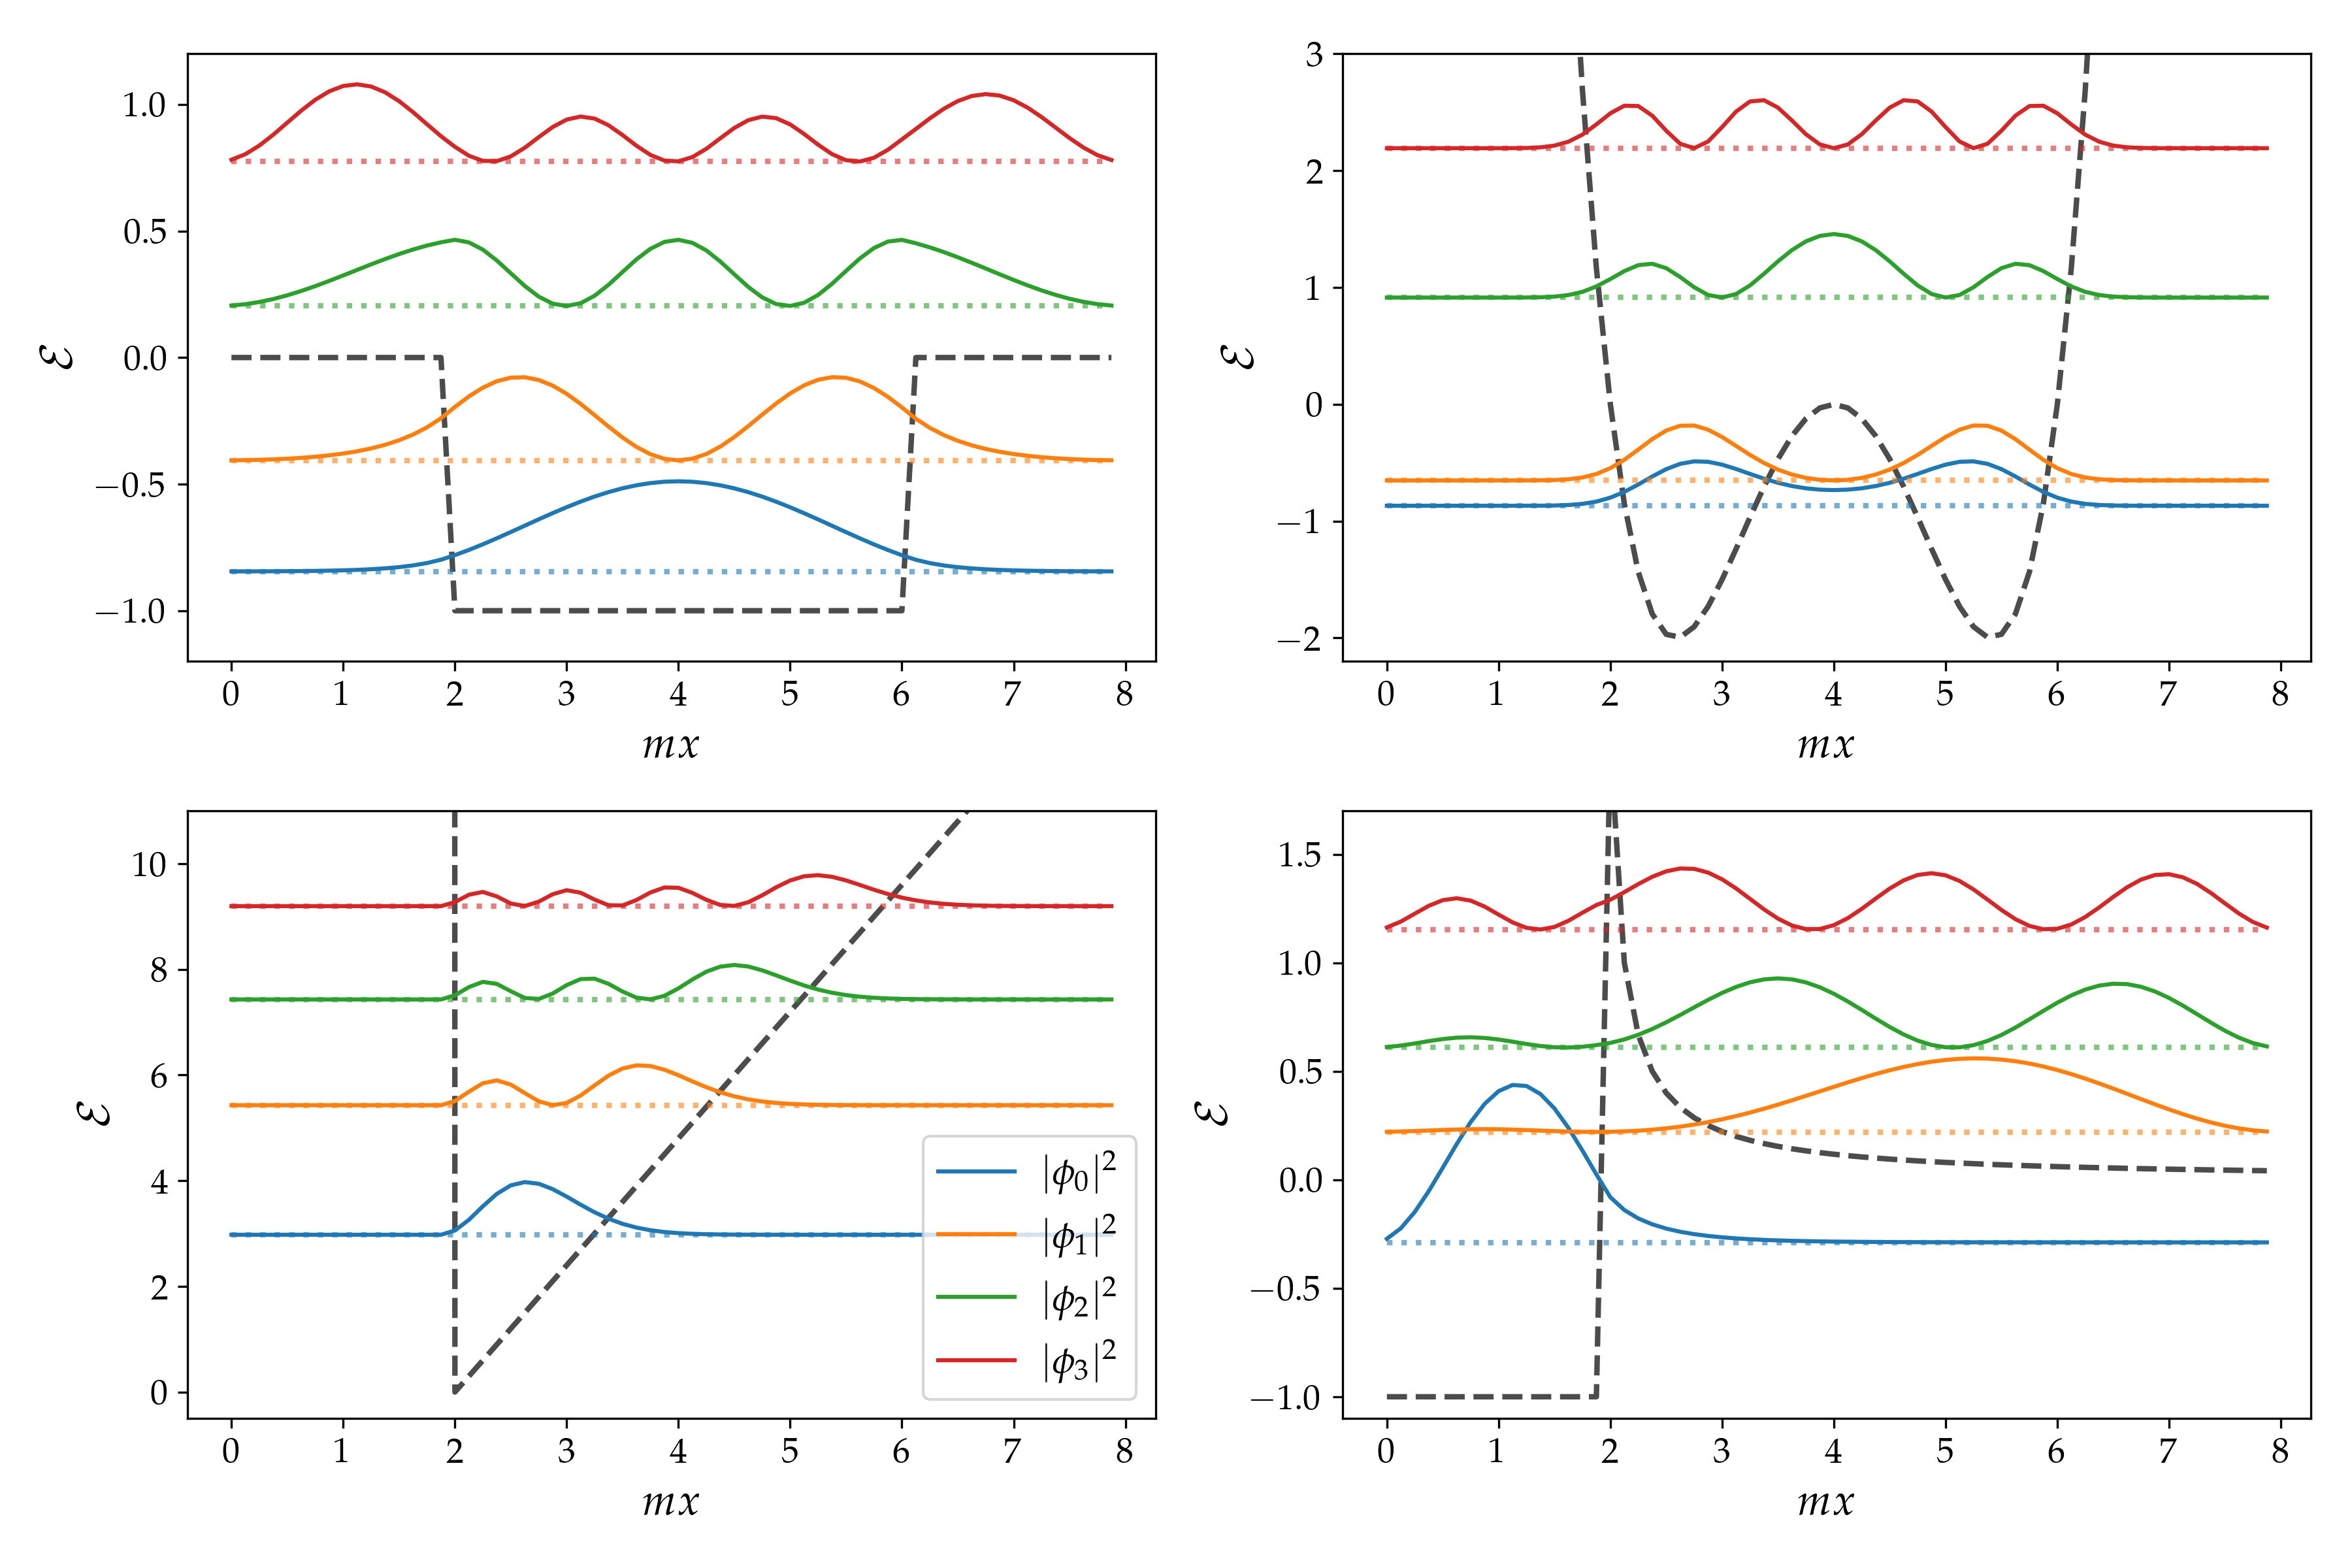
\includegraphics[width=0.85\linewidth]{images/18/comp_Vs_noTitle.png}
        \caption{Autostati per un sistema quantistico 1D con differenti potenziali statici. Sono rappresentati il \textit{Ground State} e i primi 3 stati eccitati. Ulteriori approfondimenti nel Cap. \ref{Cap. Schr t-indep}.}
    \end{figure}
\end{titlepage}

\thispagestyle{empty} 
\null 
\clearpage
\pagestyle{empty} 

\tableofcontents
\clearpage
\pagestyle{plain}

\thispagestyle{empty} 
\null 
\clearpage

% ==================================================
% INCLUSIONE DEI FILE ESTERNI
% ==================================================


% --- PARTE 1: Approssimazione Numerica ---
\cleardoublepage 
\addtocontents{toc}{\bigskip\protect\textbf{\Large Approssimazione Numerica}\par\smallskip}
\addtocontents{toc}{\protect\setcounter{tocdepth}{-2}} 
\part{\Huge Approssimazione Numerica}
\addtocontents{toc}{\protect\setcounter{tocdepth}{2}} 


\section{Esercizio 1.2.1}
\label{sec: basilea}

\subsection{Problem Statement}
Considera la seguente somma

\[
\sum_{n=1}^{\infty} \frac{1}{n^2} = \frac{\pi^2}{6} = \lim_{N \to \infty} S(N) \quad \text{con} \quad S(N) = \sum_{n=1}^{N} \frac{1}{n^2}
\]


\begin{enumerate}
    \item Calcolare la somma in precisione singola usando l'ordinamento normale, ovvero iniziando la sommatoria da $n = 1$, poi $2, \dots$ ($n = 1, 2, \dots N$)
    \item Calcolare la somma in precisione singola usando l'ordinamento inverso, ovvero iniziando la sommatoria da $n = N$, poi $n = N - 1 \dots$ ($n = N, \dots 2, 1$)
    \item Studiare la convergenza di entrambi i metodi in funzione di $N$, graficando $|S(N) - \pi^2/6|$
    \item Ripetere i punti 1, 2 e 3 in precisione doppia
\end{enumerate}

\subsection{Premessa Teorica}
Le variabili rappresentate in precisione singola (32 bit) riservano 23 bit alla mantissa, garantendo circa 7 cifre decimali significative. In precisione doppia (64 bit) si hanno invece circa 15-16 cifre significative. Al limite della rappresentazione numerica corrisponde l'errore di arrotondamento (\textit{round-off error}): le operazioni eseguite dal calcolatore conservano questo errore, che viene propagato e influenza la correttezza del risultato.

Il problema richiede di osservare come agiscono gli errori di arrotondamento in funzione della precisione (32-bit, 64-bit). Si propone di risolvere numericamente il calcolo di $S(N)$; il confronto con il valore analitico permette di calcolare l'errore assoluto come:
\[
    \sigma = |S(N) - \pi^2/6|
\]

\subsection{Metodi Numerici e Algoritmi}
È nostro interesse studiare l'effetto dell'arrotondamento al variare di $N$. Ogni termine $\frac{1}{n^2}$ viene valutato imponendo che numeratore e denominatore siano rappresentati nella precisione scelta.

Nella rappresentazione \textit{floating point}, l'operazione di somma dipende dall'ordine di grandezza degli addendi. Quando si sommano numeri molto diversi, il calcolatore deve allineare le mantisse traslando quella del numero più piccolo; se la differenza di ordini di grandezza supera la capacità della mantissa, il contributo del numero minore viene perso.

\noindent L'ordinamento sequenziale con cui procede la somma può essere quindi non indifferente per gli effetti dell'errore di \textit{round-off}, il limite alla precisione è dettato principalmente dalla \textit{machine precision} ($\epsilon_{single} \approx 1.2 \times 10^{-7}, \epsilon_{double} \approx 2.2 \times 10^{-16}$)
\begin{enumerate}

    \item Per l'ordinamento normale (crescente):
    $$
    \sum_{n=1}^N \frac{1}{n^2} = \frac{1}{1^2} + \frac{1}{2^2} + \dots + \frac{1}{N^2}
    $$
    la somma parziale $S(n)$ cresce rapidamente stabilizzandosi vicino a $1.645$. Per $n$ grande, il termine $\frac{1}{n^2}$ diventa trascurabile rispetto a $S(n)$, portando alla perdita di informazione. Esiste un valore di $n$ oltre il quale la somma non aumenta più.

    \item Nell'ordinamento inverso (decrescente), sommiamo prima i termini piccoli tra loro. Questi accumulano una somma parziale che cresce gradualmente, permettendo di conservare cifre significative che andrebbero perse se sommate singolarmente a un valore già grande, risultando in un metodo più preciso per il calcolo della somma (nel confronto per $N$ grande).
\end{enumerate}

\subsection{Risultati e Discussione}
I risultati ottenuti confermano le previsioni teoriche. inoltre l'andamento dell'errore evidenzia una soglia critica di $N$, dettata dalla precisione di macchina $\epsilon$, oltre la quale il comportamento numerico diverge sensibilmente dal modello analitico.

\subsubsection{$\Tilde{N}_N$}
\noindent Nell'ordinamento normale, la somma parziale $S(N)$ tende rapidamente al valore asintotico $S \approx 1.645$. Un nuovo termine $1/n^2$ viene ignorato dal calcolatore quando il suo rapporto rispetto alla somma parziale scende sotto la soglia della precisione di macchina:$$    \frac{1/n^2}{S(n)} < \epsilon \implies \frac{1}{n^2} \lesssim 1.645 \cdot \epsilon$$

\noindent Approssimando $S(n) \approx 1$, definiamo $\Tilde{N}_N = 1/\sqrt{\epsilon}$ come il valore di saturazione. Oltre questo limite, ogni ulteriore termine è troppo piccolo per modificare la mantissa della somma già accumulata; l'errore $\sigma(N)$ smette quindi di decrescere e rimane costante (plateau visibile nei grafici).
\[
    \epsilon \ge \frac{1}{n^2} \implies n \ge \frac{1}{\sqrt{\epsilon}}= \Tilde{N}_N \\
\]
\[
    \implies S(n) = S(\Tilde{N}_N) \\
\]
\[
    \implies \sigma(n) = \sigma(\Tilde{N}_N)
\]
\smallskip



\begin{figure} [H]
    \centering
    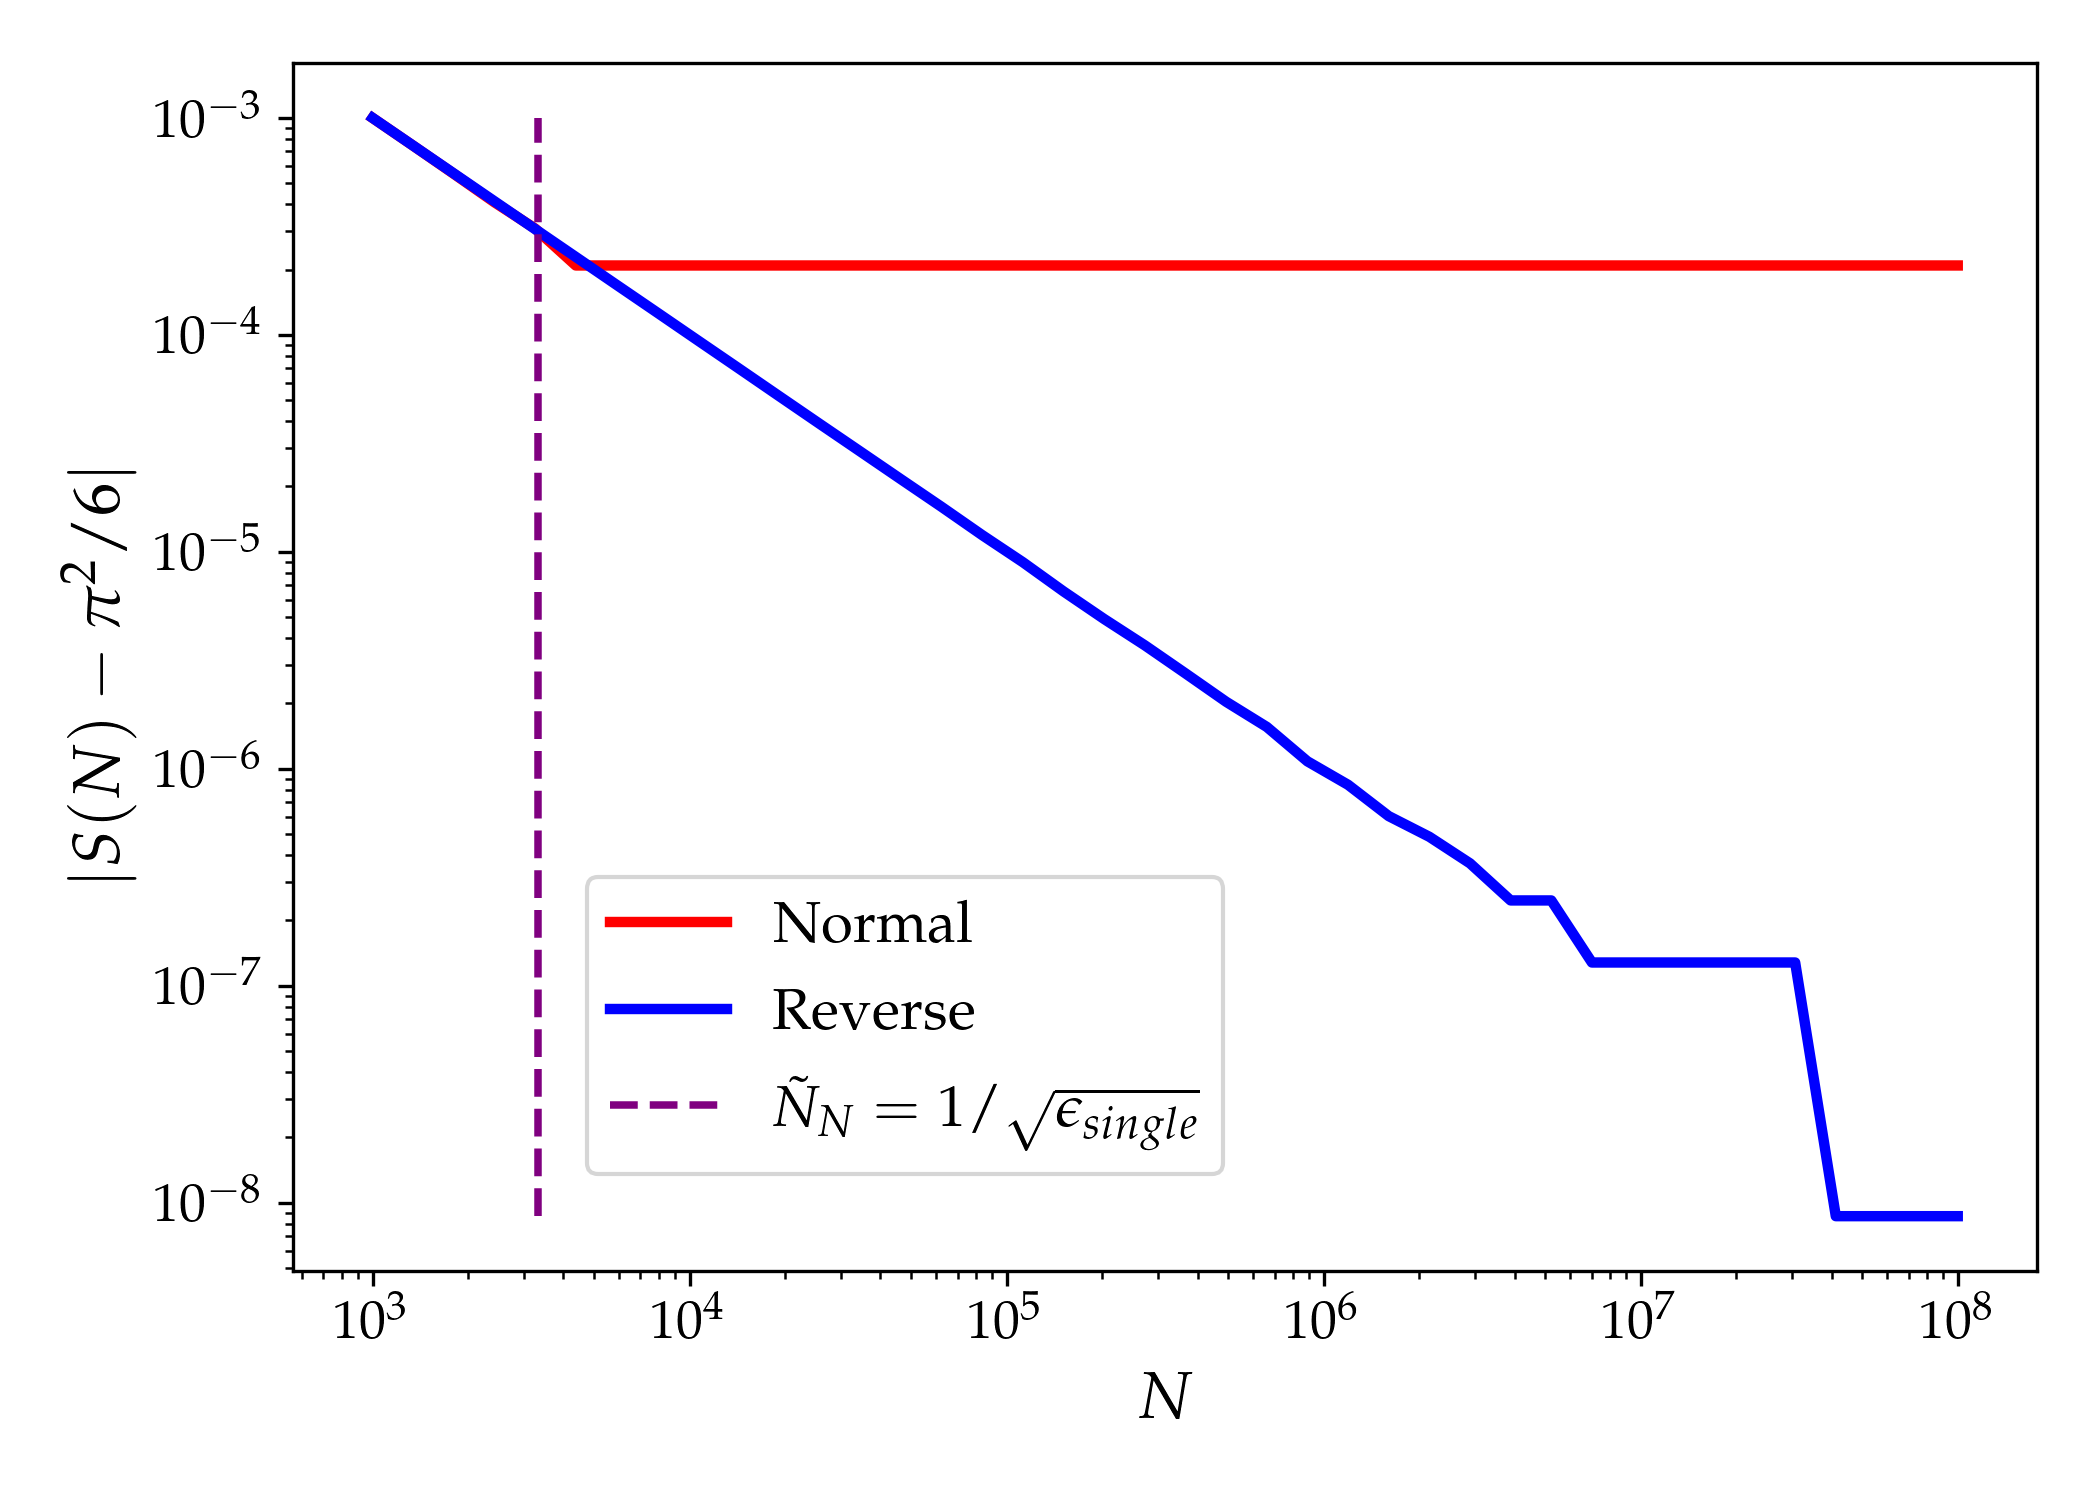
\includegraphics[width=0.7\linewidth]{images/2/SinglePrec.png}
    \caption{Andamento dell'errore assoluto $\sigma(N) = |S(N) - \pi^2 / 6|$ usando lo standard a precisione singola, 32-Bit}
    \label{fig: 1 - single precision}
\end{figure}

\begin{figure} [H]
    \centering
    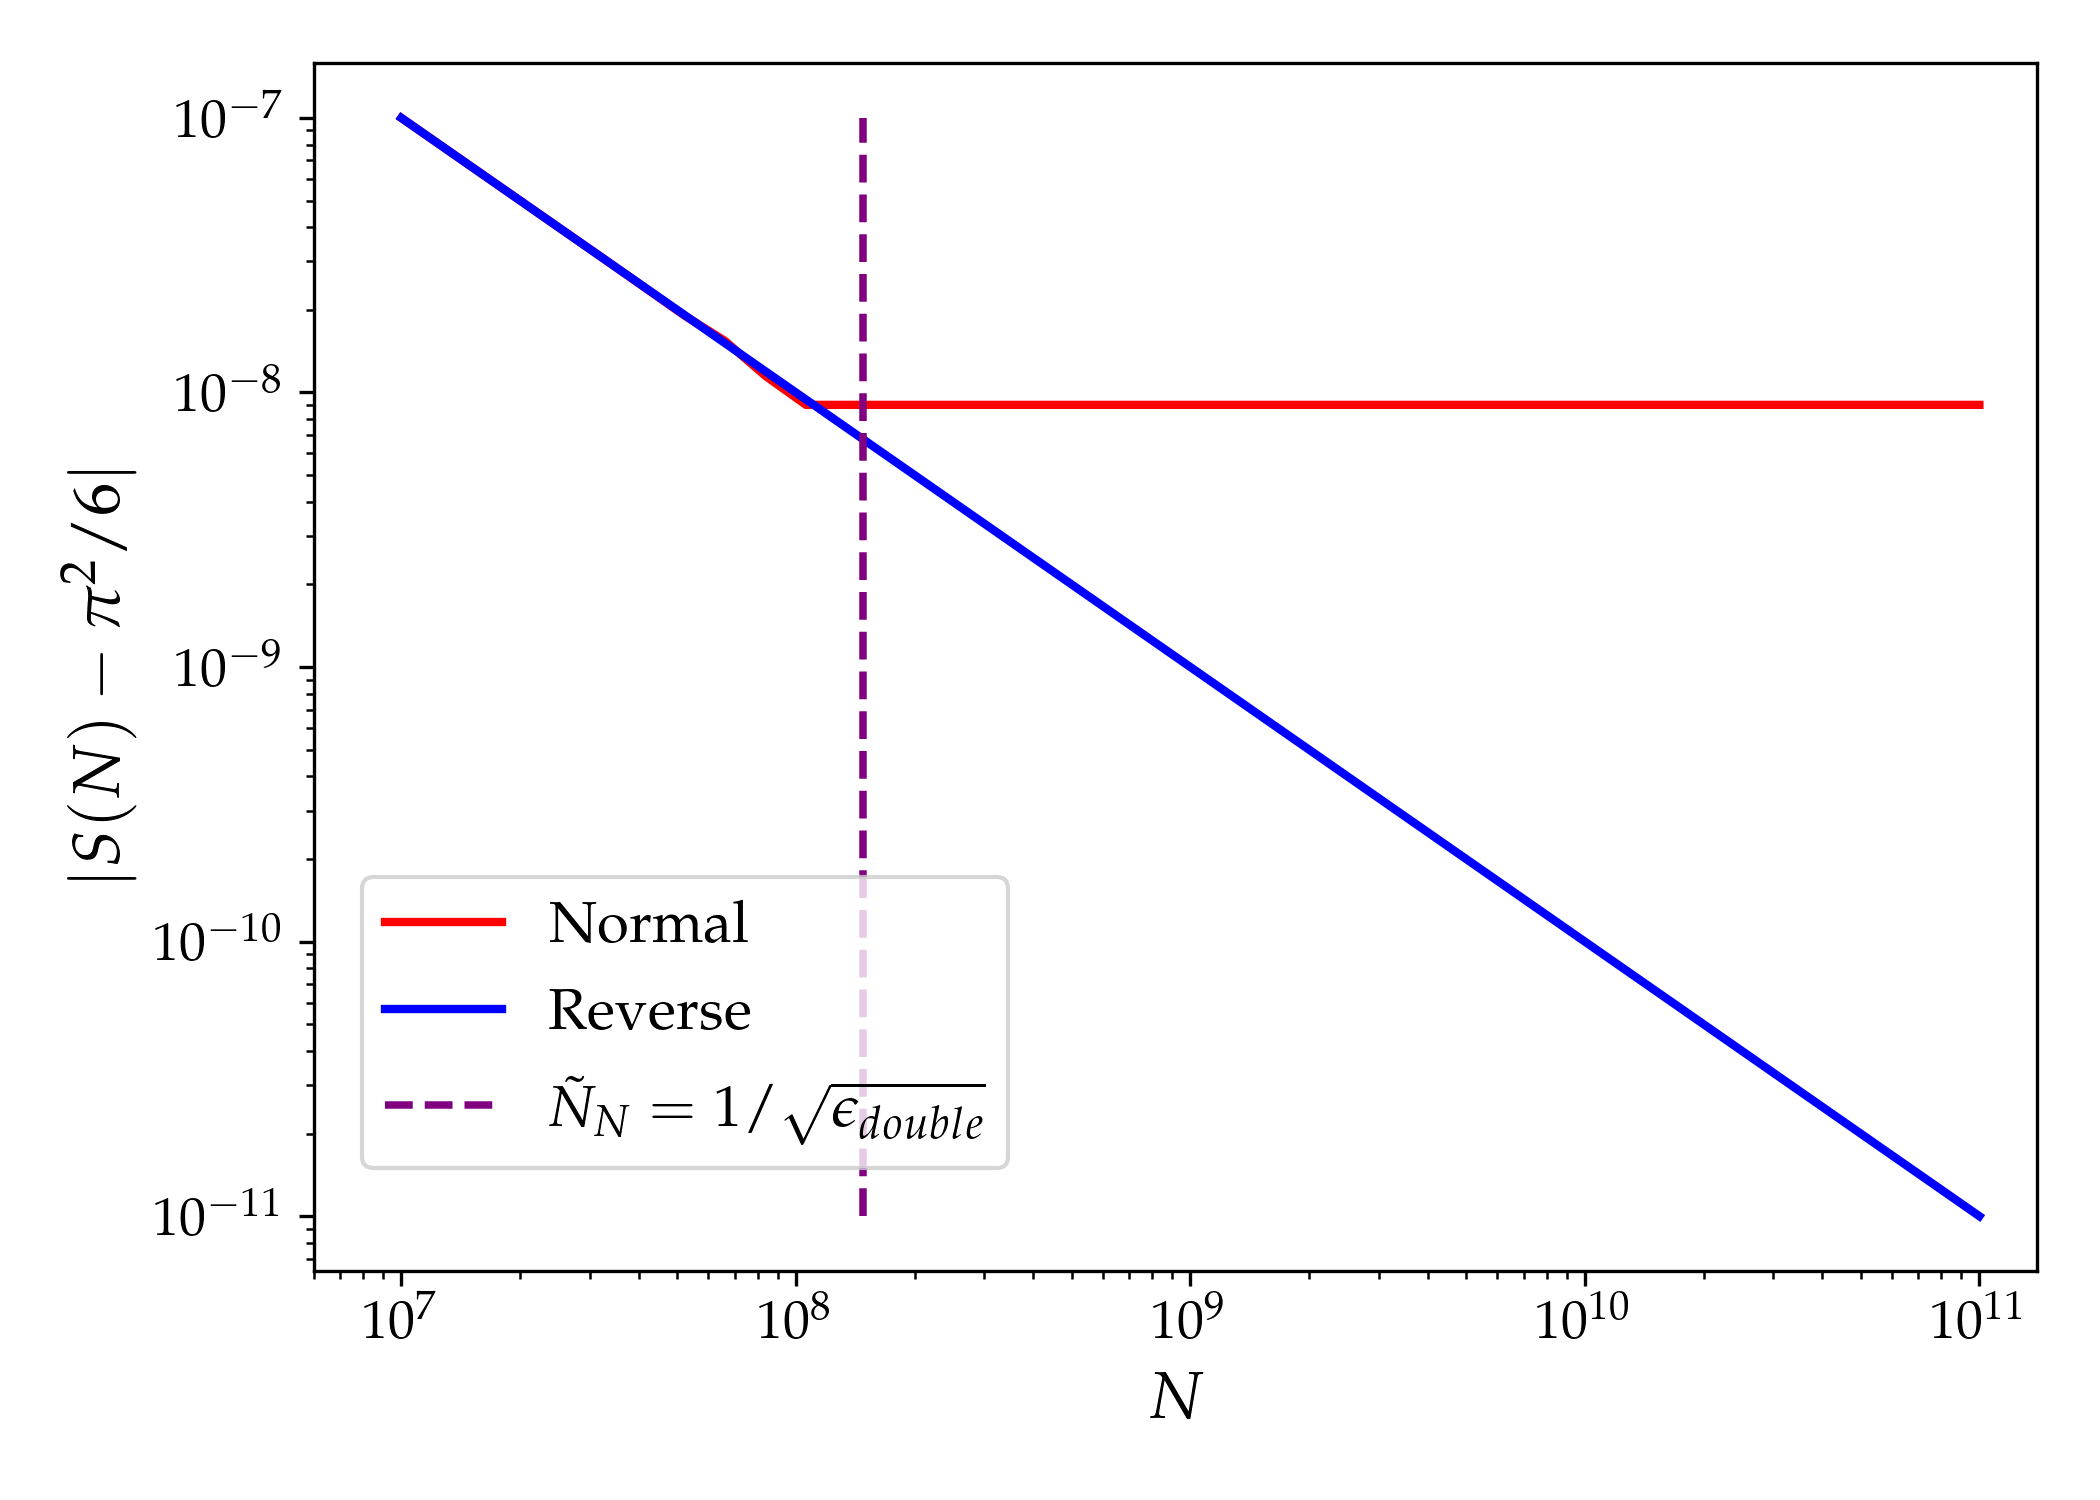
\includegraphics[width=0.7\linewidth]{images/2/DoublePrec.png}
    \caption{Andamento dell'errore assoluto $\sigma(N) = |S(N) - \pi^2 / 6|$ usando lo standard a precisione doppia, 64-Bit}
    \label{fig: 2 - double precision}
\end{figure}


\newpage
% \thispagestyle{empty} 
\null 
\clearpage

% --- PARTE 2: Matrici e Sistemi Lineari ---
\cleardoublepage 
\addtocontents{toc}{\bigskip\noindent\protect\textbf{\Large Matrici e Sistemi Lineari}\par\smallskip}   
\addtocontents{toc}{\protect\setcounter{tocdepth}{-2}} 
\part{\Huge Matrici e Sistemi Lineari} \label{Cap: Matrici e Sistemi Lineari}
\addtocontents{toc}{\protect\setcounter{tocdepth}{2}} 

\section{Esercizio 2.1.1}

\subsection{Problem Statement}
\begin{enumerate}
    \item \textbf{Scrivere una funzione} che accetti una matrice triangolare superiore e implementi la backward substitution. Testarla sul sistema lineare $U\mathbf{x} = \mathbf{b}$ con
    \[
        U = \begin{pmatrix} 2 & 1 & 1 \\ 0 & 1 & -2 \\ 0 & 0 & 1 \end{pmatrix}, \quad \mathbf{b} = \begin{pmatrix} 1 \\ -1 \\ 4 \end{pmatrix}
    \]
    e verificare che la soluzione sia corretta.

    \item \textbf{Scrivere una funzione separata} che esegua la Gauss elimination e combinarla con la Backward substitution per risolvere il sistema
    \[
        \begin{pmatrix} 2 & 1 & 1 \\ 1 & 1 & -2 \\ 1 & 2 & 1 \end{pmatrix} \begin{pmatrix} x_0 \\ x_1 \\ x_2 \end{pmatrix} = \begin{pmatrix} 8 \\ -2 \\ 2 \end{pmatrix}
    \]
    Verificare la soluzione. 

    \item \textbf{Utilizzando i programmi precedenti}, aggiungere una funzione che stampi anche l'inversa esplicita di una matrice. Testarla sulla matrice sopra indicata e verificare il risultato.

    \item \textbf{Adattare i programmi precedenti} per includere il partial pivoting e risolvere i seguenti sistemi. Verificare che senza partial pivoting il programma fallisca, poiché in qualche passaggio intermedio appare $A_{jj} = 0$ per la matrice
    \[
        \begin{pmatrix} 2 & 1 & 1 \\ 2 & 1 & -4 \\ 1 & 2 & 1 \end{pmatrix} \begin{pmatrix} x_0 \\ x_1 \\ x_2 \end{pmatrix} = \begin{pmatrix} 8 \\ -2 \\ 2 \end{pmatrix}
    \]

    \item \textbf{Studiare la soluzione} del problema
    \[
        \begin{pmatrix} 10^{-20} & -1 \\ 1 & 1 \end{pmatrix} \begin{pmatrix} x_0 \\ x_1 \end{pmatrix} = \begin{pmatrix} 1 \\ 2 \end{pmatrix}
    \]
    con e senza pivoting. In questo caso il sistema non è mal condizionato (ovvero non genera infiniti), ma produce un risultato errato. Spiegare l'origine dell'errore e perché il pivoting lo risolve.
\end{enumerate}

\subsection{Premessa Teorica}
Lo scopo dell'esercizio è quello di mettere in luce il più semplice dei metodi numerici per la risoluzione di sistemi lineari di equazioni, sfruttando il formalismo matriciale, risolvendo quindi:
$$
Ax=b
$$
$A$ matrice (quadrata) dei coefficienti, $x$ vettore delle soluzioni (da determinare), $b$ vettore dei termini noti
\subsection{Metodi Numerici e Algoritmi}
\subsubsection{Backward/Forward substitution} \label{sec: Back-Forw Subst}
L'algoritmo fondamentale che usiamo è quello di \textit{Backward/Forward substitution}, cioè che risolve sistemi lineari costruiti da una matrice dei coefficienti che è triangolare superiore/inferiore. Il termine dell'ultima/prima riga è determinabile direttamente, risolvendo $x_i = \frac{b_i}{L_{ii}}$, poi si procede risolvendo per ogni riga in maniera sequenziale e determinando l'intero vettore $x$.\\Per la \textit{Backward} la formula generale è:
$$
x_i = \left( b_i - \sum_{j=i+1}^{n-1} U_{ij}x_j \right) \frac{1}{U_{ii}} \quad i = n-1, \dots , 0
$$
per la \textit{Forward}:
$$
x_i = \left( b_i - \sum_{j=0}^{i-1} L_{ij}x_j \right) \frac{1}{L_{ii}} \quad i = 0, \dots, n-1
$$

\subsubsection{Gaussian Elimination}
Si può generalizzare la soluzione di un sistema lineare per una matrice $A$ quadrata generica. Per fare ciò usiamo un algoritmo che permetta di riportare $A$ nella forma di $U$ (triangolare superiore), in maniera da poter risolvere usando la \textit{Backward substitution}. È possibile sviluppare l'algoritmo partendo da semplici operazioni sulle matrici, nel corso delle quali si sceglie una riga di riferimento (pivot row) e la si usa per annullare tutti gli elementi delle righe al di sotto di questa. Ci si sposta quindi nella riga successiva, fino a che non si rende $A$ una triangolare superiore. Si possono quindi combinare \textit{Gaussian elimination} (GE) e \textit{Backward substitution} (BS) in una unica funzione.

\subsubsection{Partial Pivoting}
In caso di matrici mal condizionate, può accadere che la scelta del \textit{pivot} non sia irrilevante: in questi casi, l'operazione di \textit{Partial pivoting} (PP) permette di stabilizzare il processo, scambiando la riga pivot \textit{p}, nella colonna \textit{j}, con la riga \textit{i} con l'elemento $A_{ij}$ massimo rispetto a quelli nella colonna.

\subsubsection{Inversa di una Matrice} \label{sec: inverse of a matrix}
Combinando gli algoritmi sopra definiti è possibile anche determinarne uno per trovare l'inverso di una matrice generica $A$. Data la generica $A\in \mathbb{C}^{n\times n}$ e $\mathbb{I}_n$, matrice identità:
$$
A^{-1} = (x_0,\ x_1,\ \dots\ , x_{n-1})
$$

\noindent cioè la colonna i-esima della matrice $A^{-1}$ sarà data dalla soluzione al sistema 
$$
A\ x_i = \mathbb{I}_i  
$$
dove $\mathbb{I}_i$ è la colonna i-esima della matrice identità.

\newpage

\subsection{Risultati e Discussione}
Di seguito i risultati e le soluzioni ai problemi presentati nella consegna:
\begin{multicols}{2} % Inizio delle due colonne
\begin{enumerate}[series=miolista]

   \item Risoluzione del sistema $Ux = b$ tramite BS:
    \begin{elegantcode}
U =
 [[ 2.  1.  1.]
 [ 0.  1. -2.]
 [ 0.  0.  1.]]
b = [ 1. -1.  4.]

Solution found:
x = [-5.  7.  4.]
    \end{elegantcode}

\item Risoluzione del sistema generico tramite GE e BS; usiamo una versione di GE "ingenua":

\begin{elegantcode} 
A =
 [[ 2.  1.  1.]
 [ 1.  1. -2.]
 [ 1.  2.  1.]]
b = [ 8. -2.  2.] 

x = [ 4. -2.  2.]
    \end{elegantcode}

    \item L'inversa può essere determinata come definito nell'algoritmo in \ref{sec: inverse of a matrix}:
    \begin{elegantcode} 
A =
 [[ 2.  1.  1.]
 [ 1.  1. -2.]
 [ 1.  2.  1.]] 

Solution found:
A^-1 =
 [[ 0.625  0.125 -0.375]
 [-0.375  0.125  0.625]
 [ 0.125 -0.375  0.125]]
    \end{elegantcode}

    \item La prova del fallimento dell'algoritmo "ingenuo" determina la necessaria modifica a GE per introdurre PP e generalizzare il suo utilizzo:

    \begin{elegantcode}[title=Uso di \textit{BackGauss\_dumb()} e problemi relativi agli infiniti]
An error occured!!: Algorithm fails!
b != U * x 
RuntimeWarning: divide by zero encountered in scalar divide
  c = A[i,j] / A[j,j]
RuntimeWarning: invalid value encountered in multiply
  A[i,:] -= c * A[j,:]
RuntimeWarning: invalid value encountered in scalar divide
  x_i = (b[i] - np.dot(U[i, i+1:], np_xi[i+1:])) / U[i, i]
    \end{elegantcode}

    \begin{elegantcode}[title=Uso di \textit{BackGauss()} per trovare la soluzione del problema (implementazione di PP)]
A =
 [[ 2.  1.  1.]
 [ 2.  1. -4.]
 [ 1.  2.  1.]]
b = [ 8. -2.  2.] 

Solution:
x = [ 4. -2.  2.]
    \end{elegantcode}
\end{enumerate}
\end{multicols}

\begin{enumerate}[resume=miolista]
    \item Il pivoting garantisce stabilità anche con matrici non mal condizionate, evitando errori di assorbimento in virgola mobile. Analiticamente:
    \[
    \begin{pmatrix} 10^{-20} & -1 \\ 1 & 1 \end{pmatrix}
    \begin{pmatrix} x_0 \\ x_1 \end{pmatrix} =
    \begin{pmatrix} 1 \\ 2 \end{pmatrix} \implies
    \begin{cases} x_0 = 3 \\ x_1 = -1 \end{cases}
    \]

    Nell'esecuzione del programma senza pivoting il problema si incontra nel momento in cui, tenendo come pivot la prima riga, svolgiamo:
    $$c =\frac{A_{10}}{A_{00}}=10^{20} \implies
    \begin{cases}
        A_{10} = 0 \\
        A_{11} = 1+10^{20}\\
        b_1 = 2-10^{20}
    \end{cases}    
    $$    
    Dall'analisi dei risultati emerge chiaramente la criticità intrinseca nelle operazioni effettuate. Nello specifico, il calcolo di espressioni quali $1+10^{20}$ o $2-10^{20}$ evidenzia i limiti strutturali della rappresentazione numerica finita.
    
    L'elaboratore opera in precisione doppia, uno standard che garantisce una risoluzione di circa 15-16 cifre significative. Quando si confrontano operandi che differiscono per 20 ordini di grandezza, il valore minore scende al di sotto della precisione di macchina ($\epsilon_m$). 
    
    Di conseguenza, durante l'allineamento delle mantisse, il numero più piccolo viene "assorbito" da quello maggiore, rendendo l'operatore insensibile alla variazione. Si verifica pertanto il fenomeno dell'errore di arrotondamento per cui:
    
    $$
    \begin{cases}
        A_{11} = 1+10^{20} \approx 10^{20}\\
        b_1 = 2-10^{20} \approx -10^{20}
    \end{cases}    
    $$    
    
    $$
        \begin{pmatrix}
            10^{-20} & -1 \\
            0 & 10^{20}
        \end{pmatrix}
        \begin{pmatrix}
            x_0 \\x_1
        \end{pmatrix} =
        \begin{pmatrix}
            1 \\ -10^{20}
        \end{pmatrix}
    $$
    $$
    \implies \begin{cases}
        x_1 = \frac{-10^{20}}{10^{20}} = -1 \\
        x_0 = \frac{1 - x_1}{10^{-20}} = 0 
    \end{cases}
    $$
    cioè un risultato inesatto! Il metodo senza PP ci conduce a sbagliare nettamente la risposta al problema.
        
    \noindent L'output generato dall'esecuzione degli script conferma l'analisi precedente:\\
    
    \begin{elegantcode}
# Senza Pivoting (Errore)
x_dumb = [ 0. -1.]
# Con PP (Corretto)
x_true = [ 3. -1.]
    \end{elegantcode}
    
    \noindent L'esperimento dimostra che una matrice non mal condizionata (il cui determinante è significativamente diverso da zero) può comunque portare al fallimento dell'algoritmo di Gauss se non si adotta il pivoting parziale.
    
\end{enumerate}
\newpage





\section{Esercizio 2.2.1}
\label{sec: poisson res}
\subsection{Problem Statement}
Scrivere un programma che accetti una matrice $A$, verifichi che sia simmetrica (se reale) e restituisca quindi il fattore di Cholesky $L$.

\begin{enumerate}
    \item Testare il programma sulla matrice
    \[
    \begin{pmatrix}
    4 & 12 & -16 \\
    12 & 37 & -43 \\
    -16 & -43 & 98
    \end{pmatrix}
    \]
    e verificare la correttezza del risultato.
    
    \item Scrivere un risolutore che combini la fattorizzazione di Cholesky con le \textit{forward} e \textit{backward substitution}.
    
    \item Calcolare la matrice laplaciana $K$ e il vettore $b$ utilizzando
    \begin{itemize}
        \item $4\pi\varepsilon_0 = 1.0$
        \item $L = 1.0$
        \item $N = 50$
        \item densità di carica distribuita gaussianamente $\rho(x) = e^{-R(x-0.5)^2}$
    \end{itemize}
    
    Risolvere il sistema lineare per i casi $R = 100$ e $R = 10$ utilizzando il risolutore basato sulla decomposizione di Cholesky.
\end{enumerate}


\subsection{Premessa Teorica} \label{Cap: Cholesky}
Una matrice non singolare $A$ può essere espressa come prodotto di due matrici triangolari, inferiore e superiore, cioè:
\[
A = LU
\]
dove questa cosiddetta \textit{decomposizione LU} non è unica: è imponendo alcune condizioni che possiamo determinare univocamente le due, quindi possiamo risolvere il sistema generico 
\[
Ax = b
\]
eseguendo una combinazione di BS e FS. \textit{Il teorema di decomposizione di Cholesky} afferma inoltre che per una qualsiasi matrice hermitiana definita positiva esiste ed è unica la matrice $L$ (Fattore di Cholesky) t.c.:
\[
A = LL^\dagger
\]

\subsection{Metodi Numerici e Algoritmi}
Analizzando la definizione di $A=LL^\dagger$, esprimendo esplicitamente il prodotto delle due matrici a destra, si può evidenziare come sia possibile determinare $L$ con una funzione ricorsiva partendo solo da $A$, iterando sulle sue righe e colonne. Ciò permette di risolvere il sistema lineare, in particolare:
\[
Ax = LL^\dagger x = Ly = b\ , \quad L^\dagger x = y
\]
\[
\begin{cases}
    Ly = b \quad (\text{FS, ricavo $y$})\\
    L^\dagger x = y \quad (\text{BS, ricavo $x$})
\end{cases}
\]
al termine della seconda iterazione ho quindi determinato univocamente le soluzioni del sistema lineare definito inizialmente su $A$, matrice dei coefficienti.
\\
Se dal punto di vista del costo computazionale questo approccio presenta un leggero guadagno rispetto a quello della LU (entrambi proporzionali a $n^3$) la vera grande differnza sta nella stabilità dell'algoritmo della \textit{decomposizione di Cholesky}: di fronte ad una matrice $A$ mal condizionata, quindi con un $\kappa(A)$ grande, $L$ è in generale proporzionale al \textit{condition number}, ma il prodotto $LL^\dagger$ presenta molte semplificazioni che determinano:
\[
\Tilde{L}\Tilde{L}^\dagger = A + \delta A
\]
dove $\Tilde{L}$ è il \textit{Cholesky factor} di $A$ più una sua piccola variazione. La variazione su $A$ può modificare anche significativamente $L$, ma il prodotto con la sua aggiunta differisce dal risultato imperturbato di una piccola quantità, proprio grazie alle semplificazioni nel calcolo del prodotto che bilanciano l'operazione.

\subsection{Risultati e Discussione}
\begin{enumerate}
   \item Test di funzionamento della funzione per $L$
    \begin{elegantcode} 
A:
 [[  4.  12. -16.]
 [ 12.  37. -43.]
 [-16. -43.  98.]]

Cholesky factor (L):
 [[ 2.  0.  0.]
 [ 6.  1.  0.]
 [-8.  5.  3.]]
    \end{elegantcode}
    Il test di correttezza del risultato avviene confrontando $LL^\dagger$ con $A$ e aspettandosi una differenza confrontabile con zero tra le due matrici.

    \item Il problema richiede la risoluzione dell'\textit{Equazione di Poisson} (\ref{eq: Poisson}) per via numerica: questo è un caso ottimo per sfruttare le potenzialità dell'algoritmo che abbiamo mostrato, in particolare perché la soluzione di
    \begin{equation} \label{eq: Poisson}
        \nabla^2 \phi\text{(r)} = -\frac{\rho\text{(r)}}{4\pi\varepsilon_0}
    \end{equation}
    può essere ricavata discretizzando il dominio e approssimando la derivata seconda con il metodo delle differenze finite
    \footnote{Secondo le differenze finite:
    $\frac{d^2\phi}{dx^2} \approx \frac{\phi_{i-1} - 2\phi_i + \phi_{i+1}}{a^2}$
    }
    . Inoltre imponiamo le \textit{NU} ($4\pi \varepsilon_0 = 1$) per praticità; risulta quindi
    $$
    -\phi_{i-1} + 2\phi_i - \phi_{i+1} = a^2\rho_i
    $$
    Imponendo le condizioni al contorno $\phi(0)=\phi(L)=0$ e assorbendo $a^2$ nella definizione di $\rho$ ($\rho \leftarrow{} a^2 \rho$) otteniamo un sistema di equazioni lineari in forma matriciale:
    
    \begin{equation} \label{eq: eq lin poisson}    
    K\phi = b
    \end{equation}

    $$
    K = \begin{pmatrix}
        2 & -1 & 0 & \dots & 0 \\
        -1 & 2 & -1 & \dots & 0 \\
        0 & -1 & 2 & \dots & 0 \\
        \vdots &&& \dots & -1 \\
        0 & \dots & \dots & -1 & 2 \\
    \end{pmatrix},\ \ \ b = \begin{pmatrix}
        \rho_1 \\ \rho_2 \\ \vdots \\ \rho_N
    \end{pmatrix}    
    $$
    
    Dove $K$ è la rappresentazione matriciale dell'operatore laplaciano e $b$ è il vettore discretizzato della densità di carica. Saremo agili nel risolvere il sistema lineare (\ref{eq: eq lin poisson}) con i metodi sviluppati finora; in particolare useremo la decomposizione di Cholesky.

    Definendo una distribuzione di carica gaussiana intorno all'origine, come da consegna:
    \[
    \rho(x) = e^{-R(x-0.5)^2} \text{, \quad}\  x \in [0, L]\ \xrightarrow{\text{norm.}}x/L \in [0, 1] 
    \]
    È possibile osservare la soluzione dell'equazione di Poisson nella figura qui sotto; al variare del parametro $R$ il profilo di $\phi$, potenziale generato dalla carica $\rho$.
    \begin{center}
        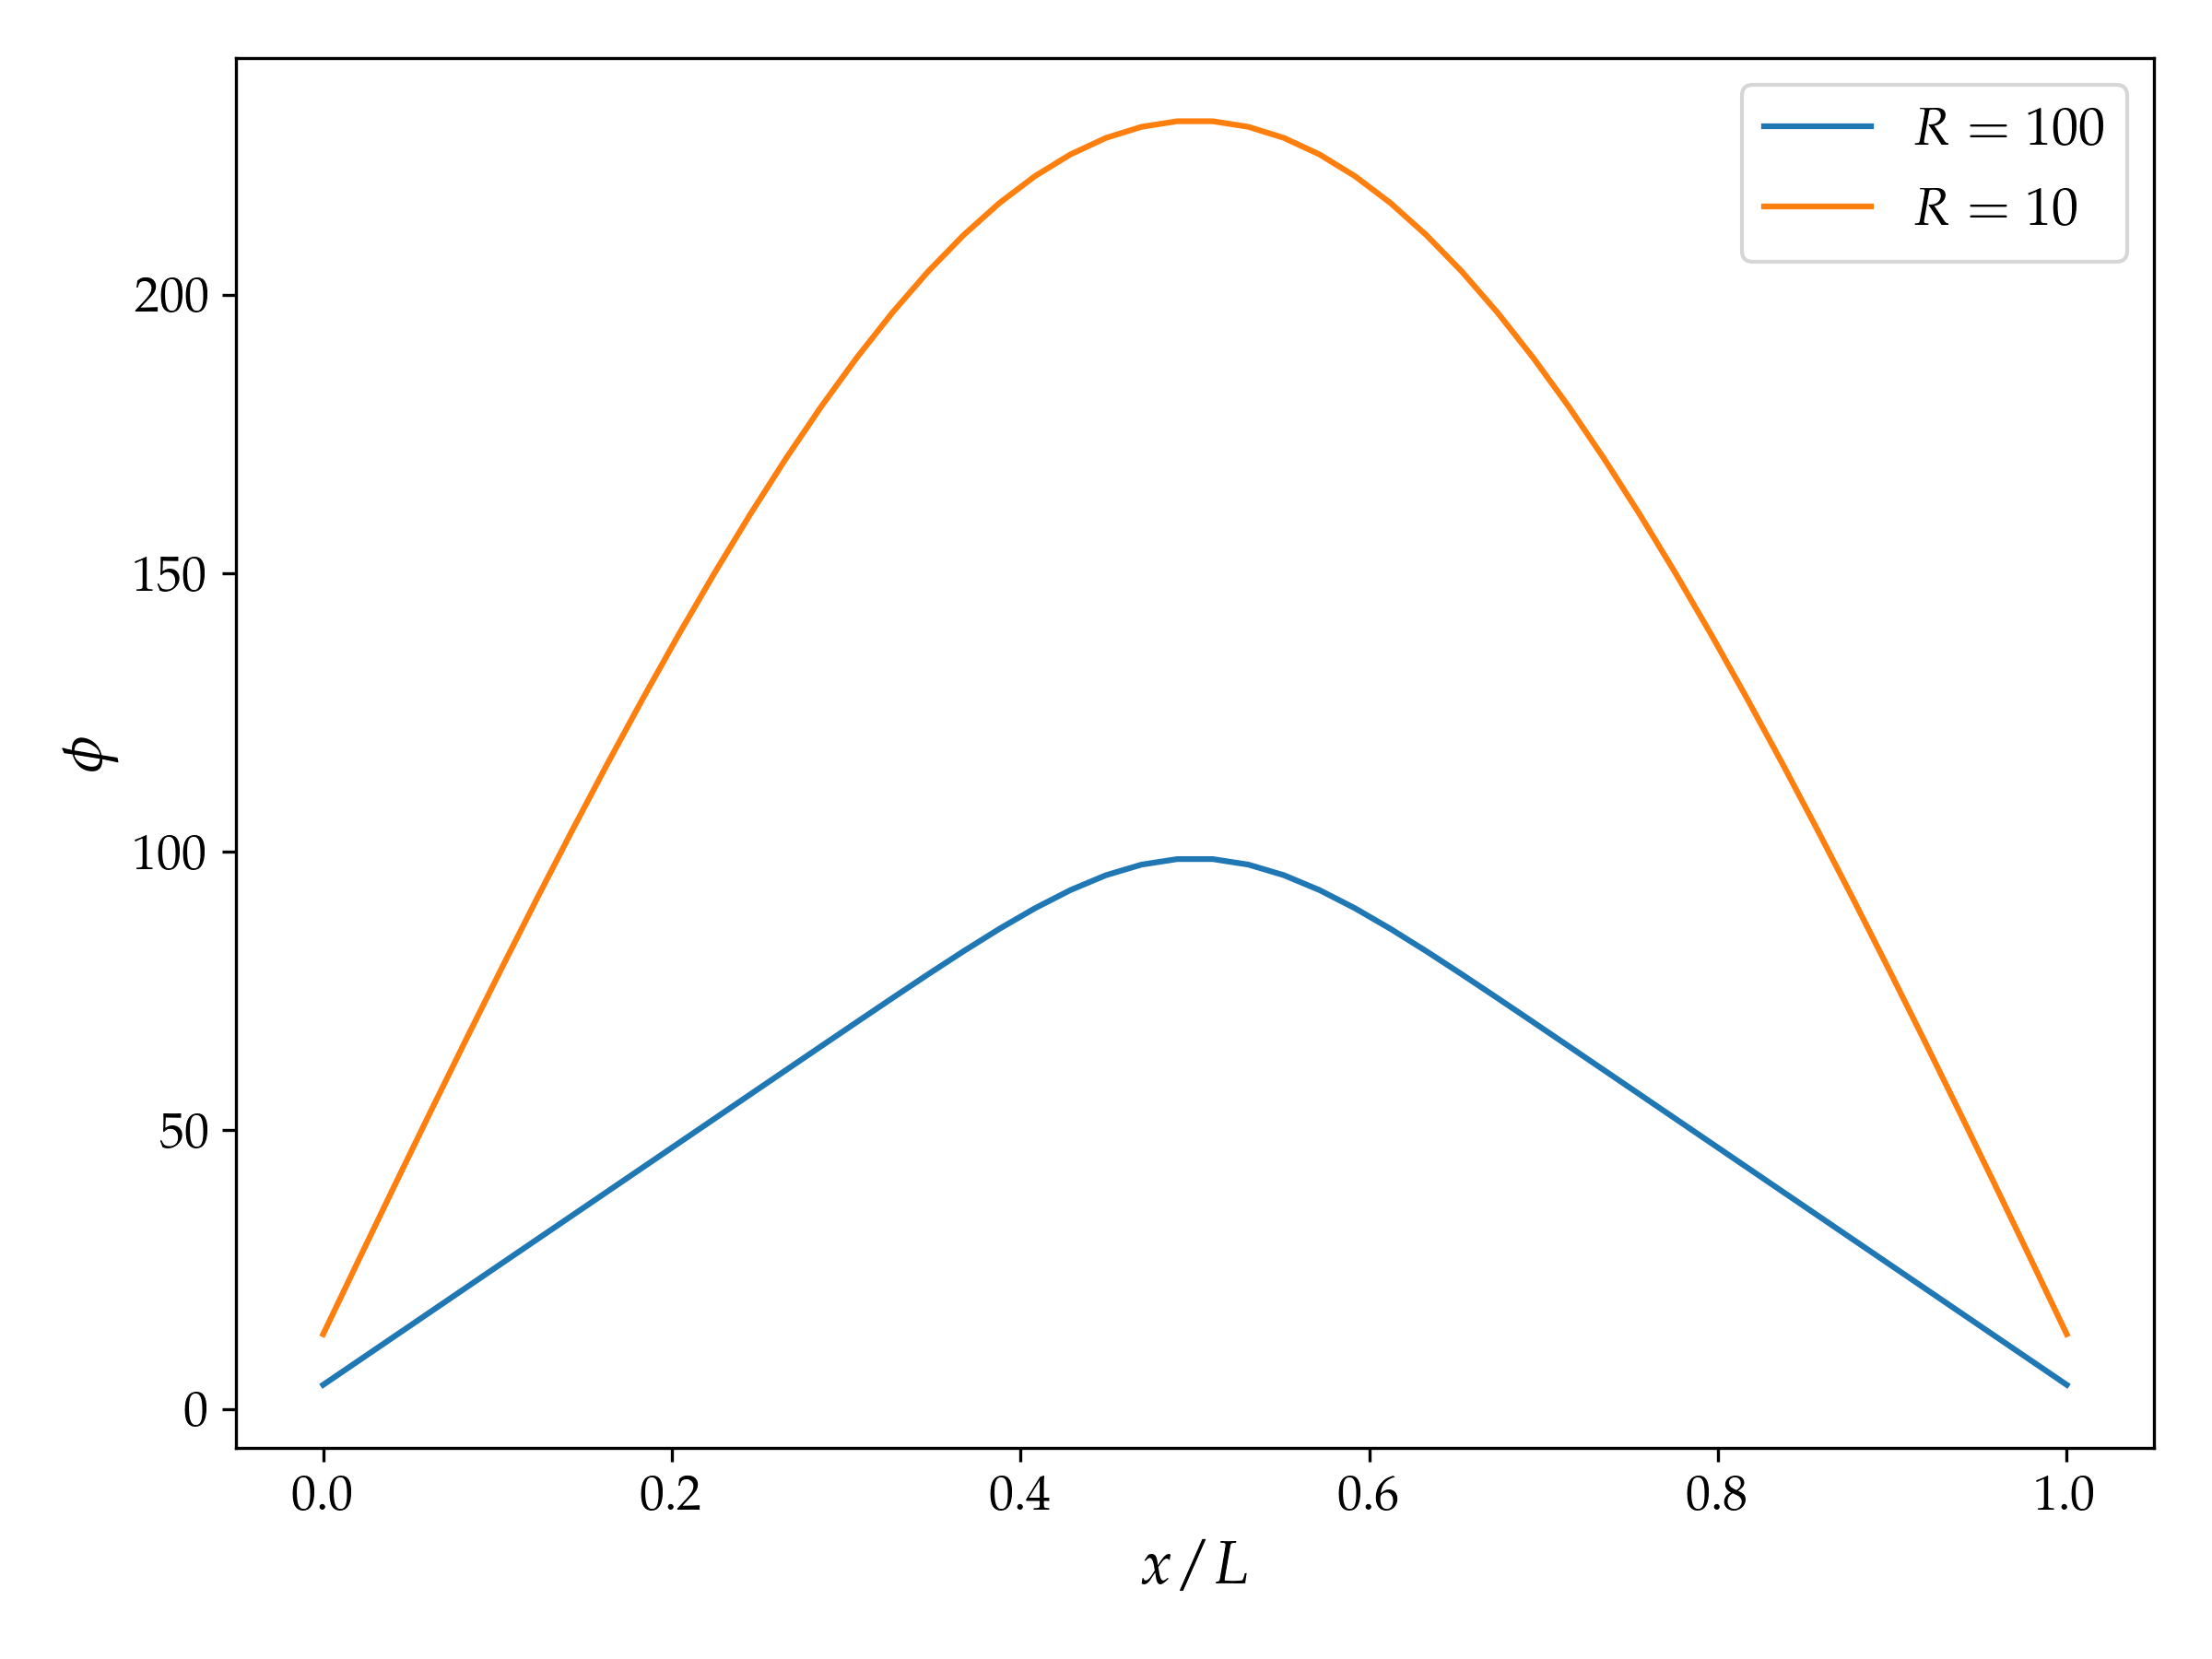
\includegraphics[width=0.7\linewidth]{images/4/poiss_sol.png}
        \captionof{figure}{Soluzione dell'equazione di Poisson $\phi$ per $R=100$ e $R=10$} 
        \label{fig: poiss_label}
    \end{center}
\end{enumerate}

\newpage




\newpage
% \thispagestyle{empty} 
\null 
\clearpage

% --- PARTE 3: Ricerca degli Autovalori ---
\cleardoublepage 
\addtocontents{toc}{\bigskip\noindent\protect\textbf{\Large Ricerca degli Autovalori}\par\smallskip}
\addtocontents{toc}{\protect\setcounter{tocdepth}{-2}} 
\part{\Huge Ricerca degli Autovalori}
\addtocontents{toc}{\protect\setcounter{tocdepth}{2}} 
\label{cap: Autovalori}


\section{Esercizio 3.1.1}
\subsection{Problem Statement}

Considera la matrice
\[
A = \begin{pmatrix}
4 & -i & 2 \\
i & 2 & 2 + 7i \\
2 & 2 - 7i & -2
\end{pmatrix}
\]

\begin{enumerate}
    \item Calcola l'autovalore massimo e il corrispondente autovettore utilizzando il \textit{Power Method}. Introduci un criterio di arresto basato su una data tolleranza sull'autovalore, ad esempio $10^{-6}$, o basato su un numero massimo di iterazioni. Verifica la correttezza dell'algoritmo.
    
    \item Calcola l'autovalore minimo con il \textit{Inverse Power Method} utilizzando il risolutore QR sviluppato negli esercizi precedenti.
    
    \item Studia numericamente la convergenza degli algoritmi. Definisci $\lambda_1^n$ come l'autovalore massimo ottenuto dal \textit{Power Method} dopo $n$ iterazioni e $\lambda_3^n$ come l'autovalore minimo ottenuto dall'\textit{Inverse Power Method}. Successivamente, rappresenta graficamente $|\lambda_1^n / \lambda_1 - 1|$ e $|\lambda_3^n / \lambda_3 - 1|$ in funzione delle iterazioni.
\end{enumerate}

\subsection{Premessa Teorica}
Il \textit{Power Method} (\textit{PM}) è uno degli algoritmi più semplici per estrarre gli autovalori di una generica matrice $A \in \mathbb{C}^{N \times N}$ diagonalizzabile e con un autovalore dominante in modulo, in particolare, il metodo restituisce una stima dell'autovalore di modulo maggiore. È possibile definire un \textit{Inverse Power Method} (\textit{IPM}) che determini l'autovalore minimo della matrice. Questi vengono definiti algoritmi iterativi, cioè che determinano il risultato con uno specifico grado di precisione, ma non convergono in un numero finito di passaggi al valore vero. Nel corso della discussione dei metodi presenentiamo il caso di matrice reale per semplicità: il passaggio ad una complessa richiede di sostituire $A^T \longrightarrow A^\dagger$.

\subsection{Metodi Numerici e Algoritmi}
\subsubsection{Power Method}
Data $A^{N\times N}$ e scegliendo un generico vettore di partenza $\boldsymbol{x_0}$, possiamo definire:
\[
\boldsymbol{y}(n) = A^n \boldsymbol x_0 = \dots = \lambda_1^n \left[ c_1 \boldsymbol{v}_1 + \sum_{i=2}^{N} c_i \left( \frac{\lambda_i}{\lambda_1} \right)^n \boldsymbol{v}_i \right], \quad \quad \left| \frac{\lambda_i}{\lambda_1} \right| < 1
\]
quindi, grazie all'ultima riscrittura, prendendo il limite per $n \xrightarrow{} \infty$, cioè per un grande numero di iterazioni dell'algoritmo:
\begin{equation} \label{eq: Direct Method autovett}
\lim_{n \xrightarrow{}\infty} \boldsymbol{y}(n) = c_1 \lambda_1^n \boldsymbol{v}_1
\end{equation}
L'ultimo risultato ci porta a determinare univocamente, a meno della normalizzazione, l'autovettore associato a $\lambda_1$. La soluzione è non banale se e solo se il vettore iniziale $\boldsymbol x_0$ non è ortogonale
\footnote{
Ci occupiamo di questa eventualità semplicemente definenedo il vettore $\boldsymbol x_0$ con direzione casuale.
}
a $\boldsymbol{v}_1$, poichè quello che l'algoritmo fa è applicare la matrice al vettore generico, ridirezionandolo e riscalandolo:
\begin{enumerate}
    \item Con la normalizzazione ad ogni step eliminiamo il \textit{rescaling} ($y \longrightarrow \frac{y}{||y||}$).
    \item Iterando per un numero di volte sufficientemente grande vediamo che il contributo principale è quello dell'autovalore maggiore, quindi ci aspettiamo che il vettore finale sia sovrapponibile all'autovettore associato a $\lambda_1$ (cfr. Eq.~\eqref{eq: Direct Method autovett}).
\end{enumerate}
Alla definizione dell'autovettore possiamo infine discutere quella dell'autovalore, usando il "Coefficiente di Rayleigh" come segue:
\begin{equation} \label{eq: Rayleigh Coeff}
\lim_{n\to\infty} \lambda_1^{(n)} = \lim_{n\to\infty} \frac{\boldsymbol{y}(n)^T A \boldsymbol{y}(n)}{\boldsymbol{y}(n)^T \boldsymbol{y}(n)} = \lambda_1
\end{equation}

\noindent Per ottimizzare l'algoritmo definiamo $\boldsymbol y = A\boldsymbol x_0$, successivamente calcoliamo per ogni iterazione\\ $\boldsymbol y(k+1) = A\boldsymbol y(k)$: quando terminiamo l'algoritmo, dopo un numero $n$ di iterazioni, il valore di $\boldsymbol y(n) = A^n \boldsymbol x_0$.\\

\noindent Si può dimostrare che il \textit{Power Method} così definito ha convergenza lineare.

\subsubsection{Inverse Power method} \label{sec: Inverse Pow mth}
Analizzando la matrice inversa di $A$ possiamo dire che essa avrà gli stessi autovettori dell'originale, ma le corrisponderanno autovalori inversi, cioè:
\[
A\boldsymbol v_1 =\lambda_1 \boldsymbol v_1 \xrightarrow{Inversa} A^{-1}\boldsymbol v_1 = \frac{1}{\lambda_1} \boldsymbol v_1
\]
Questo comporta che l'autovalore più piccolo di A diventa il più grande per la sua inversa, possiamo quindi applicare il \textit{PM} e definire iterativamente
\[
\boldsymbol	y(n+1) = A^{-1}\boldsymbol y(n)
\]
Valutare l'inversa di una matrice generica è un'operazione costosa, è però possibile riscrivere la relazione come segue, evitando di dover invertire:
\[
A\boldsymbol y(n+1) = \boldsymbol y(n)
\]
decidiamo infine di procedere implementando l'utilizzo degli algoritmi di scomposizione, in particolare scegliamo \textit{QR decomposition}: 
\[
A = QR 
\]
\[
\longrightarrow{} QR\boldsymbol y_{n+1} = \boldsymbol y_n
\]
\[
\longrightarrow{}R\boldsymbol y_{n+1} = Q^{-1} \boldsymbol y_n
\]
Ricordando che per le proprietà della decomposizione QR, $Q^TQ = I \longrightarrow{}Q^{-1} = Q^T$ (cioè $Q$ è ortogonale)
\[
R\boldsymbol y_{n+1} = Q^T \boldsymbol y_n
\]
ridefinendo $\boldsymbol{b} = Q^T \boldsymbol y_n$, quello che rimane è un sistema lineare molto facilmente risolvibile, tramite una semplice \textit{Backward Substitution} (cfr Cap. \ref{sec: Back-Forw Subst})
\[
R\boldsymbol y_{n+1} = \boldsymbol{b}
\]
ancora una volta, per un numero grande di iterazioni, $\boldsymbol y_n = \boldsymbol v_N$, dove $\boldsymbol v_N$ è l'autovettore relativo all'autovalore più piccolo.
\subsubsection{Shifting}
Un'estensione di questo algoritmo è possibile considerando lo \textit{shifting}: scegliendo un valore di riferimento si può spostare lo spettro di $A$ di un certo scalare.\\
Se scelto in maniera oculata, questo può essere un grande vantaggio, per esempio possiamo ridefinire la matrice come $A \xrightarrow[]{}A - \alpha I$, spostando tutti gli autovalori da $\lambda \xrightarrow[]{}\lambda - \alpha$: se scegliamo $\alpha$ vicino ad un generico autovalore $\lambda_k$ di tutti gli $N$ della matrice, l'operazione che abbiamo appena definito rende $\lambda_k$ quello in modulo più piccolo, che avrà dopo lo \textit{shifting}, un valore confrontabile con lo zero, risultando, guardando la matrice inversa, in un autovalore grande, che permette ad $A^{-1}$ di trasformare il vettore generico proprio in $\boldsymbol{v}_k$ (normalizzato) con poche interazioni.\\
Per avere una stima di $\lambda_k$ da usare come $\alpha$, ricorriamo al \textit{Rayleigh Quotient}, cioè utilizzando la migliore stima possibile, ad una certa iterazione, dell'autovalore.\\
\noindent Si può dimostrare che il Metodo del Quoziente di Rayleigh ha convergenza cubica (e che costa $O(N^2)$, grazie all'utilizzo della \textit{Backward Substitution} e della \textit{QR decomposition}).


\subsection{Risultati e Discussione} \label{sec: Controllo autovalori}
Procediamo ad analizzare le soluzioni ai problemi proposti nell'esercizio:
\begin{enumerate}
    \item Tramite implementazione del \textit{PM} risolviamo il problema della ricerca dell'autovalore in modulo maggiore:
    \begin{elegantcode}
A =
[[ 4.+0.j -0.-1.j  2.+0.j]
 [ 0.+1.j  2.+0.j  2.+7.j]
 [ 2.+0.j  2.-7.j -2.+0.j]]

eig_val_MAX = (8.451876899596735+8.881784197001252e-16j)
eig_vect = [0.63491092-0.59342626j 1.18122253+0.91110263j 0.95772132-0.73031907j]
    \end{elegantcode}
    Abbiamo definito che l'algoritmo abbia arresto nel momento in cui $|\lambda_{n+1} - \lambda_n| <\varepsilon = 10^{-8}$.\\
    Viene valutata la correttezza dei risultati finali in questo modo:
    \begin{elegantcode}
res = A @ eigVect - eigVal * eigVect
err = np.sqrt(np.sum(np.abs(res)**2))
if err > 1e-8:
    raise ValueError("Eigenpair not accurate")
    \end{elegantcode}
    cioè secondo la definizione di autovalore $A \boldsymbol v =\lambda\boldsymbol v$.
    
    \begin{multicols} {2}
        È interessante osservare come l'errore sull'autovalore calcolato, per ogni iterazione, abbia un decadimento esponenziale. In particolare nella Figura \ref{fig: Plot conv Power Mth} rappresentiamo il caso di due matrici $M \in \mathbb{R}^{3\times 3}\ , K \in \mathbb{C}^{3\times 3}$. Per le considerazioni fatte nei paragrafi precedenti ci aspettiamo, in un eventuale confronto, che il \textit{IPM}, a parità di matrice di test, abbia necessità di meno interazioni per arrivare a convergenza.
        
        \begin{figure}[H]
            \centering
            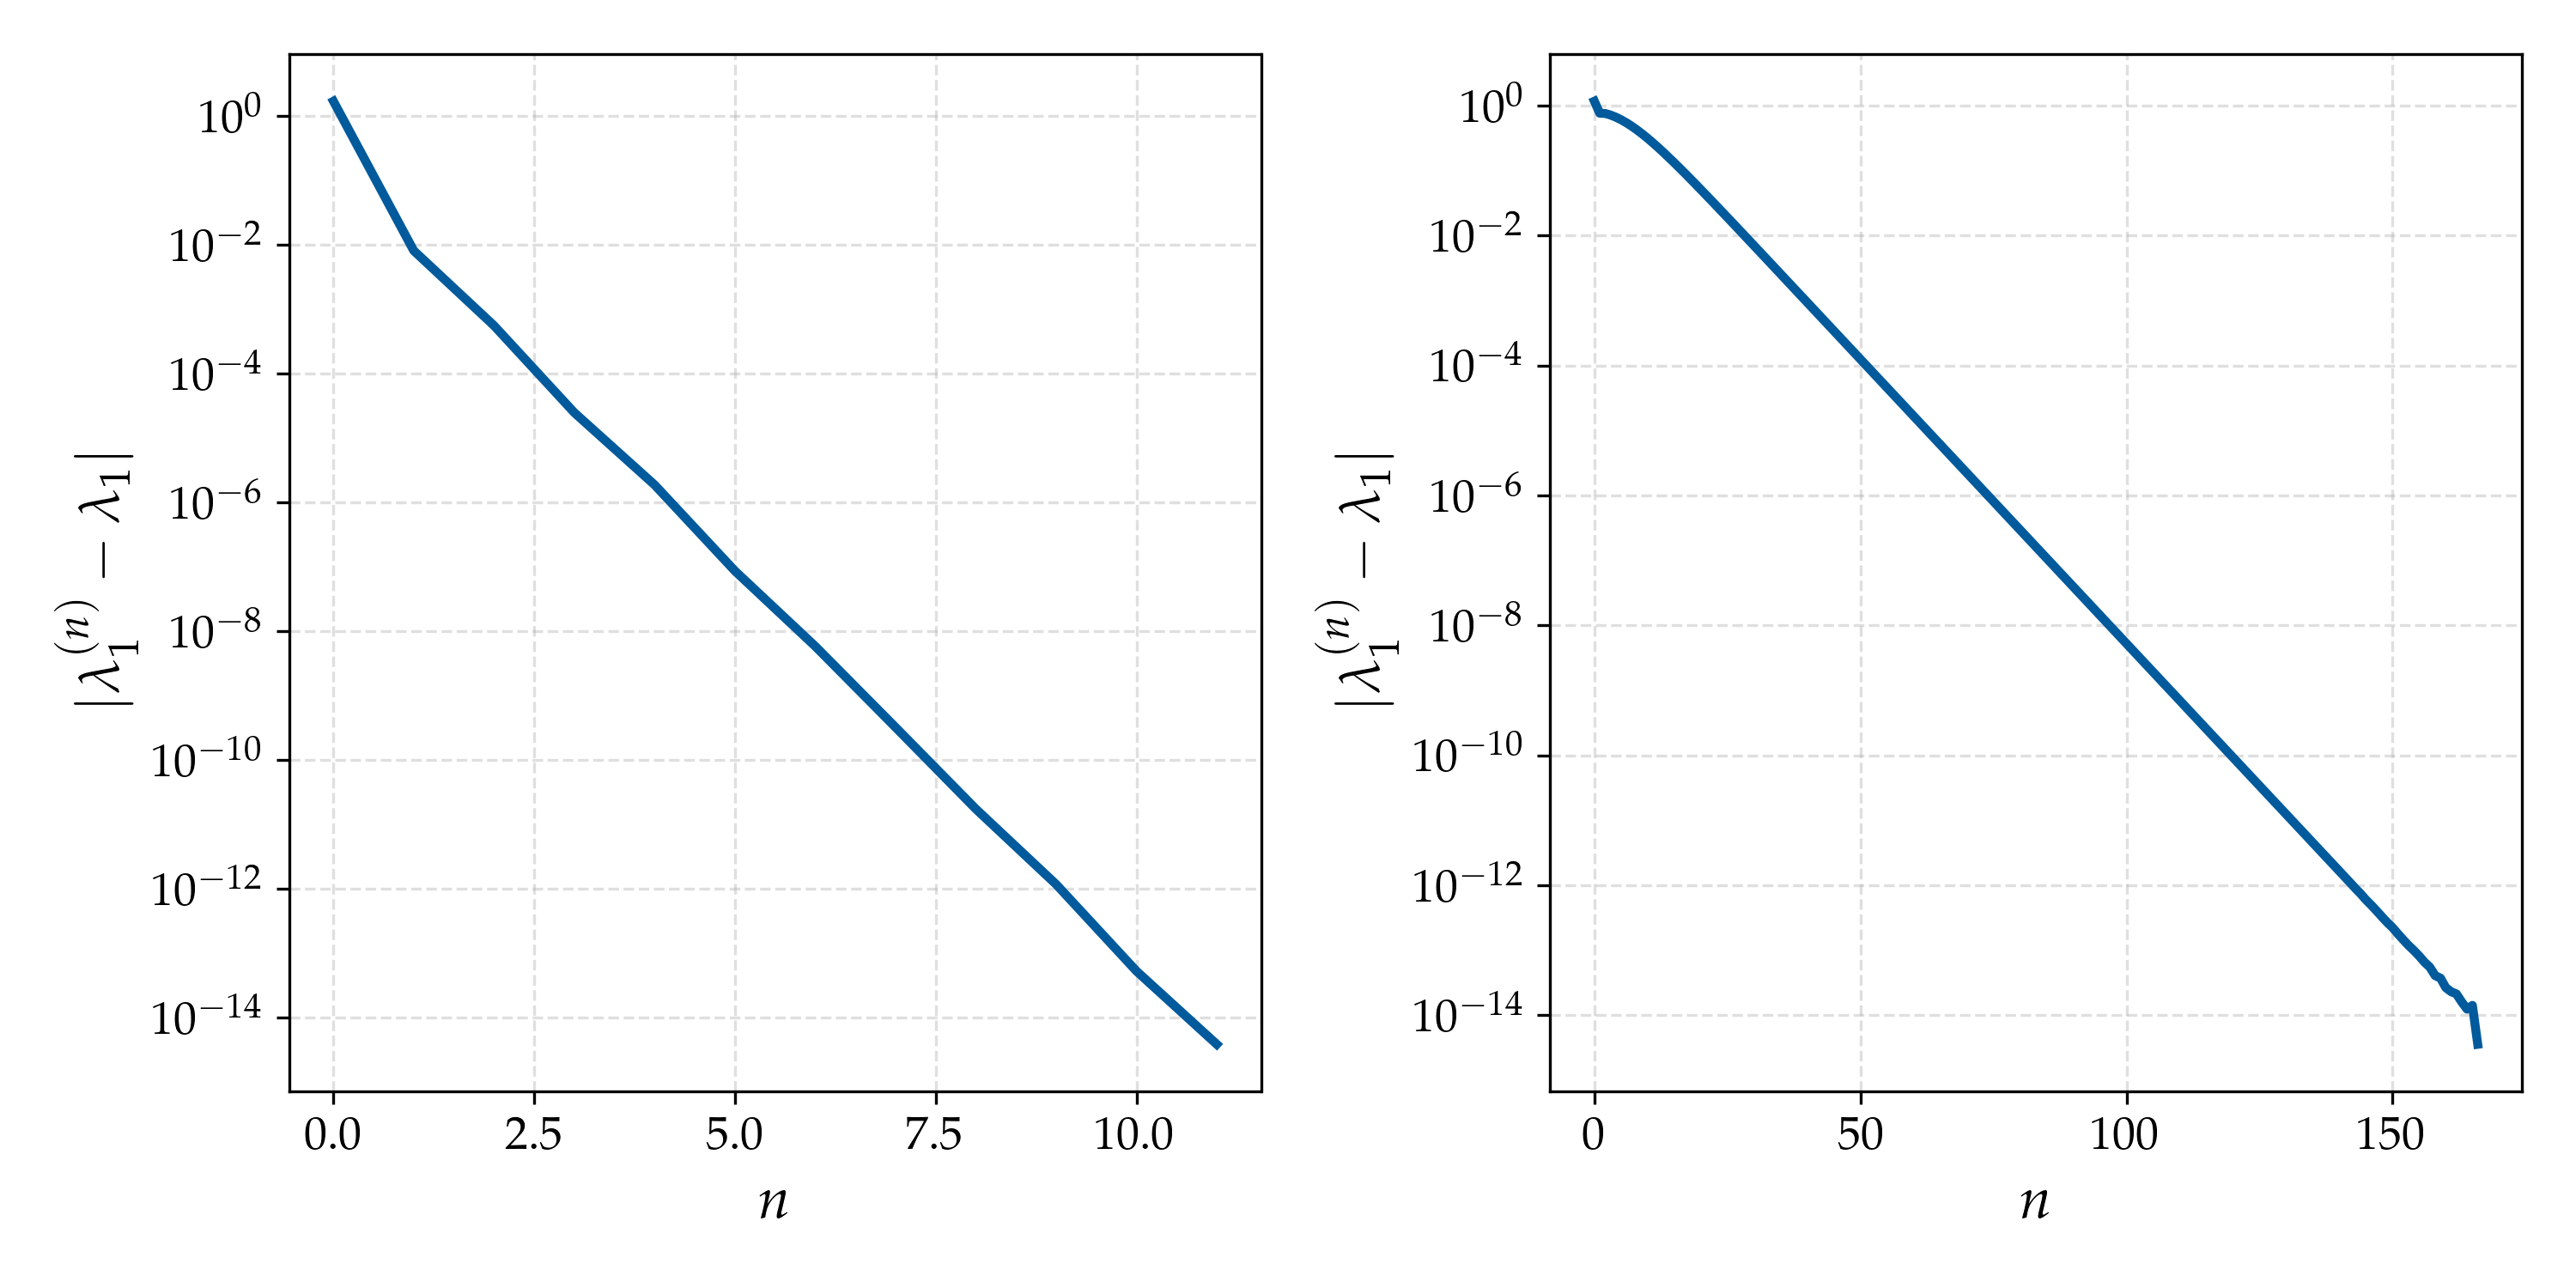
\includegraphics[width=1.1\linewidth]{images/6/plot_powConv.png}
            \caption{Sulla sinistra il caso di $M$, sulla destra $K$. L'andamento della convergenza è lo stesso ma si noti la differenza nel numero di iterazioni necessarie per
            raggiungere la precisione}
            \label{fig: Plot conv Power Mth}
        \end{figure}
    \end{multicols}    

    \item In maniera del tutto simile a quanto fatto in precedenza, e in accordo con ciò che abbiamo descritto nel Cap. \ref{sec: Inverse Pow mth}, risolviamo il problema con questo output:
    \begin{elegantcode}
A =
[[ 4.+0.j -0.-1.j  2.+0.j]
 [ 0.+1.j  2.+0.j  2.+7.j]
 [ 2.+0.j  2.-7.j -2.+0.j]]
 
eig_val_min = (3.1896027470480552-3.51669076861739e-17j)
eig_vect = [ 1.063511 -0.0526563j -0.1124258-0.4313319j -0.2152674-0.0348766j]
    \end{elegantcode}
    
    \item Infine possiamo confrontare i risultati dei due metodi. Gli algoritmi completi sono stati modificati in maniera da restituire la stima dell'autovalore ad ogni step, fino ad un valore fissato di $n=80$ dal quale in poi la precisione dell'\textit{IPM} ha raggiunto la \textit{machine precision} $\varepsilon \approx 10^{-15}$.
    
    
    I valori di confronto per i rapporti ($\lambda_{\text{MAX}}$ e $\lambda_{min}$)sono dati dai punti precedenti dell'esercizio, in cui li abbiamo calcolati esplicitamente. È possibile notare una differenza netta tra la convergenza del primo o del secondo metodo: l'autovalore più piccolo risulta, guardando la matrice inversa, in uno grande, quindi l'effetto dipende dal rapporto tra gli autovalori dell’inversa, cioè $\left|\lambda_{N-1}/\lambda_N\right|$. Ne risulta che l'applicazione della matrice sul vettore random di inizializzazione, ha un effetto più marcato con l'\textit{Inverse}, permettendo una rapida convergenza.

    \begin{figure}[H]
        \centering
        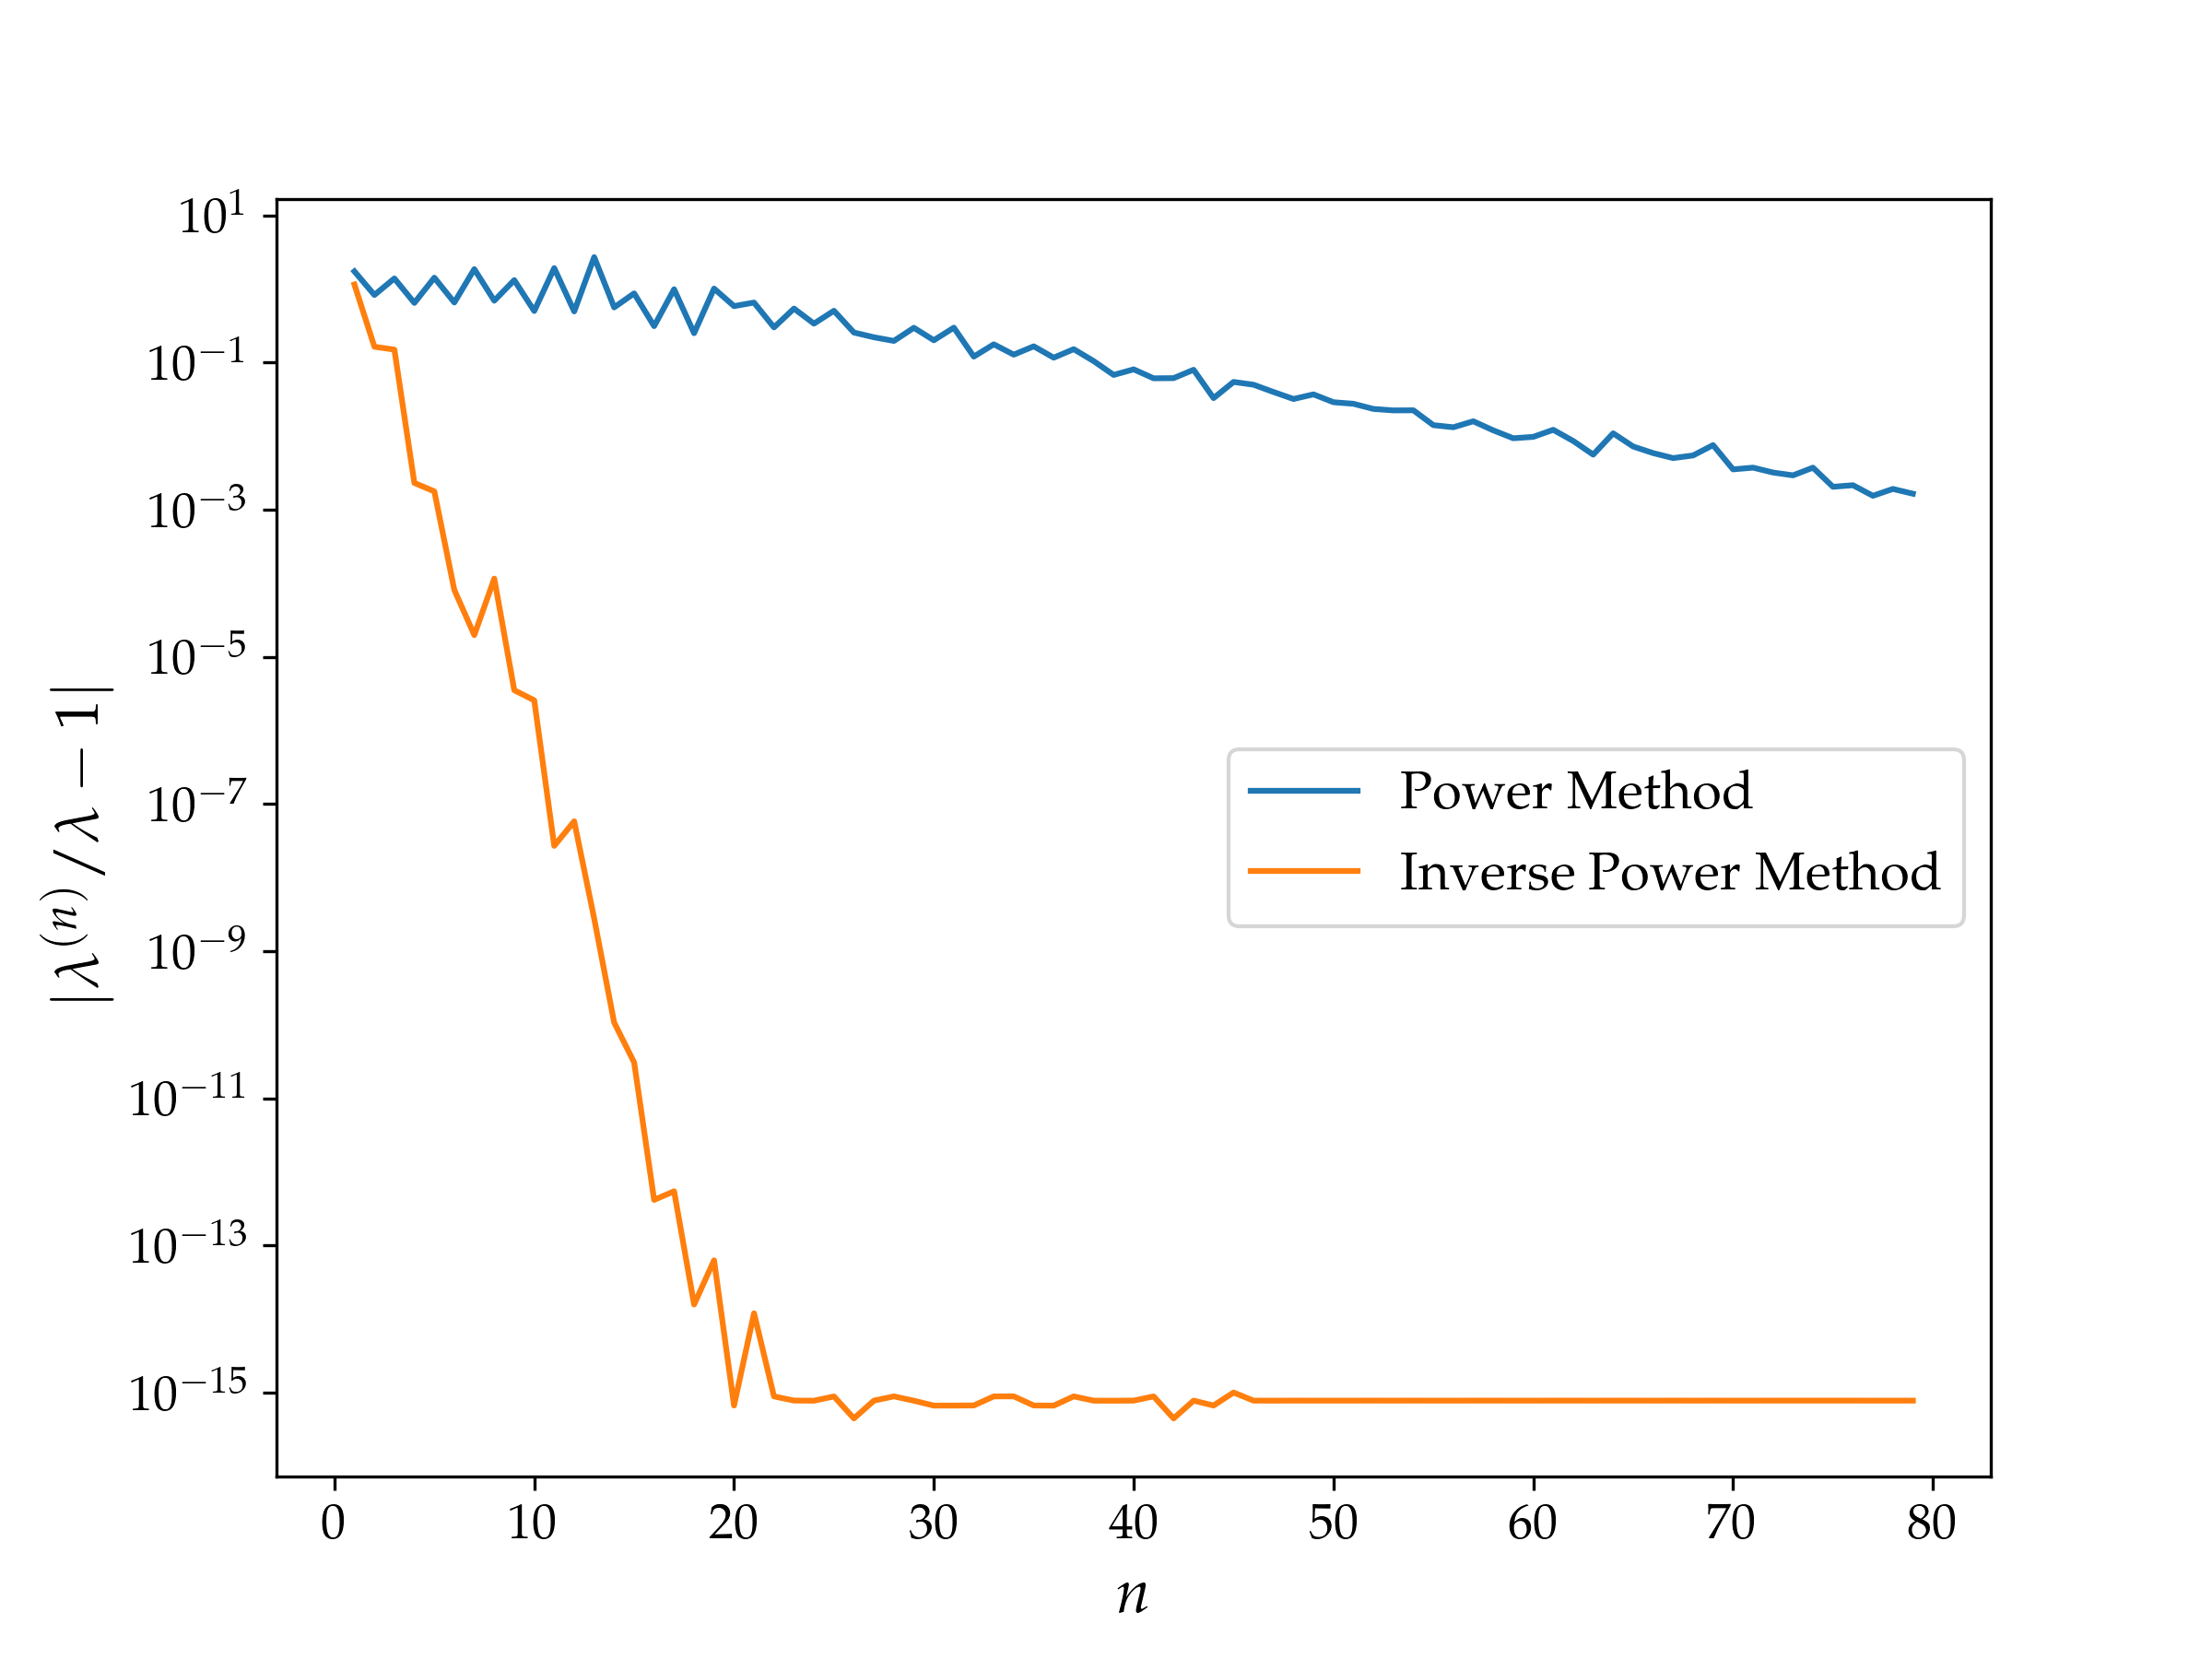
\includegraphics[width=0.7\linewidth]{images/6/pow_vs_inv_convergence.png}
        \caption{Confronto tra il rate di convergenza del \textit{PM} (blu) e quello dell'\textit{IPM} (giallo)}
        \label{fig: Conv Pow vs Inv}
    \end{figure}
\end{enumerate}








\newpage

\section{Esercizio 3.2.1}
\subsection{Problem Statement}
Si implementi una funzione che riceva in ingresso una matrice $A$, una tolleranza $\epsilon$ e un numero massimo di iterazioni $N$. La funzione deve restituire gli autovettori e gli autovalori di $A$ attraverso l'applicazione iterativa della decomposizione $QR$ precedentemente implementata.\\
Poiché si prevede che la matrice risultante $A_\infty$ sia una matrice diagonale (o triangolare superiore a blocchi) contenente gli autovalori lungo la diagonale principale, si definisca un criterio di arresto appropriato. Per testare l'algoritmo, si utilizzi la matrice tridiagonale che rappresenta l'operatore Laplaciano unidimensionale, considerando dimensioni modeste dell'ordine di $O(10)$.\\
Si produca infine un grafico che mostri l'andamento della convergenza per ogni singolo autovalore in funzione del numero di iterazioni.

\subsection{Premessa Teorica}
Una possibilità per lo sviluppo di un algoritmo di estrazione degli autovalori di una matrice sta nei metodi di decomposizione della matrice di test $A$: se è effettivamente possibile implementare un algoritmo che faccia uso della Decomposizione LU, è molto più conveniente lo sviluppo di uno che usi la Decomposizione QR, più stabile e possibile per una qualsiasi matrice generica. Questo rappresenta un metodo di algoritmo iterativo, portandosi dietro tutte le sue potenzialità, ma anche le sue problematiche.

\subsection{Metodi Numerici e Algoritmi}
Si procede definendo iterativamente $A_k$, fissando $A_0 = A$: da qui in poi, potendo decomporre con \textit{QR decomposition}, quindi $A_k = Q_kR_k$, si definisce la matrice al passo $k+1$ come $A_{k+1}=R_kQ_k$. Questa operazione è una trasformazione di similitudine, infatti si può mostrare che $A_{k+1}=Q^\dagger_k A_k Q_k$, e la sua importanza sta nel fatto di conservare lo spettro della matrice originale.\\
Per un numero grande di iterazioni:
\begin{enumerate}
    \item $A_k$ converge verso $A_\infty$, che è la sua diagonalizzata, cioè presenta gli autovalori sulla diagonale e zeri nel resto.
    \item $\prod_{j=0}^k Q_j$, converge a $Q_\infty$, le cui colonne sono gli autovettori che costituiscono una base ortonormale di $A$.
\end{enumerate}
Queste conclusioni sono valide nella maniera qui esposta solo per matrici hermitiane, per una matrice generica $A_\infty$ è triangolare superiore e l'algoritmo si complica. Ci limitiamo quindi a studiare matrici hermitiane, che sono una classe abbastanza rappresentativa per i problemi di fisica che andremo ad analizzare.

\subsection{Risultati e Discussione}
Il test sulla ricerca degli autovalori viene fatto su una matrice $A \in \mathbb{C}^{3 \times 3}$ (hermitiana), definita come segue:
\begin{elegantcode}
ndim = 3
re = np.random.rand(ndim, ndim)
im = np.random.rand(ndim, ndim)
Z = re + 1j * im
A_test = (Z + Z.T.conj()) / 2       # per assicurare A hermitiana
\end{elegantcode}
\noindent L'algoritmo ha il criterio di fermarsi quando smette di vedere una evoluzione nei valori di $A_k$, definito così in codice \textit{.py}

\begin{elegantcode}
if np.sqrt(np.sum(np.abs(Ak - np.diag(np.diag(Ak)))**2)) < tol:
    print(f'Tolerance reached at step {i+1}')
    eigenVal = np.diag(Ak)
    eigenVect = Qk
    return eigenVal, eigenVect
\end{elegantcode}
Il risultato, comprensivo della matrice di test, è espresso nella cella qui sotto:

\begin{elegantcode}
Tolerance reached at step 35

A =
 [[0.56820981+0.j         0.9532166 -0.05799793j 0.47756225-0.09283526j]
 [0.9532166 +0.05799793j 0.30847352+0.j         0.45485252+0.04791834j]
 [0.47756225+0.09283526j 0.45485252-0.04791834j 0.15548257+0.j        ]]

eig_val = [ 1.68903863+1.1017535e-17j -0.53975861-5.9673907e-18j
 -0.11711411+7.2000436e-18j]

eig_vect = [[ 0.68845441-1.24812738e-17j -0.63535769-1.71610507e-02j
  -0.34150506-7.36947240e-02j]
 [ 0.60423579+5.55867258e-02j  0.75235531-2.10953753e-02j
  -0.21152465+1.43467835e-01j]
 [ 0.39534364+3.92829679e-02j -0.05662805+1.62283202e-01j
   0.90091426-3.11635707e-02j]]
\end{elegantcode}
\noindent È possibile verificare che questo risultato è corretto con le stesse modalità espresse nel Cap.\ref{sec: Controllo autovalori}, quindi come segue:
\begin{elegantcode}
if not np.allclose(A_in @ eigenVect, eigenVal * eigenVect, rtol=tol):
    raise ValueError('Eigenpair not accurate')
\end{elegantcode}
\medskip
\noindent Come richiesto dall'esercizio, possiamo svolgere per la matrice tridiagonale che rappresenta il Laplaciano unidimensionale, $K \in \mathbb{Z}^{10\times 10}$, valutando lo spettro.
Diventa molto interessante la figura ottenibile dalla visualizzazione dell'errore in funzione dei singoli autovalori, cioè l'andamento della convergenza per diversi valori di $\lambda$ (Fig. \ref{fig: Conv sing eigen}).

\begin{figure}[H]
    \centering
    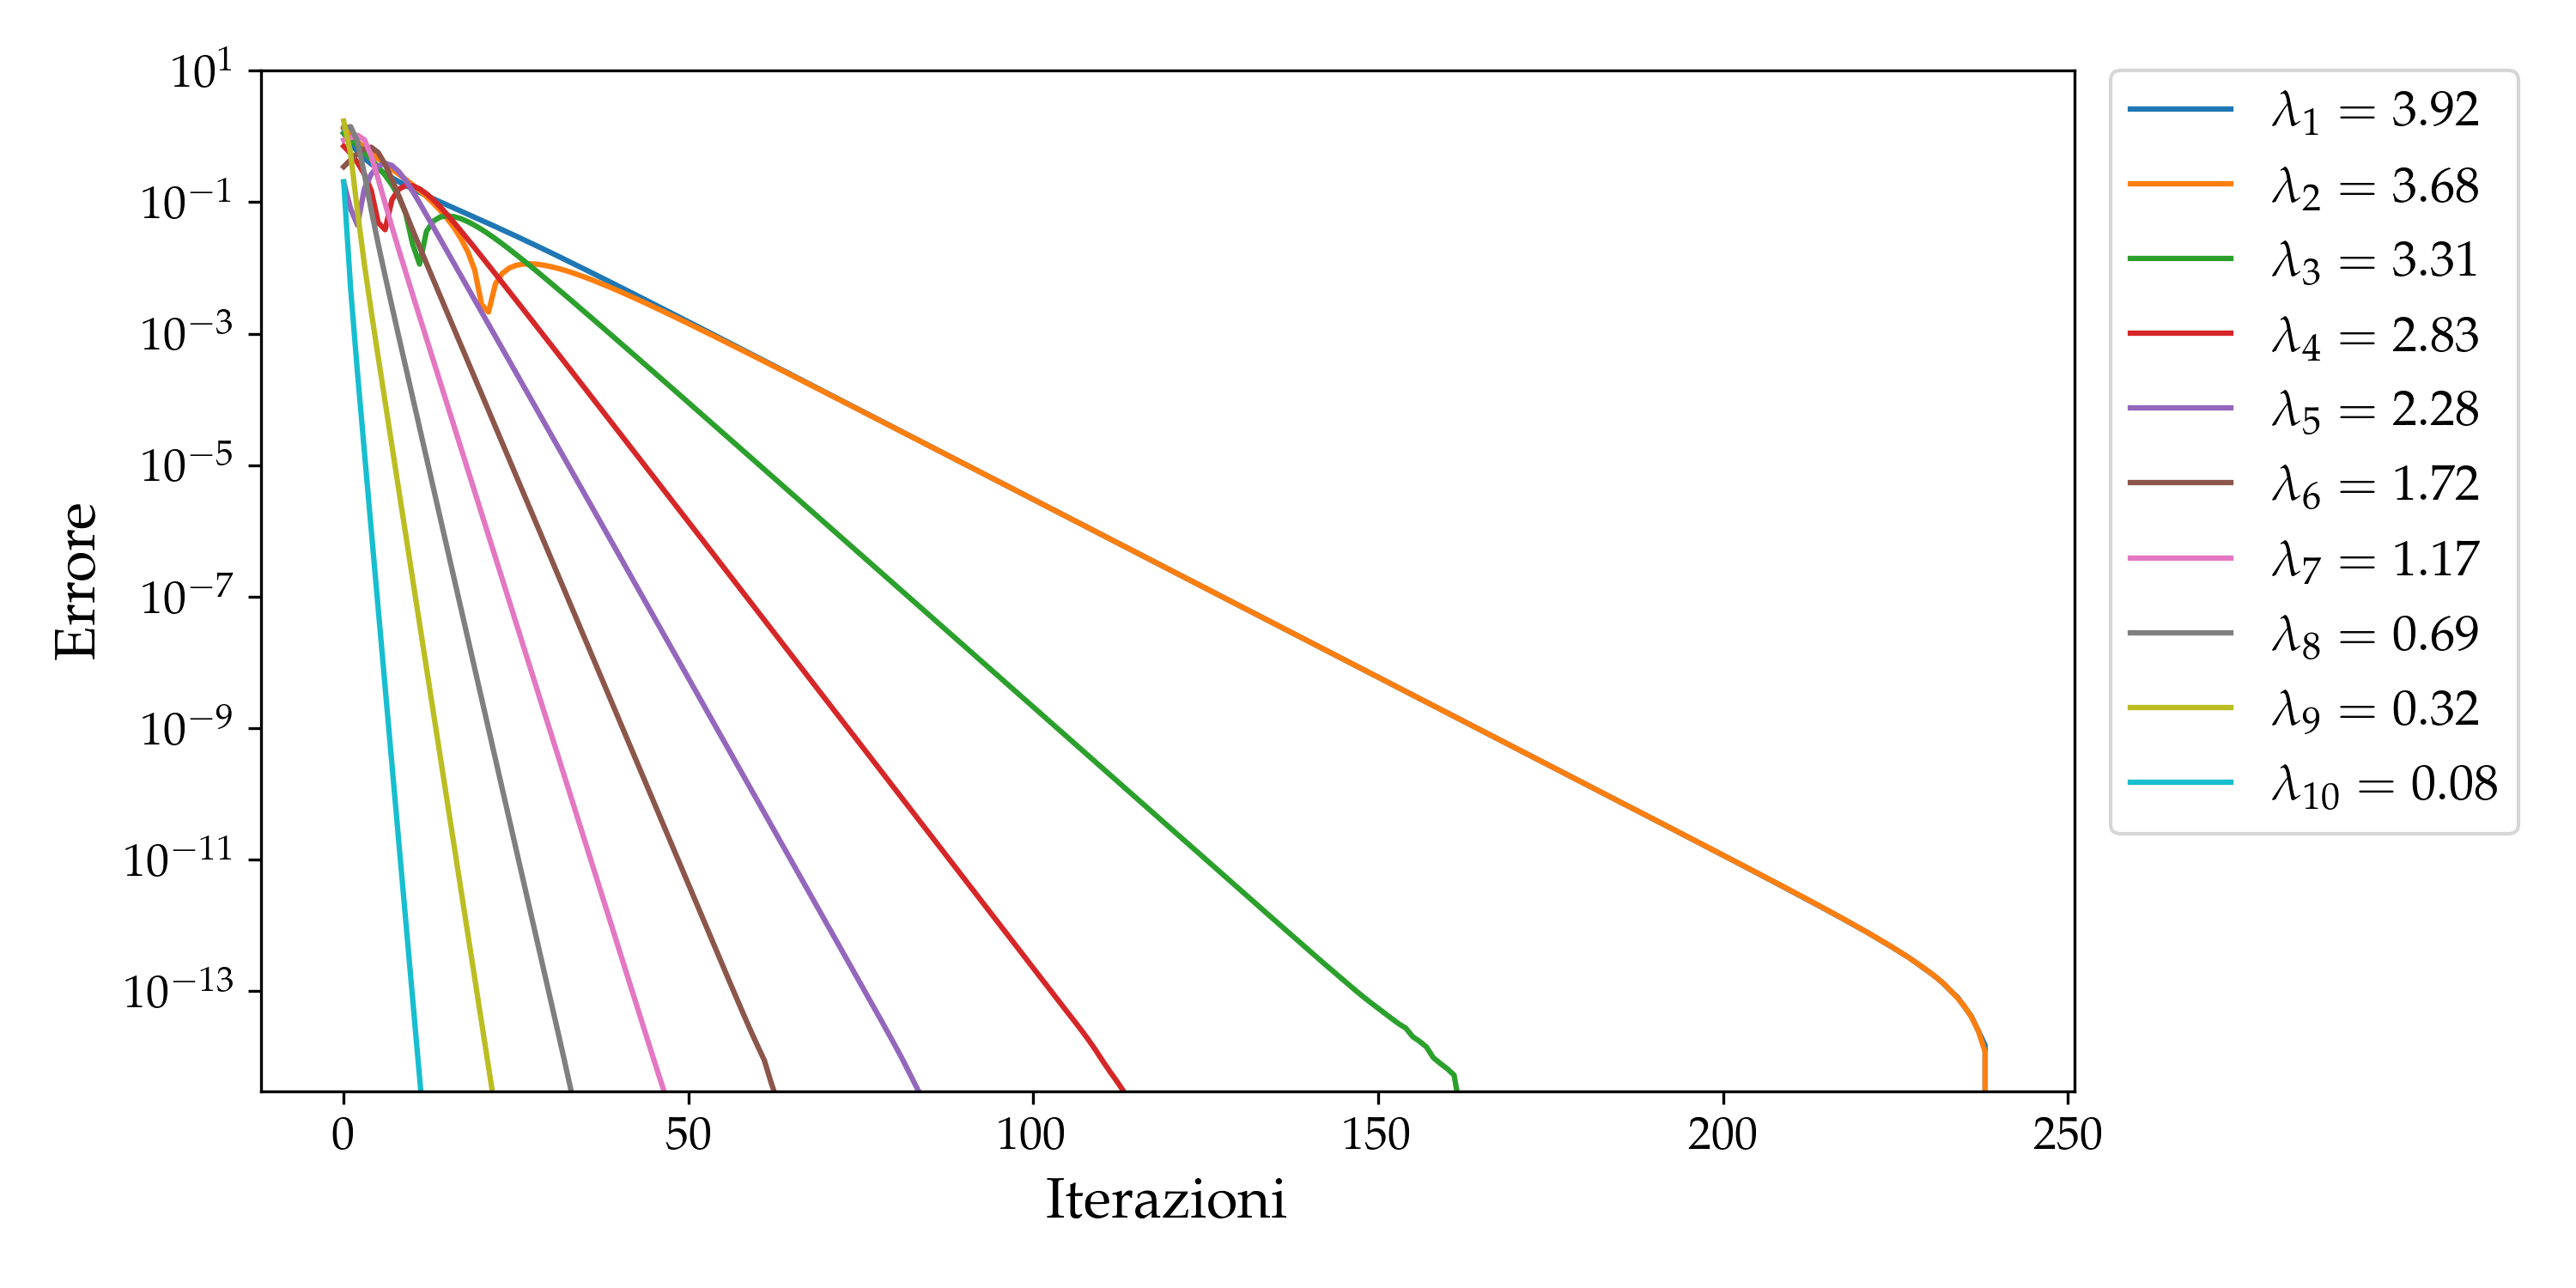
\includegraphics[width=0.7\linewidth]{images/7/conv_single_eigen.png}
    \caption{Andamento della convergenza per diversi autovalori di $K$.}
    \label{fig: Conv sing eigen}
\end{figure}



% --- PARTE 4: Interpolazione e Fitting ---
\cleardoublepage 
\addtocontents{toc}{\bigskip\noindent\protect\textbf{\Large Interpolazione e Fitting}\par\smallskip}
\addtocontents{toc}{\protect\setcounter{tocdepth}{-2}} 
\part{\Huge Interpolazione e Fitting}
\addtocontents{toc}{\protect\setcounter{tocdepth}{2}} 

\section{Esercizio 4.1.1}

\subsection{Problem Statement}
Scrivi un programma che esegua la \textbf{Lagrange interpolation}. In questo caso, poiché i pesi sono precomputati, è particolarmente utile costruire una classe che li memorizzi internamente.

\begin{elegantcode}[title=Schema della classe Lagrange]
class Lagrange:
    property weights = calcolati quando la class viene inizializzata
    
    method eval = restituisce la interpolation alla posizione x
\end{elegantcode}

Testa la funzione sui seguenti set di dati:
\begin{enumerate}
    \item Dataset A
    \begin{elegantcode}
xA = np.array([0, 2, 3, 5, 7, 8, 10])
fA = np.array([0, 2, 2.5, 4, 2.5, 2, 0])
    \end{elegantcode}
    
    \item Dataset B
    \begin{elegantcode}
xB = np.array([0, 2, 3, 4, 5, 6, 7, 8, 10])
fB = np.array([0, 2, 2.5, 2, 4, 2, 2.5, 2, 0])
    \end{elegantcode}
    
    \item Dataset C
    \begin{elegantcode}
xC = np.array([0, 1, 2, 3, 4, 5, 6, 7, 8, 9, 10])
fC = np.array([0, 1.5, 2, 2.5, 2, 4, 2, 2.5, 2, 1.5, 0])
    \end{elegantcode}
\end{enumerate}

\subsection{Premessa Teorica}
Il problema che ci siamo posti è quello di trovare una curva che passi esattamente per dei punti fissati dalla richiesta, ricostruire quindi una forma analitica che ammetta per la controimmagine $\boldsymbol{x}$, immagine $\boldsymbol f$. Possiamo scegliere diversi tipi di interpolazioni, ci concentriamo su quelle lineari, cioè ricerchiamo:
\[
P(x) = \sum a_k\ \phi_k(x)\ , \quad P(x_i) = f_i\
\]

\noindent In particolare per una interpolazione Polinomiale:
\[
\phi_k(x) = x^k
\]

\subsection{Metodi Numerici e Algoritmi}

\subsubsection{Direct Method} \label{Cap: Direct Mth}
Il primo tentativo di interpolare dei punti con una curva può essere fatto implementando il cosiddetto \textit{Direct Method}: dato un set di $n$ punti $(x_i, f_i)$ si può introdurre una matrice $n\times n$ $V$ tale che
\[
f=aV
\]

\noindent scegliendo la base dei monomi $V$ è detta \textit{Matrice di Vandermonde}, così definita:
\[
V = \begin{pmatrix}
1 & x_1 & x_1^2 & \dots \\
1 & x_2 & x_2^2 & \dots \\
\dots
\end{pmatrix}
\]
A questo punto la ricerca del vettore dei coefficienti diventa la semplice risoluzione di un sistema lineare con la martice $V$, risolvibile agilmente con uno dei metodi che abbiamo precedentemente mostrato (Parte \ref{Cap: Matrici e Sistemi Lineari}).\\ 
\noindent Questa non risulta essere una buona soluzione alla ricerca del polinomio interpolante il sistema di punti generico, poiché si può dimostrare che al crescere del sistema la matrice diventa sempre più mal-condizionata. Un plot di seguito (Fig. \ref{fig: Vandermonde cond}) mostra il \textit{Condition Number} di $V$ in funzione del numero di punti da interpolare, che dimostra ciò a cui abbiamo appena fatto riferimento. 

\begin{figure}[H]
    \centering
    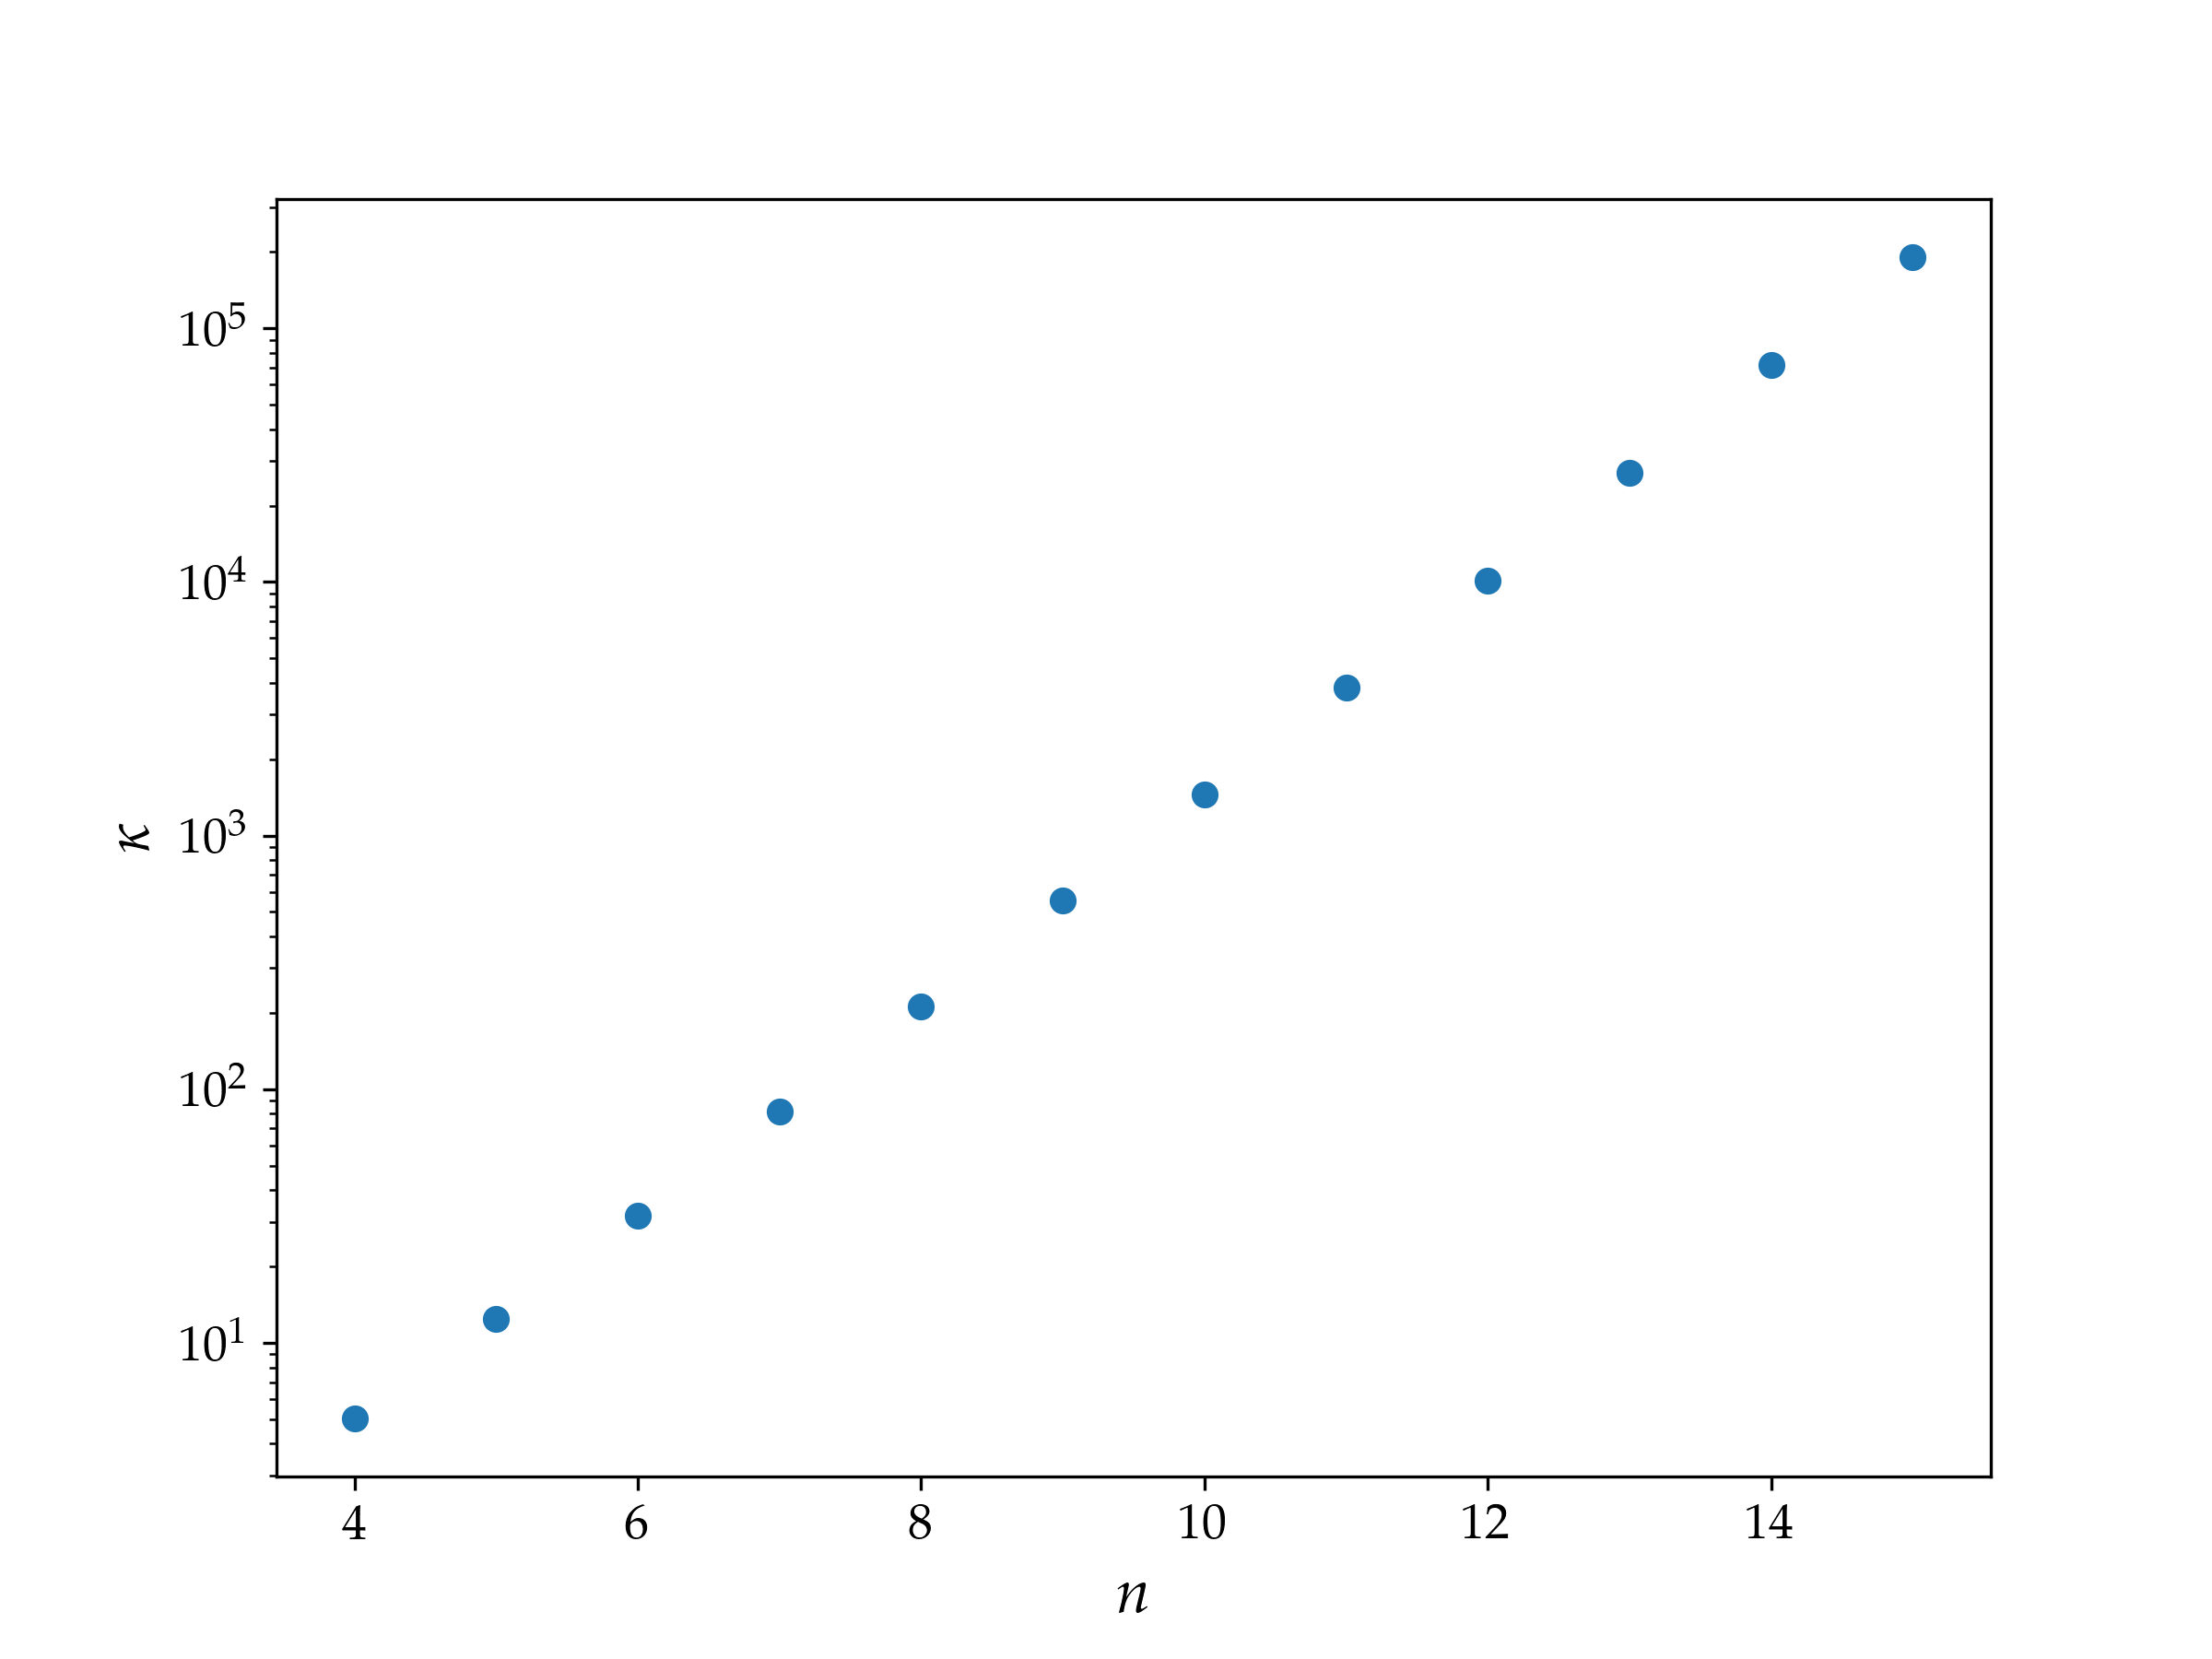
\includegraphics[width=0.7\linewidth]{images/8/Vandermonde_cond.png}
    \caption{\textit{Condition number} $\kappa$ della matrice di Vandermonde in funzione del numero di punti da interpolare $n$.}
    \label{fig: Vandermonde cond}
\end{figure}

\subsubsection{Lagrange Interpolation}
Un'alternativa è proposta dall'interpolazione di Lagrange, dove definiamo i \textit{Polinomi di Lagrange} $L_k(x)$:
\[
L_k(x) = \frac{\prod_{j=0, j \neq k}^{n-1}(x - x_j)}{\prod_{j=0, j \neq k}^{n-1}(x_k - x_j)} = w_k \prod_{j=0, j \neq k}^{n-1}(x - x_j)\
\]
\[
\frac{1}{w_k} = \prod_{j=0, j \neq k}^{n-1}(x_k - x_j) \quad \text{è una costante}
\]
La caratteristica principale di $L_k(x)$ è quella che 
\[
L_k(x_i) = \delta_{ki}
\]
quindi segue:
\[
P(x) = f = \sum a_k\ L_k(x) = \sum a_k \delta_{ki} = a_i
\]
Cioè la matrice di Vandermonde è l'identità, e non è necessario risolvere il sistema lineare poiché è banale. \\
Una riscrittura è possibile per ottimizzare il costo computazionale del problema:
\[
\begin{aligned}
P(x) = \dots = \left[ \sum_{k} \frac{f_k w_k}{(x - x_k)} \right] \left[ \sum_{k} \frac{w_k}{(x - x_k)} \right]^{-1}
\end{aligned}
\]

\noindent Si noti che nel calcolo del polinomio esattamente su un nodo si potrebbero incontrare problemi di divergenza del risultato numerico: risolviamo introducendo una piccola deviazione $\epsilon$, dell'ordine della \textit{machine precision}, trascurabile nel calcolo ordinario, ma che assicura alla nostra computazione, in questi casi più delicati, di non fallire

\[
\begin{aligned}
P(x) = \dots = \left[ \sum_{k} \frac{f_k w_k}{(x - x_k + \epsilon)} \right] \left[ \sum_{k} \frac{w_k}{(x - x_k + \epsilon)} \right]^{-1}
\end{aligned}
\]

\subsection{Risultati e Discussione}
L'uso di una classe risulta naturale, infatti il calcolo dei pesi è un'operazione da fare una sola volta, dato un certo set di punti, quindi essi possono essere computati e conservati.\\
Ho implementato questo tipo di logica nella mia soluzione:
\begin{elegantcode}
class Lagrange:
    def __init__(self, x, f):
        self.x = x
        self.f = f
        n = len(x)
        w_arr = []
        for k in range(n):
            mask = np.ones(len(x), dtype=bool)
            mask[k] = False
            wk = np.prod((x[k] - x[mask] + 1e-15))**(-1)
            w_arr.append(wk)
        self.w = np.array(w_arr)

    ...
\end{elegantcode}
\bigskip
\noindent Sono forniti 3 \textit{dataset}, vengono mostrati di seguito i punti nel piano (Fig \ref{fig: Repr dataset}) e la loro interpolazione con una curva, tramite metodo dei Polinomi di Lagrange (Fig \ref{fig: Lagrange interp}).

\begin{figure}[H]
    \centering
    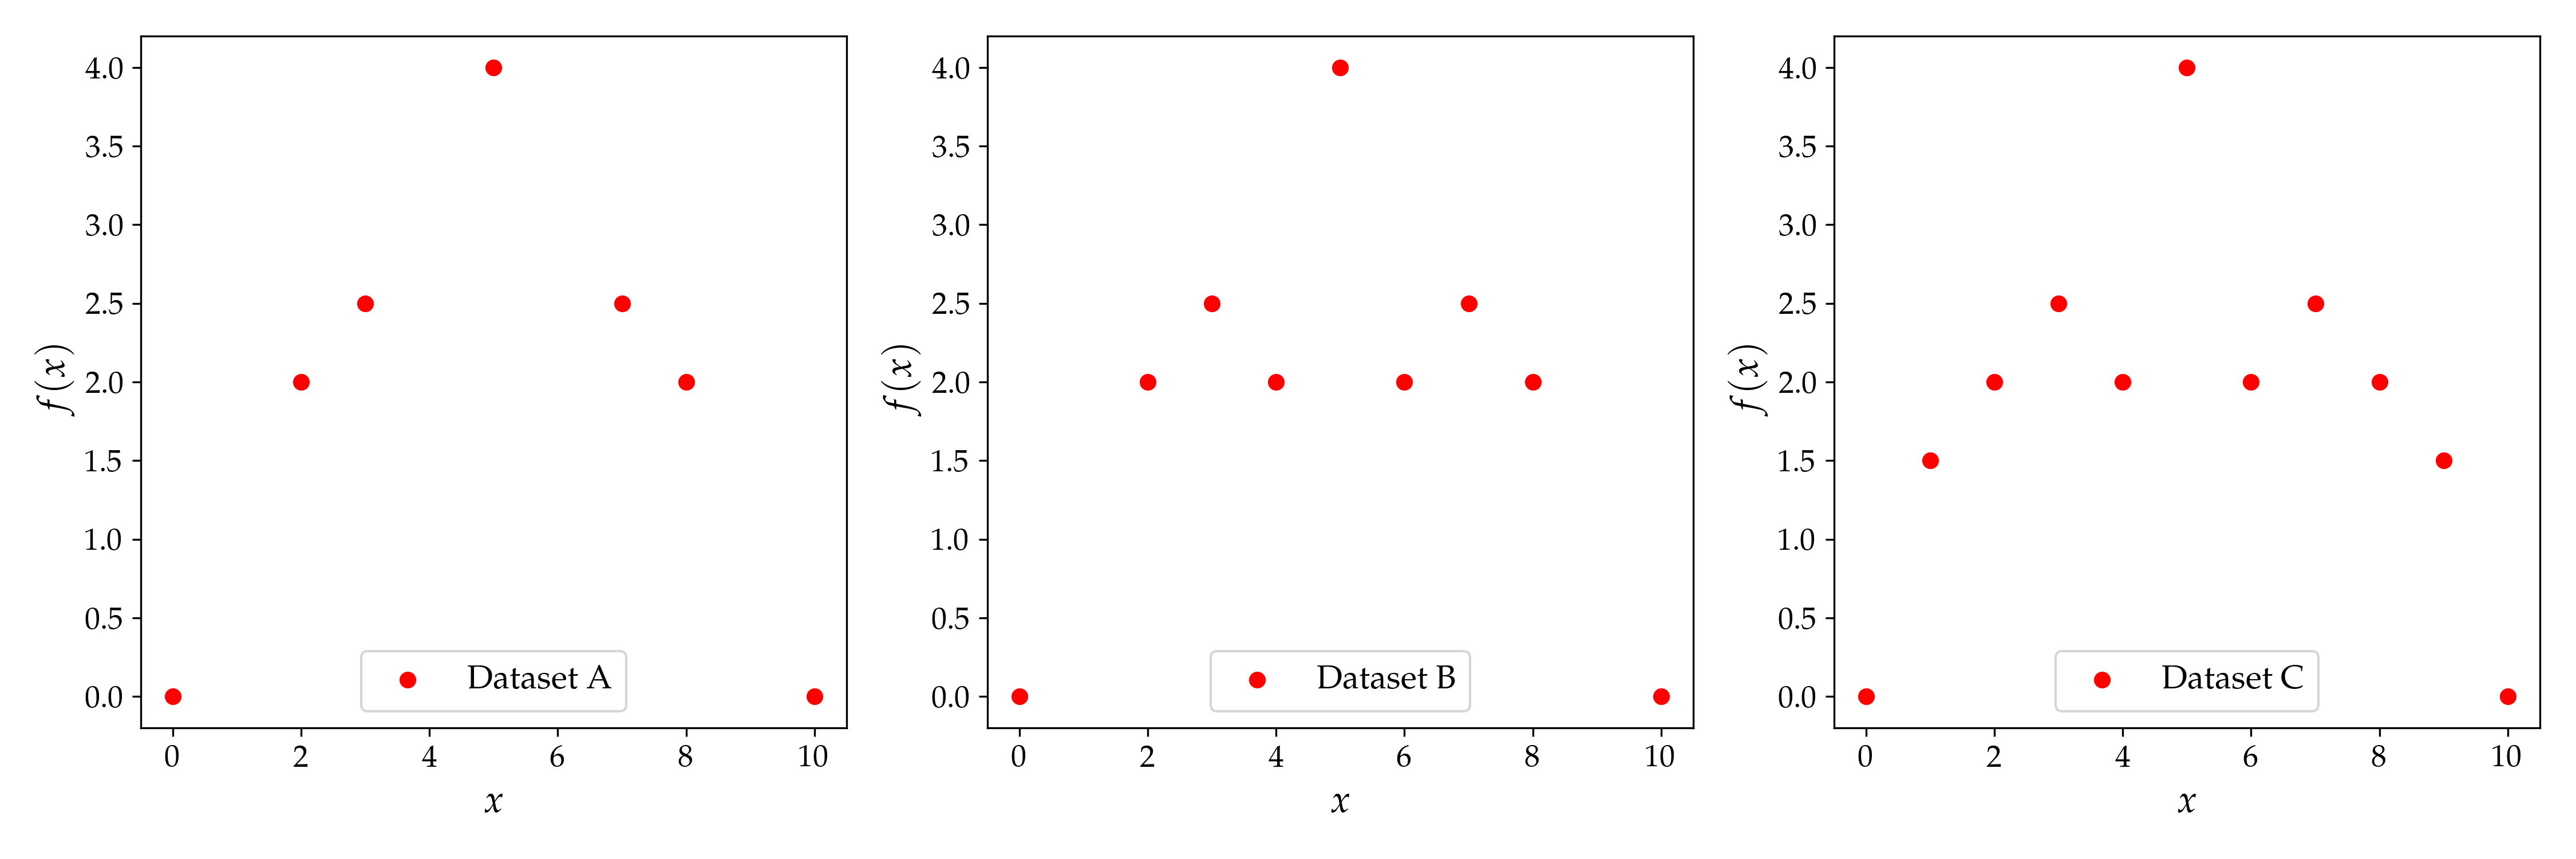
\includegraphics[width=\linewidth]{images/8/Lagrange_dataset_plot.png}
    \caption{Rappresentazione dei dataset.}
    \label{fig: Repr dataset}
\end{figure}

\begin{figure}[H]
    \centering
    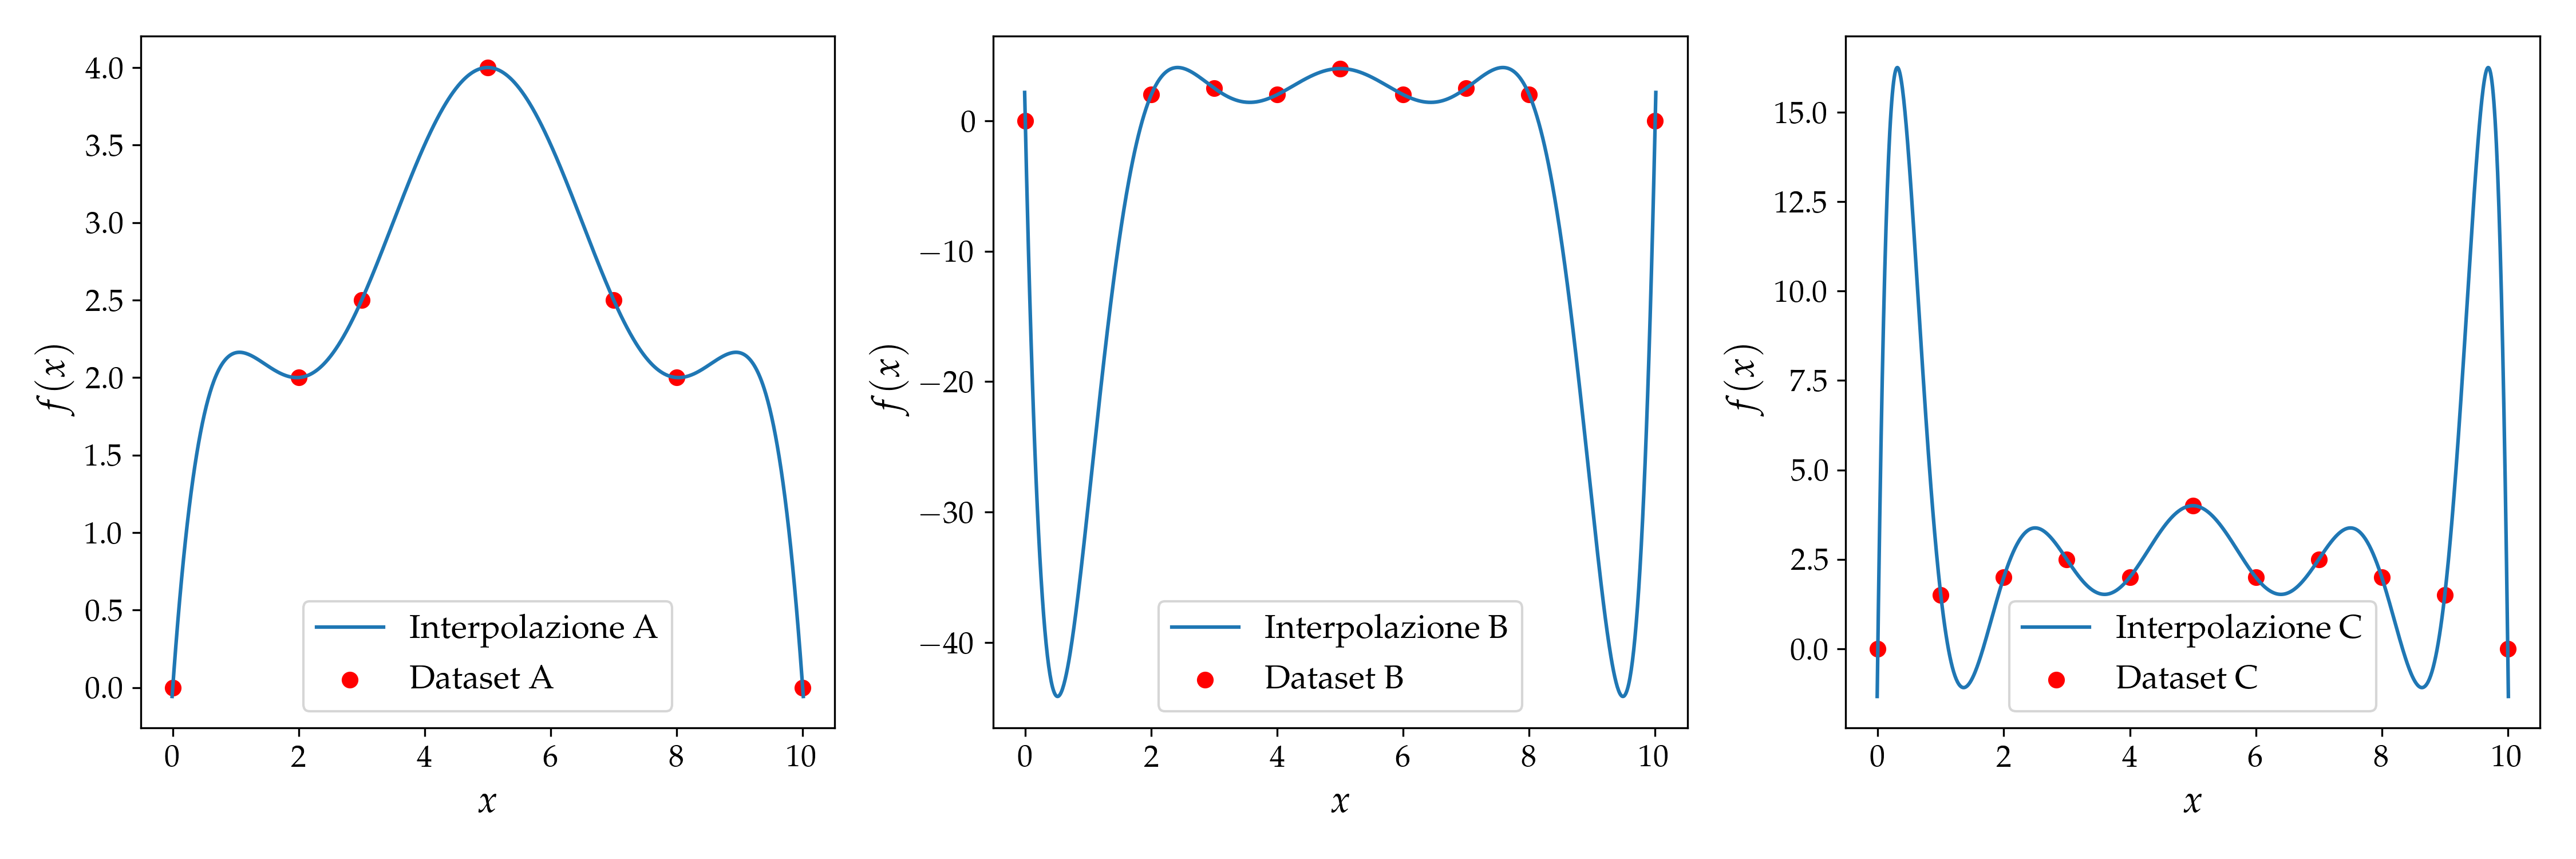
\includegraphics[width=\linewidth]{images/8/Lagrange_Interpolation.png}
    \caption{Interpolazione con \textit{Lagrange}.}
    \label{fig: Lagrange interp}
\end{figure}

\bigskip
\noindent Risulta interessante il confronto con l'interpolazione della curva tramite il \textit{Direct Method}. I problemi principali di questo approccio sono stati presentati nel Cap. \ref{Cap: Direct Mth}, ma qui vogliamo analizzare i risultati diretti di questa implementazione.

Nella Fig. \ref{fig: Dir mth interp} vediamo rappresentata la forma funzionale, polinomiale, trovata da questo secondo metodo e risulta evidente la similitudine con Fig. \ref{fig: Lagrange interp}.
\begin{figure}[H]
    \centering
    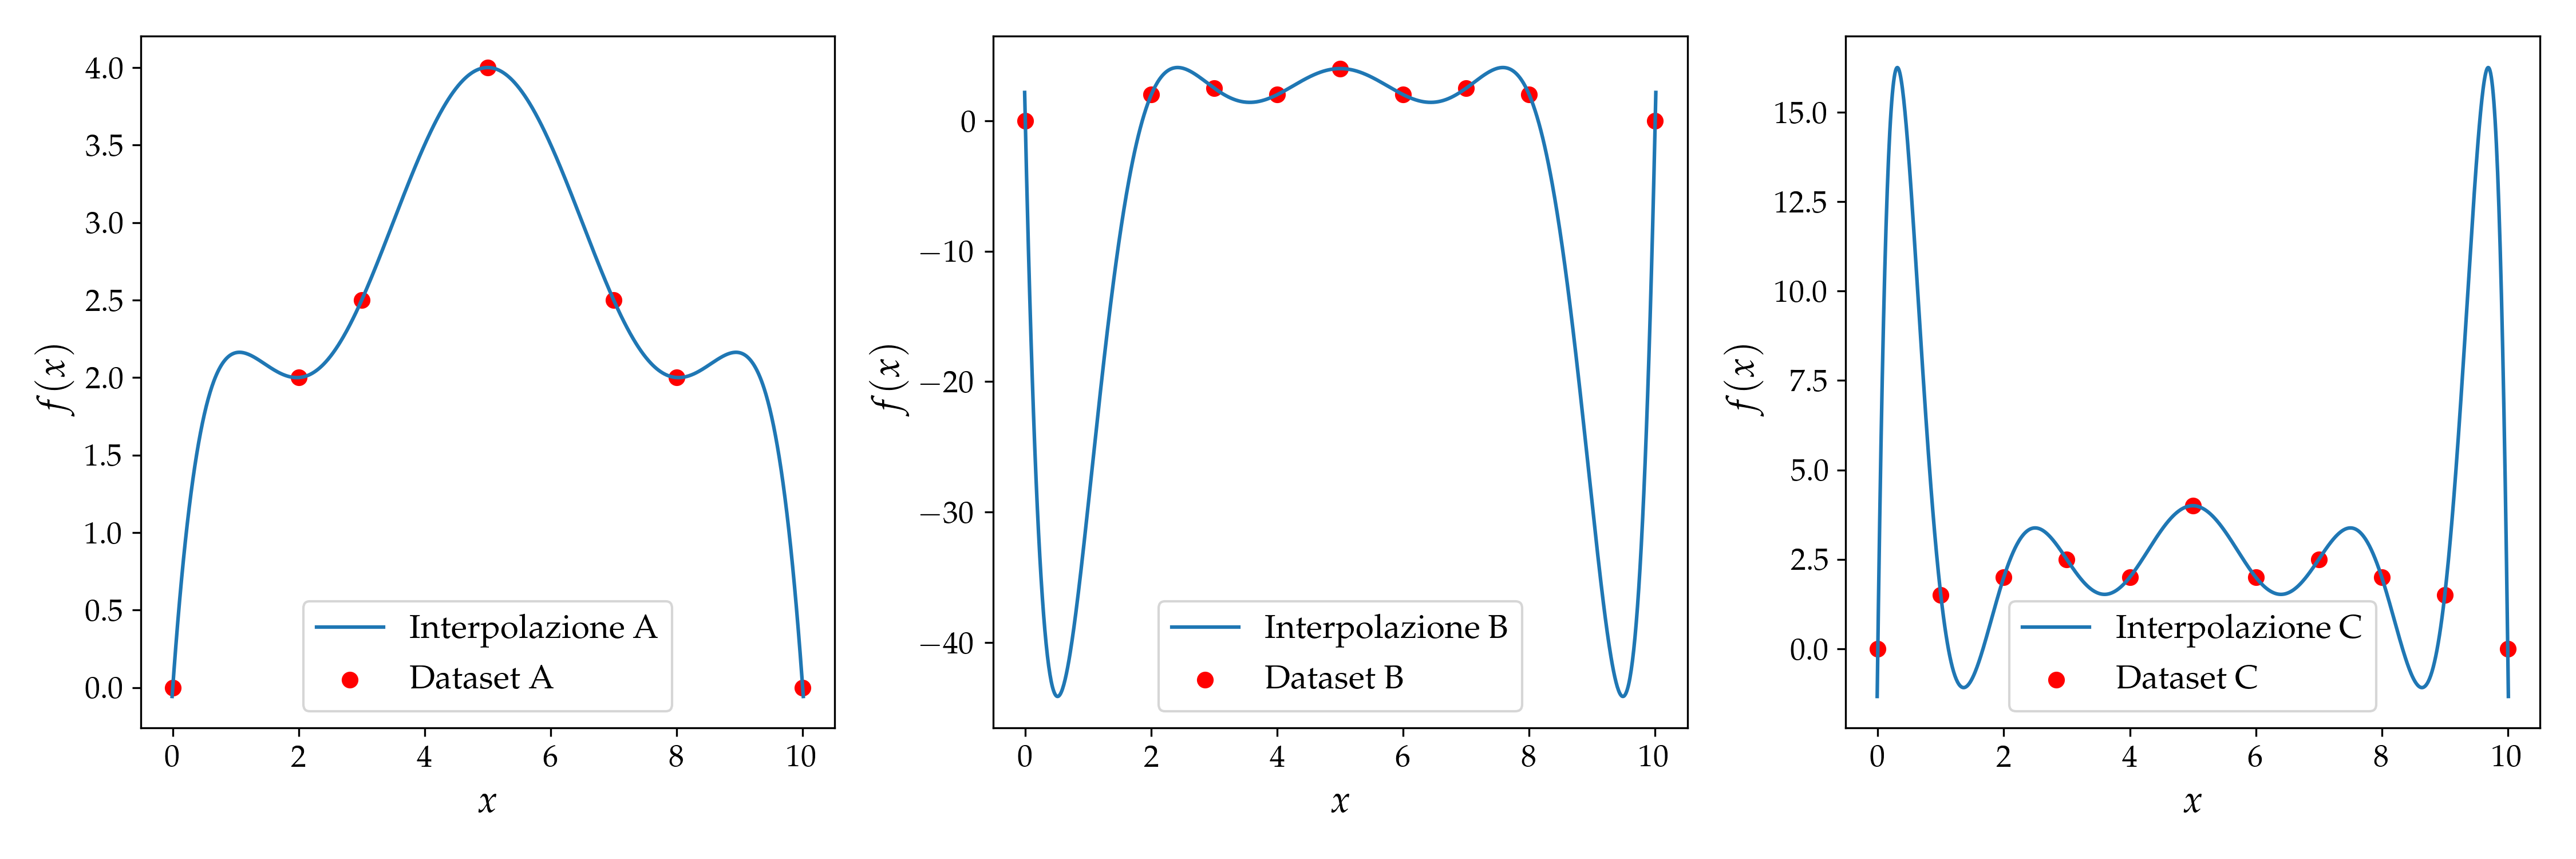
\includegraphics[width=\linewidth]{images/8/Direct_mth.png}
    \caption{Interpolazione con \textit{Direct Method}.}
    \label{fig: Dir mth interp}
\end{figure}

\noindent Una anlisi più precisa del fenomeno è possibile osservando l'errore assoluto tra le due descrizioni, definito come $|f_L(x) - f_D(x)|= E(x)$. Con riferimento al plot in Fig. \ref{fig: Err dir vs lag}, possiamo descrivere due andamenti differenti: se in prima analisi si osserva empiricamente una correlazione qualitativa tra l’andamento dell’errore e quello della funzione (ma senza una relazione generale), esiste un secondo \textit{slope} più interessante e preponderante nella parte destra del grafico. 

\medskip
\noindent Si osserva che $E(x)$ passa da un andamento regolare e ben definito a uno caratterizzato da oscillazioni sempre più pronunciate. Inoltre, l’ordine di grandezza dell’errore aumenta all’aumentare del numero di punti, mostrando una crescita approssimativamente esponenziale.

La spiegazione per queste osservazioni viene trovata nel mal condizionamento della \textit{Matrice di Vandermonde} e nel \textit{Direct Method}. Abbiamo mostrato già nel Cap.\ref{Cap: Direct Mth} come al crescesere del numero di punti, aumenti $\kappa$ per $V$, e questo spiega i diversi ordini di grandezza visibili sulla scala degli errori per i differenti dataset. 

Per quanto riguarda le oscillazioni della funzione, è necessario ricondursi alla definizione della matrice $V$, che contiene, nelle ultime colonne, termini dell'ordine di $x_i^N$, con $N$ numero di punti. Per N grande vengono molto amplificati gli errori sui coefficienti (instabilità numerica), inoltre le combinazioni di potenze con coefficienti di segno opposto porteranno a somme algebriche di numeri con diversi ordini di grandezza di differenza: questo lascia la possibilità per errori di arrotondamento legati alla \textit{machine precision}.

\medskip
\noindent Infine si può notare come spesso i minimi dell'errore si trovino in corrispondenza dei nodi, cioè dei punti in cui fissiamo il valore della funzione in maniera più rigida: le due interpolazioni saranno tendenzialmente più concordi sui valori qui assegnati.

\begin{figure}[H]
    \centering
    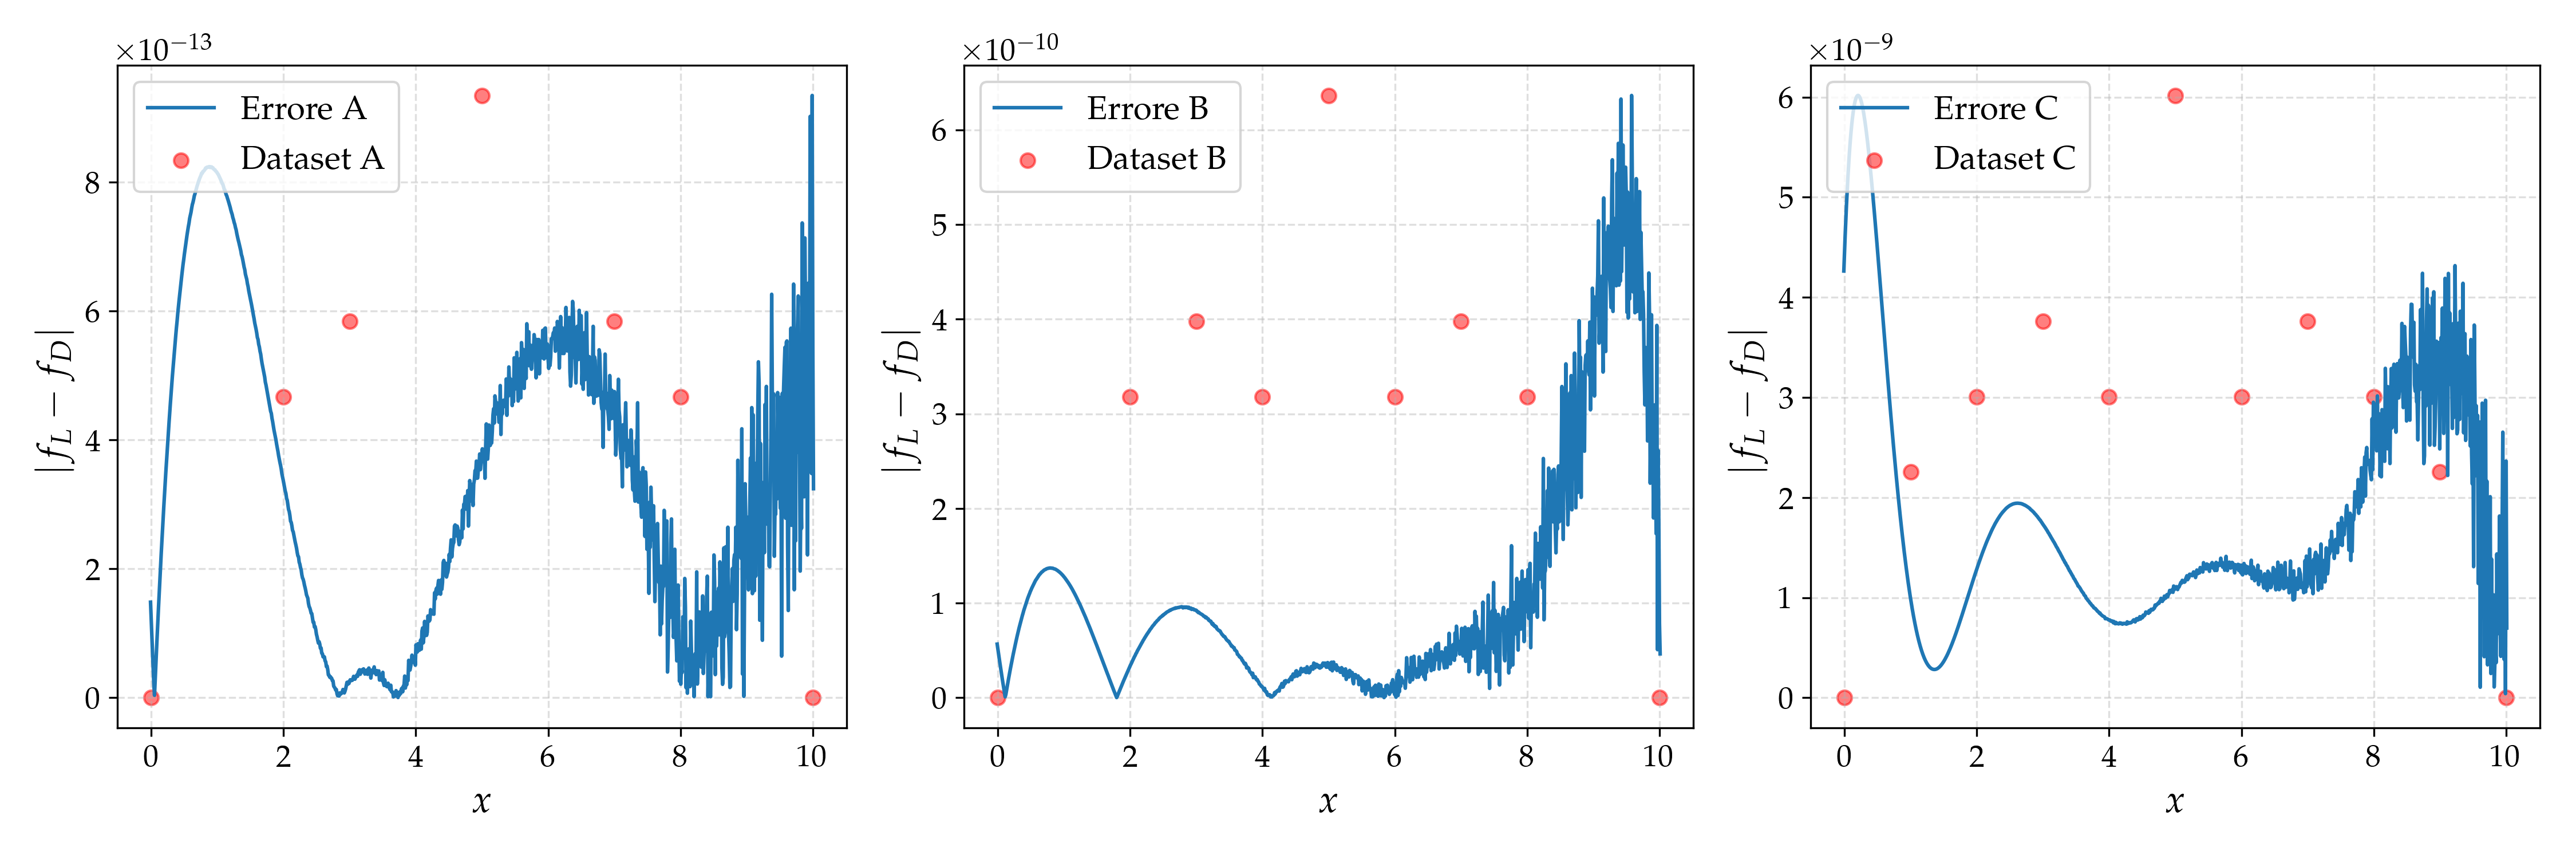
\includegraphics[width=\linewidth]{images/8/Err_dir_vs_lag.png}
    \caption{Plot dell'errore assoluto tra i metodi di \textit{Lagrange Interpolation} e \textit{Direct Method}, sui differenti dataset definiti in Fig. \ref{fig: Repr dataset}, che sono rappresentati in sovraimpressione, normalizzati per essere confrontabili con le dimensioni dell'errore.}
    \label{fig: Err dir vs lag}
\end{figure}
\newpage





\section{Esercizio 4.2.1}
\subsection{Problem Statement}
Si consideri la funzione di Runge
\[
\frac{1}{1 + 25x^2}.
\]
nel’intervallo $I=[-1,1]$. Calcolare la funzione interpolante utilizzando $N = 10, 20, 30, 40, 50$ nodi definiti sia come nodi equispaziati sia come nodi di Chebyshev. Utilizzare l’interpolatore basato sui polinomi di Lagrange e la \textit{monomial basis} (\textit{direct method} tramite matrice di Vandermonde).

\subsection{Premessa Teorica}
Nel contesto dell'interpolazione polinomiale di punti risulta interessante valutare le conseguenze date dal \textit{\textbf{Teorema di Stone-Weierstrass}}, che ci portano ad affermare che:
\begin{quote}
    ``Per un'interpolazione polinomiale, aumentando il numero di punti, cioè il grado del polinomio, è possibile aumentare anche l'accuratezza.''
\end{quote}

\noindent Ciò però non ci dice quale sia il metodo migliore nè stabilisce che tutti gli algoritmi siano equivalenti; l'esempio della funzione di Runge ci permette di mostrare l'efficacia di un modello diverso da quello utilizzato fin'ora negli esempi che abbiamo presentato. Si può mostrare come la scelta del sampling non uniforme con i \textit{nodi di Chebyschev} rappresenta un esempio di metodo che permette di risolvere il fenomeno di Runge.
 
\subsection{Metodi Numerici e Algoritmi}

\medskip
\noindent La funzione di Runge è definita come:
\[
f(x) = \frac{1}{1 + 25x^2}.
\]
ed è possibile mostrare come, per questo esempio, l'accuratezza della funzione interpolata, in $I$, diminuisca rispetto al modello al crescere del numero di punti che campioniamo, se scegliamo un campionamento uniforme. 

Un esempio in Fig. \ref{fig: Lag unif} dove il numero di nodi (uniformi) varia nell'intervallo $[10, 60]$ ed è possibile osservare come solo nell'intorno del massimo si migliori l'accuratezza; verso gli estremi accade il contrario, in maniera che la differenza con $f(x)$ sia assolutamente non trascurabile. 
Se definiamo i \textit{nodi di Chebyschev} come:
\[
x_j = -\cos \left( \frac{j\pi}{n-1} \right) \quad j = 0, 1 \dots n-1
\]
cioe come punti equidistanti su una circonferenza unitaria, ma proiettati sul suo diametro. Si può dimostrare che questo diventa un migliore sampling per l'intervallo $I$, come mostra il confronto con la Fig. \ref{fig: Lag Cheby}. I nodi di Chebyshev riducono l’errore massimo e, per funzioni regolari, favoriscono la convergenza dell’interpolante.

 \begin{figure}[H]
     \centering
     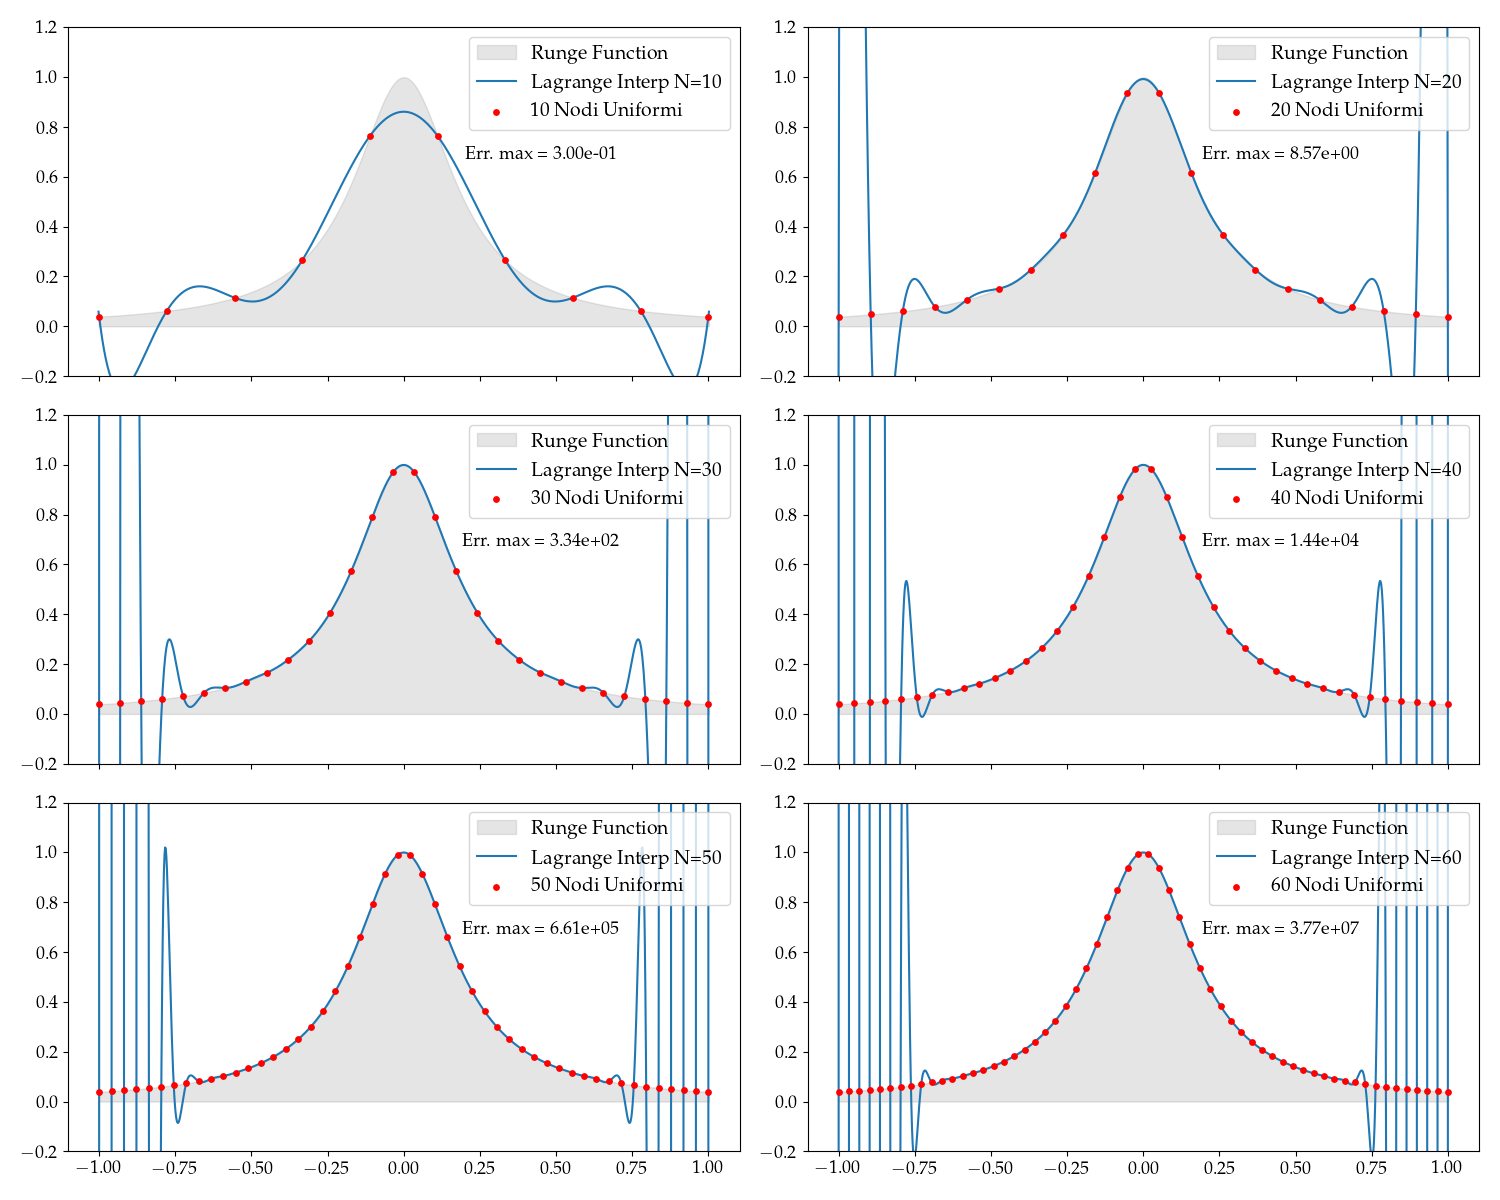
\includegraphics[width=\linewidth]{images/9/lagr_unif.png}
     \caption{\textit{Lagrange interpolation} di $f(x)$ in $[-1,1]$, nodi uniformi.}
     \label{fig: Lag unif}
 \end{figure}

\begin{figure}[H]
    \centering
    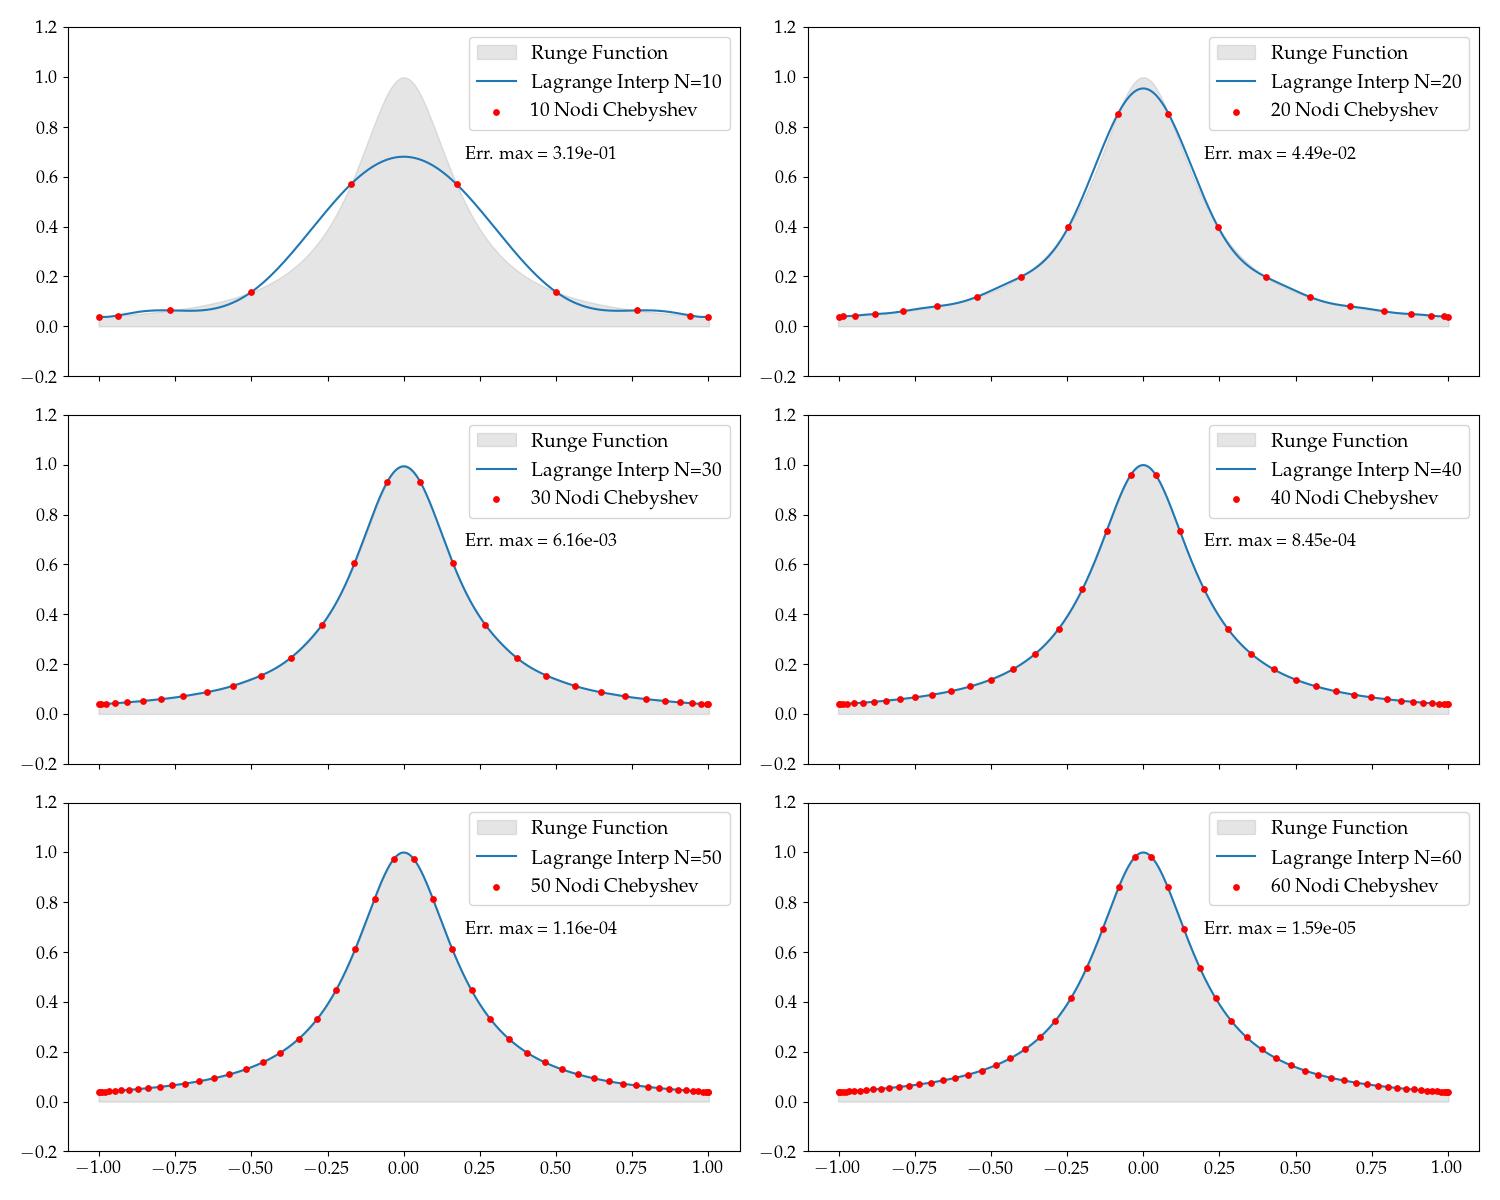
\includegraphics[width=\linewidth]{images/9/lagr_cheby.png}
    \caption{\textit{Lagrange interpolation} di $f(x)$ in $[-1,1]$, nodi di Chebyschev.}
    \label{fig: Lag Cheby}
\end{figure}
     
\subsection{Risultati e Discussione}
Le figure che abbiamo mostrato sottolineano la praticità e correttezza dell'utilizzo del sampling dei \textit{nodi di Chebyschev} per un algoritmo di intepolazione più accurato. \noindent Nelle stesse figure a cui avevamo fatto riferimento, indicato in sovraimpressione, abbiamo anche l'errore massimo nei nodi, nel confronto con $f(x)$: si osserva numericamente, nei plot di Fig. \ref{fig: Lag unif err} e Fig. \ref{fig: Lag cheby err} una crescita molto rapida (quasi esponenziale) che si ha all'aumentare del numero di nodi uniformi interpolanti, mentre un fenomeno opposto con i nodi di Chebyschev. 

\begin{figure}[H]
    \centering
    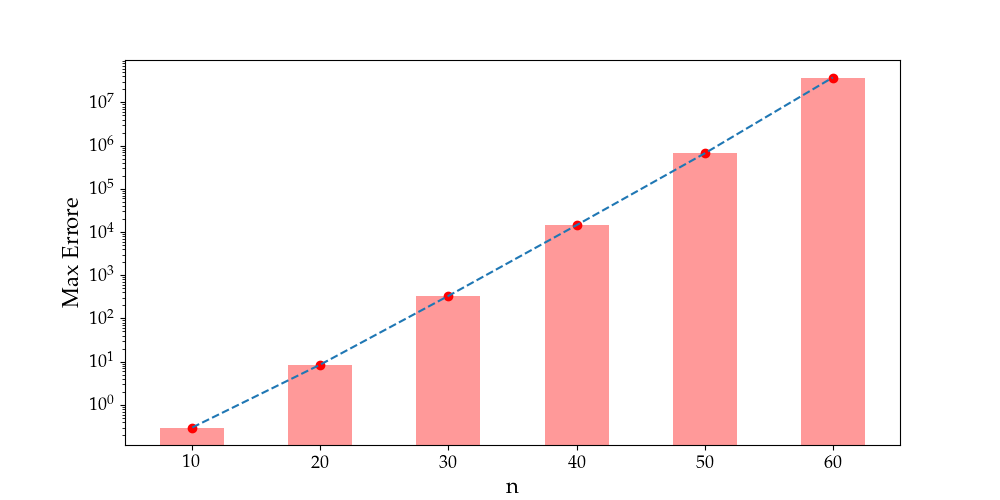
\includegraphics[width=0.8\linewidth]{images/9/unif_err.png}
    \caption{Errore massimo della funzione interpolata al variare del numero di nodi uniformi: è possibile osservare come l'\textit{Err Max} aumenti in maniera esponenziale, usando questo metodo.}
    \label{fig: Lag unif err}
\end{figure}

\begin{figure}[H]
    \centering
    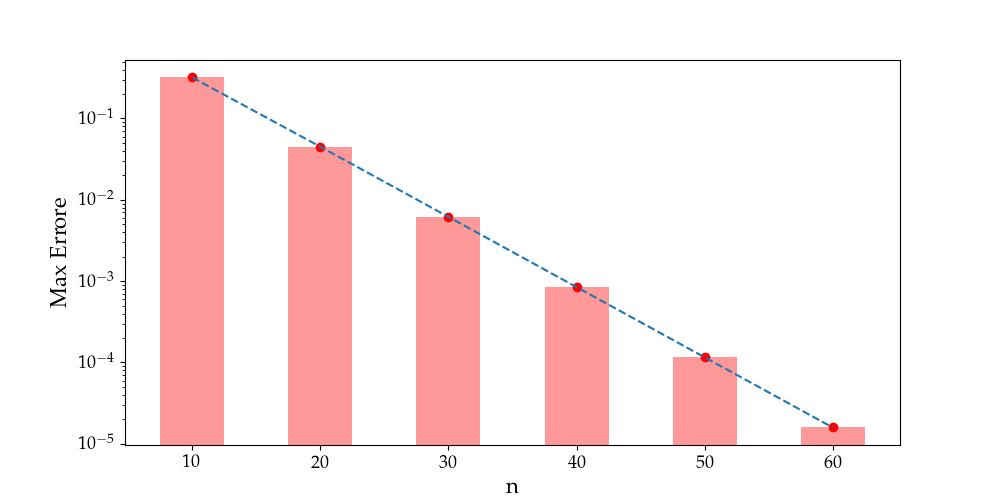
\includegraphics[width=0.8\linewidth]{images/9/cheby_err.png}
    \caption{Errore massimo della funzione interpolata al variare del numero di nodi di Chebyschev: vi è una decrescita esponenziale.}
    \label{fig: Lag cheby err}
\end{figure}

\noindent Infine ci interessa sottolineare che questo fenomeno non è proprio del metodo di interpolazione che abbiamo scelto, che per gli esempi precedenti era stato la \textit{Lagrange Interpolation}, difatti possiamo mostrare come anche per un metodo alternativo, scegliamo il \textit{Direct method}, è possibile mostrare lo stesso fenomeno di Runge.

\begin{figure}[H]
    \centering
    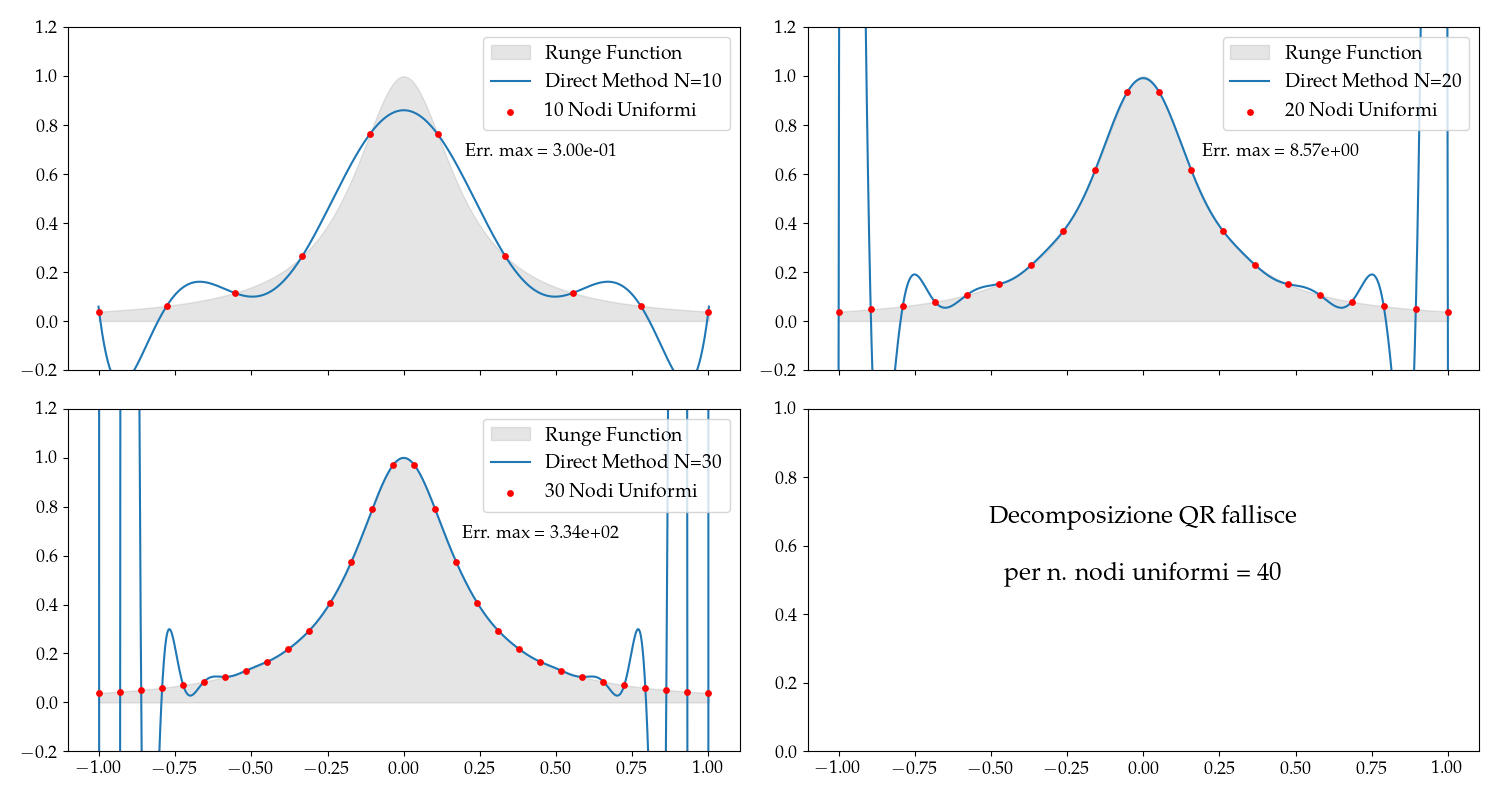
\includegraphics[width=0.8\linewidth]{images/9/direct_unif.png}
    \caption{\textit{Direct method} su $f(x)$ in $[-1,1]$, nodi uniformi. Sono note dal Cap. \ref{Cap: Direct Mth} le problematiche di questo metodo di interpolazione, che risultano più evidenti all'aumentare del numero di nodi: il risultato diventa numericamente instabile per $n \gtrsim 40$ a causa del mal condizionamento della matrice di Vandermonde.”}
    \label{fig: Direct unif}
\end{figure}

\begin{figure}[H]
    \centering
    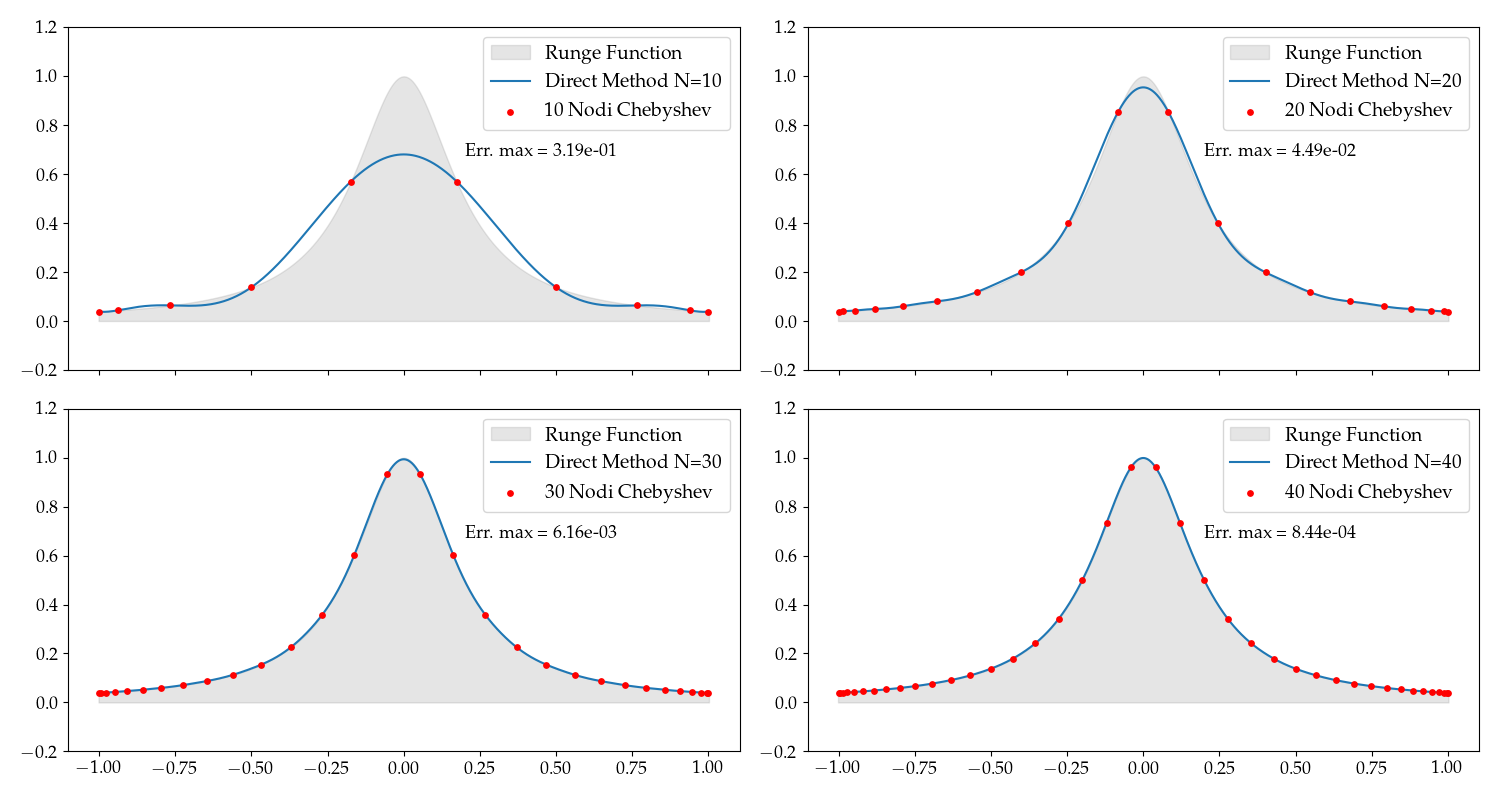
\includegraphics[width=0.8\linewidth]{images/9/direct_cheby.png}
    \caption{\textit{Direct method} su $f(x)$ in $[-1,1]$, nodi Chebyschev. Il metodo fallisce per $n \gtrsim 50$.}
    \label{fig: Direct cheby}
\end{figure}

\newpage








\section{Esercizio 4.4.1}
\subsection{Problem Statement}
Scrivi una classe che, dato l'insieme discreto di coordinate $x_i$, calcoli e memorizzi la matrice $W_{ij}$. 
Aggiungi i metodi \texttt{dft} e \texttt{idft}, entrambi i quali accettano un array della stessa lunghezza di $\{x_i\}$ 
e restituiscono la DFT diretta o inversa (internamente i due metodi applicano 
la matrice $W$ o la sua aggiunta $W^\dagger$). Partendo dai seguenti parametri:
\begin{itemize}
    \item $L = 2\pi$
    \item $N = 128$
    \item $\alpha = 0.5$
    \item $u(x, 0) = \sin(x) + 0.5 \sin(3x)$
\end{itemize}

\noindent Risolvi l'equazione del calore 1D implementando questi passaggi:
\begin{enumerate}
    \item Applica la DFT diretta a $u(x, 0)$ e calcola $\tilde{u}(k, 0)$
    \item Calcola $\tilde{u}(k, t)$
    \item Applica la DFT inversa a $\tilde{u}(k, t)$ per trovare $u(x, t)$
\end{enumerate}

\noindent Ripeti questa operazione per 20 valori di $t \in [0, 2]$ e poi plottali insieme.

\subsection{Premessa Teorica}
\subsubsection{Interpolazione Trigonometrica}
nei capitoli precedenti ci siamo occupati di interpolazioni lineari, cioè in cui vale che:
\[
P(x) = \sum a_k \phi_k(x)
\]
in particolare scegliendo $\phi_k(x) = x^k$, cioè definendo un'interpolazione polinomiale. Un'alternativa a questo approccio è data da un'interpolazione trigonometrica, cioè in cui $\phi_k(x) = e^{ikx} = \omega^k, \quad \omega = e^{ix}$. Questa diventa un'estensione complessa della base dei monomi, permettendo di estendere anche il teorema di unicità, che affermava:

\bigskip
\noindent Dato l'insieme di $N$ punti $x_k = 2\pi k/N$, con $k = 0, 1 \dots N - 1$, per ogni insieme di punti di supporto $(x_k, f_k)$, con $f_k$ complesso, esiste un unico polinomio

\[
P(x) = \sum_{k=0}^{N-1} a_k e^{ikx}
\]

\noindent che soddisfa $P(x_k) = f_k$ per ogni $k$. Definendo $\omega_k = e^{ix_k} = e^{2\pi i k/N}$, i coefficienti possono essere calcolati esplicitamente utilizzando

\[
a_k = \frac{1}{N} \sum_{j=0}^{N-1} f_j \omega_j^{-k} = \frac{1}{N} \sum_{j=0}^{N-1} e^{-2\pi ijk/N} f_j
\]

\noindent In genere, i coefficienti $a_k$ sono chiamati la trasformata di Fourier di $f$ e vengono indicati con $\tilde{f}_k$.
Definendo $\Delta x = L/N$, cioè il passo di sampling regolare su un intervallo $[0, L]$, definiamo la \textit{Trasformata di Fourier diretta} (DFT):
\[
\tilde{f}(p) = \Delta x \sum_{i=0}^{N-1} f(x_i) e^{ipx_i}
\]
dove p è il momento, cioè la coordinata nello spazio di Fourier. La trasformata inversa (IDFT) diventa quindi:
\[
f(x_i) = \frac{1}{L} \sum_{j=0}^{N-1} e^{-ip_j x_i} \tilde{f}(p_j)
\]

\subsubsection{Equazione del calore 1D}
In particolare la FT ci viene in aiuto come metodo standard per risolvere alcuni tipi di equazioni differenziali: nello spazio dei momenti la derivata rispetto alle coordinate diventa un semplice prodotto, semplificando molto il calcolo, in particolare consideriamo l'equazione del calore 1D su un dominio $x \in [0, L]$ con condizioni al contorno periodiche:

\begin{equation} \label{eq: Heat eq}
\frac{\partial u}{\partial t} = \alpha \frac{\partial^2 u}{\partial x^2}, \quad u(x, 0) = f(x)
\end{equation}

\begin{itemize}
    \item $u(x, t)$ è la temperatura alla posizione $x$ e al tempo $t$,
    \item $\alpha$ è la diffusività termica,
    \item $f(x)$ è la distribuzione iniziale di temperatura.
\end{itemize}

se valutiamo la trasformata del lato sx e dx:
\begin{itemize}
    \item $\mathcal{F} \left[ \frac{\partial u}{\partial t} \right] = \frac{\partial \tilde{u}}{\partial t}$
    \item $\mathcal{F} \left[ \frac{\partial^2 u}{\partial x^2} \right] = -p^2 \tilde{u}$
\end{itemize}

quindi l'equazione si riduce ad una ODE:
\[
\frac{\partial \tilde{u}}{\partial t} = -\alpha p^2 \tilde{u}
\]

la cui soluzione analitica è:
\[
\tilde{u}(p,t) = \tilde{u}(p,0) e^{-\alpha p^2t}
\]
La condizione sul valore iniziale è nota, risulta sufficiente calcolare la trasformata del valore iniziale; abbiamo quindi la soluzione nello spazio dei momenti, basta una IFT per tornare nello spazio delle coordinate e risolvere Eq. \ref{eq: Heat eq}
\[
\tilde{u}(p,t) \longrightarrow u(x,t)
\]

\subsection{Metodi Numerici e Algoritmi}
Per implementare la risoluzione del problema proposto risulta naturale passare ad una espressione matriciale della definizione della DFT e IDFT:
\[
\tilde{f}_k = \Delta x \sum_{i} W_{ki} f_i \quad \quad W_{ki} = e^{i p_k x_i}
\]
Questo offre la possibilità di usare gli algoritmi già sviluppati per la risoluzione dei sistemi lineari, in più permette un semplice passaggio da DFT a IDFT, che necessiterebbe di invertire $W$, ma che diventa il banale calcolo di $W^\dagger$:
$$W^\dagger W = N I \implies W^{-1} = \frac{1}{N} W^\dagger \implies W^\dagger = N W^{-1}$$
quindi:
\[
\tilde{f}_k = \Delta x \sum_{i} W_{ki} f_i \quad \quad f_i = \frac{1}{L} \sum_{k} W^\dagger_{ik} \tilde{f}_k 
\]

\medskip
\noindent Questa la classe che abbiamo implementato nel nostro codice \textit{.py}:
\begin{elegantcode}
class DFT:
    def __init__(self, x_desc):
        N = len(x_desc)
        L = (x_desc[-1] - x_desc[0])
        
        if N % 2 == 0: 
            p_pos = np.arange(N//2+1)   # positive values bcs of Niquist (even)
            p_neg = np.arange(1, N - (N//2)) * (-1)
        else: 
            p_pos = np.arange(N//2)     # positive values bcs of Niquist (odd)
            p_neg = np.arange(1, N - (N//2)) * (-1)

        p = 2 * np.pi / L * np.concatenate((p_pos, p_neg))
        W = np.exp(1j * np.outer(p, x_desc))

        self.W = W
        self.p = p
        self.N = N
        self.L = L
        self.dx = L / N
    
    def dft(self, y_desc):
        if type(y_desc)==int or len(y_desc) != self.N:
            raise ValueError('len(y_desc) must be equal to len(x_desc)!')
        y_dft = self.dx * self.W @ y_desc
        return y_dft

    def idft(self, y_desc):
        if type(y_desc)==int or len(y_desc) != self.N:
            raise ValueError('len(y_desc) must be equal to len(x_desc)!')
        y_idft = self.L**(-1) * self.W.conj().T @ y_desc
        return y_idft
    
\end{elegantcode}

\subsection{Risultati e Discussione}
L'esercizio permette un'efficace rappresentazione grafica tramite la libreria \textit{matplotlib}, in particolare con l'uso di mappe di colore e curve di livello, che esprimono il variare della $u(x,t)$. Sono mostrate due rappresentazioni differenti del fenomeno: in Fig. \ref{fig: Heat 2d} è dato un plot in cui segnamo diverse curve di livello, corrispondenti ai 20 valori temporali per cui valutiamo la funzione, ogni curva ha assegnato un colore, proprio di un valore temporale. In Fig. \ref{fig: Heat 3d} la rappresentazione è 3d, dove lungo l'asse x e y troviamo $x$ e $t$, mentre l'asse z riporta il valore di $u(x,t)$, anche il colore riporta l'informazione sul valore di $u$.

\bigskip
\noindent Una animazione interessante può essere visualizzata nella mia repo al link: \\
\url{https://github.com/mvolpato-unimib/Lab_comp/tree/d679cbb9a8c50a2e1b8f371e7fc05a3aa251d053/ex10/plots}\\
Il plot "\textit{ani\_col.gif}" è un'animazione di $u_t(x)$, con il plot che si evolve in funzione del tempo. La colorazione dei punti è data dal valore della funzione in x, così che sia accentuato il variare della stessa in $t \in [0, 1]s$. Per le animazioni visibili nella cartella, è stato modificato il parametro $\alpha=0.4$, per ragioni di interesse grafico.


\begin{figure}[H]
    \centering
    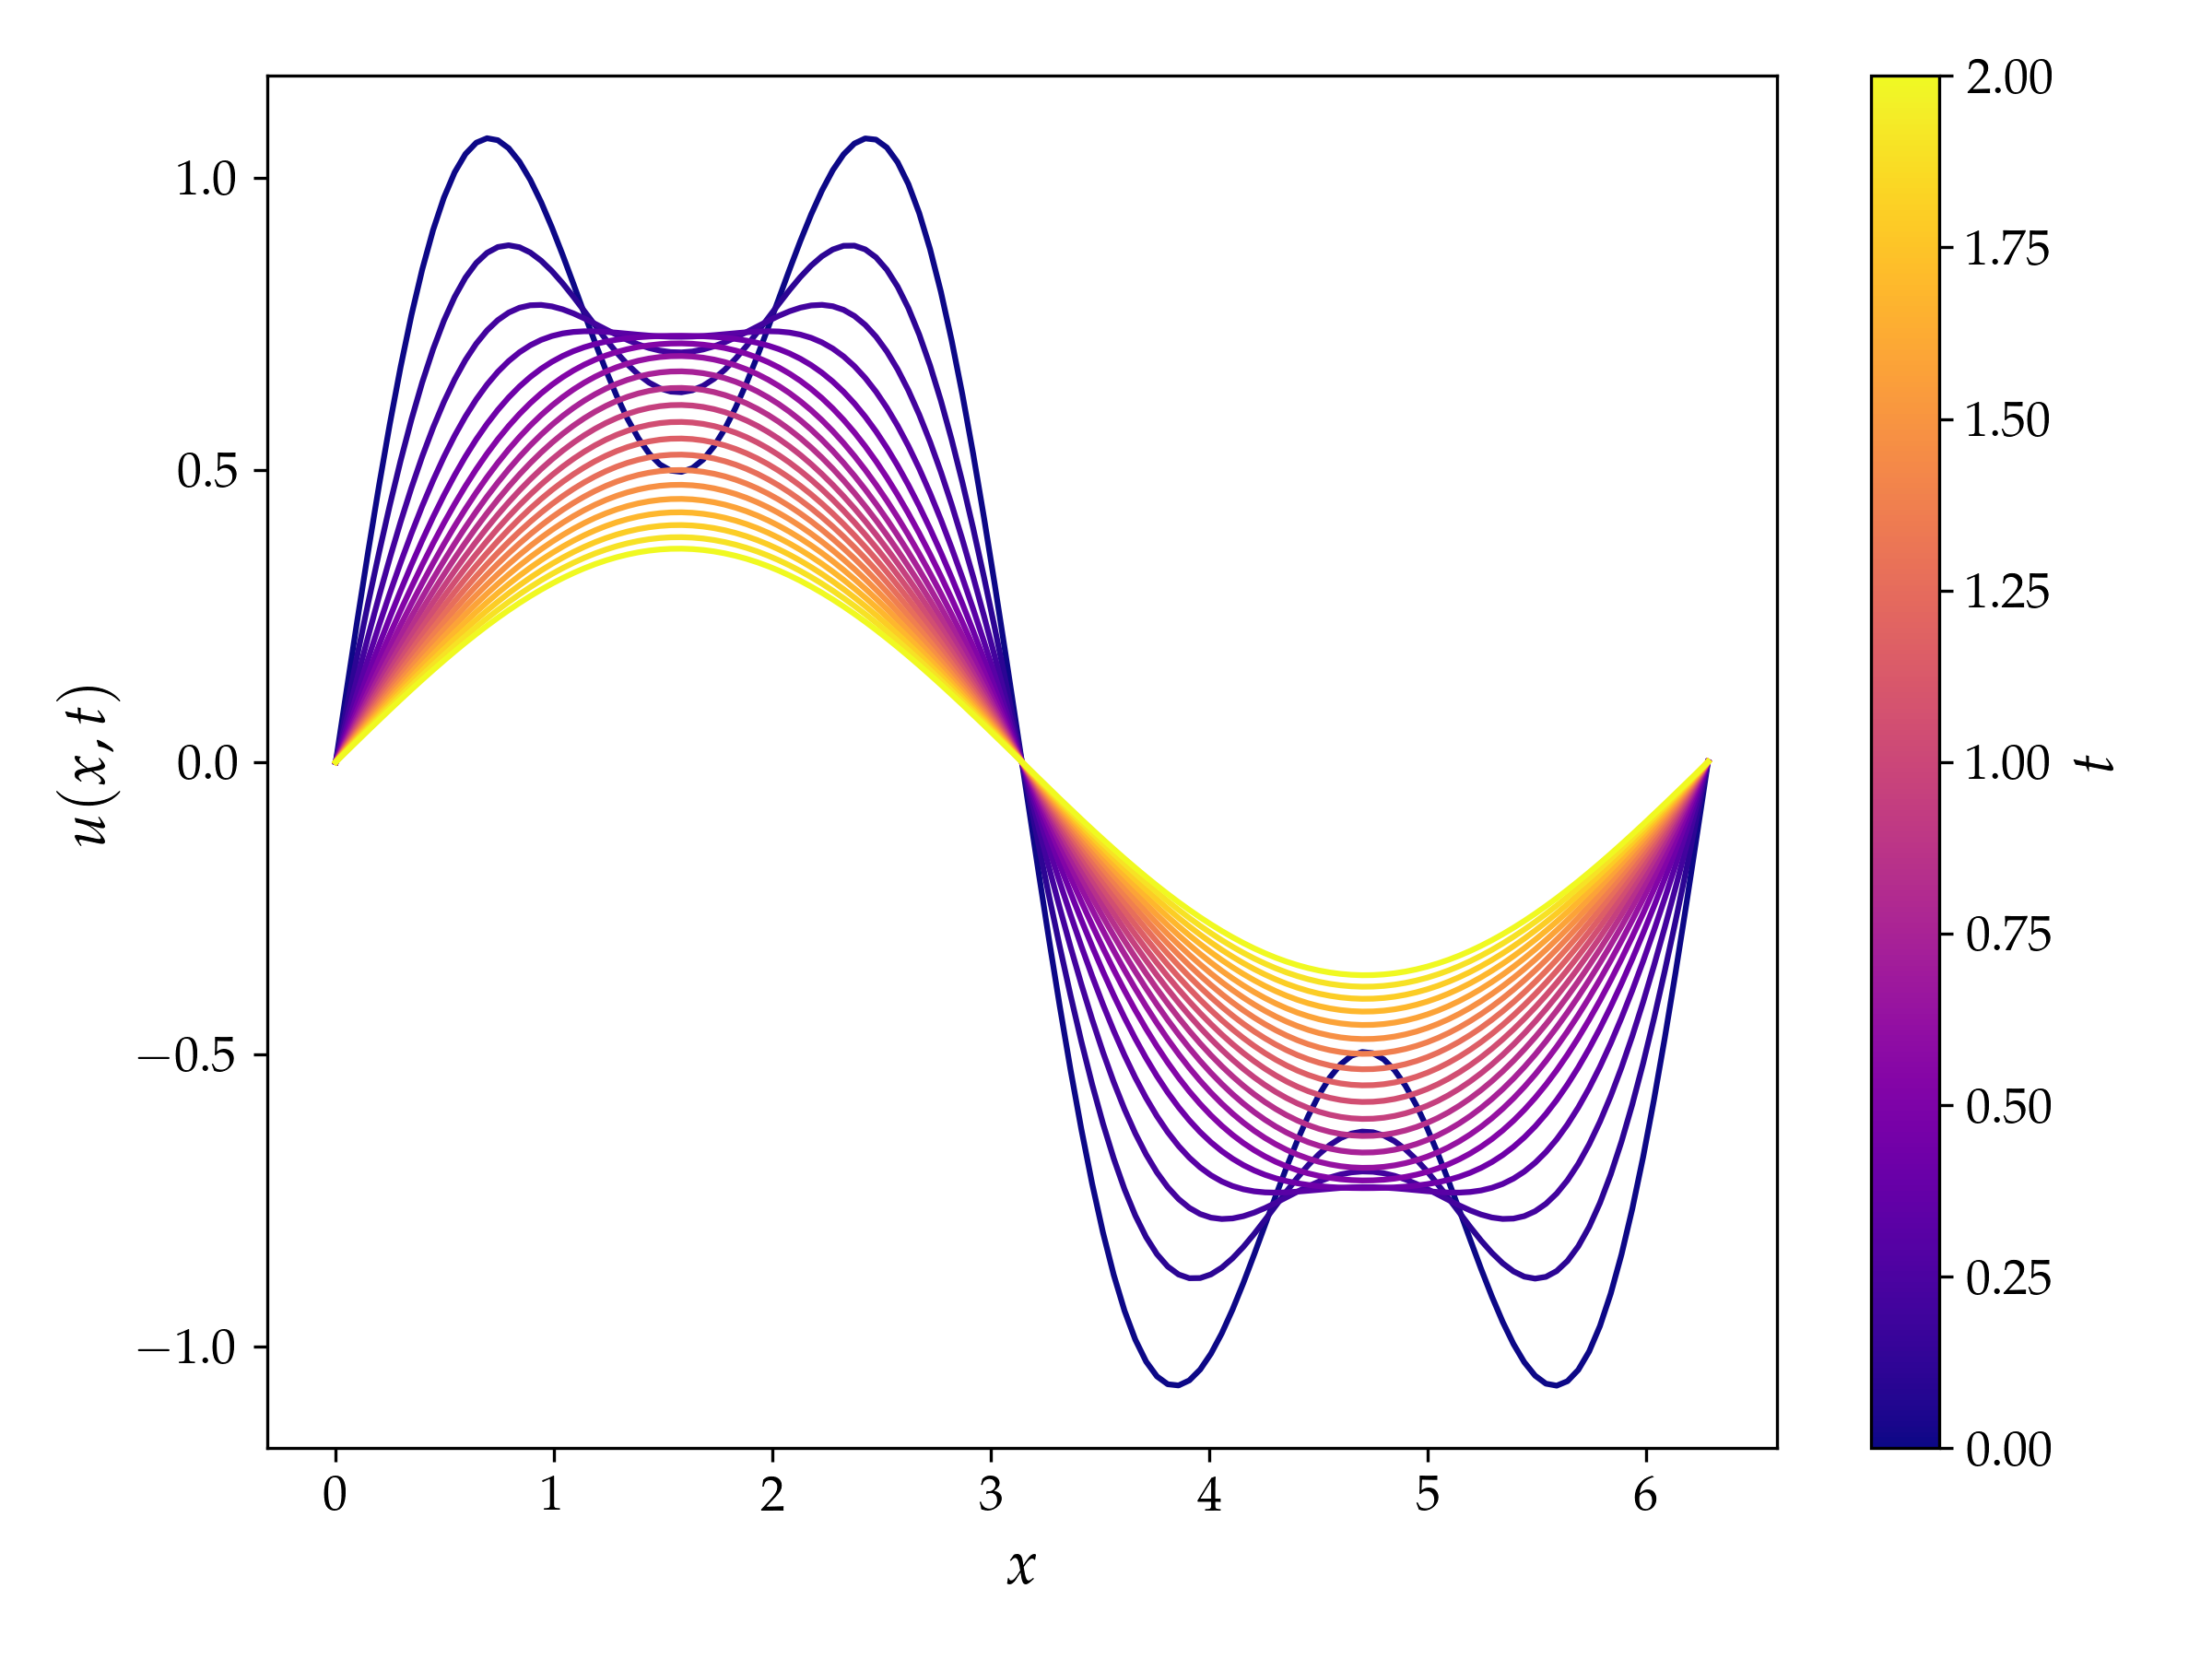
\includegraphics[width=0.8\linewidth]{images/10/heat_sol.png}
    \caption{Variazione del calore in funzione della posizione (asse x) e del tempo (curva di livello con colore assegnato e riportato in legenda).}
    \label{fig: Heat 2d}
\end{figure}

\begin{figure}[H]
    \centering
    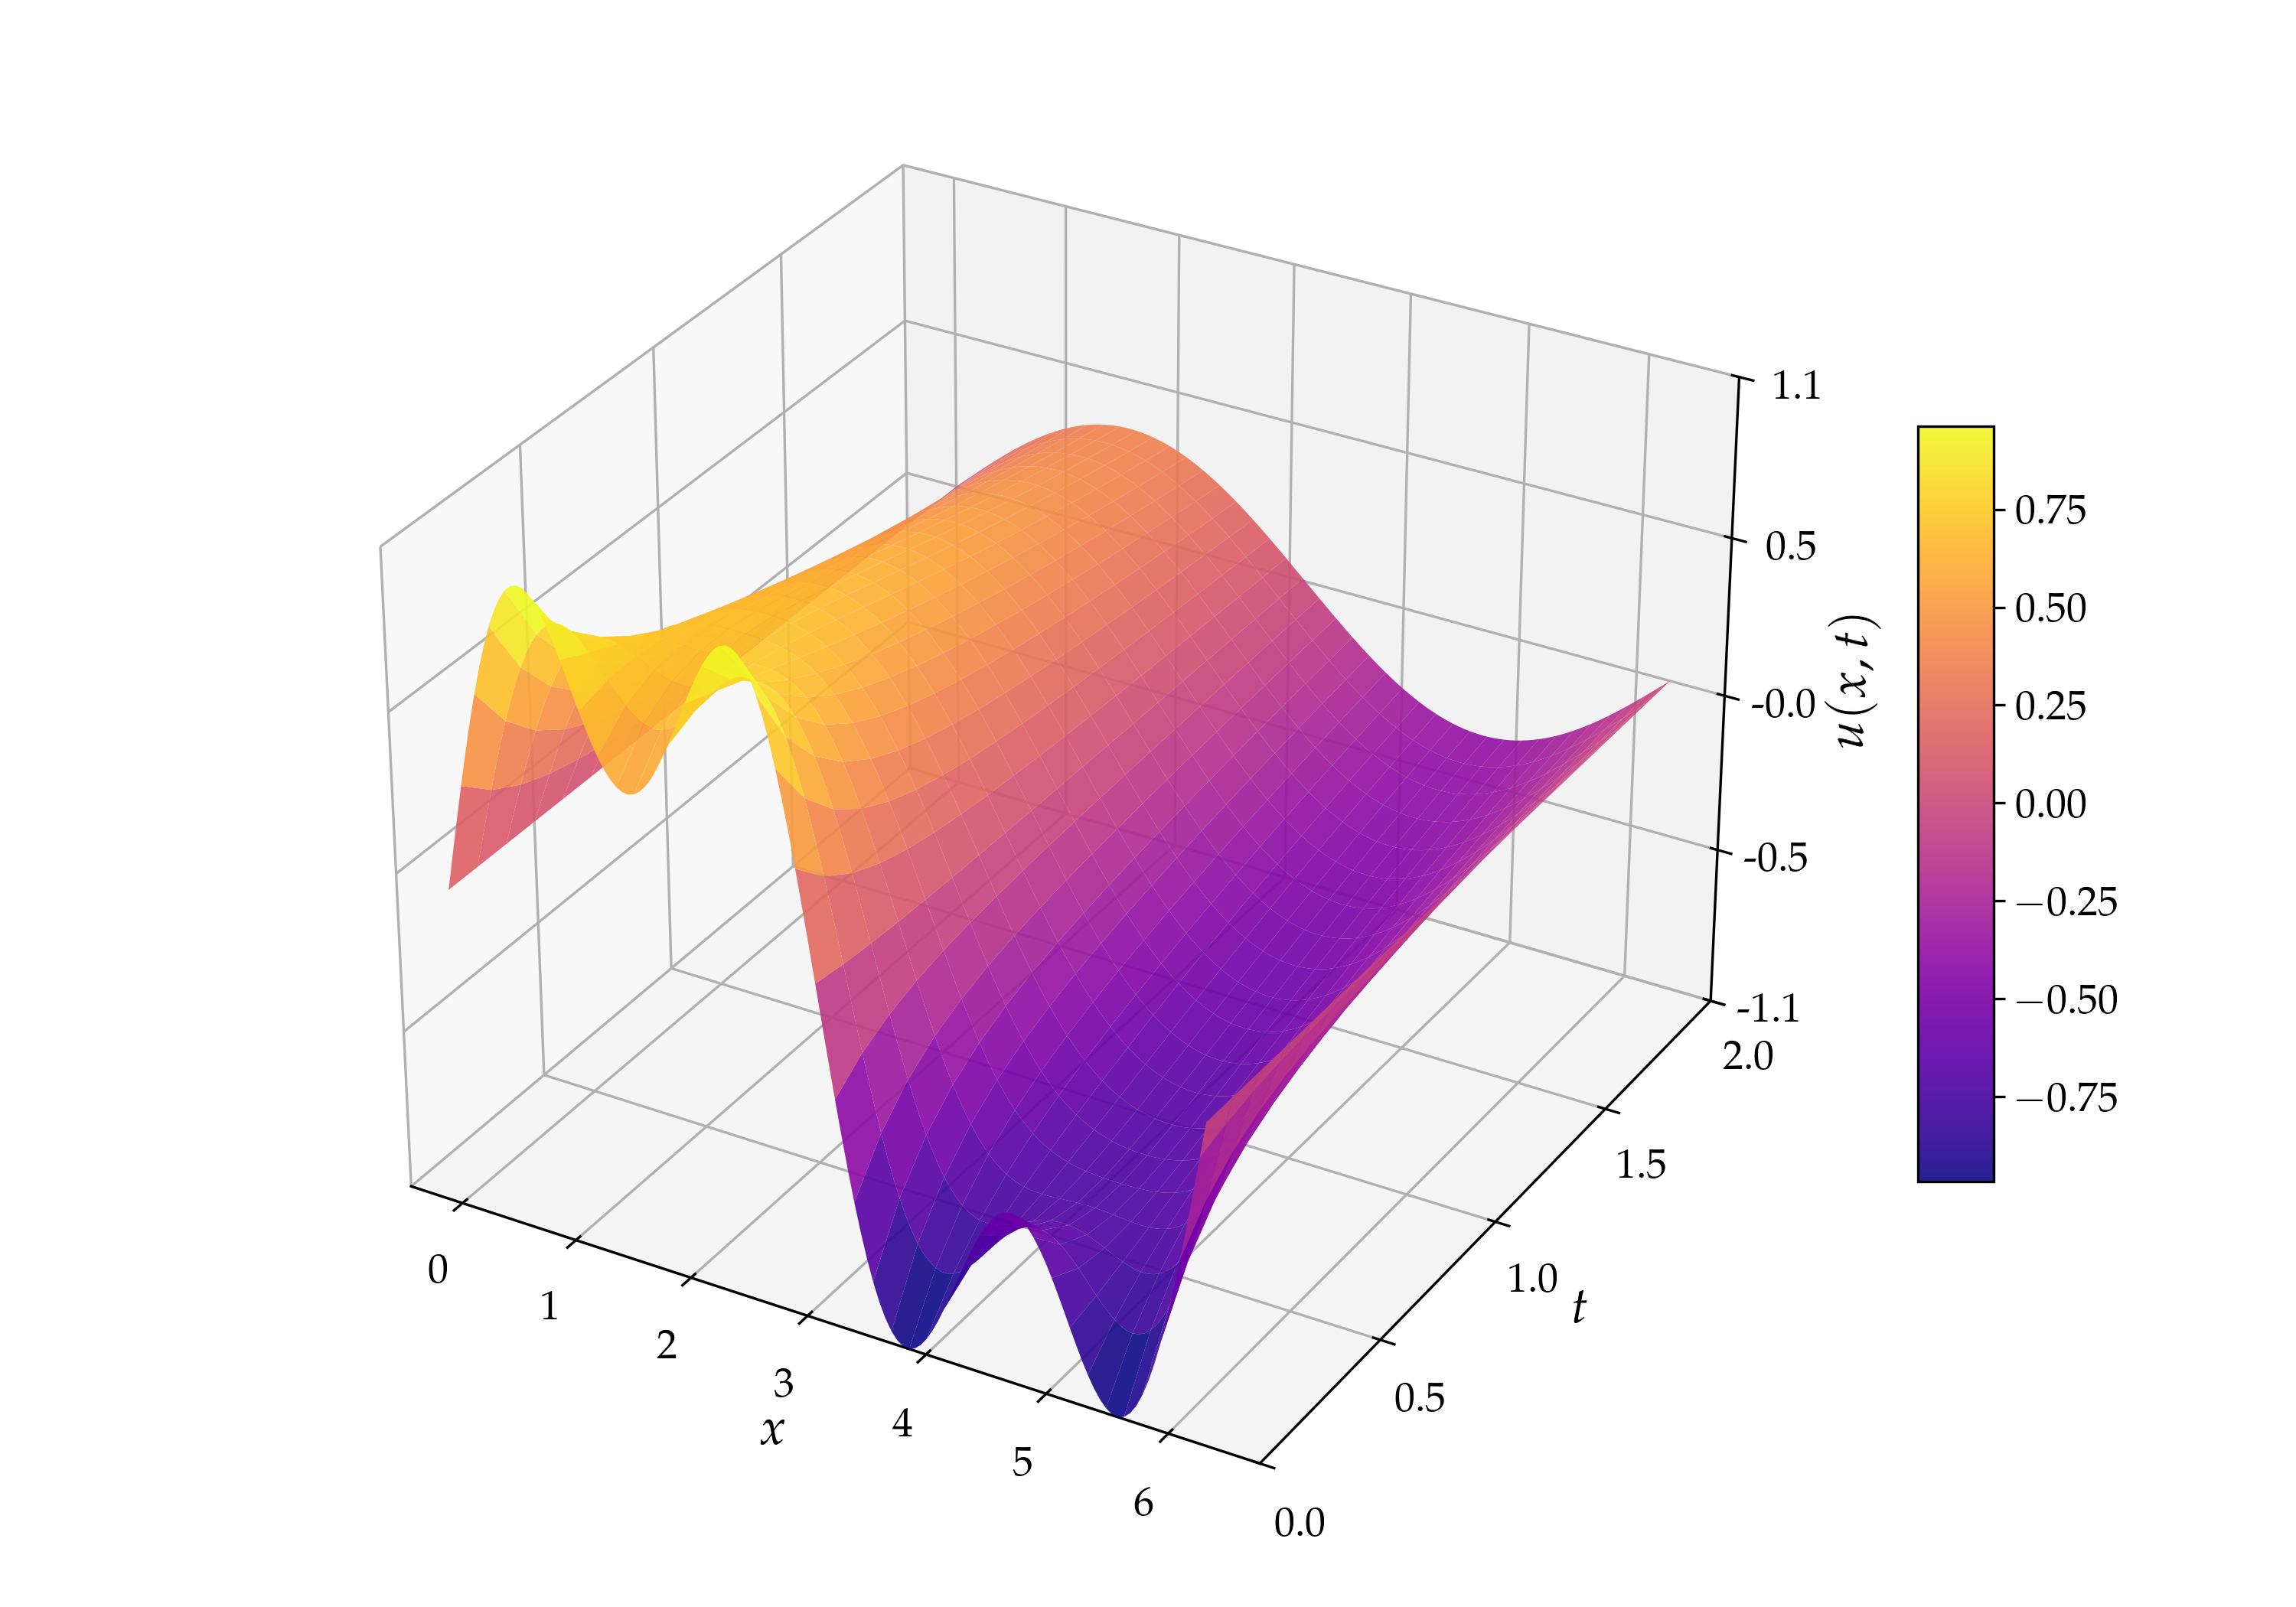
\includegraphics[width=0.8\linewidth]{images/10/heat_sol_3d.png}
    \caption{Variazione del calore in funzione della posizione e tempo con heatmap 3D. Il colore rappresenta il valore della funzione, come riportato in legenda}
    \label{fig: Heat 3d}
\end{figure}

\newpage







\section{Esercizio 4.5.1}
\label{Cap: fitting}
\subsection{Problem Statement}
Scrivi una funzione che accetti $\{x_i\}$, $\{y_i\}$, $C_{ij}$ e $\{f_a\}$ e restituisca il valore del $\chi^2$ insieme ai parametri del fit e ai loro errori.
Quindi testa la funzione sui dati forniti utilizzando
\[
    \frac{F}{(E - M)^2 + \left(\frac{\Gamma}{2}\right)^2}
\]

\noindent Nota che la forma funzionale non è lineare nei parametri ma una semplice trasformazione può renderla tale! Pertanto dovresti procedere come segue:

\begin{enumerate}
    \item trasforma i dati in modo che la funzione di fit sia lineare nella base monomiale. Produci un grafico dei dati trasformati.
    \item esegui il fit sui dati trasformati e calcola i parametri $F, M, \Gamma$ e il $\chi^2$. È un buon fit?
    \item produci un grafico con i dati trasformati e la funzione di fit.
    \item produci il grafico finale con le seguenti caratteristiche:
    \begin{itemize}
        \item i dati originali (con gli errori)
        \item una linea che rappresenta il valore centrale della funzione di fit
        \item \textit{opzionale}: una banda che rappresenta l'errore della funzione di fit ottenuta propagando gli errori dei parametri del fit.
    \end{itemize}
\end{enumerate}

\subsection{Premessa Teorica}
Se il problema dell'interpolazione è in soprattutto un problema di tipo matematico, in questo contesto vogliamo dare la risoluzione di uno fisico. Partendo da un set di due coordinate, di una forma funzionale che ne descrive la relazione, e degli errori che sono associati al valore sperimentale della funzione, è possibile definire un metodo che esegua un'operazione di grande interesse fisico-sperimentale: in particolare si tratta di verificare il grado di compatibilità dell'osservazione con il modello (test $\chi^2$) e calcolare il valore dei parametri liberi che vengono determinati dall'assunzione del modello come valido.

\medskip
Il set di dati è $\boldsymbol{x}_i$ e $\boldsymbol{y}_i$ rappresenta il valore sperimentale della funzione $f(\boldsymbol{x}_i, \boldsymbol{\alpha}_a)$, dove $\boldsymbol{\alpha}_a$ è il vettore dei parametri liberi, quelli che desideriamo stimare con il fit. Se il numero di punti che usiamo per fittare è $N$ e il numero di parametri $N_A$, allora $i = 0, 1, \dots, N-1$  e $a = 0, 1, \dots ,N_A-1$; 
\begin{itemize}
    \item $N = N_A \implies$ Tutti i parametri possono essere fissati esattamente, Fit $\equiv$ Interpolazione.
    \item $N \gg N_A \implies$ È possibile trovare la soluzione migliore minimizzando la norma $\chi^2$:
    $$\chi^2 = [y_i - f(x_i, \boldsymbol{\alpha})] W_{ij} [y_j - f(x_j, \boldsymbol{\alpha})]$$
    la matrice $W$ è quadrata e definita positiva; nel caso di fit con errori sui dati, che sono raccolti nella matrice di covarianza ($C_{ij}$), è utile scegliere $W_{ij}=C_{ij}^{-1}$, poiché questa scelta permette di interpretare il test del $\chi^2$ e il suo \textit{p-val} come significativi della bontà del fit.
\end{itemize}

\subsubsection{La \textit{Normal equation}}
Se è possibile ottenere una funzione lineare nei parametri, è possibile interpretare la risoluzione del problema di fitting come un sistema di equazioni lineari, già discusso nella Parte \ref{Cap: Matrici e Sistemi Lineari}.\\
Definendo $F_i$ come:
\[
F_i = F(x_i) = \sum_{a=0}^{N_a-1} \alpha_a f_a(x_i) =
\sum_{a=0}^{N_a-1} \alpha_a X_{ia}, \quad \quad X_{ia} = f_a(x_i)
\]

\noindent così il residuo nel $\chi^2$ è semplicemente:
\[
    \boldsymbol r =\boldsymbol  y - \boldsymbol  \alpha \, X
\]
\[
\implies \chi^2 = (y^T - \alpha^T X^T) W (y - X\alpha)
\]

$$\xrightarrow{\text{svolgendo}}\chi^2 = y^T Wy - y^T W X\alpha - \alpha^T X^T Wy + \alpha^T X^T W X\alpha$$
$y^T W X \alpha = \alpha^T X^T W^T y$ e assumiamo $W=W^T$, cioè simmetrica: si può riscrivere la relazione precedente come

$$\chi^2 = y^T Wy - 2\alpha^T X^T Wy + \alpha^T X^T W X\alpha$$

\bigskip
\noindent Il nostro algoritmo si basa sulla minimizzazione della metrica $\chi^2$, cioè sul valutare $\frac{\partial \chi^2}{\partial \alpha_a} = 0$. Svolgendo le derivate abbiamo il risultato finale:

$$-2X^T Wy + 2X^T WX\alpha = 0 \quad \longrightarrow{} \quad X^T WX \alpha = X^T Wy$$

Cioè risolvendo per $\alpha$, ipotizzando $M = X^T W X$ invertibile:

$$\alpha = M^{-1} X^T Wy$$

Si può verificare che la matrice di covarianza per i parametri fittati sia:
\[
    C_{ab} = M_{ab}^{-1} \implies \sigma_{\alpha_a} = \sqrt{C_{aa}} 
\]

\subsection{Metodi Numerici e Algoritmi}
\subsubsection{Implementazione della \textit{Decomposizione di Cholesky}}
Notando che $M$ è simmetrica e definita positiva, scegliamo di implementare una risoluzione che faccia uso dell'algoritmo di Cholesky (Cap. \ref{Cap: Cholesky}). Recuperando l'equazione appena trovata possiamo riscrivere in maniera da rendere esplicito il sistema lineare $A \boldsymbol{x} = LL^T\boldsymbol{x}= \boldsymbol{b}$:

\[
    M \boldsymbol \alpha = L L^T \boldsymbol \alpha = X^T W \boldsymbol y = \boldsymbol b
\]

\[
    L \boldsymbol x = \boldsymbol b \,, \quad \to \quad L^T \boldsymbol \alpha = \boldsymbol x
\]

\bigskip
\noindent Nell'appendice \hyperref[App: funzione fit]{App.1} segue una breve digressione sull'implementazione che ho deciso di fare per una funzione specifica per il fit, utile e utilizzata per questo esercizio, ma che ho scelto di usare e generalizzato appositamente anche per diversi utilizzi più avanti nel corso del laboratorio: la funzione fa uso proprio dei metodi descritti in questo paragrafo. 

\subsubsection{Fitting della \textit{Breit-Wigner}}
La funzione che ci è richiesto di fittare non è lineare nel parametro $E$, ma lo può diventare se consideriamo una sua riscrittura, quindi:

\[
  \sigma_{BW}(E) = \frac{F}{(E - M)^2 + \left(\frac{\Gamma}{2}\right)^2} \quad \to \quad
  f(E) = 1 / \sigma_{BW}(E) = aE^2 + bE + c 
\]

\noindent dove $a,b,c$ diventano i nuovi parametri del fit lineare, da cui sapremo poi ricavare i parametri originali della \textit{BW} come:
\[
F = 1/a \quad \quad
M = -\frac{b}{2a} \quad \quad
\Gamma = \frac{\sqrt{4ac - b^2}}{a}
\]

\bigskip

\noindent Nella Fig. \ref{fig: Lin_vsNLin} si può osservare il confronto tra le due curve, $\sigma_{BW}(E)$ e $f(E)$; interessante la maniera in cui si trasformano anche gli errori sui punti, che derivano nel plot a sx dalla matrice di covarianza originale, mentre nel plot di dx dalla propagazione dell'errore su $f=1/\sigma$.

\begin{figure}[H]
    \centering
    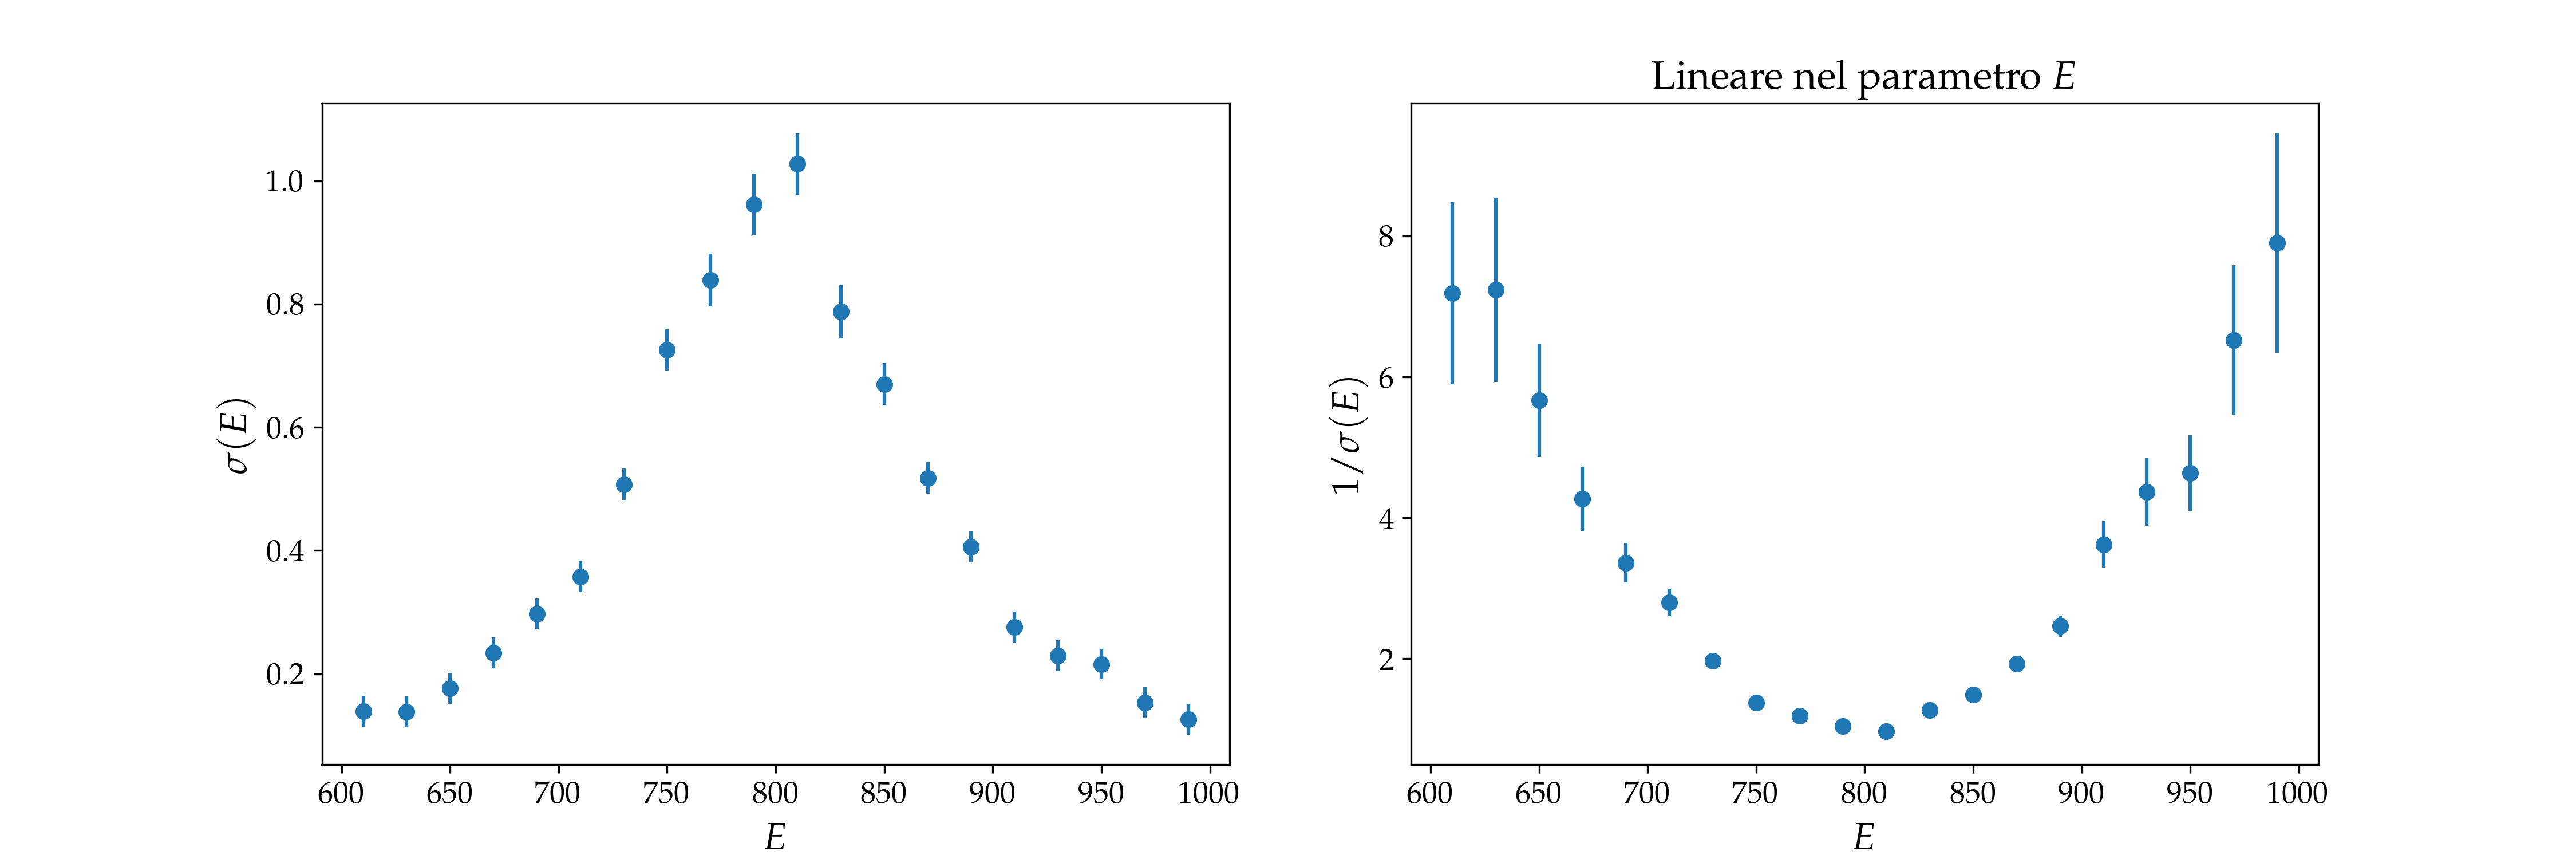
\includegraphics[width=\linewidth]{images/11/confr_lin_nonLin.png}
    \caption{Confronto tra la \textit{BW} e la sua linearizzata.}
    \label{fig: Lin_vsNLin}
\end{figure}


\subsection{Risultati e Discussione}
Esponiamo qui i risultati del fit: partendo dai dati e matrice di covarianza forniti dall'esercizio, procediamo ricavando in primis la matrice di covarianza della funzione linearizzata:
\[
C_{ij}^{(f)} = \frac{\partial f_i}{\partial \sigma_i} C_{ij}^{(\sigma)} \frac{\partial f_j}{\partial \sigma_j} = \frac{1}{\sigma_i^2} C_{ij}^{(\sigma)} \frac{1}{\sigma_j^2}
\]

\noindent Data questa è possibile fittare le $x_i= E_{data}$ con $y_i = \sigma_{data}$, tramite la funzione $f(E)$, già definita precedentemente. Il fit ha queste caratteristiche:
\begin{itemize}
    \item I parametri ottenuti dal fit sono i seguenti:
\begin{center}
    $a = (1.88 \pm 0.10)\times 10^{-4} \text{ MeV}^{-2}$ \\
    \smallskip
    $b = (-3.01 \pm 0.17)\times 10^{-1} \text{ MeV}^{-1}$ \\
    \smallskip
    $c = (1.21 \pm 0.07)\times 10^{2}$
\end{center}
    \item $\chi^2 = 13.5$ ed un corrispondente \textit{p-val($\chi^2$, $\nu$=N-$3$=$17$)} $\approx0.70 \gg 0.05$. I dati hanno una buona aderenza alla funzione $f(E)$ e concludiamo che il fit è buono.

\begin{figure}[H]
    \centering
    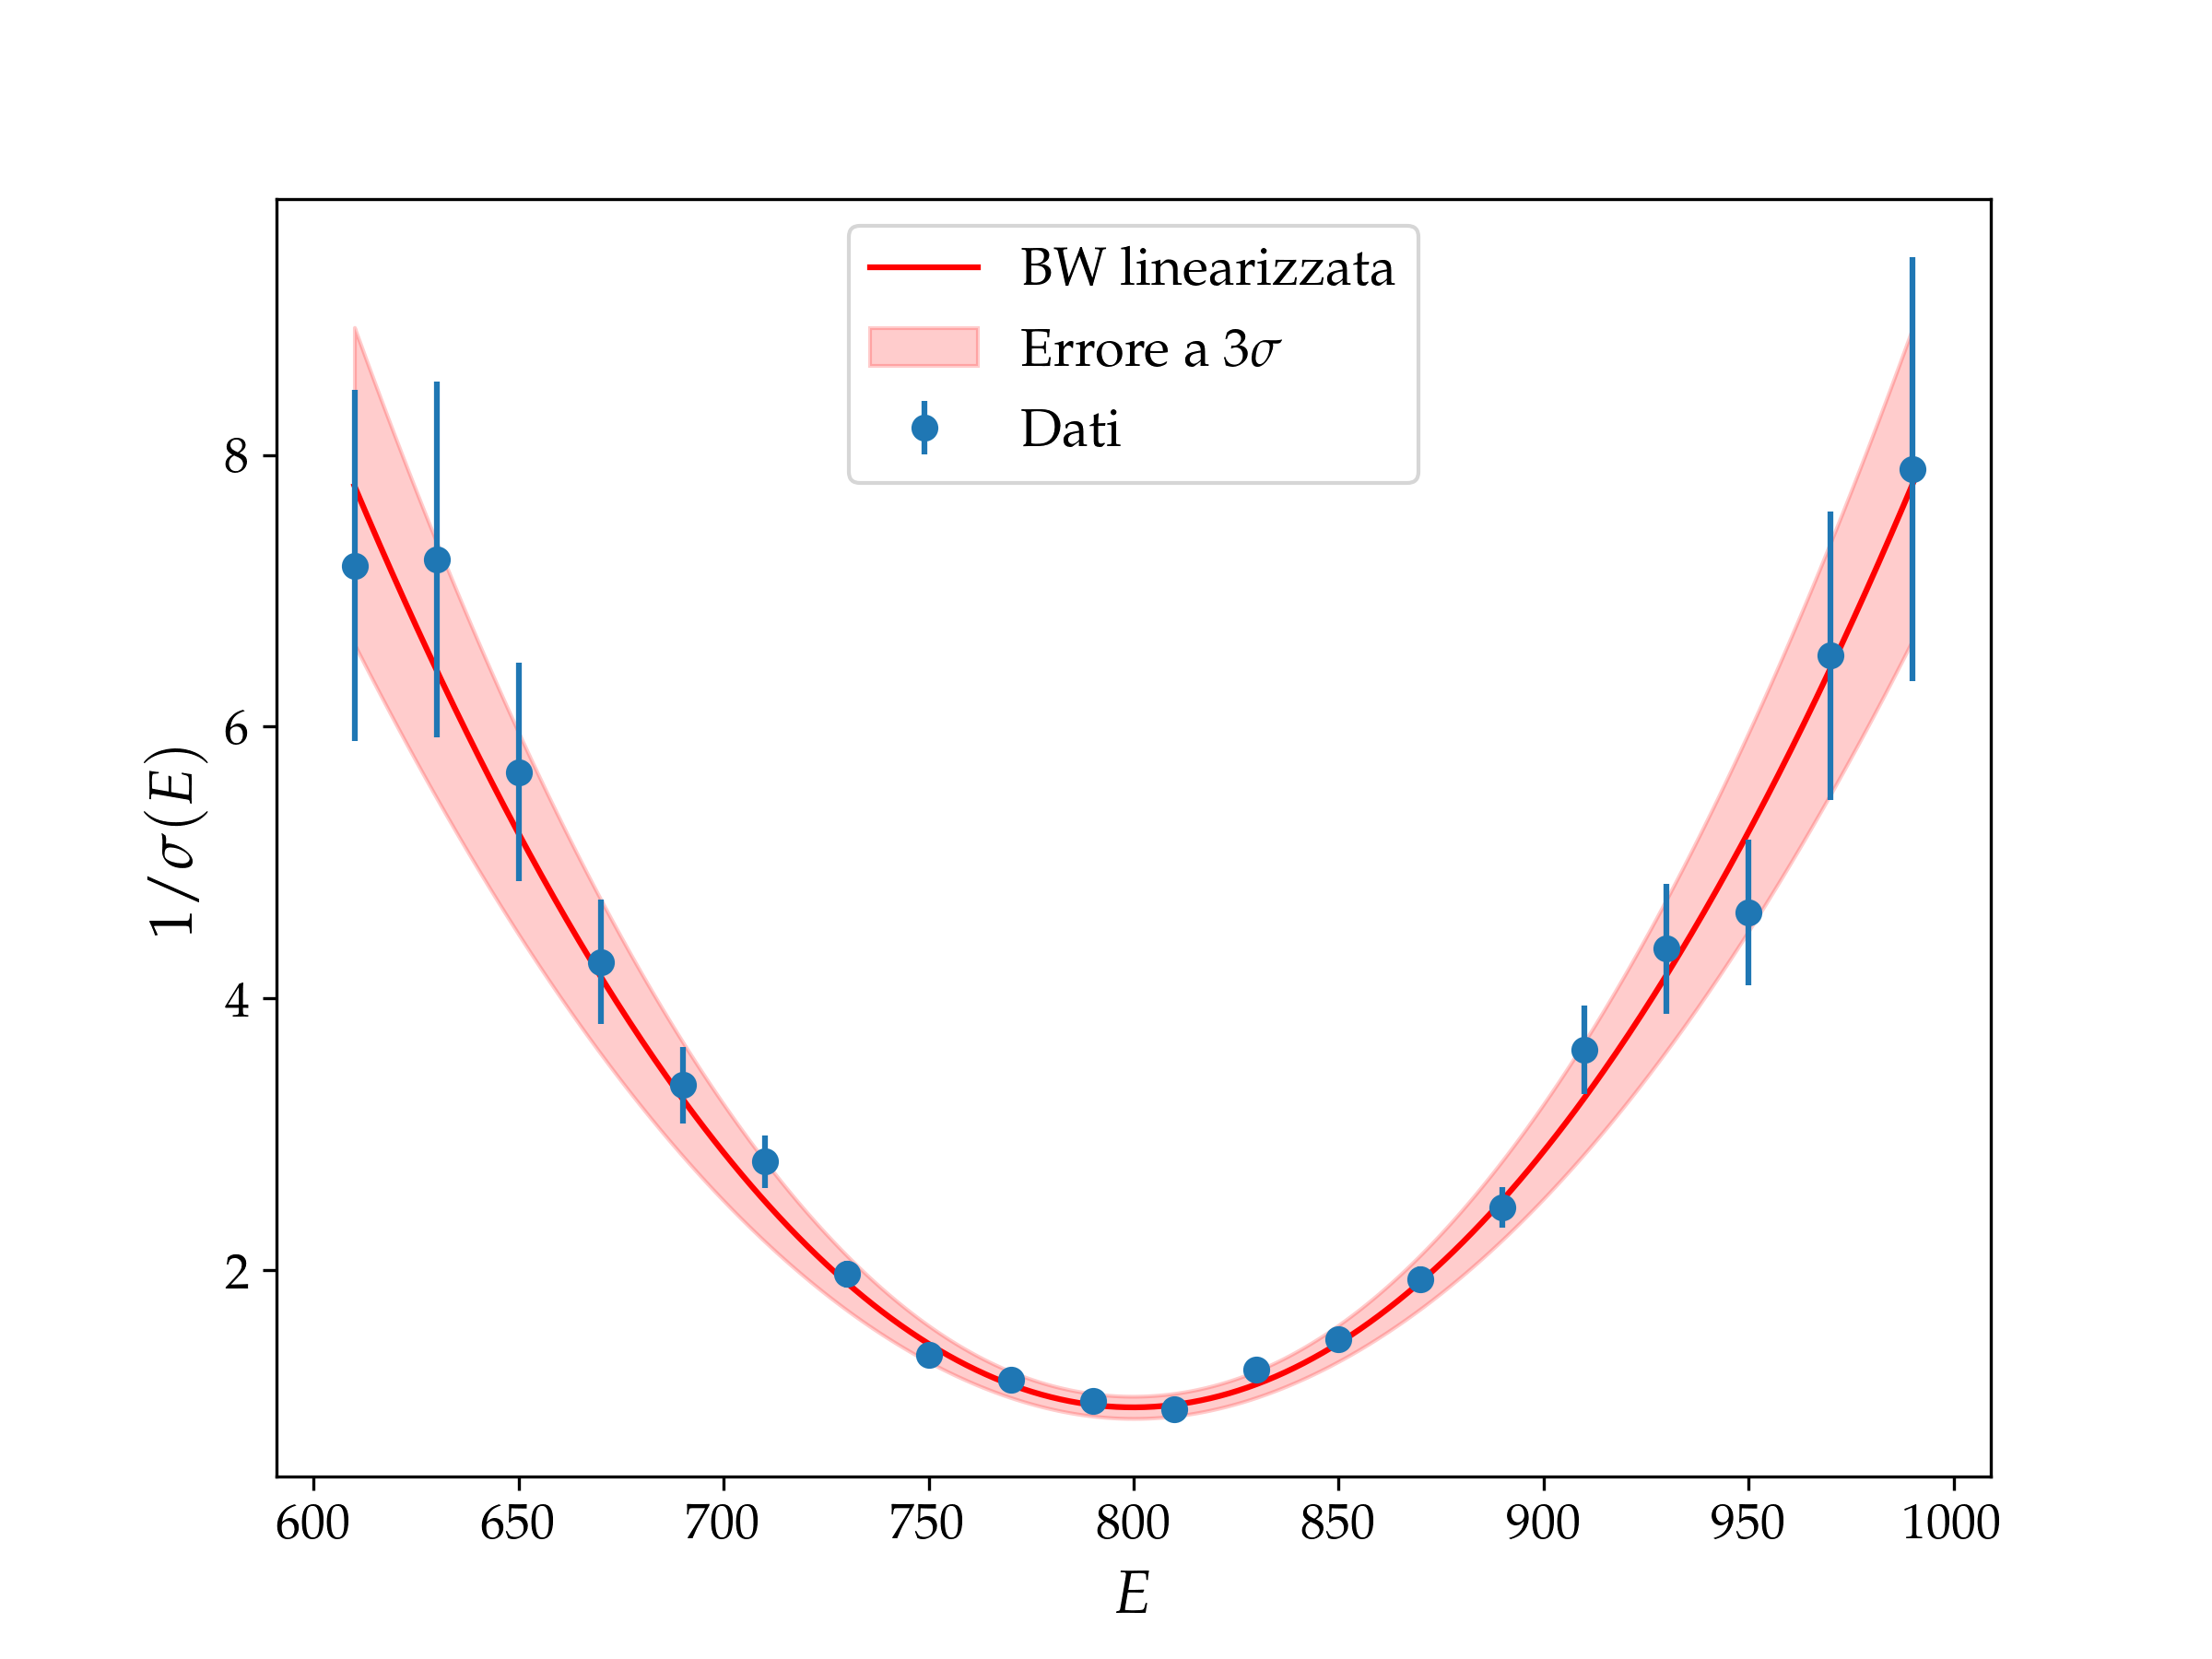
\includegraphics[width=0.68\linewidth]{images/11/Lin_plot.png}
    \caption{Fit della funzione linearizzata, $f(E)$, con errori sui punti e fascia di confidenza a $3\sigma$.}
    \label{fig: Lin_fit}
\end{figure}


    \item Ora possiamo passare ai parametri originali fisici, $F, M, \Gamma$ ed è possibile calcolare i loro errori:
    
\begin{center}
$F = (5.32 \pm 0.29)\times 10^{3} \text{ MeV}^{2}$ \\
\smallskip
$M = (799.9 \pm 1.2) \text{ MeV}$ \\
\smallskip
$\Gamma = (145.1 \pm 5.2) \text{ MeV}$
\end{center}

Possiamo evidenziare la coerenza con quelli che lo statement suggerisce come veri\\($M_{true}=800$ Mev, $\Gamma_{true}=140$ Mev), usati per la generazione del sample.

\begin{figure}[H]
    \centering
    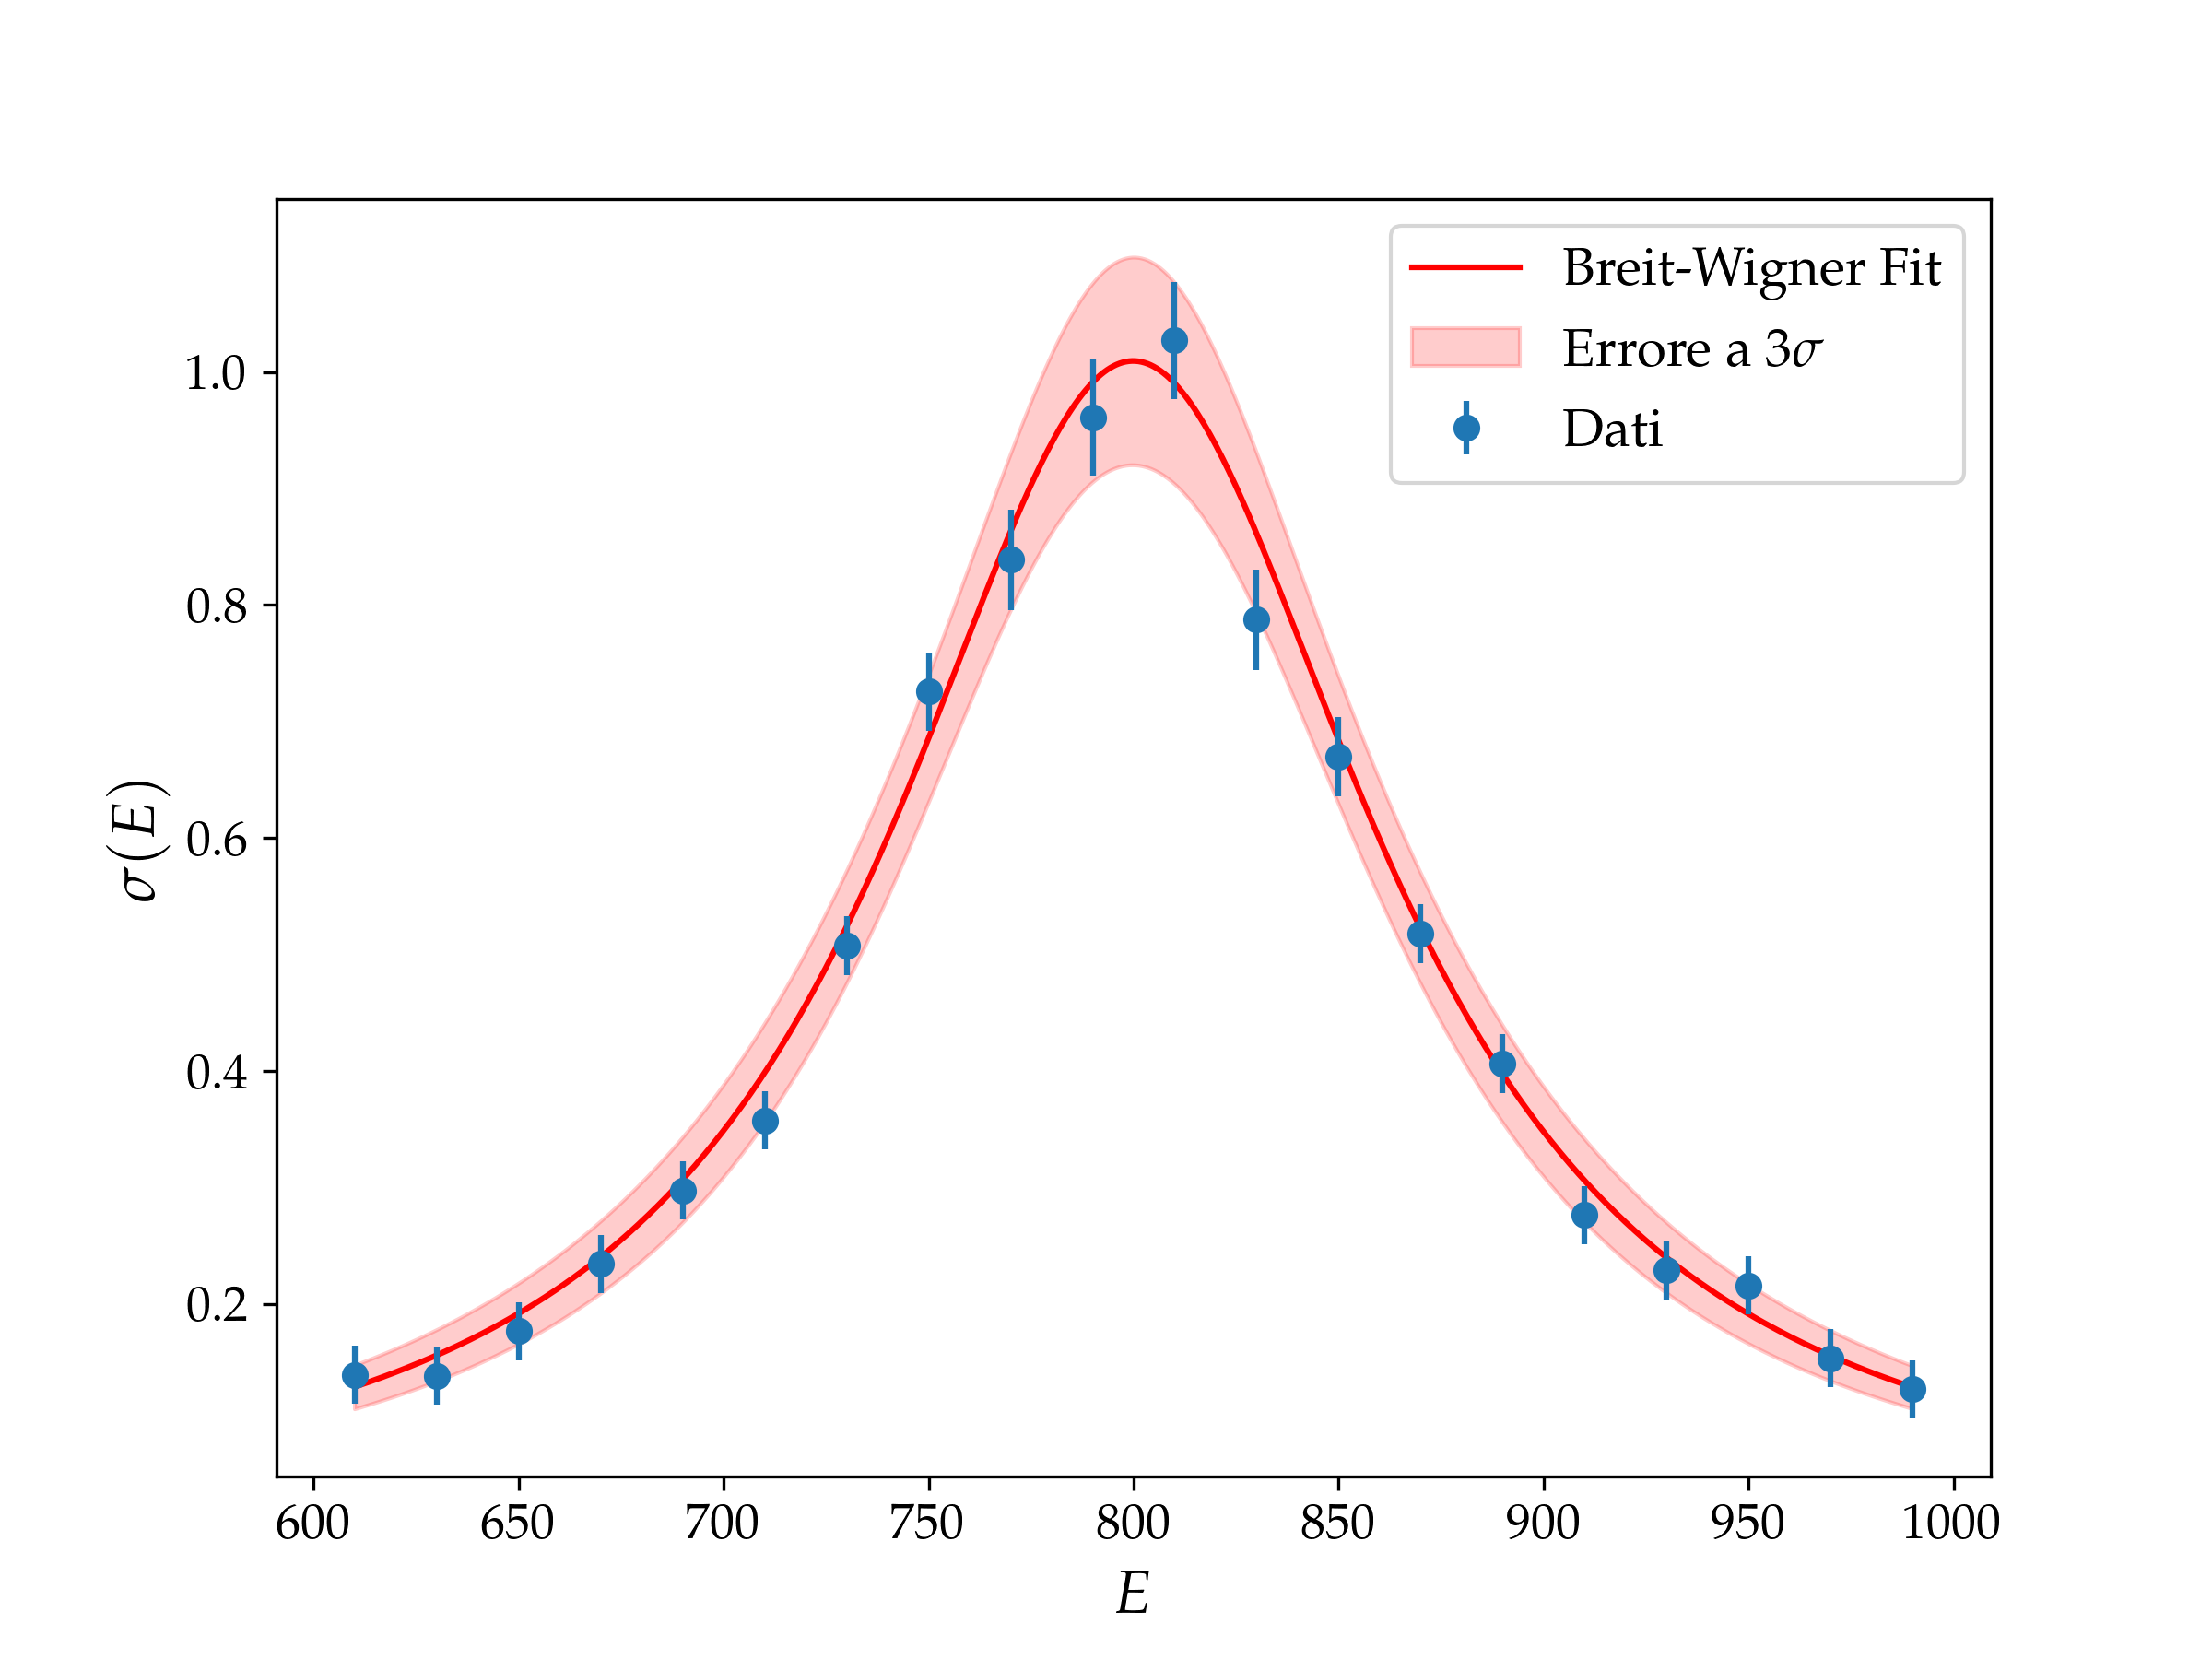
\includegraphics[width=0.68\linewidth]{images/11/Scatt_plot.png}
    \caption{Fit della \textit{Breit-Wigner}, $\sigma_{BW}(E)$, con errori sui punti e fascia di confidenza a $3\sigma$.}
    \label{fig: BW_fit}
\end{figure}
\end{itemize}





% --- PARTE 5: Radici di Funzioni ---
\cleardoublepage 
\addtocontents{toc}{\bigskip\noindent\protect\textbf{\Large Radici di funzioni}\par\smallskip}
\addtocontents{toc}{\protect\setcounter{tocdepth}{-2}} 
\part{\Huge Radici di funzioni}
\addtocontents{toc}{\protect\setcounter{tocdepth}{2}} 


\section{Esercizio 5.1.1}
\subsection{Problem Statement}
\begin{itemize}
    \item Scrivi un programma che implementi l'algoritmo di bisezione e il metodo della Regula Falsi.
    \item Testa i programmi e trova gli zeri della funzione
    
    \[
    f(x) = \frac{1}{2} + x - x^2
    \]
    
    \item Studia la convergenza degli algoritmi, ovvero produci un grafico che dimostri che l'errore diminuisce con il numero di iterazioni. Grafica sia $|f(c_n)|$ che l'errore $|c_n - c|$ in funzione del numero di iterazioni.
\end{itemize}

\subsection{Premessa Teorica}
L'algoritmo di bisezione è un potente, seppur semplice, metodo numerico per trovare gli zeri di una funzione (nell'ipotesi che la funzione sia ben definita nell'intervallo di interesse e che esista almeno uno zero in questo intervallo). La forza del \textit{Bisection method} sta nell'essere un algoritmo \textit{bracketed} (o \textit{bounded}), cioè che dato un certo numero di passaggi fissato da un limite massimo della tolleranza dell'algoritmo, esso troverà una soluzione al problema. Bisogna sottolineare che l'algoritmo converge al valore vero per un numero infinito di passaggi, ma che nella pratica saremo costretti a limitare il suo procedimento con una soglia di tolleranza $\varepsilon$, fissata piccola.


\subsection{Metodi Numerici e Algoritmi} \label{sec. bisec e Regula Falsi}
\subsubsection{Bisezione}
Per implementarlo scegliamo un intervallo di partenza, all'interno del quale sappiamo che sia presente una radice della funzione. È noto che data una funzione continua su un intervallo $I= [a,b]$, il cui il valore agli estremi di $I$ sia discorde in segno, si può affermare che esiste almeno una radice interna ad $I$: l'unica condizione per la bisezione è quindi di avere $f(a)\cdot f(b) < 0$.\\

La ricerca di $c$ t.c. $f(c)=0$ procede dimezzando l'intervallo per ogni iterazione e modificando gli estremi di $I$, cioè:
\[
I = [a,b]\ \longrightarrow\ c = \frac{1}{2}(a+b)
\]

\begin{itemize}
    \item $f(a)\cdot f(c) < 0 \implies b \leftarrow{} c$
    \item $f(a)\cdot f(c) > 0 \implies a \leftarrow{} c$
\end{itemize}
L'algoritmo viene interrotto solo quando si raggiunge una condizione di uscita:
\begin{itemize}
    \item $|f(c)| \le \varepsilon \quad \longrightarrow \quad $ l'algoritmo resituisce $c$
    \item $|b-a| < \varepsilon  \quad \longrightarrow \quad $ questo è il caso in cui non raggiungo la tolleranza ma dividere nuovamente porta a una distanza tra gli estremi confrontabile con $\varepsilon$, quindi ogni punto all'interno del nuovo intervallo è sufficientemente preciso e può essere preso come radice, scegliamo $c=\frac{1}{2}(a+b)$
\end{itemize}

\bigskip
\noindent Dopo $n$ iterazioni l'intervallo è stato dimezzato $n$ volte, quindi 
$$b_n - a_n=\frac{1}{2^n}(b-a)$$
chiaramente l'algoritmo converge per $n\to \infty$ e possiamo valutare l'errore al passo n-esimo come:
\[
    |c_n - c |  \leq \frac{1}{2^n} (b_0 - a_0)
\]
La convergenza è quindi lineare.

\subsubsection{Regula Falsi}
Il secondo algoritmo che analizziamo è quello di \textit{Regula Falsi}, che consiste semplicemente in una ottimizzazione della bisezione con un criterio di \textit{guess} di c più oculato.\\
Dovendo già valutare la funzione nei punti $a,b$, è possibile usare queste informazioni per spingere la ricerca ancora più direttamente verso il valore vero. Possiamo fare una semplice interpolazione, cioè trovare la retta che passa per $(a, f(a))$ e per $(b, f(b))$: quando raggiungiamo una larghezza dell'intervallo sufficientemente piccola, questa approssimazione della funzione con questa secante diventa buona e lo zero dell'interpolante tende a quello della funzione. 
$$
    I(x) = f(a) + \frac{f(b)-f(a)}{b-a} (x-a)
$$
fissando $I(c) = 0$ e risolvendo analiticamente:
\[
    c = \frac{a f(b) - b f(a)}{f(b) - f(a)}
\]

Sarà facile dimostrare numericamente come in molti casi questa scelta acceleri la convergenza, anche se ciò non è garantito in generale.

\subsection{Risultati e Discussione} \label{sec: risultati bisec regula}
Nell'esercizio si richiede di analizzare in particolare il caso della funzione
\[
f(x) = \frac12 + x - x^2
\]
la cui soluzione analitica, nell'intervallo $I=[0,2]$ è
\[
c_{true} = \frac{1 + \sqrt{3}}{2} \approx 1.3660254037844386
\]

\bigskip
\noindent Dopo aver implementato due funzioni che eseguono gli algoritmi descritti precedentemente osserviamo per il caso specifico quali sono i risultati:

\begin{elegantcode}
- BISECTION MTH
     Found f(c) = 0:  c =  1.3660254031419754
     N_iter =  27

- Regula Falsi
     Found f(c) = 0:  c =  1.3660253992204199
     N_iter =  16

diff = 3.921555524755149e-09
\end{elegantcode}

Nella figura sotto rappresentiamo la funzione e il valore di $c \approx 1.37$ trovato dai due algoritmi. La differenza tra i due valori trovati è trascurabile. Si noti \textit{diff} è dell'ordine di $10^{-9}$, cioè inferiore al valore che abbiamo impostato per la tolleranza nell'implementazione ($\varepsilon = 10^{-8}$): i due algoritmi differiscono per meno della nostra precisione, cioè, per le nostre analisi, restituiscono lo stesso valore.

\begin{figure}[H]
    \centering
    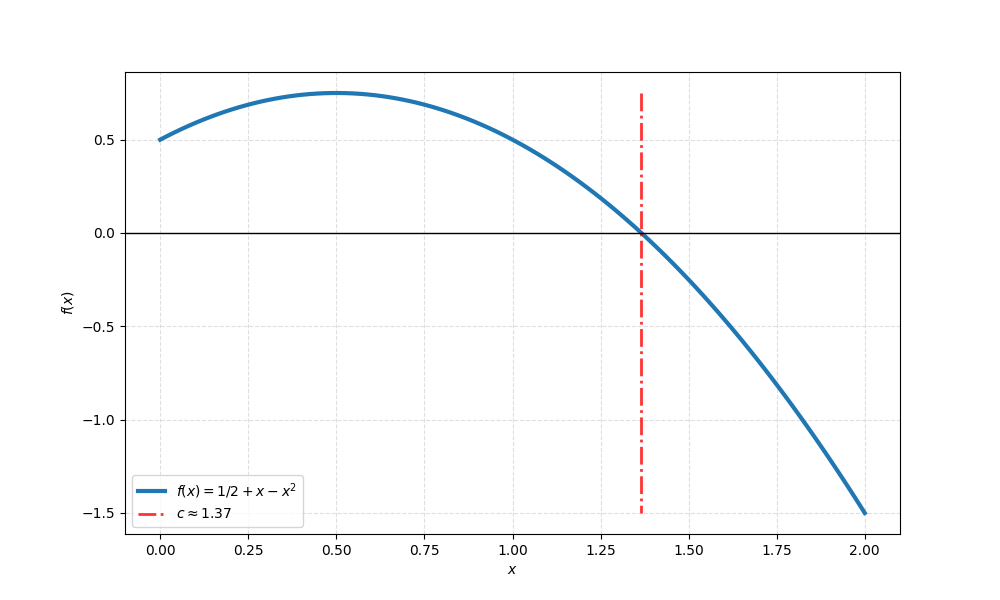
\includegraphics[width=0.8\linewidth]{images/12/plot_zero.png}
    \caption{Ricerca dello zero per $f(x)$}
    \label{fig: Zero bisec}
\end{figure}

\bigskip

\noindent Per quanto riguarda la convergenza di \textit{Bisection} e \textit{Regula Falsi}, accennavamo nel paragrafo precedente a come ci aspettiamo sia differente la velocità di convergenza alla soglia dei due algoritmi (sottolineando che però il rate rimane uguale per entrambi, essendo, sostanzialmente, lo stesso algoritmo con convergenza lineare): vogliamo in questa sezione mostrare questo comportamento con una rappresentazione dell'errore numerico e della distanza tra la \textit{guess} al passo n-esimo e il valore finale.

\medskip
\noindent Di seguito i grafici relativi ai due algoritmi: per ciascuno vediamo rappresentato sulla sinistra la convergenza della funzione, valutata nella \textit{guess}, allo zero matematico 
$$|f(c_n) - f(c_{true})| = |f(c_n) - 0| = |f(c_n)|$$
sulla destra troviamo la distanza n-esima della \textit{guess} da $c_{true}$, cioè l'errore al passo n-esimo
$$|c_n - c_{true}|=|c_n - \frac{1 + \sqrt{3}}{2}|$$

\medskip
\noindent La Fig. \ref{fig: Bis conv}, mostra il previsto andamento lineare di entrambi gli algoritmi: per quanto riguarda bisezione, l'andamento è caratterizzato da oscillazioni locali rispetto alla pendenza media. Al contrario, per Regula Falsi, si osserva come l'algoritmo mantenga l'ordine di convergenza  ma proceda in modo monotono: ogni iterazione riduce effettivamente la distanza dal valore vero. Nella bisezione, invece, la convergenza è garantita globalmente ma non è necessariamente decrescente passo dopo passo; può infatti accadere che:
$$\exists n \in [0, N_{max}] : |c_{n+1} - c| > |c_n - c|$$

\noindent Questa differenza riflette l'ottimizzazione introdotta dalla Regula Falsi: la scelta della \textit{guess} basata sull'interpolazione lineare risulta più efficace, specialmente su intervalli ridotti e per funzioni sufficientemente regolari. Il risultato è un processo di convergenza più "liscio" e rapido, pur restando nell'ambito della linearità.

\begin{figure}[H]
    \centering
    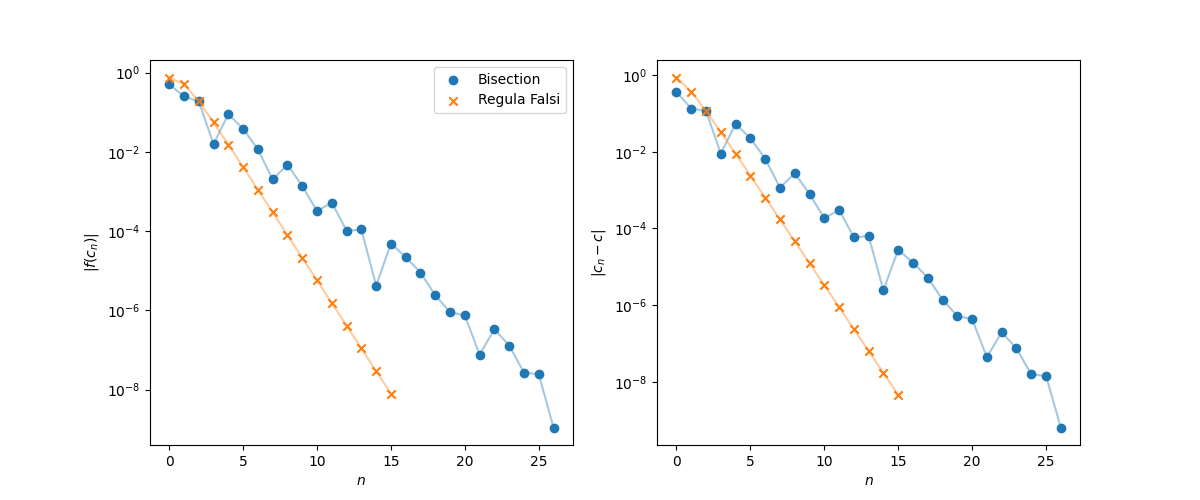
\includegraphics[width=\linewidth]{images/12/bis_vs_reg.png}
    \caption{Convergenza in funzione del numero di iterazioni dell'algoritmo di Bisezione e di Regula Falsi, per la funzione (sinistra) e il valore della radice (destra).}
    \label{fig: Bis conv}
\end{figure}

\noindent Con due fit dimostriamo, in Fig. \ref{fig: fit Bis} e Fig. \ref{fig: fit reg}, che l'andamento è lineare (fit su una retta di $\log(e_{k+1}) = \log(C) + p\log(e_k)$, con $p \approx 1$ per entrambe, dai risultati del fit). Da ora in avanti, quando ci si riferisce ai risultati di un fit per la convergenza di un algoritmo, valgono tutte le considerazioni che sono esplicitate e ampliate nell'Appendice (\hyperref[App: funzione fit]{App.1}) e sarà evitata la ripetizione delle stesse (vedi appunti sull'errore statistico dei risultati e setup del fit con forma logaritmica)

\begin{figure}[H]
    \centering
    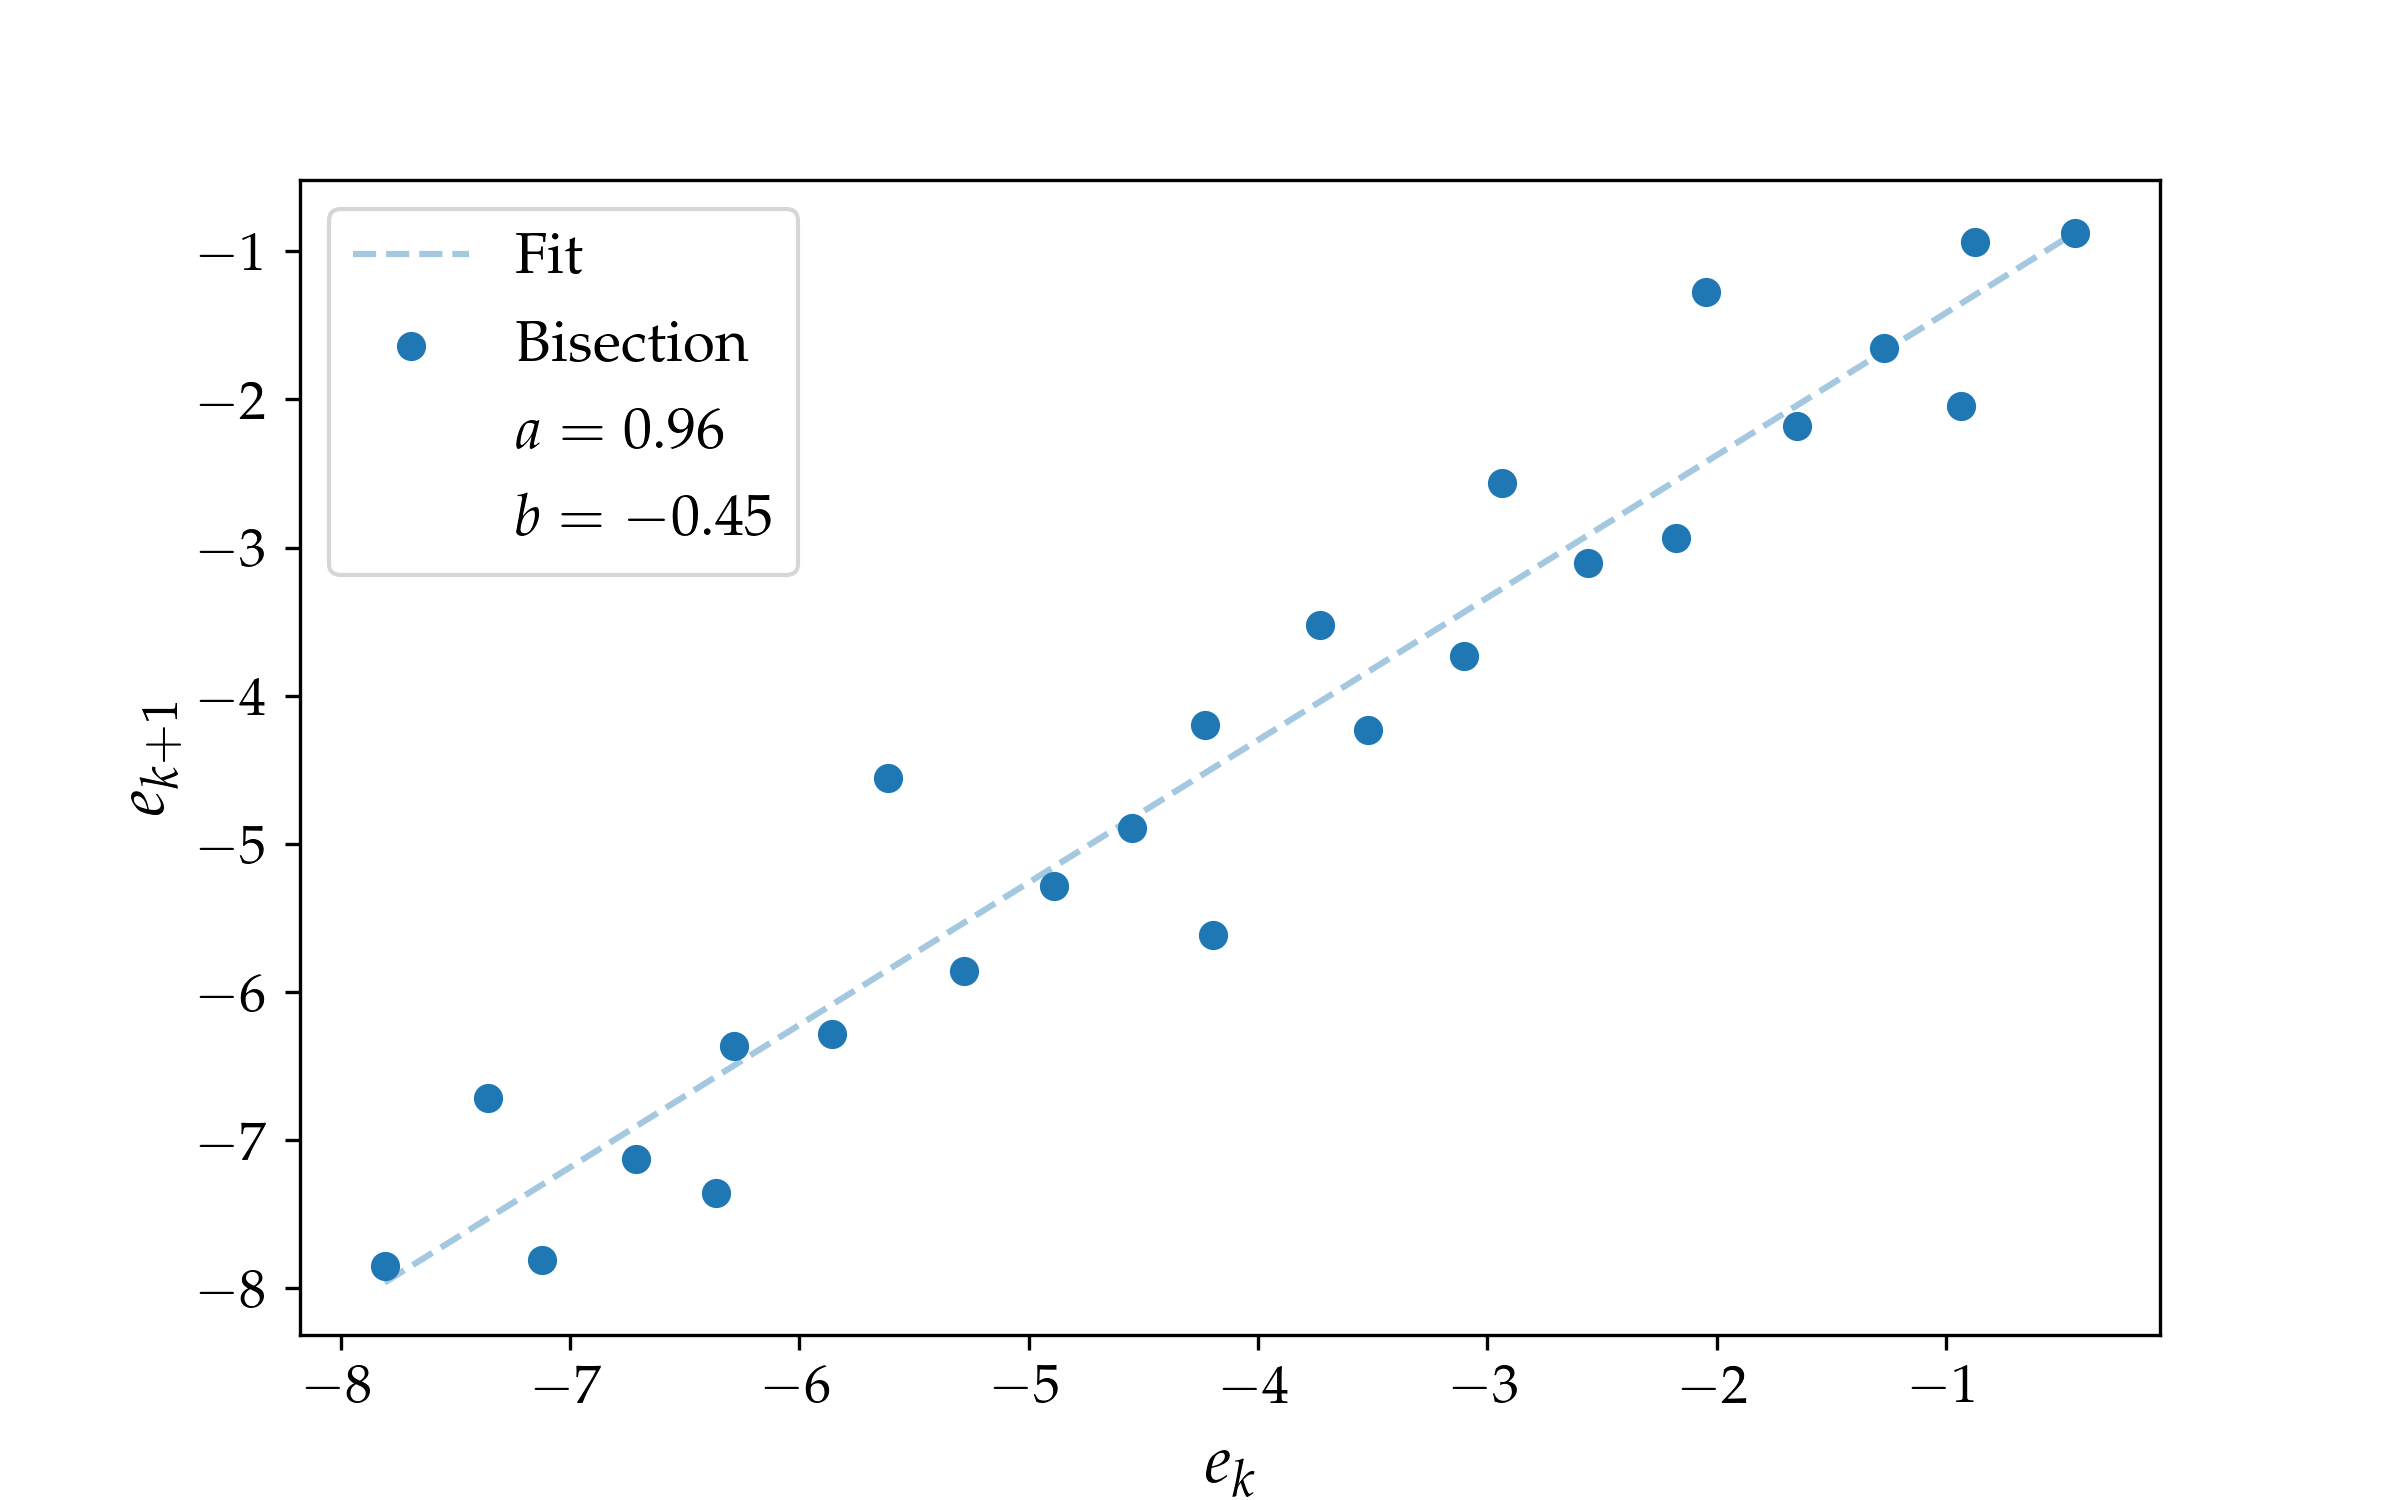
\includegraphics[width=0.8\linewidth]{images/12/fit_Bisection.png}
    \caption{Convergenza in funzione del numero di iterazioni dell'algoritmo di Bisezione. $e_k$, $e_{k+1}$ sono in realtà il $\log_{10}(e_i)$, abbreviato per semplicità con la formula senza il log: sull'asse sono indicate quindi le potenze del 10 a cui si riferiscono le grandezze.}
    \label{fig: fit Bis}
\end{figure}

\begin{figure}[H]
    \centering
    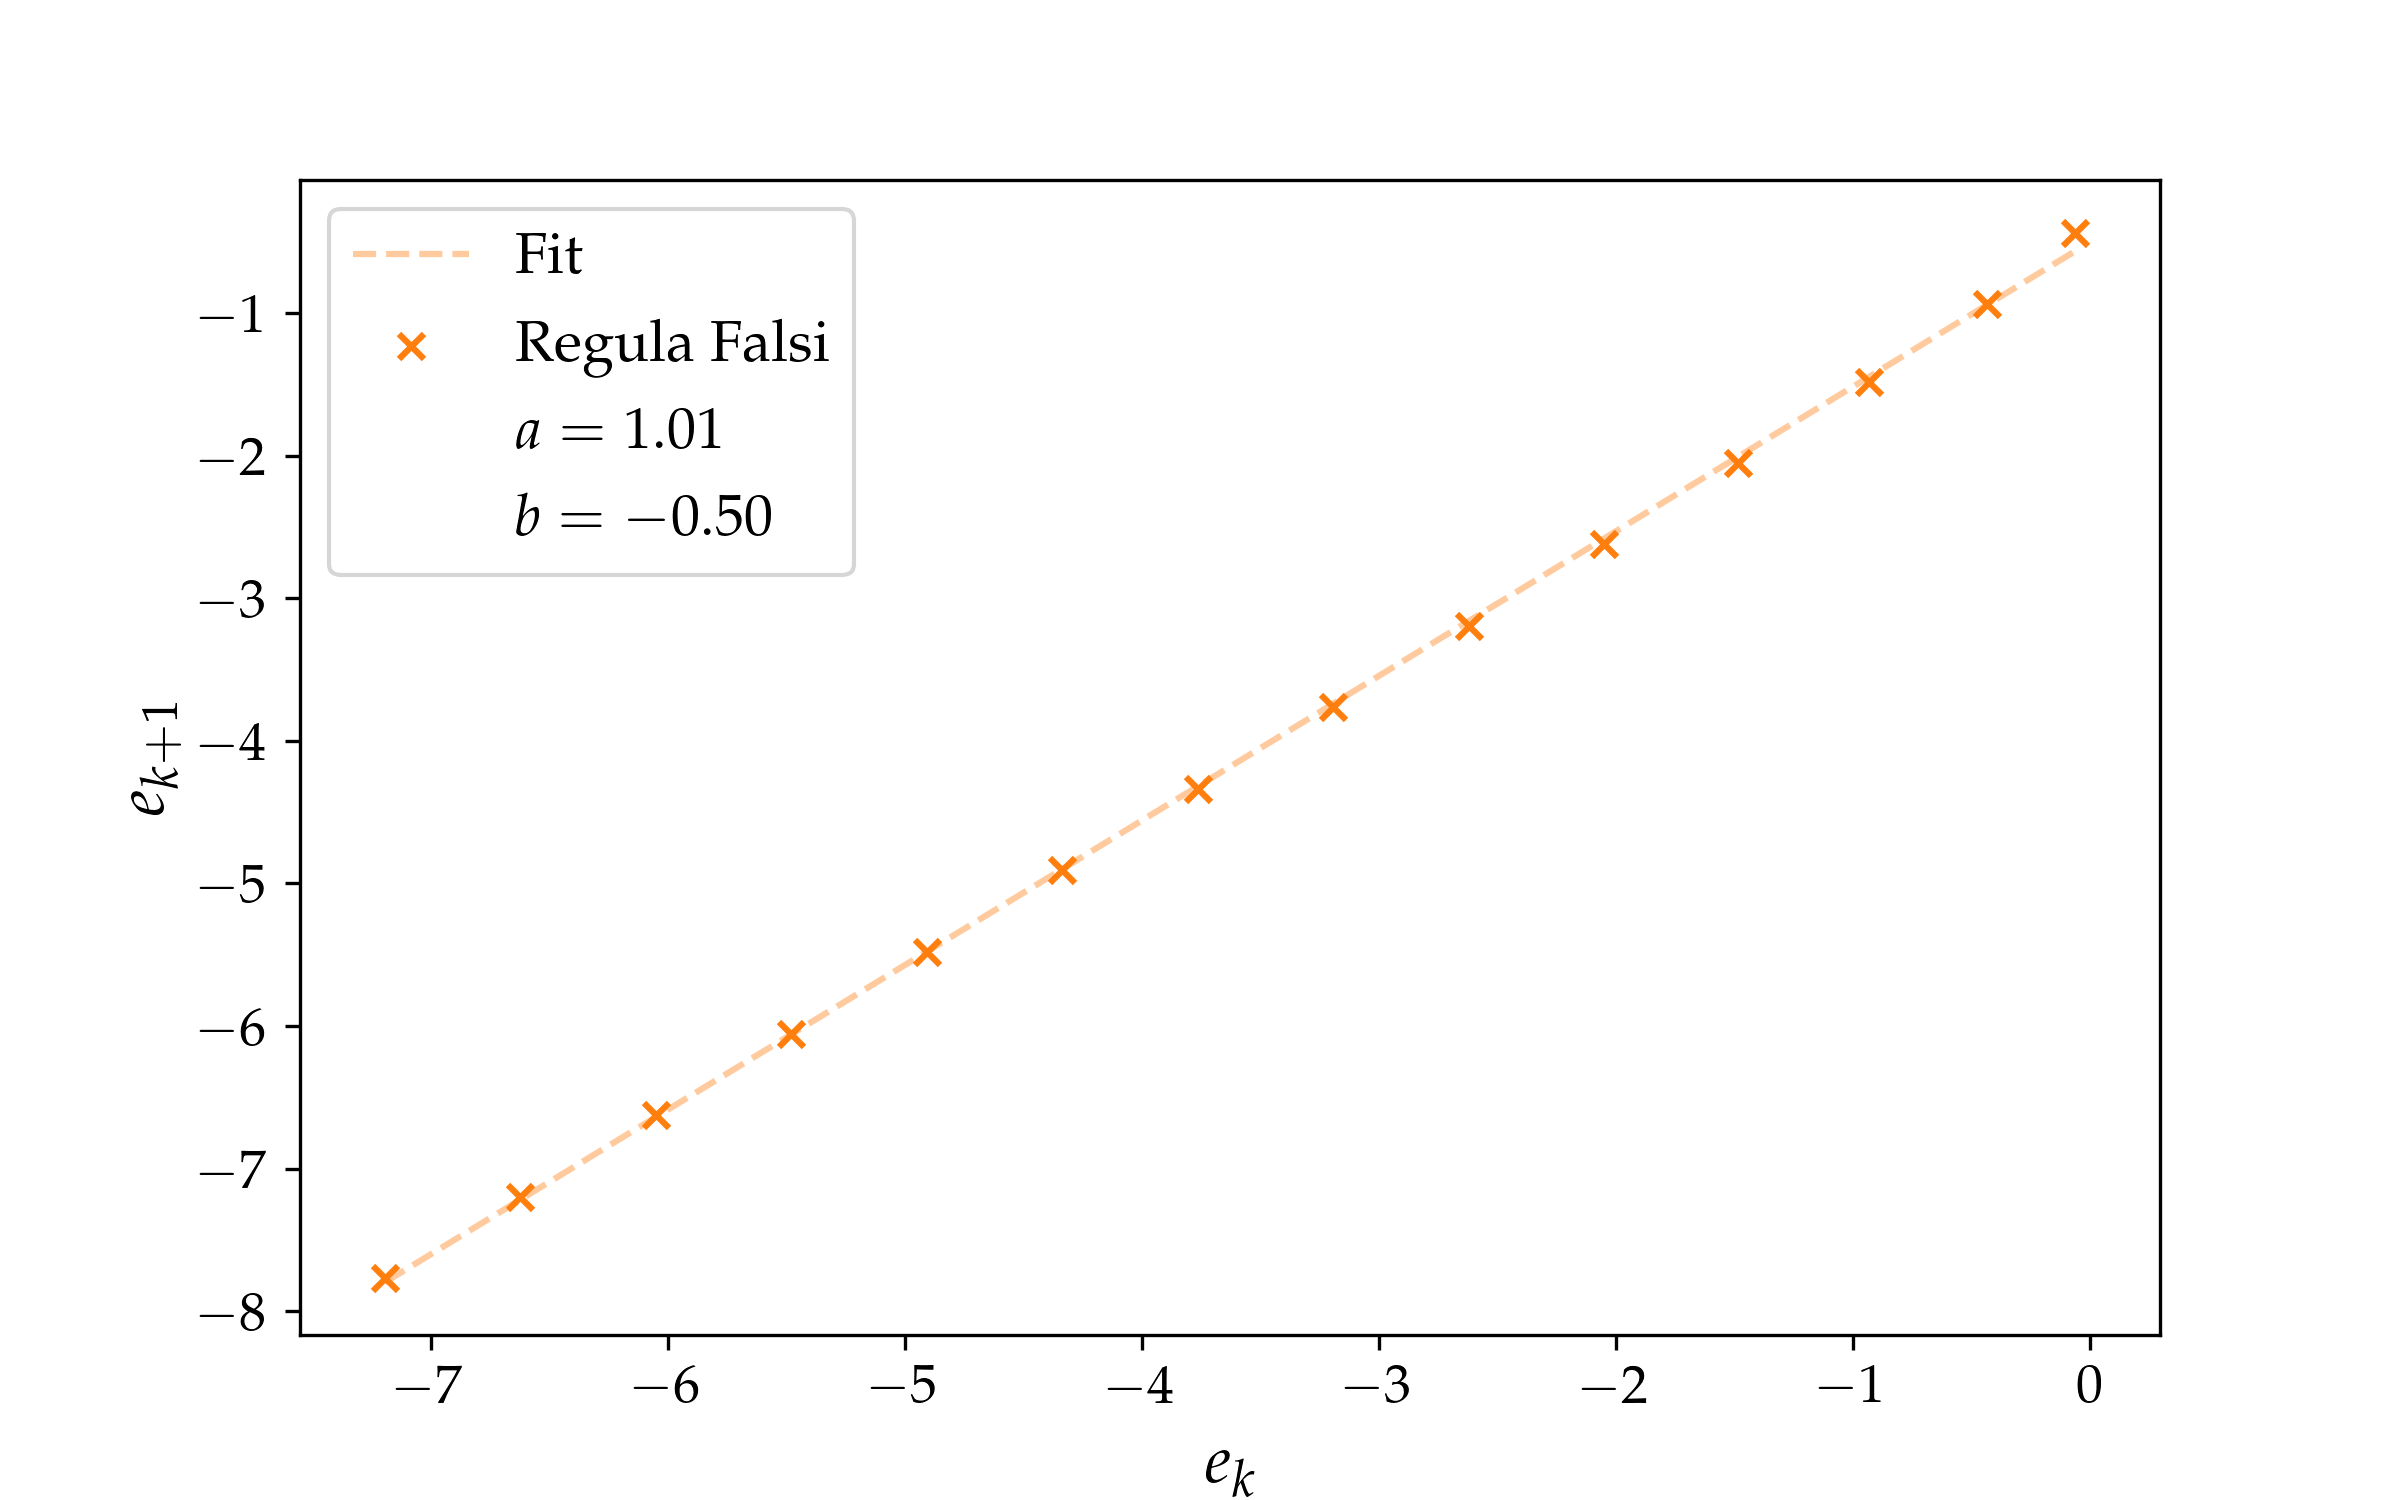
\includegraphics[width=0.8\linewidth]{images/12/fit_Regula_Falsi.png}
    \caption{Convergenza in funzione del numero di iterazioni dell'algoritmo di Regula Falsi. Per l'intestazione degli assi vale la stessa approssimazione del grafico sopra.}
    \label{fig: fit reg}
\end{figure}

\newpage










\section{Esercizio 5.1.2}
\subsection{Problem Statement}
Risolvi l'equazione di Keplero
\begin{equation} \label{eq: Keplero}
    M(t) = E(t) - e \sin(E(t))
\end{equation}

impostando i parametri $e = 0.5, a = 1$. Adotta la seguente regola per l'anomalia media $M(t) = 0.5t$.

\begin{enumerate}
    \item calcola il periodo $T$ da $E(T) = 2\pi$.
    \item prendi l'intervallo $t \in [0, T]$ e dividilo in 100 passi. Per ogni valore di $t$ calcola $E(t)$ trovando la radice dell'Eq. \ref{eq: Keplero} (usa il metodo della Regula Falsi) e le corrispondenti coordinate $x(t)$ e $y(t)$. Riporta i risultati in uno scatter plot.
    \item per un valore di $t$, studia la diversa convergenza in funzione del numero di iterazioni dei metodi della Regula Falsi e della bisezione.
\end{enumerate}

\subsection{Premessa Teorica}
Le \textit{Leggi di Keplero} descrivono le orbite ellittiche dei pianeti in rivoluzione attorno al sole. Rimanendo nel piano bidimensionale, esse sono definite come segue:

\begin{equation*} \label{eq: Kep Law}
    \begin{array}{ll}
    x(t) = a (\cos E(t)- e) \\
    y(t) = a \sqrt{1-e^2} \sin (E(t))
    \end{array}
\end{equation*}

\noindent dove introduciamo $0<e<1$, eccentricità dell'orbita e $E(t)$, anomalia eccentrica. Quest'ultima è legata dall'Eq. \ref{eq: Keplero} a $M(t)$, che definiamo anomalia media. 

\subsection{Metodi Numerici e Algoritmi}
Ci viene fornita la forma funzionale per $M(t) = 0.5t$: ciò permette di ricercare il valore di $E(t)$ per via numerica, semplicemente leggendo Eq. \ref{eq: Keplero} come
\begin{equation} \label{eq: root research}
M(t) - E(t) + e \sin(E(t)) = 0
\end{equation}

\noindent cioè trovando la radice di questa funzione $f(E(t))=0$. Due metodi di \textit{root finder} sono già stati implementati in Cap. \ref{sec. bisec e Regula Falsi} e saremo interessati al confronto dei loro risultati.

\bigskip
\noindent In primis troviamo il periodo dell'orbita, cercando $T$ in $E(T) = 2 \pi$:
\[
M(T) = 0.5T = E(T) - e  \sin(E(T)) = 2\pi
\]
\[
\implies T = 4 \pi
\]

\noindent Campionando l'intervallo $[0, T]$ con 100 valori valutiamo gli zeri t-esimi di Eq. \ref{eq: root research} (scegliamo di utilizzare il metodo \textit{Regula Falsi}), trovando $E(t)$ e risolvendo poi le \textit{Leggi di Keplero} per la determinazione delle coordinate $x(t), y(t)$.


\subsection{Risultati e Discussione}
La valutazione delle posizioni $x, y$ permette di disegnare l'orbita su un piano 2D: questa rappresentazione porta con sè anche alcune altre informazioni sulla dinamica del pianeta, per esempio dalla distanza dei marker possiamo visualizzare la velocità tangenziale del corpo
\footnote{
Le parti in cui la densità dei marker aumenta sono quelle in cui la velocità è minore, sapendo che i fotogrammi sono equispaziati nello span temporale. Possiamo notare come ciò avvenga nell'intorno della zona di massima curvatura. Si può osservare che per le parti con velocità maggiore vale il viceversa (e sarà interessata la zona speculare dell'orbita).}
. Nella Fig. \ref{fig: color_orbit} desideriamo mostrare proprio questo andamento, con un plot che, utilizzando una mappa di colore, rappresenta l'istante temporale a cui è riferita la posizione dello \textit{scatter plot}, cioè la posizione del pianeta sull'orbita in funzione del tempo.\\
Disegniamo una stella nella posizione di uno dei due fuochi ($x=y=0$): è semplice osservare che la velocità è massima nel punto di \textit{Perielio}, cioè quando la distanza tra il pianeta e la stella è minima, viceversa la velocità è minima per il punto di \textit{Afelio}, dove la distanza è massima.\\
La conferma e spiegazione di ciò è data dalla \textit{Seconda Legge di Keplero}, che afferma:
\begin{quote}
    ``Il segmento (raggio vettore) che unisce il centro del Sole con il centro del pianeta descrive aree uguali in tempi uguali.'' 
\end{quote}
È naturale concludere con le affermazioni che abbiamo enunciato a proposito della relazione tra massime e minime velocità e posizioni relative del pianeta nella sua orbita.\\
In particolare l'animazione "\textit{ani\_kep.mp4}", disponibile al link Github repo \url{https://github.com/mvolpato-unimib/Lab_comp/tree/main/ex12/plots}, 
è una chiara esemplificazione di ciò: ho unito nel plot la dinamica del pianeta sulla sua orbita e la rappresentazione dell'area spazzata dal raggio vettore in uno span di 30 istanti, mostrando che l'area rimane conservata e che la velocità cambia come abbiamo descritto precedentemente. 

\begin{figure}[H]
    \centering
    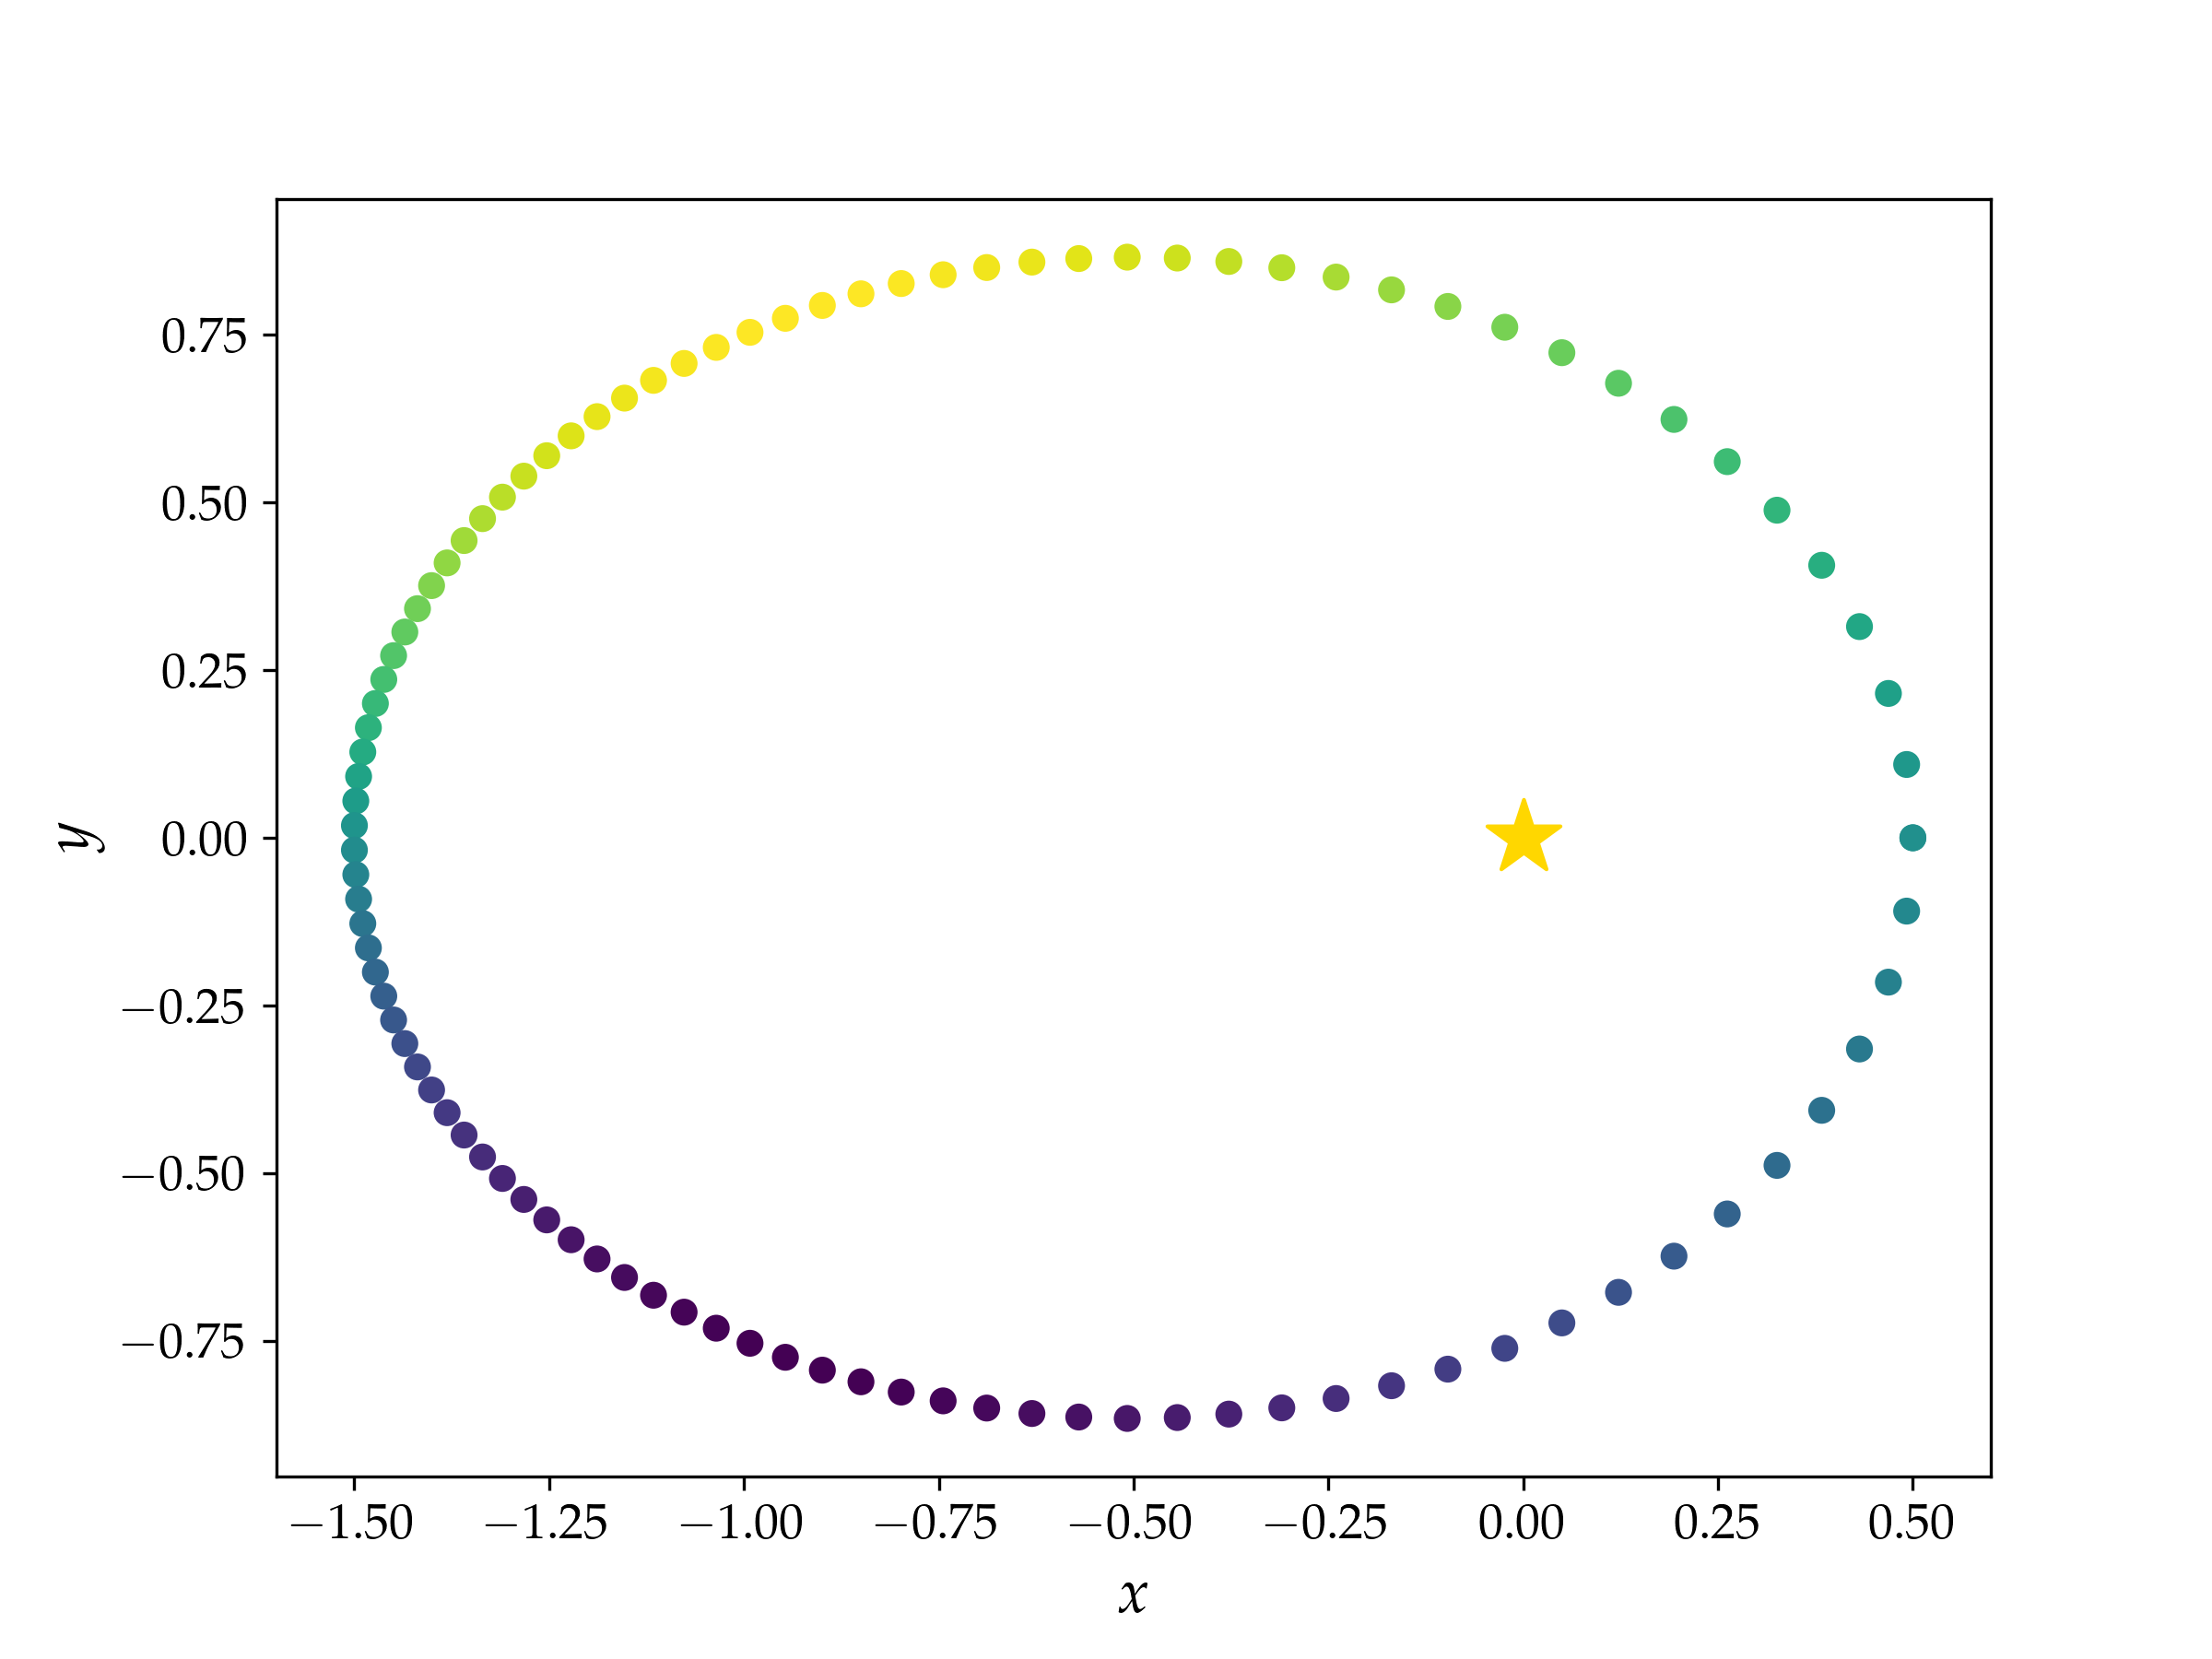
\includegraphics[width=0.8\linewidth]{images/12/color_orbit.png}
    \caption{Orbita del pianeta attorno al fuoco (stella). La mappa di colore indica l'istante temporale, da cui dipende la posizione del corpo.}
    \label{fig: color_orbit}
\end{figure}

\noindent Infine desideriamo confrontare come l'algoritmo di ricerca delle radici, in questo caso di default \textit{Regula Falsi}, abbia diversa convergenza in base al metodo. La discussione sarà del tutto simile a quella del Cap. \ref{sec: risultati bisec regula}, dove analizzavamo Fig. \ref{fig: Bis conv}. Rimettiamo al riferimento a quella sezione le specifiche dei plot, ma concludiamo che vengono confermate tutte le considerazioni precedenti: entrambi i metodi hanno convergenza lineare, ma con costanti di convergenza differenti, il che si riflette in un numero di iterazioni significativamente diverso.

\medskip
\noindent Fissato un valore di $t\in [0, T]$, scegliamo $t=1$, possiamo effettuare la ricerca della radice della funzione
\[
f(E(1)) = 0.5  - E(1) + e \cdot \sin(E(1)) = 0
\]
scegliamo un intervallo $I=[-1, 5]$, tale che $f(-1)\cdot f(5) < 0$ (per assicurare la presenza della radice), che servirà anche per inizializzare i due algoritmi. Plottiamo in Fig. \ref{fig: zero Kep} l'andamento della funzione nell'intervallo. 

\begin{figure}[H]
    \centering
    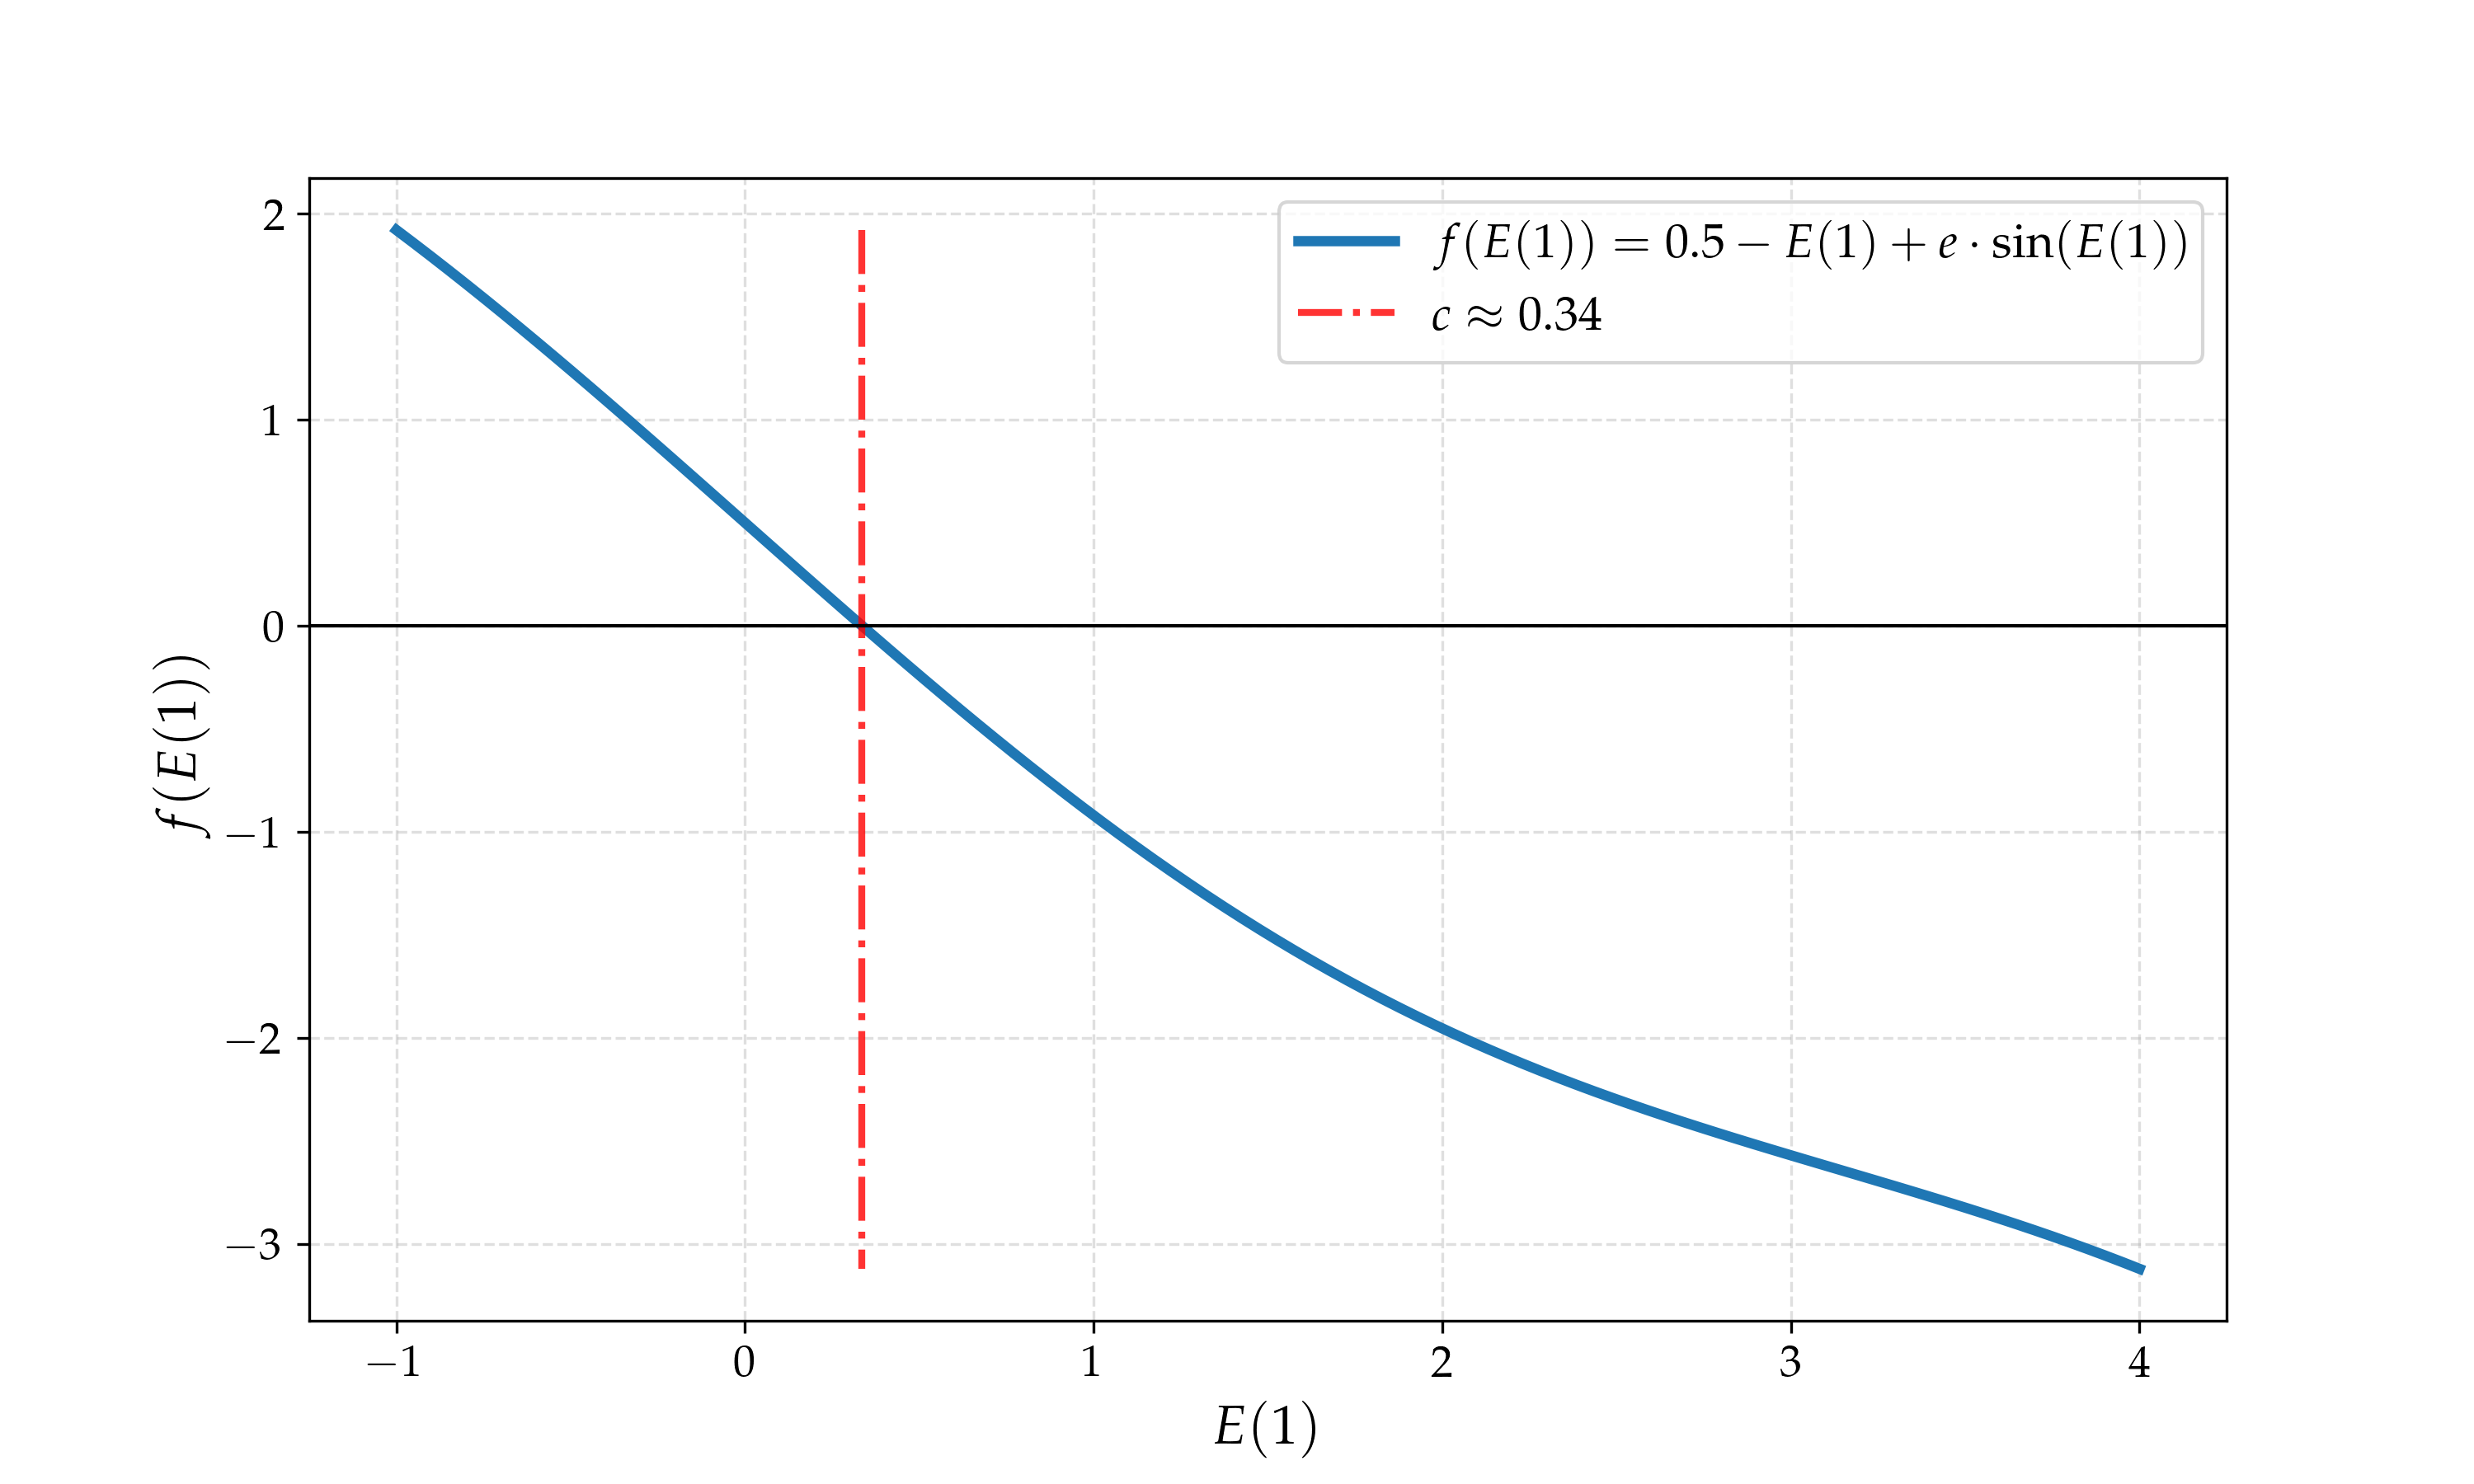
\includegraphics[width=0.8\linewidth]{images/12/plot_Kep_zero.png}
    \caption{Ricerca dello zero per $f(E(1))$.}
    \label{fig: zero Kep}
\end{figure}

Gli algoritmi restituiscono questi risultati:

\begin{elegantcode}
- BISECTION MTH
     Found f(c) = 0:  c =  0.3354180343449116
     N_iter =  29

- REGULA FALSI
     Found f(c) = 0:  c =  0.33541803238804735
     N_iter =  5

diff = 1.956864226215771e-09
\end{elegantcode}

\noindent Infine in Fig. \ref{fig: conv kep} la convergenza rispettivamente della funzione e dell'errore sulla radice e il controllo dell'ordine (aspettato lineare e verificato, $a\approx1$) con un fit sui dati del caso di bisezione (Fig. \ref{fig: kep fit bis}).

\medskip
\noindent
Si noti che se dai risultati del metodo si può leggere che il numero di iterazioni è stato di $n_{iter}=5$ per Regula Falsi, i punti sui grafici sono quattro; questo perché il confronto per valutare l'errore viene fatto sull'ultimo punto valutato, preso di riferimento come valore vero: di conseguenza $n \in [0, N_{iter}-1]$.\\

\medskip \noindent
Manca il grafico relativo al fit dell'algoritmo di Regula Falsi, poiché il confronto $e_k$ vs $e_{k+1}$ riduce i punti: inizialmente abbiamo $e_k = (e_1, \dots, e_{n-1})$, decidendo di non considerare l'ultimo elemento, costruiamo $e_{k+1} = (e_2, \dots, e_{n-1})$, abbiamo così definito una coppia di vettori che confrontati rappresentano le coppie di errori ad un passo $k$ e $k+1$.\\
Nel caso specifico, con $N_{iter} = 4$, abbiamo: 
\begin{align*}
e_k &= (e_1, \dots, e_{n-2}), \\
e_{k+1} &= (e_2, \dots, e_{n-1}) \\
&\xrightarrow{\text{ }} e_k = (e_1, e_2), \\
&\xrightarrow{\text{ }} e_{k+1} = (e_2, e_3)
\end{align*}

\noindent Si ottiene un fit con solo due punti, non significativo per una analisi dell'andamento da studiare: non è quindi stato incluso alcun grafico per il fit di questo secondo metodo.

\begin{figure} [H]
    \centering
    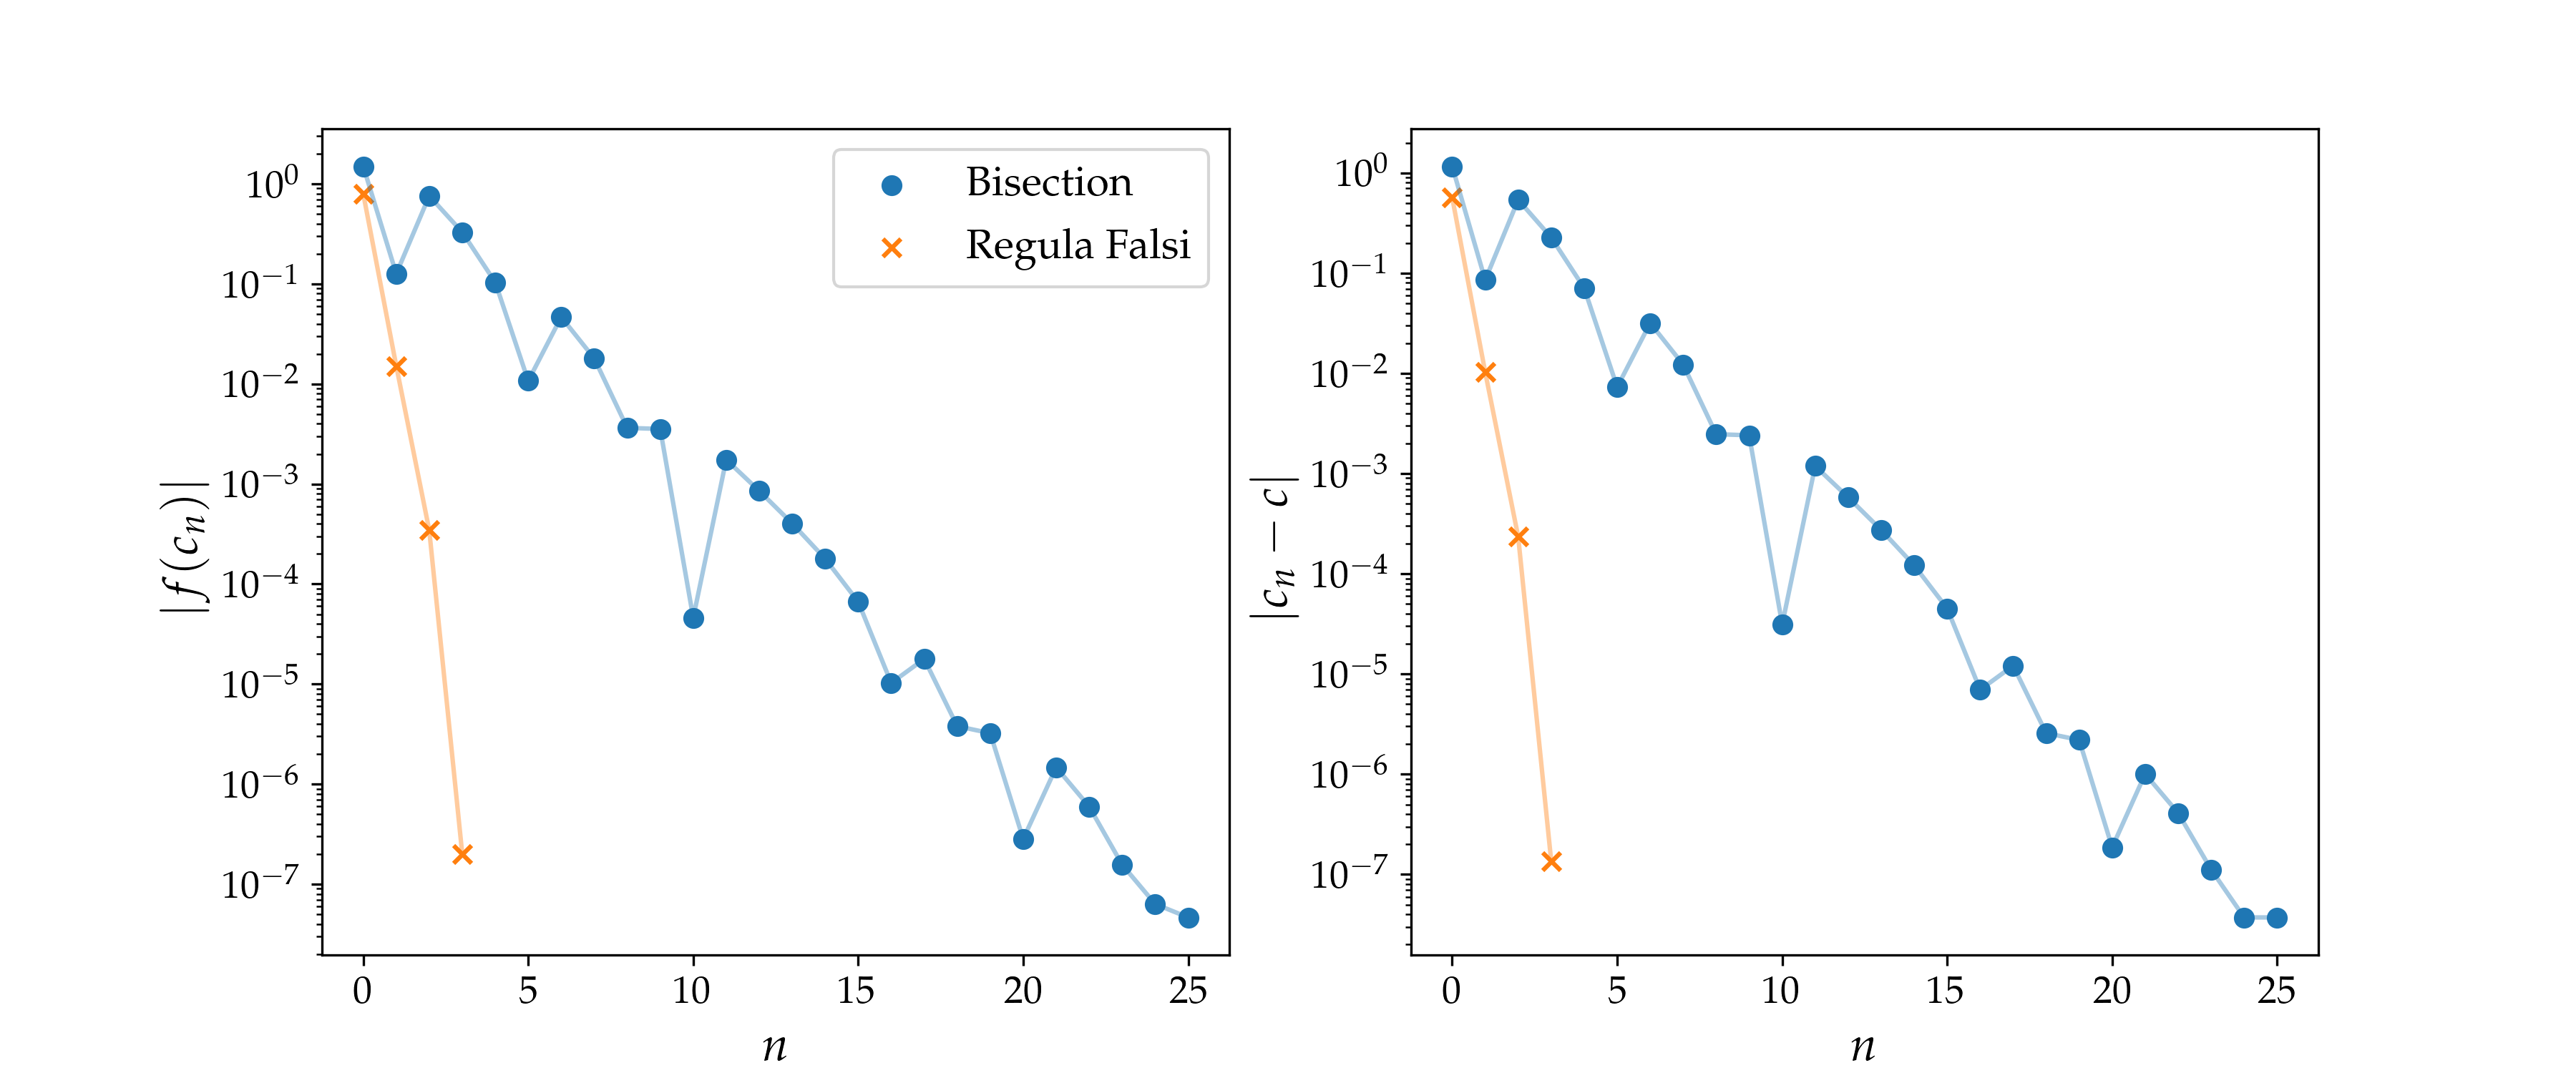
\includegraphics[width=\linewidth]{images/12/bis_vs_reg_keplero.png}
    \caption{Confronto della convergenza in funzione del numero di iterazioni dell'algoritmo di Bisezione vs Regula Falsi  per la funzione (sinistra) e il valore della radice (destra).}
    \label{fig: conv kep}
\end{figure}

\begin{figure} [H]
    \centering
    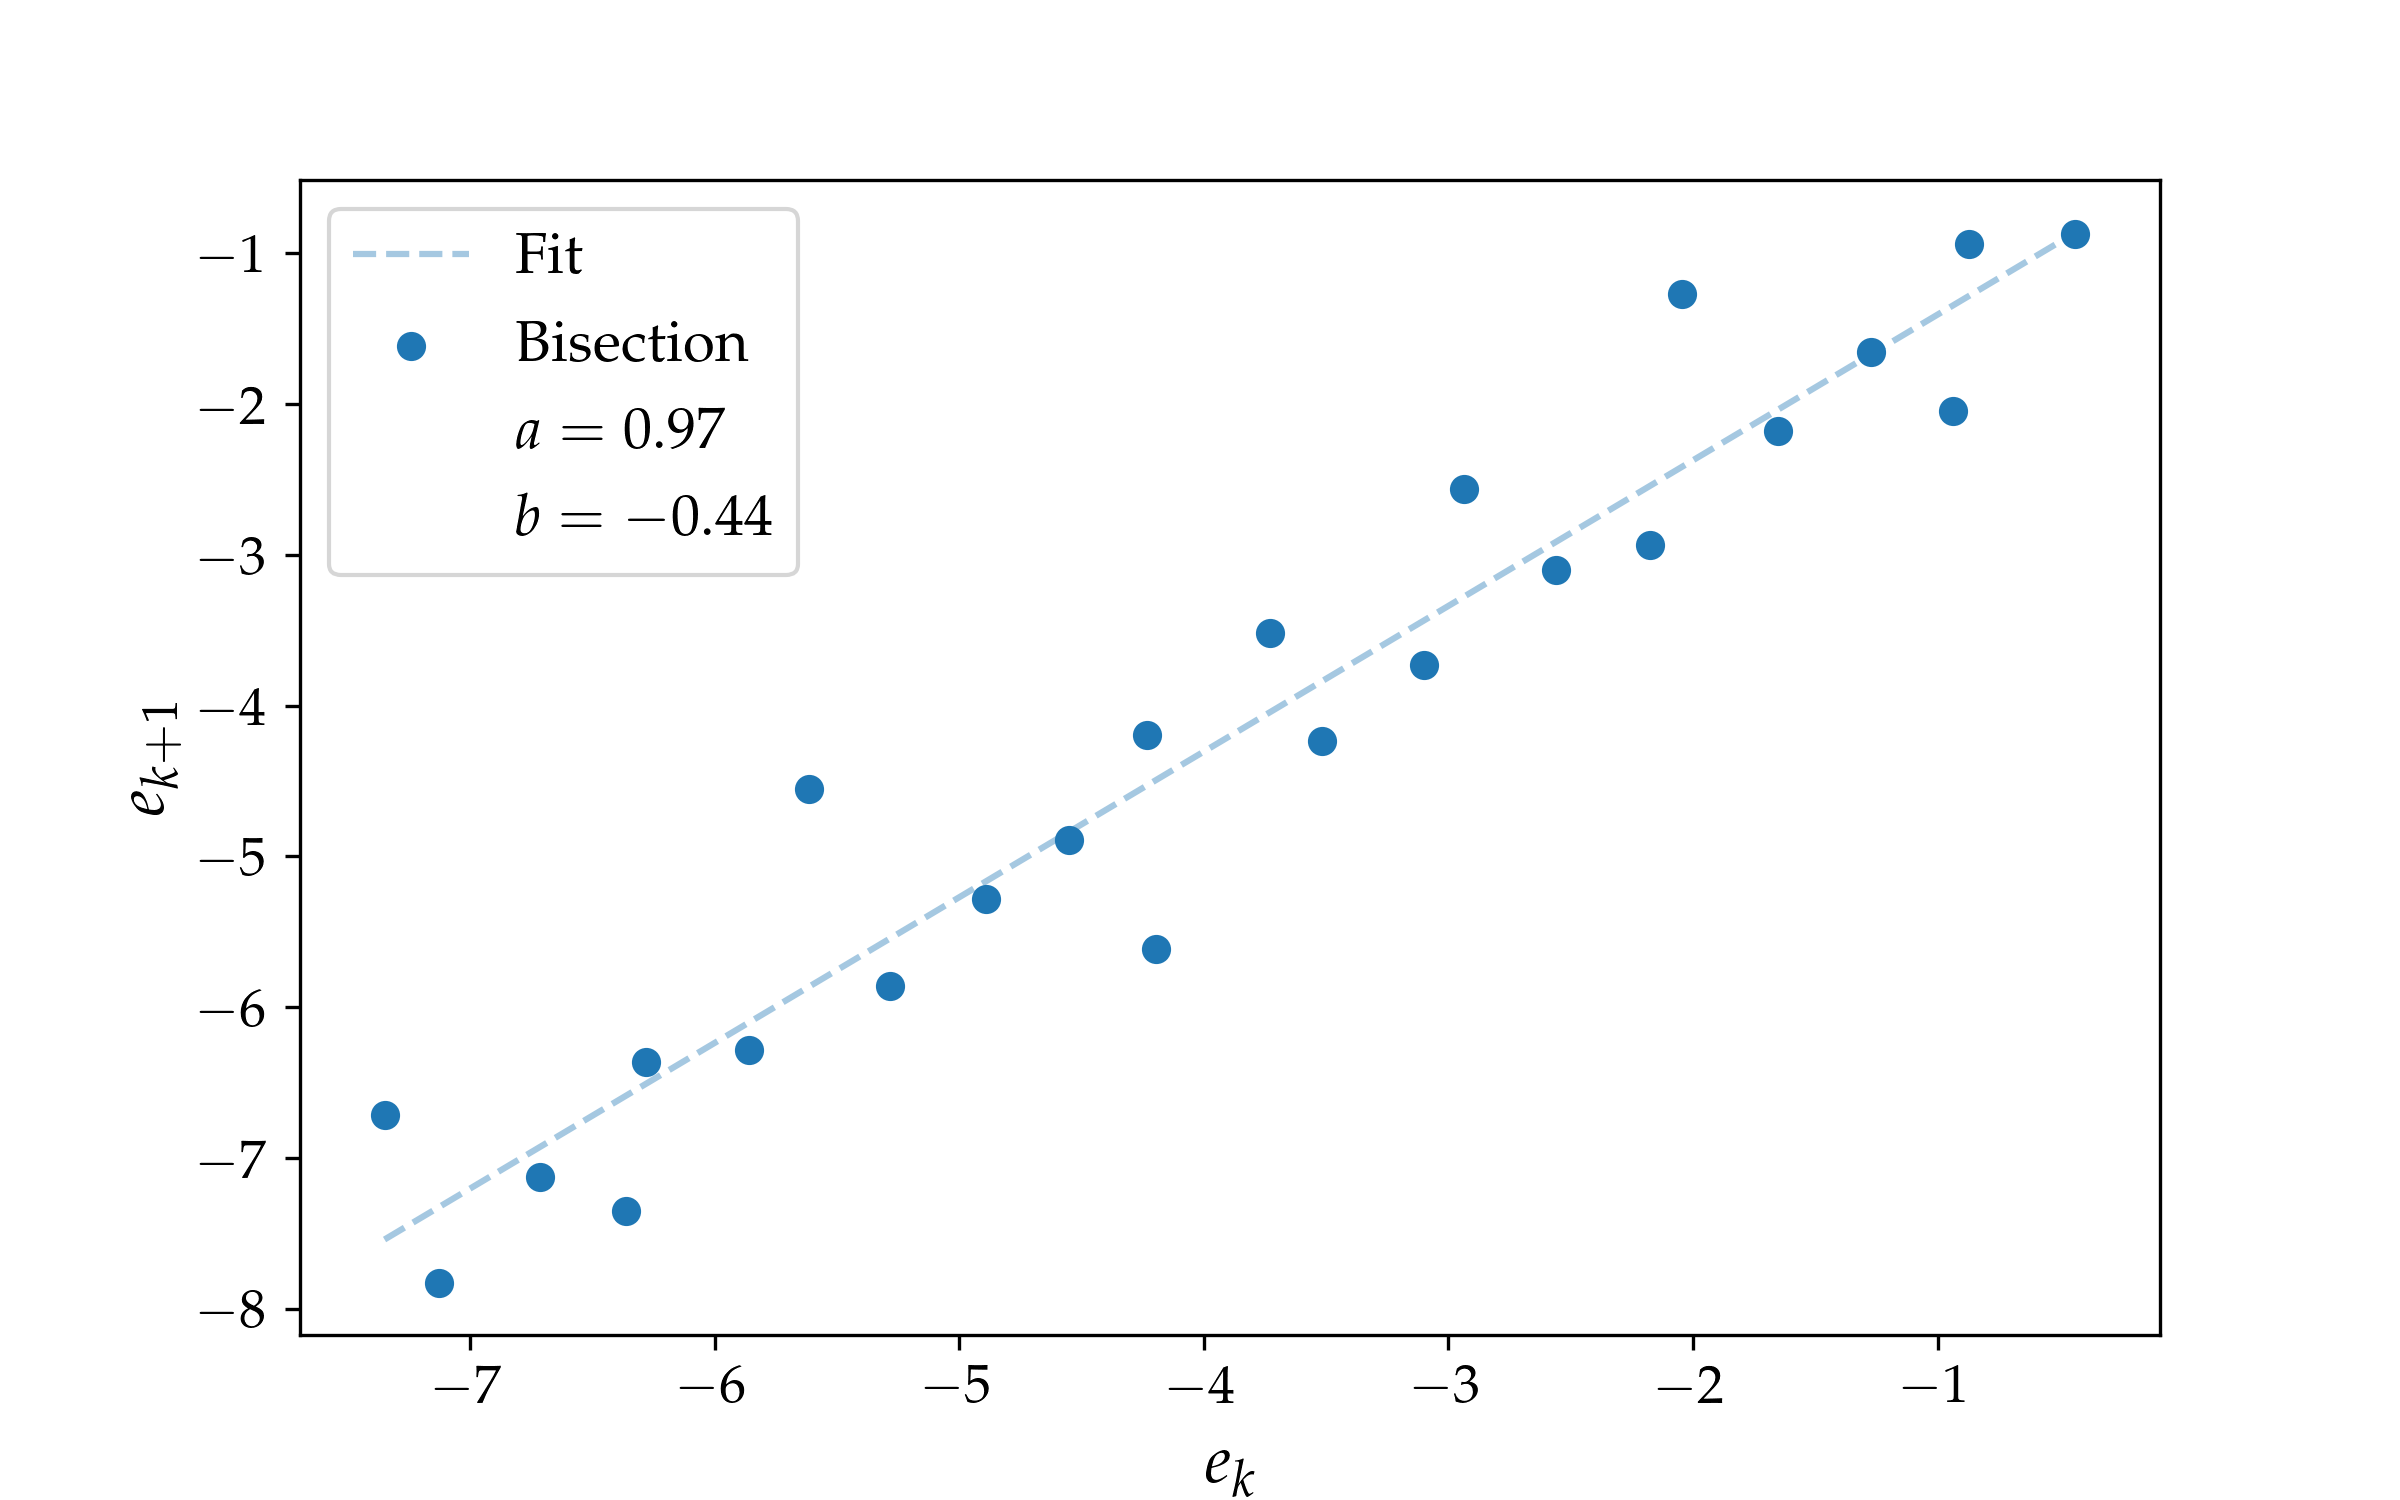
\includegraphics[width=0.8\linewidth]{images/12/keplero_fit_Bisection.png}
    \caption{Convergenza in funzione del numero di iterazioni dell'algoritmo di Bisezione. Per l'intestazione degli assi vale la stessa approssimazione di Fig. \ref{fig: fit Bis}.}
    \label{fig: kep fit bis}
\end{figure}

\newpage






\section{Esercizio 5.2.1}

\subsection{Problem Statement}
Scrivete una funzione che implementi l'algoritmo di Newton e studiate i tre casi seguenti, che dovrebbero illustrare i problemi di questo metodo.

\subsection*{1. Convergenza lenta}
Considerate la funzione $f(x) = x^2$ e calcolate la sua radice con l'algoritmo di Newton-Raphson, partendo da $x_0 = 0.8$. La convergenza è quadratica? Spiegatelo utilizzando sia evidenze analitiche che quelle numeriche.

\subsection*{2. Cicli}
In alcuni casi il metodo di Newton non converge mai poiché, a causa di una commissione tra la funzione e l'ipotesi iniziale, l'algoritmo entra in un ciclo infinito. Considerate la funzione $f(x) = x^3 - 2x + 2$ e le ipotesi iniziali $x_0 = 0$ e $x_0 = 1$. Tracciate i valori della radice $x_n$ in funzione di $n$. Perché oscilla tra 0 e 1? Una volta compreso il meccanismo, trovate una soluzione.

\subsection*{3. Condizioni iniziali}
L'algoritmo di Newton può essere molto suscettibile alle condizioni iniziali, in particolare se scegliamo un'ipotesi iniziale (o se finiamo per trovarci su un punto) in cui la derivata prima è molto vicina a zero. Ciò può portare a un grande salto in una singola iterazione, che manda l'algoritmo in una regione più vicina a una soluzione diversa rispetto a quella che stavamo affrontando.

\medskip

Per illustrare il problema della forte sensibilità alle condizioni iniziali, immaginiamo di dividere un certo dominio in un insieme discreto di punti, applicare l'algoritmo di Newton a ciascun punto per una data funzione che ammette almeno 2 radici e poi vedere a quale radice converge ciascun punto. Successivamente, possiamo assegnare un colore a ogni soluzione e mappare la sensibilità alle condizioni iniziali sotto forma di confini tra aree di colori diversi.

Consideriamo i numeri complessi e prendiamo la funzione

$$f(z) = (z^2 - 1)(z^2 + 1)$$

con quattro radici $1, -1, i, -i$. Per assegnare un colore a ogni radice, calcolate semplicemente l'angolo in coordinate polari della soluzione corrispondente.

Successivamente, create una griglia di punti nel piano complesso bidimensionale, dove la densità della griglia specifica il numero di \textit{pixel} che abbiamo.



\subsection{Premessa Teorica}
Abbiamo già presentato due esempi di algoritmi che sono definiti \textit{bracketed}, cioè per cui l'inizializzazione del metodo è legata alla definizione di un intervallo in cui assicuriamo la convergenza. Questo punto di forza è bilanciato dall'ordine di convergenza, lineare, che limita il loro utilizzo. \\
L'algoritmo di Newton-Raphson offre un'altra possibilità: ci permette di migliorare la convergenza rispetto al \textit{metodo di bisezione} (o \textit{Regula Falsi}) passando ad uno scaling quadratico; paghiamo sulla robustezza del metodo, che non assicura più la convergenza, dato un certo punto $x_0$ con cui inizializzare. 

\subsection{Metodi Numerici e Algoritmi}
Il metodo di N-R è definito come segue:\\
data la funzione $f$ e supponendo esista una sua radice $L$ nel nostro dominio di ricerca ($f(L)=0$), è possibile definire l'algoritmo iterativo di \textit{Newton-Raphson} (N-R) 
\[
    x_{n+1} \equiv x_n - \frac{f(x_n)}{f'(x_n)}
\]

\noindent Da questa definizione si può dimostrare che l'errore al passo n-esimo è dato da:
\[
    L - x_{n+1} = - \frac12 \frac{f''(L)}{f'(x_n)} (L-x_n)^2 + O((x_n-L)^3)
\]
cioè per una radice semplice ($f'(L) \not=0$) il metodo di Newton presenta convergenza quadratica. 
\medskip

\noindent Le problematiche di questo metodo sono legate al ruolo che giocano la derivata prima e seconda all'interno delle relazioni: il loro rapporto può accelerare o rallentare fortemente l'algoritmo e in particolare un valore di $f'(x) \approx 0$ potrebbe causare la non convergenza (questo termine si trova al denominatore in entrambe le equazioni). Il vantaggio di aumentare la potenza di scaling è compensato dal pericolo di far fallire l'algoritmo lavorando con delle condizioni iniziali sconvenienti. 



\subsection{Risultati e Discussione}
\subsubsection{Convergenza lenta}
Seguendo la consegna, inizializziamo l'algoritmo con $x_0=0.8$, la funzione di test è $f(x)=x^2$:\\
la valutazione analitica della radice è $L=0$, notando che $f(L), f'(L)=0$. Ci aspettiamo di vedere un cambiamento nel fattore di scaling, come avevamo proposto nel paragrafo precedente e con alcuni passaggi analitici è possibile dimostrare ciò in forma generale.

\medskip
\noindent
Ripartendo con la definizione dell'algoritmo in forma iterativa:
\[
    x_{n+1} \equiv x_n - \frac{f(x_n)}{f'(x_n)}
\]
sviluppiamo $f(x_n), f'(x_n)$ con Taylor per $x_n = L$, cioè intorno alla nostra radice:
\begin{align*}
    f(x_n) &= f(L) + x_n f'(L) + \frac{x_n^2}{2}f''(L) + O(x_n^3)\\
    f'(x_n) &= f'(L) + x_n f''(L) + O(x_n^2)
\end{align*}
ricordando $f(L), f'(L)=0$:
\begin{align*}
    f(x_n) &= \frac{x_n^2}{2}f''(L) + O(x_n^3) = x_n^2 (\frac{1}{2} f''(L) + O(x_n))\\
    f'(x_n) &=x_n f''(L) + O(x_n^2) = x_n (f''(L) + O(x_n))
\end{align*}

\begin{align*}
\xrightarrow{}  x_{n+1} &=  x_n - \frac{x_n^2 (\frac{1}{2}f''(L) + O(x_n))}{x_n (f''(L) + O(x_n))} \\
&\approx  x_n - x_n \frac{\frac{1}{2}f''(L)}{f''(L)} \\
&\approx  x_n (1 - 1/2) 
\end{align*}

\[
x_{n+1} \approx\frac{1}{2} x_n
\]

risultato valido in forma generale per $f(L), f'(L)=0$: nel nostro caso:

\[
L=0 \implies x_i = |L-x_i| = e_i 
\]

La relazione finale, espressa in termini dell'errore al passo $n$:
\begin{align*}
\implies e_{n+1} &\approx\frac{1}{2} e_n \\
\implies \log_{10}(e_{n+1}) &\approx \log_{10}(e_n) + \log_{10}(1/2)  \\
\end{align*}

\noindent In particolare di seguito nella forma utilizzata per il fit e una stima dei parametri attesi con questa derivazione analitica: 
\begin{align*}
\implies \epsilon_{n+1} &\approx a\cdot \epsilon_{n} + b\ \\
\epsilon_i =\log_{10}(e_i),\ a&=1,\ b =  \log_{10}(1/2) \approx -0.3
\end{align*}

\noindent Ciò che vogliamo confermare con questo esempio è che il metodo, con le appropriate condizioni iniziali, può modificare il suo \textit{scaling}, non riproducendo un carattere quadratico, ma, come è reso evidente in questo caso, un andamento lineare nell'ordine di convergenza.\\

\medskip\noindent
In Fig. \ref{fig: N-R lin repr} una rappresentazione delle radici trovate sulla funzione di test al variare del numero di interazioni, in Fig. \ref{fig: fit NR lin} il fit della funzione, dove si noti che i parametri stimati numericamente coincidono con i risultati analitici.

\begin{figure}[H]
    \centering
    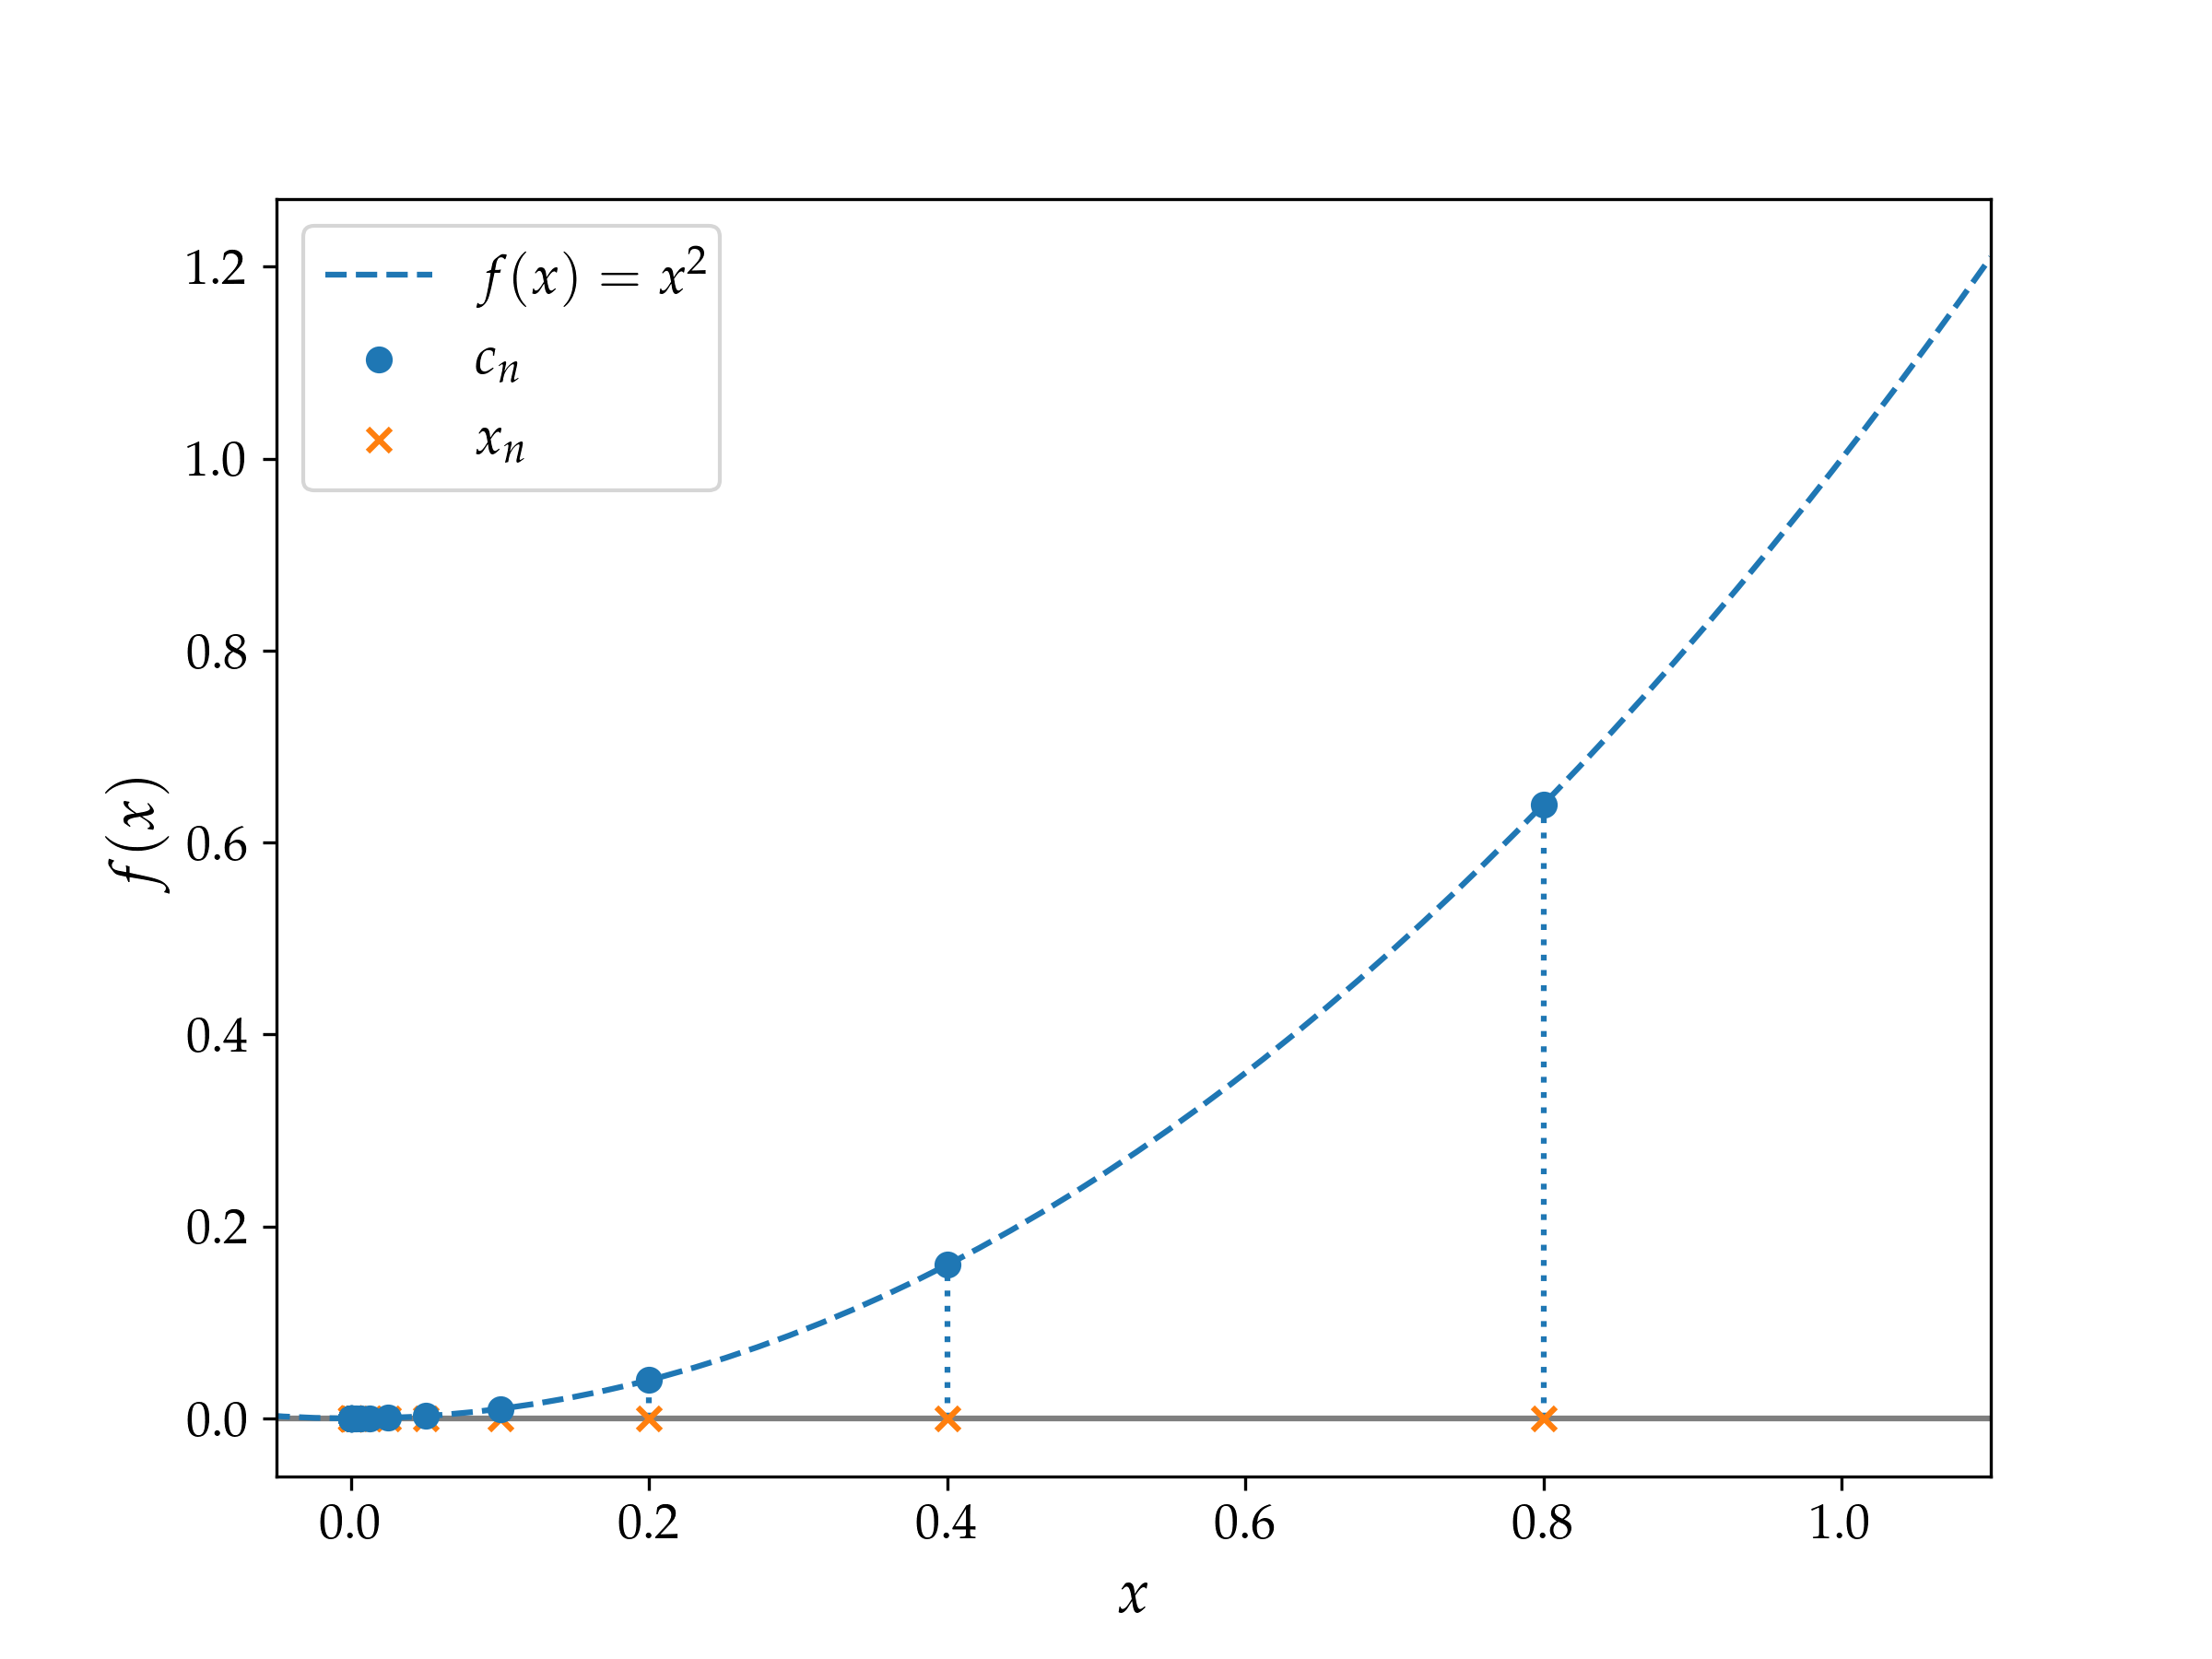
\includegraphics[width=0.7\linewidth]{images/13/init_cond.png}
    
    \caption{I risultati dell'algoritmo N-R con la funzione $f(x)= x^2\ ,\ x_0=0.8$: $x_n$ rappresentano le radici al passo n-esimo, dove si può osservare la convergenza al valore analitico di $x=0$, i $c_n$ sono invece i punti $(x_n, f(x_n)).$}
    \label{fig: N-R lin repr}
\end{figure}

\begin{figure}[H]
    \centering
    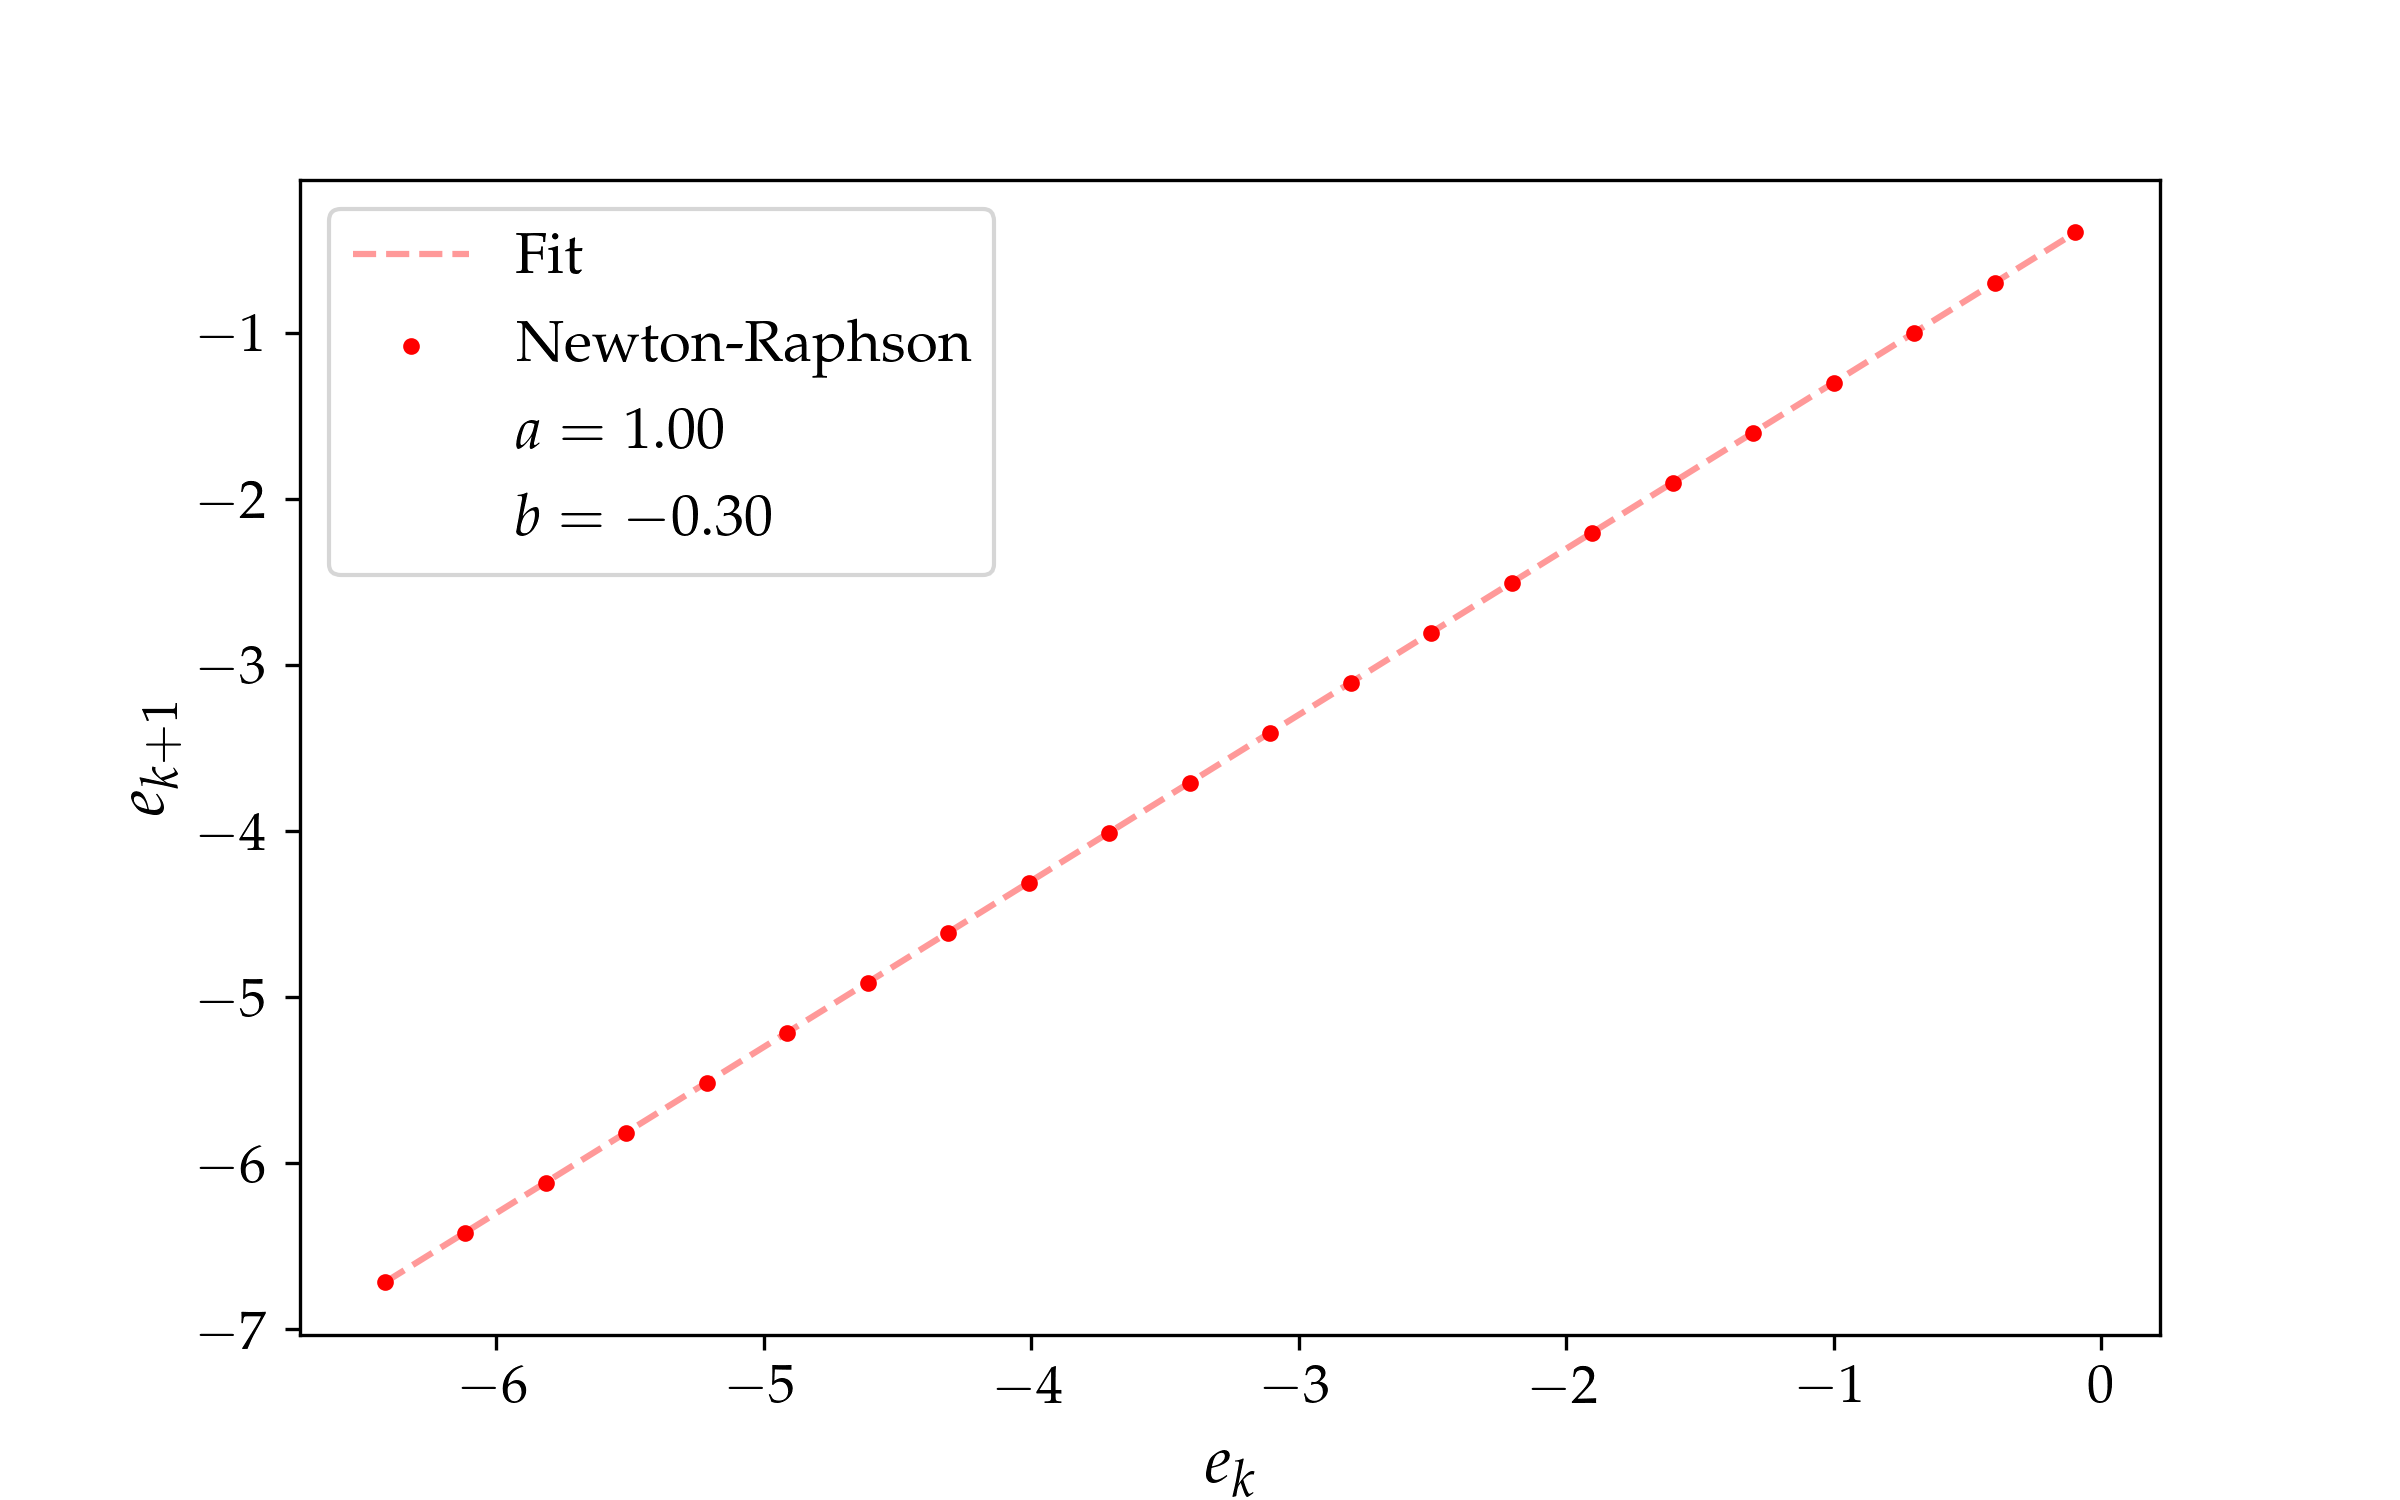
\includegraphics[width=0.8\linewidth]{images/13/fit_NR_lin.png}
    
    \caption{Convergenza in funzione del numero di iterazioni dell'algoritmo di Newton-Raphson. Per l'intestazione degli assi vale la stessa approssimazione di Fig. \ref{fig: fit Bis}.}
    \label{fig: fit NR lin}
\end{figure}


\subsubsection{Cicli}
Il secondo caso che analizziamo è quello della funzione 
\[
f(x) = x^3 -2x + 2
\]
La richiesta è di studiare l'andamento con condizioni iniziali $x_0 = 0$ e $x_0 = 1$, verificando che il metodo oscilla indefinitivamente tra i due valori, senza mai convergere alla soluzione.\\ 
L'analisi che propongo studia il comportamento in funzione di $x_0 \in [0, 1]$, estremi inclusi, osservando come per punti intermedi il metodo converga, e per i due limiti si osservi il fenomeno descritto nella consegna:\\
la soluzione analitica è:

\[
x = \sqrt[3]{-1 + \frac{\sqrt{57}}{9}} + \sqrt[3]{-1 - \frac{\sqrt{57}}{9}} \approx -1.7693
\]

\noindent In Fig. \ref{fig: NR conv 0,1} una chiara rappresentazione del fenomeno.

\medskip\noindent
Una semplice spiegazione può essere data osservando la definizione analitica dell'algoritmo e studiando cosa accade per $x_0=0,1$.\\
\begin{align*}
    f(x) &= x^3 - 2x +2\ \quad\quad
    \begin{cases}
    f(0) = 2 \\
    f(1) = 1
    \end{cases}\\
    f'(x) &= 3x^2 - 2 \quad\quad\quad\quad 
    \begin{cases}
    f'(0) = -2 \\
    f'(1) = 1
    \end{cases}\\
\end{align*}
\[
\frac{f(0,1)}{f'(0,1)} = \begin{cases}
    x_0 = 0 \implies -1 \\
    x_0 = 1 \implies +1 \\
\end{cases}
\]
\begin{align*}
    \begin{cases}
        x_1 = 0 + 1 = 1, \quad x_0=0\\
        x_1 = 1 - 1 = 0, \quad x_0=1
    \end{cases}
    \quad \implies \quad
    \begin{cases}
        x_n=0 \implies x_{n+1} =1 \\
        x_n=1 \implies x_{n+1} =0
    \end{cases}
\end{align*}

\noindent Da qui l'oscillazione tra i due valori.\\
In pratica il problema si evita modificando la stima iniziale oppure adottando versioni smorzate del metodo di Newton, per esempio:
\[
x_{n+1} = x_n - \lambda\frac{f(x_n)}{f'(x_n)}\ , \quad 0<\lambda<1
\]
che riducono il rischio di cicli e divergenze. Stiamo sostanzialmente ridefinendo il metodo per proiettare il prossimo punto dell'iterazione, non nello zero della retta tangente $x_n$, ma spostando questo punto in maniera leggera più avanti o indietro: in questo modo evitiamo una ciclicità sistematica connaturata riscontrabile con la versione non controllata dell'algoritmo.
È stata studiata questa proposta in Fig. \ref{fig: NR conv correction}, impostando $\lambda=0.85$: i risultati mostrano chiaramente come si riesca a raggiungere la convergenza con tutti gli \textit{starting point}, compresi quelli problematici di $x_0=0, 1$.

\bigskip
\begin{figure}[H]
    \centering
    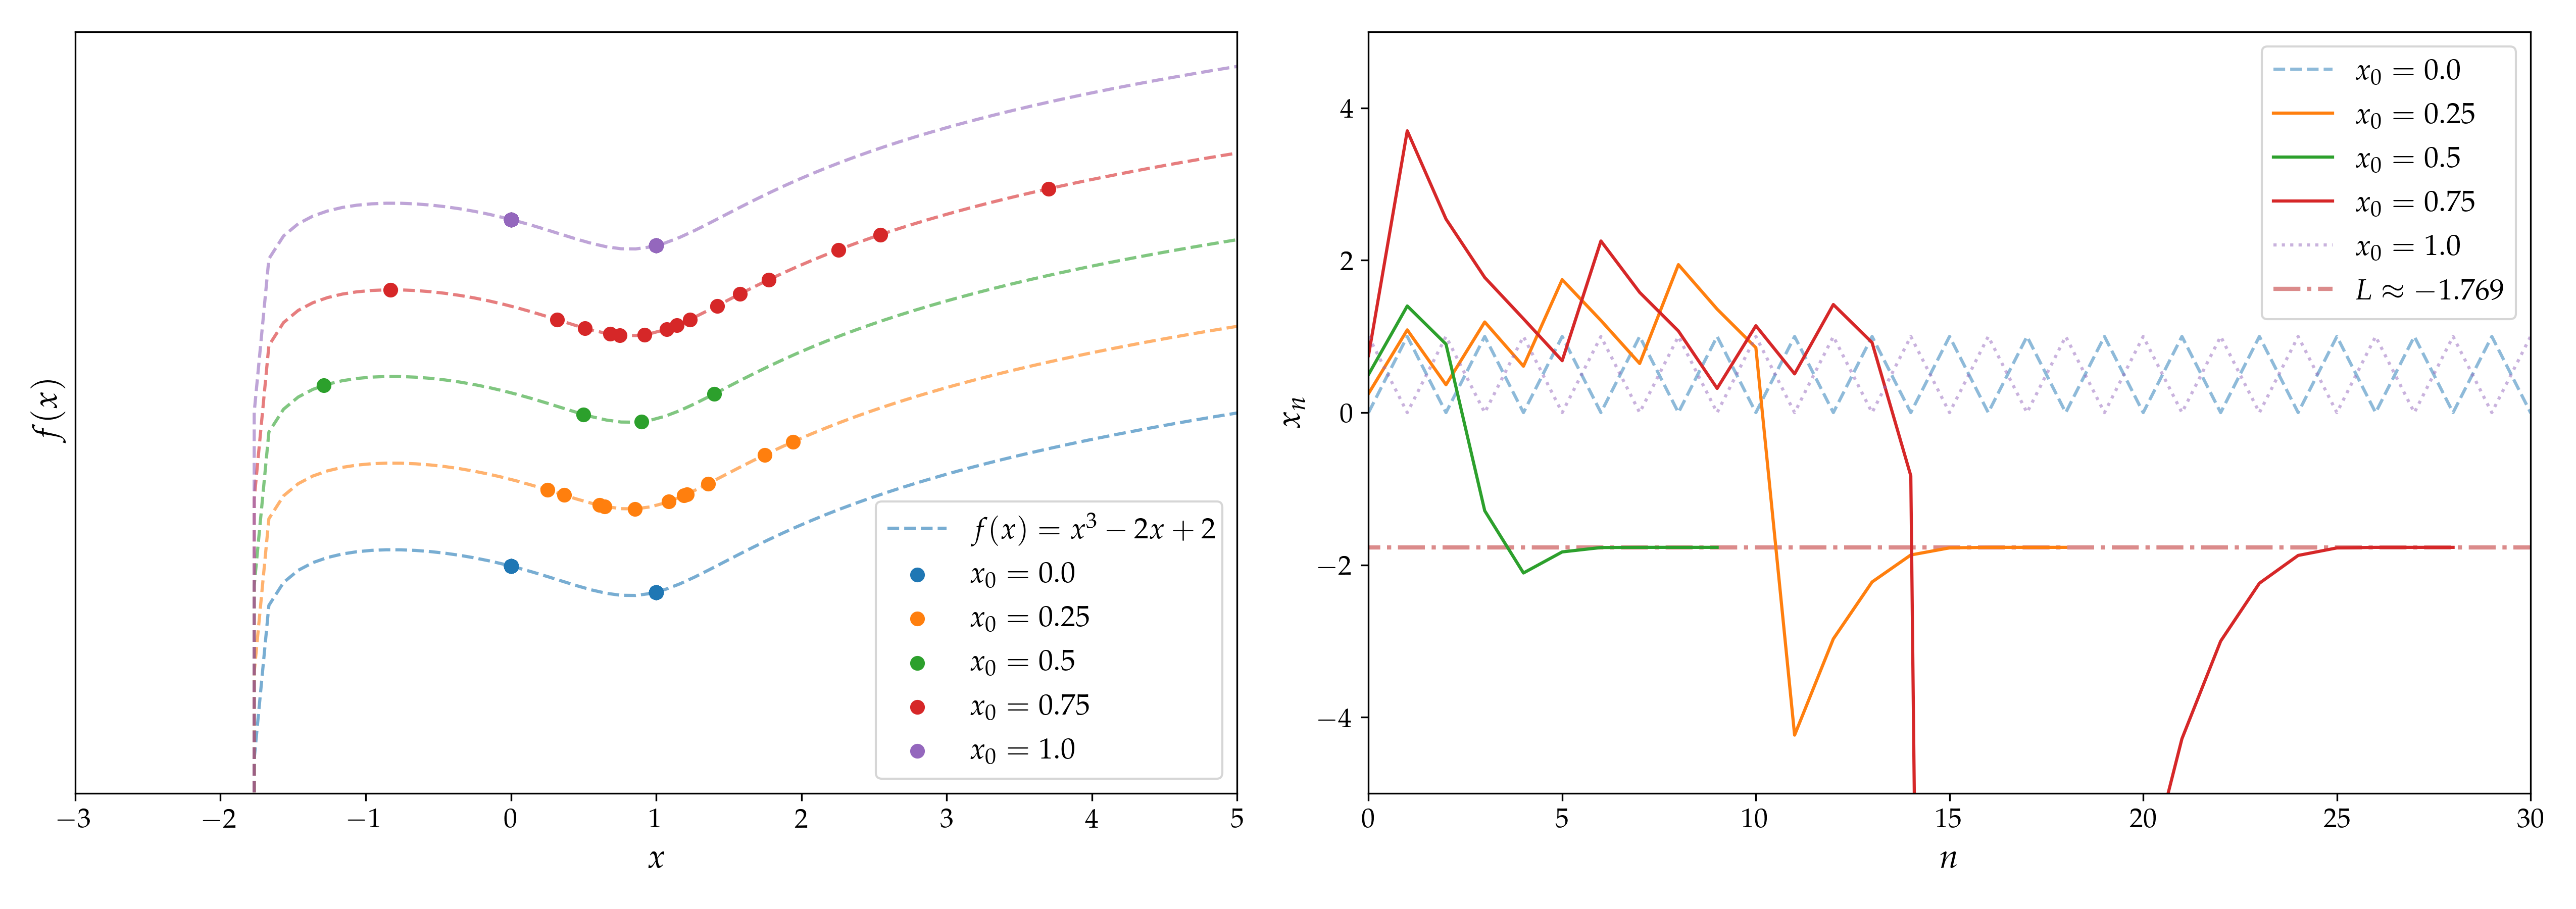
\includegraphics[width=0.9\linewidth]{images/13/fn_plot.png}
    \caption{La figura mostra a sinistra il plot di $f(x)$, con l'asse y con scala $\log_{10}$: è stato possibile moltiplicare per un fattore $n\cdot 10$ per spostare di $n$ unità in alto le linee e i punti, evitando la sovrapposizione. Ai diversi colori corrispondono diverse condizioni iniziali, con un range di $x_0 \in [0, 1]$.\\
    Nel grafico a destra si rappresenta la storia dell'algoritmo, per mostrare come procede la convergenza in funzione del numero di iterazioni: per tutti i punti intermedi è possibile terminare il programma con una stima di $L$, mentre nel caso di $x_0=0, 1$ si nota l'oscillazione indefinita tra i due valori.}
    \label{fig: NR conv 0,1}
\end{figure}

\begin{figure}[H]
    \centering
    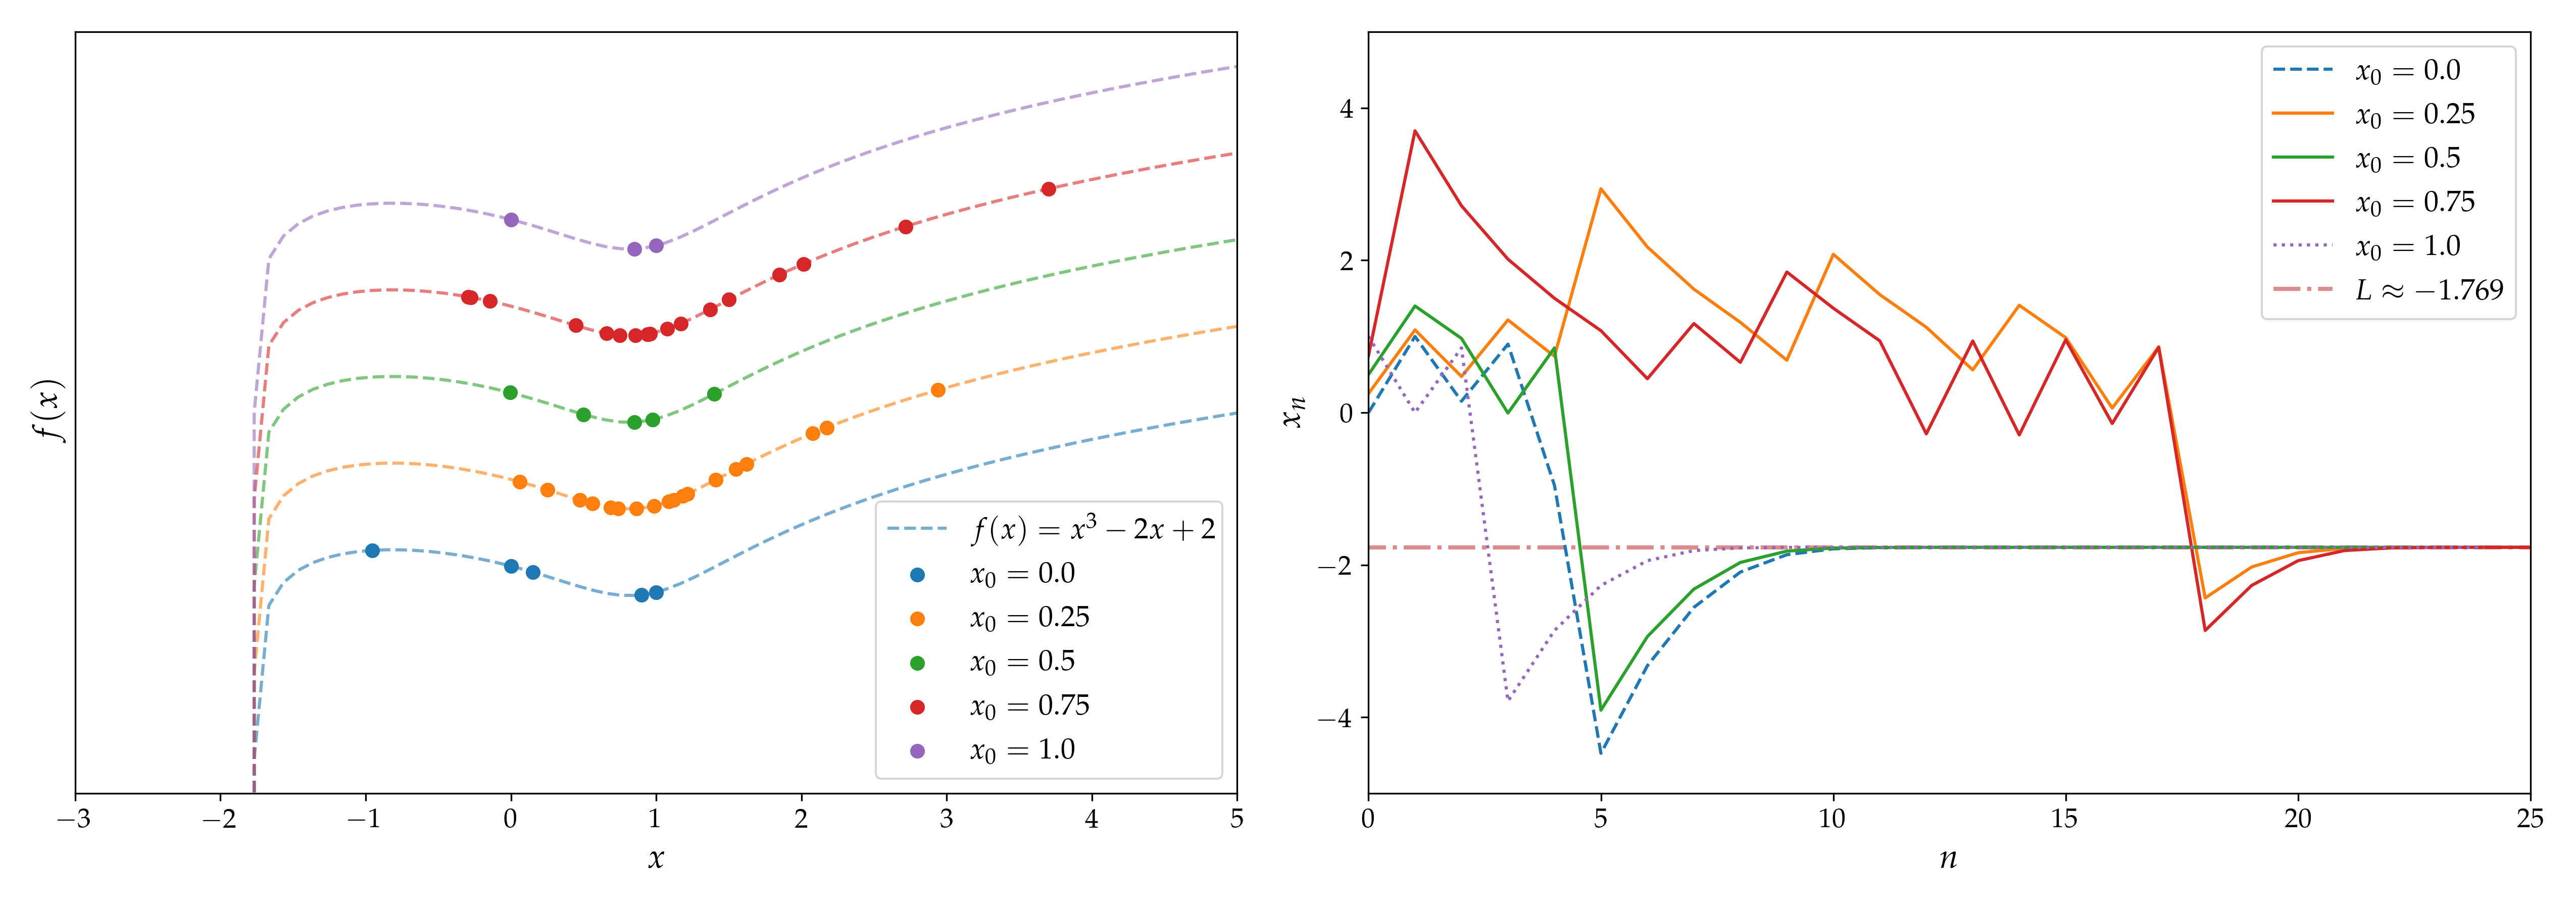
\includegraphics[width=0.9\linewidth]{images/13/fn_plot_correction.png}
    \caption{Figura analoga a Fig. \ref{fig: NR conv 0,1}, ma valutata usando l'algoritmo di Newton con la correzione introducendo il fattore $\lambda$. È possibile osservare come venga rotta la ciclicità che portava allo stagnamento e alla non convergenza che si osservavano nell'esempio precedente.}
    \label{fig: NR conv correction}
\end{figure}


\subsubsection{Condizioni iniziali}
L'ultimo esercizio propone di approfondire il problema delle condizioni iniziali, decidendo di scegliere diversi punti con cui inizializzare la ricerca dello zero e osservare come essa converga differentemente in funzione di questi.\\
In particolare si scelga la funzione
\[
f(x) = z^4 - 1, \quad z \in \mathbb{C}
\]
che ha come zeri $c = 1, -1, i -i$: restringendo il dominio di studio al quadrato sul piano complesso $Q=[-1, 1]\times[-1, 1]$, di seguito si mostrano i risultati dell'analisi. 

\medskip
\noindent In Fig. \ref{fig: fractal err mat} vediamo il controllo che è stato fatto sui risultati dell'algoritmo: si impone di ottenere un errore massimo tra la radice valutata numericamente e la più vicina delle 4 aspettate analiticamente, che sia minore di una certa soglia, impostata a $1e-9$. Formalmente:

\[
\forall z \in Q:\quad \sigma(z) = \min(|c_z - c|), \quad c \in \{1, -1, i, -i\}
\]

\noindent Imponendo che
\[
\max(\sigma) \le \varepsilon = 1e-9
\]

\bigskip\noindent
Ogni radice possiede un proprio bacino di attrazione, ossia l'insieme dei punti iniziali che convergono a quella soluzione sotto iterazione di Newton.\\
In Fig. \ref{fig: fractal} una chiara rappresentazione della figura che
rappresenta i bacini di attrazione delle quattro radici. 
La complessa geometria dei confini tra tali regioni è responsabile dell'elevata sensibilità alle condizioni iniziali: essa possiede una struttura frattale: ingrandendo queste regioni continuano a comparire dettagli complessi a scale sempre più piccole.\\

\noindent $\forall z\in Q$ viene inizializzato il metodo di N-R e della soluzione $c_z$ viene disegnato l'argomento $\theta = \arg(c_z)$ con una mappa di colore. 
Il valore di questa coordinata polare si trova nell'intervallo $[-\pi, \pi]$, ed è mostrato sulla scala di colori: il problema che si riscontra è che la scelta della libreria \textit{numpy} è di gestire gli angoli delle variabili \textit{complex} usando il branch cut lungo l'asse $\Re(z)<0$, cioè appunto l'intervallo di angoli $[-\pi, \pi]$: in questa maniera, le piccole deviazioni della posizione della radice sul piano si trasformano in notevoli differenze nel valore dell'argomento, in base che essa si trovi leggermente sopra o sotto l'asse reale (la rappresentazione del fenomeno è espressa in Fig. \ref{fig: wrong_fractal}).

\medskip
\noindent La scelta che ho fatto per risolvere questo problema è stata quella di usare una colormap ciclica, cioè che riportasse gli stessi colori sugli estremi della scala: in questo modo a $\arg(z)=\pm \pi$ viene associata effettivamente la stessa colorazione.

\begin{figure}[H]
    \centering
    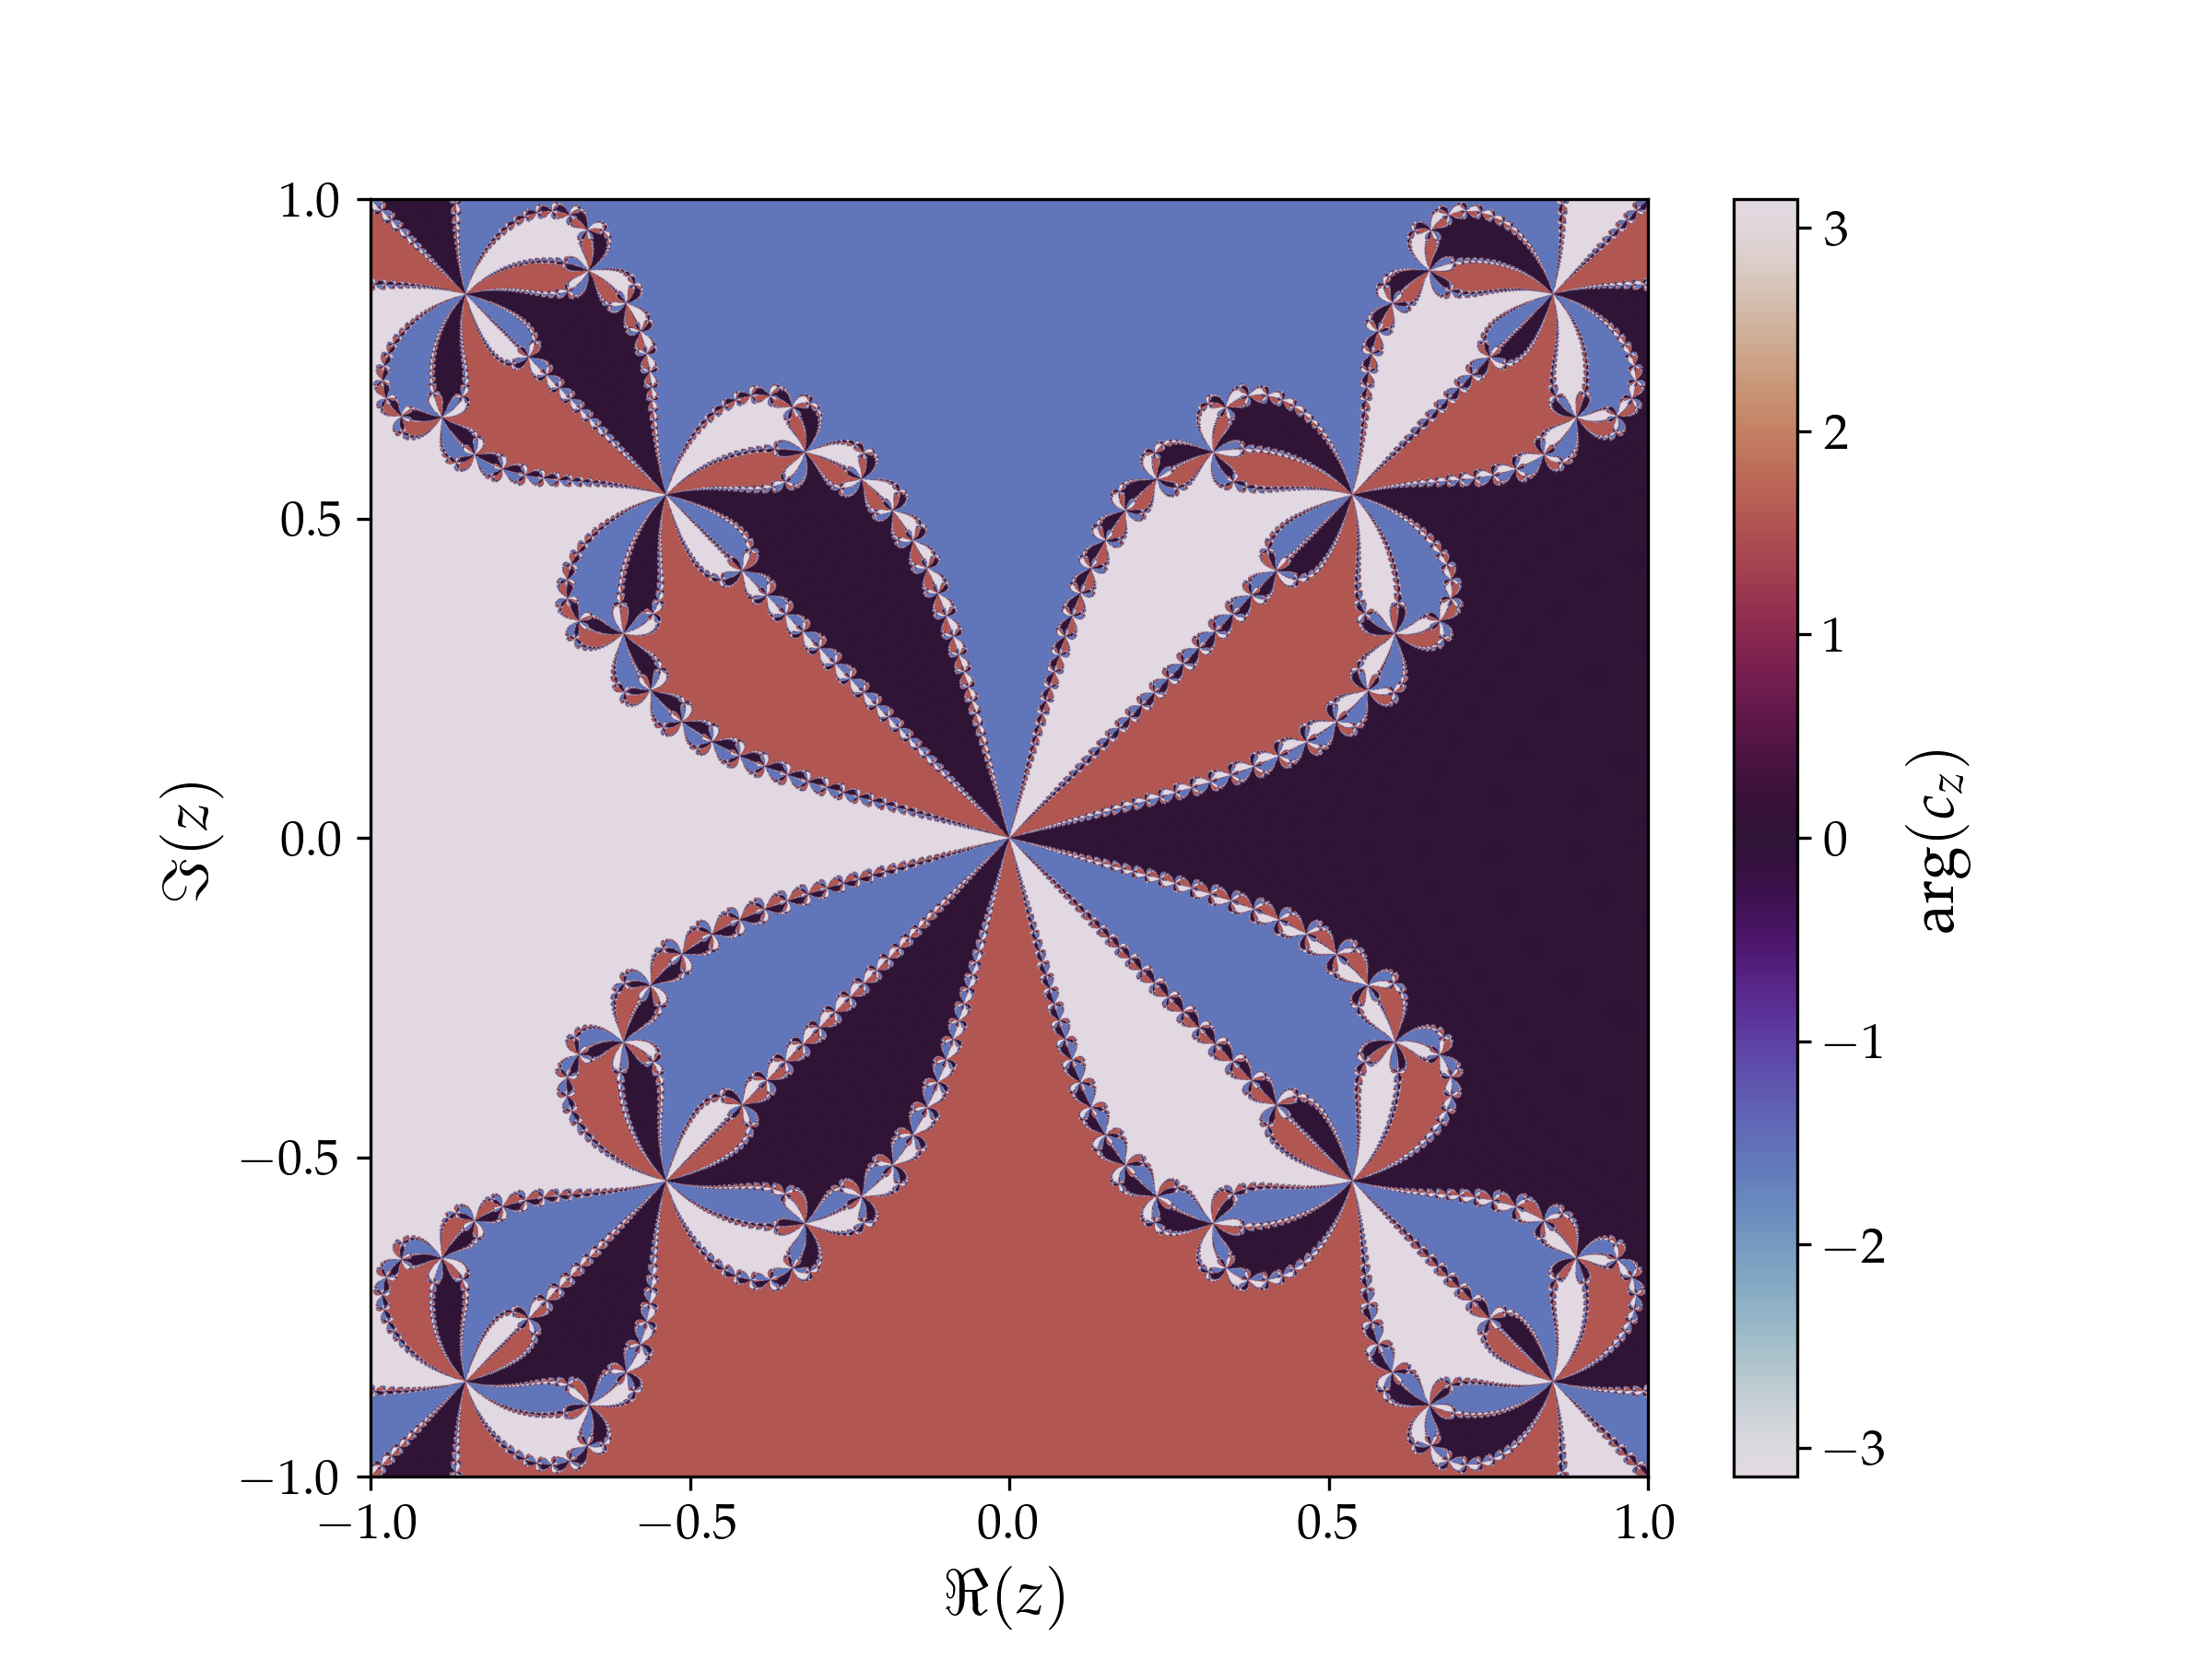
\includegraphics[width=0.75\linewidth]{images/13/fractal.png}
    \caption{La figura frattale che risulta dal plot dell'argomento della radice complessa che si ottiene impostando come $z_0$ un determinato punto $z$ del piano di Argand-Gauss. La scala di colori continua si riduce ad essere sostanzialmente discreta, poiché vengono selezionati solamente i quattro colori relativi alle soluzioni ($\theta = 0, \pm \pi, \pm\pi/2$).}
    \label{fig: fractal}
\end{figure}
\begin{figure}[H]
    \centering
    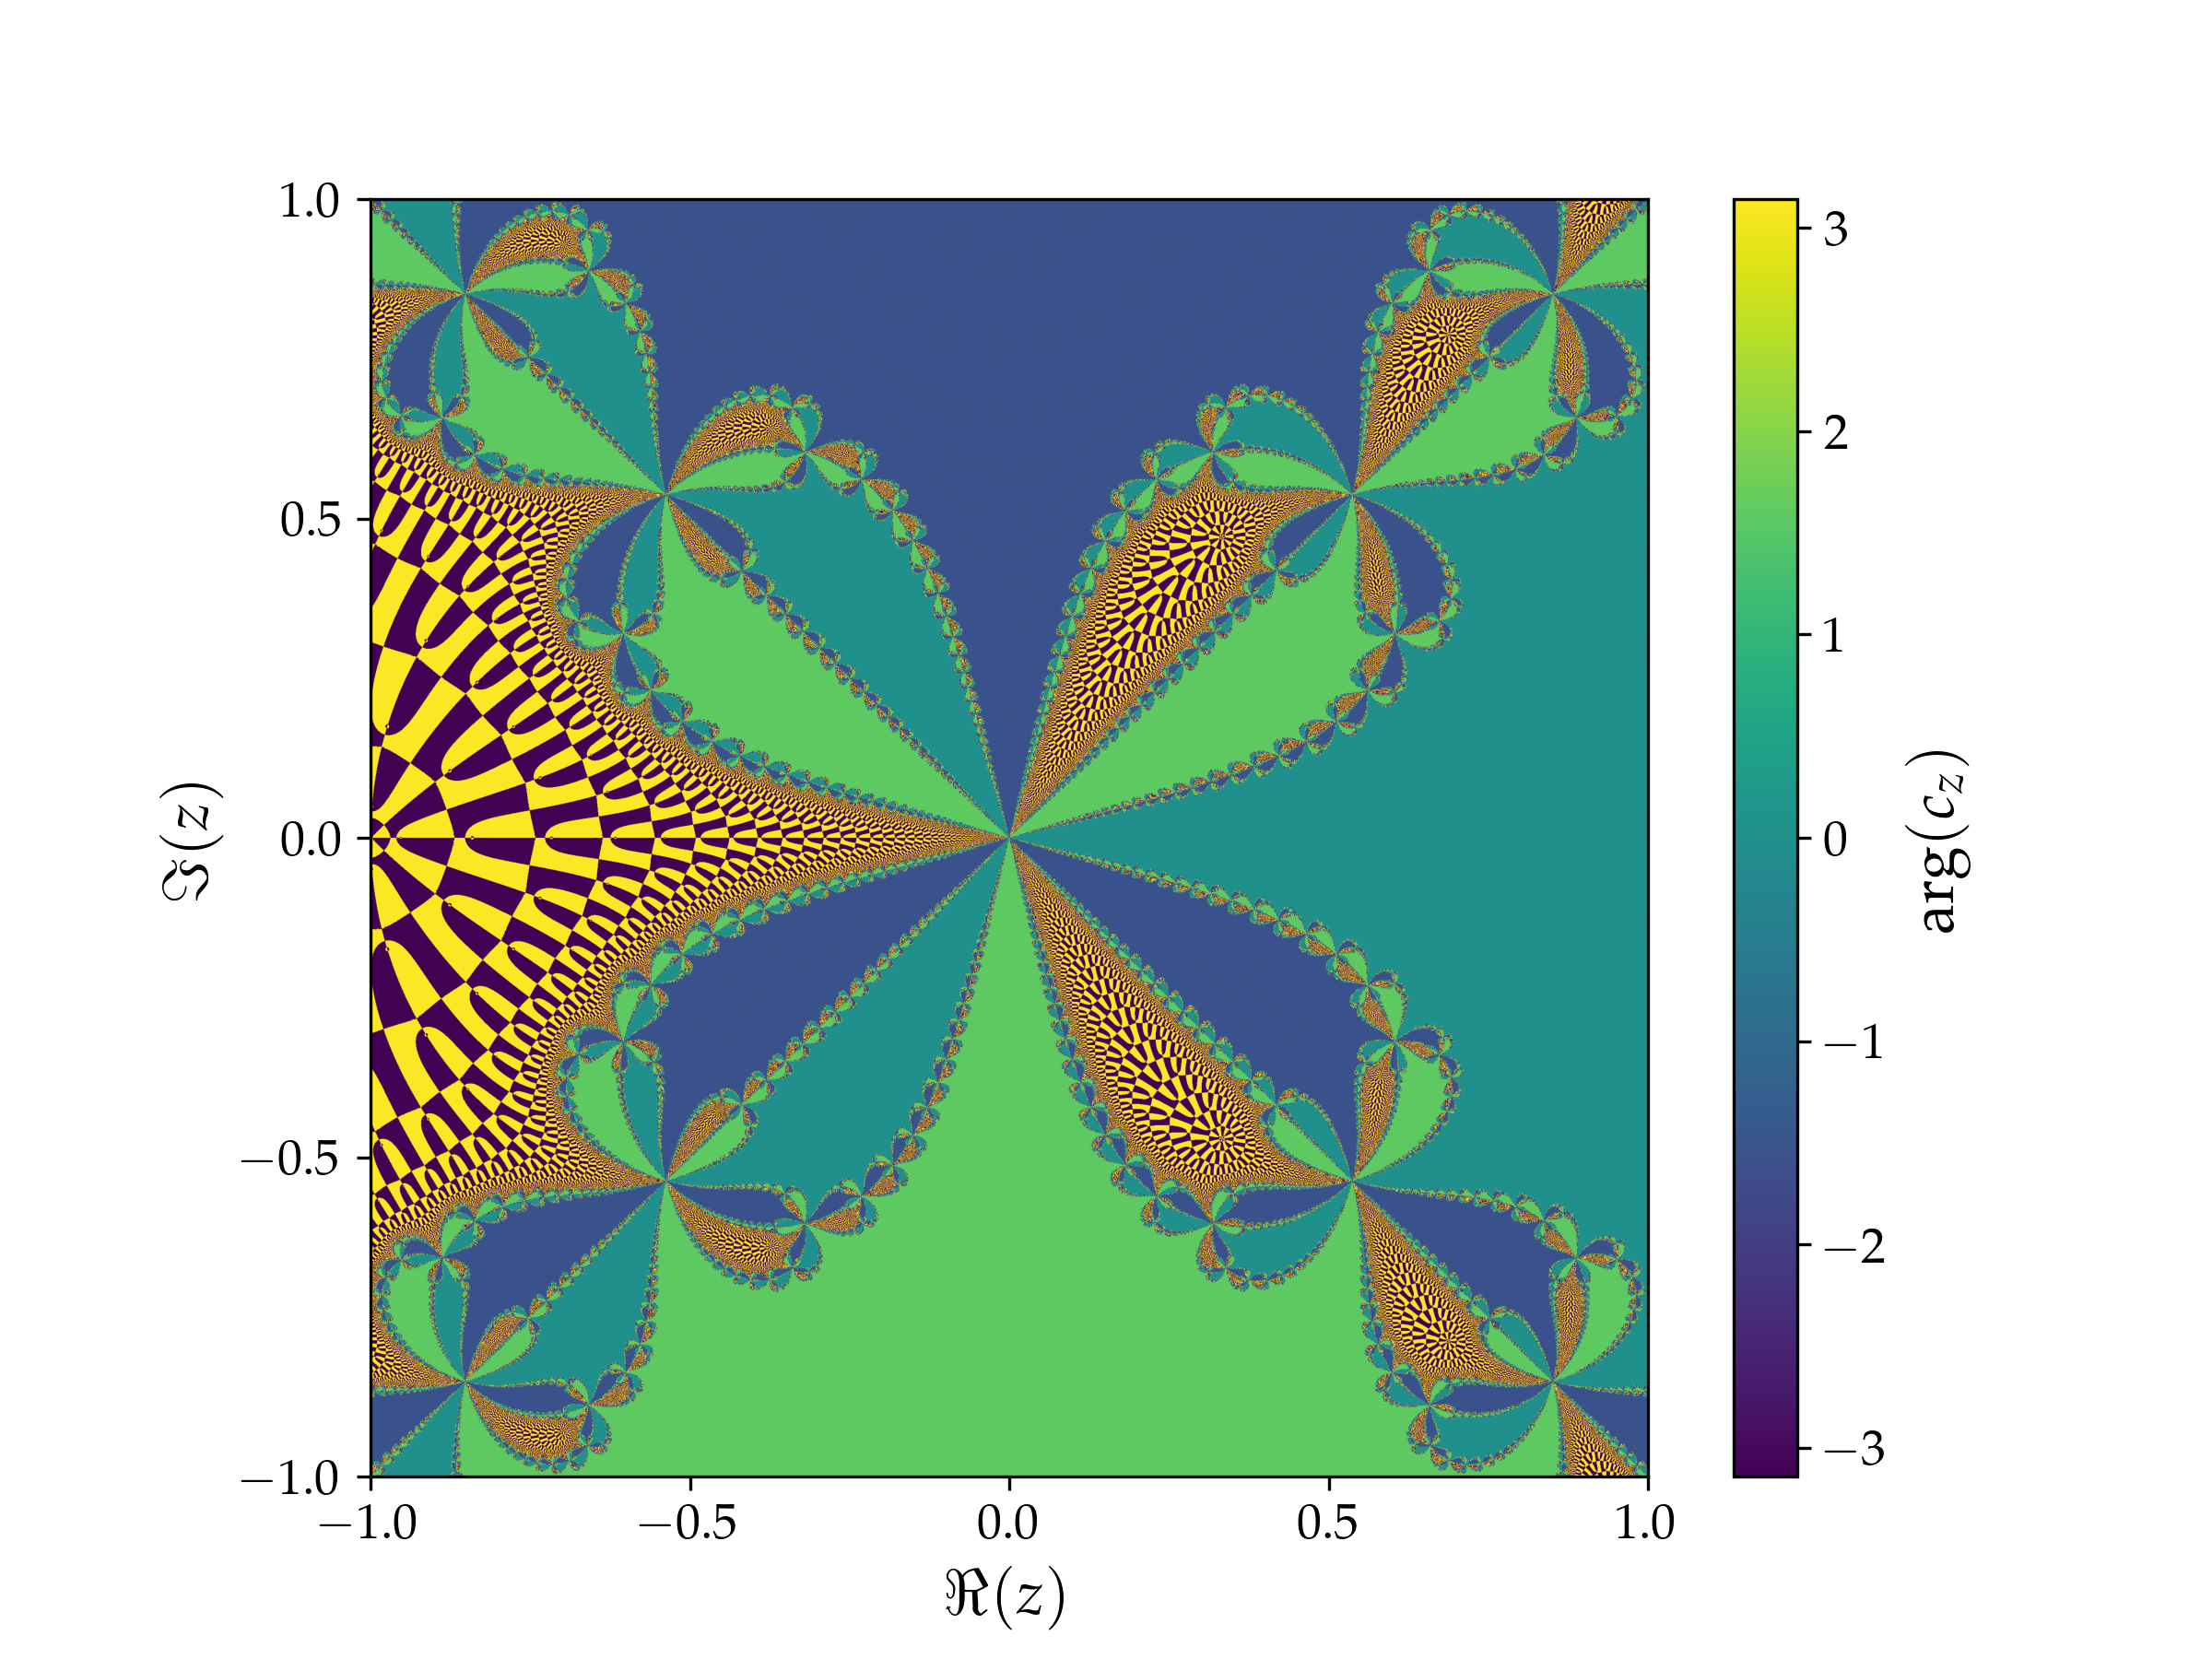
\includegraphics[width=0.75\linewidth]{images/13/wrong_fractal.png}
    \caption{La figura rappresenta, usando una colormap sequenziale come \textit{viridis}, che gli errori sulla ricerca della radice $-1$ comportano un certo grado di ambiguità sul valore dell'argomento di $c_z$.}
    \label{fig: wrong_fractal}
\end{figure}


\begin{figure}[H]
    \centering
    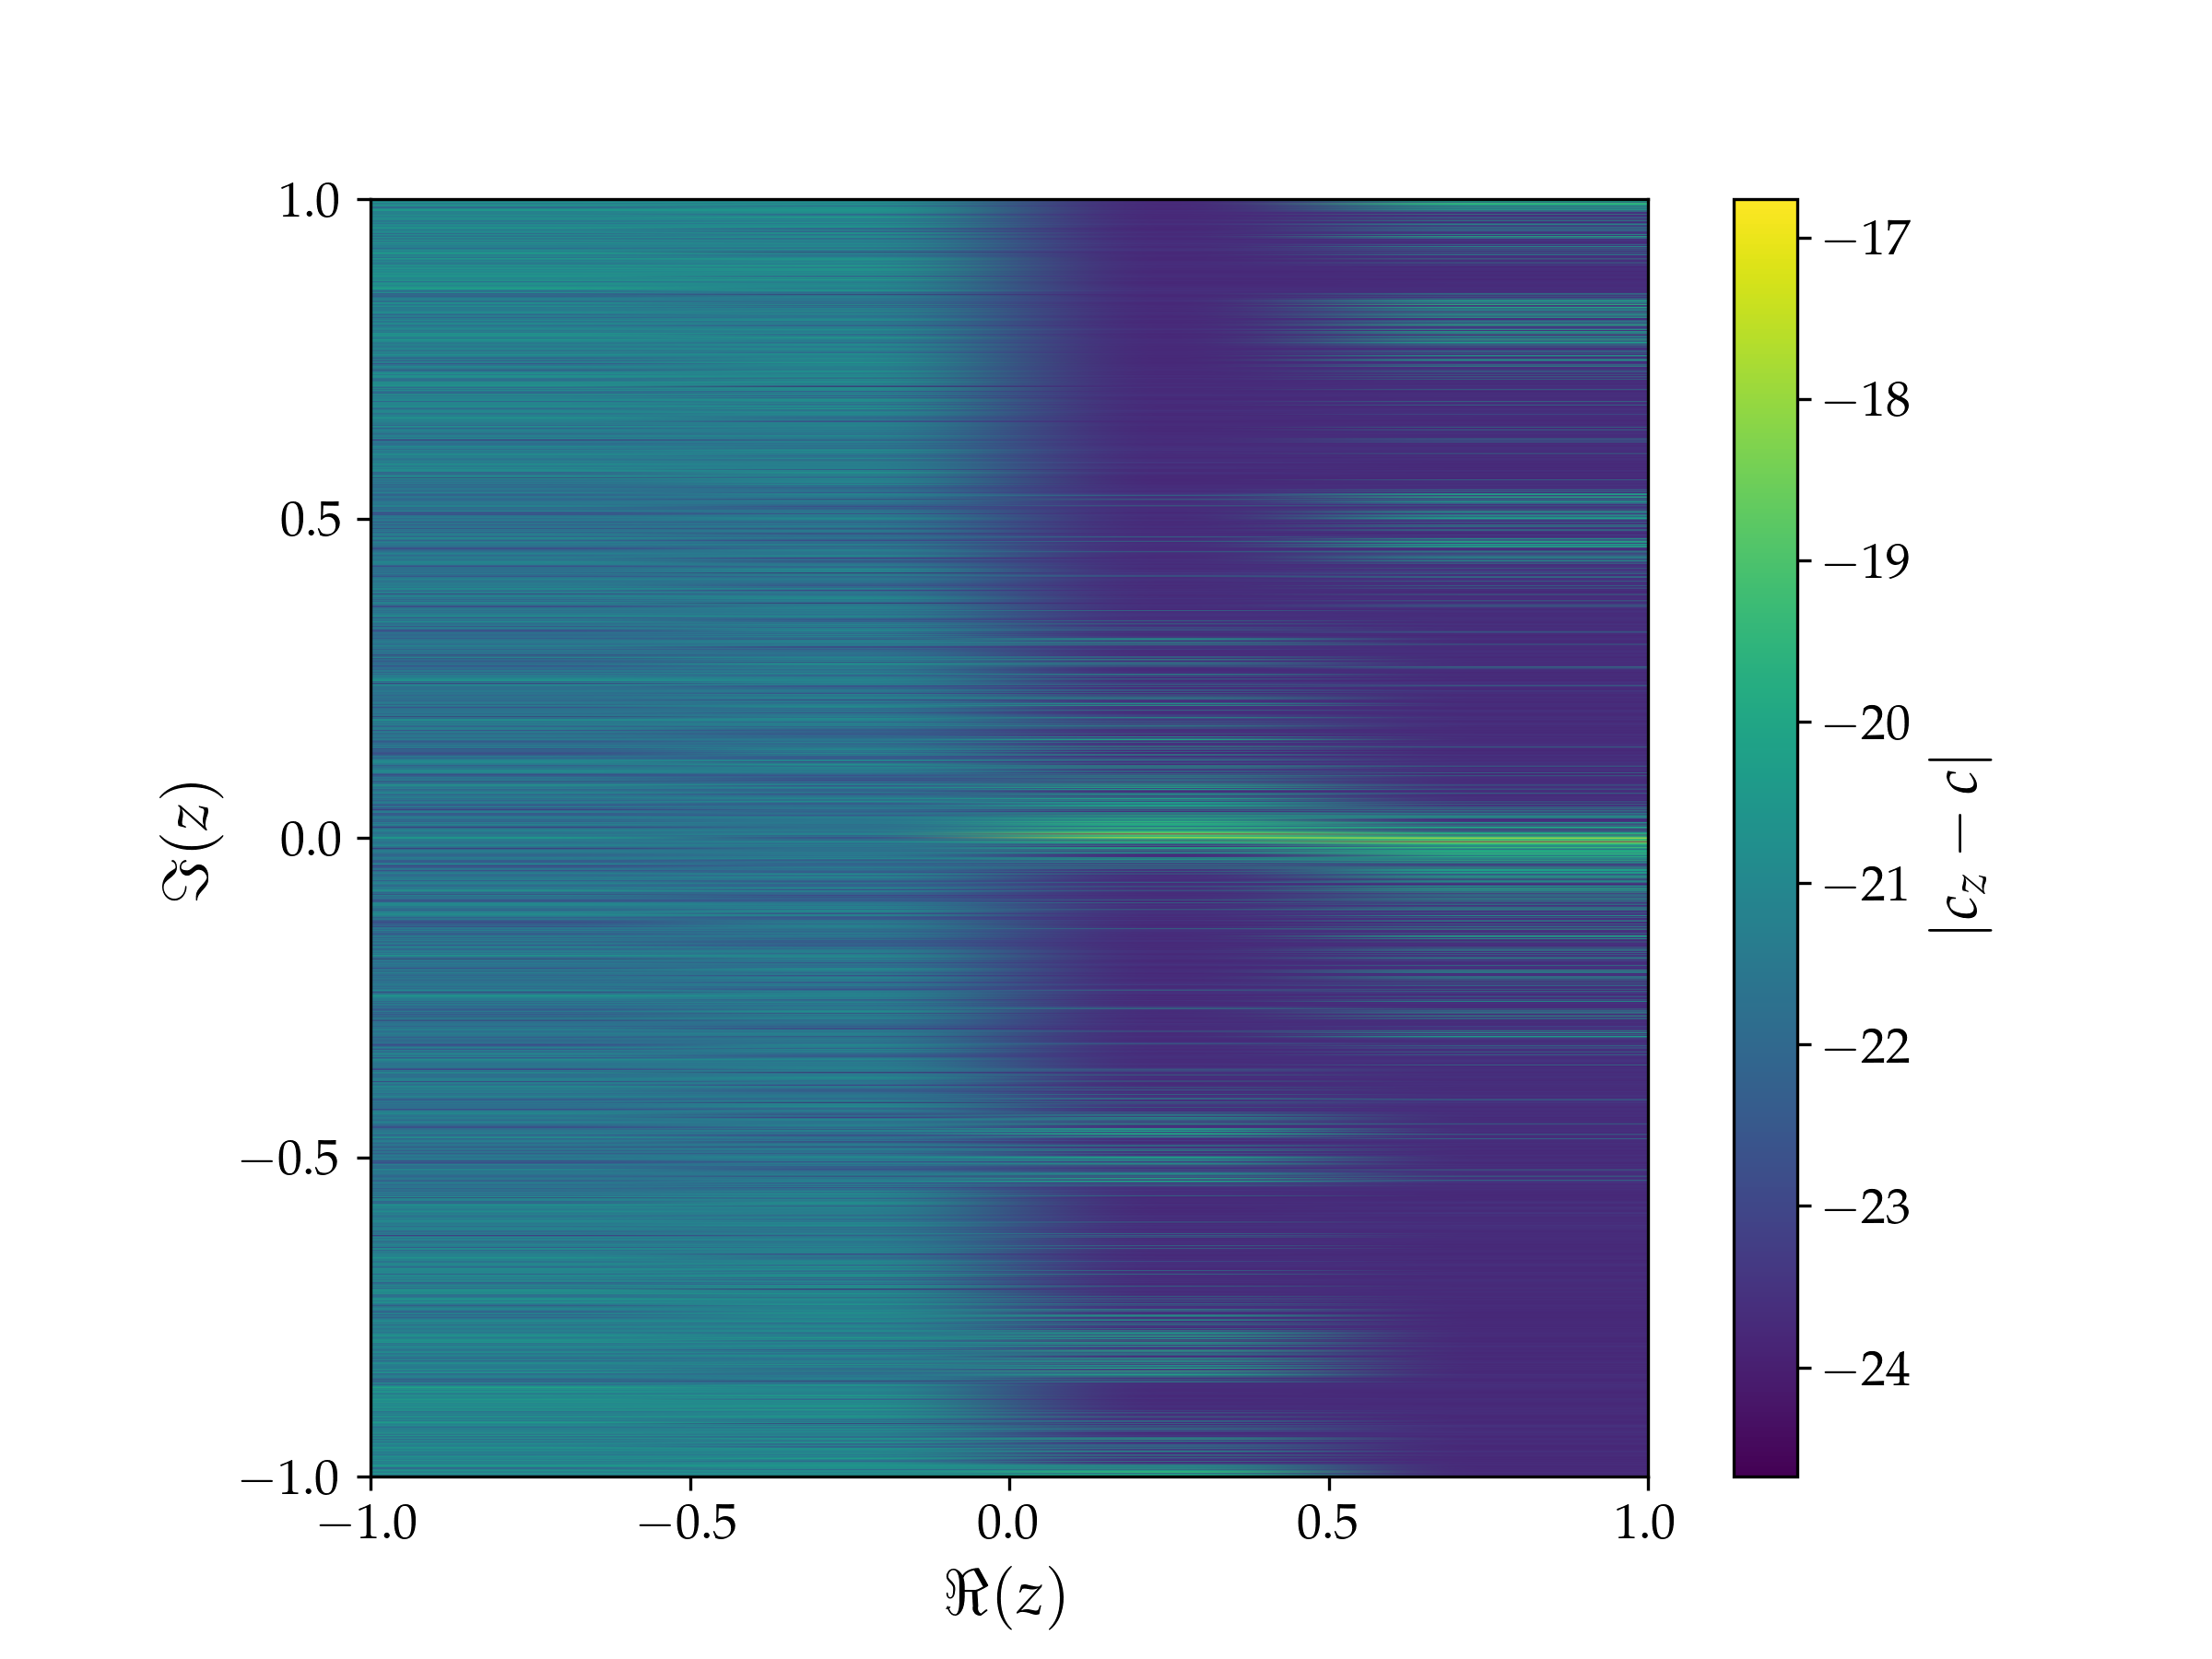
\includegraphics[width=0.8\linewidth]{images/13/error_matrix.png}
    \caption{Mappa della distanza (errore) rispetto alla radice più vicina: la scala logaritmica mostra che gli errori sono globalmente piccoli (è stato impostato un fondo scala di $1e-25$ per evitare possibili coincidenze $c_z=c$). Questo errore è ottenibile grazie ad una correzione che viene applicata sul metodo di Newton: per evitare la singolarità in $z=0$ ho introdotto una regolarizzazione numerica $f'(z+\epsilon)$, dove $\epsilon=1e-5$ è la più piccola deviazione che permette di avere un errore massimo sotto la tolleranza di $\text{Max err} \le 1e-9$. In questo esempio otteniamo $\text{Max err} = 1.73e-17<1e-9$.\\
    Questa modifica non fa parte del metodo di Newton standard ma è stata utilizzata esclusivamente per stabilizzare il calcolo sulla griglia discreta.}
    \label{fig: fractal err mat}
\end{figure}


\newpage












\section{Esercizio 5.2.3}
\subsection{Problem Statement}
Risolvi le equazioni trascendenti per $\hbar = 1, m = L = 1$ e $V_0 = 10$ utilizzando gli algoritmi di bisezione, Regula Falsi e Newton-Raphson/Secante. Sentiti libero di decidere se vuoi calcolare a mano le derivate prime o se invece vuoi utilizzare il metodo della Secante.

\vspace{1em}
\begin{enumerate}
    \item Trova la radice di $f_{\text{pari}}$ e confronta il tasso di convergenza dei tre metodi (studiando $|c - c_{\text{esatto}}|$ e $|f(c)|$ in funzione delle iterazioni in un unico grafico). Usa un intervallo ragionevole nella regione al di sotto di $-6$ per i metodi di bracketing e $x_0 < -6$ per quello di Newton.
    
    \item Dimostra che la convergenza è lineare per il metodo di bisezione e quadratica per il metodo di Newton partendo dai dati raccolti.
    
    \item Prova a scegliere diversi valori iniziali a destra della discontinuità per il metodo di Newton, nello specifico nell'intervallo $[-5.2, -5.0]$ e monitora, ovvero traccia un grafico, della soluzione per le prime 10-20 iterazioni. Cosa impari?
    
    \item Traccia il grafico dell'equazione trascendente dispari per individuare approssimativamente le altre radici. Quindi passa un intervallo di input ragionevole ai metodi di bracketing e un'ipotesi di partenza ragionevole per l'algoritmo di Newton.
\end{enumerate}

\subsection{Premessa Teorica}
Per una massa $m$ le funzioni d'onda nella buca di potenziale finita ($-\infty <V_0<+\infty$) 1-dimensionale sono descritte da delle equazioni trascendenti, non risolvibili analiticamente, ma che richiedono una soluzione numerica. Lo spettro dei livelli energetici è discreto e definito da $E$: questa configurazione è detta di \textit{stato legato}.\\
Per gli stati pari vale la seguente equazione:
\[
k(E) \tan\left(\frac{k(E) L}{2}\right) = \bar\kappa(E)
\]

mentre per quelli dispari:
\[
k(E) \cot\left(\frac{k(E) L}{2}\right) = -\bar\kappa(E)
\]

considerando
\[
k(E) = \sqrt{\frac{2 m (V_0 + E)}{\hbar^2}}, \quad
\bar\kappa(E) = \sqrt{\frac{-2 m E}{\hbar^2}}
\]

\medskip\noindent
Per la risoluzione in funzione di $E$, cioè la ricerca del livello energetico, fissate le condizioni al contorno, è possibile ridefinire l'analisi come la ricerca di uno zero di $f(E)$ così definita:
\begin{align*}
f_\mathrm{pari}(E) &= k(E) \tan\left(\frac{k(E) L}{2}\right) - \bar\kappa(E)\\
f_\mathrm{dispari}(E) &= k(E) \cot\left(\frac{k(E) L}{2}\right) + \bar\kappa(E)
\end{align*}

\subsection{Metodi Numerici e Algoritmi}
Decidiamo di introdurre un nuovo algoritmo, per la ricerca degli zeri di una funzione, rivedendo la definizione del N-R, ma combinandolo con queste caratteristiche:
\begin{itemize}
    \item Evitare il calcolo analitico della derivata, che può, in alcuni casi, essere complesso o dispendioso.
    \item Avere un rate di convergenza maggiore rispetto a quello lineare della bisezione o Regula Falsi.
    \item Massimizzare l'efficienza computazionale, ottimizzando al massimo le valutazioni della funzione, soprattutto in caso che essa sia molto complessa e computazionalmente pesante.
\end{itemize}

Nasce così il \textit{Metodo delle Secanti}, che rispecchia proprio queste tre caratteristiche.
Partendo dal ben conosciuto algoritmo di Newton-Raphson, possiamo decidere di ridefinire la derivata prima, non come funziona analitica, ma usando le derivate finite, in particolare la definizione \textit{backward}:
\begin{align*}
\frac{f(x) - f(x-\epsilon)}{\epsilon} & = f'(x) + O(\epsilon) \\
\end{align*}
se $\epsilon$ è piccolo e rappresenta il passo dell'iterazione ($x_n - x_{n-1} = \epsilon$) il metodo N-R viene riscritto così:
\[
    x_{n+1} = x_n - f(x_n) \frac{x_n- x_{n-1}}{f(x_n) - f(x_{n-1})}
\]

Il rate di convergenza non è lineare né quadratico, ma è una via di mezzo fra questi: il metodo viene detto superlineare, poiché $1<p<2$, $p=\phi \approx1.618$. Inoltre si può osservare che mantendo in memoria $f(x_{n-1})$ dell'iterazione precedente, possiamo fare un'unica valutazione della funzione per iterazione. Questa definizione del punto $x_{n+1}$ come funzione di $x_n, x_{n-1}$ implica che l'algoritmo necessita di essere inizializzato con due punti, e non più solo uno come nel caso di N-R.

\subsection{Risultati e Discussione}
In primis si mostra un plot (Fig. \ref{fig: f even}) della funzione e della sua derivata nell'intervallo di interesse: si noti la presenza di una singolarità (asintoto verticale), che può compromettere la convergenza di Newton-Raphson e del metodo delle Secanti se l'inizializzazione cade troppo vicino alla discontinuità o conduce l'iterazione ad attraversarla.

\begin{figure}[H]
    \centering
    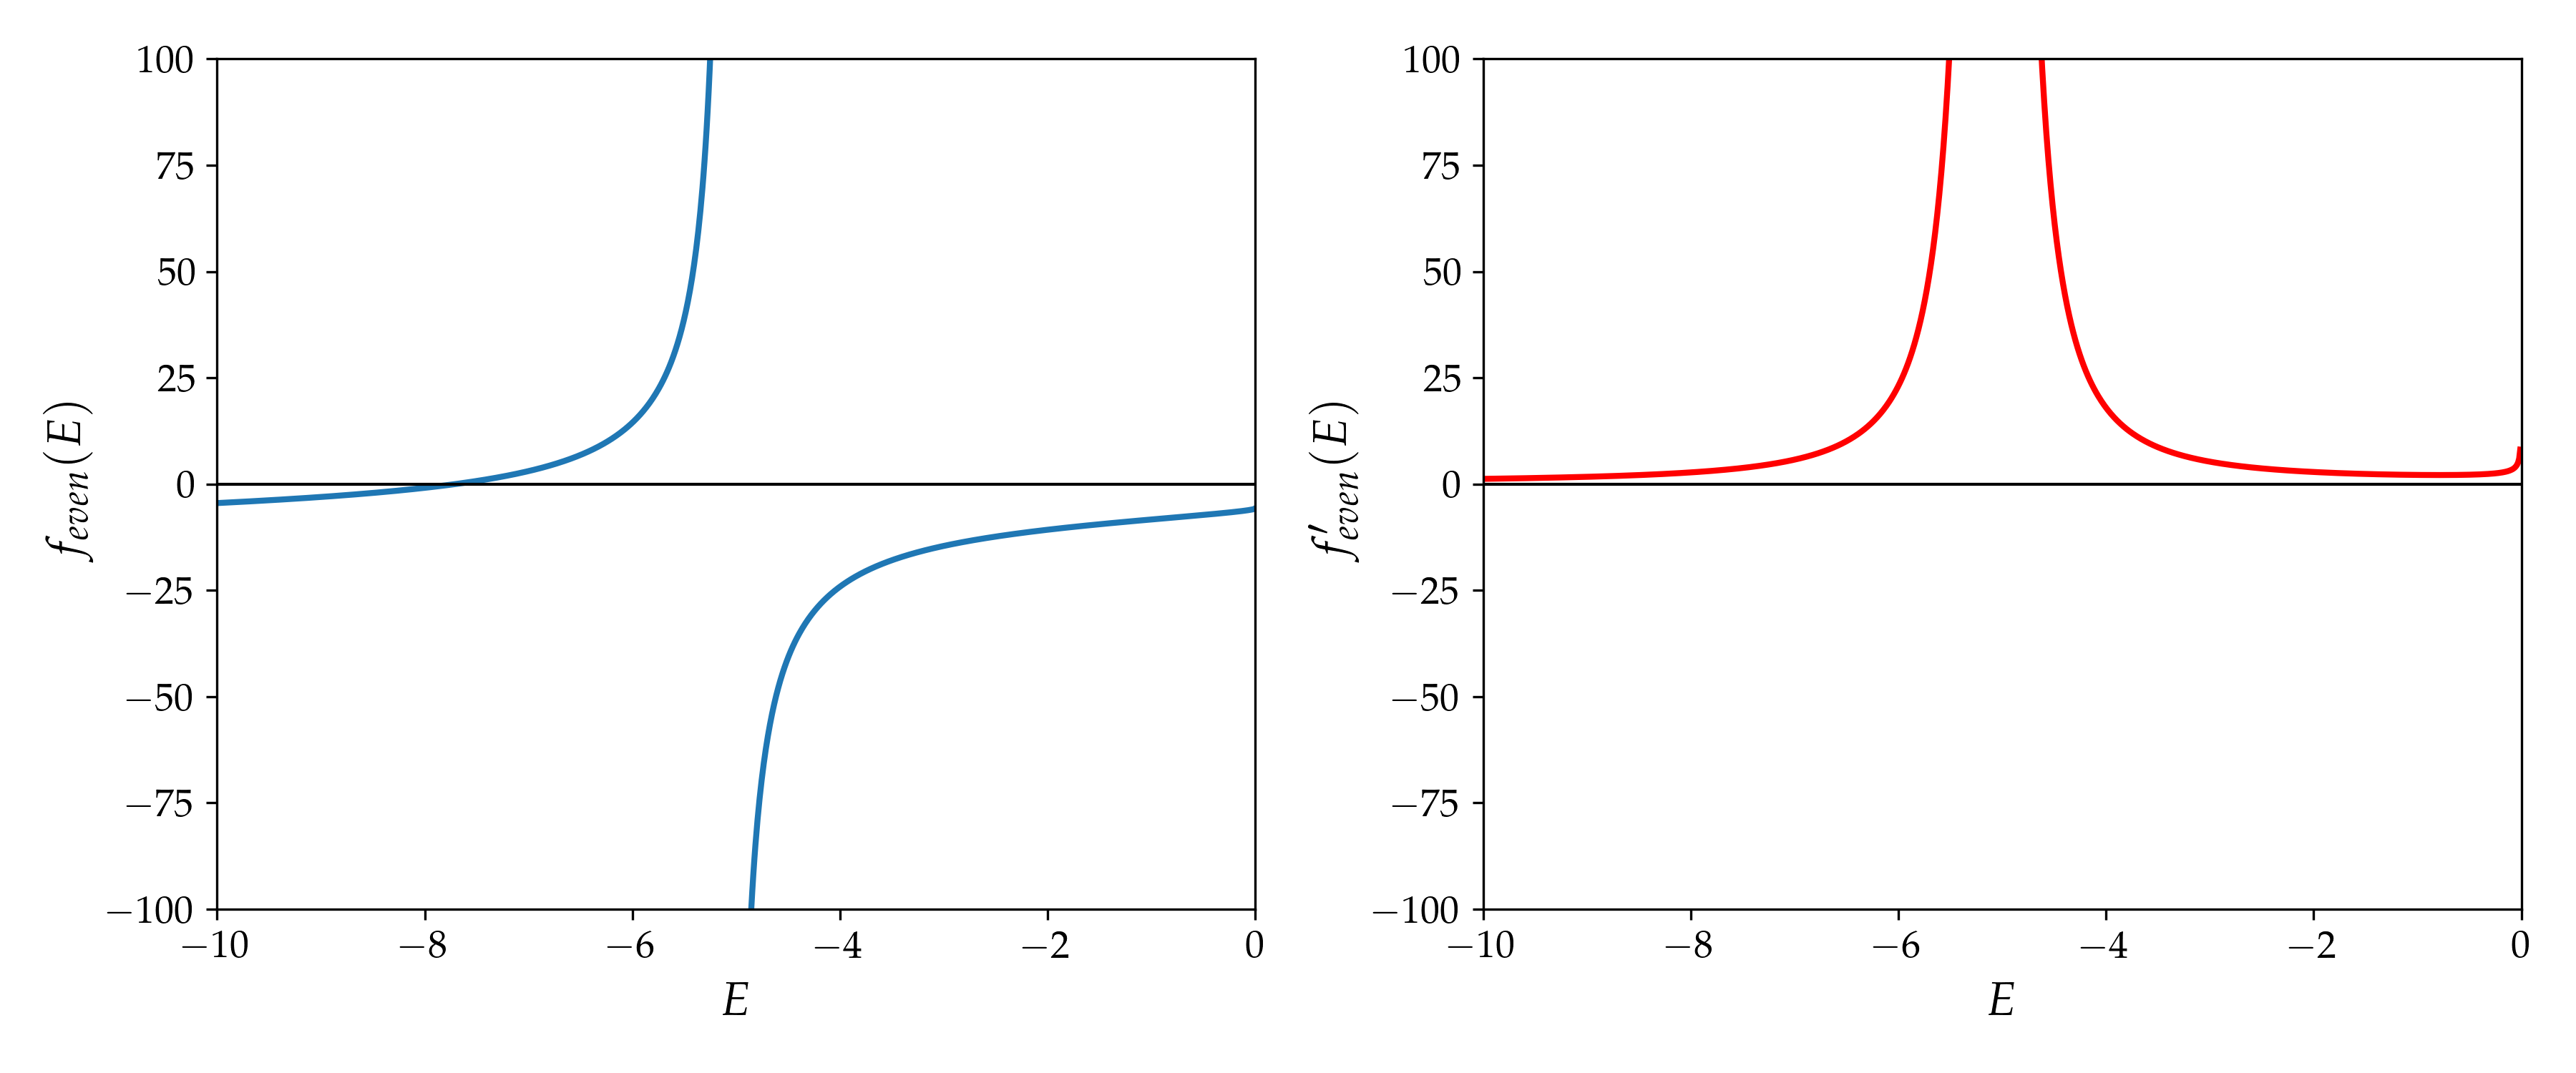
\includegraphics[width=\linewidth]{images/14/f_even.png}
    \caption{Plot della funzione pari e della sua derivata: si nota un punto di discontinuità.}
    \label{fig: f even}
\end{figure}

Vengono quindi comparati i quattro metodi presentati sino ad ora: ne studiamo la storia della radice e del valore della funzione, in termini del numero di iterazioni. Infine compariamo le convergenze e verifichiamo che si riscontrino i comportamenti aspettati.

\begin{elegantcode}[title={Risultati per i diversi algoritmi di ricerca}]
Bisection        c = -7.7050092507390815
                 iters = 47

Regula Falsi     c = -7.705009250739083
                 iters = 24

Secant           c = -7.7050092507390815
                 iters = 9

Newton-Raphson   c = -7.7050092507390815
                 iters = 8
\end{elegantcode}

È in Fig. \ref{fig: conv_even} che osserviamo una prima stima dei diversi comportamenti delle funzioni: qualitativamente è possibile vedere come Bisezione e Regula Falsi convergano in maniera lineare, mentre gli altri con una traiettoria più "parabolica", infine si nota che tra i due superlineari è Newton-Raphson ad avere la meglio e convergere più rapidamente.

\medskip\noindent
L'andamento vero e proprio delle funzioni, nella scala adatta, è fatto nei plot Fig. \ref{fig: confr even}, Fig. \ref{fig: even mean} e nei fit di Figs. \ref{fig: bisezione_fit}-\ref{fig: NR_fit} (per cui è sottinteso per ognuna l'approssimazione sull'intestazione degli assi di Fig.\ref{fig: fit Bis}.). È omessa l'incertezza legata alla stima del parametro di scaling per le considerazioni fatte, e già proposte, nell'appendice, perció non è possibile proporre i risultati del test del t-Student, poiché non attendibili come valutazioni statistiche: in particolare in Fig. \ref{fig: even mean} il valore stimato è la media aritmetica delle ascisse dei punti, statistica non rigorosa poiché i punti $e_{k+1}/e_k$ sono chiaramente non i.i.d. (indipendenti e identicamente distribuiti); per le figure riferite ai fit delle singole distribuzioni, il parametro è frutto della stima del fit con regressione lineare, ma anche in questo caso l'incertezza non è fornita, poiché viene usata la matrice di identità come covarianza (vedi Appendice).\\


\begin{figure}[H]
    \centering
    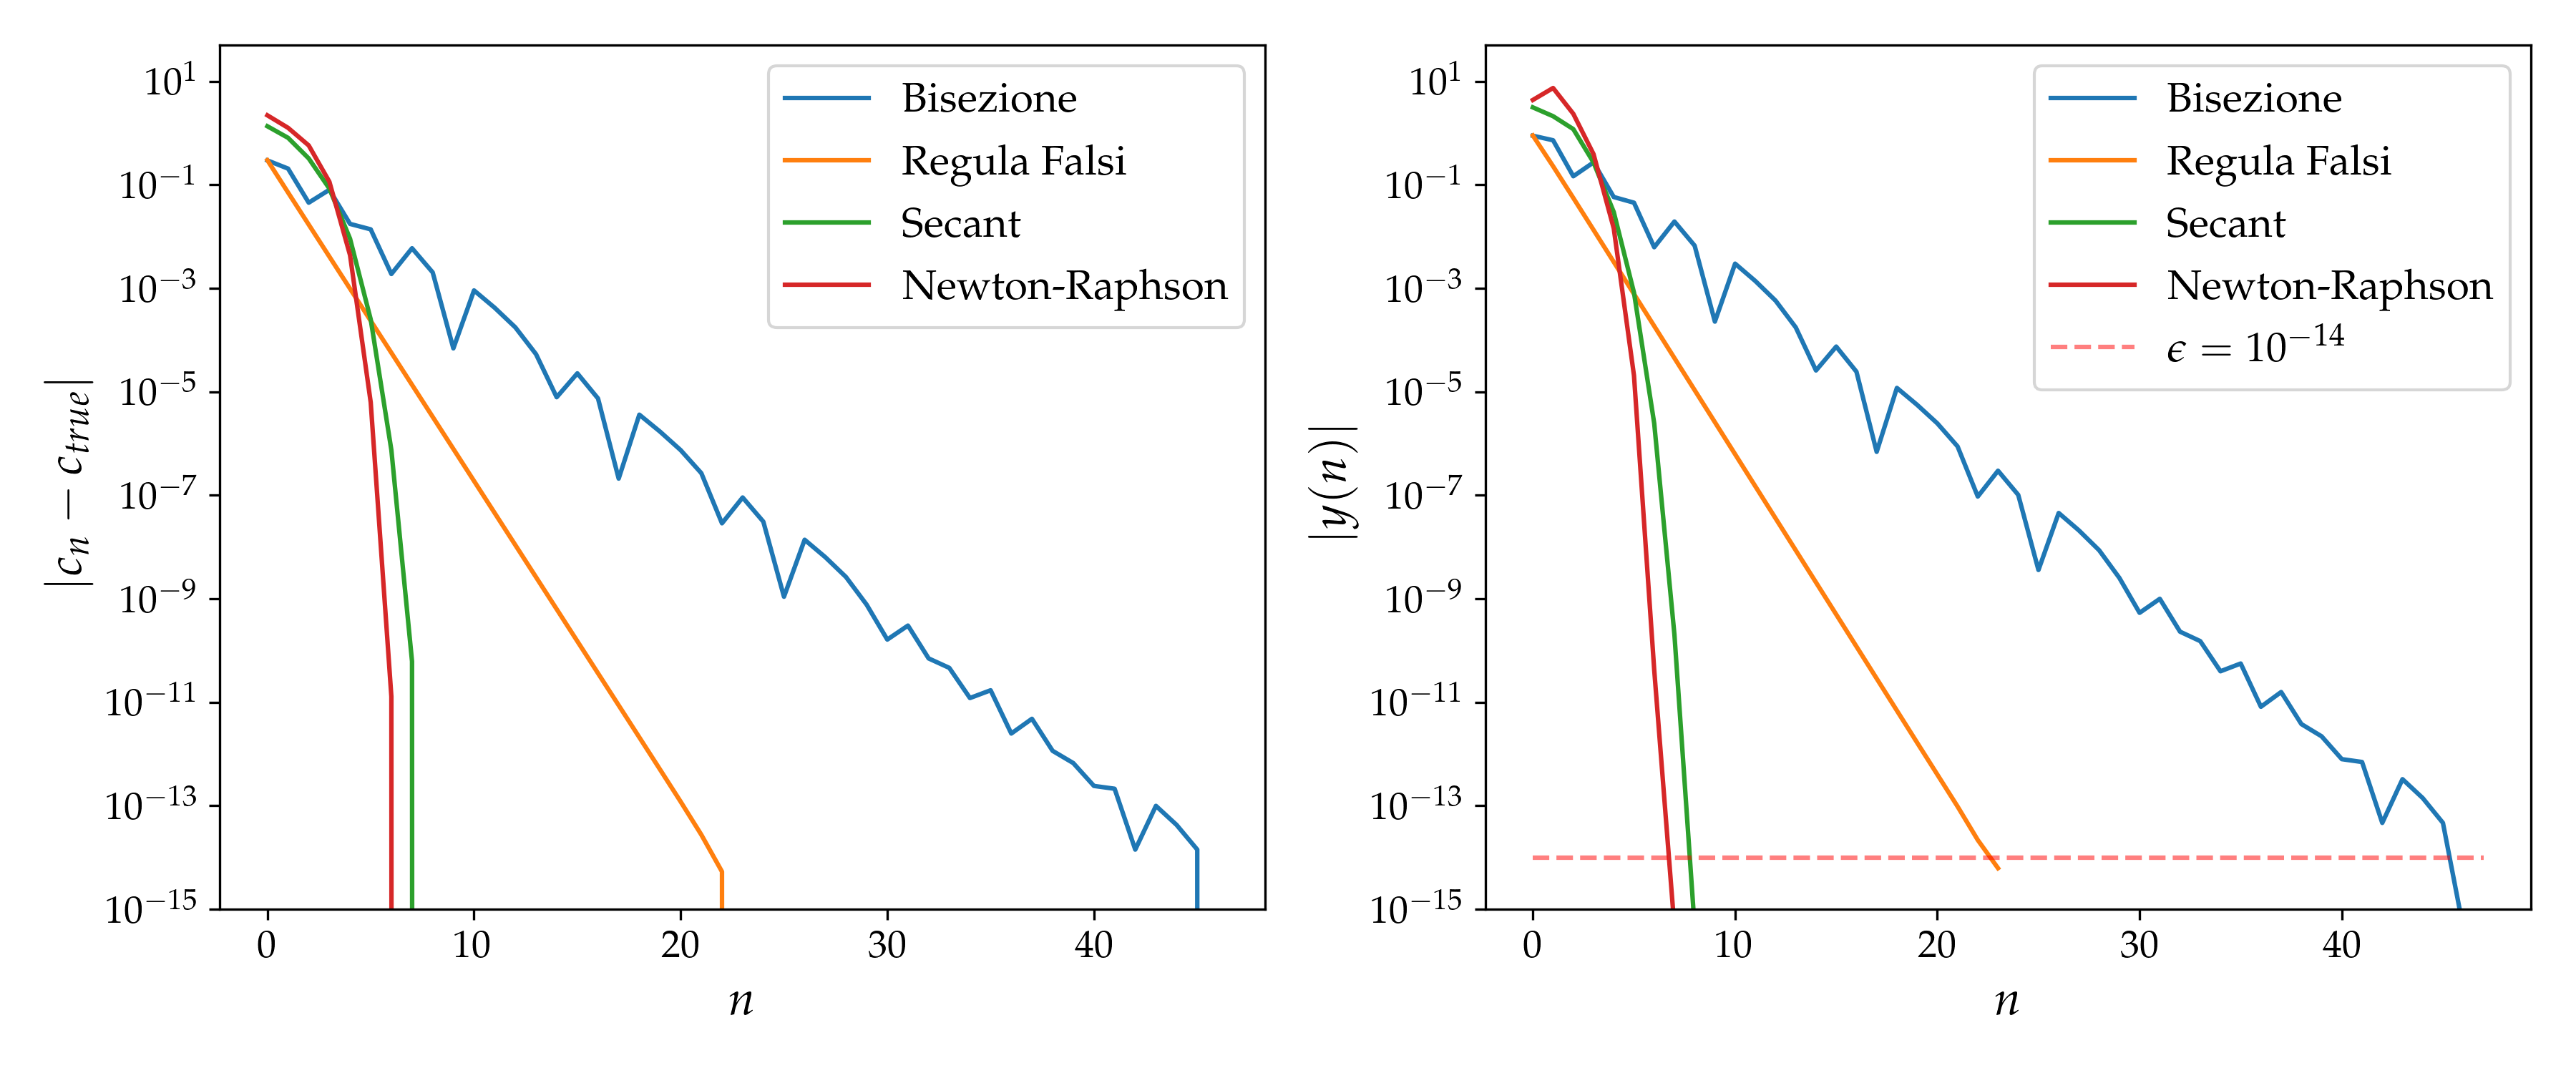
\includegraphics[width=\linewidth]{images/14/even_conv.png}
    \caption{Sulla sinistra il plot dell'errore rispetto alla radice vera (valutata come l'ultimo punto della successione, quando l'algoritmo converge e si ferma). A destra l'errore sulla funzione al passo n-esimo; sapendo che la funzione nella radice vale per definizione zero, si riduce ad essere il valore assoluto della funzione valutata nel punto $c_n$. Si noti come in questa seconda figura è anche indicata la tolleranza che è stata stabilita condivisa per tutti gli algoritmi: per definizione il metodo converge quando il valore della funzione nella \textit{guess} è minore di $\epsilon$, quindi vediamo che tutte le storie dei diversi algoritmi arrivano a convergenza e si fermano, solamente dopo aver superato questa soglia.}
    \label{fig: conv_even}
\end{figure}


\begin{figure}[H]
    \centering
    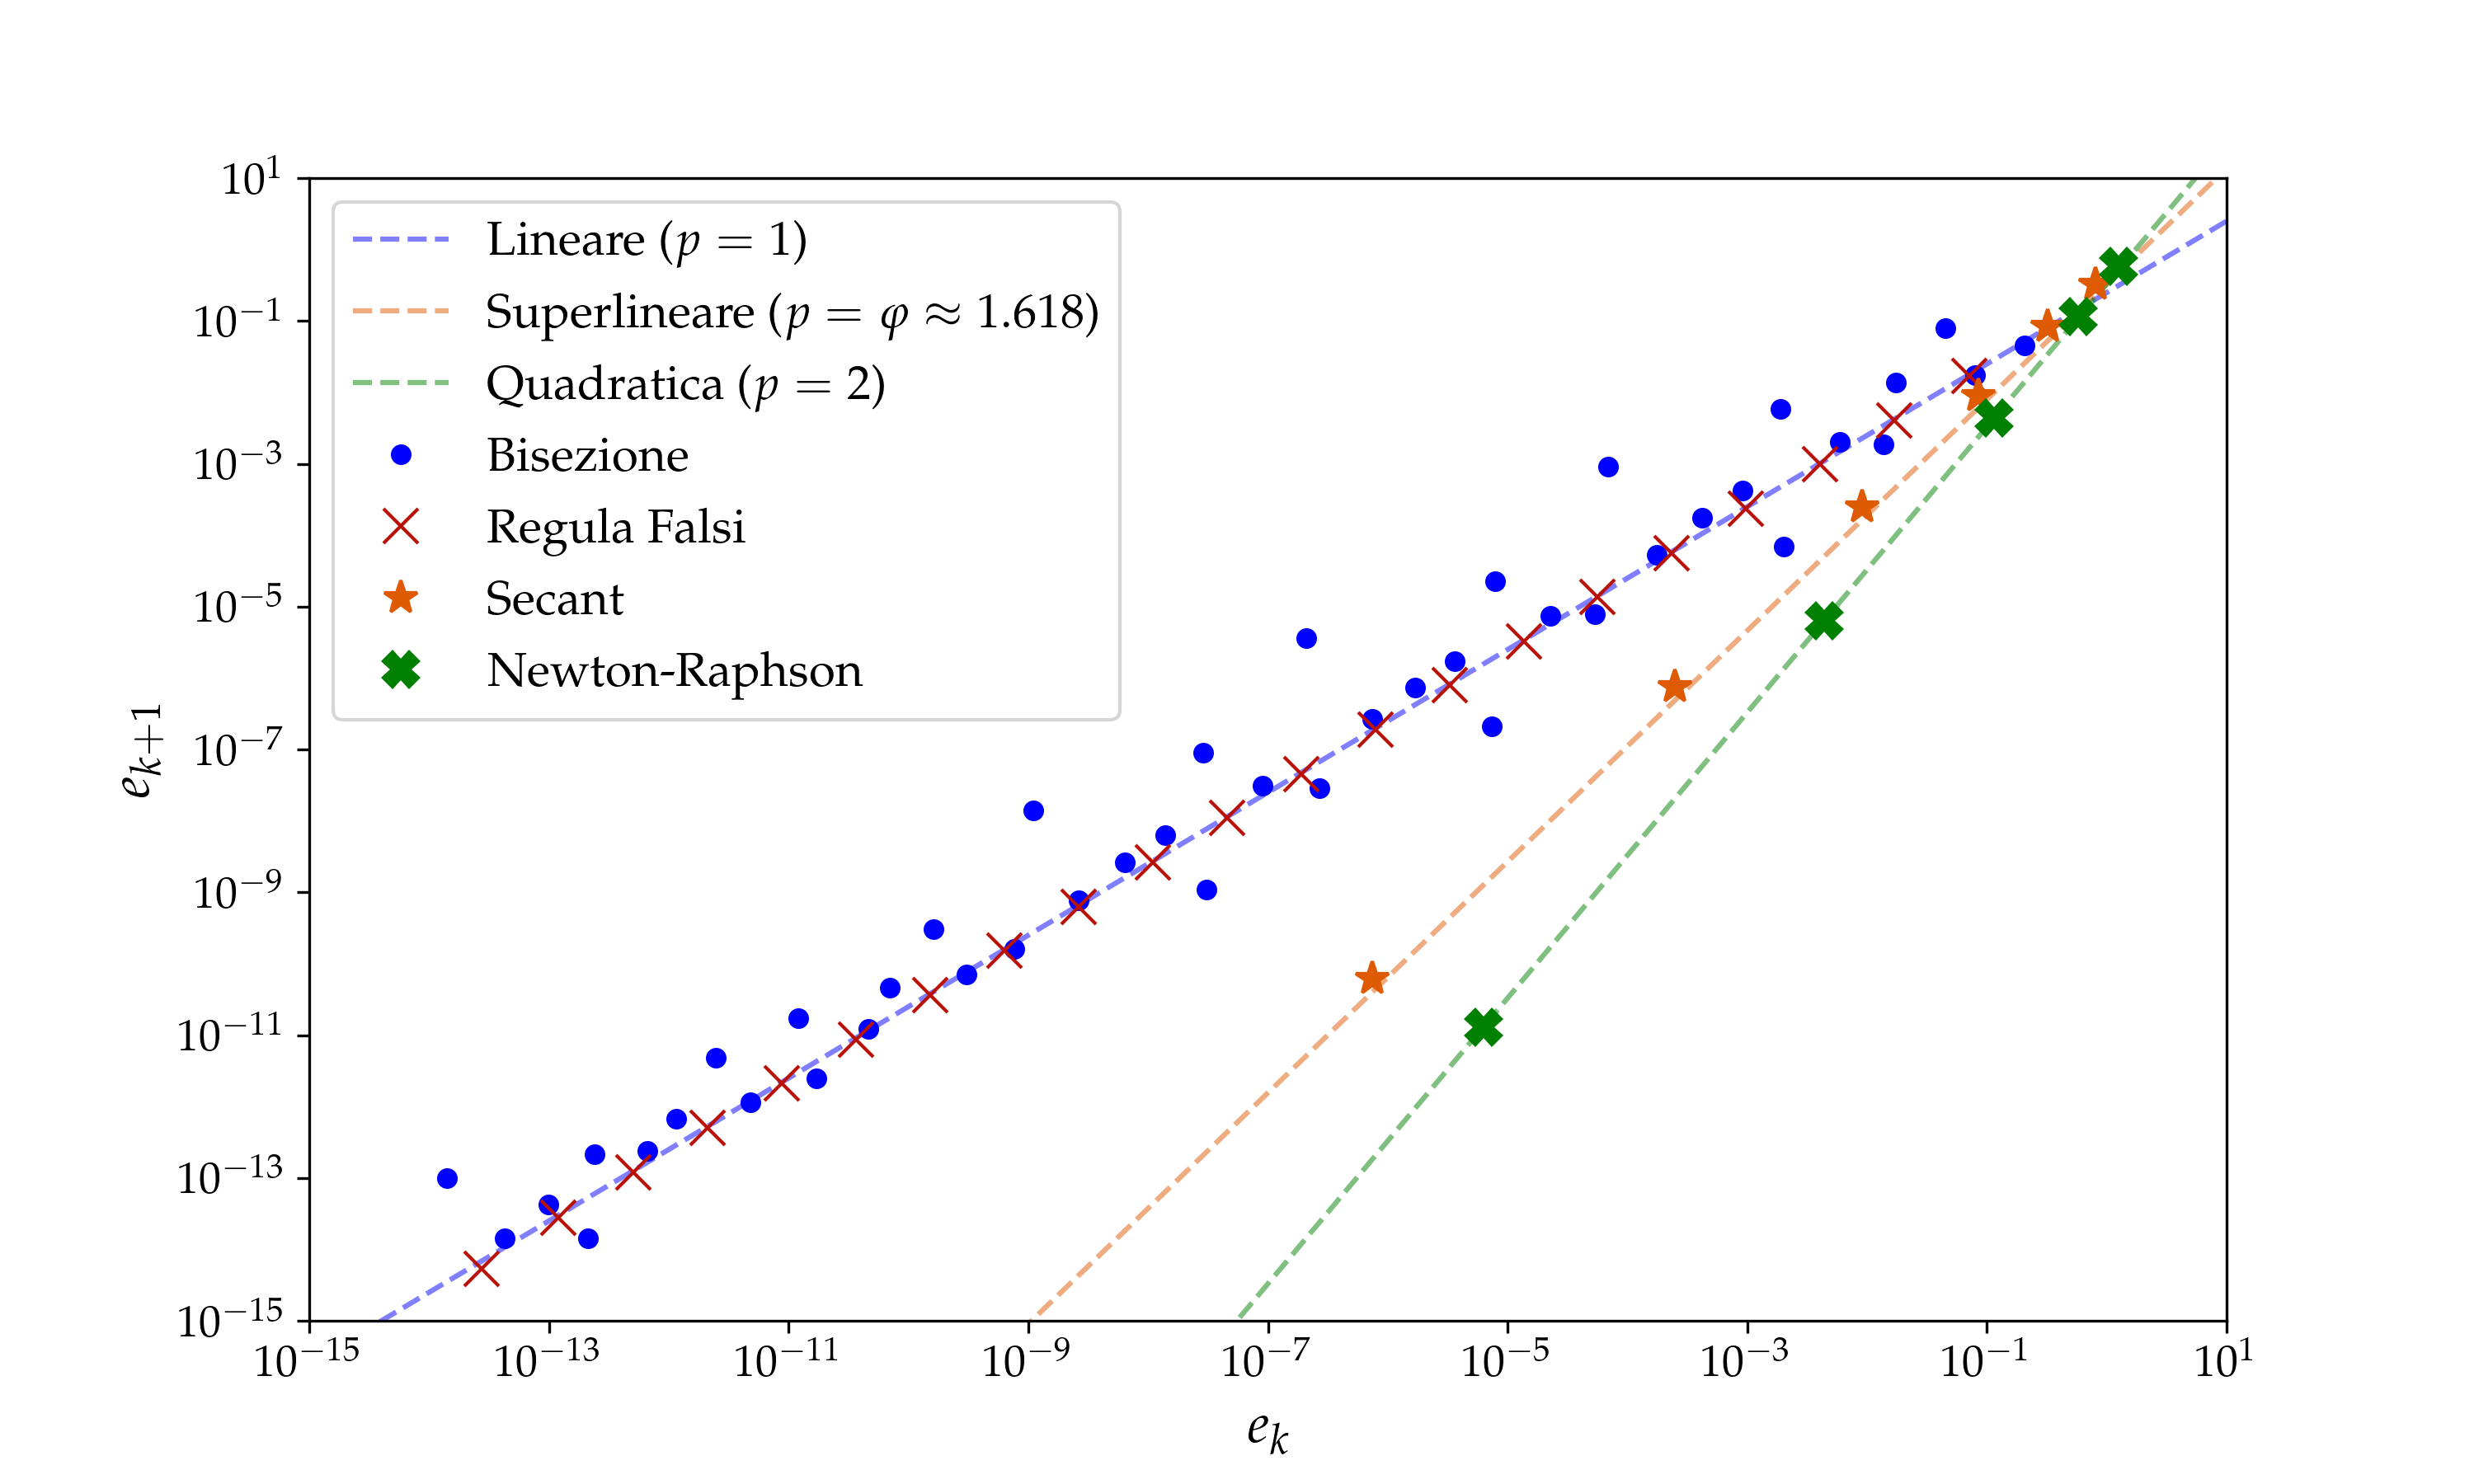
\includegraphics[width=0.95\linewidth]{images/14/scat_lines_even.png}
    \caption{l'andamento della convergenza unificato in un unico plot per tutti gli algoritmi. Tratteggiate le rette che segnano gli andamenti asintotici previsti e su cui, rispettivamente, si appoggiano i metodi. Per l'intestazione degli assi vale la stessa approssimazione di Fig.\ref{fig: fit Bis}.}
    \label{fig: confr even}
\end{figure}

\begin{figure}[H]
    \centering
    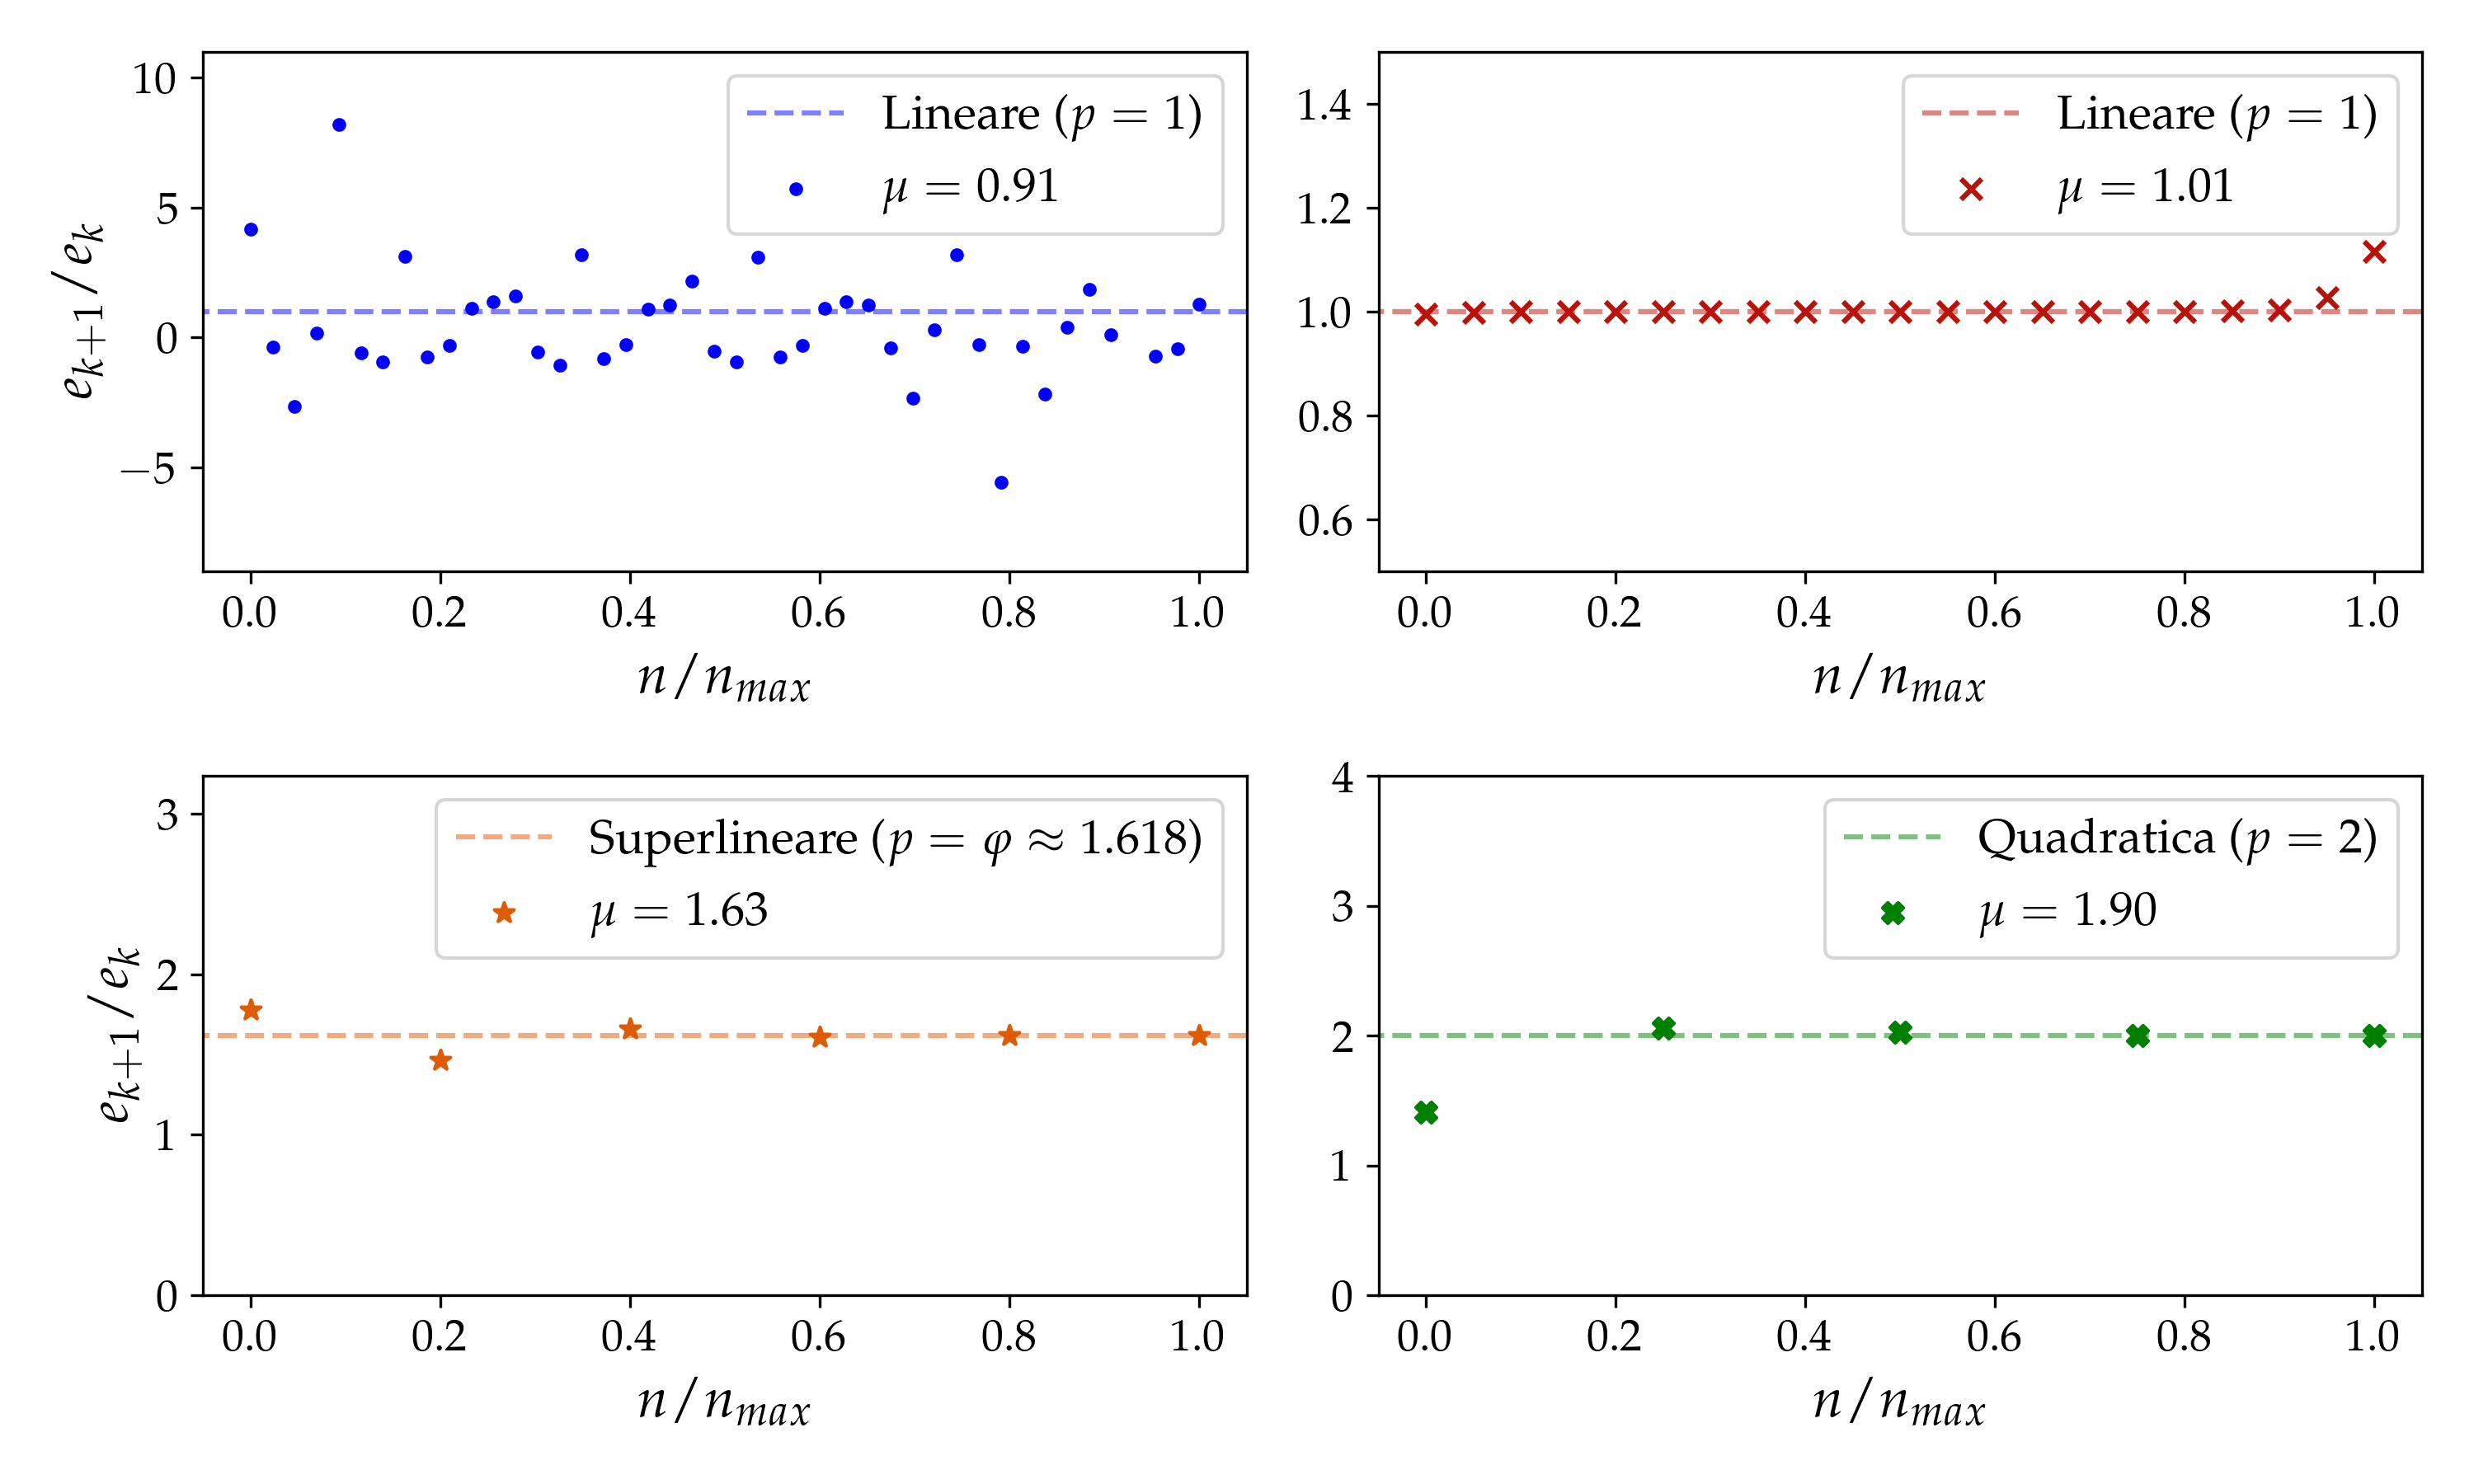
\includegraphics[width=0.9\linewidth]{images/14/single_scat_even.png}
    \caption{Nell'immagine sono separati i diversi andamenti dei punti organizzati nei plot in maniera da evidenziare l'aderenza proprio al $p$, fattore di scaling, aspettato. Sull'asse delle ascisse si leggono le iterazioni, normalizzate in maniera che sia uniforme la visualizzazione a prescindere della velocità di convergenza del singolo metodo. Sulle ordinate il rapporto $e_{n+1}/e_n$, che corrisponde al coefficiente angolare della retta nella Fig. \ref{fig: confr even} e che vediamo globalmente aderente al valore atteso. Viene indicato con $\mu$ il valore medio delle ordinate.}
    \label{fig: even mean}
\end{figure}


\begin{multicols}{2}
\begin{figure}[H]
    \centering
    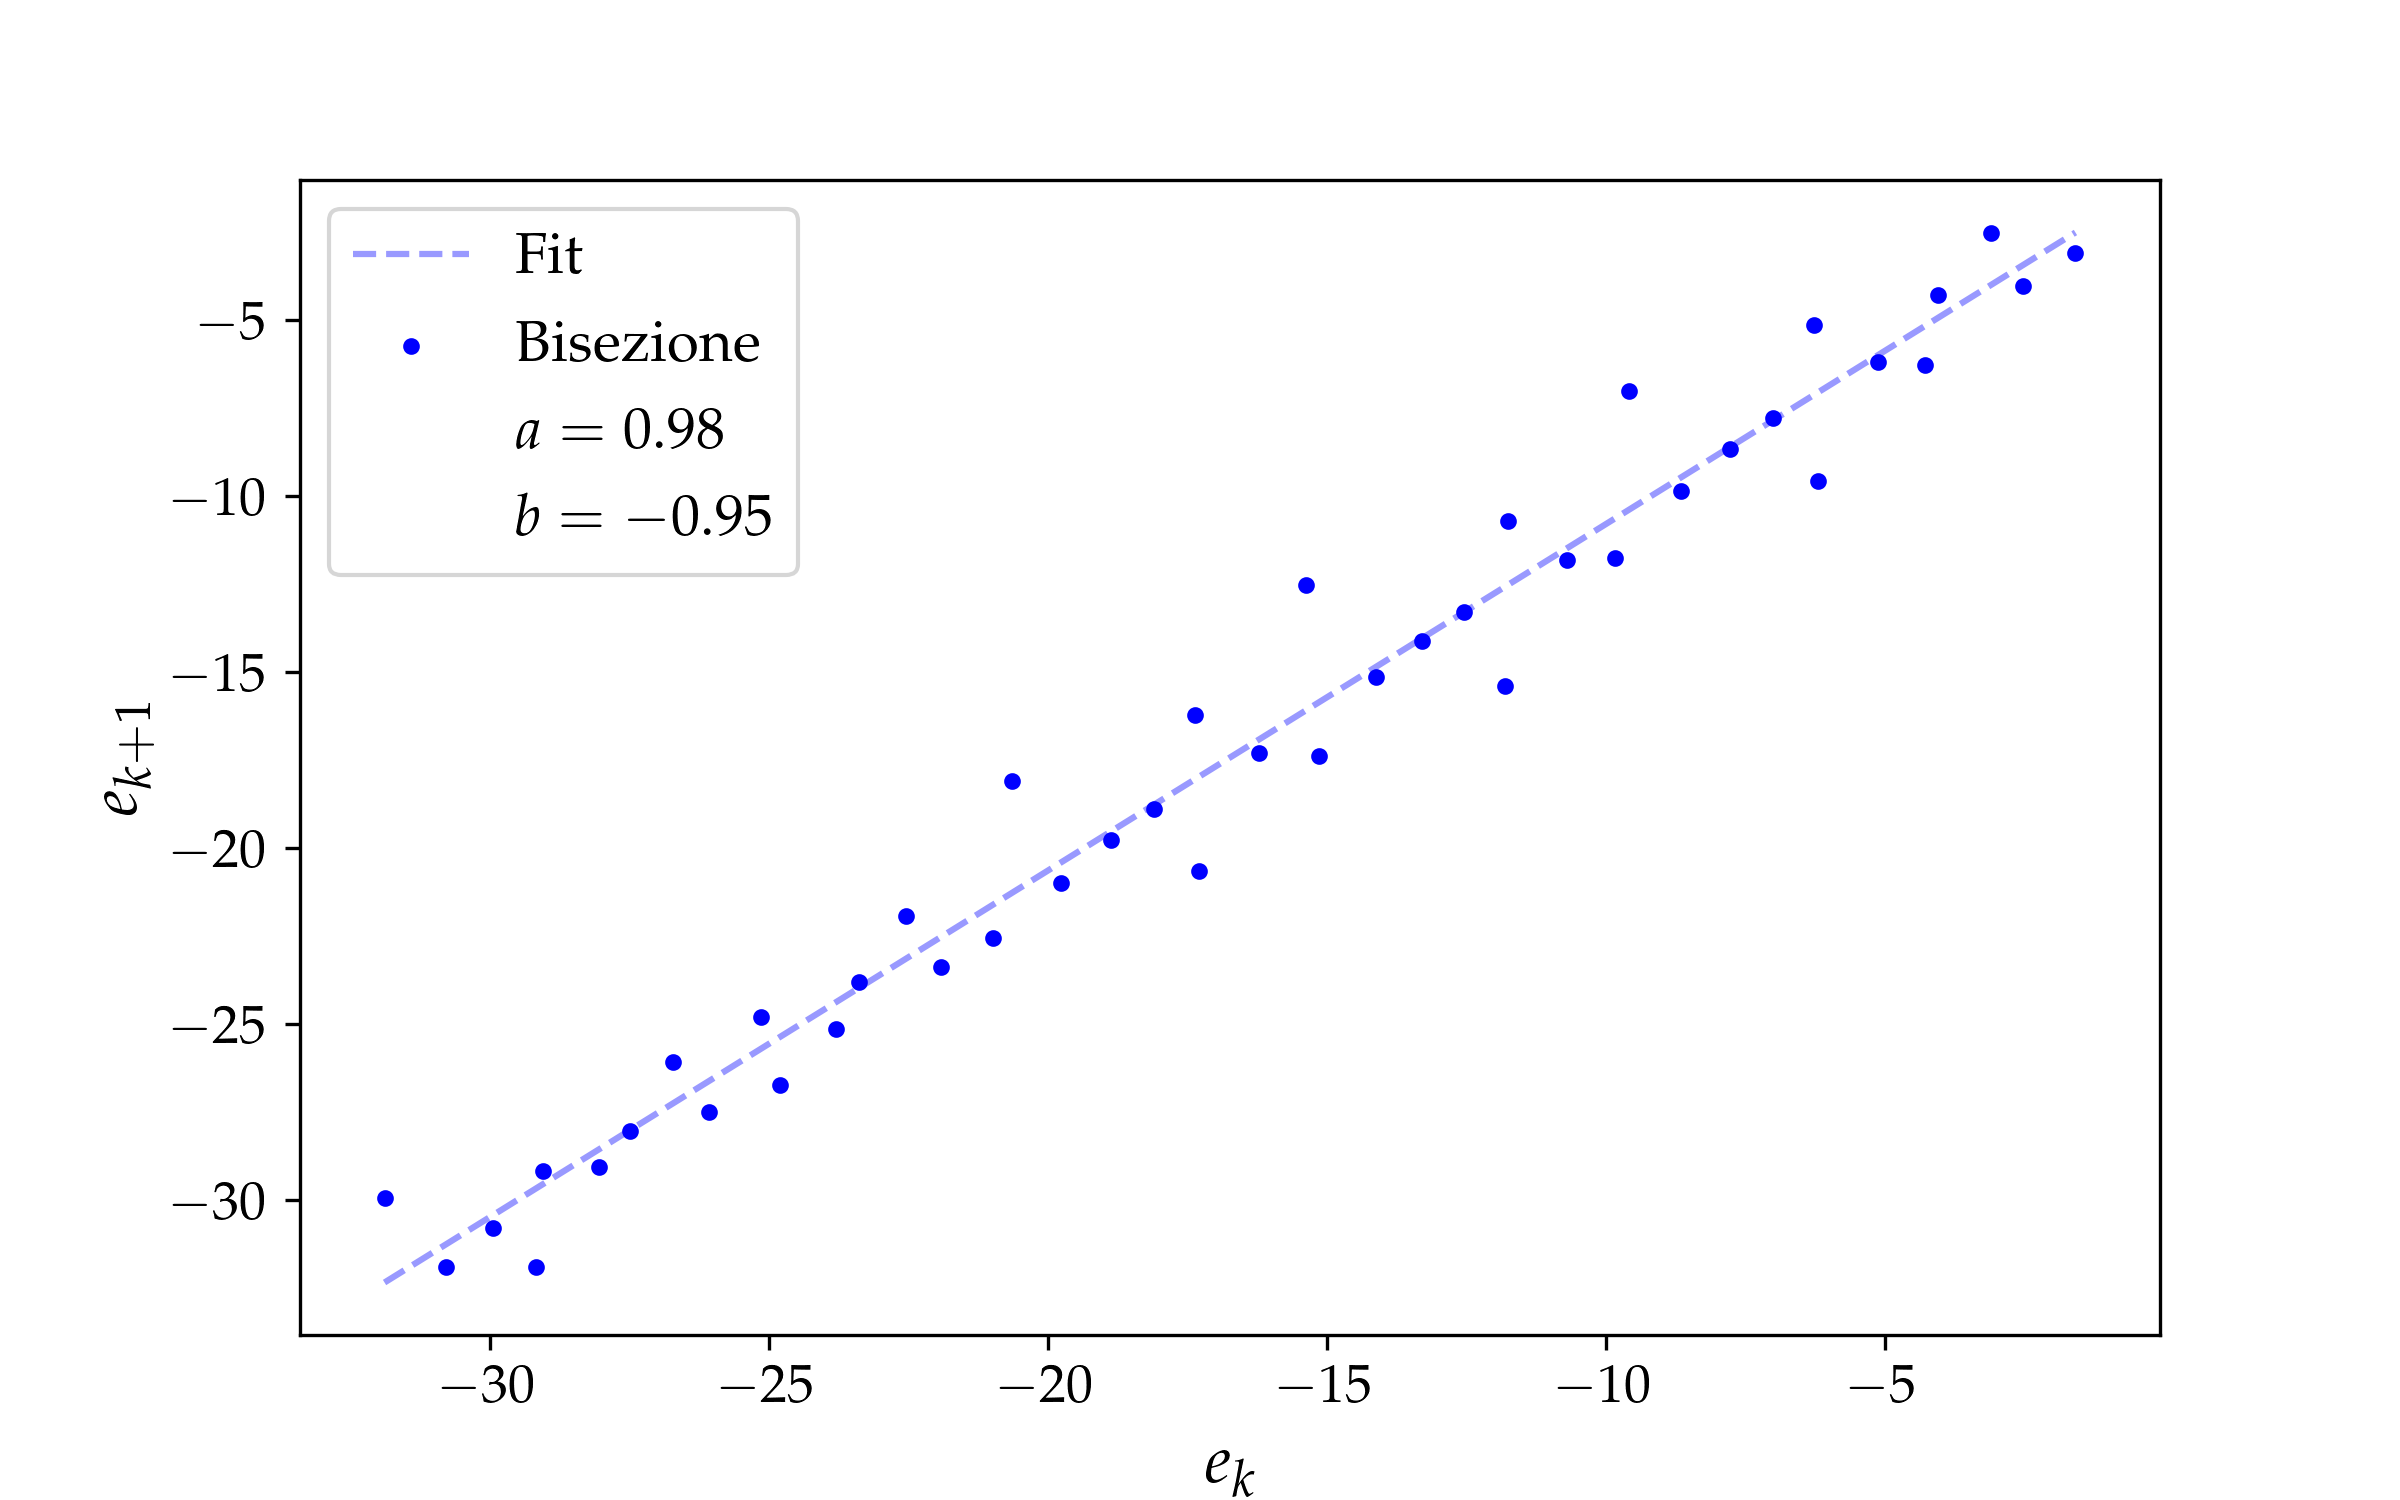
\includegraphics[width=\linewidth]{images/14/fit_Bisezione.png}
    \caption{Fit delle iterazioni di Bisezione per stima del parametro di scaling.}
    \label{fig: bisezione_fit}
\end{figure}

\begin{figure}[H]
    \centering
    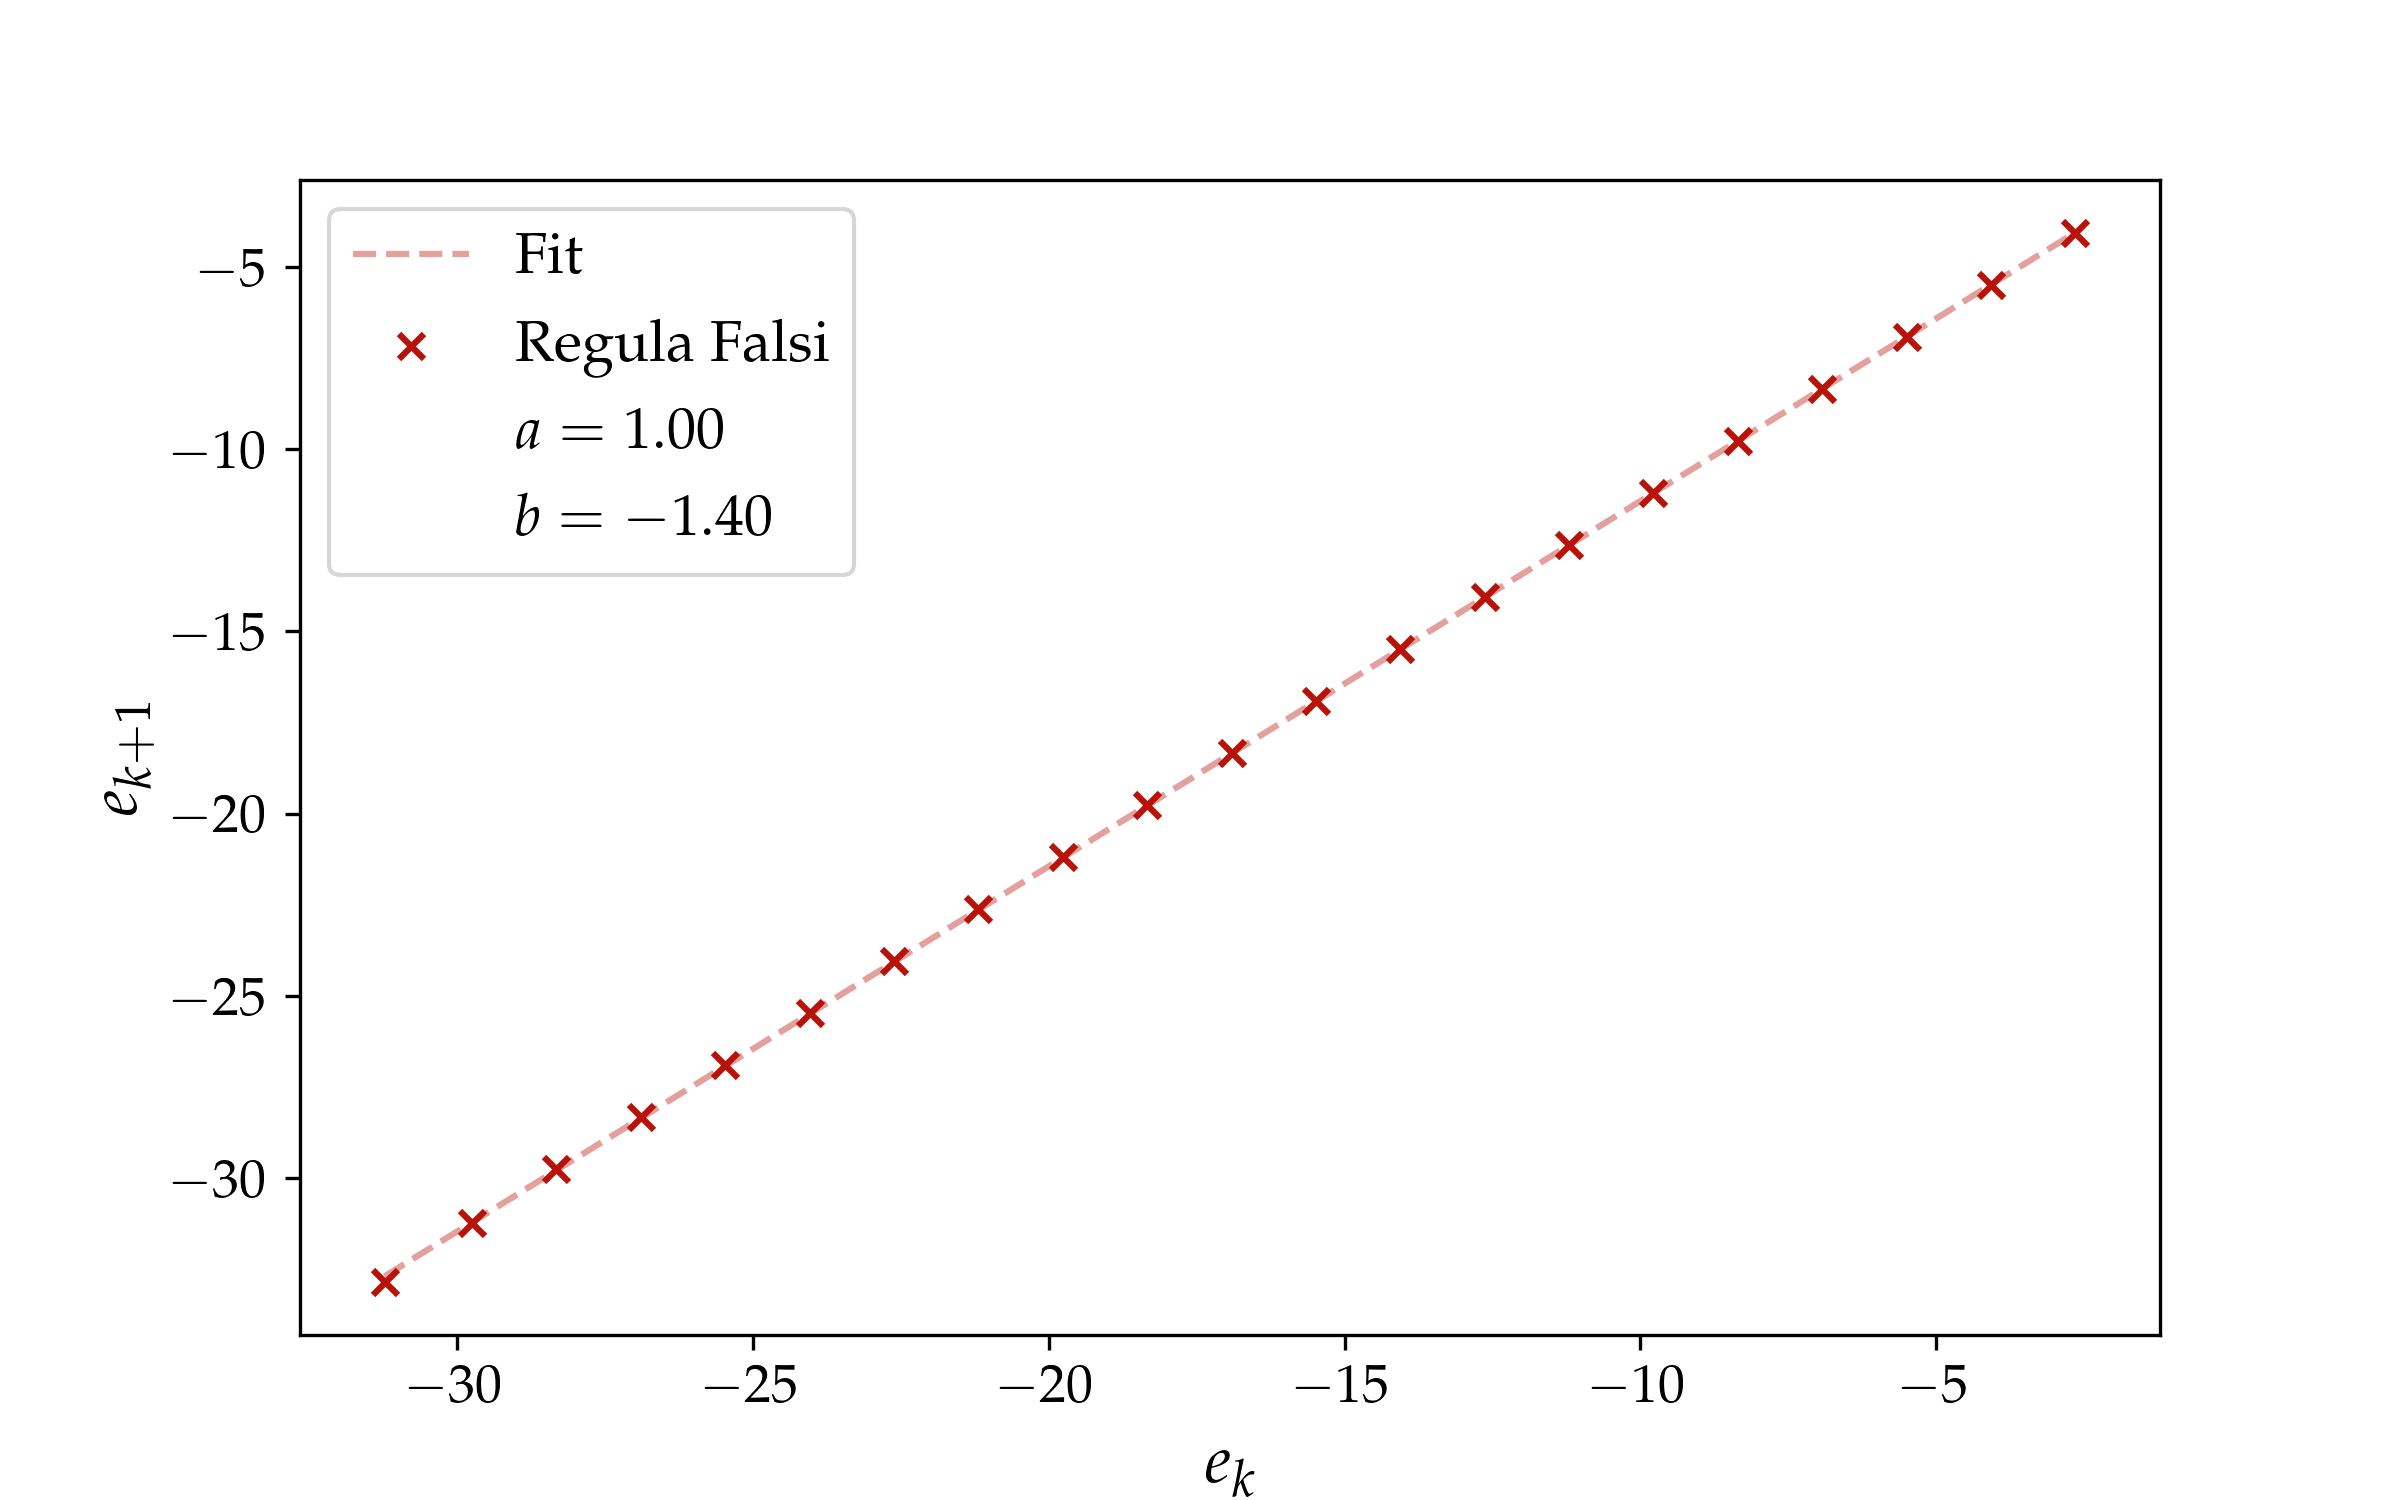
\includegraphics[width=\linewidth]{images/14/fit_Regula Falsi.png}
    \caption{Fit delle iterazioni di Regula Falsi per stima del parametro di scaling.}
    \label{fig: reg_fit}
\end{figure}
\end{multicols}

\begin{multicols}{2}
\begin{figure}[H]
    \centering
    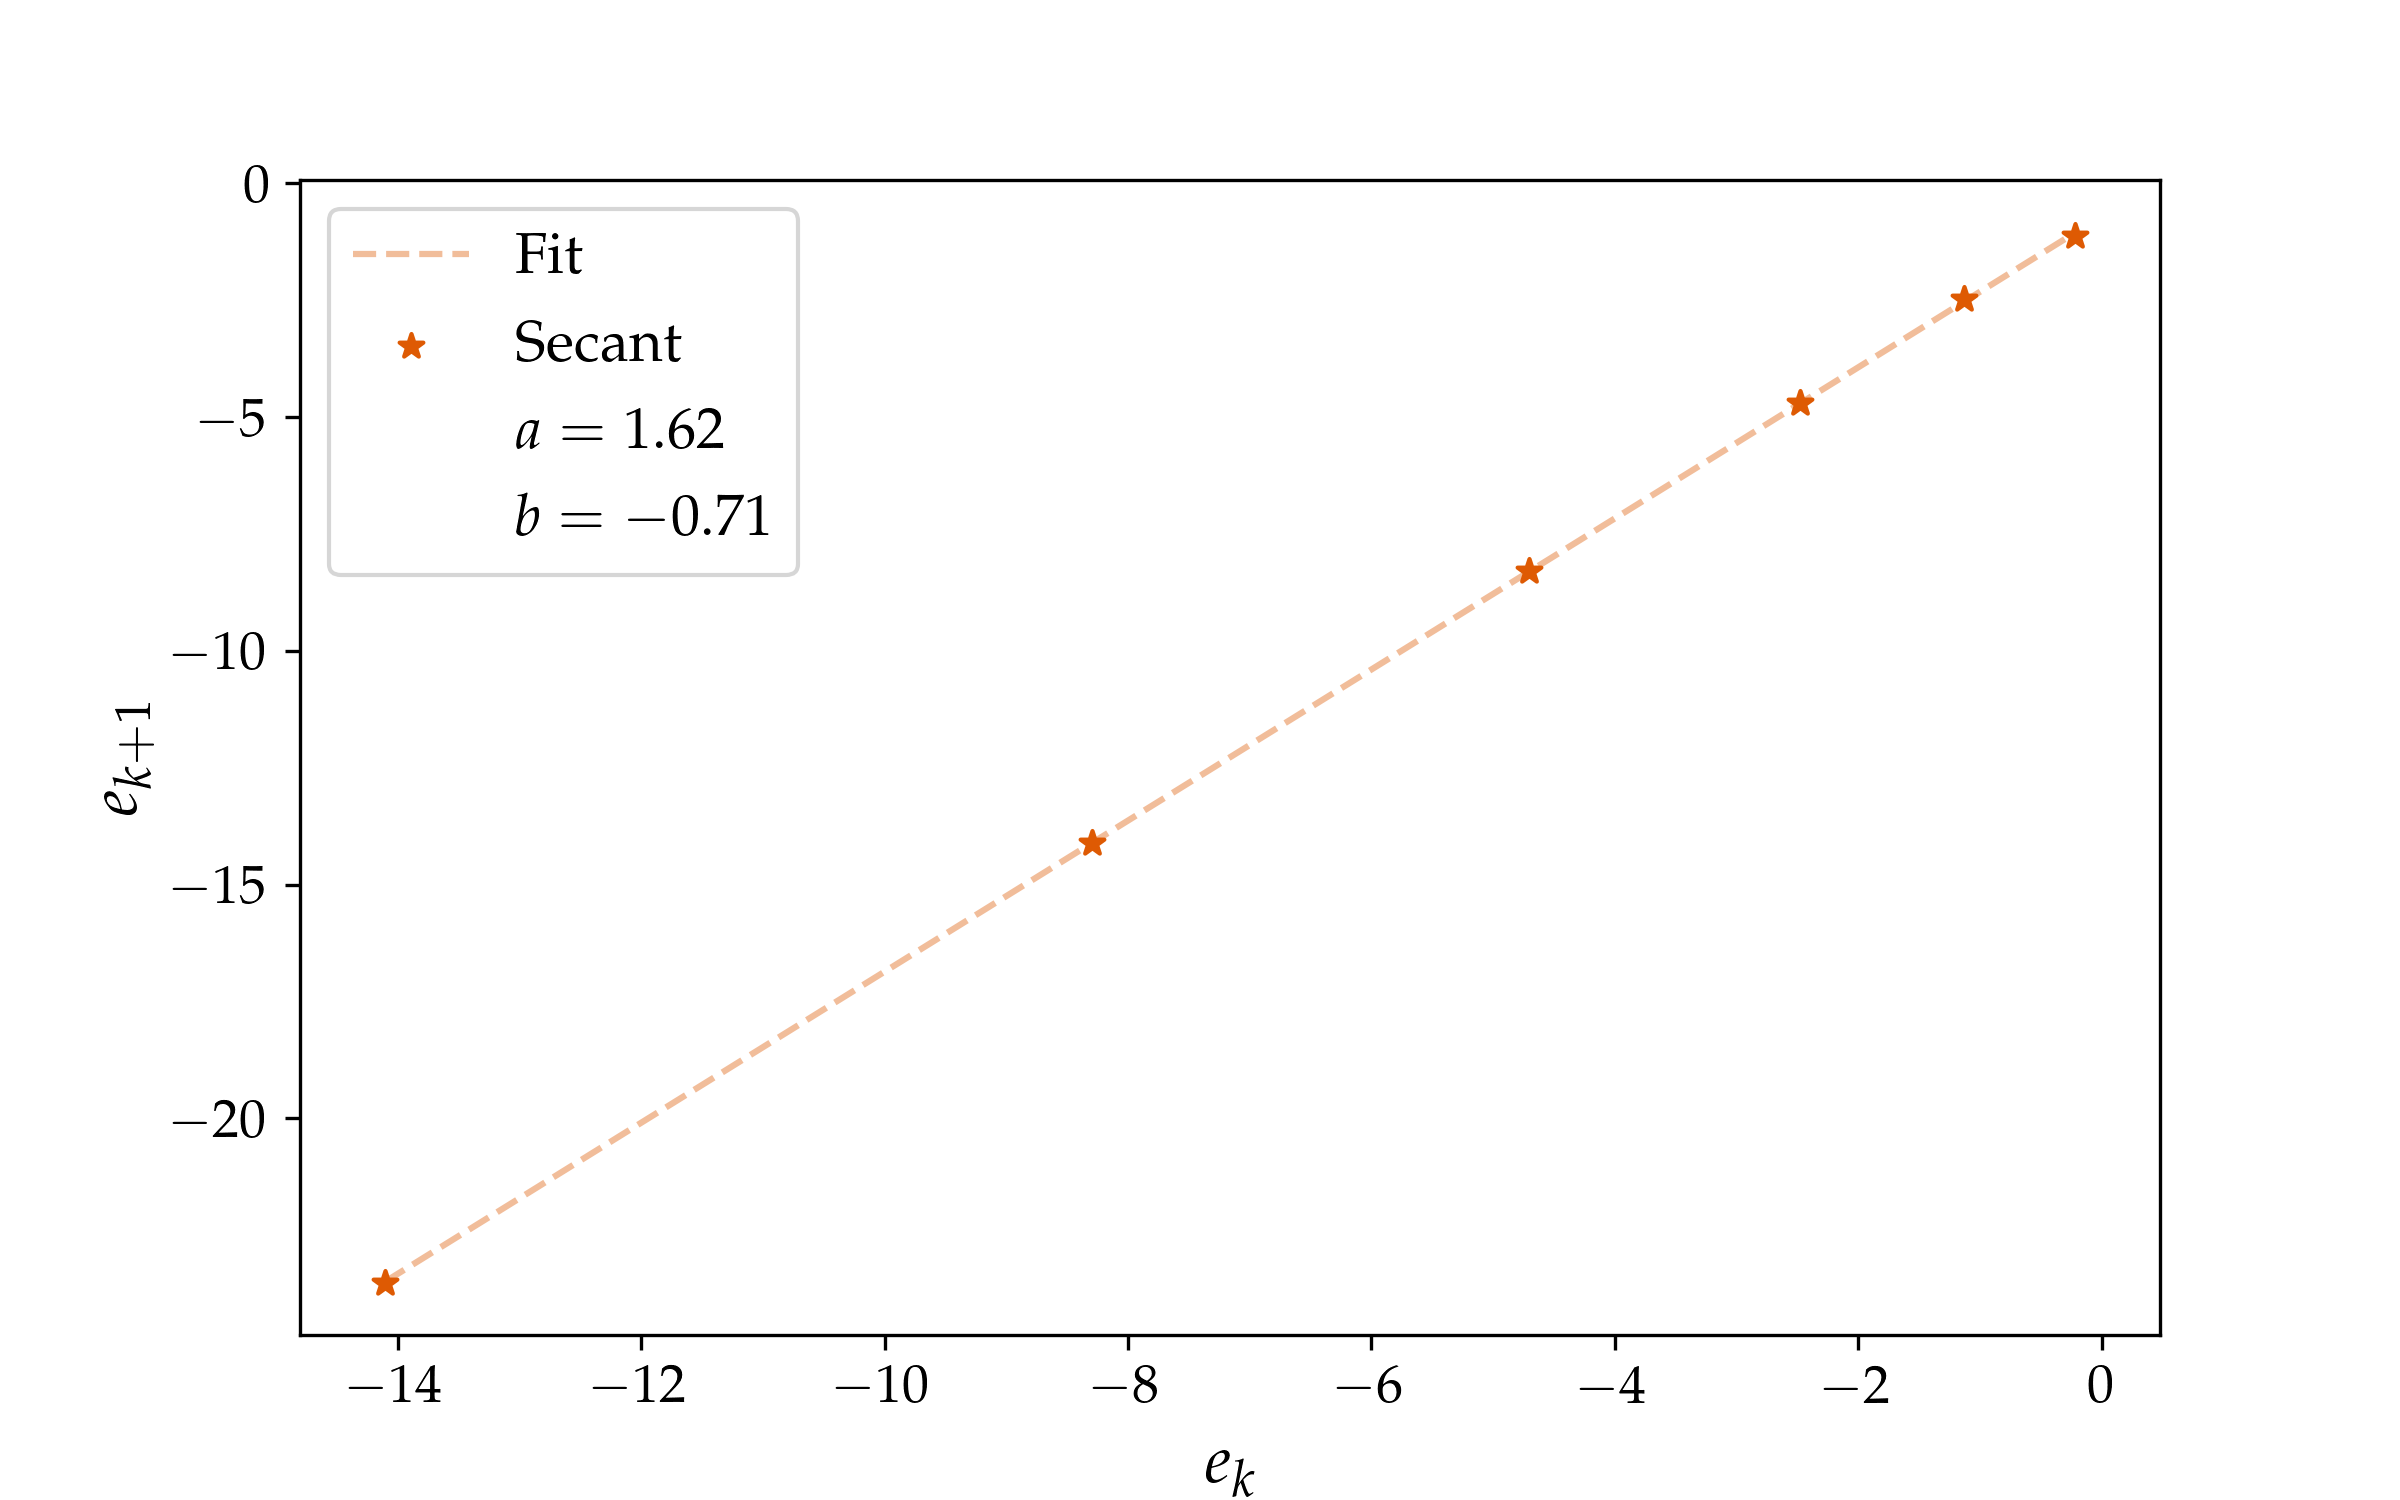
\includegraphics[width=\linewidth]{images/14/fit_Secant.png}
    \caption{Fit delle iterazioni di Secanti per stima del parametro di scaling.}
    \label{fig: sec_fit}
\end{figure}

\begin{figure}[H]
    \centering
    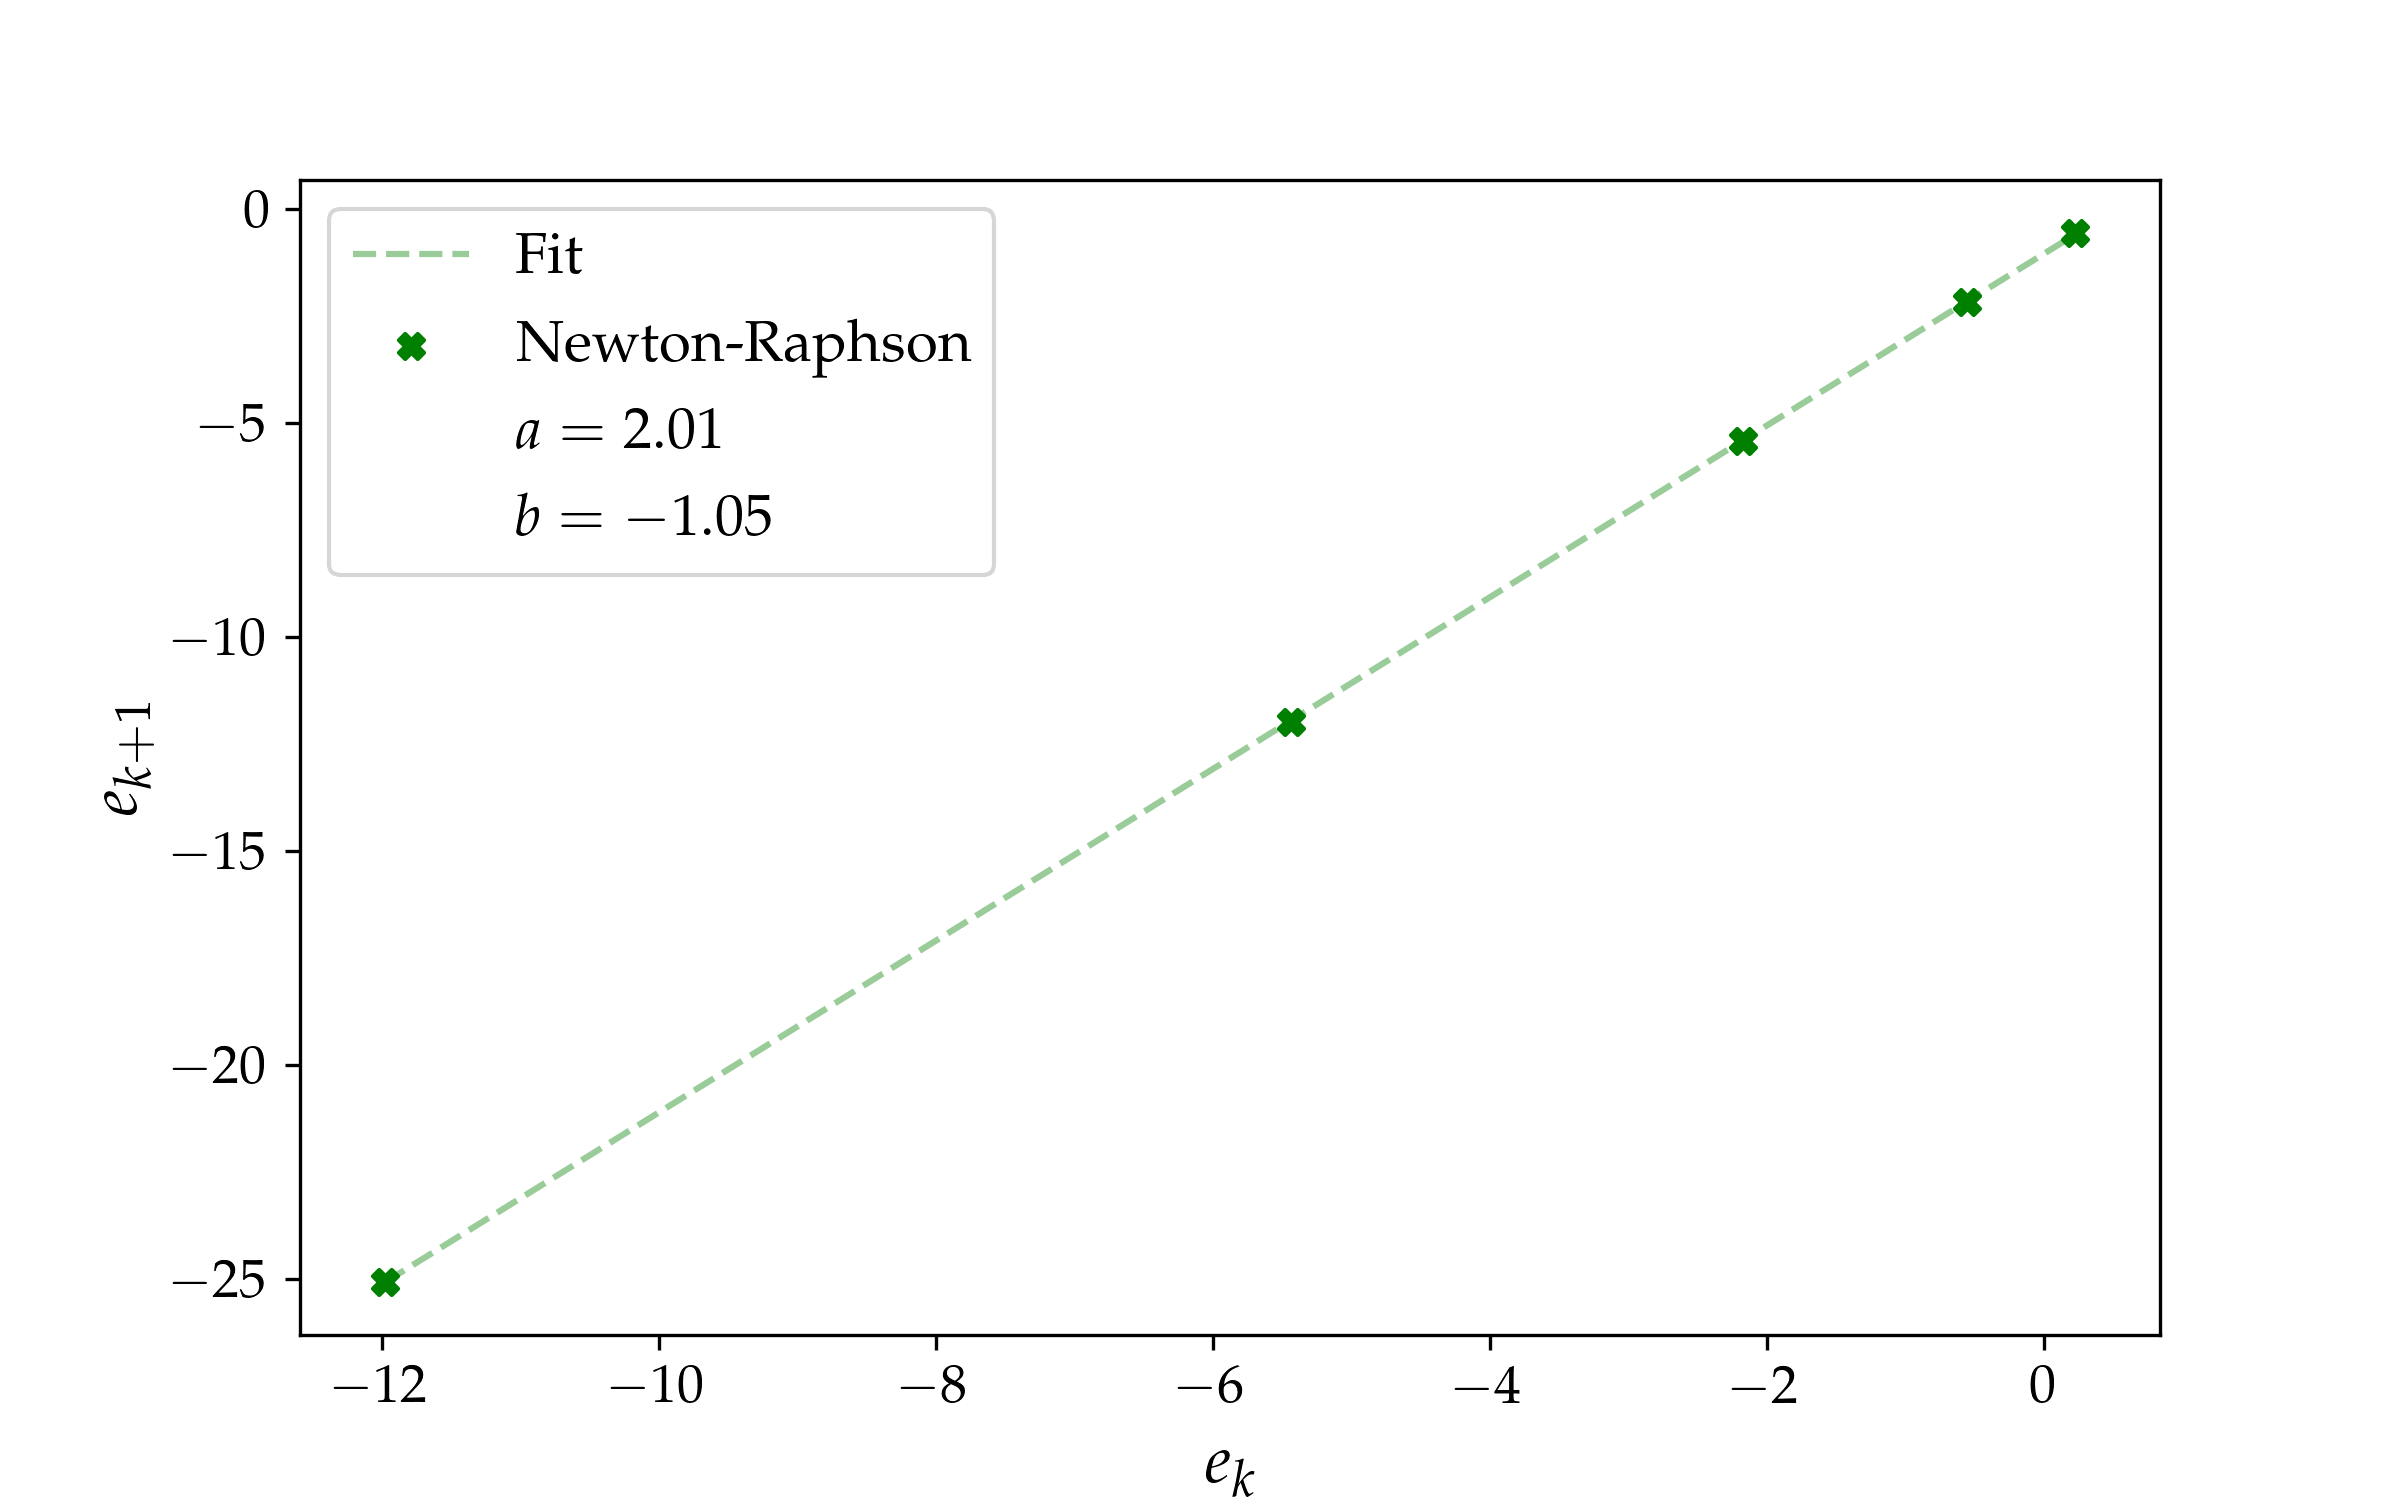
\includegraphics[width=\linewidth]{images/14/fit_Newton-Raphson.png}
    \caption{Fit delle iterazioni di Newton-Raphson per stima del parametro di scaling.}
    \label{fig: NR_fit}
\end{figure}

\end{multicols}

Le previsioni teoriche sui differenti rate di convergenza vengono quindi confermate dai fit.

\bigskip\noindent
Un ultima indagine è quella che si propone nel contesto della convergenza di N-R: si studia la storia dell'algoritmo in funzione dello \textit{starting point} $x_0 \in [-5.2,-5.0]$, campionando quattro punti in questo intervallo.\\
In Fig. \ref{fig: cn_fail} vediamo come la radice converga al valore approssimativo di $c_{true}\approx - 7.71$, tranne per il caso di $x_0=-5.0$: in questo caso l'algoritmo passa all'essere divergente, aumentando l'errore ad ogni step. 

\begin{elegantcode}
f(-5.07) = 13432.21
df(-5.07) = 9148811.79

f(-5.00) = -308.91
df(-5.00) = 4644.23
\end{elegantcode}

\noindent Il confronto con la Fig. \ref{fig: f even} chiarisce che sul lato sinistro della singolarità, che si trova molto vicina al punto $x=-5$ , la funzione è positiva per $x > 7.71$, mentre ha cambiato segno per $x=-5$, indicazione che ci siamo spostati sul lato destro del punto di discontinuità, ma con stesso segno della derivata. L'utilizzo della retta tangente per trovare la radice ci porterà solamente ad allontanarci ancora di più dalla radice vera, portando inevitabilmente alla divergenza del metodo così impostato.\\
In Fig. \ref{fig: errn_fail} un secondo plot che evidenzia invece l'errore relativo alla radice n-esima, confrontando la \textit{guess} con la migliore stima, che viene fatta trovando lo zero con N-R e $x_0=-7.0$.



\begin{figure}[H]
    \centering
    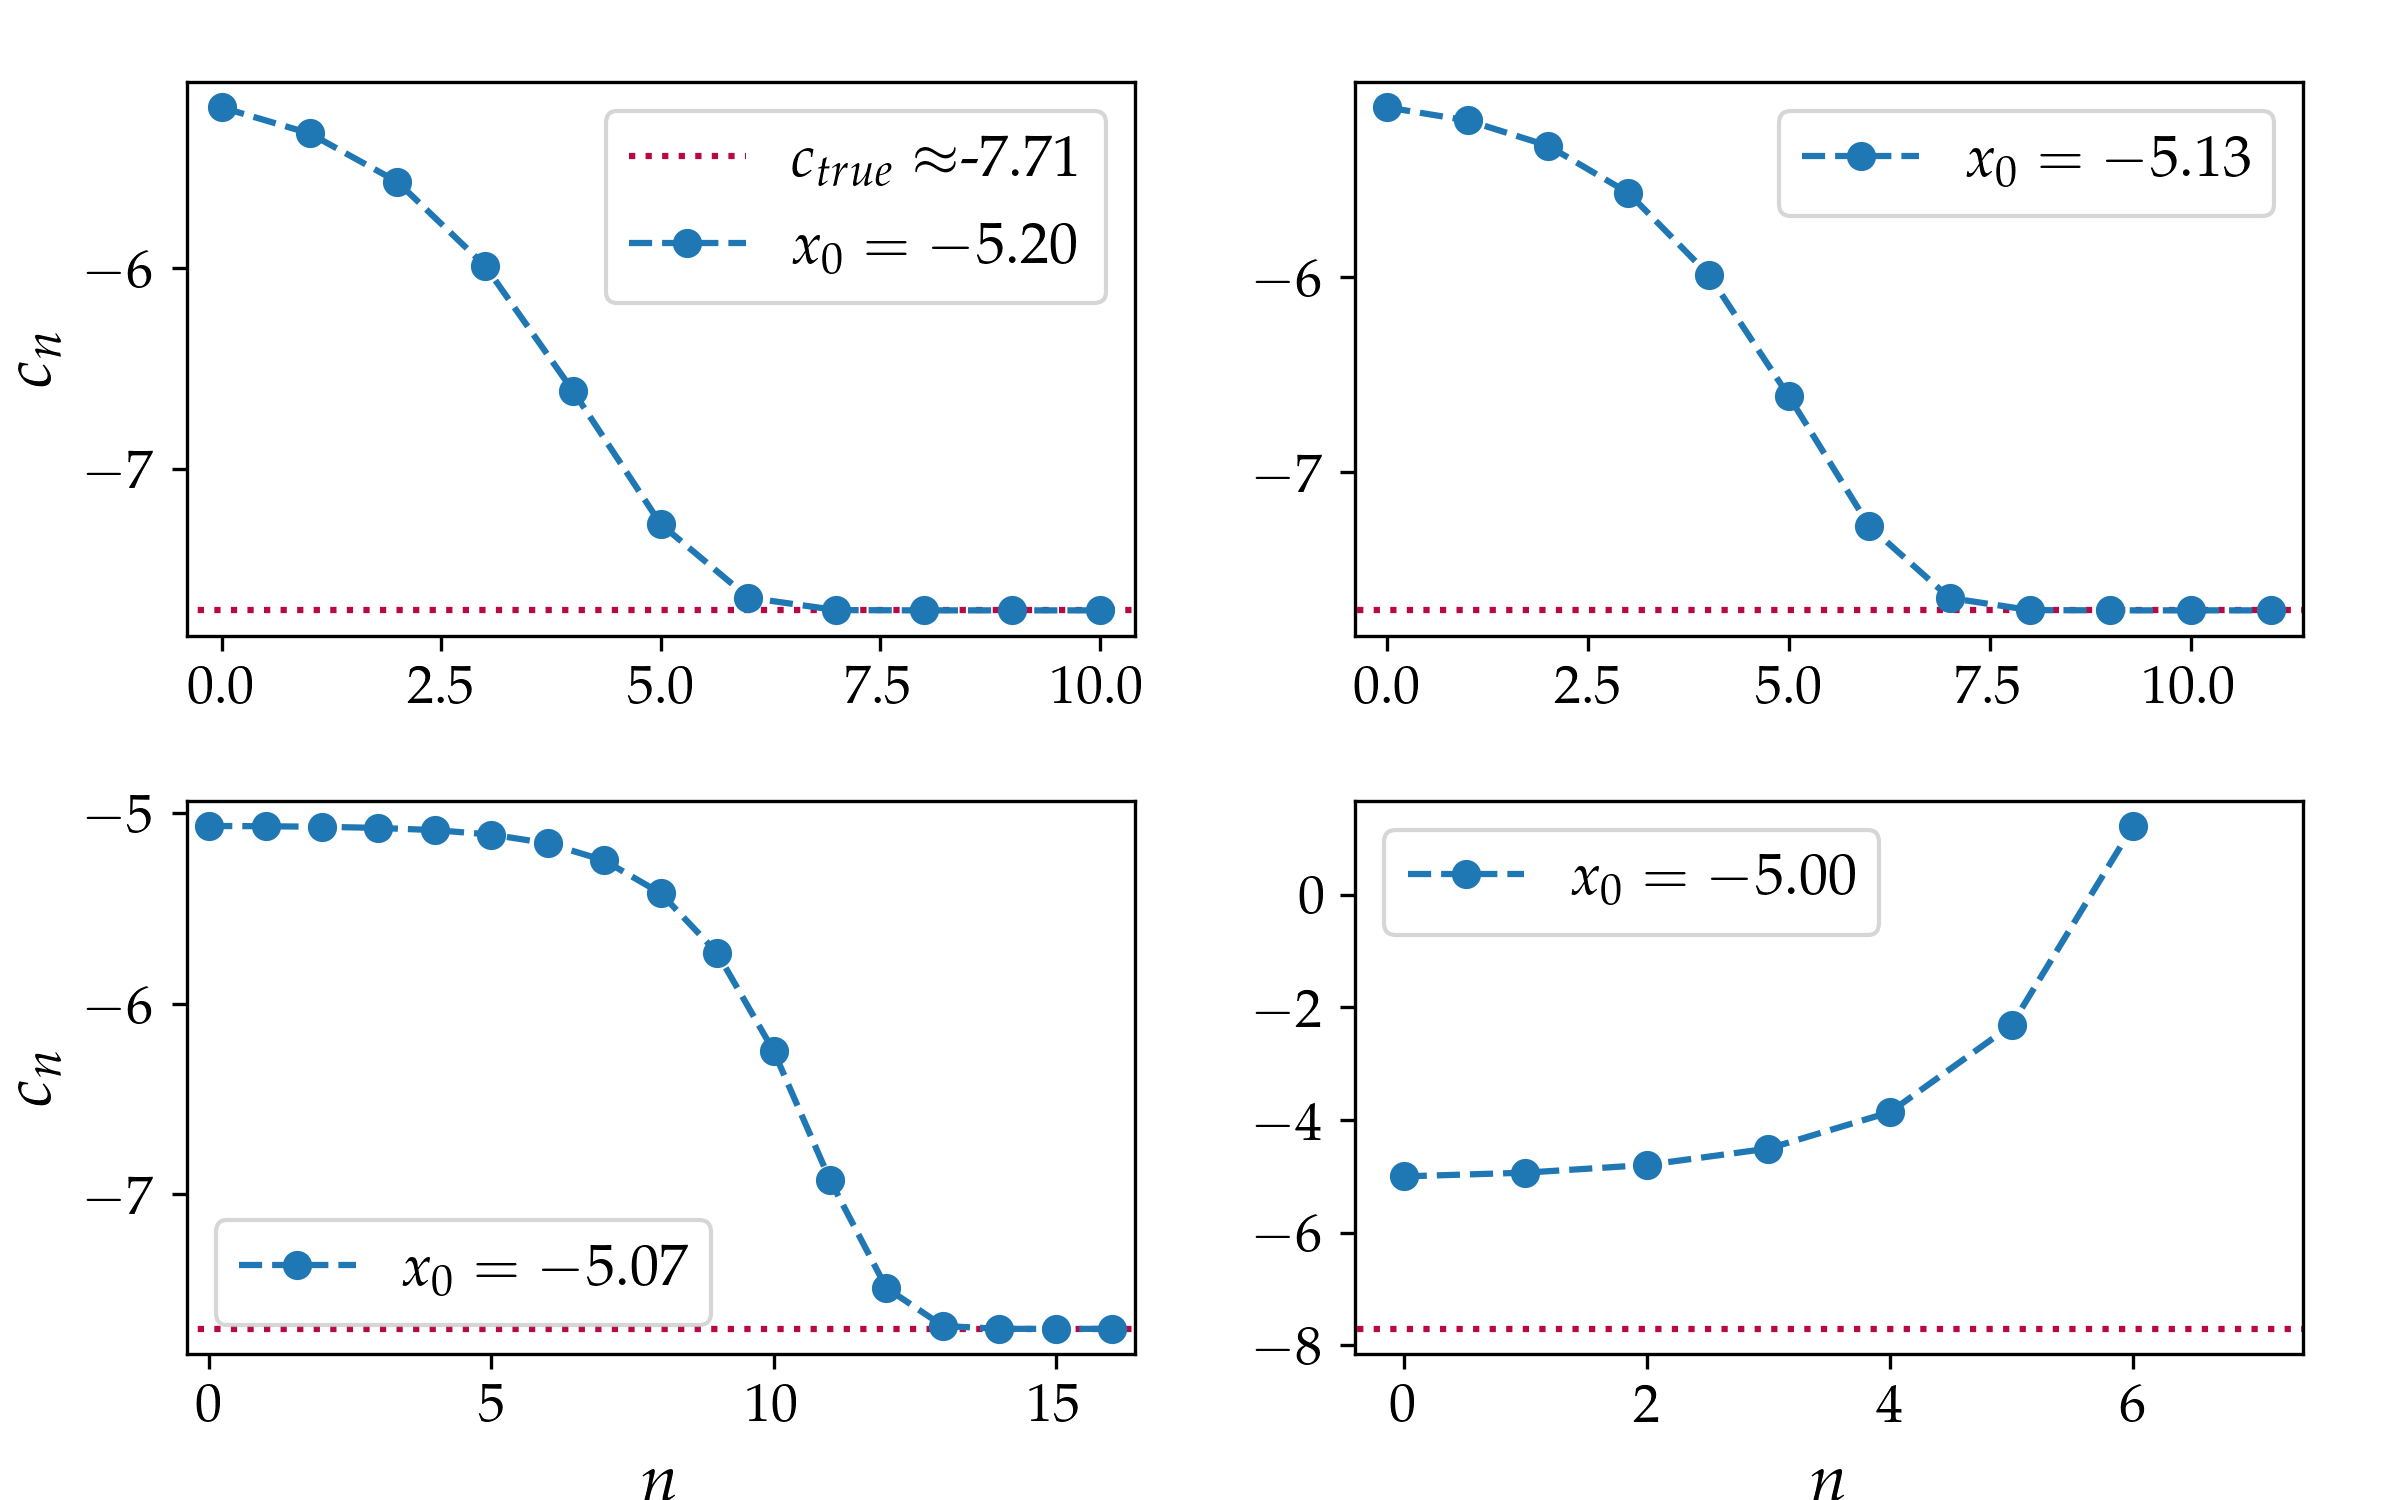
\includegraphics[width=0.8\linewidth]{images/14/cn_fail.png}
    \caption{La storia della radice n-esima di N-R al variare dello \textit{starting point} $x_0$.}
    \label{fig: cn_fail}
\end{figure}
\begin{figure}[H]
    \centering
    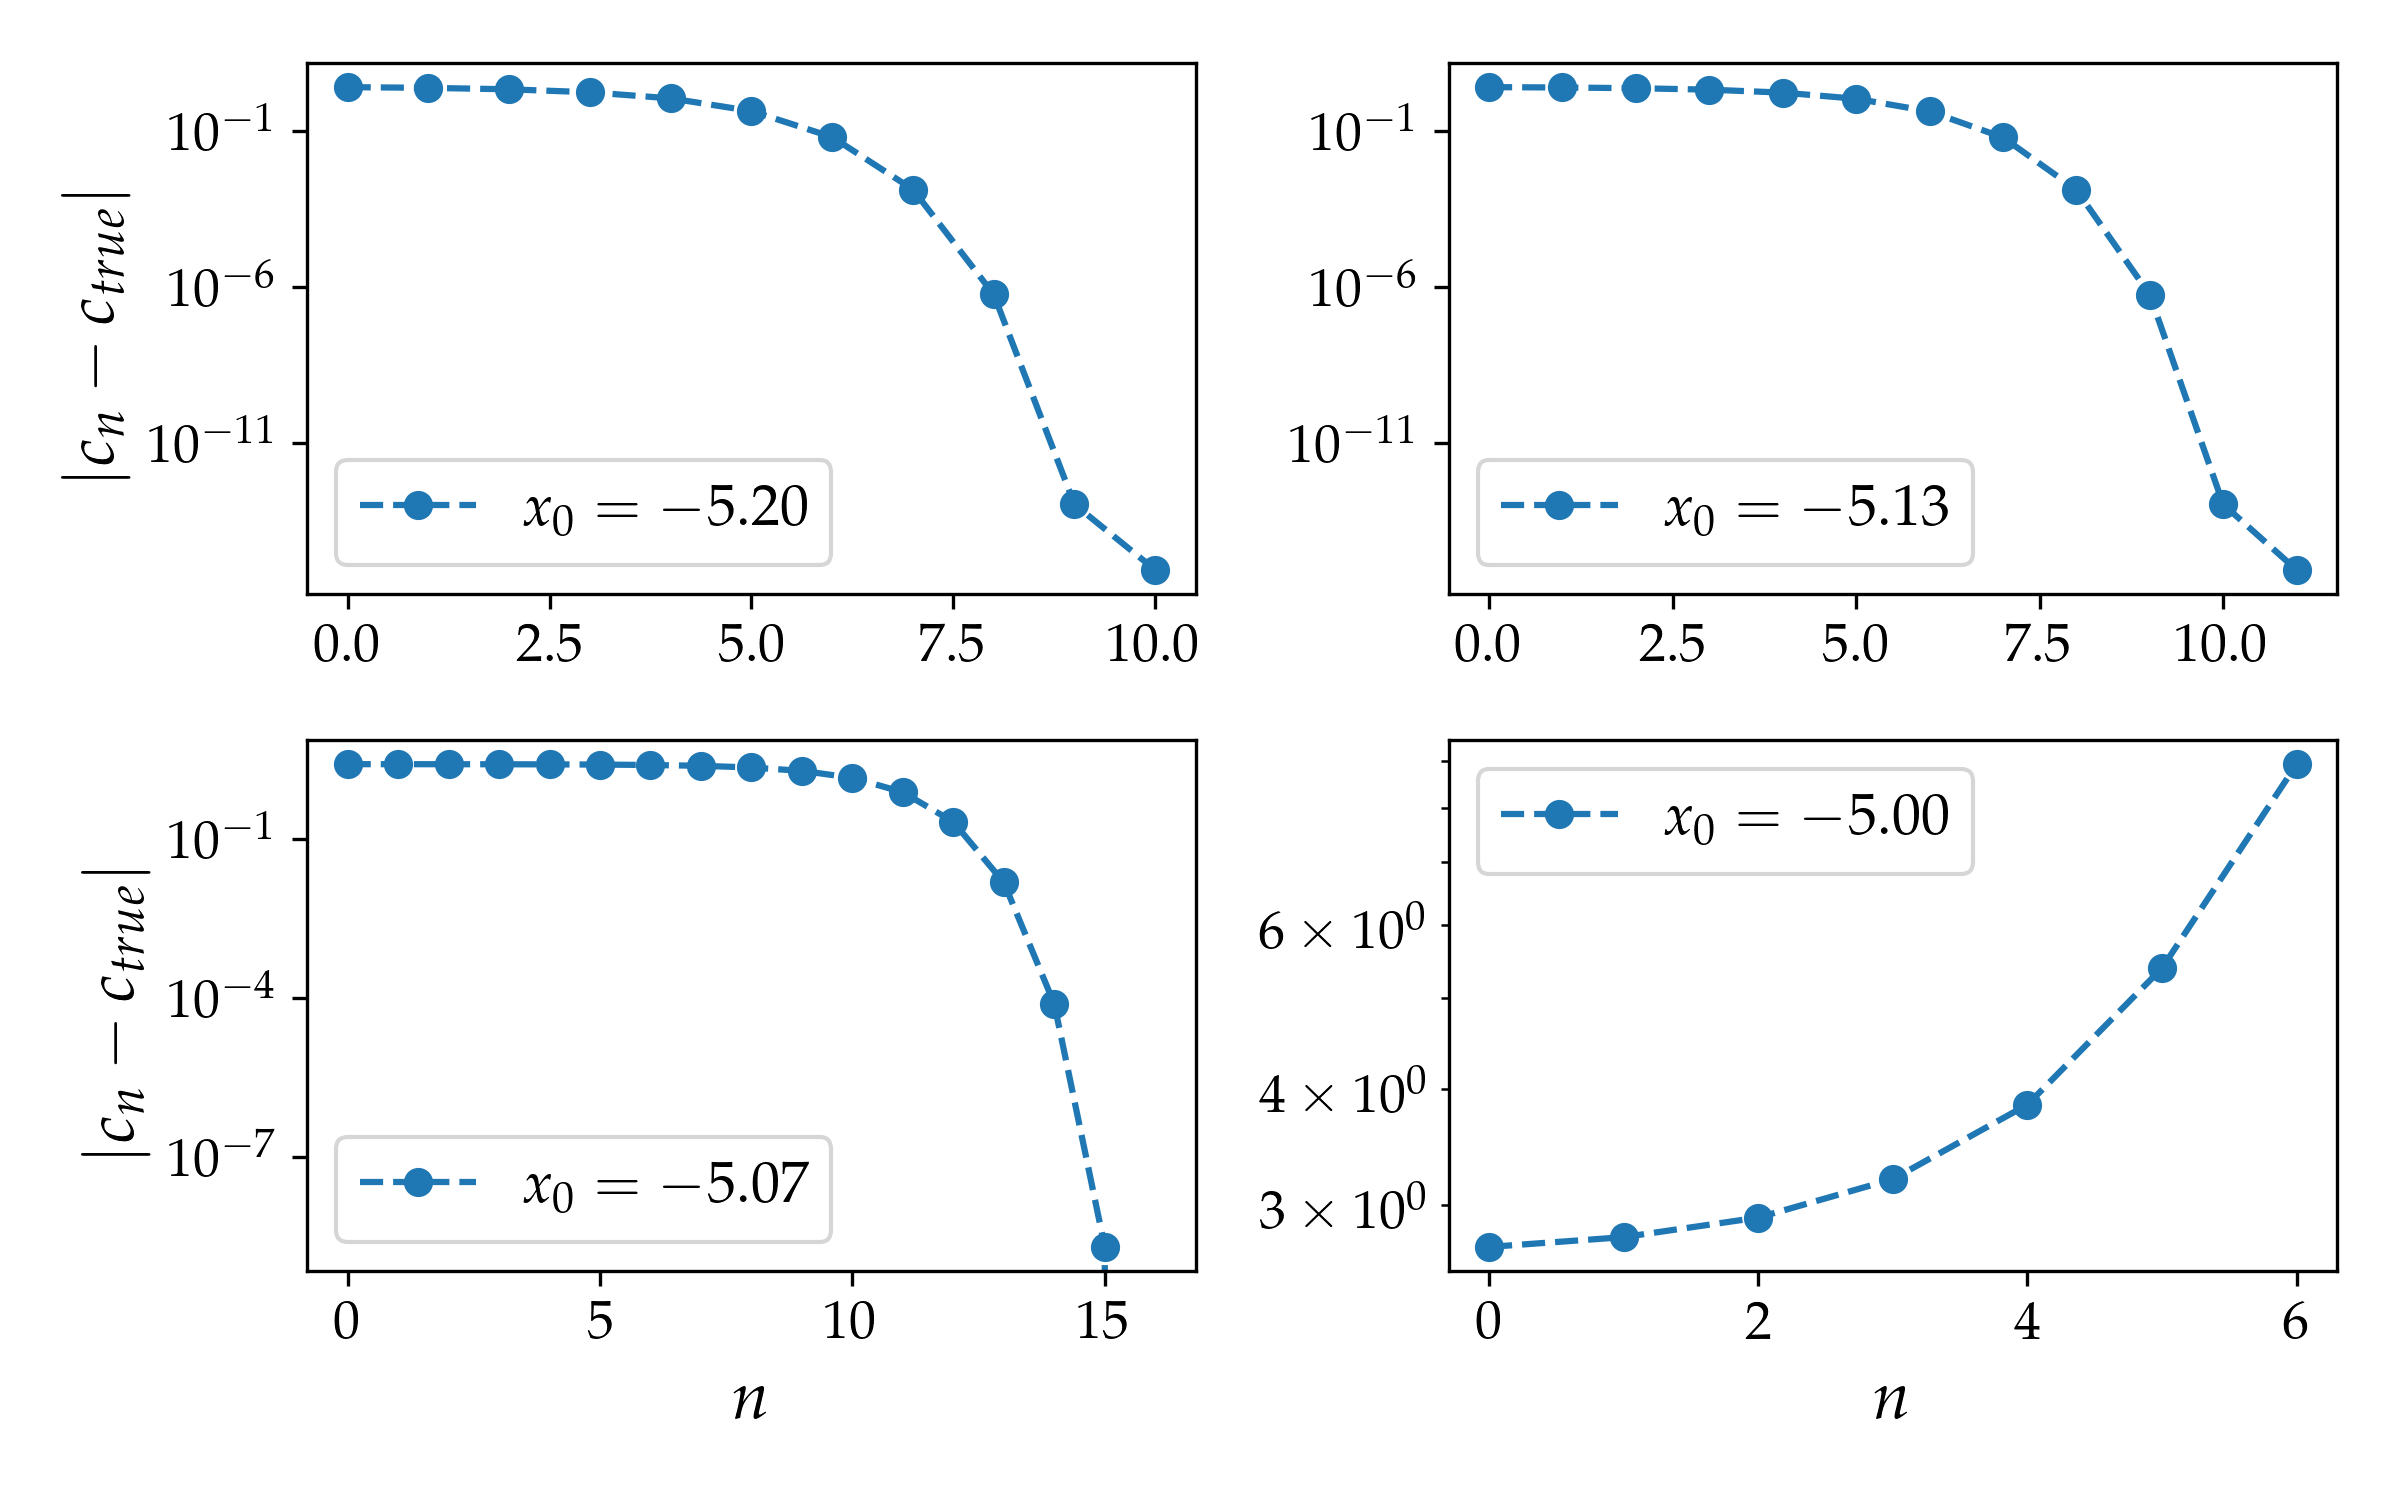
\includegraphics[width=0.8\linewidth]{images/14/errn_fail.png}
    \caption{La storia dell'errore sulla radice n-esima di N-R al variare dello \textit{starting point} $x_0$.}
    \label{fig: errn_fail}
\end{figure}

\newpage

Infine vogliamo studiare l'analogo caso per gli stati dispari:
\[
f(E) =k(E) \cot\left(\frac{k(E) L}{2}\right) + \bar\kappa(E)
\]

Il plot della funzione è necessario per avere un'idea di dove inizializzare la ricerca dello zero.

\begin{figure}[H]
    \centering
    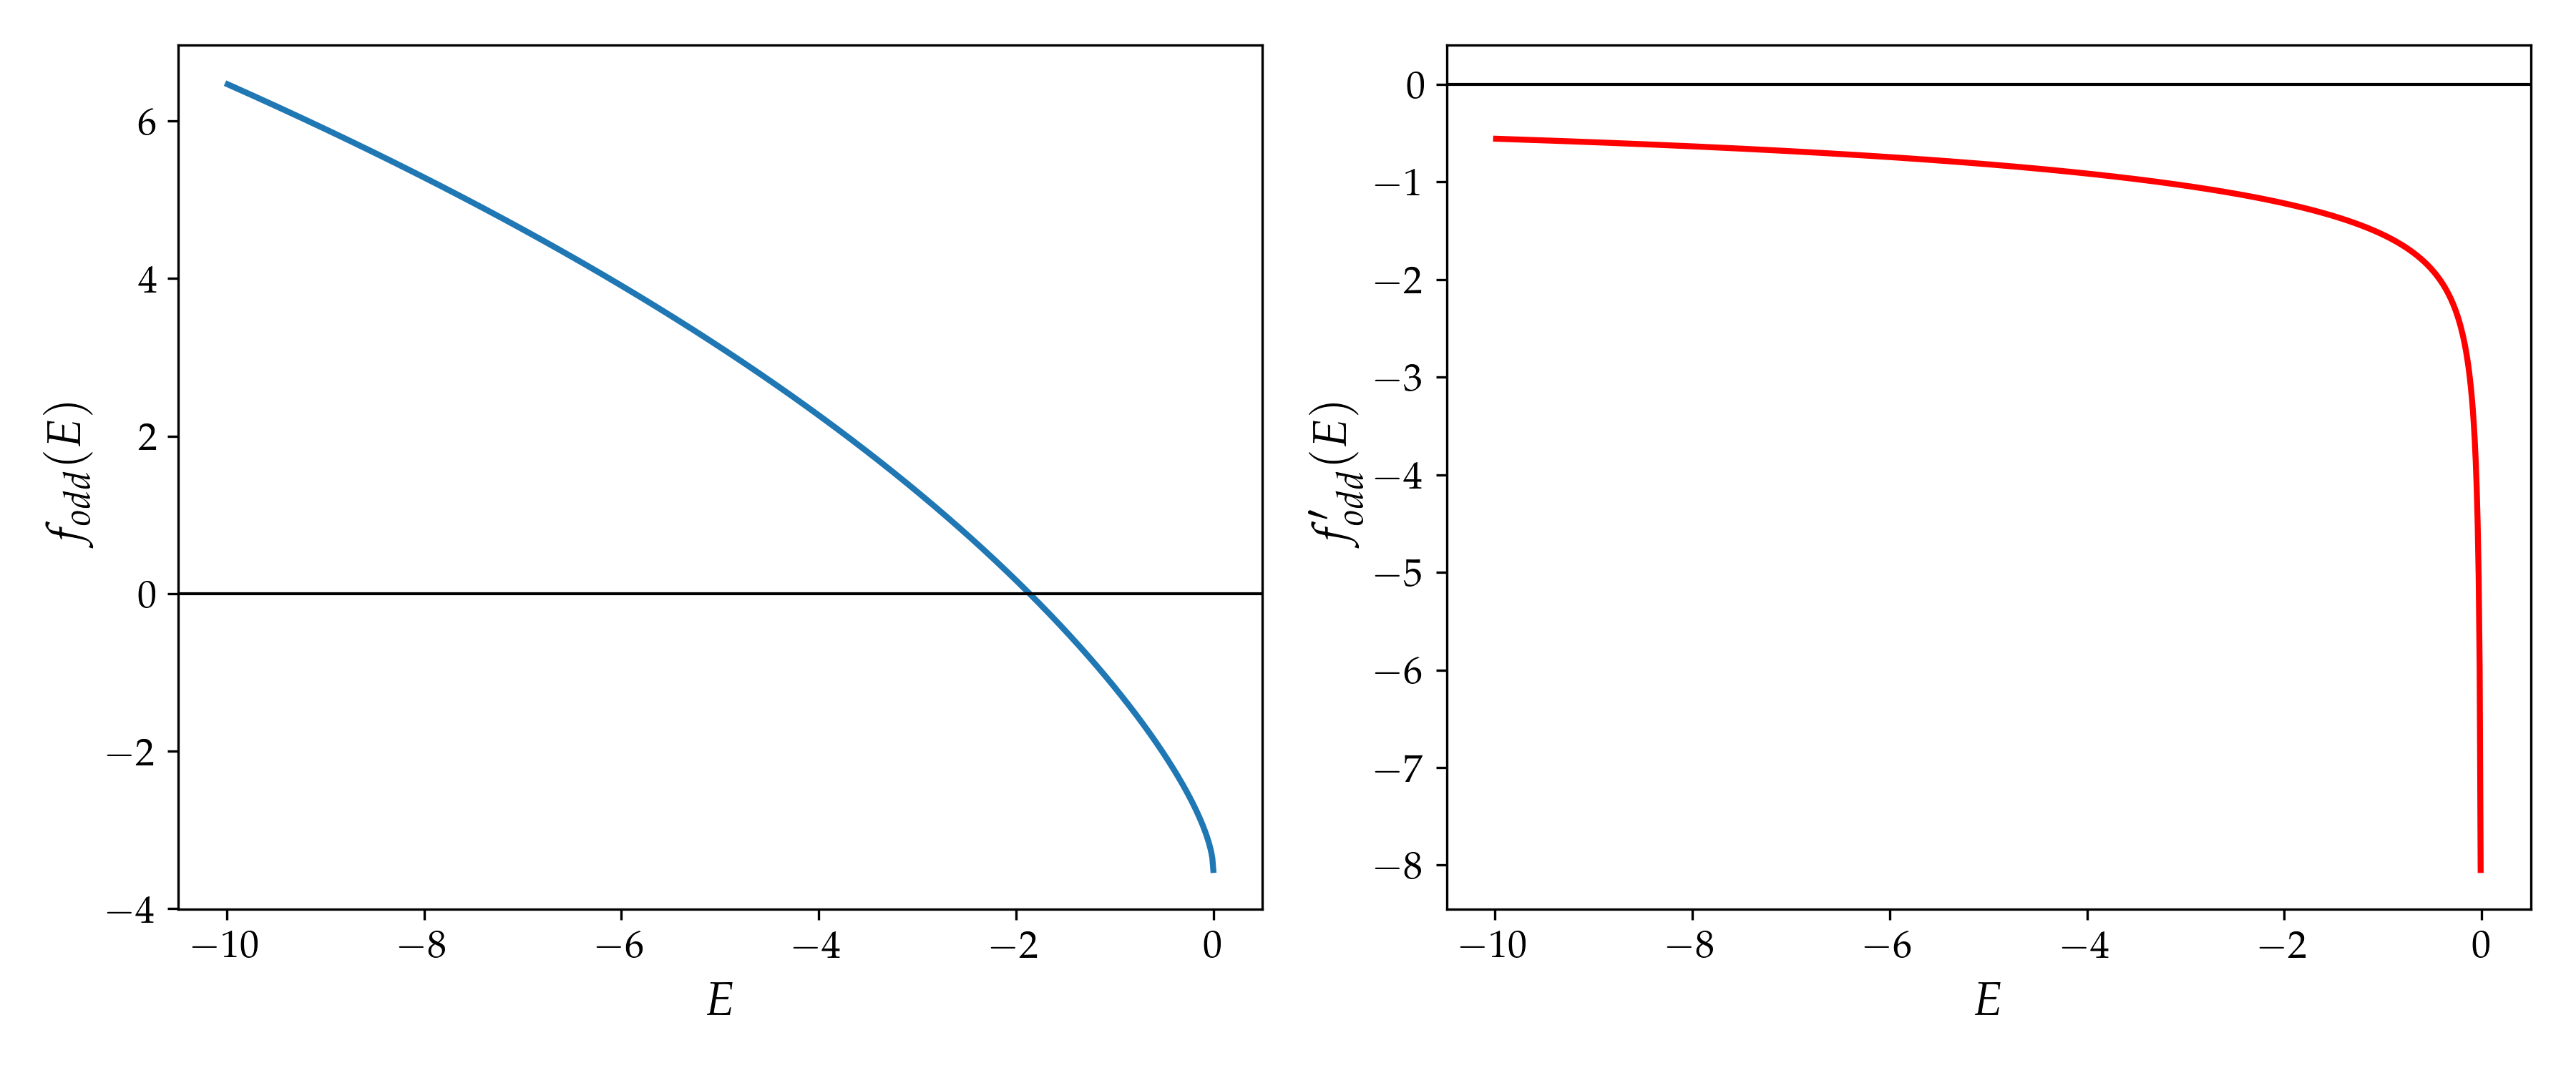
\includegraphics[width=\linewidth]{images/14/f_odd.png}
    \caption{Plot della funzione dispari e della sua derivata: nel dominio aperto mostrato non sono presenti singolarità e la funzione appare continua e derivabile.}
\end{figure}

I diversi metodi restituiscono i seguenti risultati:
\begin{elegantcode}
Bisection        c = -1.8628522388353397
                 iters = 46

Regula Falsi     c = -1.862852238835343
                 iters = 19

Secant           c = -1.86285223883534
                 iters = 6

Newton-Raphson   c = -1.8628522388353397
                 iters = 7
\end{elegantcode}


\bigskip\noindent Diamo quindi l'ultima descrizione del problema presentando i risultati finali per le due energie riferite agli stati legati con parità opposta, scegliendo come valori di riferimento numerici rispettivamente i due calcolati con il metodo di Newton-Raphson:
\begin{align*}
E_{\text{pari}} &= -7.705009250739082\\
E_{\text{dispari}} &= -1.8628522388353397
\end{align*}

\begin{figure}[H]
    \centering
    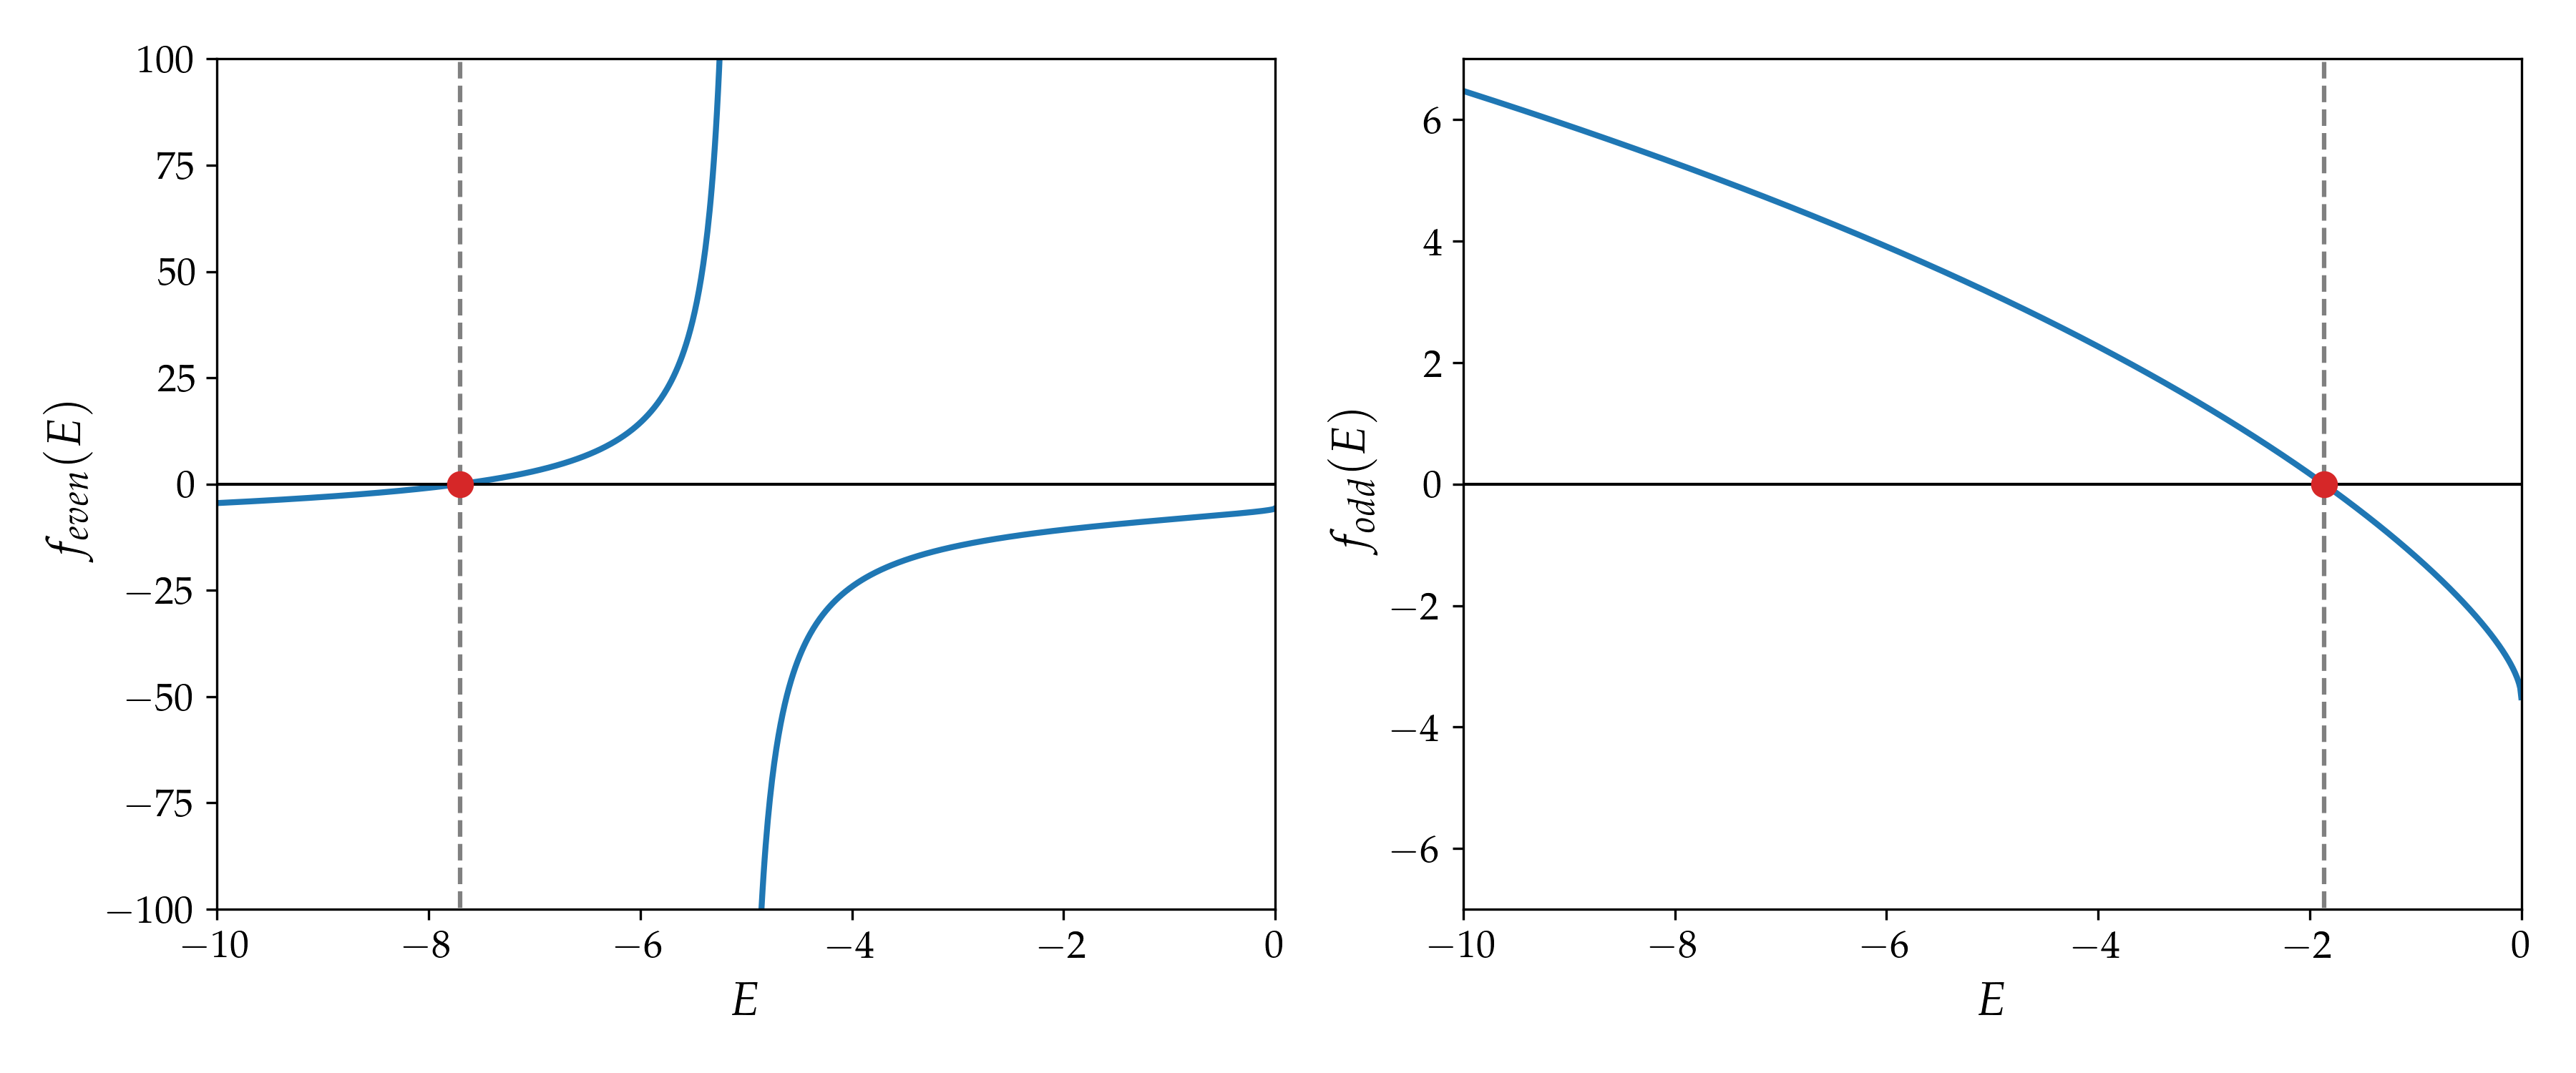
\includegraphics[width=\linewidth]{images/14/tot_f_plot.png}
    \caption{Rappresentazione delle due funzioni e degli zeri individuati con metodo di N-R.}
    \label{fig:placeholder}
\end{figure}


\newpage


\section{Esercizio 5.4.1}
\subsection{Problem Statement}

Scrivi un programma che, dato un polinomio, trovi le sue radici utilizzando la ricerca di autovalori discusso nella Sezione \textit{Problemi agli autovalori} e ne verifichi la correttezza. Si noti che il polinomio è completamente specificato dai coefficienti nella base monomiale. Scrivi il metodo di ricerca delle radici in modo modulare e applicalo ai seguenti casi:

\begin{enumerate}
    \item Il polinomio di Legendre di ordine 10
    \[
    \frac{1}{256}(46189x^{10} - 109395x^8 + 90090x^6 - 30030x^4 + 3465x^2 - 63)
    \]
    
    \item Il polinomio di Hermite di ordine 6
    \[
    H_6(x) = 64x^6 - 480x^4 + 720x^2 - 120
    \]
    
    \item I polinomi di Hermite soddisfano la relazione ricorsiva
    \[
    H_{n+1}(x) = 2xH_n(x) - 2nH_{n-1}(x), \quad H_0(x) = 1, H_{-1}(x) = 0
    \]
    Scrivi un programma che calcoli le radici del polinomio di Hermite di ordine $n$, $H_n(x)$. Costruisci il polinomio dalla relazione ricorsiva e verifica il risultato rispetto al compito precedente.
\end{enumerate}

Utilizza il risolutore di autovalori basato sulla decomposizione QR per questo esercizio.


\subsection{Premessa Teorica}
N-R si configura come un buon metodo, ma per il caso di una funzione con più radici esiste la possibilità che l'algoritmo converga su una  radice diversa da quella di nostro interesse. In più sarebbe interessante pensare di implementare un metodo che non debba ricercare i valori uno alla volta. In particolare ci occupiamo del caso in cui la funzione sia un polinomio di grado $n$, quindi con lo stesso numero di radici.\\

\medskip\noindent
Se definisco il polinomio
\[
    P_n(x) = c_0 + c_1 x + \dots + c_n x^n
\]

dividendo per $c_n$ e ridefinendo i $\bar c_i = c_i/c_n$:
\[
    P_n(x) = \bar c_0 + \bar c_1 x + \dots + x^n
\]

Introducendo la \textit{Companion matrix} $C_{ij}$:
\[
    C_{ij} = \begin{pmatrix} 
    0 & 1 & 0 & \dots & 0 & 0 \\
    0 & 0 & 1 & \dots & 0 & 0 \\
    \vdots & \vdots & \vdots & \vdots & \vdots & \vdots \\
    0 & 0 & 0 & \dots & 0 & 1\\
    -\bar c_0 & -\bar c_1 & -\bar c_2 & \dots & -\bar c_{n-2} & -\bar c_{n-1}
    \end{pmatrix}
\]

e il vettore $X_i(x) = (1,x,x^2 \dots x^{n-1})$, allora si può scrivere che:

\[
    \sum_j C_{ij} X_j(x) = \begin{pmatrix} x \\ x^2 \\ \cdots \\ -\bar c_0  -\bar c_1 x + \dots \end{pmatrix} = \begin{pmatrix} x \\ x^2 \\ \cdots \\ x^n - P_n(x) \end{pmatrix}
\]

Assumendo $P_n(x_0)=0$, cioè $x_0$ una radice del polinomio:
\[
    \sum_j C_{ij} X_j(x_0) = x_0 \begin{pmatrix} 1 \\ x_0 \\ \cdots \\ x_0^{n-1} \end{pmatrix} = x_0 X_i(x_0)
\]

\noindent Cioè $x_0$ è un autovalore di $C_{ij}$, con autovettore $X_i(x_0)$: abbiamo quindi la possibilità di implementare gli algoritmi dei capitoli precedenti per la ricerca di questi autovalori, e usando per esempio il \textit{QR eigensolver} possiamo trovarli tutti in una sola volta. La base che formano questi autovettori rappresenta i vettori riga della matrice di Vandermonde.

\subsection{Metodi Numerici e Algoritmi}
\subsubsection{Polinomi di Legendre di ordine 10}
Le radici estratte sono:
\begin{elegantcode}
Roots Legendre 10: [-0.97390653 -0.86506337 -0.67940957 -0.43339539 -0.14887434  0.14887434
  0.43339539  0.67940957  0.86506337  0.97390653]
\end{elegantcode}

\begin{multicols}{2}
    \noindent e la loro rappresentazione grafica in Fig. \ref{fig: Leg10}. Già dalla figura si può vedere come le radici che troviamo siano una buona approssimazione di quelle reali, ma lo confermiamo con una valutazione della funzione in questi punti ($|\text{Leg}_{10}(x_i)|\approx0$); si noti che l'algoritmo QR, di cui facciamo uso, viene inizializzato ogni volta con uno shift random nel range $[0,1]$; lo shift casuale viene utilizzato per migliorare la convergenza del QR eigensolver ed evitare eventuali stagnazioni numeriche. Questo implica che i risultati esatti possono differire lievemente per ogni lancio del programma, così come il calcolo delle differenze che mostriamo qui di seguito: è indicativo soprattutto l'ordine di questi errori, che è molto piccolo, e comparabile con la \textit{machine precision} della precisione a 64 bit.
    \begin{elegantcode}
diff_0 = 5.68e-14
diff_1 = 1.04e-10
diff_2 = 3.73e-14
diff_3 = 2.62e-14
diff_4 = 1.72e-14
diff_5 = 1.90e-14
diff_6 = 4.30e-11
diff_7 = 2.93e-14
diff_8 = 4.48e-13
diff_9 = 6.25e-13
    \end{elegantcode}
        
\end{multicols}

\begin{figure}[H]
    \centering
    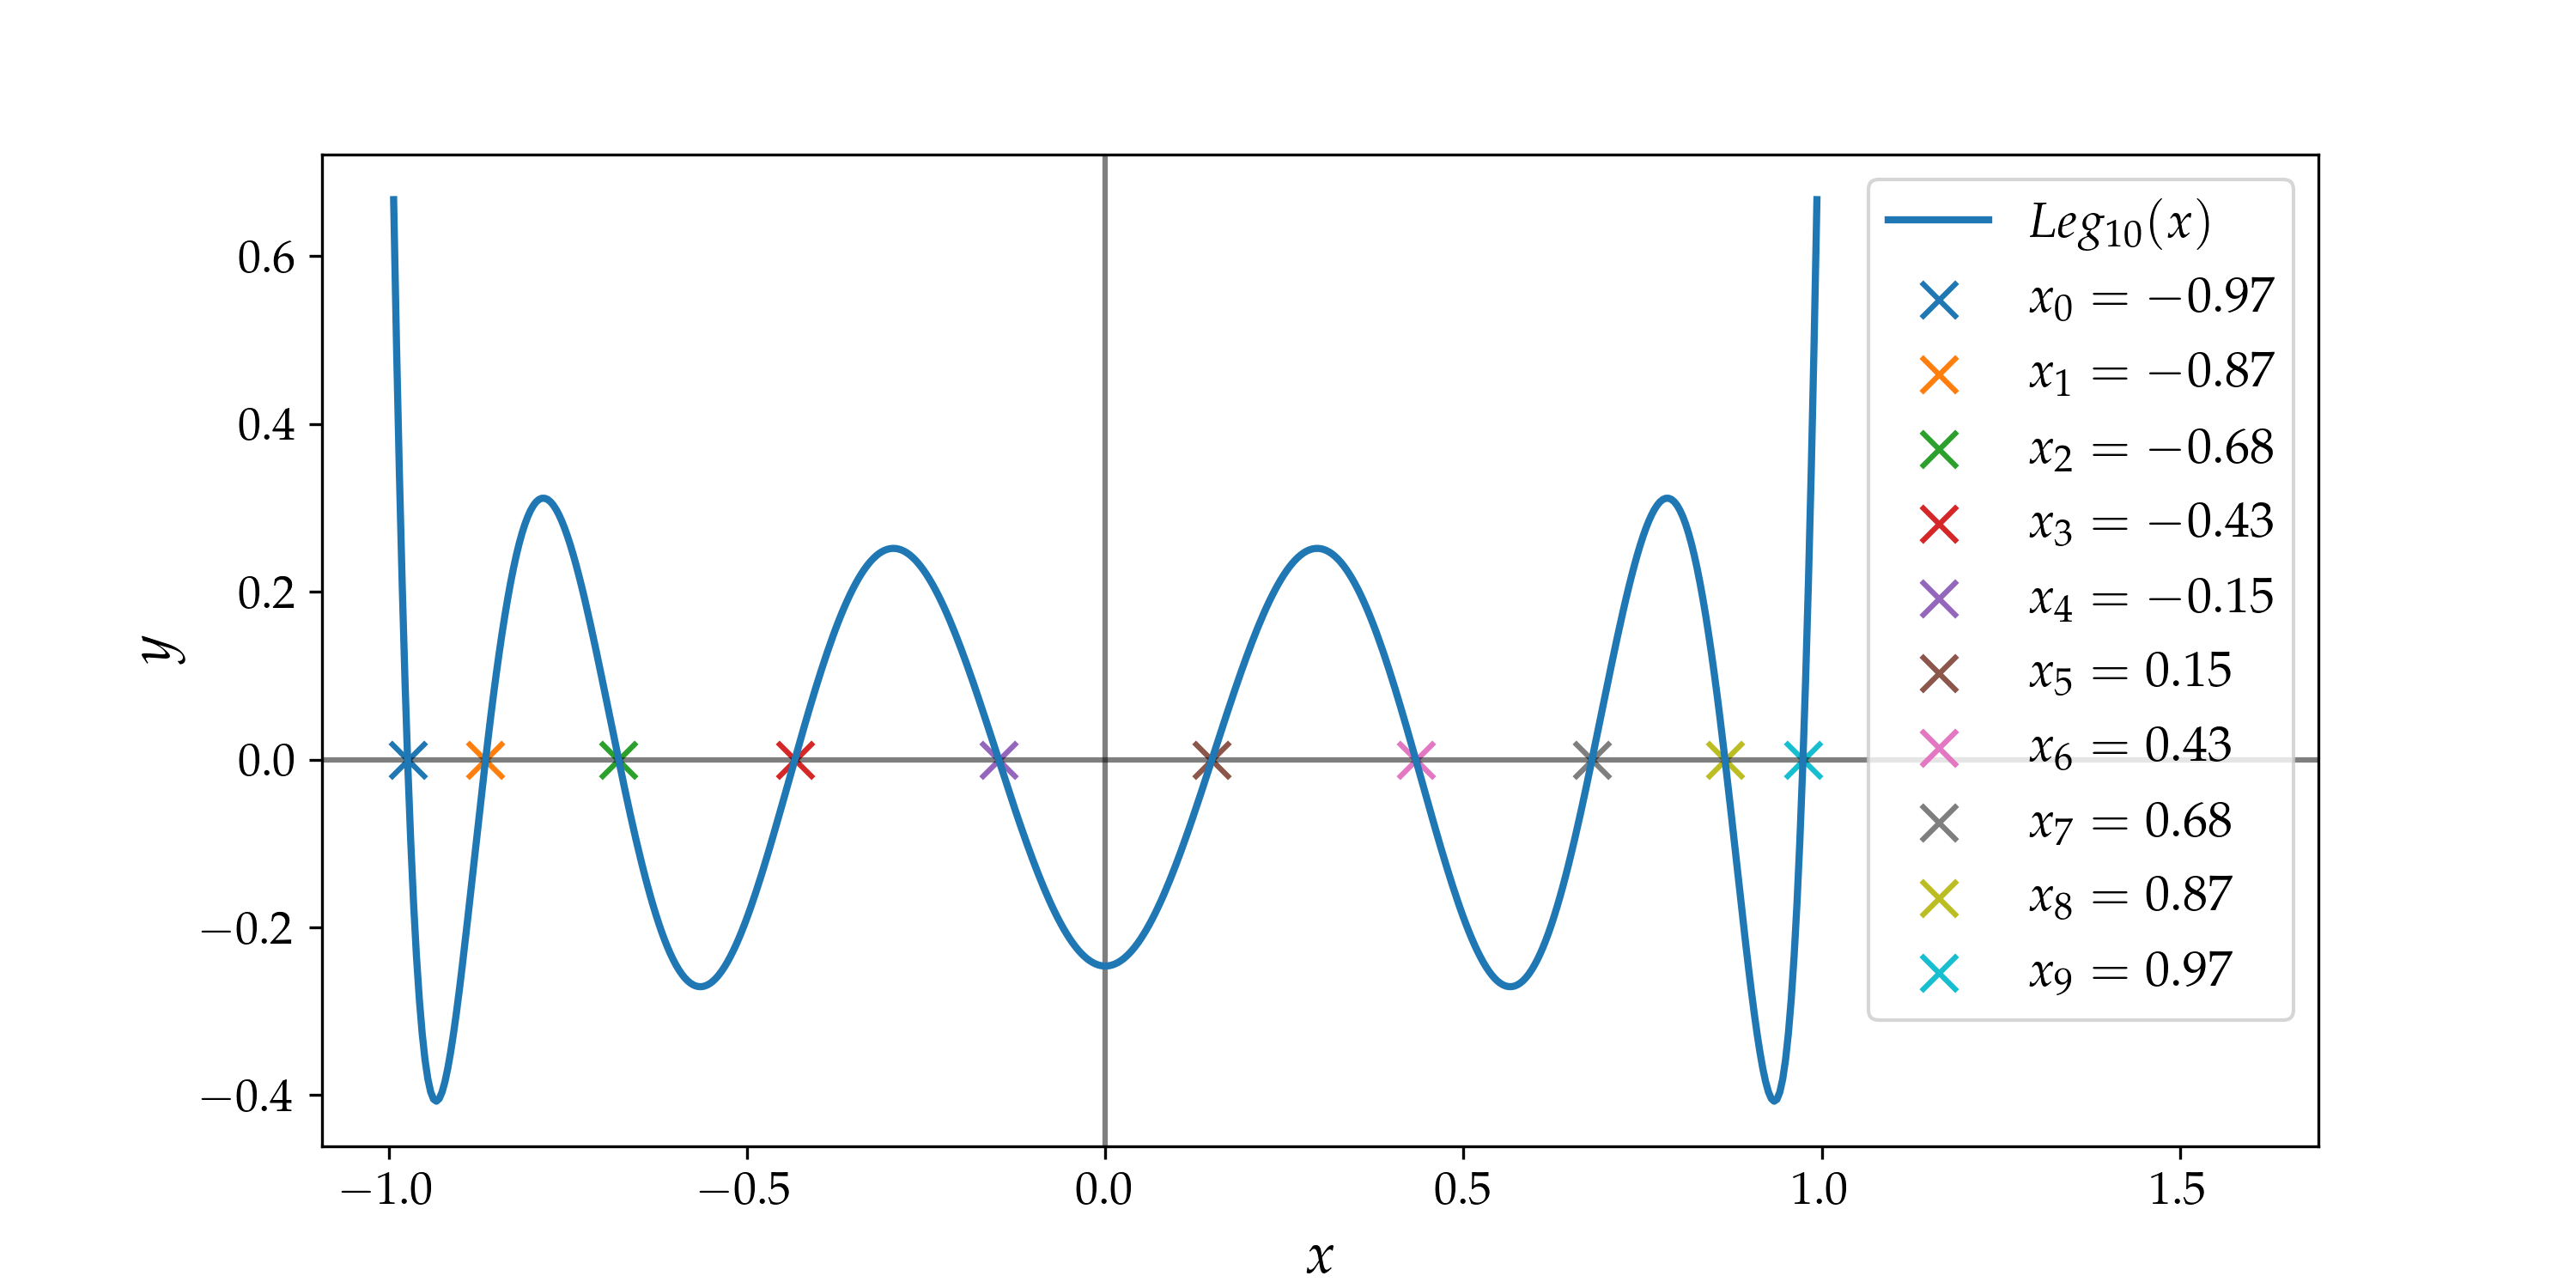
\includegraphics[width=0.8\linewidth]{images/15/Leg_root.png}
    \caption{Il polinomio $\text{Leg}_{10}(x)$, con le relative radici estratte dall'algoritmo.}
    \label{fig: Leg10}
\end{figure}


\subsubsection{Polinomi di Hermite di ordine 6}
Vale un discorso del tutto analogo per $\text{H}_6(x)$: i risultati di seguito.

\begin{elegantcode}
Roots Hermite 6: [-2.35060497 -1.33584907 -0.43607741  0.43607741  1.33584907  2.35060497]

diff_0 = 1.27e-10
diff_1 = 6.08e-12
diff_2 = 4.77e-15
diff_3 = 2.73e-12
diff_4 = 1.28e-11
diff_5 = 2.36e-11
\end{elegantcode}


\begin{figure}[H]
    \centering
    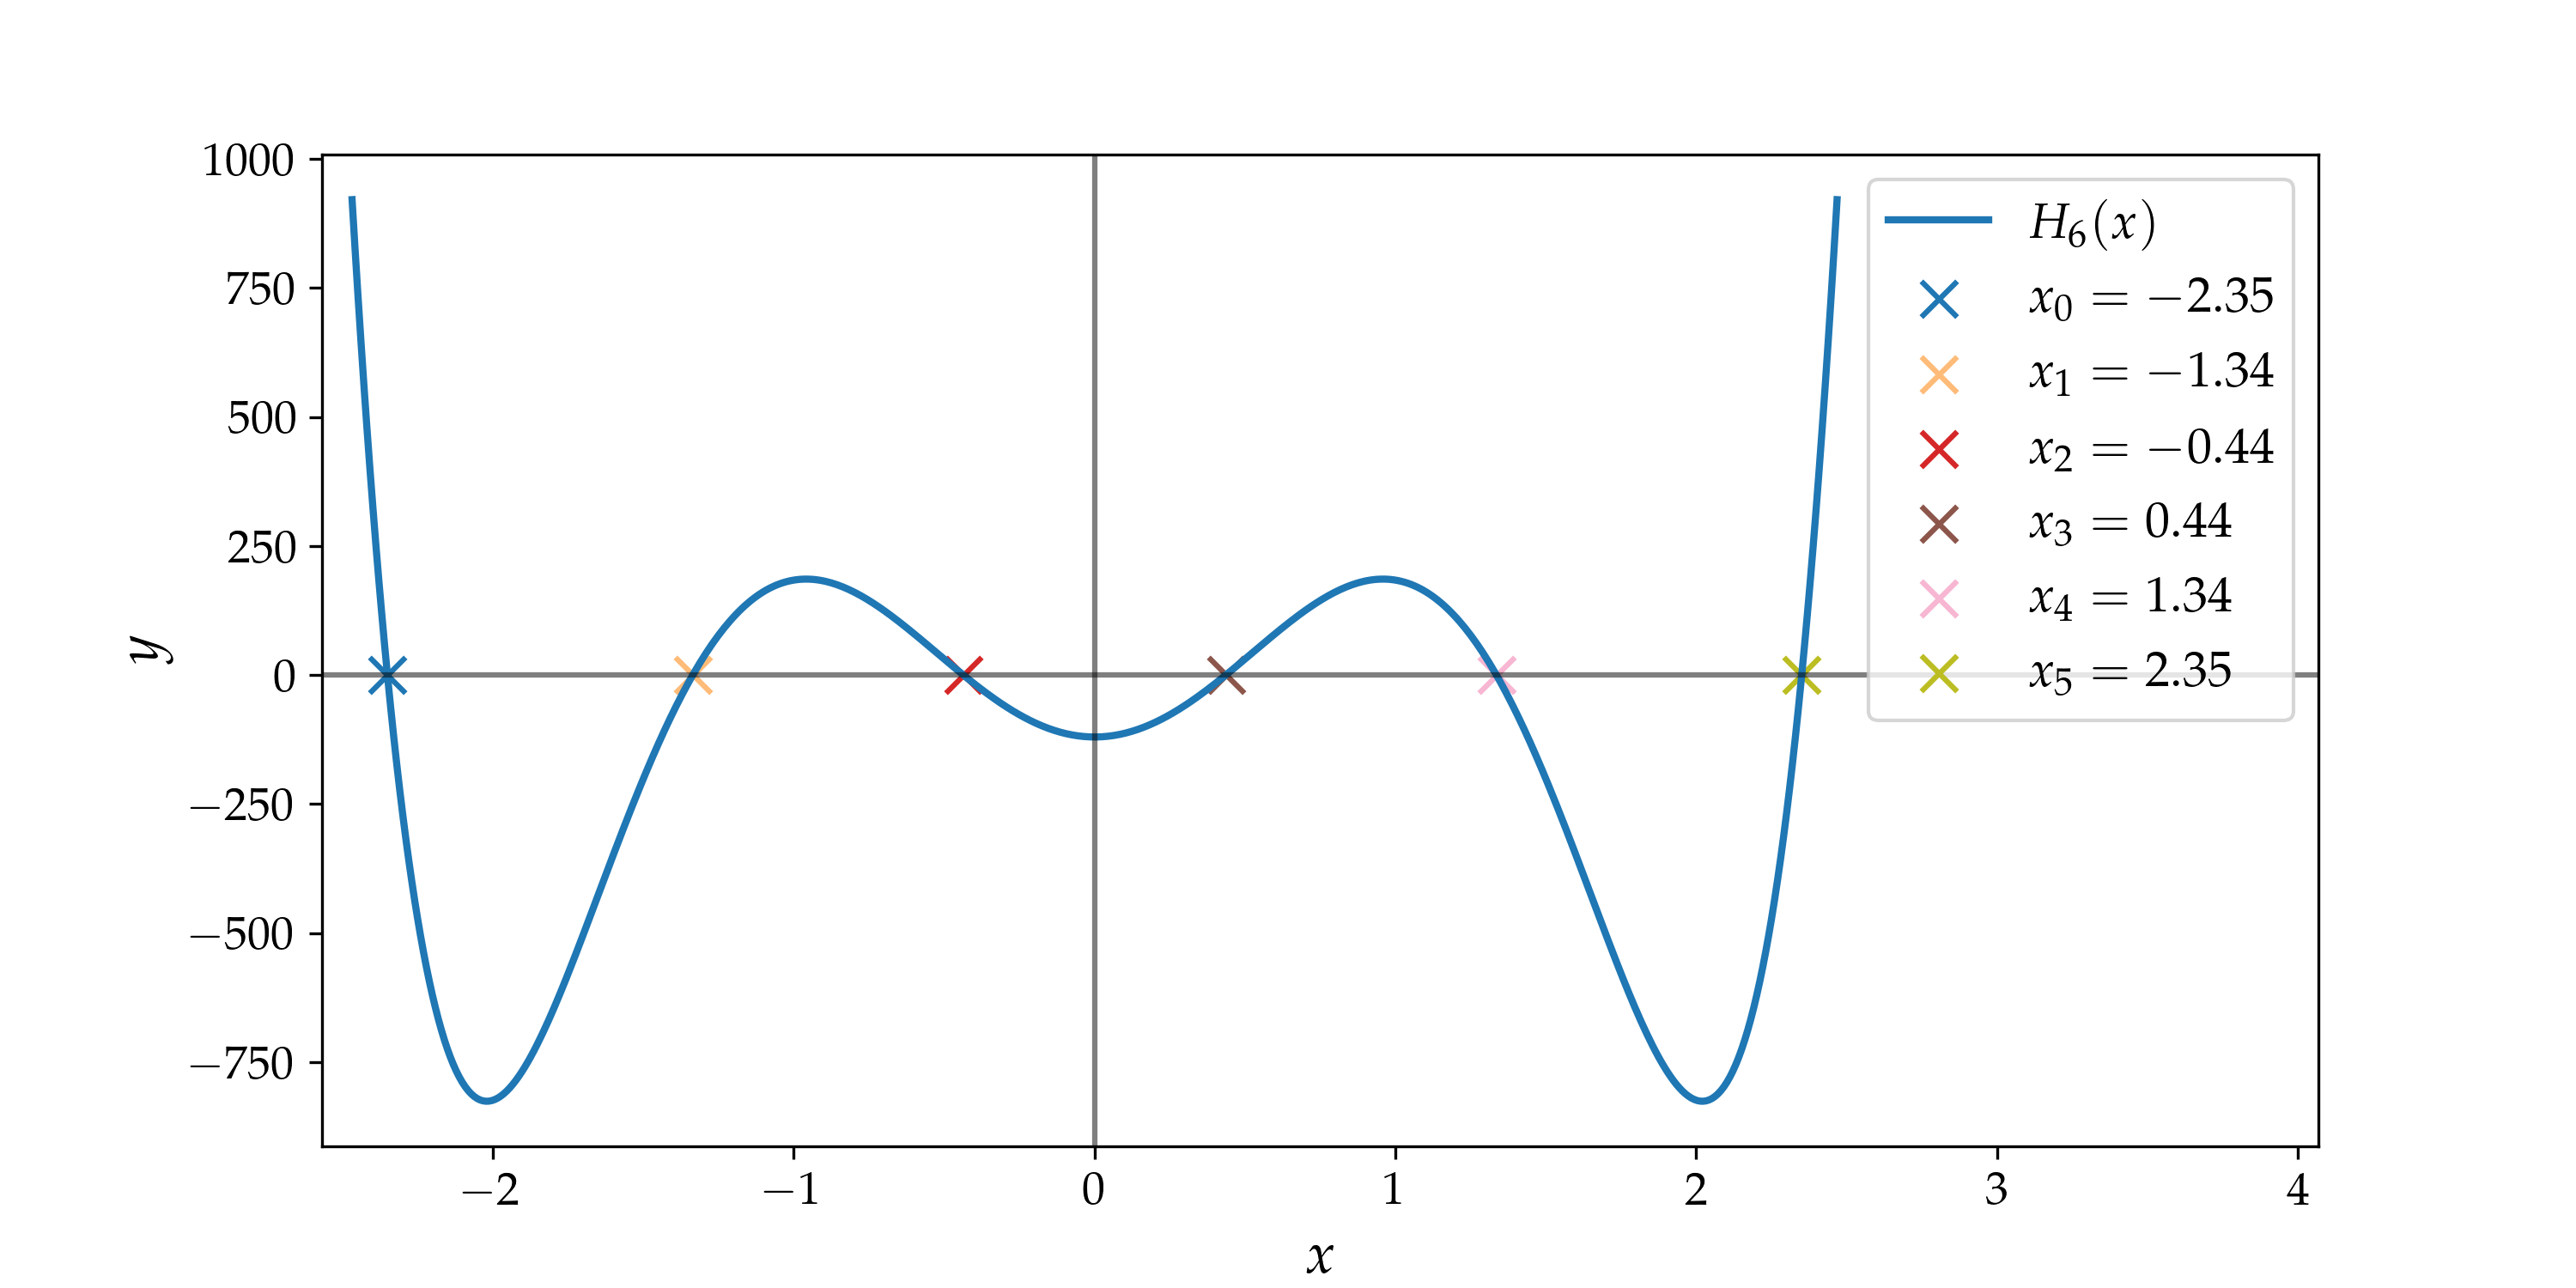
\includegraphics[width=0.8\linewidth]{images/15/Her_root.png}
    \caption{Il polinomio $\text{H}_{6}(x)$, con le relative radici estratte dall'algoritmo.}
    \label{fig: Her6}
\end{figure}


\subsubsection{Polinomi di Hermite di ordine n}
È stato implementato il metodo per il calcolo dei coefficienti del polinomio di Hermite di ordine $n$, che di conseguenza generalizza il caso precedente: siamo quindi interessati a confermare i risultati con un confronto tra i due metodi, che dovrebbero, chiaramente, essere interscambiabili.

\medskip\noindent
In particolare valutiamo la metrica
\[
\delta = \sqrt{\sum_{i=0}^5 (\bar x_i - x_i)^2}
\]
definendo $\bar{\boldsymbol x}$ come il vettore delle radici trovate con il metodo generalizzato.\\
Il risultato numerico è:
\[
\delta = 1.34\times 10^{-13}
\]
Il valore ottenuto è estremamente piccolo ed è compatibile con gli errori numerici accumulati durante il calcolo in precisione doppia.
\newpage








\newpage
% \thispagestyle{empty} 
\null 
\clearpage

% --- PARTE 6: Equazioni differenziali ordinarie (ODE) ---
\cleardoublepage 
\addtocontents{toc}{\bigskip\noindent\protect\textbf{\Large Equazioni differenziali ordinarie}\par\smallskip}
\addtocontents{toc}{\protect\setcounter{tocdepth}{-2}} 
\part{\Huge Equazioni differenziali ordinarie}
\addtocontents{toc}{\protect\setcounter{tocdepth}{2}} 




\section{Esercizio 6.3.1}

\subsection{Problem Statement}
Scrivere un programma che risolva un'equazione differenziale utilizzando il metodo RK2.
\noindent Testare il programma con l'equazione differenziale dell'oscillatore armonico con i seguenti valori iniziali:

\[
\ddot{\theta}(t) = -\theta, \quad \text{con } \theta(0) = 0 \text{ e } \dot{\theta}(0) = 1,
\]

\begin{itemize}
    \item Ottenere la soluzione analitica $\theta(t)$ e confrontarla con la soluzione numerica $\eta(t; h)$ ottenuta tramite i metodi RK2 ed Eulero.
    \item Tracciare i grafici di $\theta(t)$, $\dot{\theta}(t)$ e il diagramma dello spazio delle fasi $\dot{\theta}(\theta)$.
    \item Studiare l'errore $\mathcal{E}(t, h) = \eta(t, h) - \theta(t)$ in funzione del passo $h$ a un tempo $t$ fissato e dimostrare che i metodi hanno l'ordine di precisione atteso.
\end{itemize}


\subsection{Premessa Teorica}
In questa sezione decidiamo di analizzare alcuni problemi di risoluzione di \textit{ODE}. In generale definiamo:
\[
\frac{d y}{dx} = f(x, y(x)), \quad y(x_0) = y_0,
\]

come il problema al valore iniziale, del primo ordine. L'obiettivo è quindi determinare la funzione $y(x)$, conoscendo una condizione sulla derivata prima ($f$) e il valore della funzione in un punto $(y_0)$.

\subsection{Metodi Numerici e Algoritmi}
Si può definire un primo metodo approssimativo, che è quello di Eulero: dalla semplice riscrittura della parte sinistra dell'equazione usando le differenze finite, possiamo avere una prima via di risoluzione, con un algoritmo iterativo.\\
In particolare il "Forward Euler Method"
\footnote{
Così denominato poiché fa uso della definizione \textit{forward} della differenza finita. Sarà quindi possibile definire anche un algoritmo \textit{backward}, ma con caratteristiche leggermente diverse e che non approfondiamo in questa sezione.
}
:
\[
    \eta(x+h, h) = \eta(x,h) + h f(x, \eta(x,h))
\]

dove abbiamo denominato $\eta(x+h, h)$ la soluzione numerica di della soluzione all'istante $x+h$: questa sarà in generale differente dalla soluzione vera $y(x)$.\\
Mantenendo la stessa notazione, ma passando ad un nuovo approccio, posso definire il metodo di Runge-Kutta di ordine 2 come:
\[
\eta(x+ h,h) = \eta(x,h) + h f\left(x + \frac{1}{2}h, \eta(x,h) + \frac{1}{2}hf(x, \eta(x,h))\right)
\]

L'interpretazione di quello che fa numericamente il metodo è da ritrovare nella sua solita denominazione di \textit{midpoint method}: per stimare il valore della funzione in $x+h$, conoscendo il suo valore in $x$, possiamo usare la pendenza in $x$. Approssimare la funzione ad una retta è una possibile approssimazione per uno step piccolo; la scelta di RK2 è di fare due valutazioni della funzione, una volta per stimare il valore nel punto intermedio, cioè a $x+h/2$, la seconda per fornire una stima più accurata della derivata al passo, che viene poi utilizzata nell’aggiornamento finale. Questo approccio è quello che differenzia Eulero e RK2, e che permette al secondo di migliorare notevolmente la sua accuratezza e stabilità.\\
Per entrambi i casi gli algoritmi sono iterativi: ad un passo n-esimo la soluzione numerica $\eta(x+ n h,h)$ è un'approssimazione di quella esatta $y(x + n h)$.

\medskip\noindent
Si può dimostrare che per il metodo di Eulero l'errore locale, cioè per la singola iterazione, con passo $h$, scala in modo quadratico. Per l'algoritmo RK2 vale la convergenza cubica.\\
In generale l'errore globale, che tiene conto dell'accumulazione degli errori ai passi n-esimi, è diverso da quello locale, solitamente maggiore: accade infatti che per questi due metodi la convergenza perda un ordine nello \textit{scaling}, perciò:
\begin{itemize}
    \item \textbf{Eulero}: scaling lineare.
    \item \textbf{RK2}: scaling quadratico.
\end{itemize}


\subsection{Risultati e Discussione}

L'oscillatore armonico è definito dall'equazione differenziale:
\[
\ddot\theta(t) +\omega^2 \theta(t) = 0
\]
La cui soluzione generale è:
\[
\theta(t) = A\cos(\omega t) + B\sin(\omega t)
\]

\noindent Nel nostro esercizio $\omega^2=1$, scegliamo $\omega=1$, e le condizioni al contorno determinano univocamente i parametri $A, B$:
\begin{align*}
    \begin{cases}
        \theta(0) = 0\\
        \dot \theta(0) = 1\\
    \end{cases}
    \quad \to \quad 
    A = 0, B= 1
\end{align*}

\[
\implies \theta(t) = \sin(t)
\]

L'idea è ora quella di confrontare il risultato analitico con quello numerico. In Fig. \ref{fig: rk2 th, dth} e \ref{fig: rk2 fasi} vediamo alcuni plot che riguardano il metodo RK2, diagrammi che mostrano il peso della scelta del passo nell'accuratezza della soluzione.\\
In Fig. \ref{fig: confr th,dth} e \ref{fig: confr fasi} i confronti sono fatti tra i due algoritmi di RK2 e Eulero, fissando un passo a $h=0.3$. 

\begin{figure}[H]
    \centering
    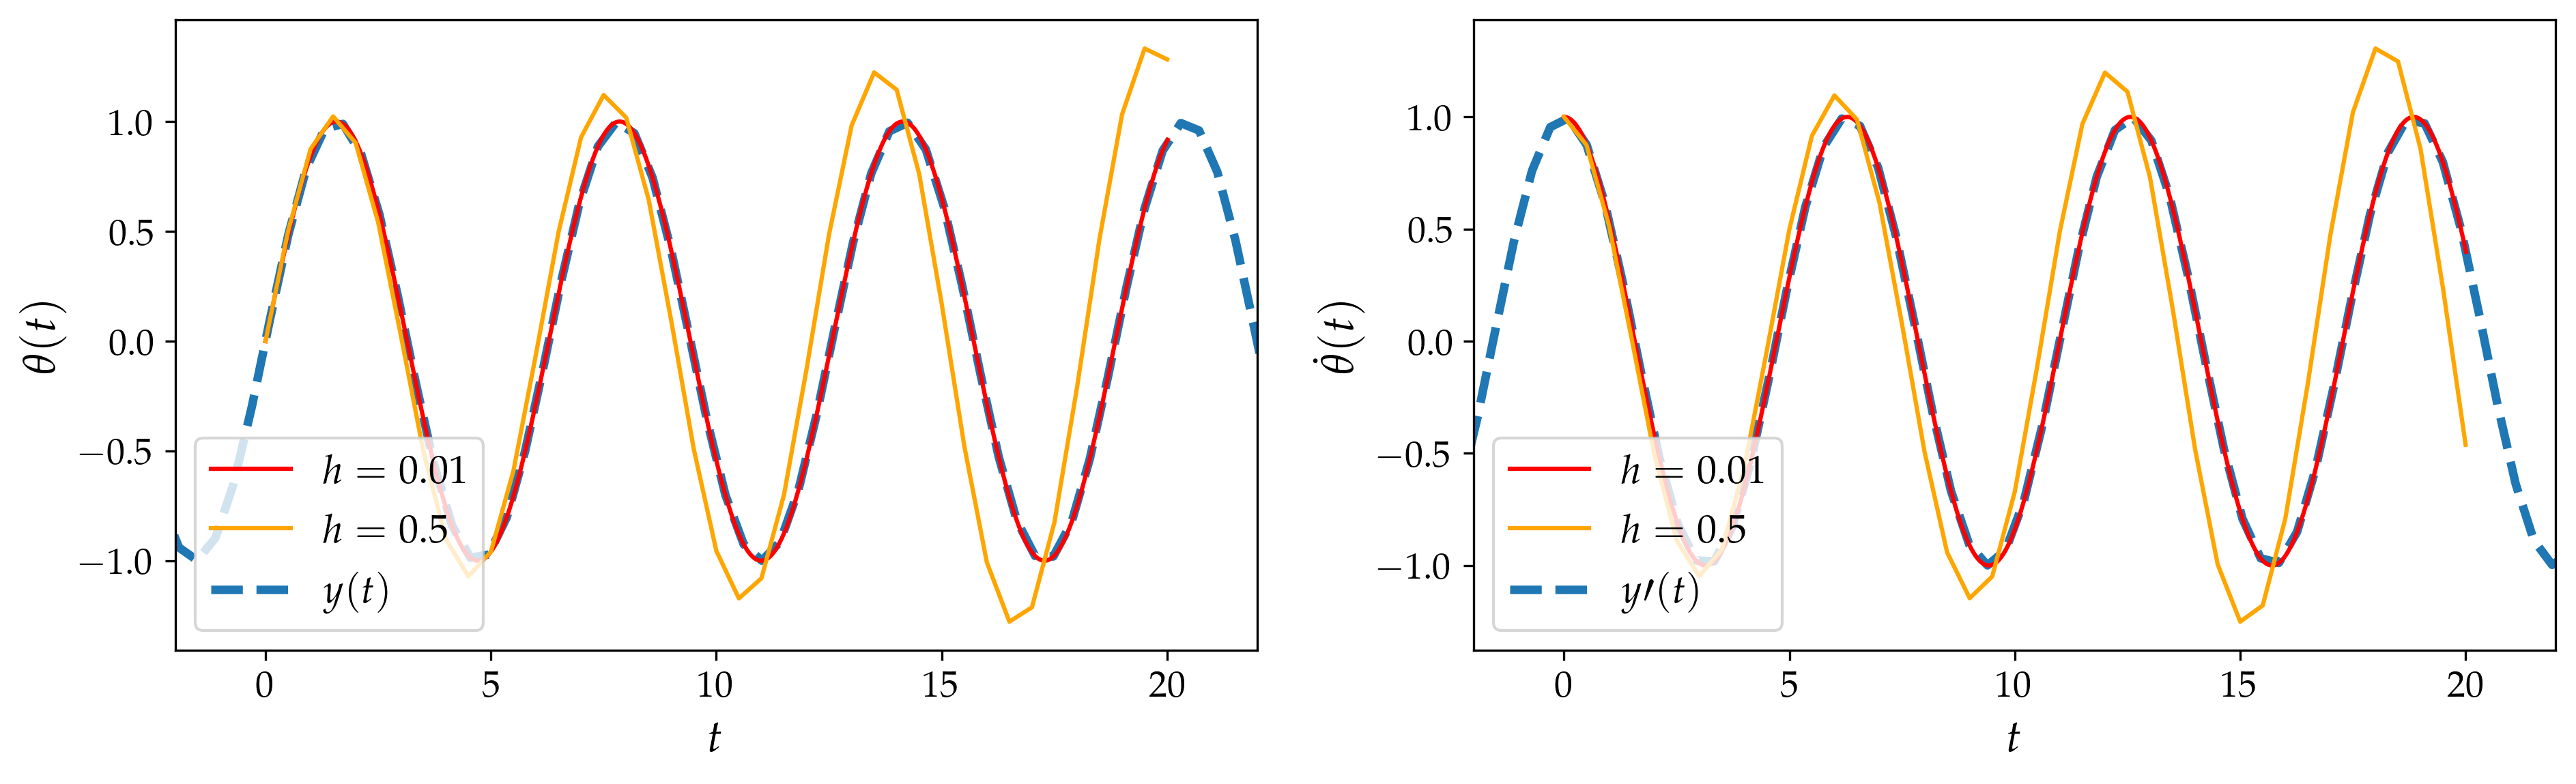
\includegraphics[width=\linewidth]{images/17/RK2_th_dth.png}
    \caption{In figura il plot che evidenzia come varia l'accuratezza del metodo RK2 con il passo, più grande o più piccolo. Come ci si aspetta, più piccolo il passo, migliore l'approssimazione di  $\eta(x+ n h,h)$ a $y(x + n h)$.}
    \label{fig: rk2 th, dth}
\end{figure}

\begin{figure}[H]
    \centering
    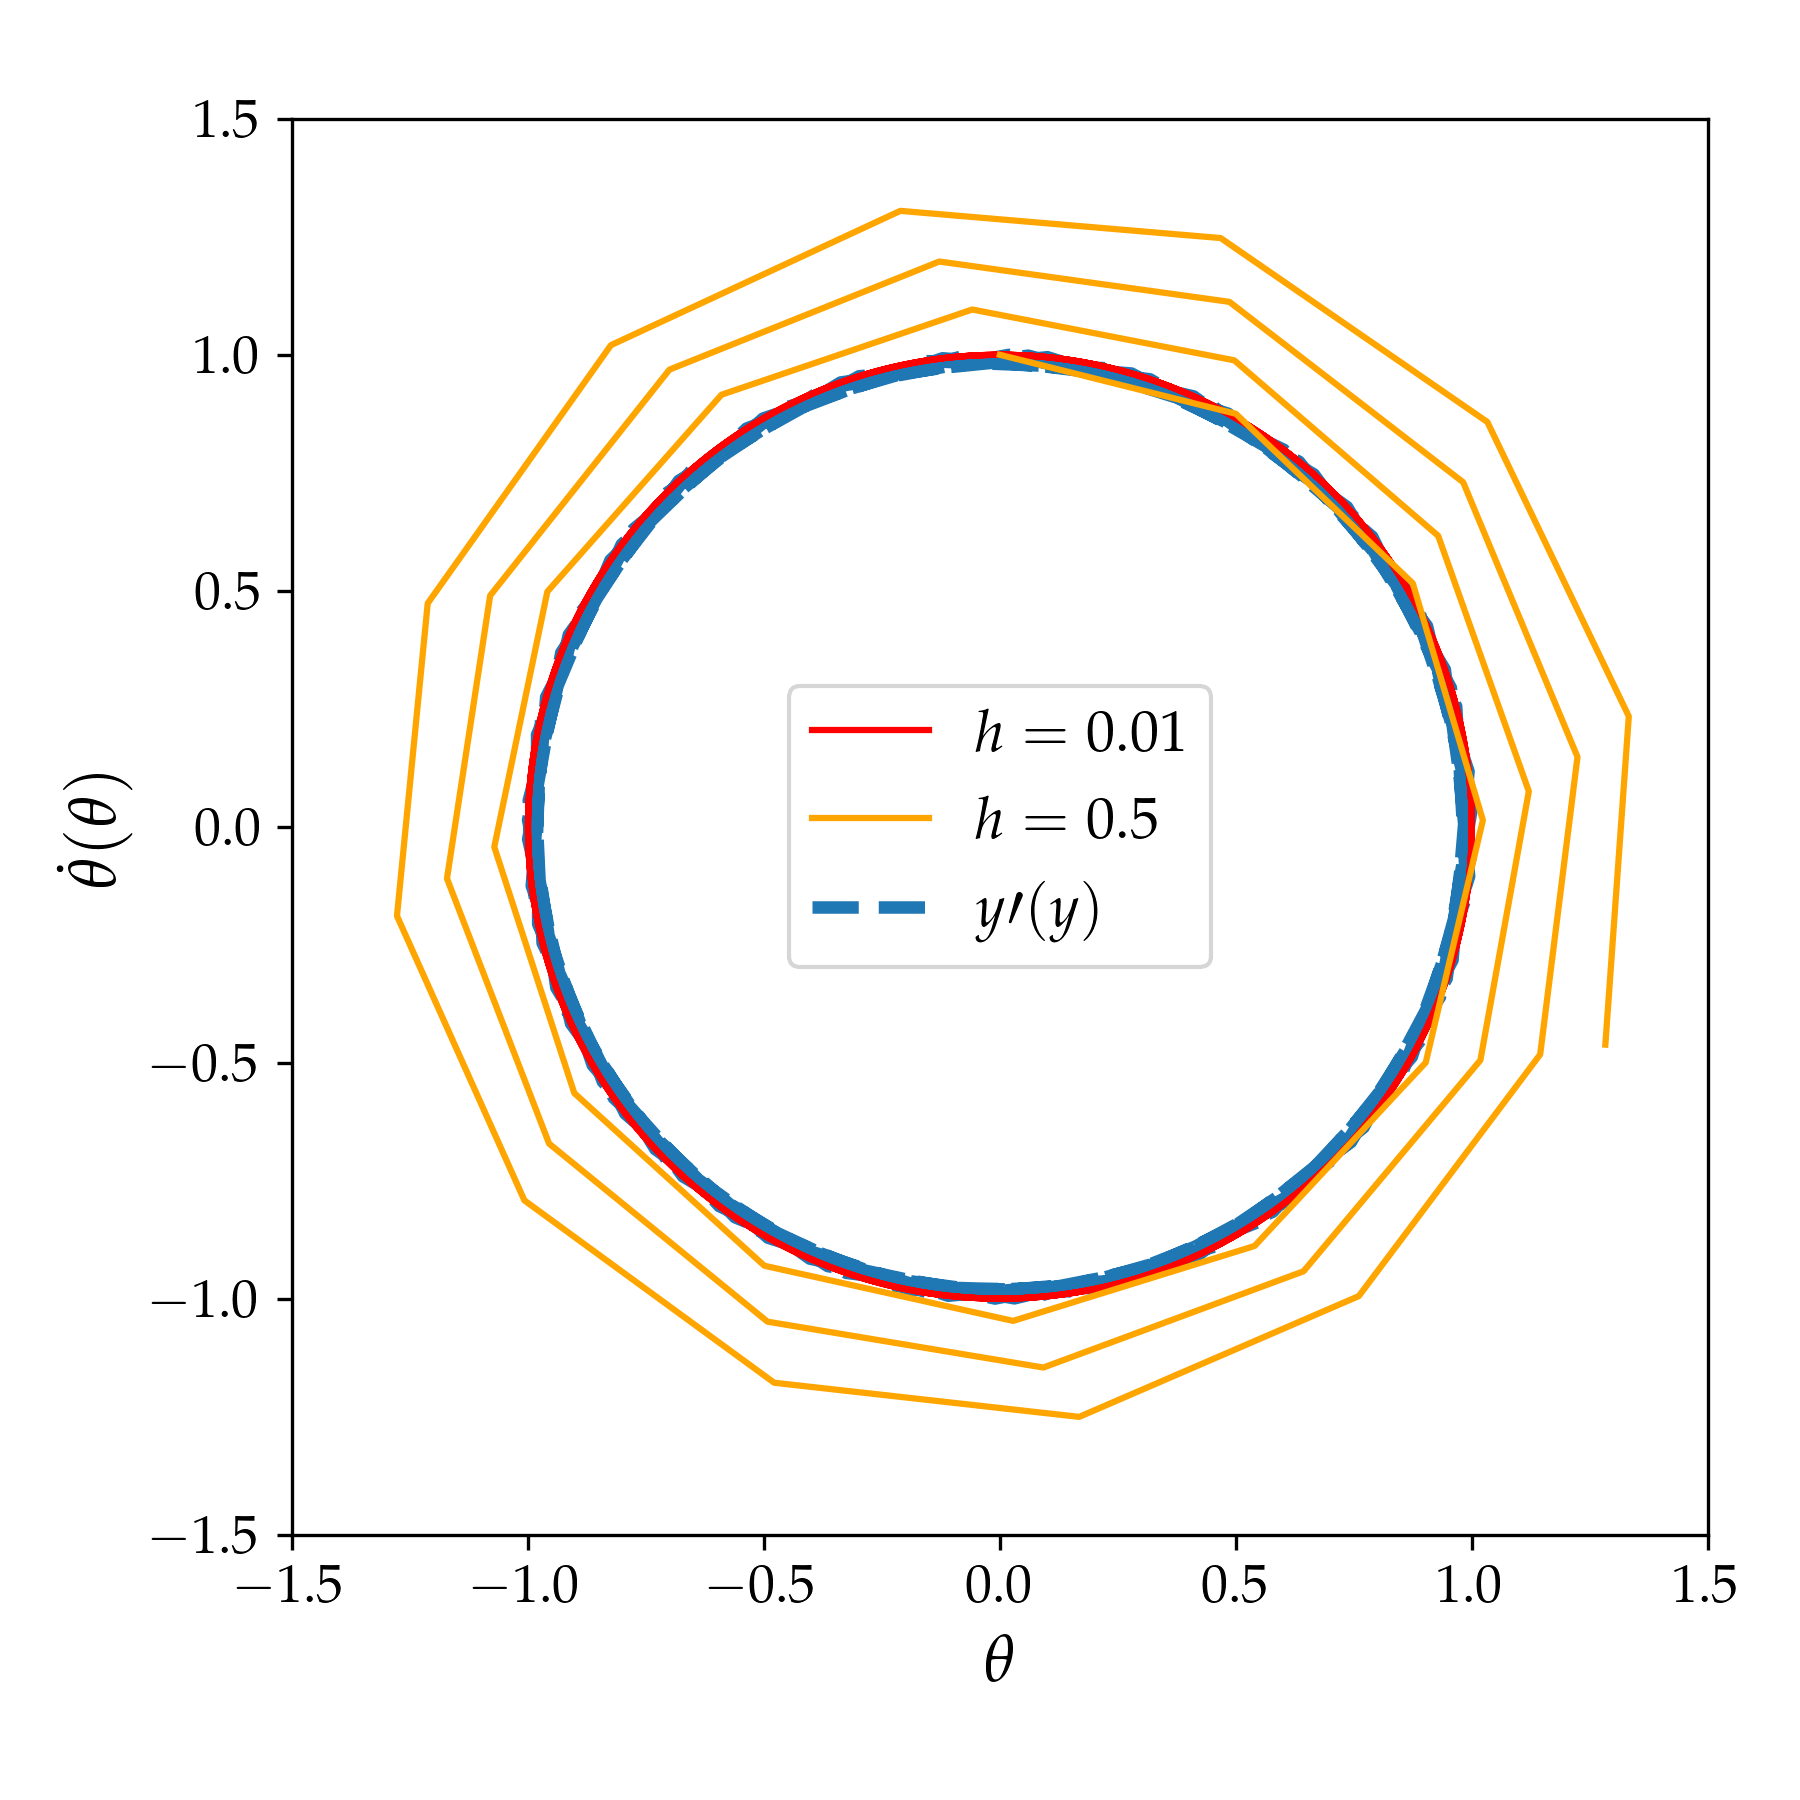
\includegraphics[width=0.6\linewidth]{images/17/RK2_fasi.png}
    \caption{Il diagramma delle fasi per RK2: si osserva un progressivo allontanamento dalla traiettoria esatta dovuto agli errori numerici accumulati, con passo di $h=0.5$, mentre l'approssimazione di $h=0.01$ è ottima nel confronto con la soluzione esatta.}
    \label{fig: rk2 fasi}
\end{figure}

\begin{figure}[H]
    \centering
    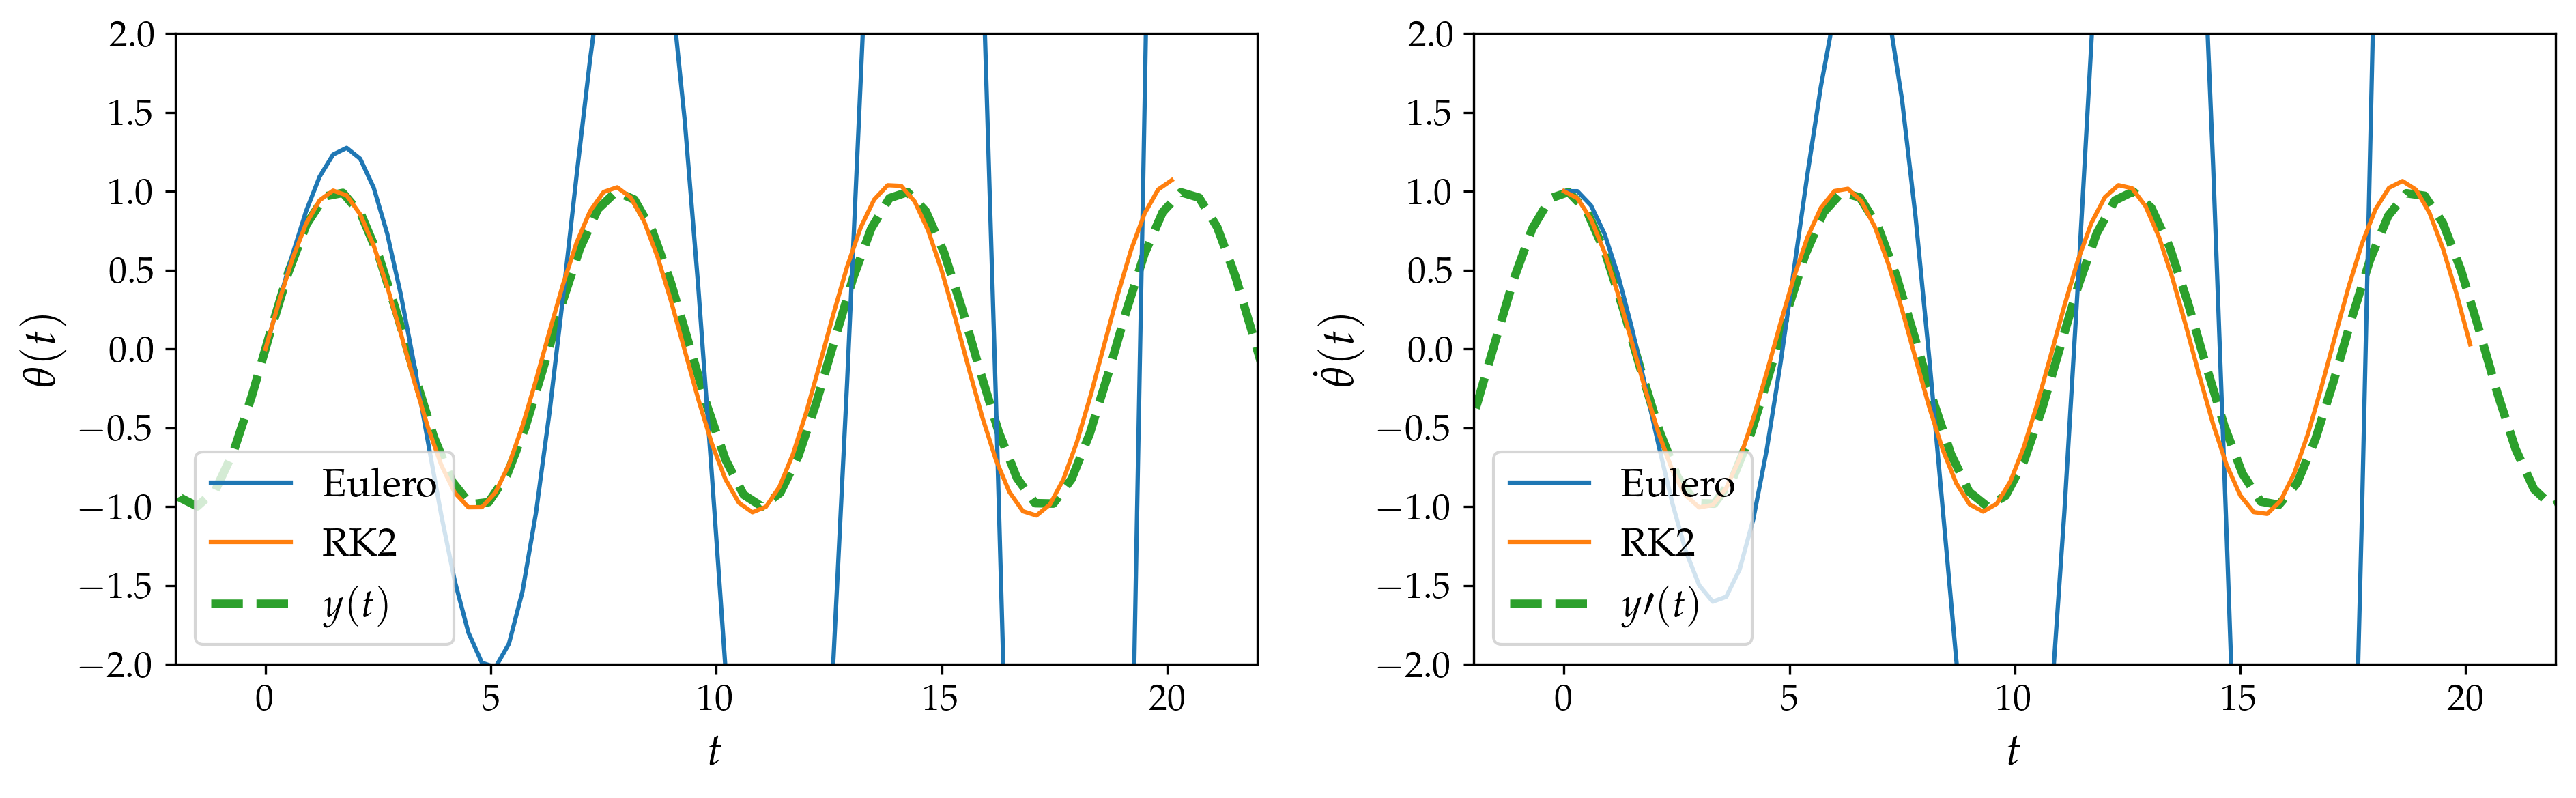
\includegraphics[width=\linewidth]{images/17/confr_th_dth.png}
    \caption{Le approssimazioni dei due metodi alla soluzione esatta: in entrambi è possibile apprezzare la maggiore stabilità della soluzione numerica di RK2, rispetto a quella di Eulero, che diverge velocemente.}
    \label{fig: confr th,dth}
\end{figure}


\begin{figure}[H]
    \centering
    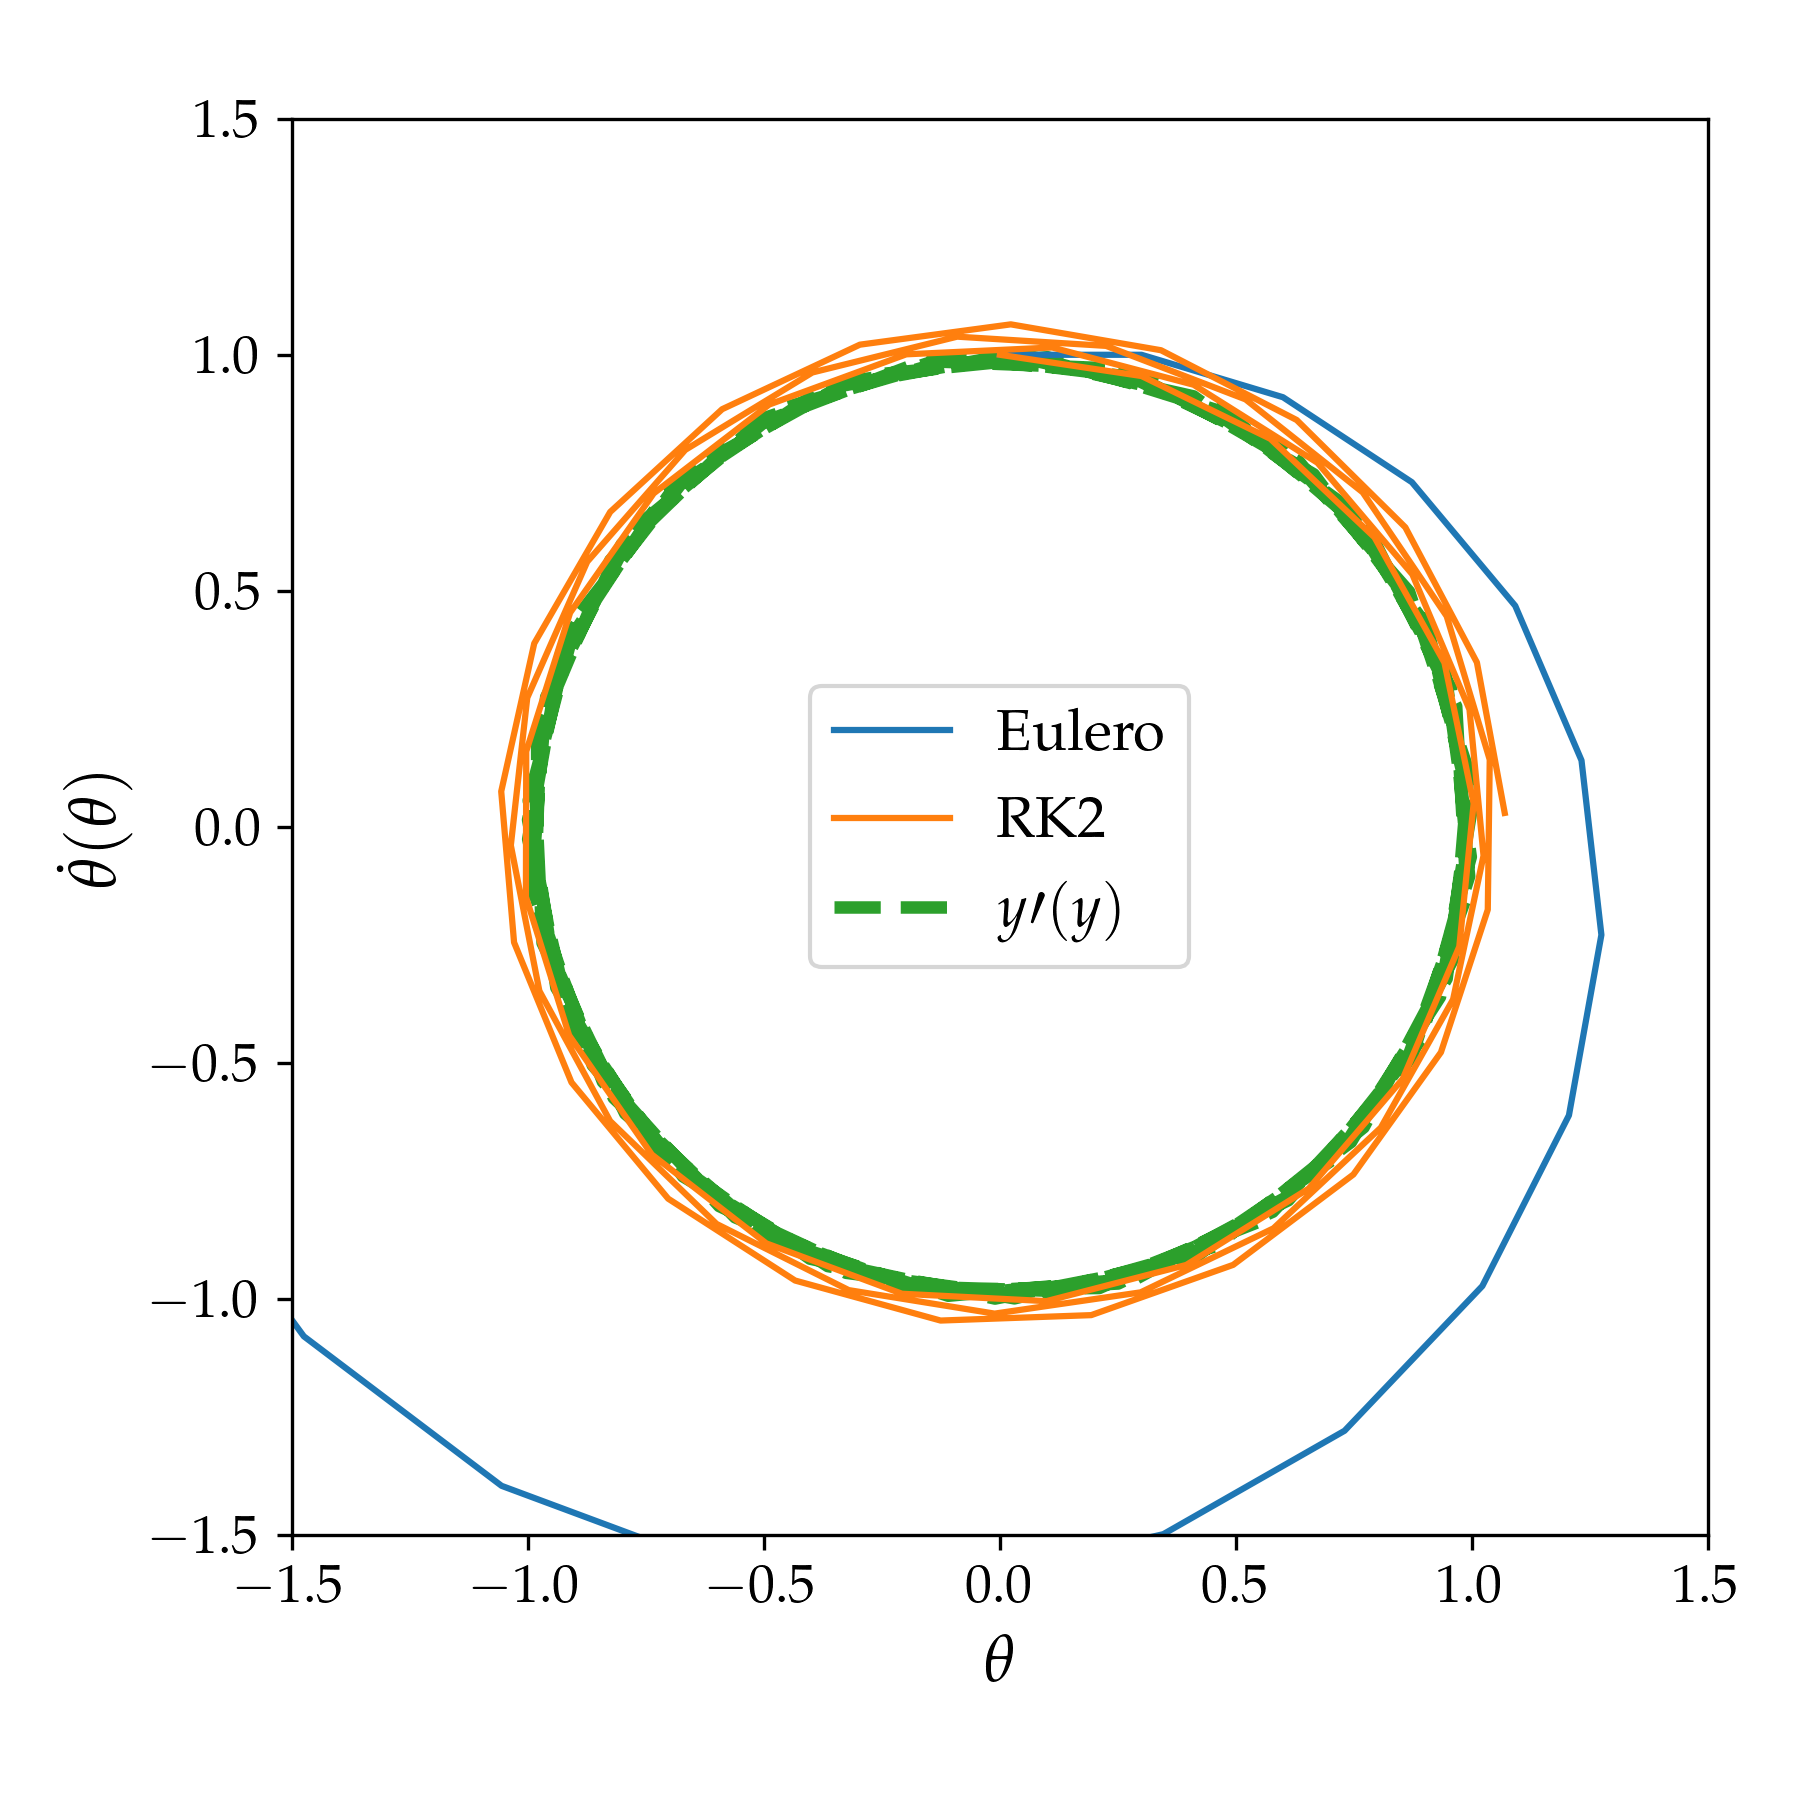
\includegraphics[width=0.6\linewidth]{images/17/confr_fasi.png}
    \caption{Il confronto tra i metodi viene esteso anche al diagramma delle fasi.}
    \label{fig: confr fasi}
\end{figure}

\noindent Lo studio dell'errore in funzione del passo $h$, ad un tempo fissato $t$ è in Fig. \ref{fig: Scaling confr}: definisco 
\[
\mathcal E(t, h) = \eta(t, h) - \theta(t)
\]
in particolare fissiamo il tempo $t=1$ e procediamo con l'analisi della convergenza dei metodi.

\begin{figure}[H]
    \centering
    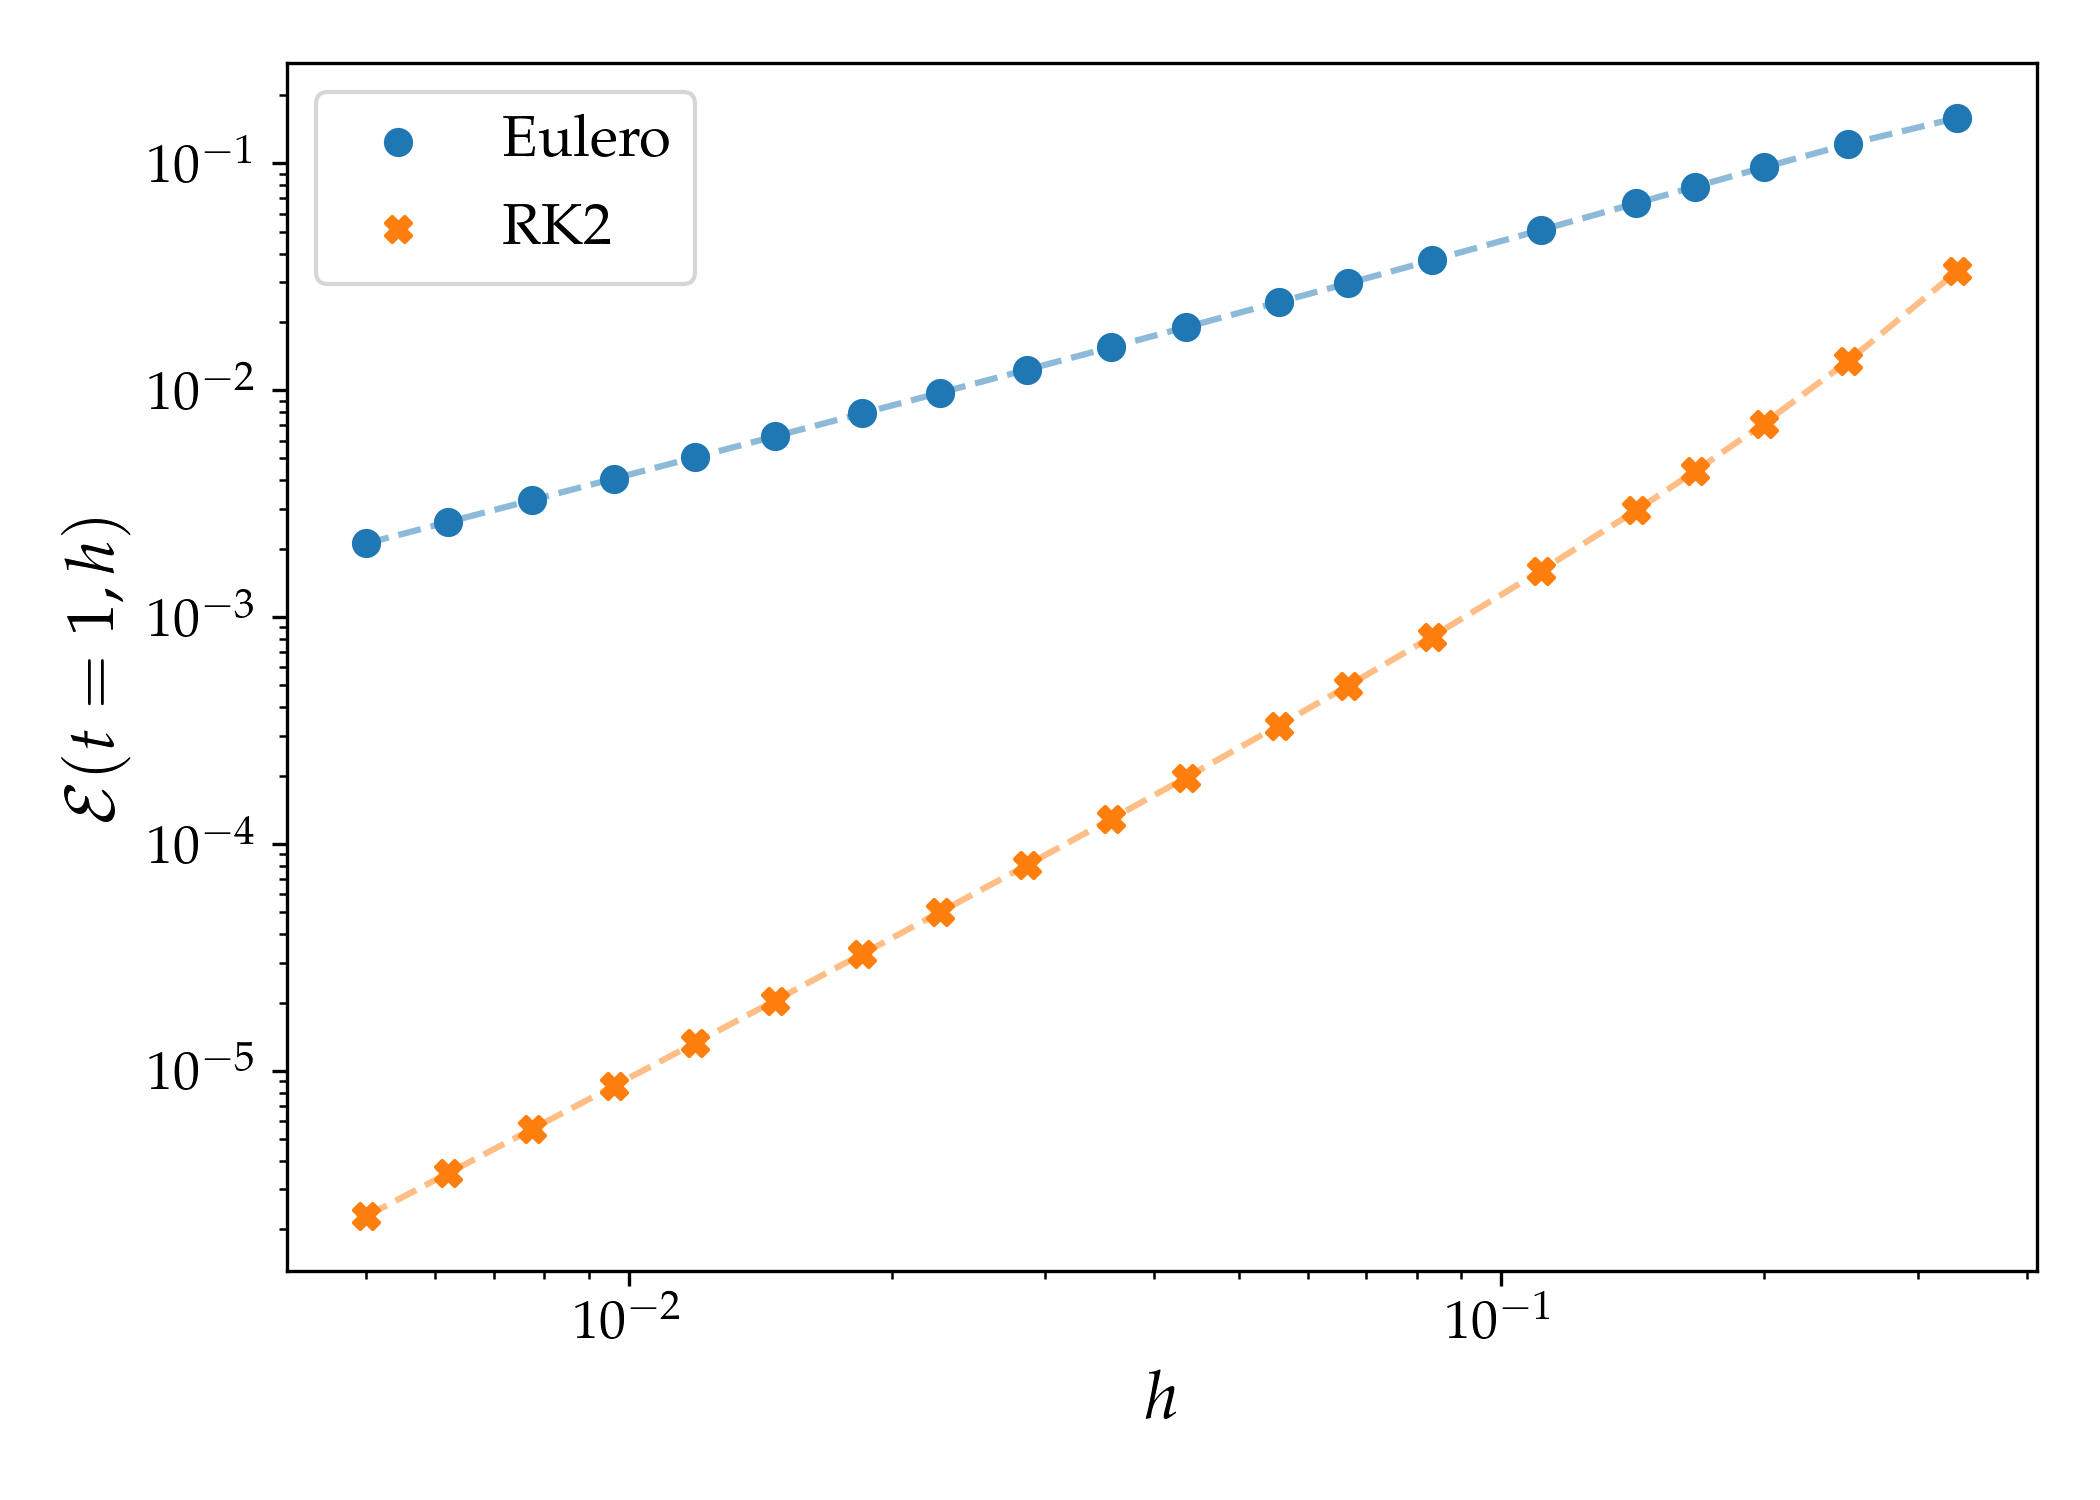
\includegraphics[width=0.7\linewidth]{images/17/scaling_confr.png}
    \caption{Confronto nello scaling dei singoli metodi. Si noti come la pendenza sia diversa, in particolare è maggiore per RK2: la sua convergenza è più rapida.}
    \label{fig: Scaling confr}
\end{figure}


\begin{figure}[H]
    \centering
    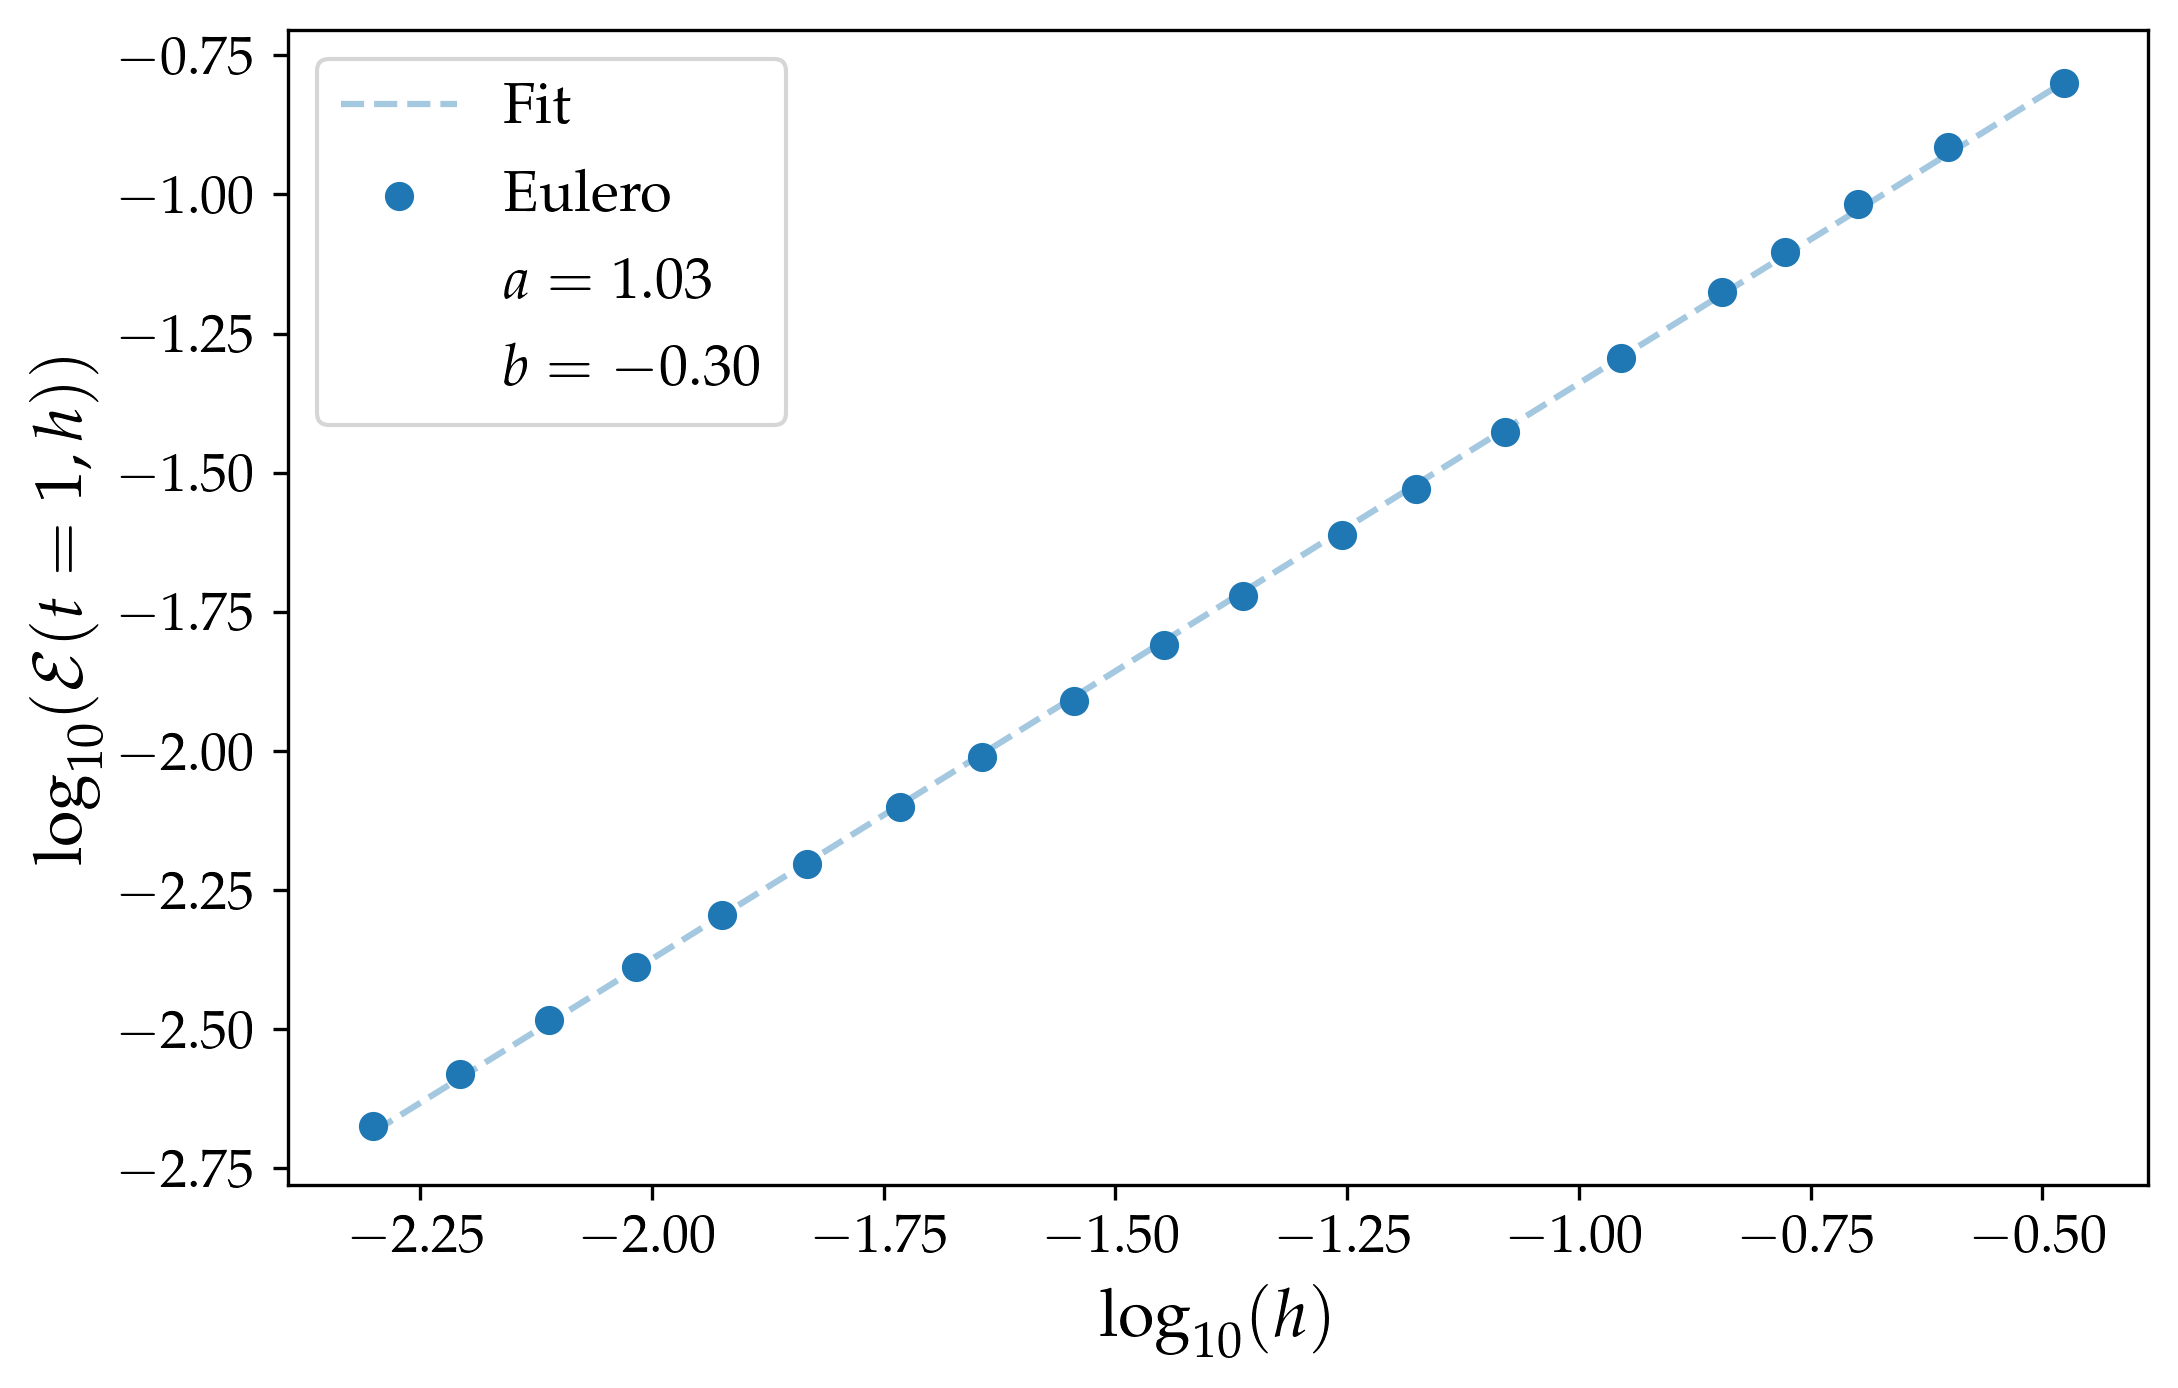
\includegraphics[width=0.8\linewidth]{images/17/fit_Eulero.png}
    \caption{Fit del metodo di Eulero: si verifica la convergenza lineare.}
    \label{fig: fit euler}
\end{figure}

\begin{figure}[H]
    \centering
    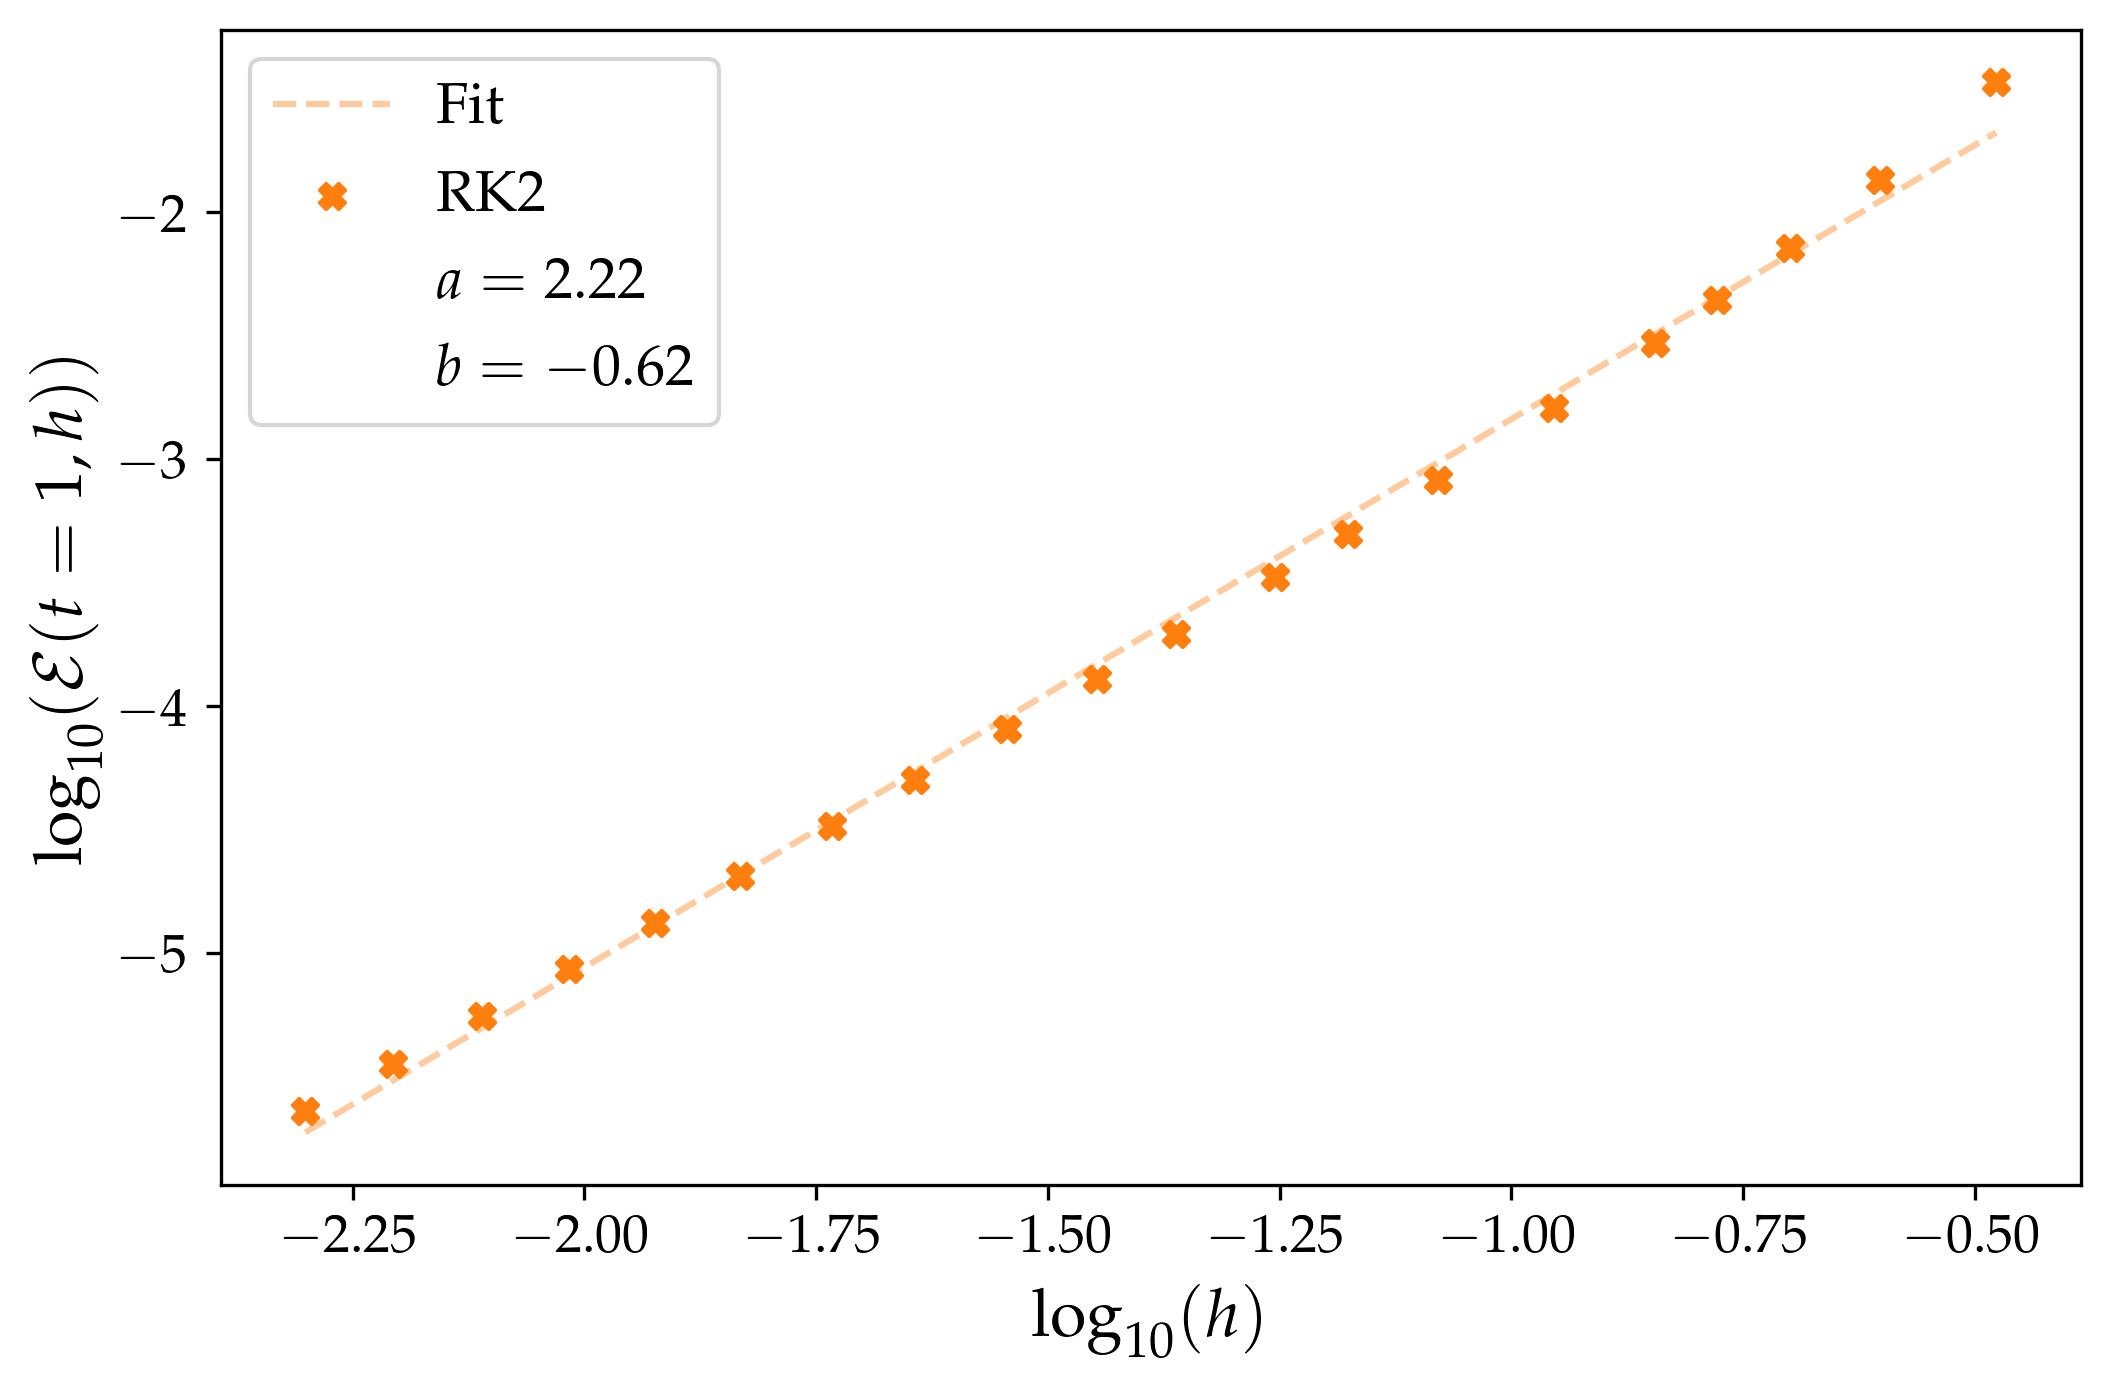
\includegraphics[width=0.8\linewidth]{images/17/fit_RK2.png}
    \caption{Fit del metodo RK2: si verifica la convergenza quadratica.}
    \label{fig: fit rk2}
\end{figure}

\newpage





\section{Esercizio 6.3.2}
\subsection{Problem Statement}

Considera l'equazione differenziale del pendolo senza l'approssimazione delle piccole oscillazioni, includendo un termine di attrito e un termine forzante:

\begin{equation*}
    \ddot{\theta}(t) = -\sin \theta - \gamma\dot{\theta}(t) + A \sin\left(\frac{2}{3}t\right)
\end{equation*}

con $A, \gamma \in (0, 2)$.

\noindent Risolvi numericamente l'equazione differenziale utilizzando il metodo RK4 e traccia i grafici di $\theta(t)$, $\dot{\theta}(t)$ e $\dot{\theta}(\theta)$ per i seguenti casi:

\begin{enumerate}
    \item $A = 0, \gamma = 0.3, 0.6, 0.9$
    \item $A = 0.5, 1.5, \gamma = 0.3, 0.9$
\end{enumerate}

\noindent Dimostra che l'algoritmo è di ordine 4.

\subsection{Premessa Teorica}
L'algoritmo a cui abbiamo accennato e che abbiamo studiato nell'esercizio precedente, RK2, appartiene alla famiglia dei metodi di Runge–Kutta. Tra questi, uno dei più utilizzati è il metodo RK4, che possiede ordine globale quattro: Analizzeremo quindi la soluzione del pendolo con forzante e smorzante usando RK4 per la risoluzione dell'ODE.


\subsection{Metodi Numerici e Algoritmi}

La definizione dell'algoritmo è:
\[
\eta(x+ h,h) = \eta(x,h) + \frac{h}{6} \left( k_1 + 2k_2 + 2k_3 + k_4 \right)
\]
\begin{align*}
    k_1 &= f(x, y) , \\
    k_2 &= f(x + \frac{1}{2}h, y + \frac{1}{2}hk_1) , \\
    k_3 &= f(x + \frac{1}{2}h, y + \frac{1}{2}hk_2) , \\
    k_4 &= f(x + h, y + hk_3) .
\end{align*}

\bigskip\noindent
Si può dimostrare che il metodo così descritto ha ordine di convergenza (globale) 4.

\subsection{Risultati e Discussione}

Desidero mostrare alcune figure che mettono in risalto i comportamenti particolari delle soluzioni di questo sistema fisico: variare i parametri $A$ e $\gamma$ equivale a modificare il fenomeno e i risultati sono visibili nei plot e nelle animazioni che propongo.\\
In Fig.\ref{fig: A0_g03} - \ref{fig: A0_g09} si trovano i diagrammi di $\theta(t)$, $\dot \theta(t)$, e $\dot\theta(\theta)$ con $A=0, \gamma\in[0.3, 0.6, 0.9]$. Qui viene azzerato il termine forzante, osserviamo solo lo smorzamento. Nel diagramma delle fasi la presenza dell'attrito è evidenziata dal fatto che la traiettoria non si chiude ma spiraleggia verso il punto di equilibrio, a causa della progressiva dissipazione di energia.\\
A seguire, in Fig. \ref{fig: A05_g03} - \ref{fig: A05_g09} l'esempio dell'introduzione di una forzante poco intensa; in Fig. \ref{fig: A15_g03} - \ref{fig: A15_g09} una più intensa.

\medskip\noindent
Infine alcune animazioni che rendono chiara la più semplice delle interpretazioni del problema rappresentato dall'ODE: un pendolo con lunghezza unitaria oscilla seguendo le soluzioni delle equazioni differenziali che abbiamo risolto con RK4. Il link a \url{https://github.com/mvolpato-unimib/Lab_comp/tree/main/ex17/anim}.

\url{}




\begin{figure}[H]
    \centering
    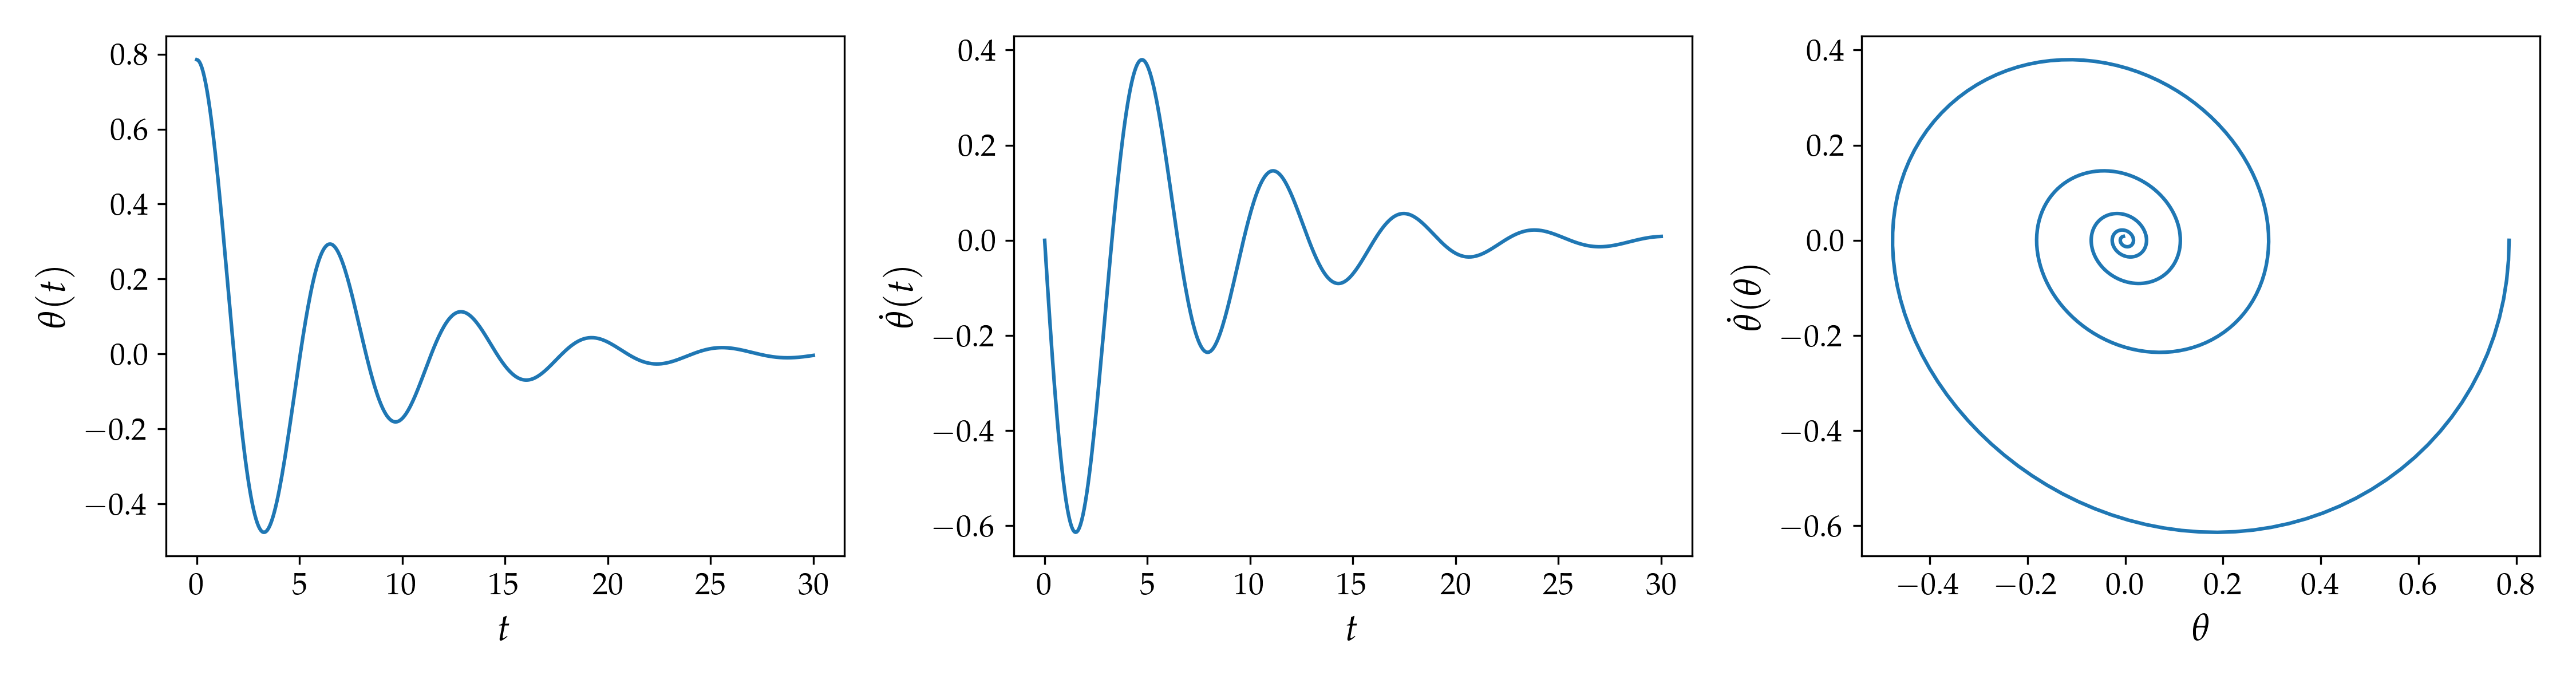
\includegraphics[width=\linewidth]{images/17/17 - 2/A0_g03.png}
    \caption{$A=0, \gamma=0.3$}
    \label{fig: A0_g03}
\end{figure}


\begin{figure}[H]
    \centering
    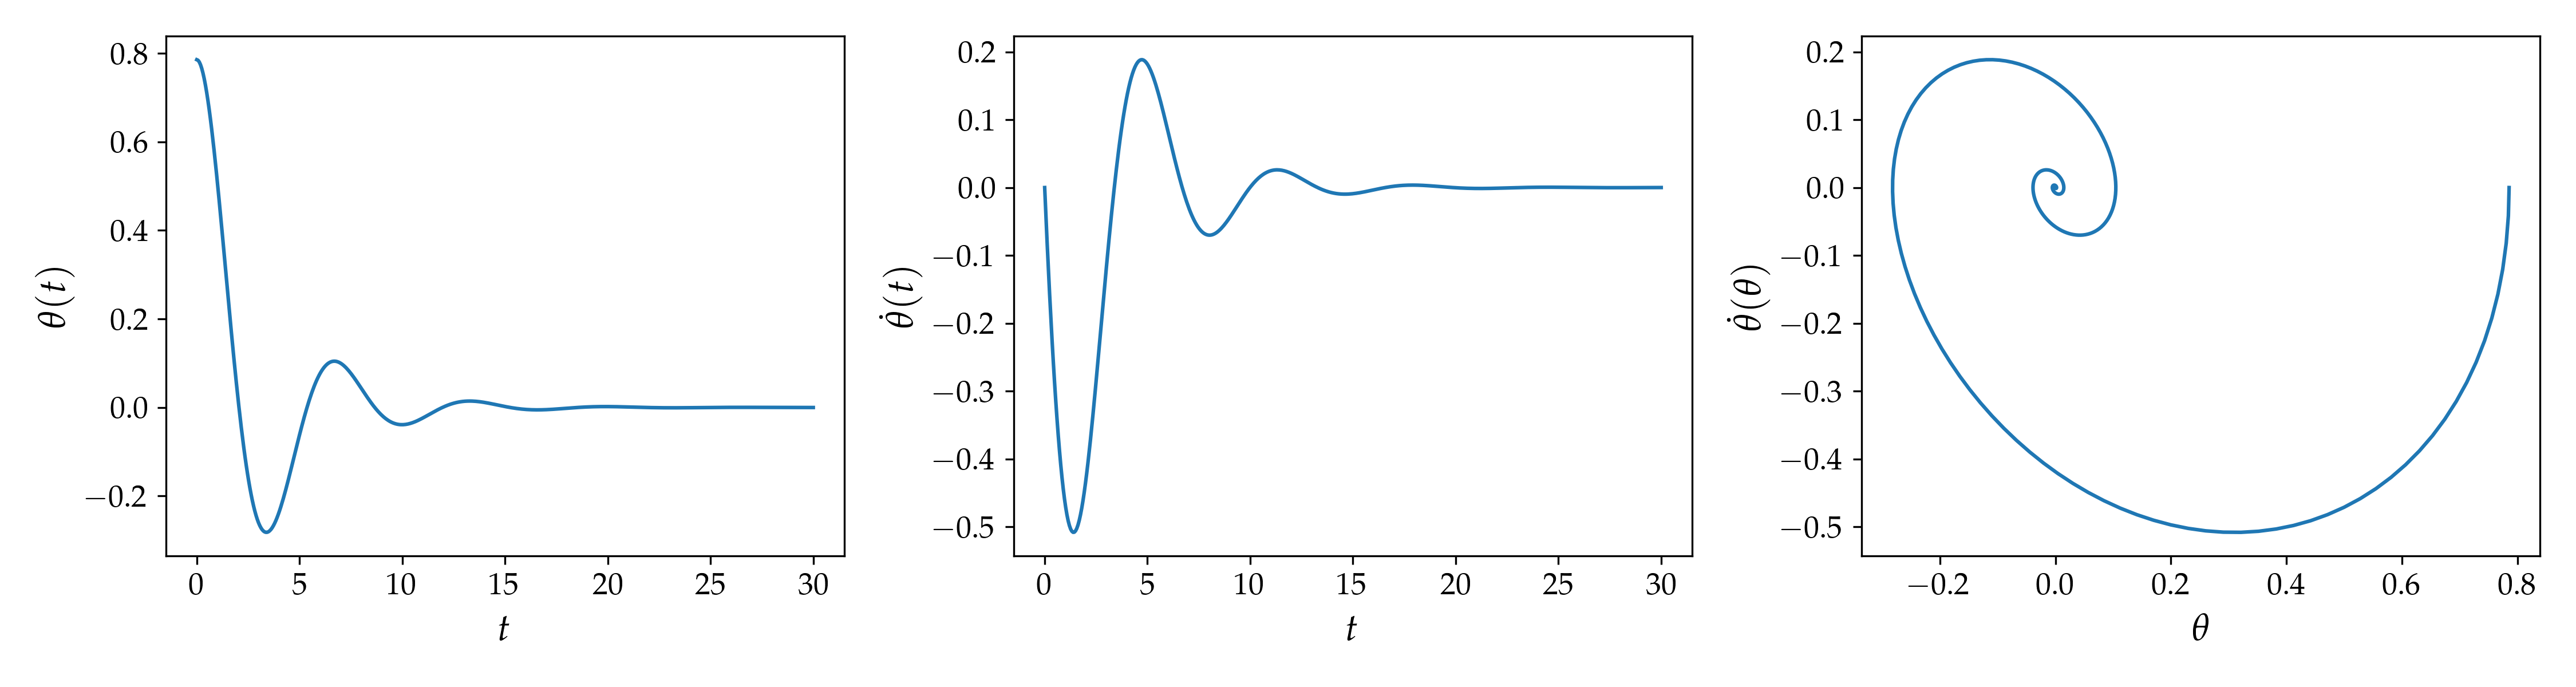
\includegraphics[width=\linewidth]{images/17/17 - 2/A0_g06.png}
    \caption{$A=0, \gamma=0.6$}
    \label{fig: A0_g06}
\end{figure}


\begin{figure}[H]
    \centering
    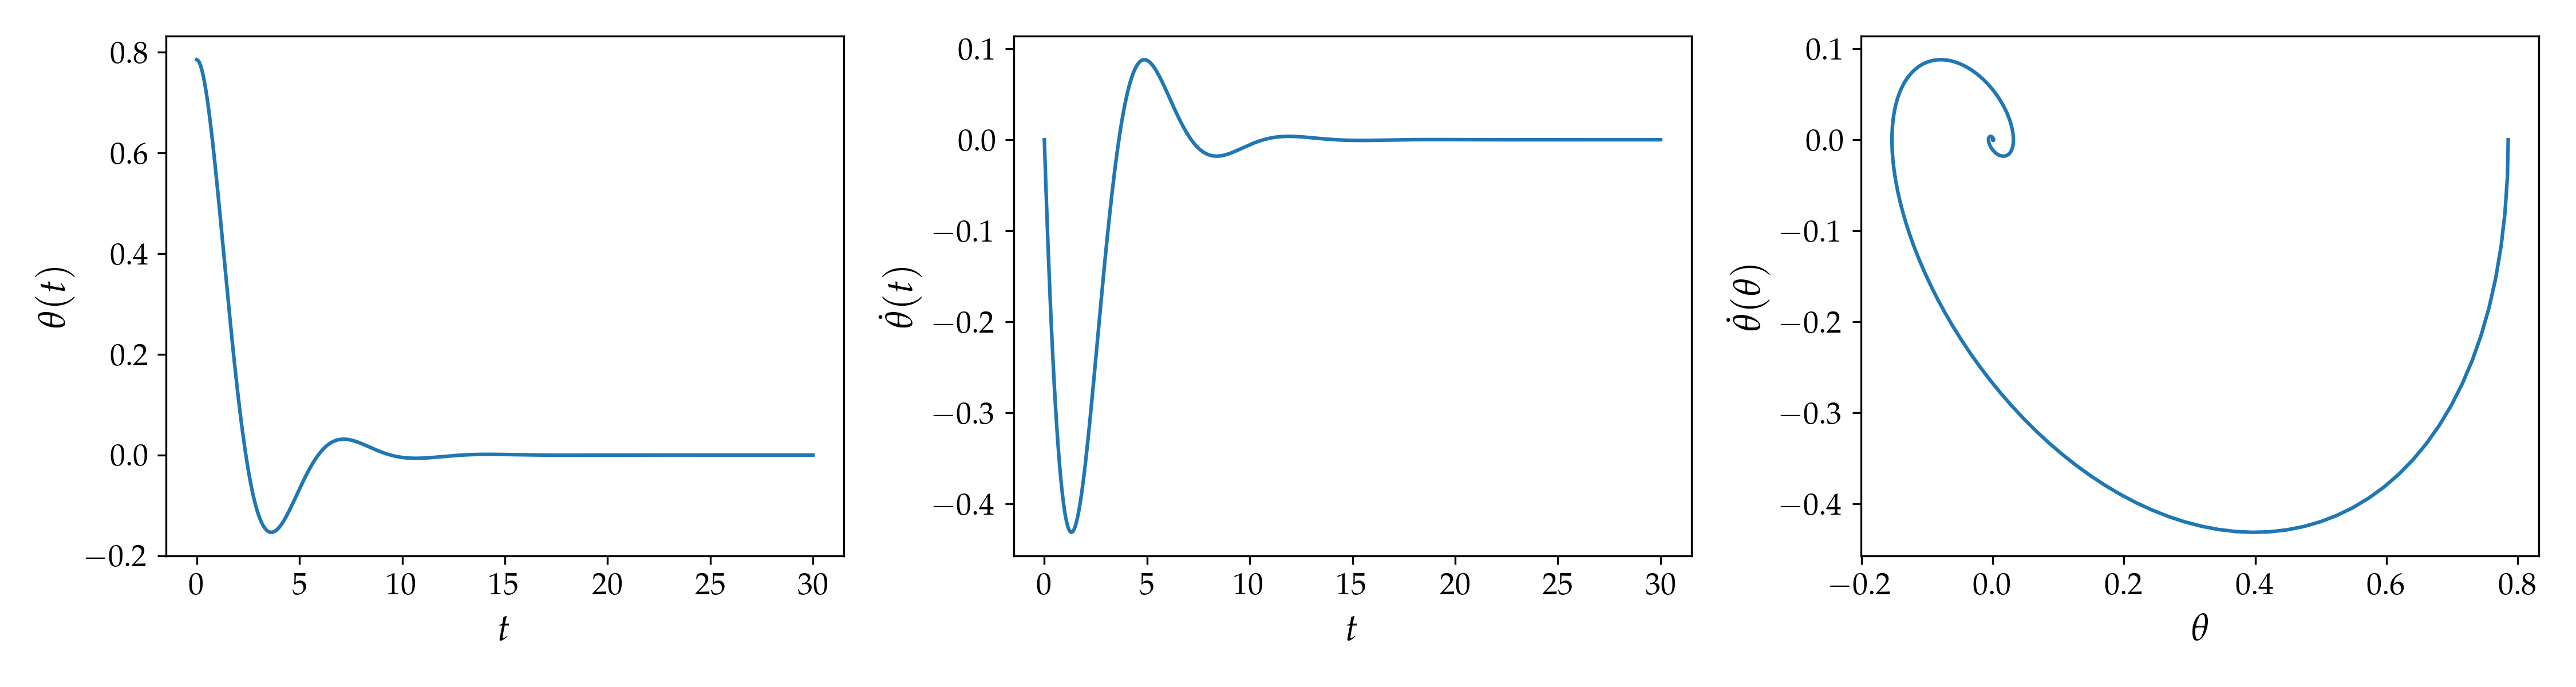
\includegraphics[width=\linewidth]{images/17/17 - 2/A0_g09.png}
    \caption{$A=0, \gamma=0.9$}
    \label{fig: A0_g09}
\end{figure}

\newpage

\begin{figure}[H]
    \centering
    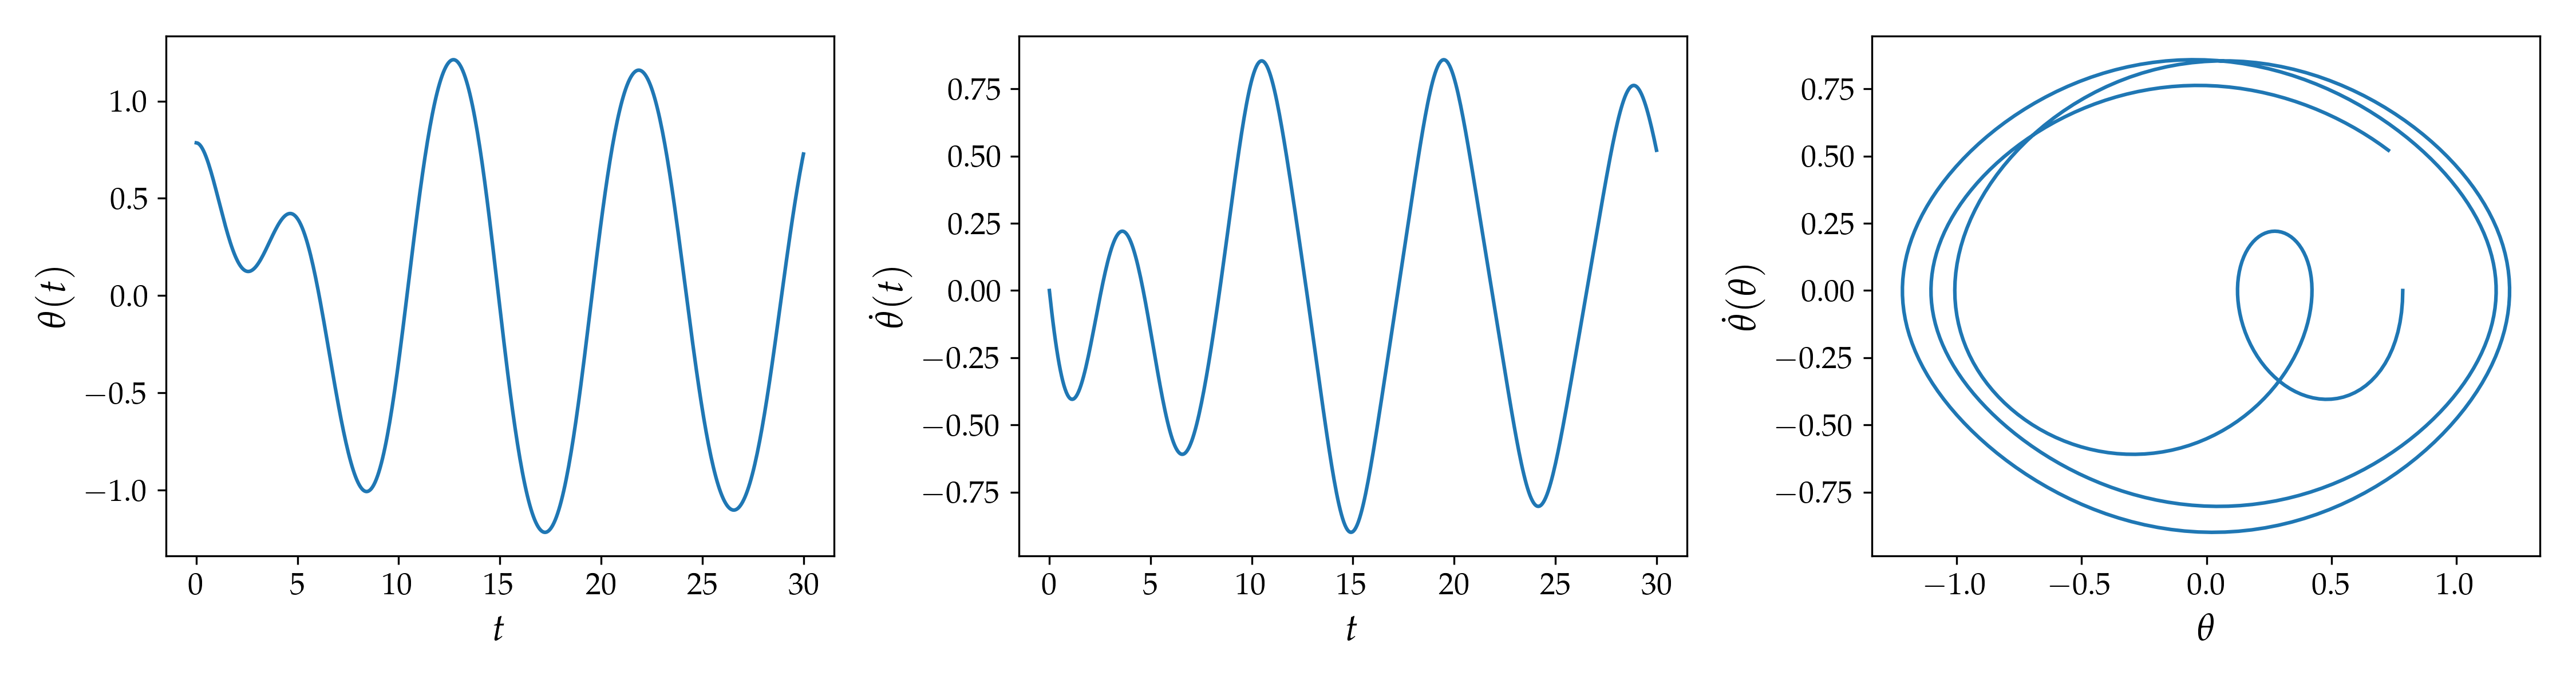
\includegraphics[width=\linewidth]{images/17/17 - 2/A05_g03.png}
    \caption{$A=0.5, \gamma=0.3$}
    \label{fig: A05_g03}
\end{figure}


\begin{figure}[H]
    \centering
    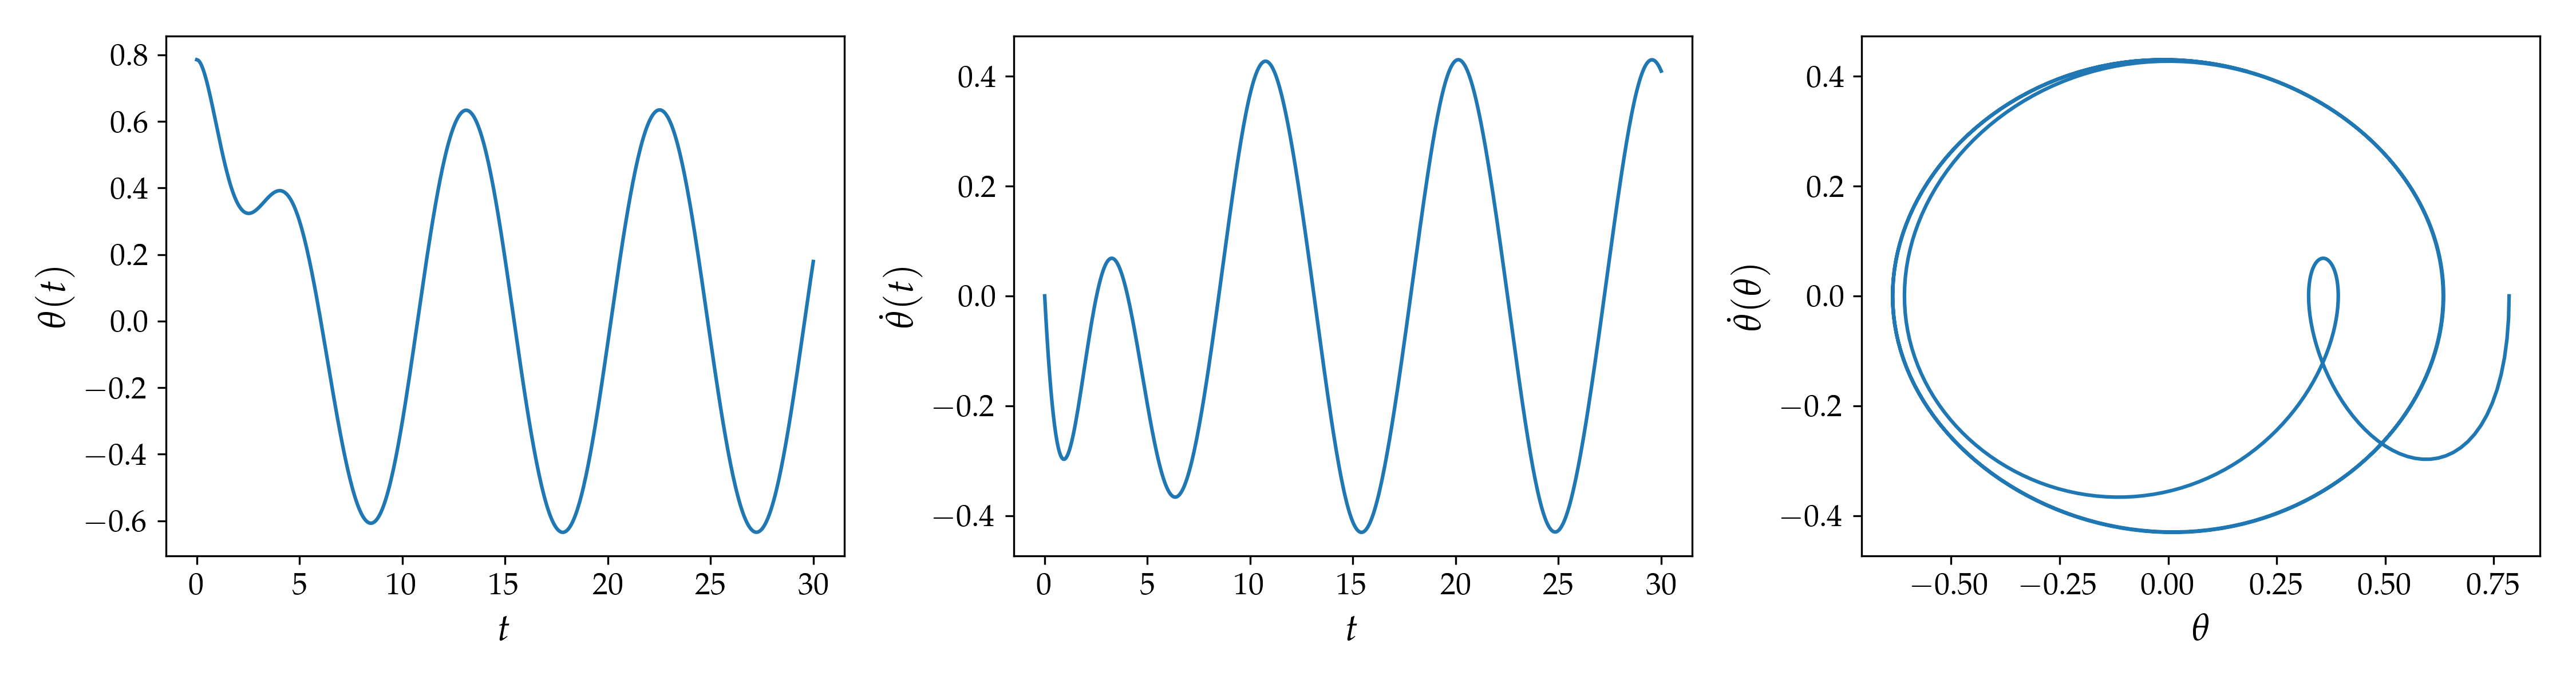
\includegraphics[width=\linewidth]{images/17/17 - 2/A05_g09.png}
    \caption{$A=0.5, \gamma=0.9$}
    \label{fig: A05_g09}
\end{figure}



\begin{figure}[H]
    \centering
    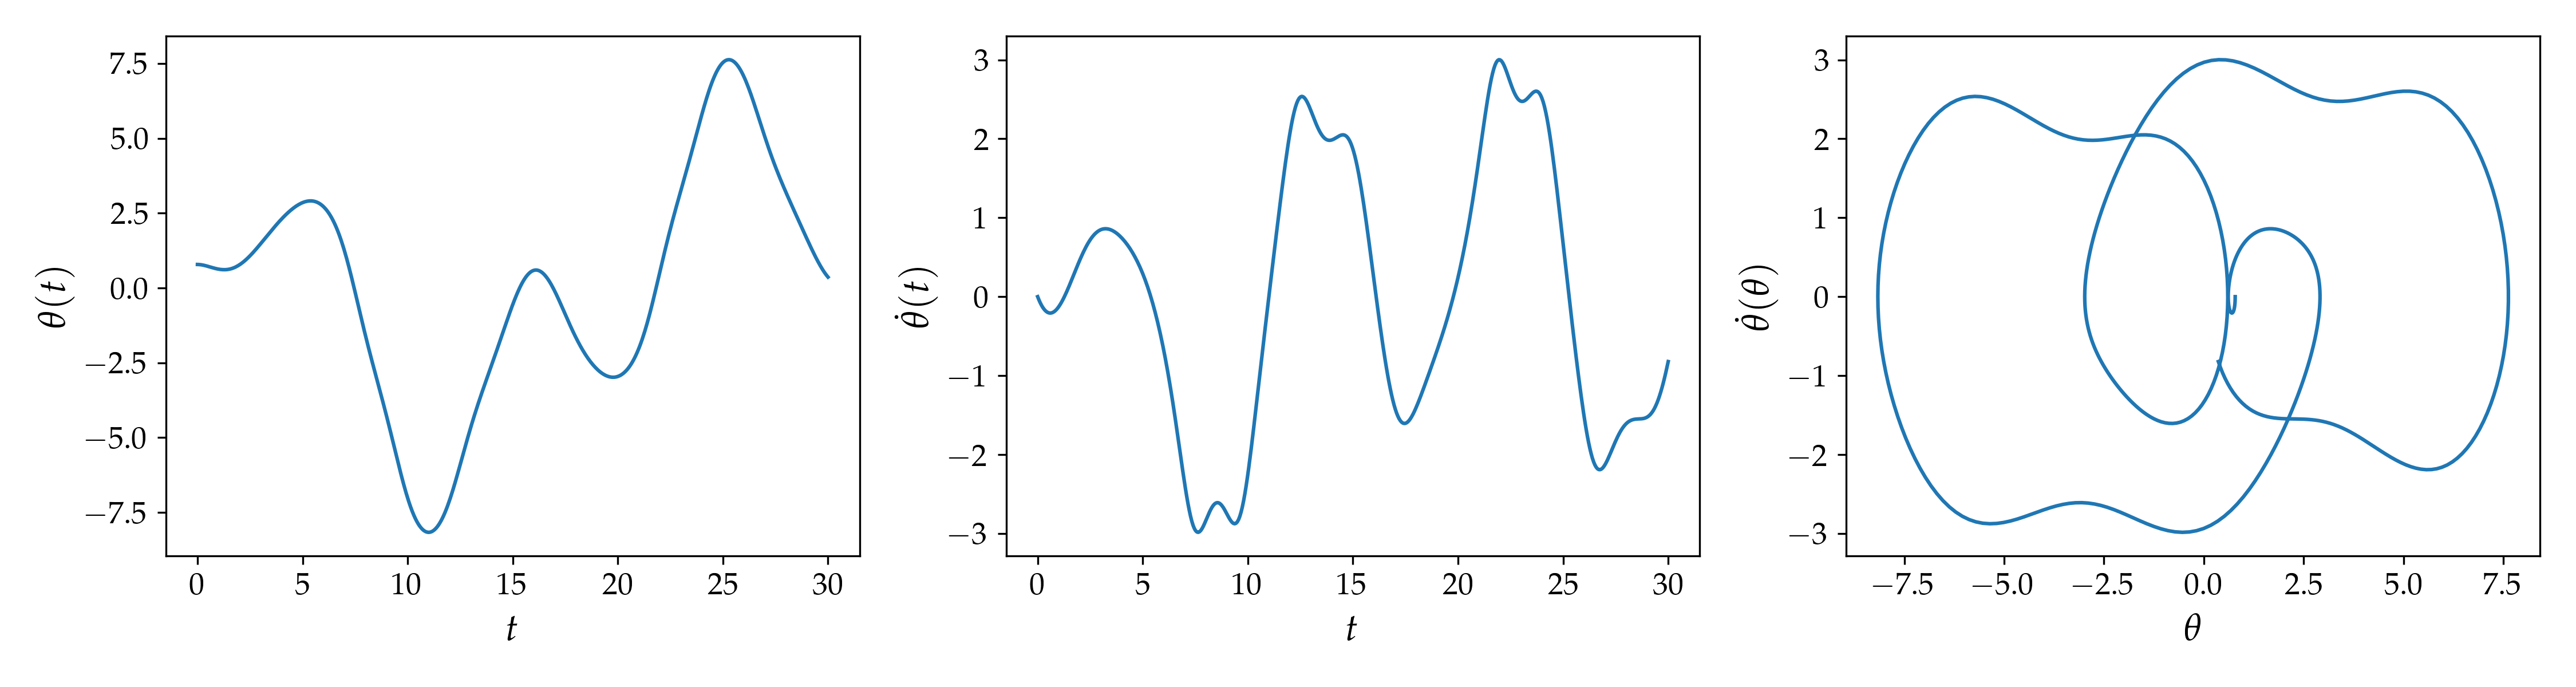
\includegraphics[width=\linewidth]{images/17/17 - 2/A15_g03.png}
    \caption{$A=1.5, \gamma=0.3$}
    \label{fig: A15_g03}
\end{figure}


\begin{figure}[H]
    \centering
    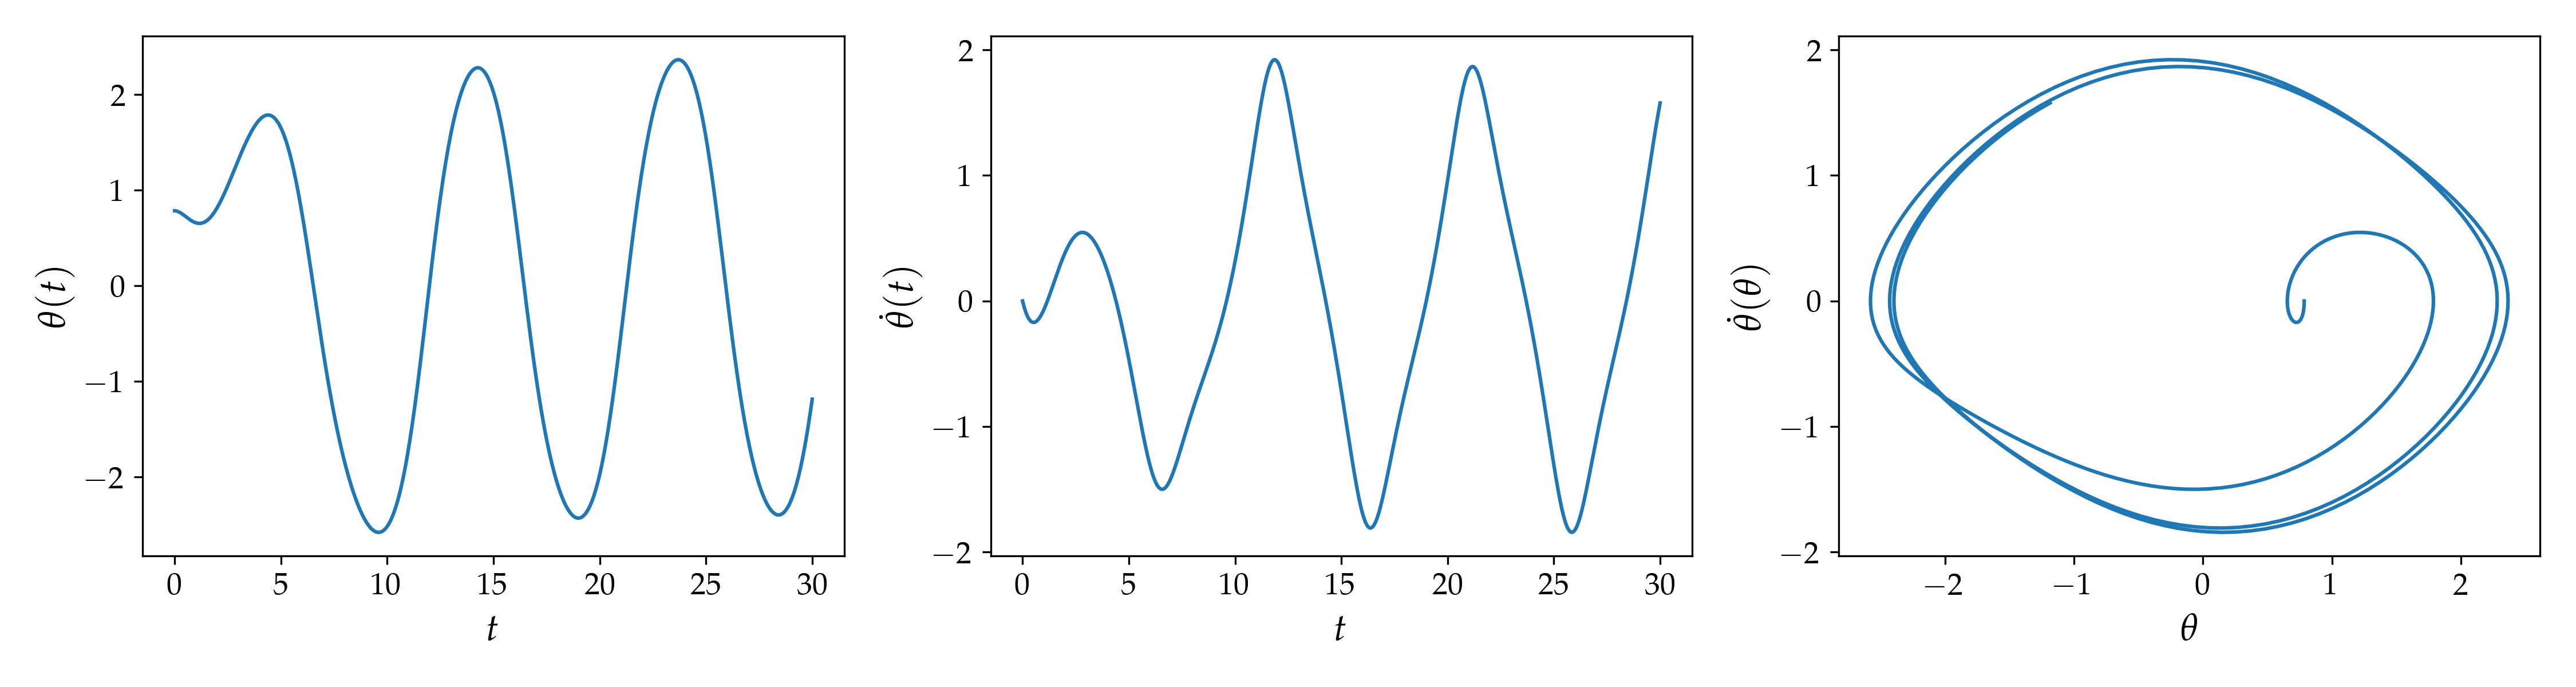
\includegraphics[width=\linewidth]{images/17/17 - 2/A15_g09.png}
    \caption{$A=1.5, \gamma=0.9$}
    \label{fig: A15_g09}
\end{figure}

\noindent Infine procediamo con la valutazione dell'ordine di convergenza del metodo; in particolare con un fit lineare dimostriamo che questo ha scaling di ordine 4.\\
Fissando uno dei diversi casi di indagine come test, si sceglie $A=0, \gamma=0.3$, e un tempo per confrontare le soluzioni al variare solo del passo $h$, scegliamo $t=1$:\\
di seguito la Fig. \ref{fig: fit_rk4} in cui risulta che 
\begin{align*}
    \log_{10}(\mathcal{E(h)}) &\approx a\cdot \log_{10}(h)\\
    \mathcal{E(h)} &\approx h^a, \quad a=4.30
\end{align*}


\begin{figure}[H]
    \centering
    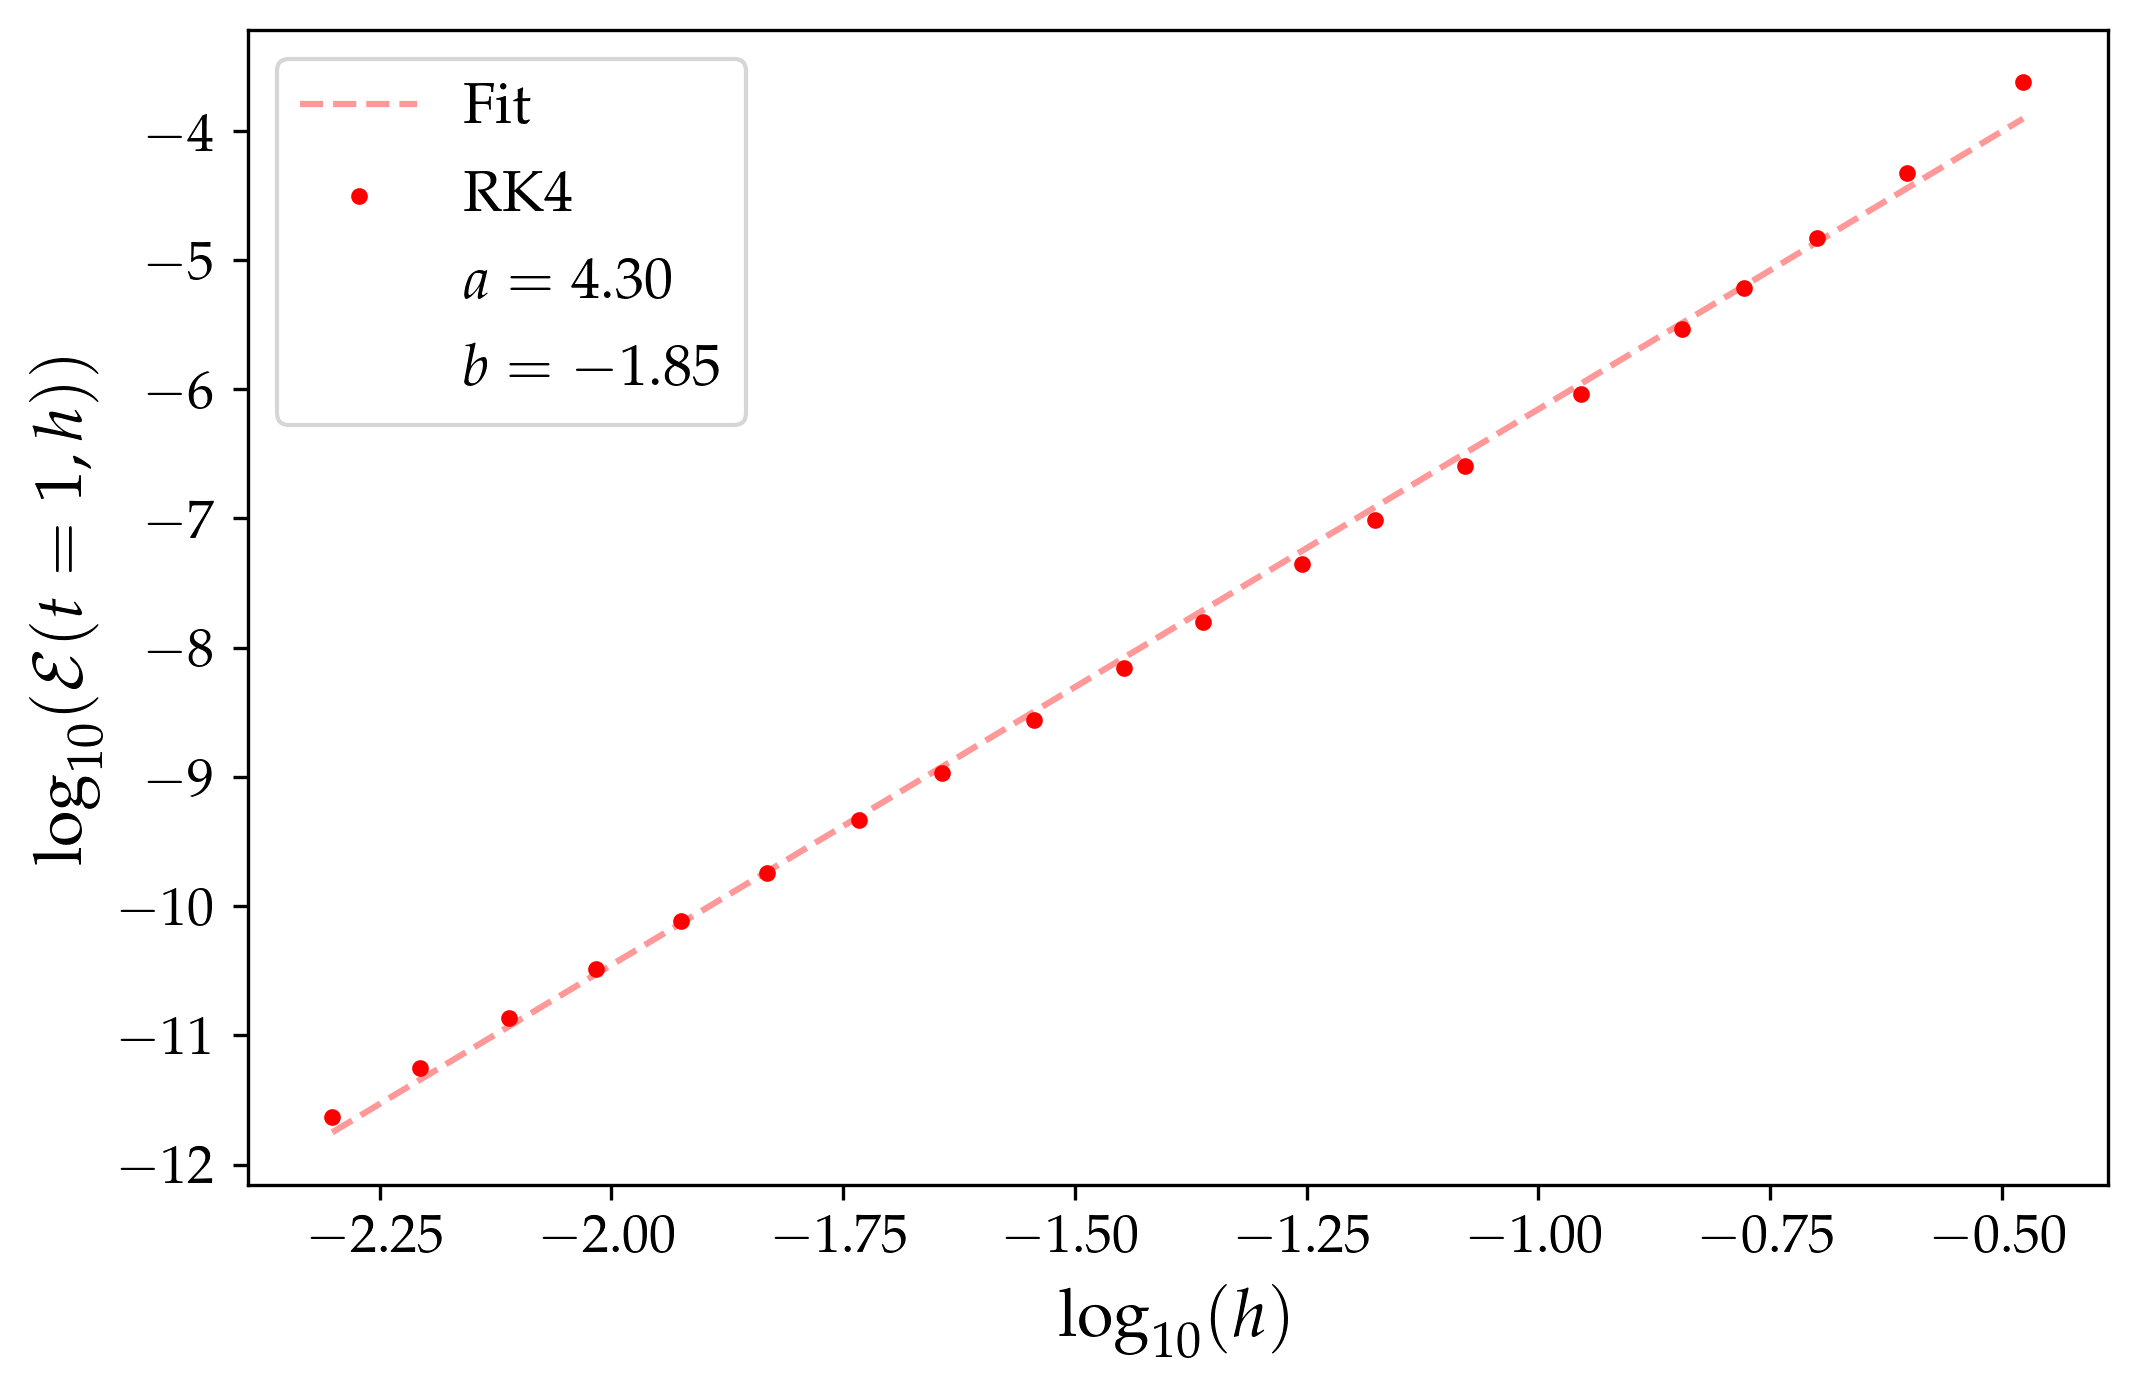
\includegraphics[width=0.8\linewidth]{images/17/17 - 2/fit_rk4.png}
    \caption{Fit del metodo RK4: si verifica la convergenza quartica.}
    \label{fig: fit_rk4}
\end{figure}

\newpage









% \section{Esercizio XXX}
% \subsection{Problem Statement}
% \subsection{Premessa Teorica}
% \subsection{Metodi Numerici e Algoritmi}
% \subsection{Risultati e Discussione}
% \newpage


	

\newpage
% \thispagestyle{empty} 
\null 
\clearpage

% --- PARTE 7: Eq.ne di Schroedinger ---
\cleardoublepage 
\addtocontents{toc}{\bigskip\noindent\protect\textbf{\Large Equazione di Schröedinger}\par\smallskip}
\addtocontents{toc}{\protect\setcounter{tocdepth}{-2}} 
\part{\Huge Equazione di Schröedinger}
\addtocontents{toc}{\protect\setcounter{tocdepth}{2}} 



\section{Esercizio 7.1.1}   \label{Cap. Schr t-indep}
\subsection{Problem Statement}
Per questo esercizio imposta i parametri del sistema fisico a

\begin{itemize}
    \item $mL = 8$
    \item condizioni al contorno aperte $A = B = 0$
    \item $V(x) = \begin{cases} 0 & x < L/4, x \geq 3L/4 \\ -V_0 & L/4 \leq x < 3L/4 \end{cases}$
\end{itemize}

\noindent Scrivi un codice che legga in input il numero di siti del reticolo $N$, $mL$, le condizioni al contorno e $V_0/m$ e restituisca l'operatore Hamiltoniano, che viene poi passato al tuo eigensolver per il calcolo degli autovalori e autovettori.

\noindent Esegui i seguenti compiti:

\begin{enumerate}
    \item Scrivi una funzione per creare un grafico con $E_n/m + \psi_n(x)$ sull'asse verticale per $n = 0, 1, 2, 3$, insieme al potenziale. Usa questa funzione per tracciare le prime 4 autofunzioni $\psi_n(x_i)$ per $V_0/m = 1$ e $N = 64$, e discuti i risultati. C'è una simmetria nel sistema? La osservi? Quali sono le conseguenze?
    \item Ripeti il punto 2 con $V_0/m = -1$ e $N = 64$. Come cambiano le funzioni d'onda e le energie? Spiega il risultato fisico. Sembra esserci una degenerazione approssimata, la comprendi? Nota che non possono esserci stati degeneri in un sistema quantomeccanico 1D.
    \item Traccia l'autofunzione dello stato fondamentale in funzione di $V_0/m = 1, 4, 8$. Spiega il comportamento fisico. Puoi scegliere tra $N = 32$ e $64$.
    \item Imposta $V_0/m = 1$ e calcola il 1°, 4° e 8° autovalore in funzione di $N \in [16, 64]$. Traccia l'autovalore calcolato a un dato $N$ normalizzato per il valore a $N = 64$ in funzione di $N$. Cosa osservi? Perché esibiscono un comportamento/scaling diverso?
    
\end{enumerate}


\subsection{Premessa Teorica}
Vogliamo studiare le soluzioni dell'equazione di Schröedinger indipendente dal tempo (TISE): il potenziale $V$ sarà quindi statico $V = V(x)$.\\
Cercare gli autostati e gli autovalori associati (le energie) equivale a risolvere l'equazione agli autovalori:
$$\left( -\frac{\hbar^2}{2m}\frac{\partial^2}{\partial x^2} + V(x) \right) \phi(x) = E\phi(x)$$
\[
    \hat H \phi(x) = E \phi(x)
\]
La possibilità che abbiamo è quella di attingere ai metodi già implementati per la ricerca di autovalori/vettori (\textit{eigensolver methods}, vedi Parte \ref{cap: Autovalori}).


\subsection{Metodi Numerici e Algoritmi} 
In primis ci occupiamo della discretizzazione delle coordinate, necessaria per la valutazione numerica. Nell'intervallo $[0,L]$ discretizziamo su $N$ intervalli regolari.

\begin{equation*}
    \phi_i = \phi(i \Delta x) \quad \Delta x = L/N
\end{equation*}

\medskip\noindent
Nella definizione dell'hamiltoniana

\begin{align*}
\hat H &= -\frac{\hbar^2}{2m}\frac{\partial^2}{\partial x^2} + V(x)  \\
 &= K+V
\end{align*}

è possibile ridefinire la derivata seconda usando le differenze finite, quindi come:
\[
    \frac{\partial^2}{\partial x^2} \phi(x) \approx \frac{\phi_{i-1} - 2\phi_i + \phi_{i+1} }{\Delta x^2}
\]

\begin{equation*}
    \hat H  \to - \frac{\hbar^2}{2m \Delta x^2} \begin{pmatrix} 
-2 & 1 & 0 & 0 & A \\ 
 1 & -2 & 1 & 0 & 0 \\ 
 0 & 1 & -2 & 1 & 0 \\ 
 0 & 0 & 1 & -2 & 1 \\
 B & 0 & 0 & 1 & -2 \\ 
\end{pmatrix} + \begin{pmatrix} 
V_0 & 0 & 0 & 0 & 0 \\
0 & V_1 & 0 & 0 & 0 \\
0 & 0 & V_2 & 0 & 0 \\
0 & 0 & 0 & V_3 & 0 \\
0 & 0 & 0 & 0 & V_4 \\
\end{pmatrix} = - \frac{\hbar^2}{2m \Delta x^2} K_d + V
\end{equation*}

\noindent dove $K_d$ indica esclusivamente la matrice tridiagonale adimensionale dei coefficienti di accoppiamento. L'operatore differenziale della derivata seconda sullo spazio discreto è quindi recuperato tramite il prodotto $\frac{1}{\Delta x^2}K_d$.

\medskip\noindent
In unità naturali $\hbar = 1$ e riscriviamo tutto in forma adimensionale:
\begin{equation*}
    - \frac{1}{2m \Delta x^2} K_d = - \frac{N^2 }{2 (mL) L} K_d 
\end{equation*}


\begin{equation*}
    \left[ - \frac{N^2}{2 (mL)^2} K_d + \mathcal V \right] \phi = \mathcal E \phi \qquad \mathcal E = E/m \,, \mathcal V = V/m
\end{equation*}

\medskip\noindent
L'utilizzo del \textit{QR eigensolver} è possibile per la risoluzione del problema.


\subsection{Risultati e Discussione}
Vengono fissati $N=64, mL=8$. Si noti che per tutti i plot dell'esercizio $\phi(mx)$, che è una funzione a valori nei complessi, viene rappresentata solo nella sua componente reale.

\subsubsection{Autostati della buca finita}
Dalla teoria ci aspettiamo di trovare due tipologie di autostati:
\begin{itemize}
    \item \textbf{Bound states} o \textbf{stati legati}: corrispondono alle energie minori dell'altezza della buca, quindi dove la particella rimane confinata nella buca. Lo spettro è discreto.
    \item \textbf{Scattering states} o \textbf{stati non legati}: corrispondono a energie maggiori dell'altezza della buca, dove la particella si muove come un'onda piana, con frequenza di oscillazione variabile. Lo spettro è continuo. Lo spettro continuo è possibile nel calcolo numerico solo con una matrice di dimensione infinita (non discretizzata): i risultati numerici sono quindi approssimazioni degli infiniti autostati dello spettro continuo, sotto discretizzazione finita.
\end{itemize}

\noindent Inoltre sappiamo che per un potenziale simmetrico gli autostati hanno parità definita; si alterneranno quindi autofunzioni pari e dispari. Tutto ciò è visibile in Fig. \ref{fig: fin_well}: si osservano le $\phi$ che decadono sotto la buca e quelle che invece rimangono oscillanti, si può osservare che se disegniamo $\phi(-x)$ e la sovrapponiamo al grafico, possiamo distinguere gli stati pari (le due autofunzioni sono sovrapposte) da quelli dispari (una è la speculare dell'altra).\\
Inoltre in Fig. \ref{fig: fin_well_mod2} osserviamo il modulo quadro delle funzioni d'onda che rappresenta la probabilità relativa all'esito di una misura.

\begin{figure}[H]
    \centering
    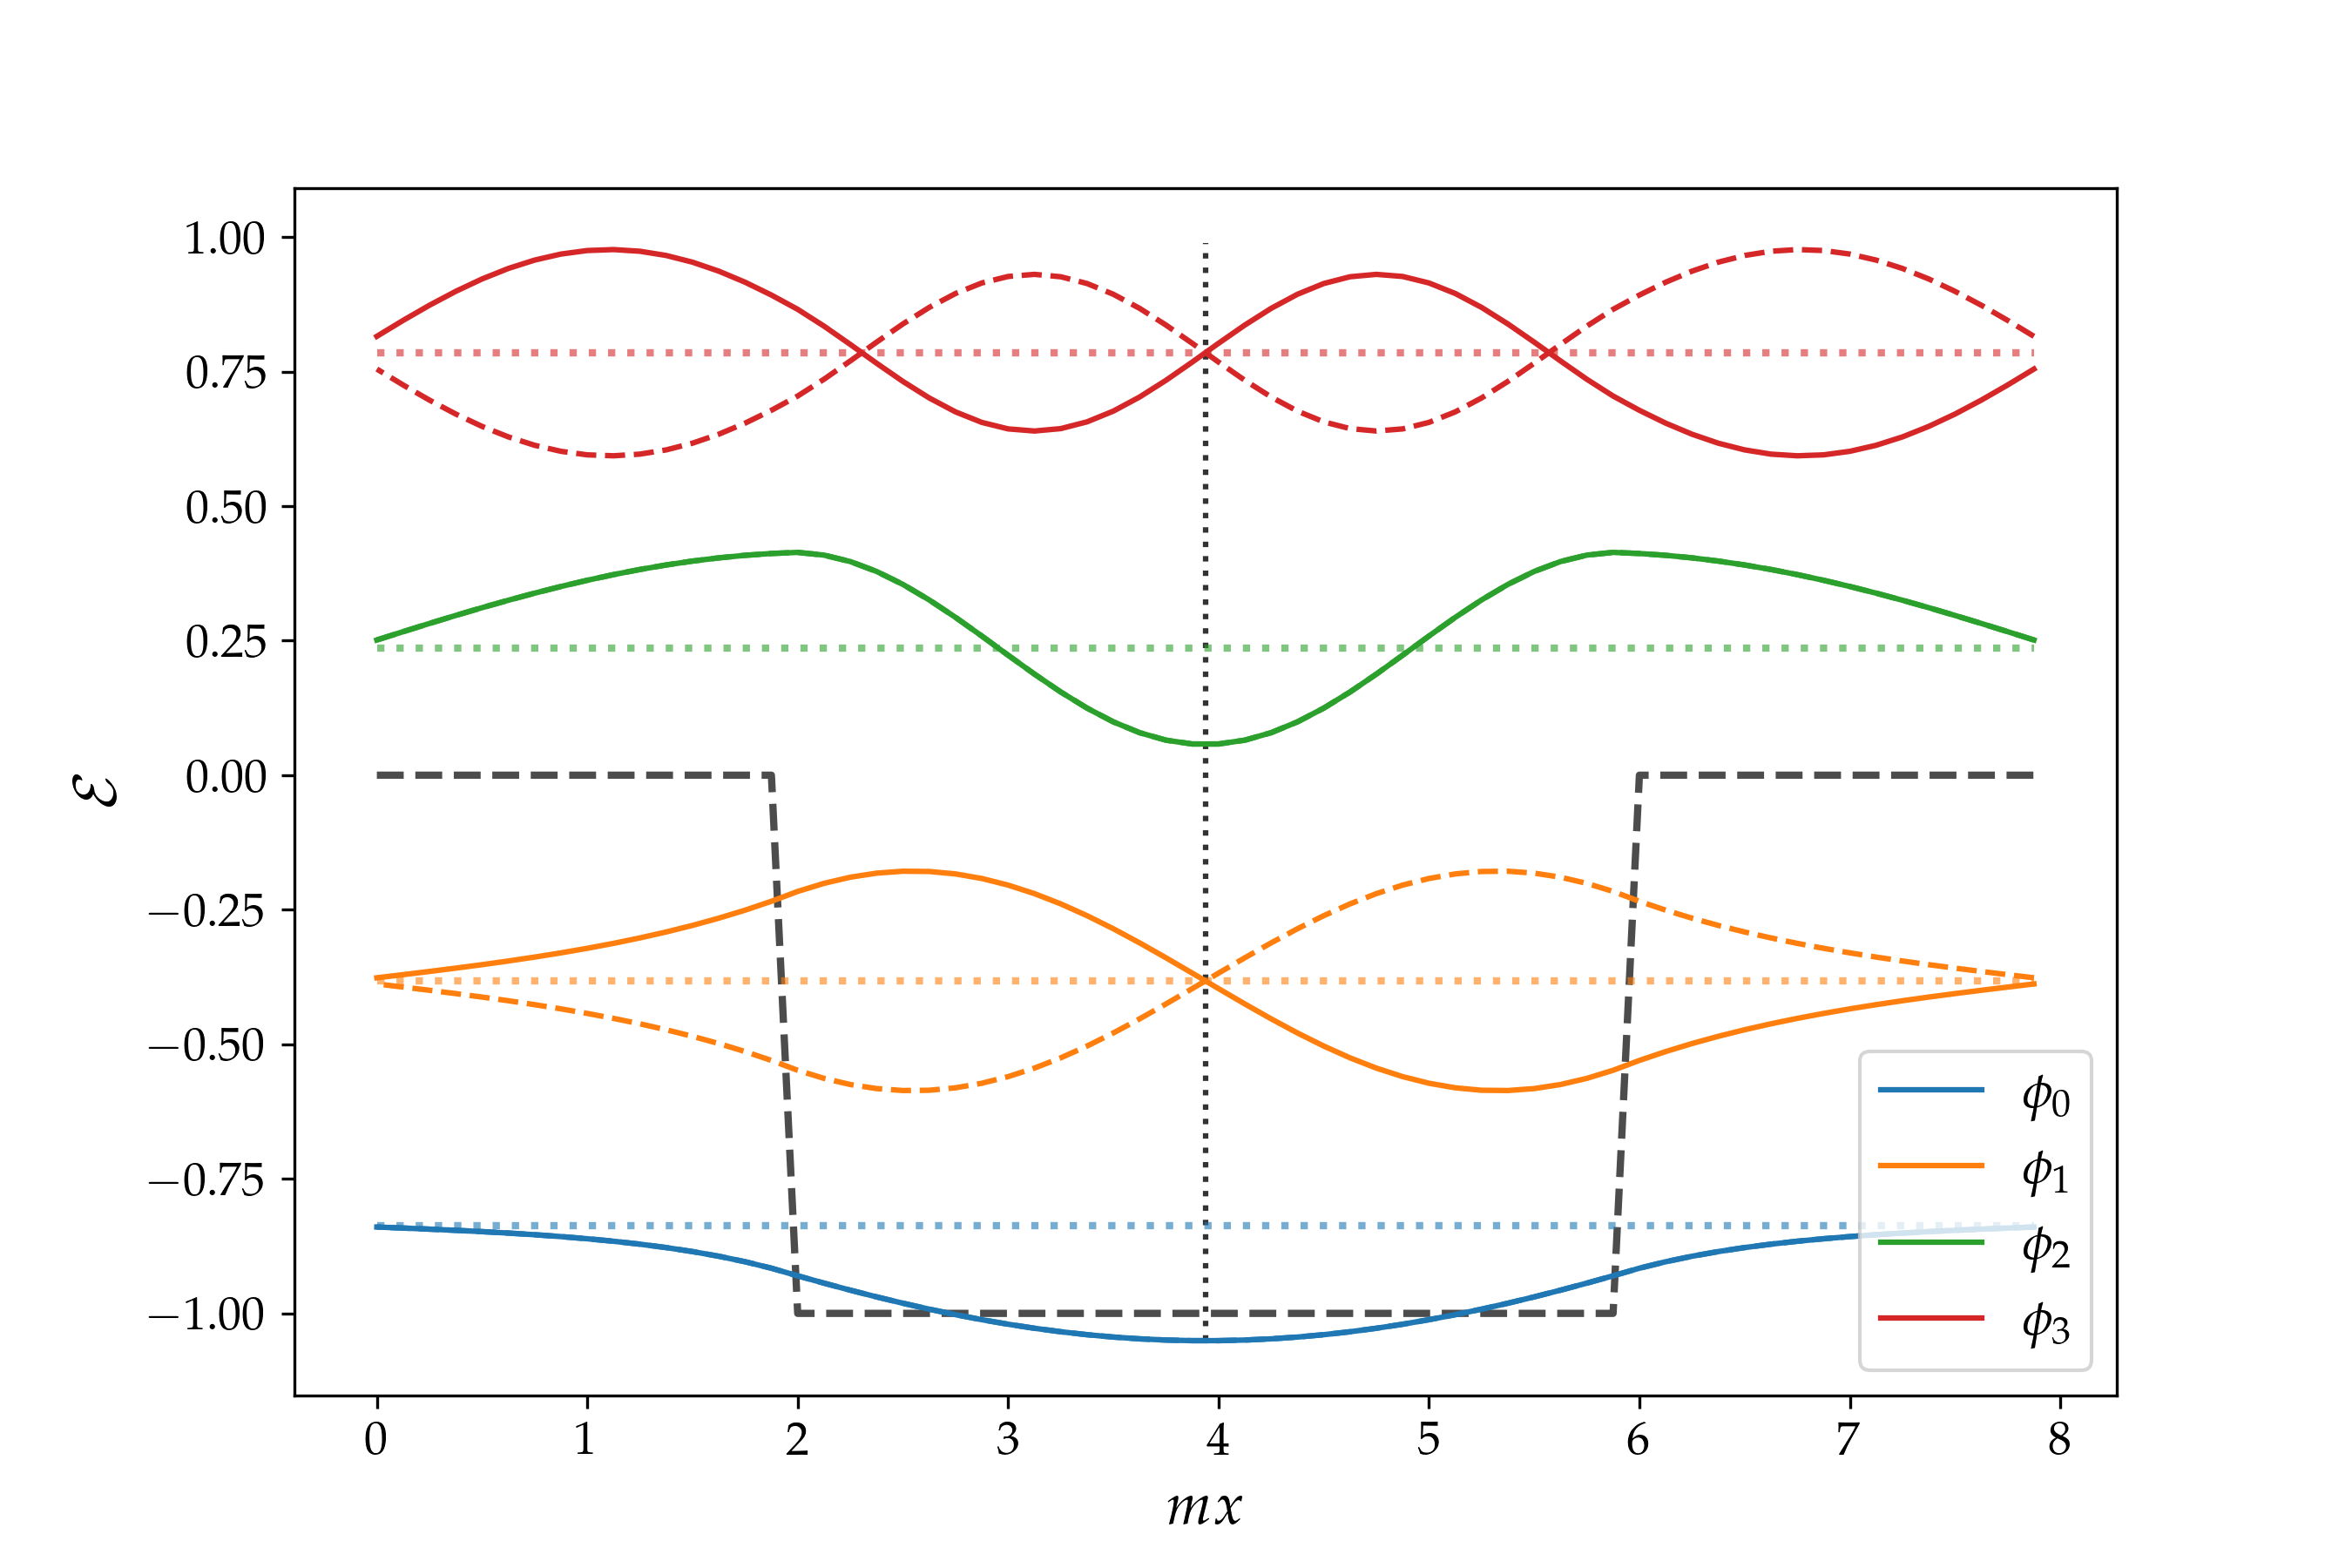
\includegraphics[width=0.7\linewidth]{images/18/finite_well.png}z
    \caption{I primi quattro autostati della buca finita e i relativi autovalori. In linea continua le autofunzioni $\phi_i$, in linea tratteggiata colorata le autofunzioni con parità invertita: $\phi(mx) \to \phi(-mx)$. $\phi_0$ rappresenta il \textit{ground state}. In linea tratteggiata nera il potenziale della buca.}
    \label{fig: fin_well}
\end{figure}

\begin{figure}[H]
    \centering
    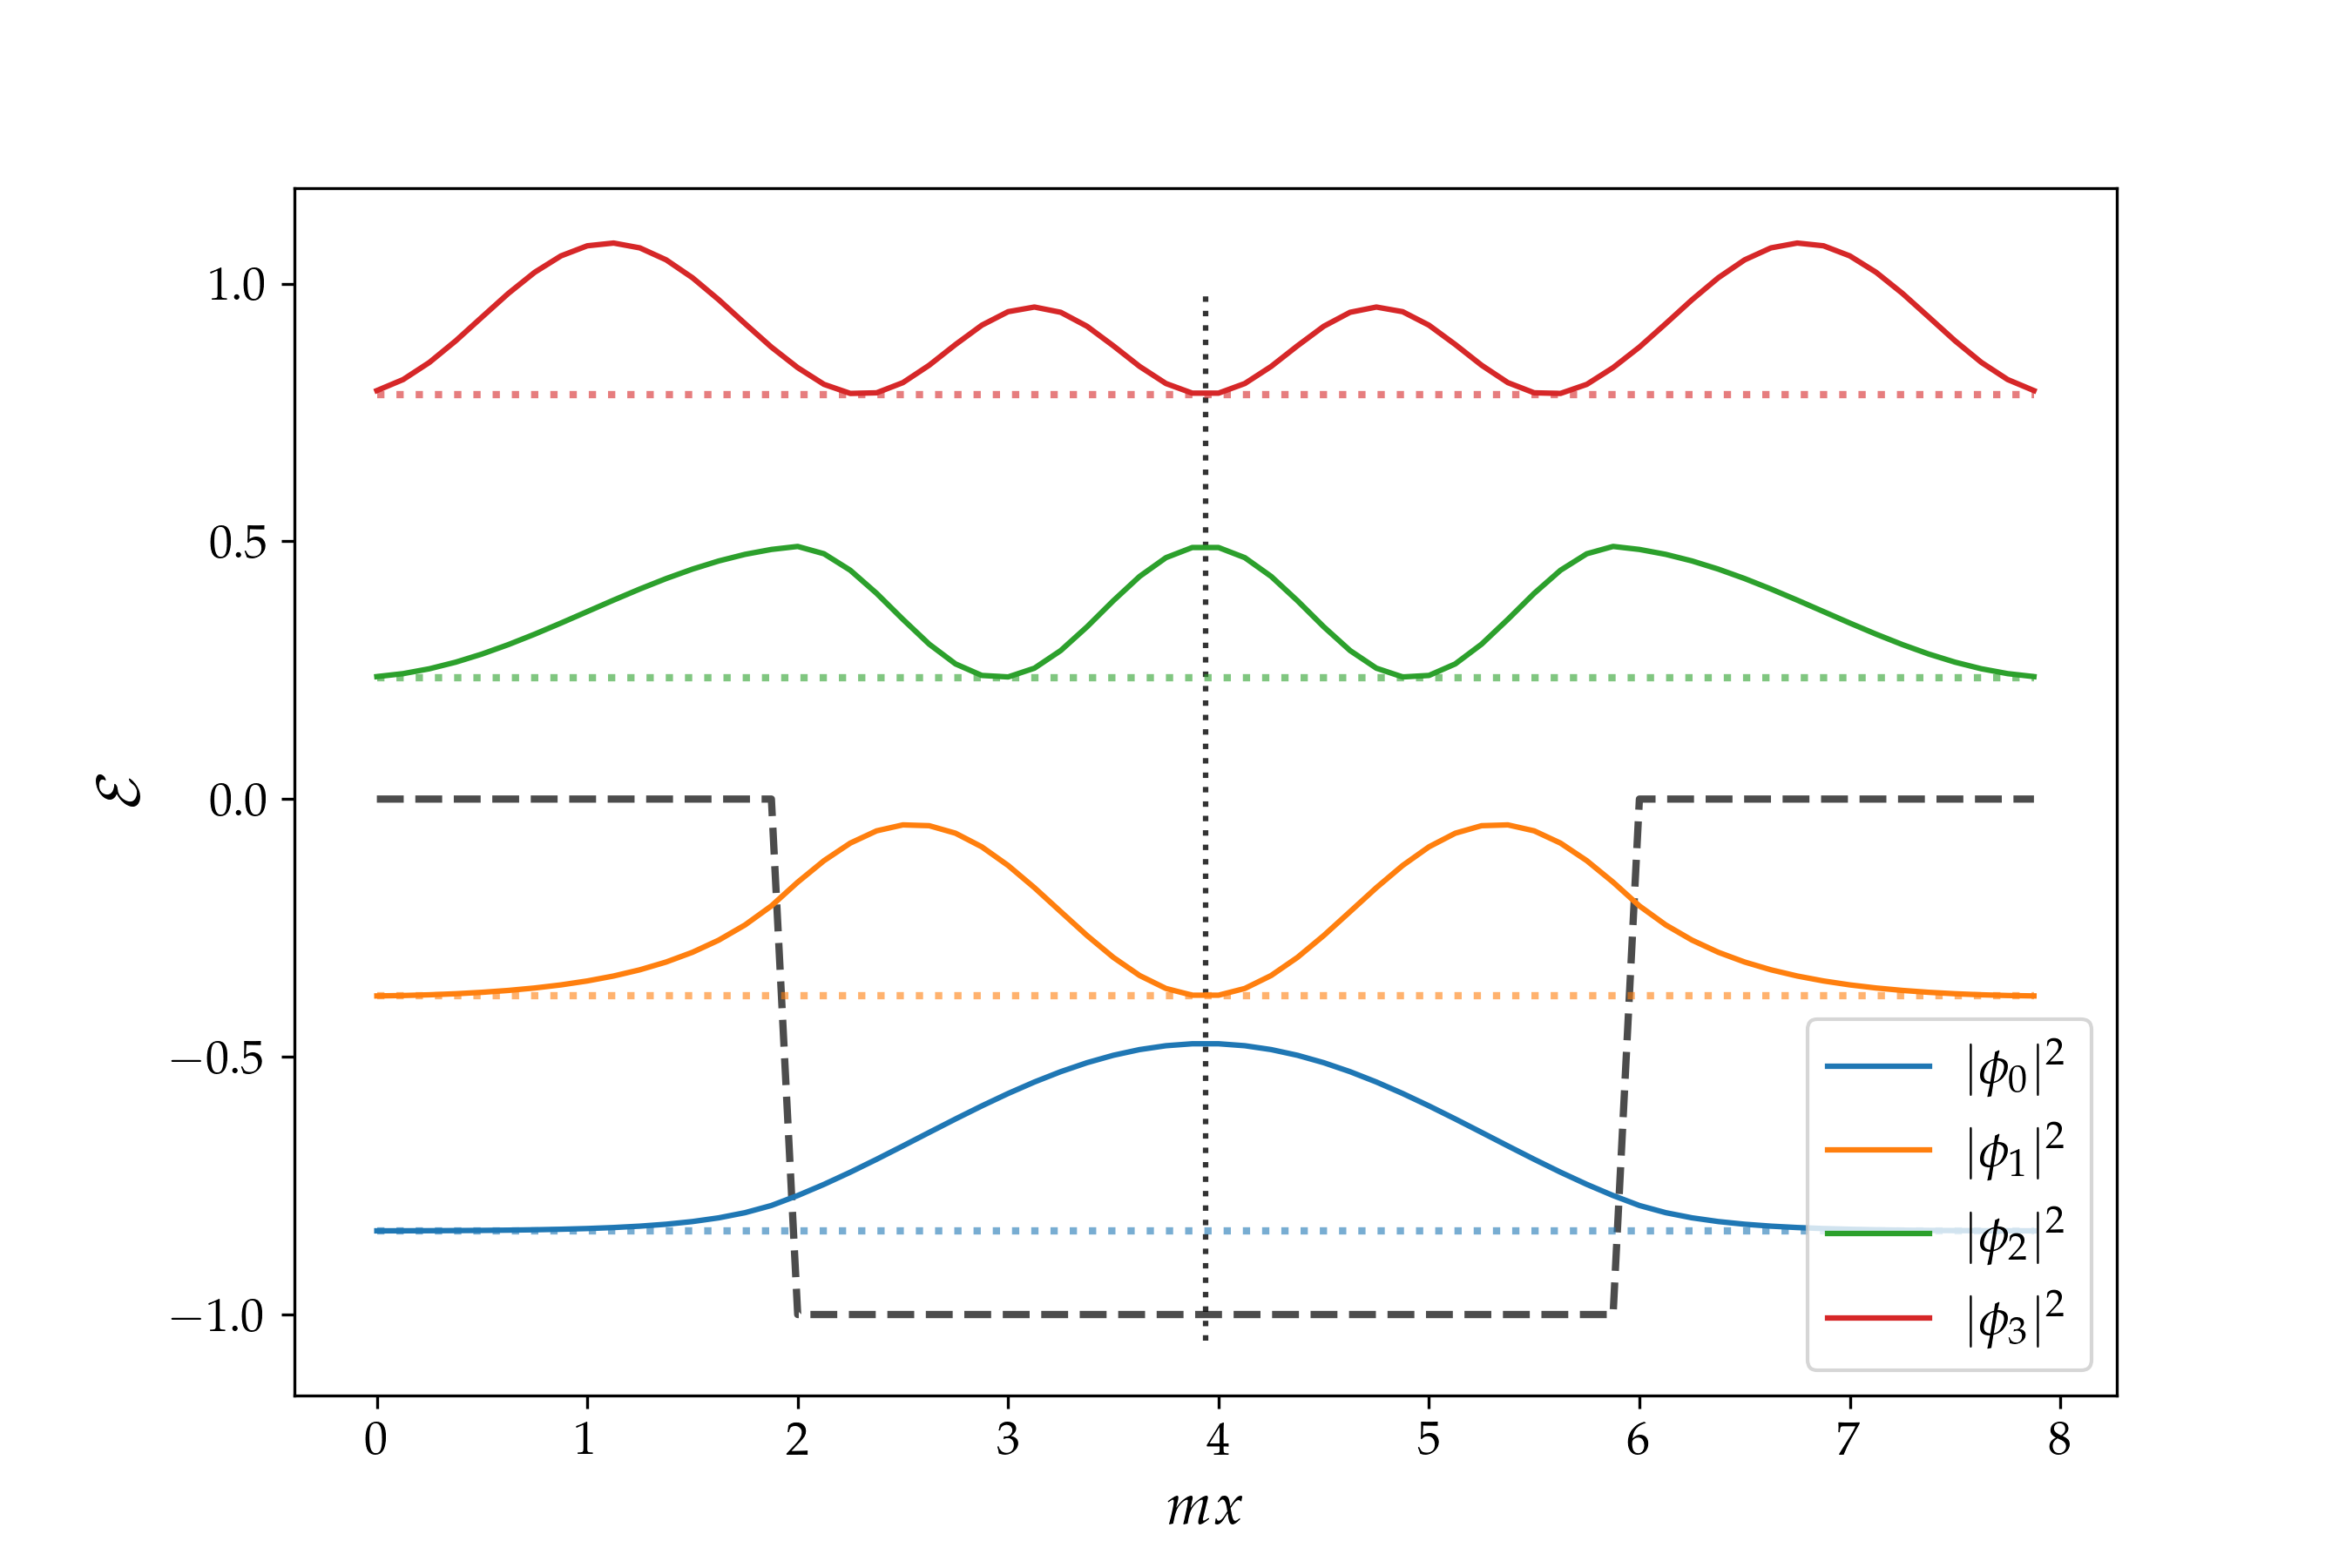
\includegraphics[width=0.7\linewidth]{images/18/finite_well_mod2.png}
    \caption{Modulo quadro dei primi quattro autostati della buca finita.}
    \label{fig: fin_well_mod2}
\end{figure}



\subsubsection{Autostati della barriera finita}
Con $V_0/m = -1$ abbiamo il potenziale di una barriera rettangolare finita. Si osservano due effetti particolari:
\begin{itemize}
    \item Agli autovalori inferiori all'altezza della barriera sono associate autofunzioni che decadono esponenzialmente sotto il potenziale: quello che si osserva è il fenomeno di tunneling quantistico, cioè la probabilità che la particella superi la barriera è non nulla.
    \item Questo sistema evidenzia una simil degenerazione: due livelli energetici sono molto simili\\($\mathcal{E}_1 \approx 0.58, \mathcal{E}_2 \approx 0.59$): in un sistema 1D non è possibile ottenere delle degenerazioni esatte ($\mathcal{E}_i = \mathcal{E}_j$ implicherebbe che le due autofunzioni siano linearmente dipendenti, quindi lo stesso autostato a meno di una fase).
\end{itemize}

\noindent Possiamo immaginare questa configurazione come l'approssimazione di due buche separate da una barriera. Se la barriera è infinita i due sistemi sono isolati e non possono interagire: gli stati fondamentali sono $\psi_L, \psi_R$. Immaginiamo di modificare il sistema e di rendere la barriera finita; le due fdo possono interagire e sovrapporsi. Introducendo l'elemento di matrice $$t=\langle\psi_L|\hat H| \psi_R \rangle = \langle\psi_R|\hat H| \psi_L \rangle$$
che rappresenta il termine di accoppiamento dovuto all'interazione tra $L$ e $R$, possiamo studiare gli autostati/valori di questo nuovo sistema:
\begin{align*}
    H = 
    \begin{pmatrix}
        E_0 & t \\
        t & E_0
    \end{pmatrix}
\end{align*}

dove 
\begin{align*}
    |\psi_L\rangle = \begin{pmatrix}
        1\\
        0
    \end{pmatrix}, \quad    
    |\psi_R\rangle = \begin{pmatrix}
        0\\
        1
    \end{pmatrix}    
\end{align*}

\begin{align*}
    \hat H|\psi_L\rangle &=  E_0 |\psi_L\rangle + t|\psi_R\rangle\\
    \hat H|\psi_R\rangle &=  E_0 |\psi_R\rangle + t|\psi_L\rangle
\end{align*}

diagonalizzando la matrice troviamo gli autovalori, in particolare:
\begin{align*}
    \det(H- EI) & =(E_0- E)^2 - t^2 = 0\\
    \implies \quad & E = E_0 \pm |t|
\end{align*}

\noindent Le autofunzioni associate:
\begin{itemize}

    \item $E = E_0 - |t|$\\
    L'autovettore è 
        \begin{pmatrix}
            1\\
            1
        \end{pmatrix}
    \[
    \boldsymbol v_S = \frac{1}{\sqrt{2}} (|\psi_L\rangle + |\psi_R\rangle)
    \]

    L'autostato sul livello energetico più basso, il \textit{GS}, è quello dato dalla sovrapposizione simmetrica delle due autofunzioni delle buche.

    \item $E = E_0 + |t|$\\
    L'autovettore è 
        \begin{pmatrix}
            1\\
            -1
        \end{pmatrix}
    \[
    \boldsymbol v_A = \frac{1}{\sqrt{2}} (|\psi_L\rangle - |\psi_R\rangle)
    \]
    cioè individuiamo lo stato antisimmetrico come quello più energetico.
\end{itemize}

\noindent Questa separazione sussiste dal momento che abbiamo aggiunto un termine che permette l'interazione tra le due funzioni d'onda, cioè dal momento che abbiamo impostato una barriera finita, cioè che permette tunneling: ci aspettiamo che la separazione dei due stati aumenti all'aumentare dell'interazione tra le due $|\psi_L\rangle, |\psi_R\rangle$, cioè all'abbassarsi della barriera, o al suo assottigliamento. Il caso limite diventa l'eliminazione della stessa, che ci riporta in una configurazione con due stati nettamente separati, cioè quella della buca infinita.\\
D'altra parte vi è il caso della barriera sempre più alta, che fa diminuire l'accoppiamento tra gli stati, avvicinando i livelli energetici. Il caso limite diventa chiaramente quello con cui eravamo partiti; due buche infinite separate. Le due funzioni sono relative ad un potenziale simmetrico, indi per cui le soluzioni sono necessariamente simmetriche (e in questo caso identiche).
\begin{figure}[H]
    \centering
    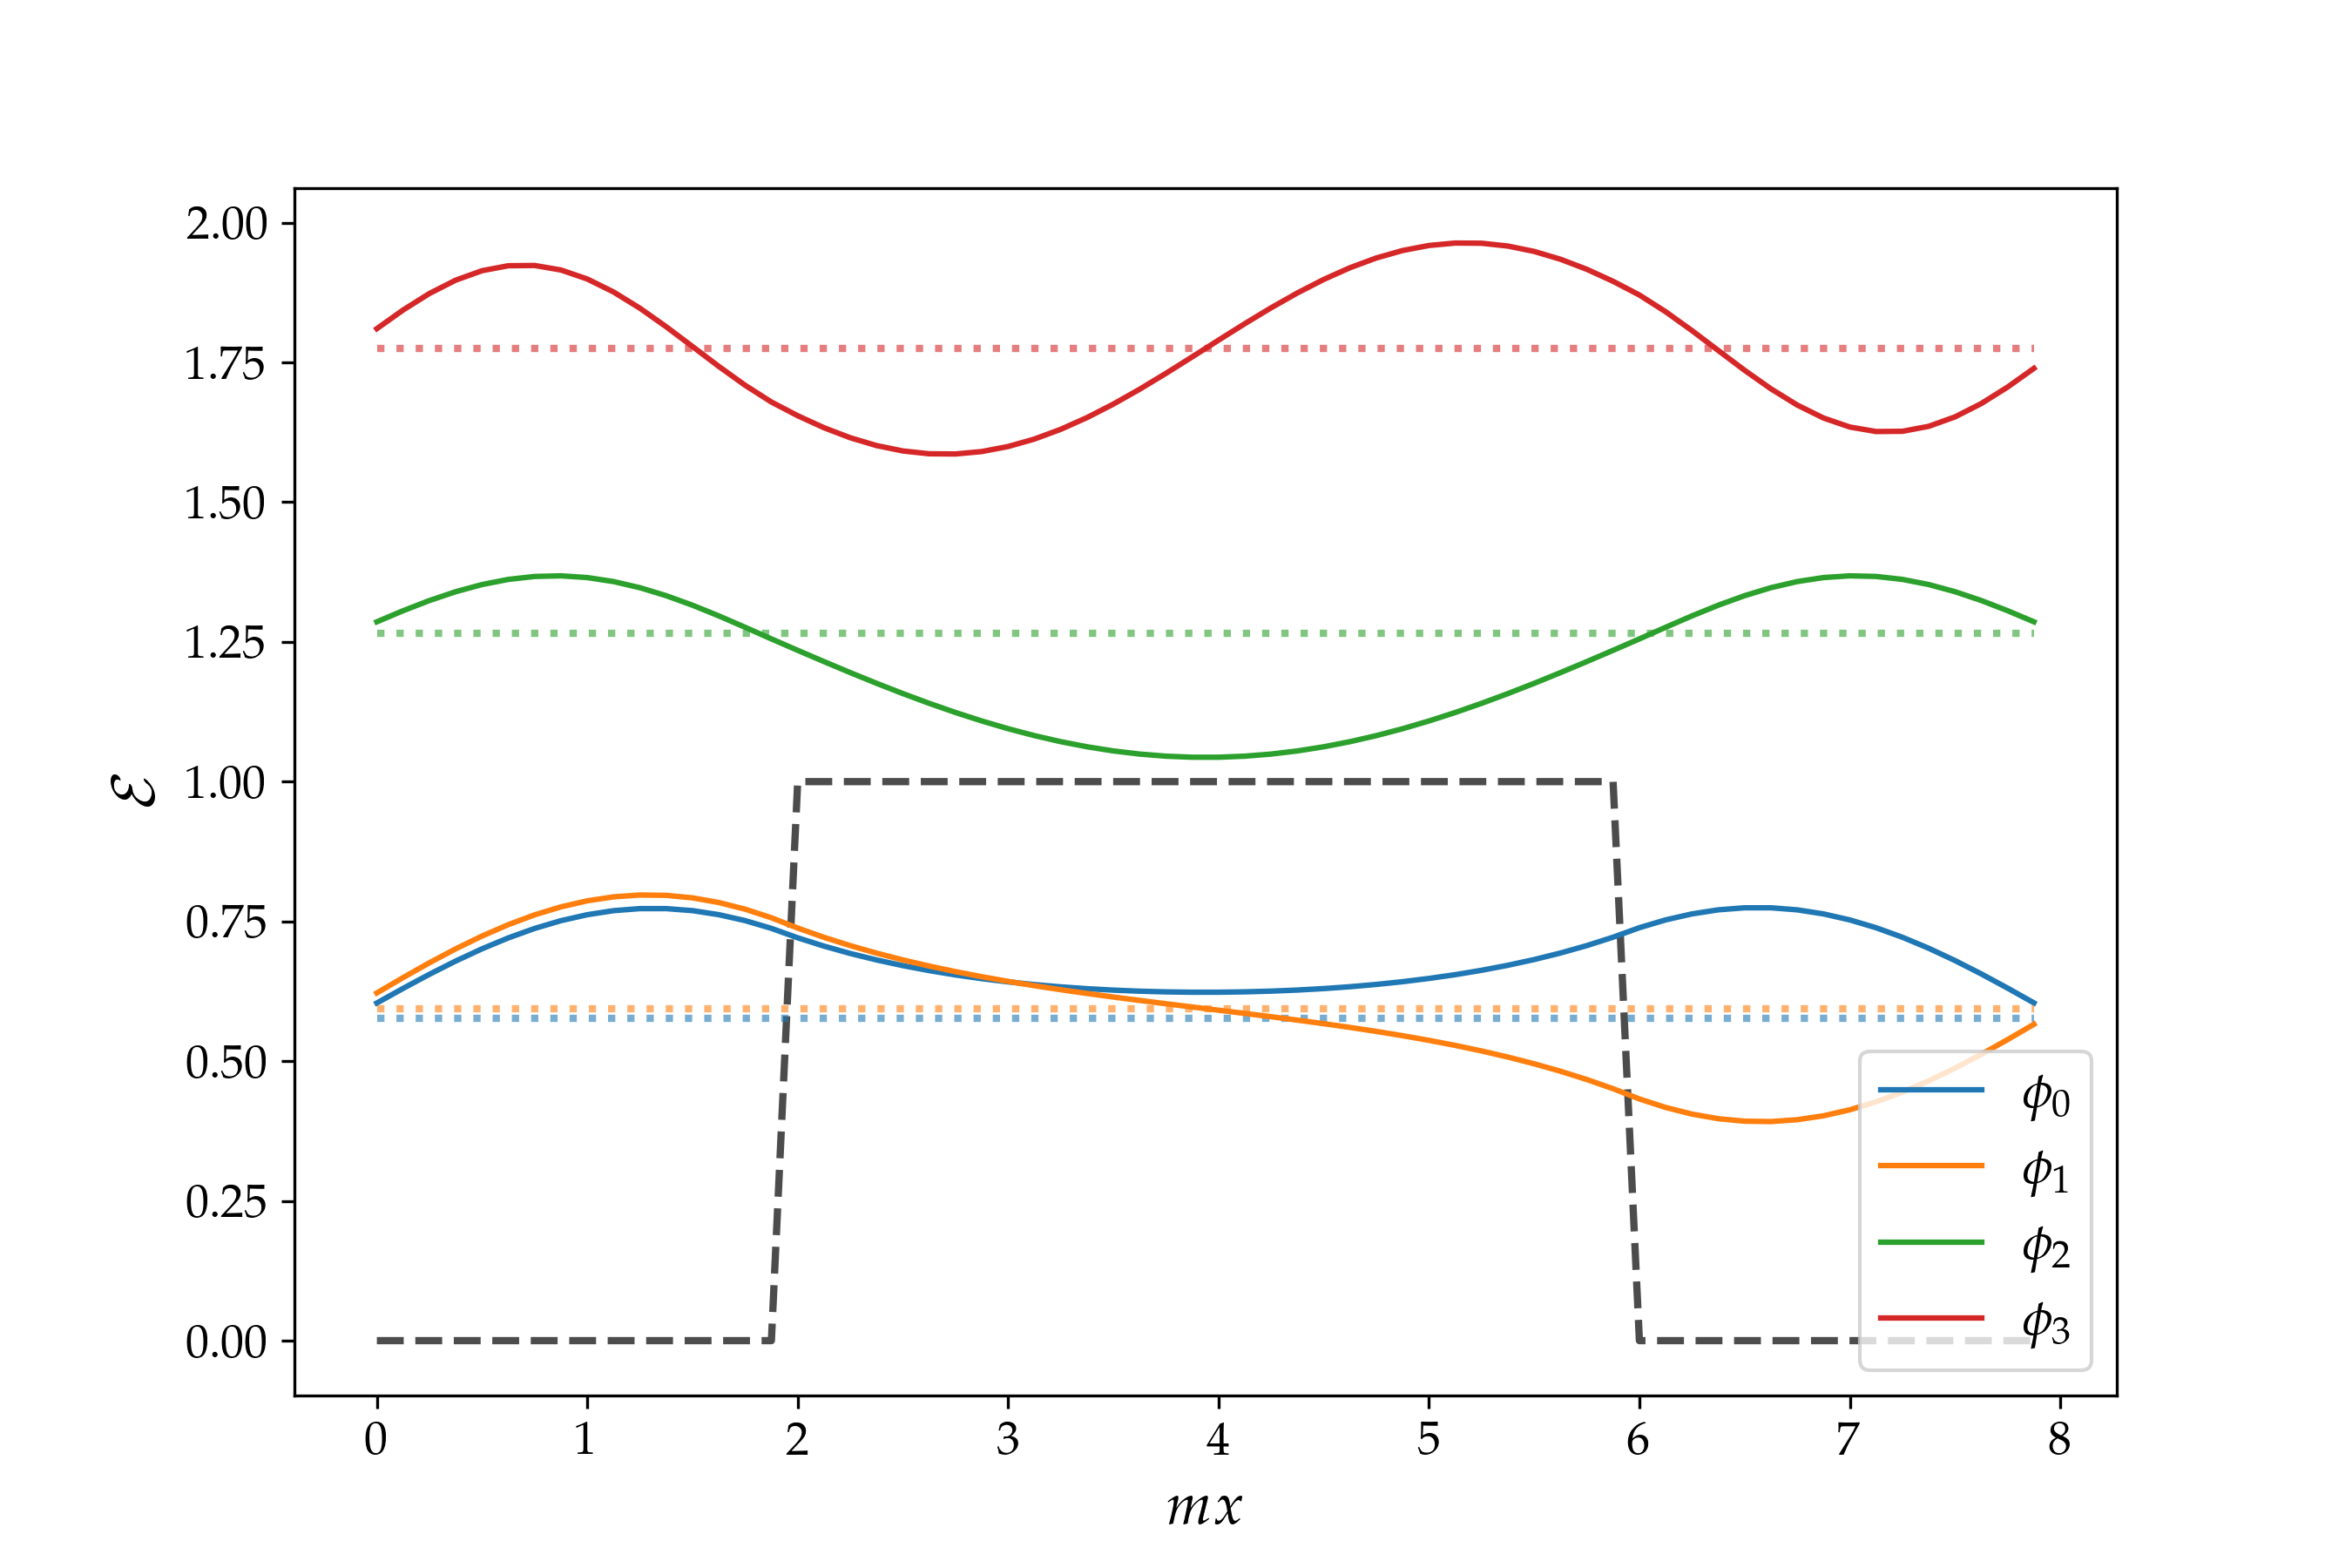
\includegraphics[width=0.7\linewidth]{images/18/finite_wall.png}
    \caption{I primi quattro autostati della barriera finita; si osserva una simil degenerazione per $\phi_0, \phi_1$.}
    \label{fig: fin_wall}
\end{figure}
\begin{figure}[H]
    \centering
    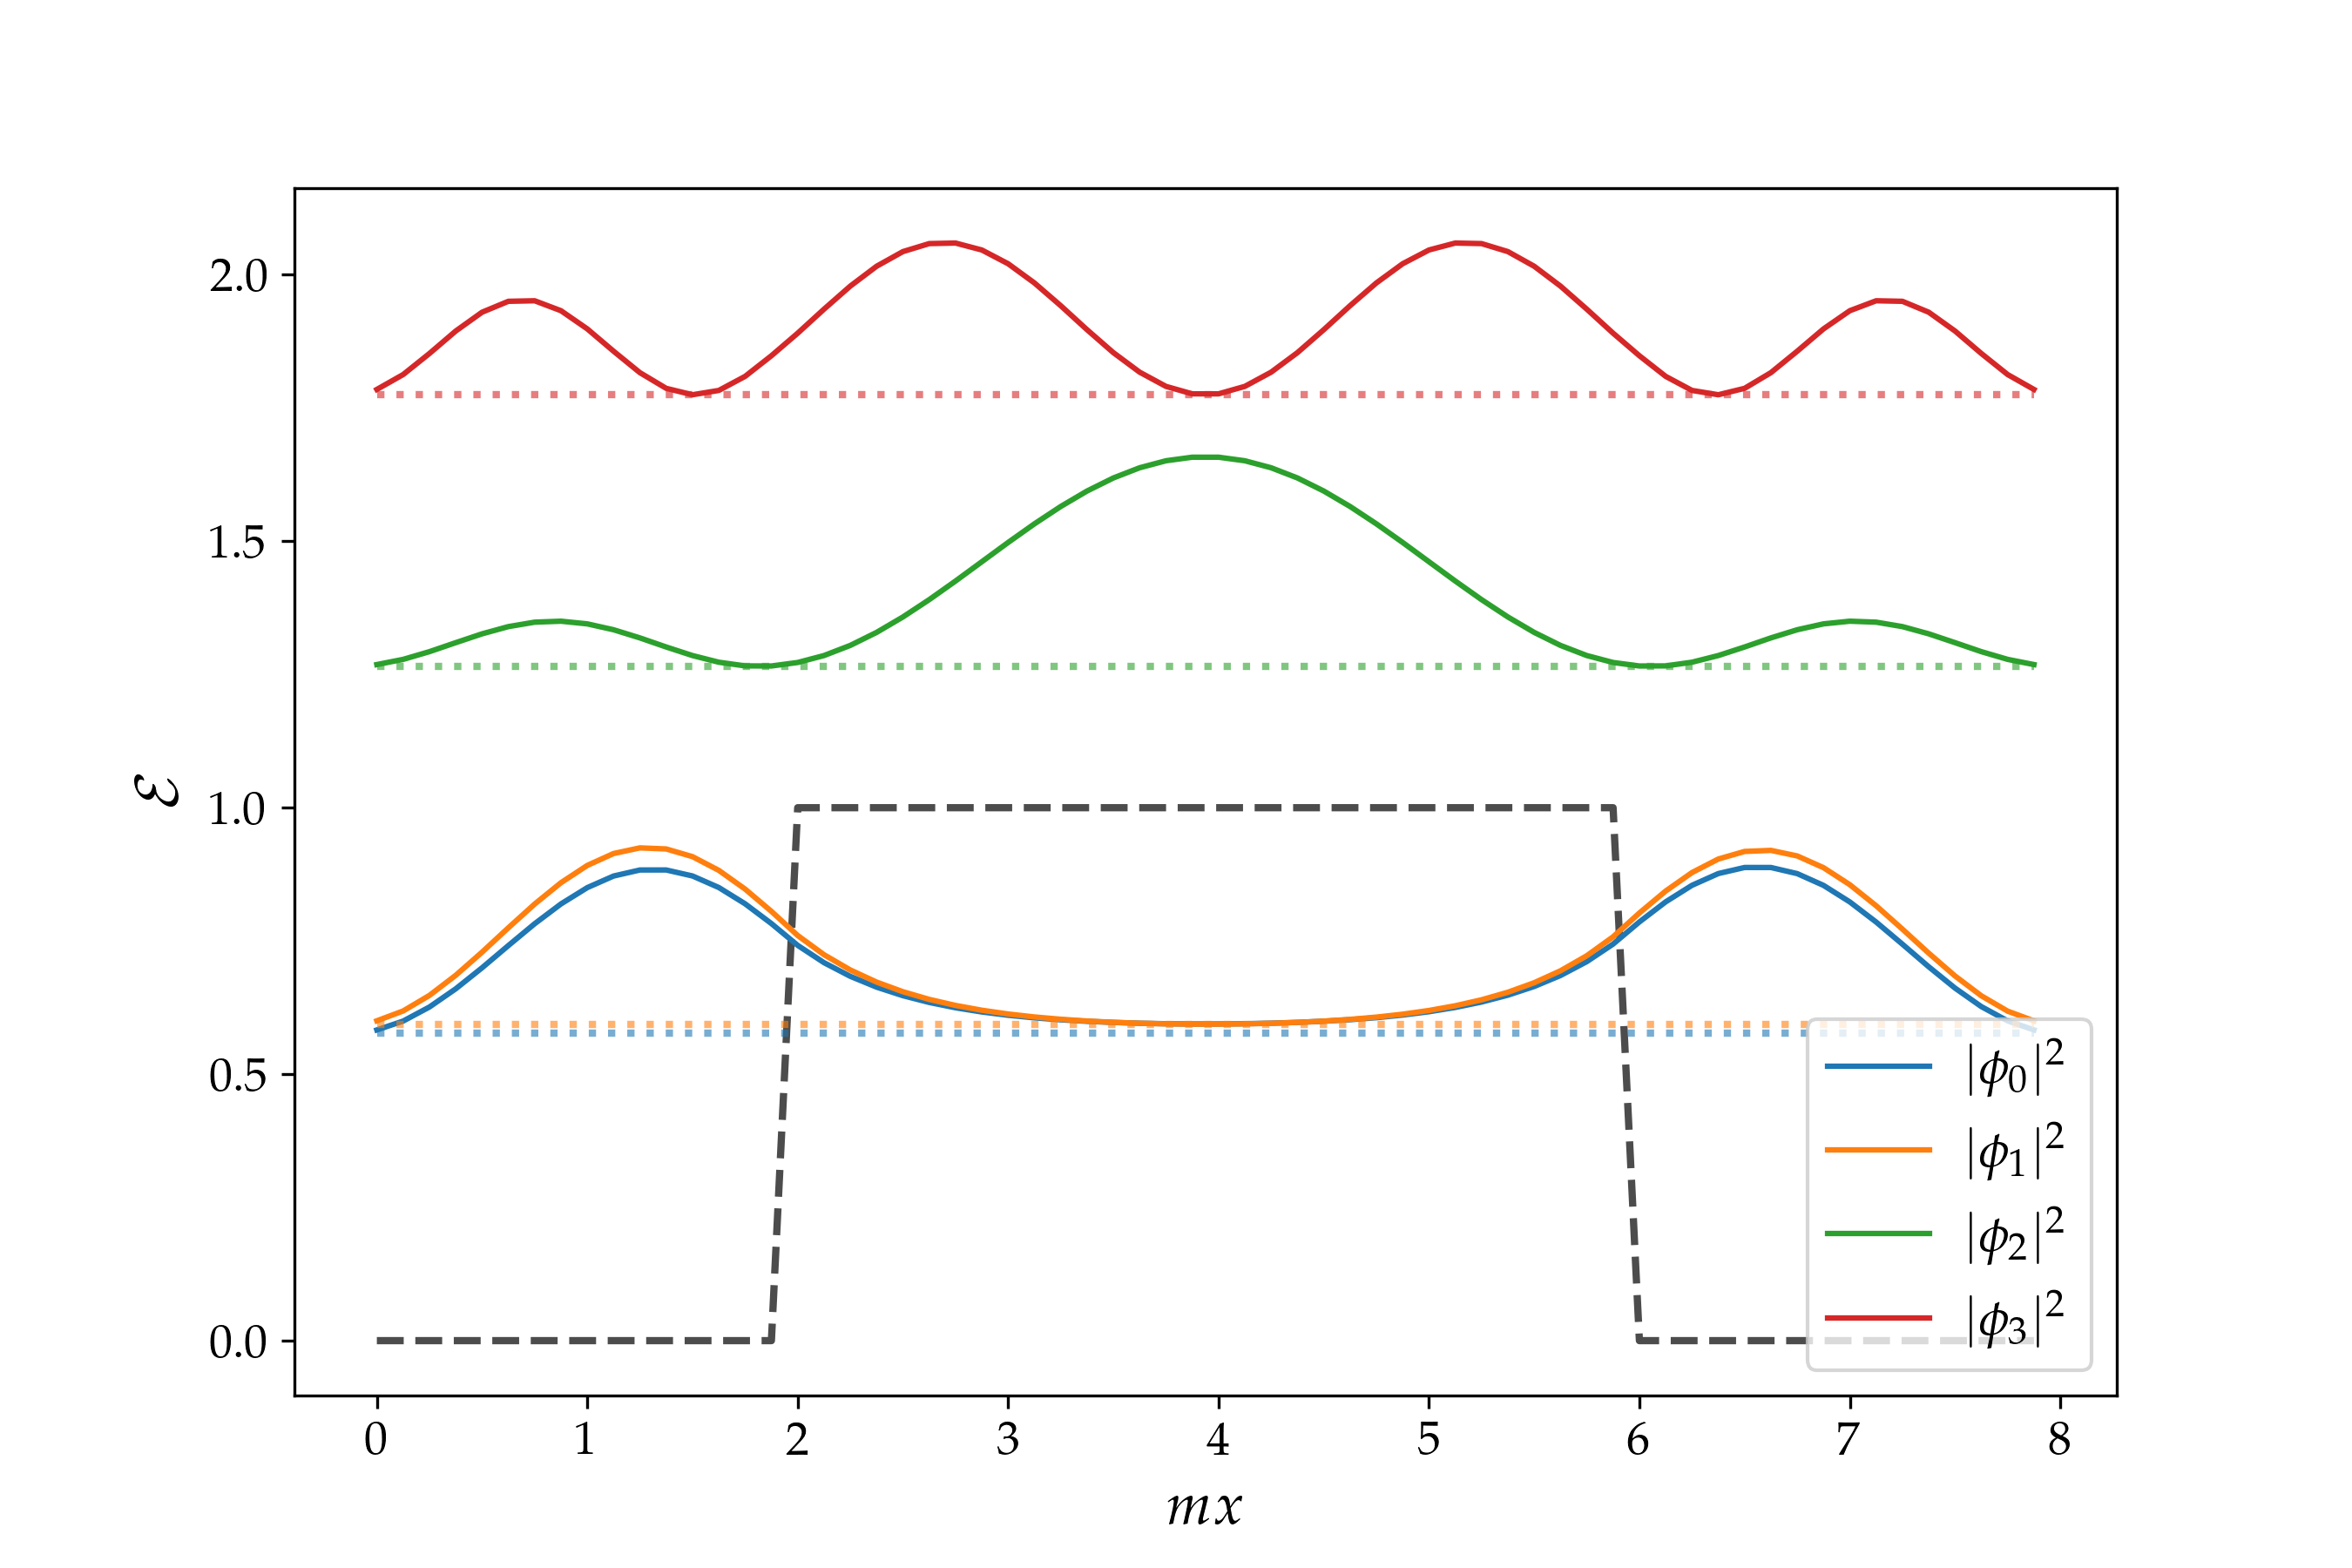
\includegraphics[width=0.7\linewidth]{images/18/finite_wall_mod2.png}
    \caption{Modulo quadro dei primi quattro autostati della barriera finita.}
    \label{fig: fin_wall_mod2}
\end{figure}




\subsubsection{Stati fondamentali al variare di $V_0/m$}
Tornando al caso della buca finita, studiamo cosa accade all'aumentare della profondita di questa: come si trasforma la funzione d'onda?\\
Quello che stiamo studiando è effettivamente l'approssimazione crescente a una buca infinita, la cui soluzione esatta è nota: gli autostati sono le funzioni
$$\psi_n(x) = \begin{cases} \sqrt{\frac{2}{b - a}} \sin\left(\frac{n\pi(x - a)}{b - a}\right) & a < x < b \\ 0 & \text{altrove} \end{cases}$$
\[
n=1,2,3, \dots
\]

di cui il \textit{GS}:
\[
\psi_{GS} = \sqrt{\frac{2}{b - a}} \sin\left(\frac{\pi(x - a)}{b - a}\right)
\]
dove il potenziale della buca infinita tra due estremi $a, b$ è definito come:
\[
V(x) = \begin{cases}
    0 & a<x<b\\
    +\infty & \text{altrove}
\end{cases}
\]

\noindent Concludiamo quindi che in Fig. \ref{fig: well_var} si osserva questa tendenza: si noti come diminuisca la profondità di perforazione della barriera nella regione proibita che la funzione d'onda riesce ad avere per via della decrescenza esponenziale sempre più rapida (che nel limite di barriera infinita fissa dei nodi nei punti $a, b$). 


\begin{figure}[H]
    \centering
    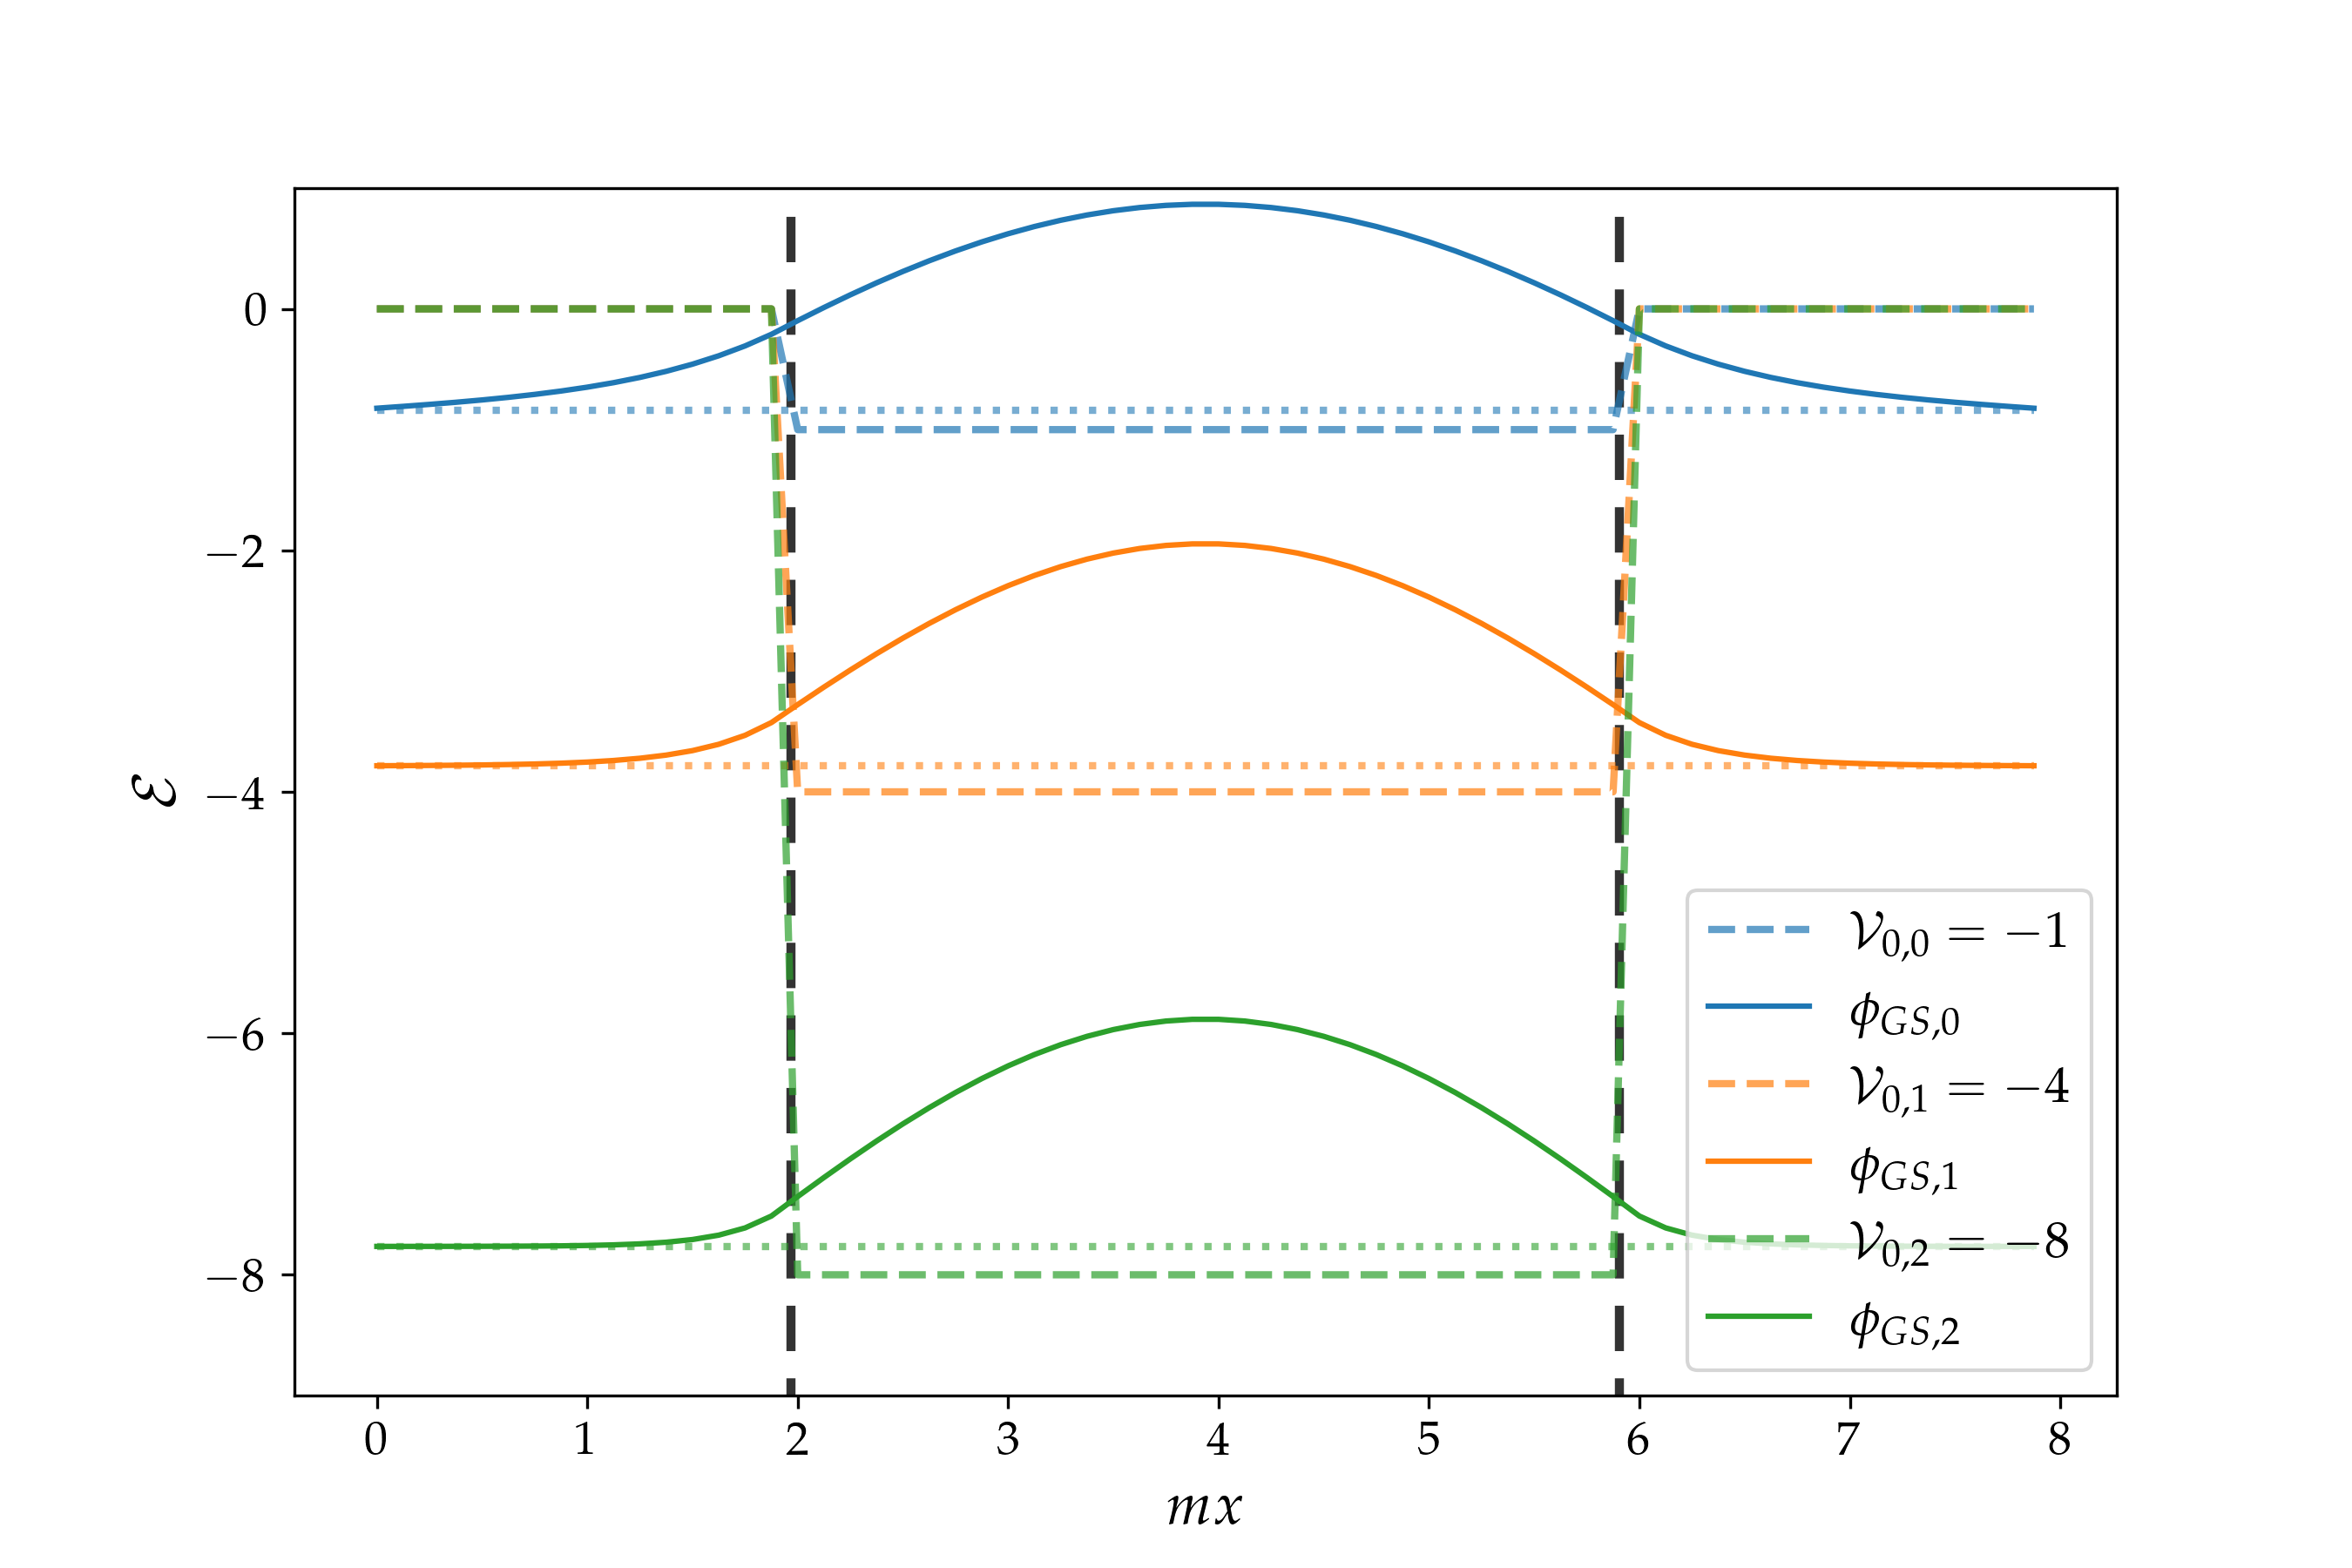
\includegraphics[width=0.8\linewidth]{images/18/diff_well.png}
    \caption{\textit{Ground states} della buca finita, con diversi valori di $V_0/m \in \{1, 4, 8\}$.}
    \label{fig: well_var}
\end{figure}

\subsubsection{Scaling degli autovalori in funzione di $N$}
Fissando un potenziale di riferimento (nel nostro caso la buca finita) e studiando l'andamento degli $i$-esimi autovalori in funzione della discretizzazione spaziale $N$, si osserva che la velocità di convergenza verso il valore esatto non è uniforme per tutti gli stati.
Per visualizzare meglio il fenomeno, in Fig. \ref{fig: scaling_eval N} abbiamo rappresentato gli autovalori normalizzati rispetto alla loro migliore approssimazione (quella relativa alla massima risoluzione, $\lambda_{64}$), facendo sì che tutti convergano asintoticamente a 1. 
Dal grafico emergono i seguenti comportamenti
\begin{itemize}
    \item Autovalori minori: l'approssimazione risulta sufficientemente accurata anche a basse risoluzioni (valori di $N$ piccoli).
    \item Autovalori maggiori (stati ad alta energia): un $N$ piccolo restituisce un'approssimazione scadente. Poiché $N$ definisce la densità del campionamento sul quale valutiamo la funzione e la sua derivata seconda (approssimata tramite differenze finite), le autofunzioni più energetiche richiedono un reticolo molto più fitto per essere modellate in modo corretto.
    \item Stato fondamentale ($\lambda_1$): costituisce un caso limite, in quanto si osserva che l'errore sul calcolo di questo autovalore si mantiene pressoché costante $\forall N$.
\end{itemize}


\begin{figure}[H]
    \centering
    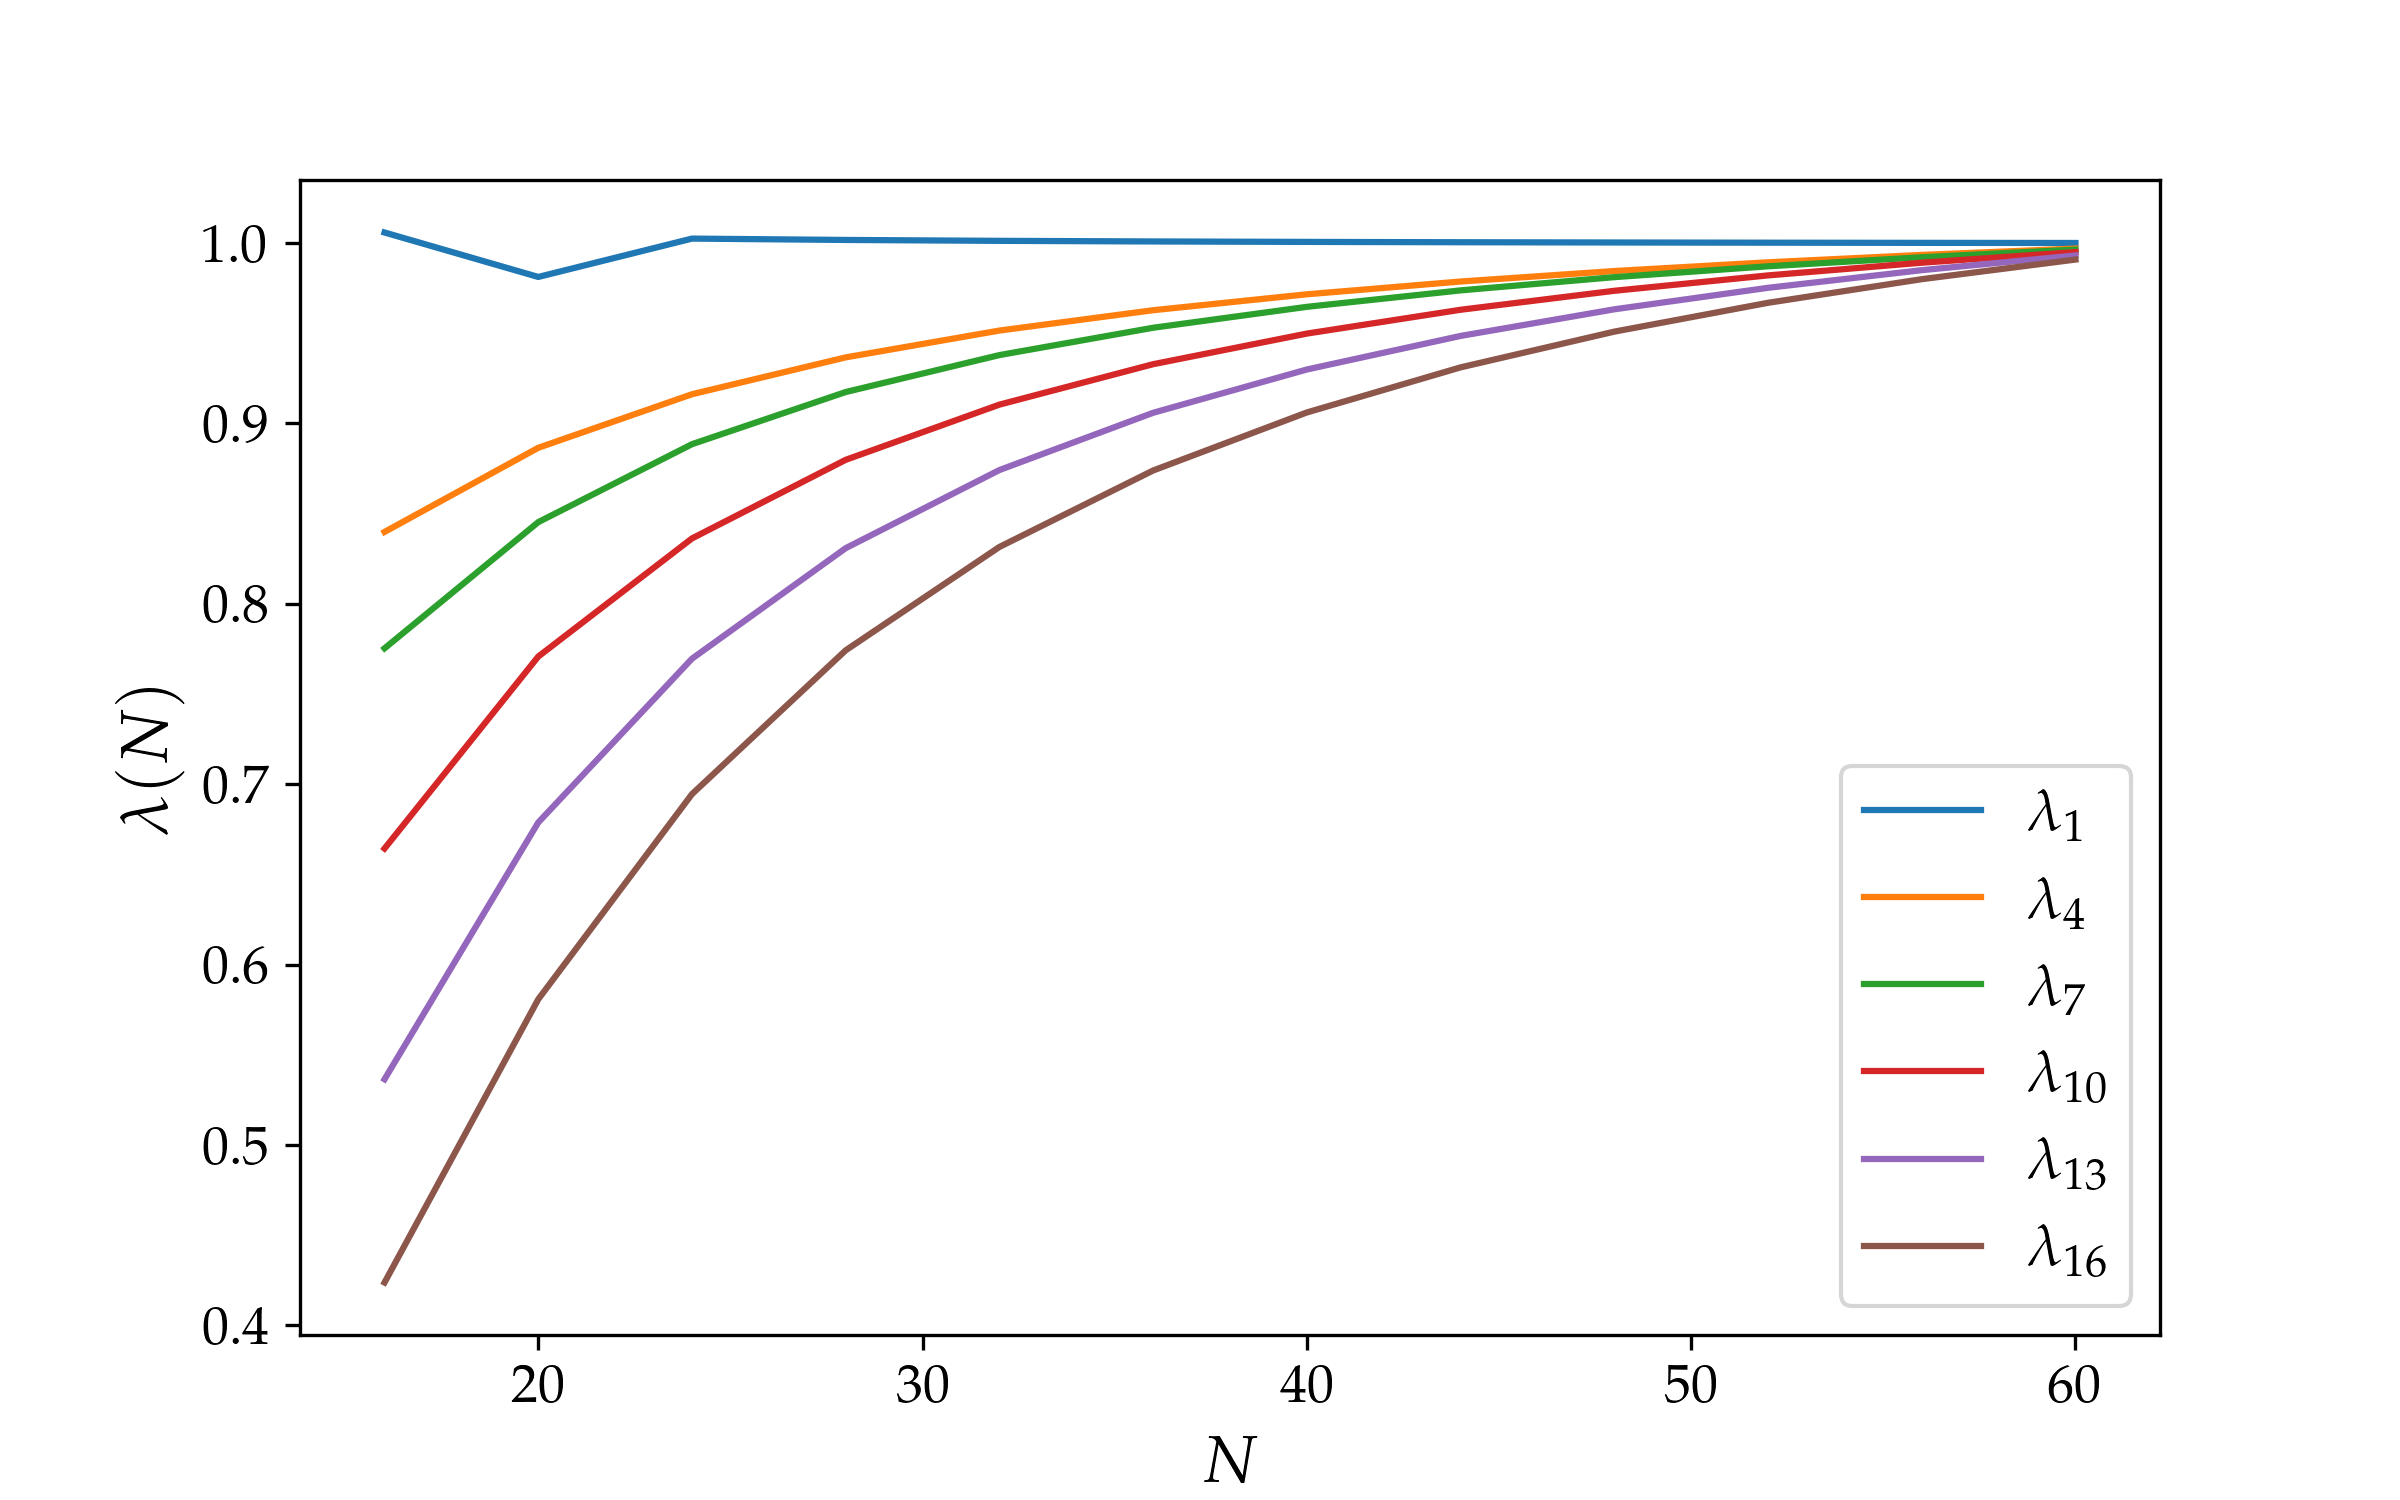
\includegraphics[width=0.8\linewidth]{images/18/rate_N.png}
    \caption{Rate di convergenza degli autovalori i-esimi in funzione di $N$.}
    \label{fig: scaling_eval N}
\end{figure}

\subsubsection{Soluzioni per diversi potenziali statici}
Infine desideriamo dare una breve descrizione del risultato che si può ottenere al variare della forma del potenziale. Delle considerazioni di interesse fisico possono essere fatte sulle soluzioni relative a questi potenziali, ma in questo caso lasciamo la semplice definizione dei potenziali, i loro parametri per i plot e la figura esplicativa Fig. \ref{fig: Diff Pot}.

\medskip\noindent
La buca finita è già stata discussa ampiamente nelle precedenti sezioni, la riproponiamo per il confronto con i casi adiacenti.

\medskip\noindent
La \textbf{buca doppia} è definita da:
$$V(x) = a x^4 - b x^2$$
nel mio codice in particolare applico una traslazione e una dilatazione:
$$x = \frac{u - \frac{N}{2}}{8},\ a=1/2 ,\ b=2$$

\medskip\noindent
Il \textbf{potenziale triangolare} è proprio di un campo di forza costante (per esempio il campo elettrico all'interno di un condensatore):
$$V(x) = \begin{cases} +\infty & \text{se } x < a \\ m \left(x - a\right) & \text{se } x \ge a
\end{cases}$$

i parametri sono stati impostati a:
\[
a=\frac{N}{4}, m = 0.3
\]

\medskip\noindent
Il \textbf{potenziale alfa} è invece quello relativo alle interazioni nucleari:
\begin{enumerate}
    \item Un pozzo attraente, derivato dalla forza nucleare forte a corto raggio, confina una particella poco energetica all'interno del nucleo
    \item Un potenziale coulombiano definisce una barriera respingente, ma che uno stato sufficientemente energetico può superare per tunneling quantistico. Questo fenomeno, descritto anche da Gamow, permette di descrivere per esempio l'emissione di particelle alfa energetiche.
\end{enumerate}

$$V(x) = \begin{cases} -V_0 & \text{se } x < R \\ \frac{k}{x - x_0} & \text{se } x \ge R \end{cases}$$

nel codice queste le impostazioni:
\[
R = \frac{N}{4}, k = 2, x_0=15
\]


\begin{figure}[H]
    \centering
    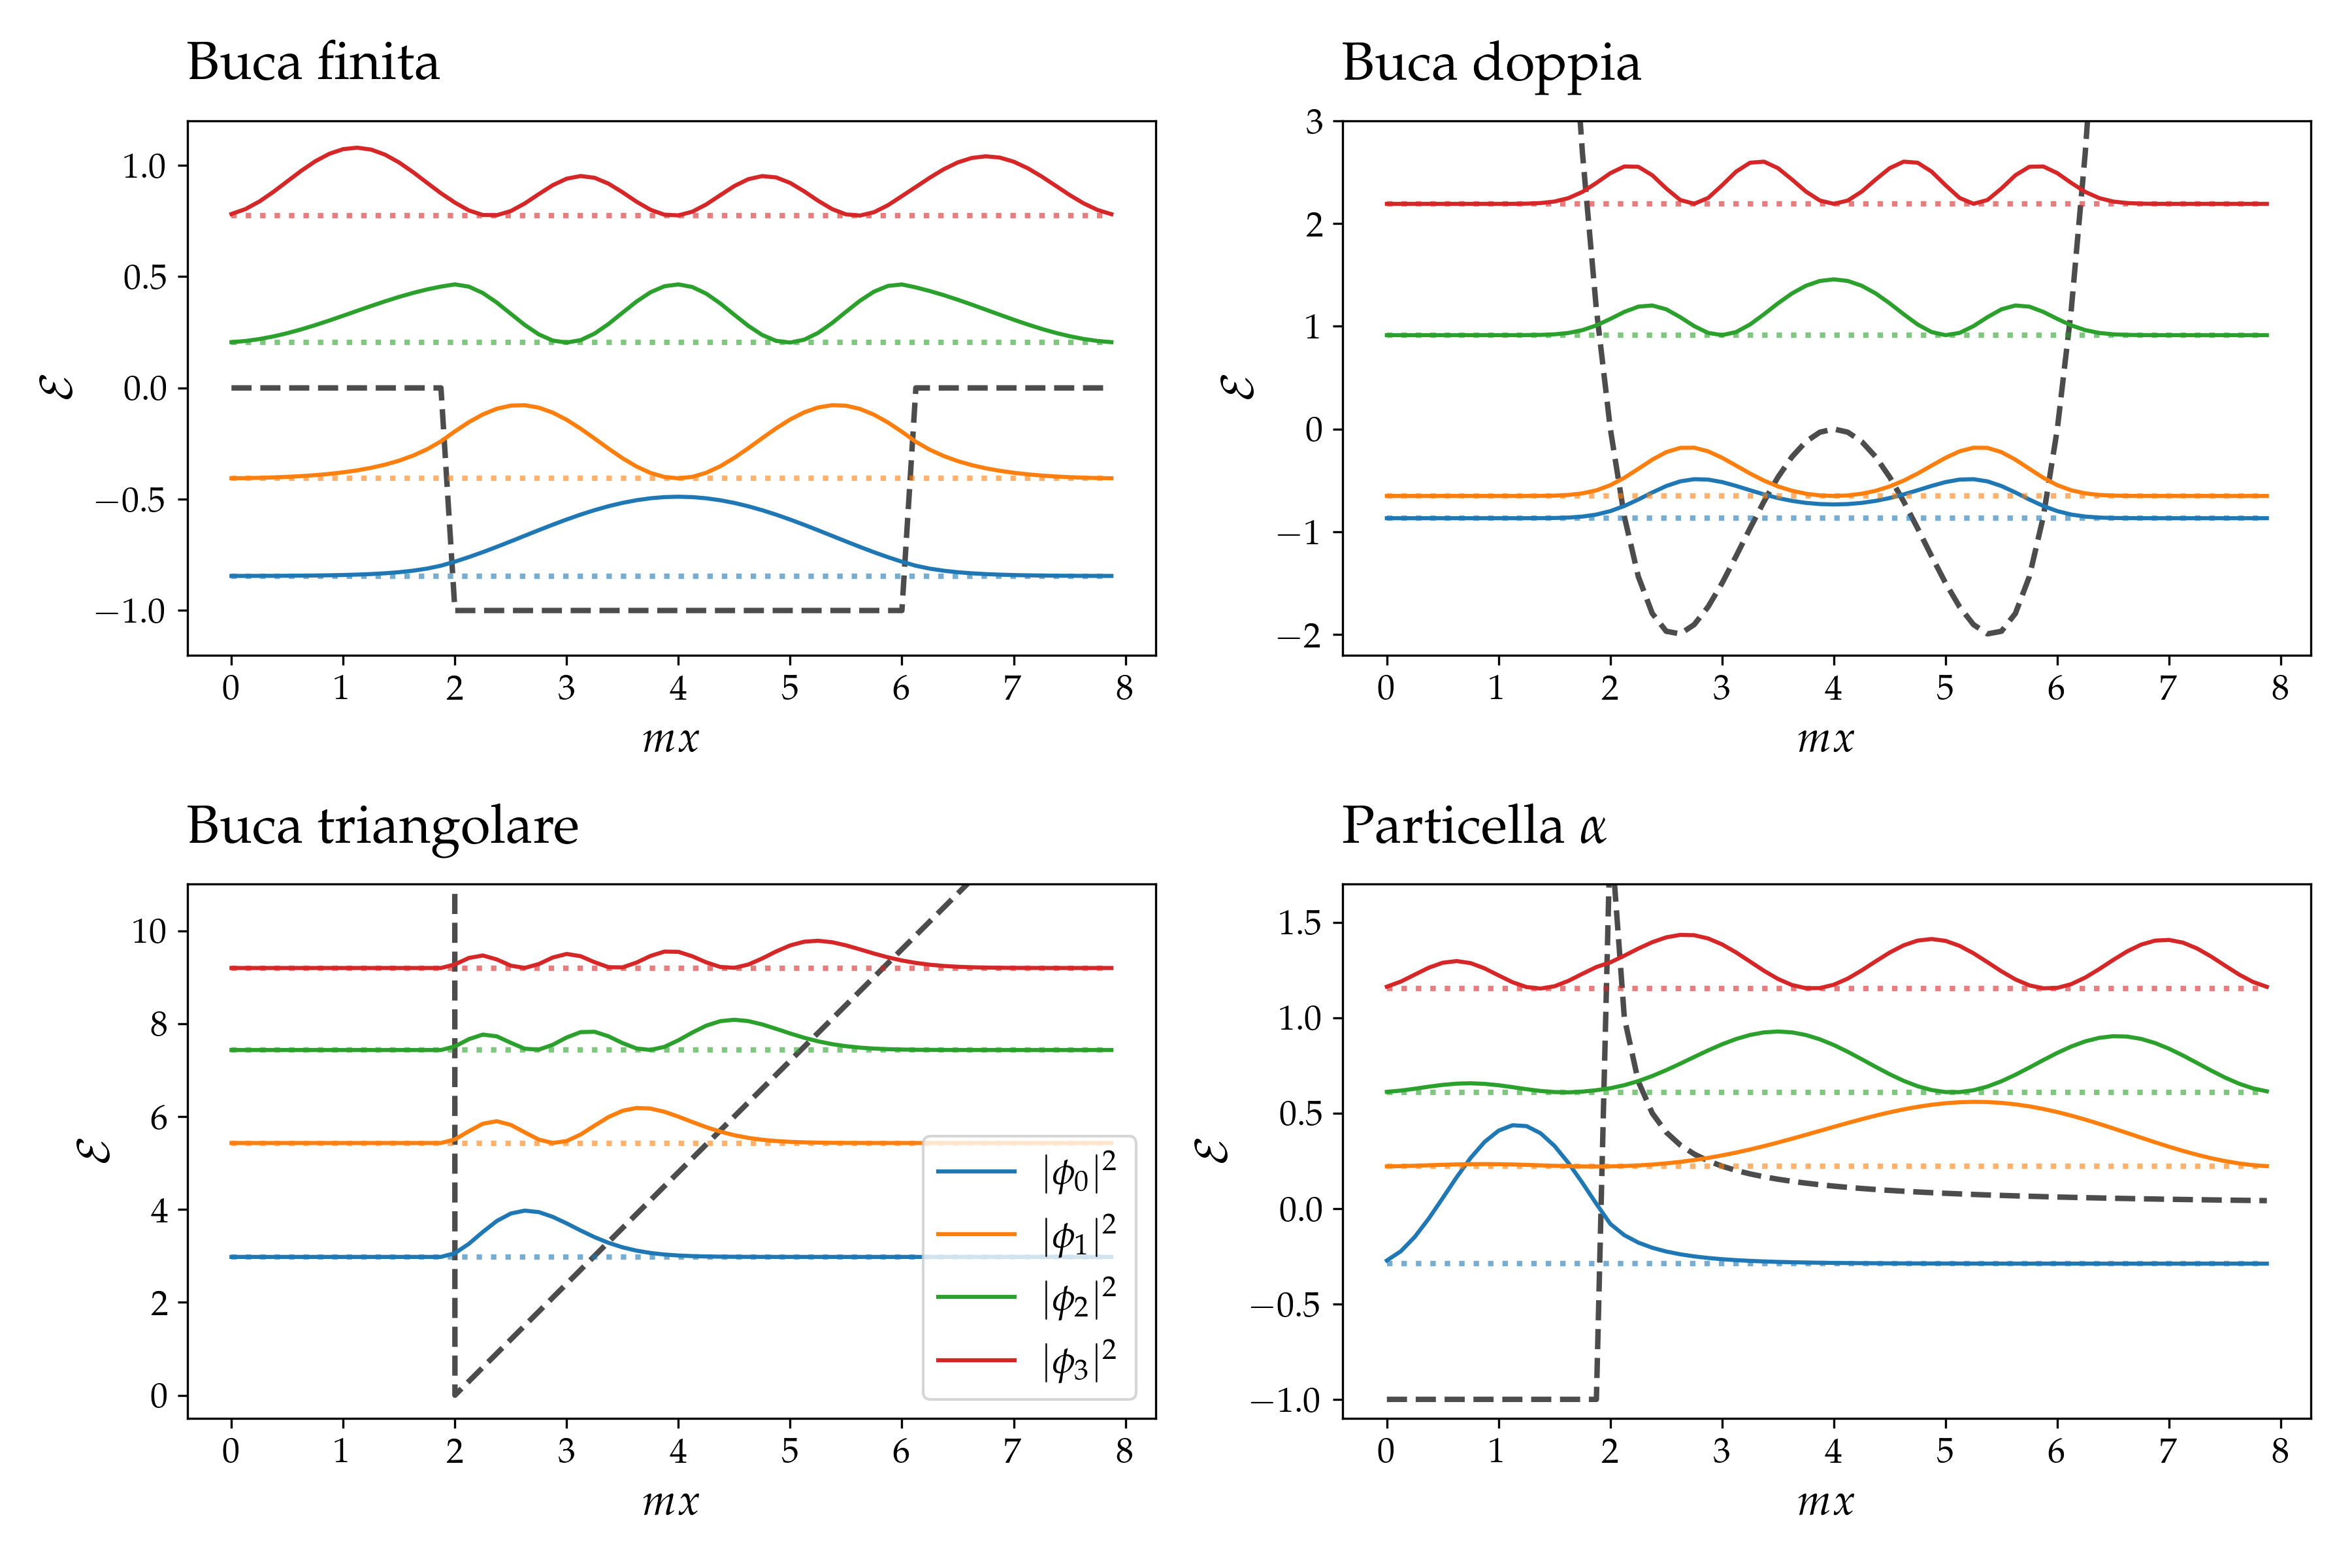
\includegraphics[width=\linewidth]{images/18/comp_Vs.png}
    \caption{Per differenti potenziali statici mostriamo il modulo quadro dei primi quattro autostati.\\
    Si osservi la quasi degenerazione nel grafico relativo alla \textit{double well}, simile a quella descritta nella sezione precedente: il sistema è ancora una volta una buca doppia, con una barriera di potenziale che la divide. Si presentano quindi gli stati quasi degeneri.}
    \label{fig: Diff Pot}
\end{figure}

\newpage














\section{Esercizio 7.2.1}



\subsection{Problem Statement}
Scrivi un programma che implementi lo schema RK4 per risolvere l'equazione di Schrödinger per un pacchetto d'onda incidente, situato in posizione $y$ al tempo iniziale $0$, con momento $p$:$$\psi(x,0) = \mathcal{N} \exp\left(-\frac{|x-y|^2}{\sigma^2}\right) e^{ip \cdot x}$$Normalizza il pacchetto d'onda all'unità.  Per semplicità, definisci un reticolo regolare con la stessa spaziatura per le direzioni $x$ e $y$, con $L_0 = L_1 = L$, $a_0 = a_1 = a$ e $N_0 = N_1 = N = 64$ (mentre sviluppi il codice usa un $N$ ancora più piccolo).  Utilizza i seguenti parametri fisici:
\begin{center}
    $mL = 8$, $y = (L/4, L/2)$, $\sigma m = 0.5$, $p = (p_0, 0)$, $p_0 L = (2\pi)6$.  
\end{center}

\noindent Risolvi l'equazione di Schrödinger fino a $\tau \simeq 0.6$ per i seguenti casi:  
\begin{itemize}
    \item \textbf{Pacchetto d'onda libero}: $V(x,t) = 0 \quad \forall x,t$.  
    
    \item \textbf{Effetto tunnel}: crea una parete lungo l'asse $y$ (perpendicolare alla direzione del moto) con spessore $a$ (o $2a$) situata al centro del reticolo, $L/2$, di ampiezza $32m$, ovvero:
    $$V(x,t) = \begin{cases} 32m & x_0 = [L/2, L/2+a], \forall x_1, t \\ 0 & \text{altrove} \end{cases}$$
    
    \item \textbf{Singola fenditura}: pratica un foro, centrato a $(L/2)$ e di dimensione $4a$, nella parete precedente.  
\end{itemize}
Studia l'evoluzione temporale tracciando $|\psi(x_0, x_1, t)|^2$ usando \textit{contour plots} a, per esempio, $mt = 0.0, 0.2, 0.4, 0.6$. Prova a realizzare anche un'animazione.\\
Per l'effetto tunnel considera di tracciare la norma della funzione d'onda lungo la direzione del moto (asse $x$), mentre per l'esperimento della singola fenditura tracciala a destra della fenditura, come se fosse uno schermo o un rivelatore.  

\subsection{Premessa Teorica}
Il problema si presenta come del tutto simile a quello precedente, però in particolare desideriamo andare a studiare l'evoluzione temporale del sistema, con la possibilità anche di introdurre potenziali non statici (dipendenti dal tempo).
Inoltre passiamo all'indagine di sistema bidimensionali, in cui possiamo effettivamente testare alcune configurazioni di reale approssimazione ad alcuni fenomeni fisici. 


\subsection{Metodi Numerici e Algoritmi}
Ci sono alcune caratteristiche che rendono questo esercizio diverso da quello del Cap. \ref{Cap. Schr t-indep}:
\begin{itemize}
    \item Si tratta di una discretizzazione su un reticolo 2D, quindi ci saranno due termini $a_i$ che determineranno questa risoluzione. Decidiamo di settare entrambi uguali.
    \item È necessaria la linearizzazione della funzione d'onda per la valutazione del laplaciano discretizzato: lavorando con una matrice di grande dimensioni l'operazione più dispendiosa diventa quella di conoscere il valore della fdo nei siti vicini. Con la programmazione in linguaggio \textit{python} è utilissimo l'aiuto della libreria \textit{numpy} che incorpora un metodo che ci permette proprio di traslare il vettore di una posizione (incorporando intrinsecamente le condizioni al contorno periodiche), consentendo la valutazione necessaria in forma vettoriale e ottimizzata computazionalmente.
    \item Se con l'equazione in forma \textit{t-independent} siamo riusciti a riscrivere il problema come una ricerca degli autovalori, in questo caso sarà necessario risolvere esplicitamente l'equazione differenziale ricorrendo ai metodi già studiati nei capitoli precedenti: il metodo più robusto è risultato essere quello di RK4, lo scegliamo quindi per la soluzione.\\
    Dopo aver portato in forma adimensionale tutta l'equazione, la soluzione, con l'ausilio di RK4, diventa:
    \begin{equation*}
    \psi(\vec x, t+\Delta \tau) = \psi(\vec x,t ) + \frac{\Delta \tau}{6} (\psi_1 + 2 \psi_2 +2 \psi_3 + \psi_4)(\vec x) + O(\Delta \tau^5)
    \end{equation*}
    \begin{align*}
        \psi_1(\vec x) & = -i H_m \psi(\vec x) \\
        \psi_2(\vec x) & = -i H_m \big[\psi(\vec x) + \psi_1(\vec x) \Delta \tau/2 \big] \\
        \psi_3(\vec x) & = -i H_m \big[\psi(\vec x) + \psi_2(\vec x) \Delta \tau/2 \big] \\
        \psi_4(\vec x) & = -i H_m \big[\psi(\vec x) + \psi_3(\vec x) \Delta \tau \big]
    \end{align*}
    
    che definisce l'i-esimo step temporale.\\
    Sarà utile assicurarsi che il nostro algoritmo RK4 sia in grado di lavorare con matrici, facendo evolvere tutti i punti contemporaneamente, poiché questa implementazione si traduce in un enorme e indispensabile vantaggio computazionale. 
\end{itemize}


\subsection{Risultati e Discussione}
In generale ho deciso di aumentare la definizione della griglia a $128\times128$, quindi anche alcuni altri parametri sono stati modificati per adeguarsi o per preferenze grafiche: nonostante queste scelte tutti gli esercizi sono stati svolti rigorosamente e presentano dei risultati coerenti e che mi propongo di mostrare qui di seguito.

\medskip\noindent
I parametri modificati sono:
\begin{align*}
    p_0L = (2\pi)20 , \tau =0.4
\end{align*}

\noindent I plot (statici) che si mostreranno di seguito sono fermoimmagini delle relative animazioni. Sono stati catturati come rappresentazioni della $\psi(x, y, t_i),\ t_i\in [0, \tau]$ combinati con il potenziale $V(x, y, t_i)$ (con una trasparenza del $50\%$). Queste figure danno una chiara immagine del fenomeno, ma hanno il difetto di essere disegnate senza mantenere la normalizzazione della \textit{colormap}: ogni plot ha rinormalizzato la scala di colori della \textit{heatmap} usando il valore massimo presente nella matrice in quell'istante, non è quindi possibile confrontare come si diffonda la distribuzione di probabilità totale (chiaramente normalizzata a 1 in ogni momento), poiché due colori uguali su plot diversi non rappresentano lo stesso valore della $\psi$. Per un potenziale statico invece questo tipo di discorso non vale, e chiaramente esso rimane uguale a sé stesso in ogni istante.

\medskip\noindent
Vi sono alcuni dettagli in più che riguardano le animazioni e i plot statici, ma ne discutiamo nell'Appendice \ref{App: rappr schr}: queste note sono importanti per chiarire alcune scelte nelle rappresentazioni e le principali differenze che sussistono tra le immagini che seguono e le animazioni riportate nella repo Github. Ritengo che questo discorso possa limitarsi ad un approfondimento e che si possa rilegare all'interesse del lettore, nonostante io reputi queste animazioni la parte più interessante e completa prodotta nell'intero corso. Anche per questa motivazione si conserva una discussione più chiara ad una sezione separata come quella in appendice.


\subsubsection{Particella libera $V(x)=0, \forall \boldsymbol x, t$}
La particella evolve sul reticolo come particella libera: mantiene la forma di gaussiana simmetrica lungo ciascun asse indipendentemente, ma non è più simmetrica nel piano, poiché la campana si allarga in maniera differente lungo le due direzioni (la sua curtosi diventa $k<3$).\\
Il principio di indeterminazione agisce in maniera chiarissima in questo caso, la precisione che avevamo nell'istante iniziale sulla posizione della particella sta diminuendo al passare dei secondi poiché essa si comporta come un'onda che si propaga nello spazio!

\begin{figure}[H]
    \centering
    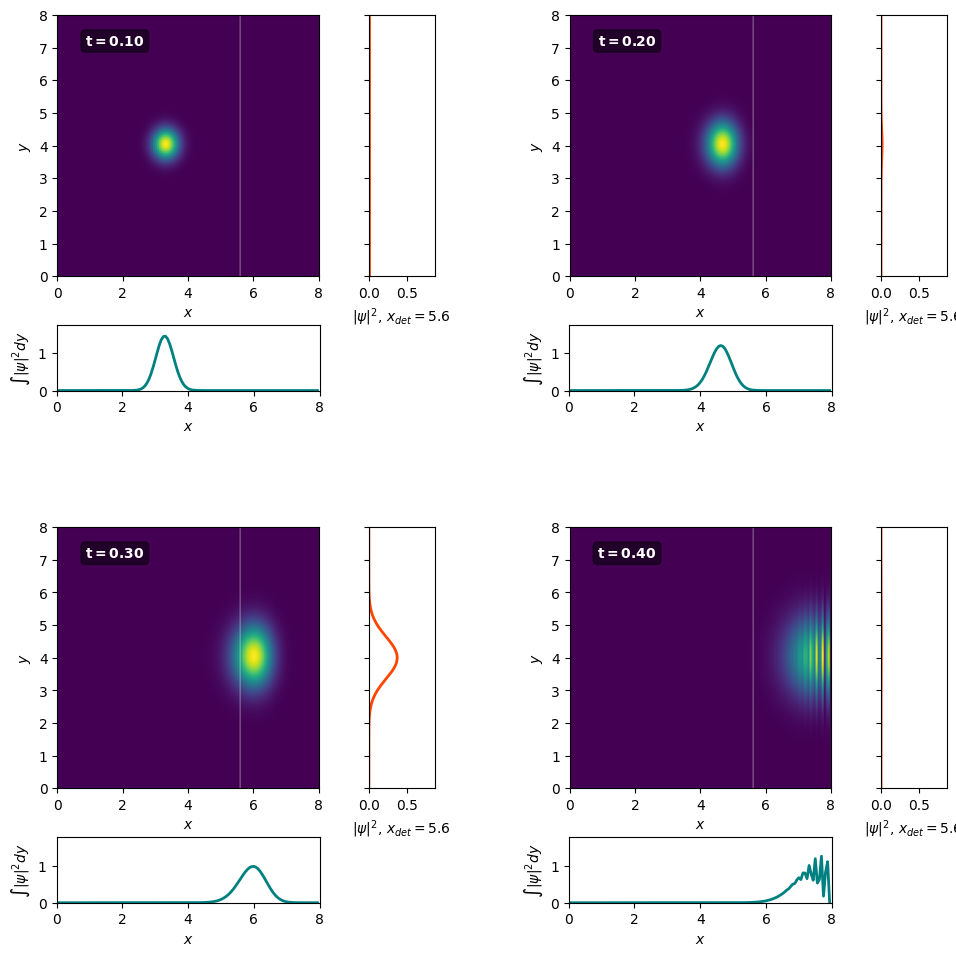
\includegraphics[width=0.8\linewidth]{images/19/pot/free_part_pot.png}
    \caption{Particella libera.}
    \label{fig: part_libera}
\end{figure}

\subsubsection{Effetto tunnel}
Per questo esempio prendiamo in considerazione una barriera di potenziale posizionata nel centro del dominio:
\begin{align*}
    V(x) = \begin{cases}
        V_0 \quad &x_{pos}\le x \le x_{pos} + d\\
        0 \quad &\text{altrimenti}
    \end{cases}    \quad \qquad\forall\ \boldsymbol y, t
\end{align*}

\noindent dove $x_{pos}$ è la posizione sull'asse x di questa barriera, mentre $d$ la profondità che abbiamo settato.\\
Ho impostato il livello $V_0$ del potenziale in maniera tale che ci fosse un buon equilibrio tra ciò che viene riflesso e quello che invece attraversa (tunneling); se il momento iniziale non è sufficiente, la particella verrà sempre più respinta dalla barriera, fino al punto che per lei sarà impossibile attraversarla perché nello spessore in cui abbiamo la regione proibita, dove $V(x)>E$, la funzione d'onda diventa evanescente e decade esponenzialmente, in maniera tale da confinare definitivamente la fdo nella regione a sinistra.  

\medskip\noindent
Il fenomeno è ben visibile in Fig. \ref{fig: bar_fin}.


\begin{figure}[H]
    \centering
    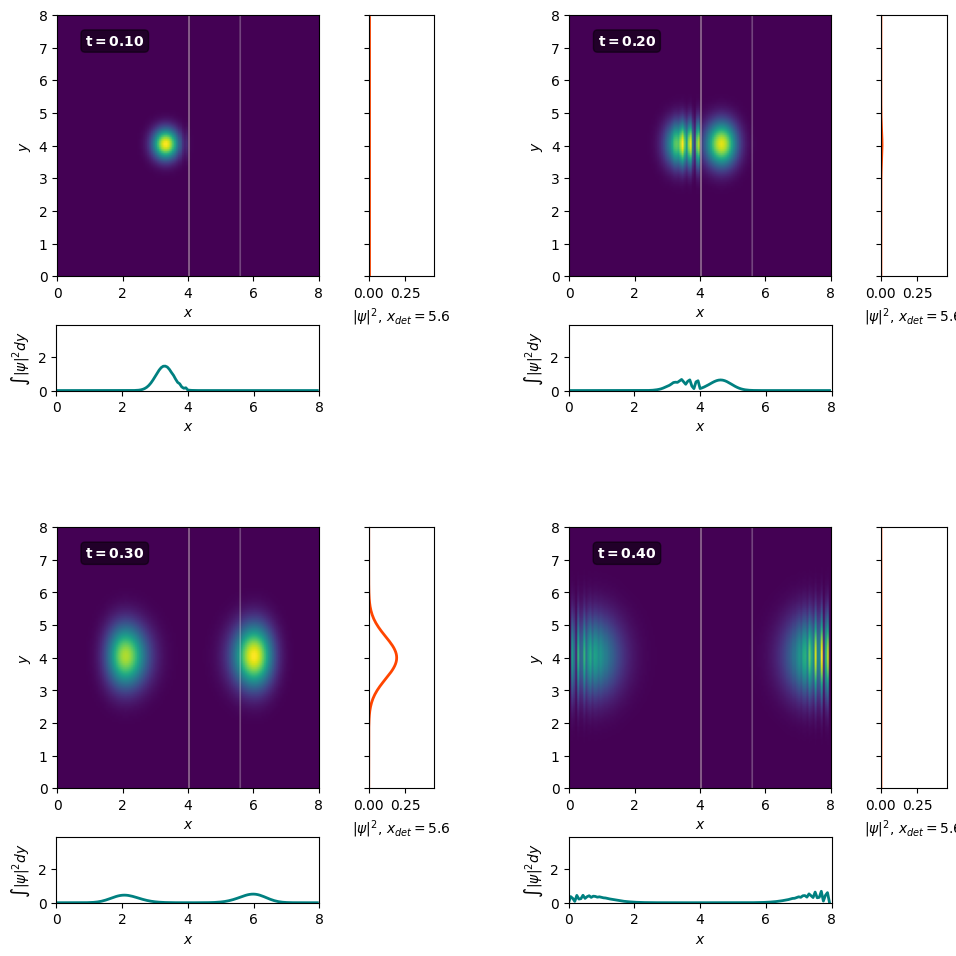
\includegraphics[width=0.8\linewidth]{images/19/pot/finite_wall_pot.png}
    \caption{Barriera finita e effetto tunnel.}
    \label{fig: bar_fin}
\end{figure}


\subsubsection{Singola (e doppia) fenditura}
Gli esperimenti con le fenditure sono il biglietto da visita per la QM, spesso il primo approccio con essa. In essi si può osservare direttamente e inequivocabilmente la natura ondulatoria della materia e si dà spiegazione di alcuni esperimenti particolarmente eclatanti.

\medskip\noindent
Quando un pacchetto d'onda interagisce con una barriera di potenziale infinita, osserviamo una riflessione totale dello stesso; se immaginiamo di forare questa barriera, permettendo quindi alla fdo di passare, si osserva il fenomeno di diffrazione, tipico di tutti i fenomeni ondulatori, e i relativi pattern di interferenza. Il plot che ho posizionato sulla destra, discusso in appendice, è un sensore, che risulta molto utile per simulare un esperimento di laboratorio e i possibili risultati che ci aspetteremmo di ritrovare su uno schermo.\\
In Fig. \ref{fig: one_slit} e \ref{fig: doub_slit} si osserva ciò che abbiamo discusso. La differenza fra i due fenomeni sta nel fatto che se nella singola fenditura ci si limita ad osservare la diffrazione, spiegata con il principio che ha una spiegazione nel principio di Huygens-Fresnel, cioè un fenomeno di autointerferenza, nella doppia fenditura questo si sovrappone all'interferenza che due sorgenti di diffrazione operano l'una sull'altra. Quello che si rileva è che per entrambi si generano figure di costruttive e distruttive, visibili come bande scure o chiare al di là della barriera. Si noti che la barriera di potenziale è impostata in maniera tale da essere sufficientemente energetica per essere considerata infinita; impostando valori ancora maggiori si osserva che il programma, nella sua operazione di risoluzione della PDE, si rompe, causando errori numerici e non conservando più la norma della fdo.

\begin{figure}[H]
    \centering
    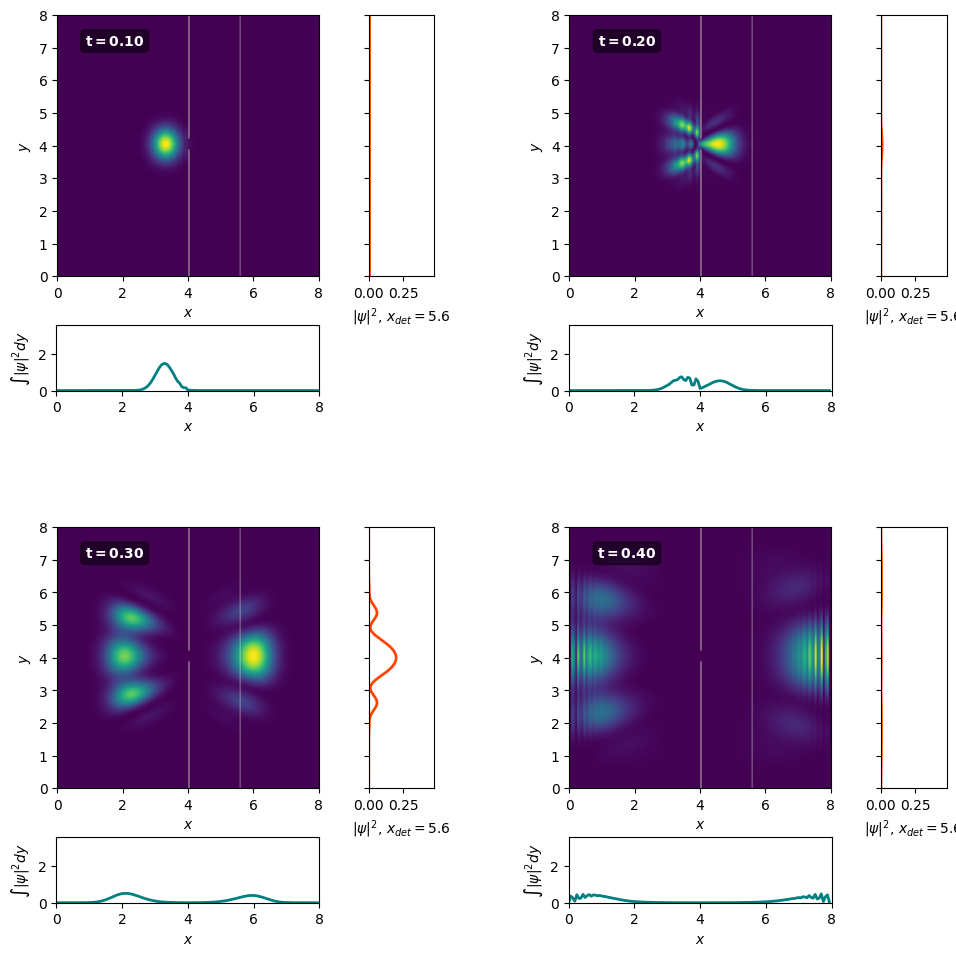
\includegraphics[width=0.65\linewidth]{images/19/pot/one_slit_pot.png}
    \caption{Esperimento a fenditura singola.}
    \label{fig: one_slit}
\end{figure}

\begin{figure}[H]
    \centering
    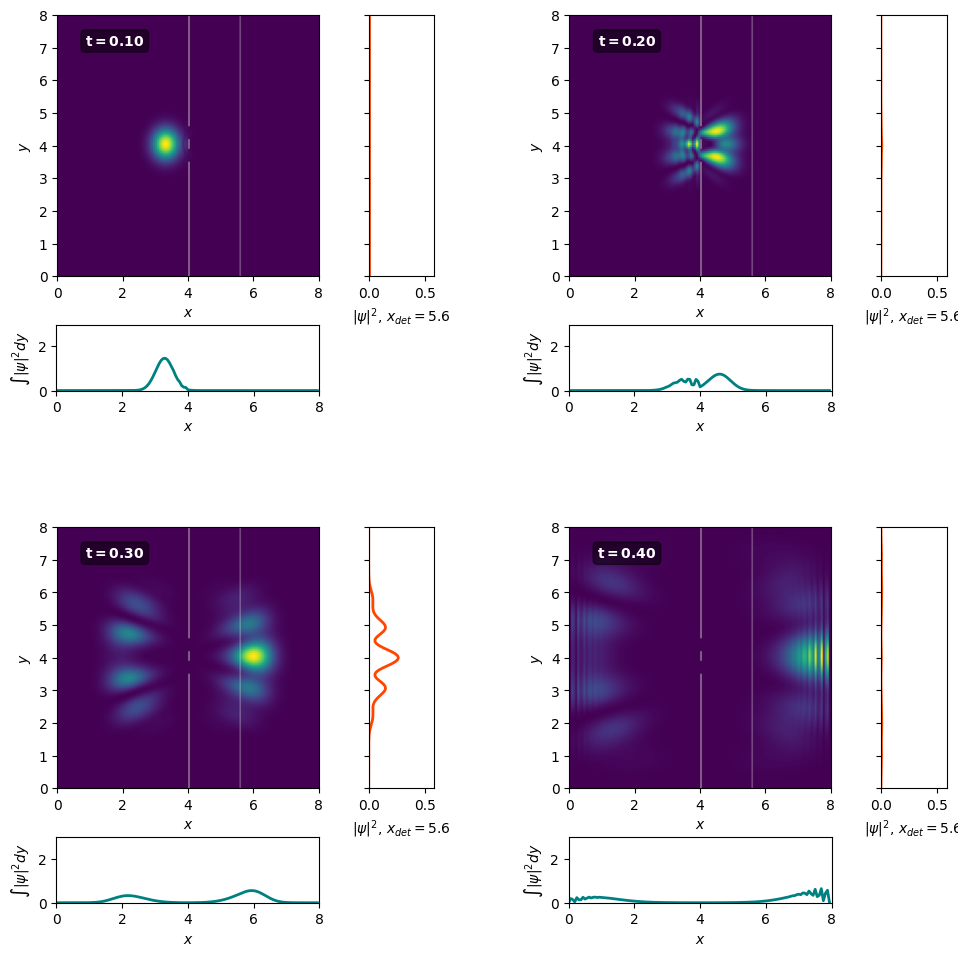
\includegraphics[width=0.65\linewidth]{images/19/pot/double_slit_pot.png}
    \caption{Esperimento della doppia fenditura.}
    \label{fig: doub_slit}
\end{figure}

\noindent Nello studio del fenomeno ho voluto sperimentare anche con altri casi che generalizzano i due precedenti: il reticolo di diffrazione e il singolo ostacolo.

Per quanto riguarda il reticolo di diffrazione esso è il caso n-esimo di diffrazione, con infinite, idealmente, sorgenti di onde sferiche, che sono le $n$ fenditure che si alternano costituendo il reticolo. Ciò che si rileva è la presenza delle fasce di interferenza, equivalenti a quelle delle esperienze già discusse.

L'ostacolo rappresenta un caso complementare alla singola fenditura: per il \textit{Principio di Babinet} essi provocano un fenomeno identico, andando a far interagire per interferenza l'onda incidente, in maniera però differente. Questo è il fenomeno osservabile con un ostacolo lineare sottile (un laser con un capello) oppure con un piccolo bersaglio circolare (si osservano i famosi \textit{Dischi di Airy}). 

\bigskip

\begin{figure}[H]
    \centering
    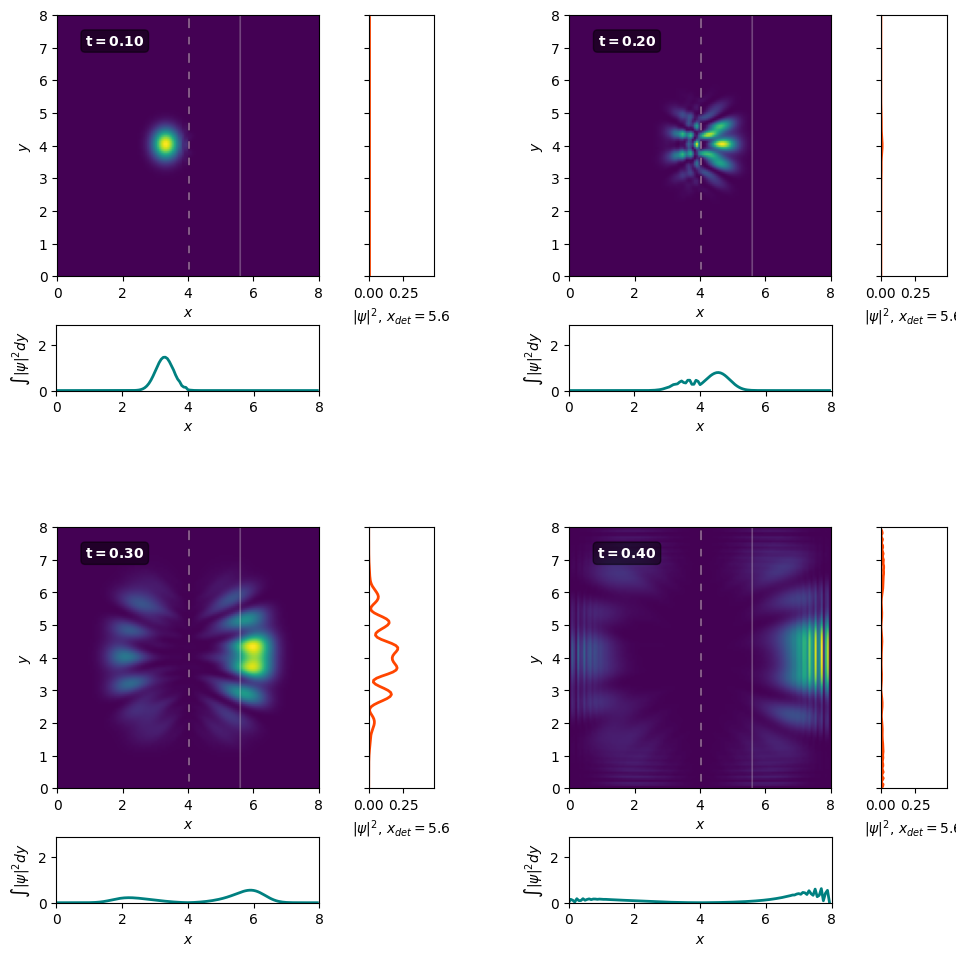
\includegraphics[width=0.7\linewidth]{images/19/pot/diff_grate_pot.png}
    \caption{Reticolo di diffrazione uniforme, ortogonale alla direzione di propagazione.}
    \label{fig: diff_grate}
\end{figure}


\begin{figure}[H]
    \centering
    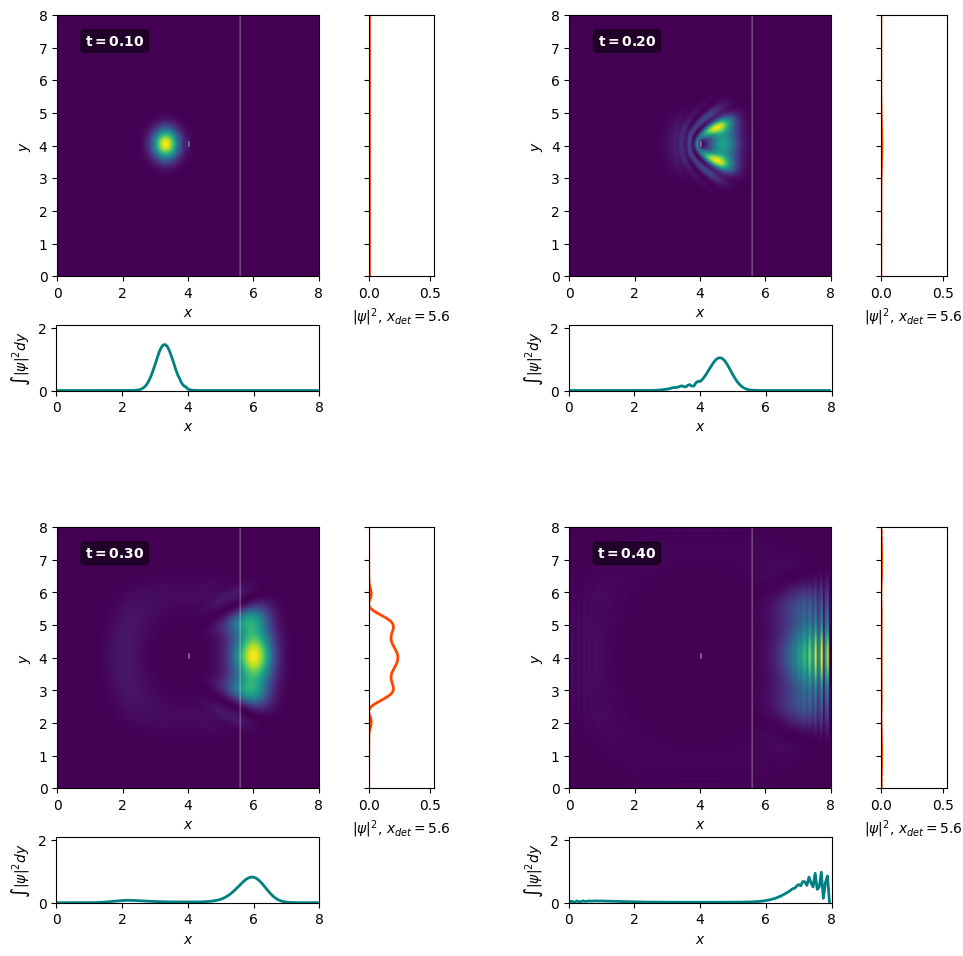
\includegraphics[width=0.7\linewidth]{images/19/pot/one_obst_pot.png}
    \caption{Diffrazione con un ostacolo.}
    \label{fig: diff_grate}
\end{figure}


\subsubsection{Casi di studio su potenziali alternativi}
Propongo in questa ultima sezione conclusiva alcuni casi di rilevanza fisica e che comunque presentano delle particolarità interessanti.

\bigskip

\noindent \textbf{Potenziale della particella alfa (\textit{Potenziale di Gamow}):}\\
\noindent Lo abbiamo già discusso nell'esercizio precedente; rimandiamo a quella sezione l'approfondimento generale. Proponiamo qui le soluzioni per un potenziale alfa configurato in due modi differenti: la barriera del potenziale coulombiano è più o meno intensa, risultando nella possibilità o meno di effetto tunnel e quindi esistenza di autostati esterni al nucleo (la particella alfa viene emessa e fugge), mantenendo il momento della particella uguale.\\
Nei grafici di seguito viene omessa la visualizzazione del potenziale, poiché è troppo opaco e non permette una chiara visibilità sul problema.

\begin{figure}[H]
    \centering
    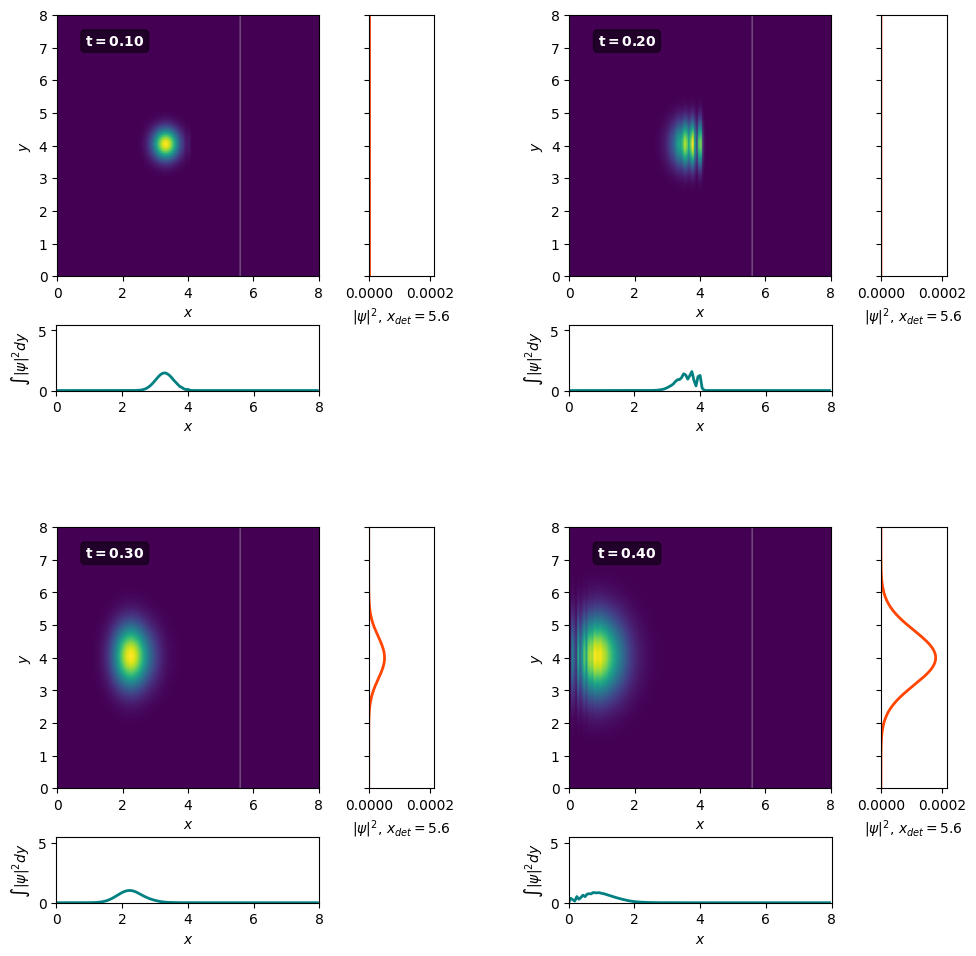
\includegraphics[width=0.65\linewidth]{images/19/no_pot/alpha_p_V0.png}
    \caption{Particella alfa confinata nella buca di potenziale (nucleo).}
    \label{fig:placeholder}
\end{figure}

\begin{figure}[H]
    \centering
    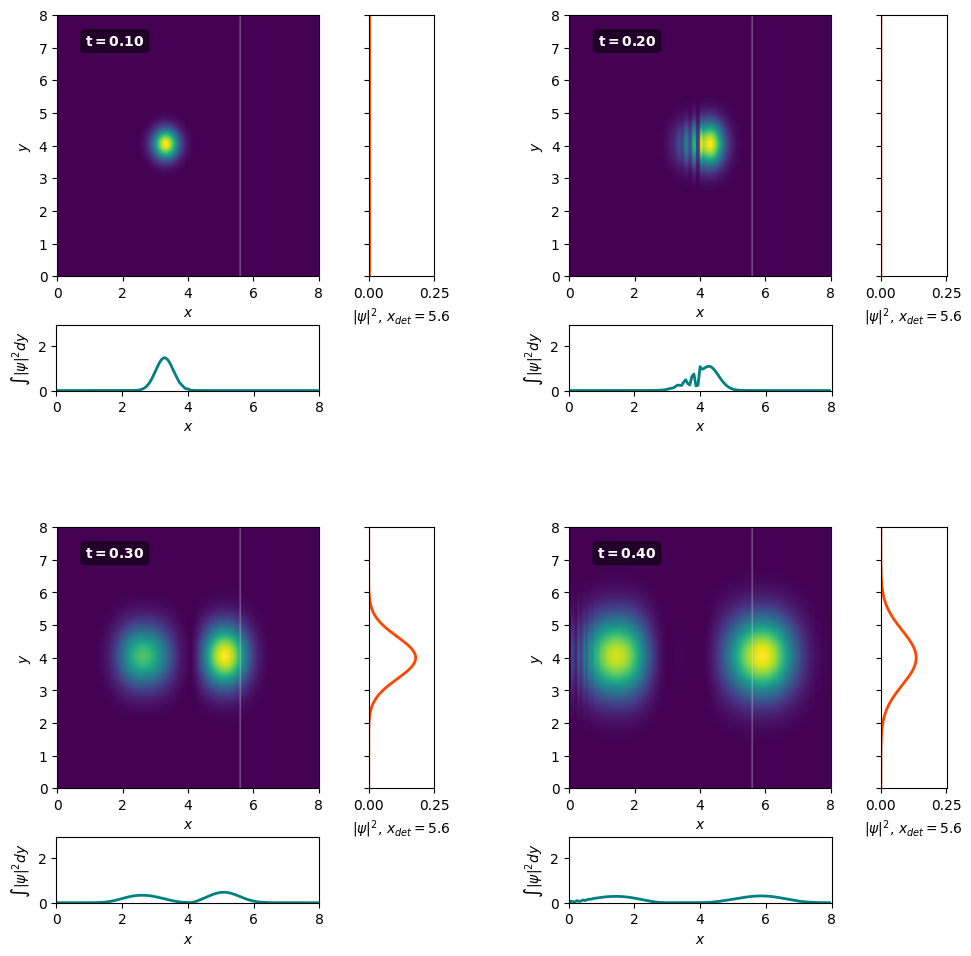
\includegraphics[width=0.65\linewidth]{images/19/no_pot/alpha_p_hV0.png}
    \caption{Particella alfa che riesce a fare tunneling e viene emessa dal nucleo.}
    \label{fig:placeholder}
\end{figure}


\noindent \textbf{Proiettile:}\\
\noindent Ho desiderato sperimentare anche con un potenziale variabile nel tempo introducendo un proiettile energetico che si muove nella stessa direzione e senso opposto rispetto al nostro pacchetto d'onda: si ottiene un urto frontale che distrugge l'integrità della campana gaussiana provocando, ancora una volta, dei pattern di interferenza. 

Questo non è un vero è proprio caso di potenziale \textit{t-dependent}, poiché a variare non è il valore $V_0$, bensì la localizzazione nel dominio, dell'ostacolo. Suppongo questo caso possa essere descritto come un esempio particolare di collisione con un ostacolo fermo di dimensioni analoghe, ma aumentando il momento $p_0$ della particella per combaciare con quello del moto relativo dei due.\\
Di seguito i risultati dell'analisi.

\bigskip

\begin{figure}[H]
    \centering
    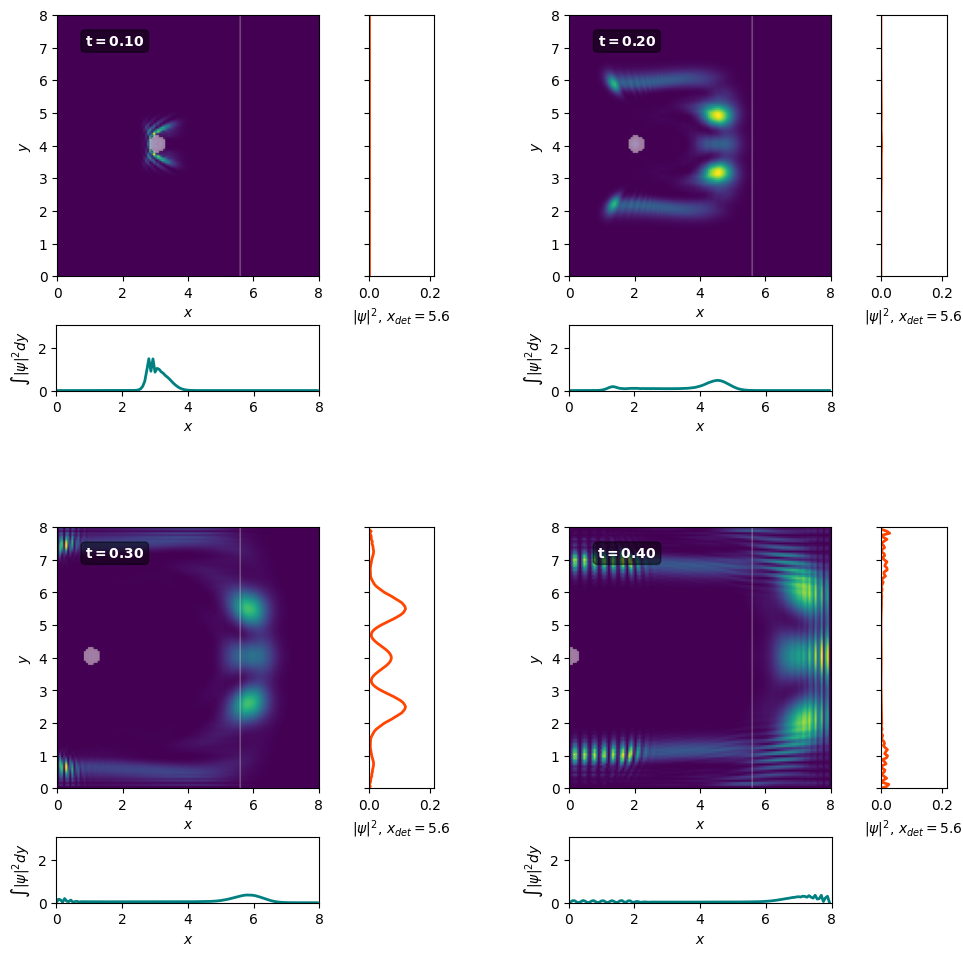
\includegraphics[width=0.8\linewidth]{images/19/pot/bullet_pot.png}
    \caption{Proiettile sferico di potenziale.}
    \label{fig: bullet}
\end{figure}



\newpage






\newpage
% \thispagestyle{empty} 
\null 
\clearpage

% --- PARTE 8: Integrazione numerica ---
\cleardoublepage 
\addtocontents{toc}{\bigskip\noindent\protect\textbf{\Large Integrazione numerica}\par\smallskip}
\addtocontents{toc}{\protect\setcounter{tocdepth}{-2}} 
\part{\Huge Integrazione numerica}
\addtocontents{toc}{\protect\setcounter{tocdepth}{2}} 


\section{Esercizio 8.1.1}
\subsection{Problem Statement}
Scrivere un programma che implementi sia la regola del trapezio che la regola di Simpson. Il programma dovrebbe essere in grado di accettare come dati di input l'intervallo $[a, b]$ e la spaziatura della griglia o il numero di sotto-intervalli.

\noindent Risolvere l'integrale

\[
\int_{x_0}^{x_0+\delta x} \sin^2(x/2) \, dx
\]

\noindent utilizzando un singolo intervallo in $[x_0, x_0 + \delta x]$. Verificare la scalabilità con $\delta x$ dell'errore della soluzione numerica confrontandola con quella analitica, $F(x_0 + \delta x) - F(x_0)$.

\subsection{Premessa Teorica}
Per valutare numericamente il valore dell'integrale definito di una determinata funzione $f(x)$, possiamo introdurre alcuni metodi che mostrano diversi approcci al problema. In particolare in questo esercizio studiamo i risultati di due diverse approssimazioni per interpolazione degli estremi di valutazione.

\subsection{Metodi Numerici e Algoritmi}
Il primo algoritmo risulta essere il più immediato: dato un intervallo infinitesimo (piccolo) $[x, x+\delta x]$, $\delta x \sim 0$, la curva può essere stimata con un'interpolazione lineare tra i due punti.\\
Si verifica che il risultato di questo metodo, denominato \textit{Regola dei trapezi}, sia:
\begin{equation*}
    \int_x^{x+\delta x} d\xi \, f(\xi) = \frac{\delta x}{2} \big[f(x) + f(x+\delta x) \big] + O(\delta x^3)
\end{equation*}

\medskip\noindent
Per generalizzare al caso di un intervallo esteso, può essere introdotta la \textit{Regola dei trapezi composta} come:
\[
\int_a^b dx \, f(x) = \frac{\Delta x}{2} \big[f(a) + 2 \sum_{i=1}^{N-1} f(a+i \Delta x) + f(b) \big] + O(\Delta x^2)
\]

\indent L’errore locale della regola del trapezio è $O(\delta x^3)$; nella versione composta l’errore globale è $O(\Delta x^2)$.

\bigskip\noindent
Una seconda possibilità è quella di lavorare con l'idea di migliorare questo primo algoritmo modificando la legge di interpolazione che scegliamo per l'approssimazione: in particolare scegliamo un'interpolazione quadratica. Sarà necessario valutare la funzione in tre punti per questa nuova scelta, ergo, per la definizione locale del metodo definiamo l'algoritmo sull'intervallo infinitesimo $[x, x+\delta x]$: si verifica che

\begin{equation*}
    \int_x^{x+ \delta x} d\xi \, f(\xi) \approx \frac{\delta x}{6} \big[f(x) + 4 f(x + \delta x/2) + f(x+\delta x) \big]
\end{equation*}
\indent La convergenza è di ordine 5 ($\sim \delta x^5$)\\

\noindent La regola composta può essere definita come:
\[
    \int_a^b dx \, f(x) \approx \frac{\Delta x}{3} \left[ f(a) + 2 \sum_{i=1}^{N/2-1} f(a + 2i \Delta x) + 4 \sum_{i=1}^{N/2} f(a + (2i-1)\Delta x) + f(b) \right]
\]

Si può concludere che il metodo è globalmente di ordine 4

\bigskip\noindent
Si accenna solo al fatto che queste regole possono essere generalizzate sotto la definizione di \textit{Formule di Newton-Cotes}, cioè come metodi numerici di valutazione di integrali che usano interpolazioni polinomiali dell'ordine $n$.

È facile pensare che aumentando il grado $n$ del polinomio si ottenga sempre una precisione maggiore. Tuttavia, per $n$ elevati, le formule di Newton-Cotes possono soffrire di instabilità numerica (oscillazioni agli estremi dell'intervallo), fenomeno simile al fenomeno di Runge nell'interpolazione polinomiale.

Nella pratica, raramente si usano formule di Newton-Cotes di ordine molto alto su tutto l'intervallo. Si preferisce invece la versione composta, dove l'intervallo $[a, b]$ viene suddiviso in $N$ sotto-intervalli e si applica una formula di basso ordine (come quella di Simpson o del Trapezio) su ciascun sotto-intervallo, sommando poi i risultati.\\
Questo approccio garantisce una convergenza molto più robusta.

\subsection{Risultati e Discussione}
L'integrale da valutare è 
\[
\int_{x_0}^{x_0 + \delta x} \sin^2(x/2)\ dx
\]

usando i due metodi che abbiamo presentato, ma nella loro forma non composta, quindi limitata ad un singolo intervallo.\\
Nella figura seguente è riportato il confronto diretto tra i due metodi, che mostra il comportamento migliore della regola di Simpson, caratterizzata da una convergenza più rapida. Entrambi raggiungono infine un plateau associato alla \textit{machine precision}.


\begin{figure}[H]
    \centering
    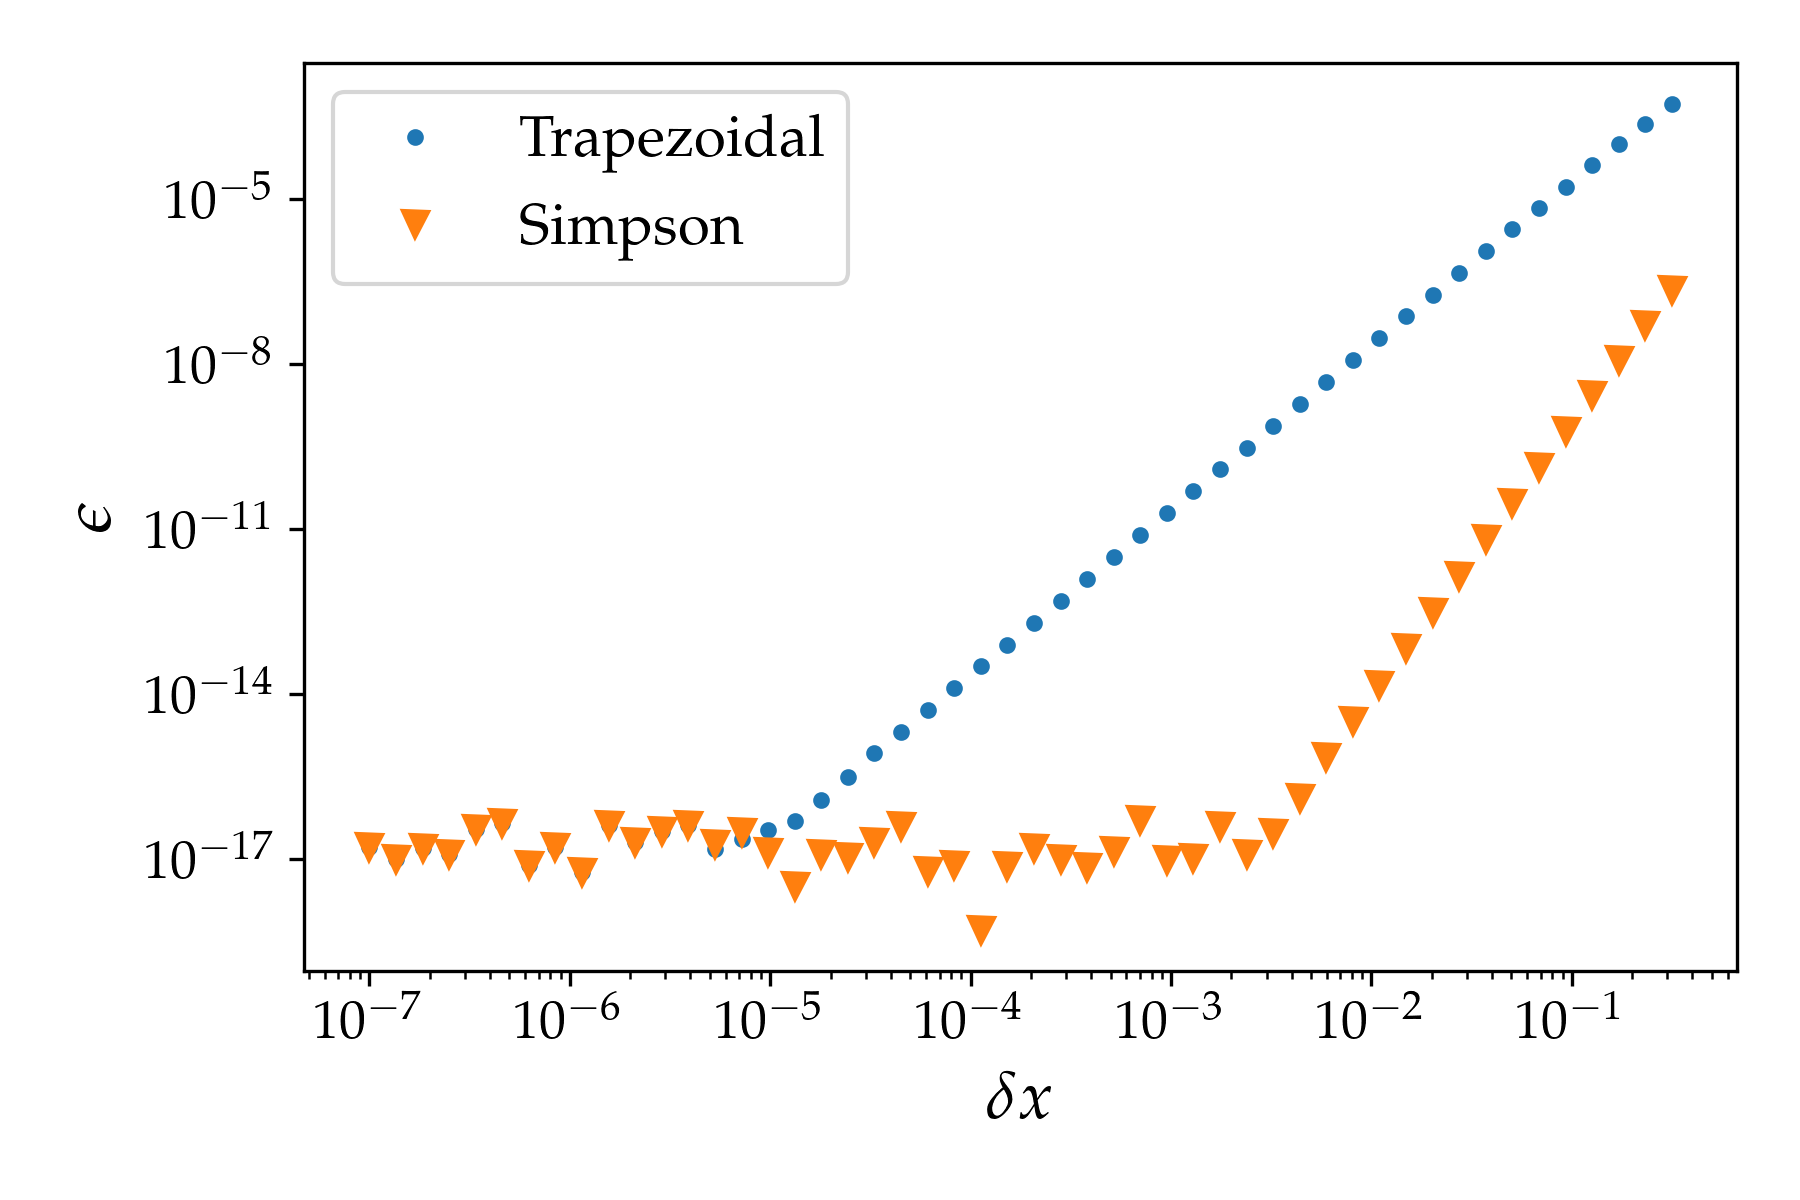
\includegraphics[width=0.8\linewidth]{images/20/confr_locals.png}
    \caption{Confronto tra gli algoritmi in forma locale, in funzione del passo $\delta x$.}
    \label{fig: confr_simp}
\end{figure}

\noindent I fit di seguito verificano i comportamenti che potevamo aspettarci dalla descrizione teorica che è stata fornita precedentemente, cioè dimostrano come la Regola dei trapezi \textit{locale} sia di ordine 3, mentre quella di Simpson di ordine 5.

\begin{figure}[H]
    \centering
    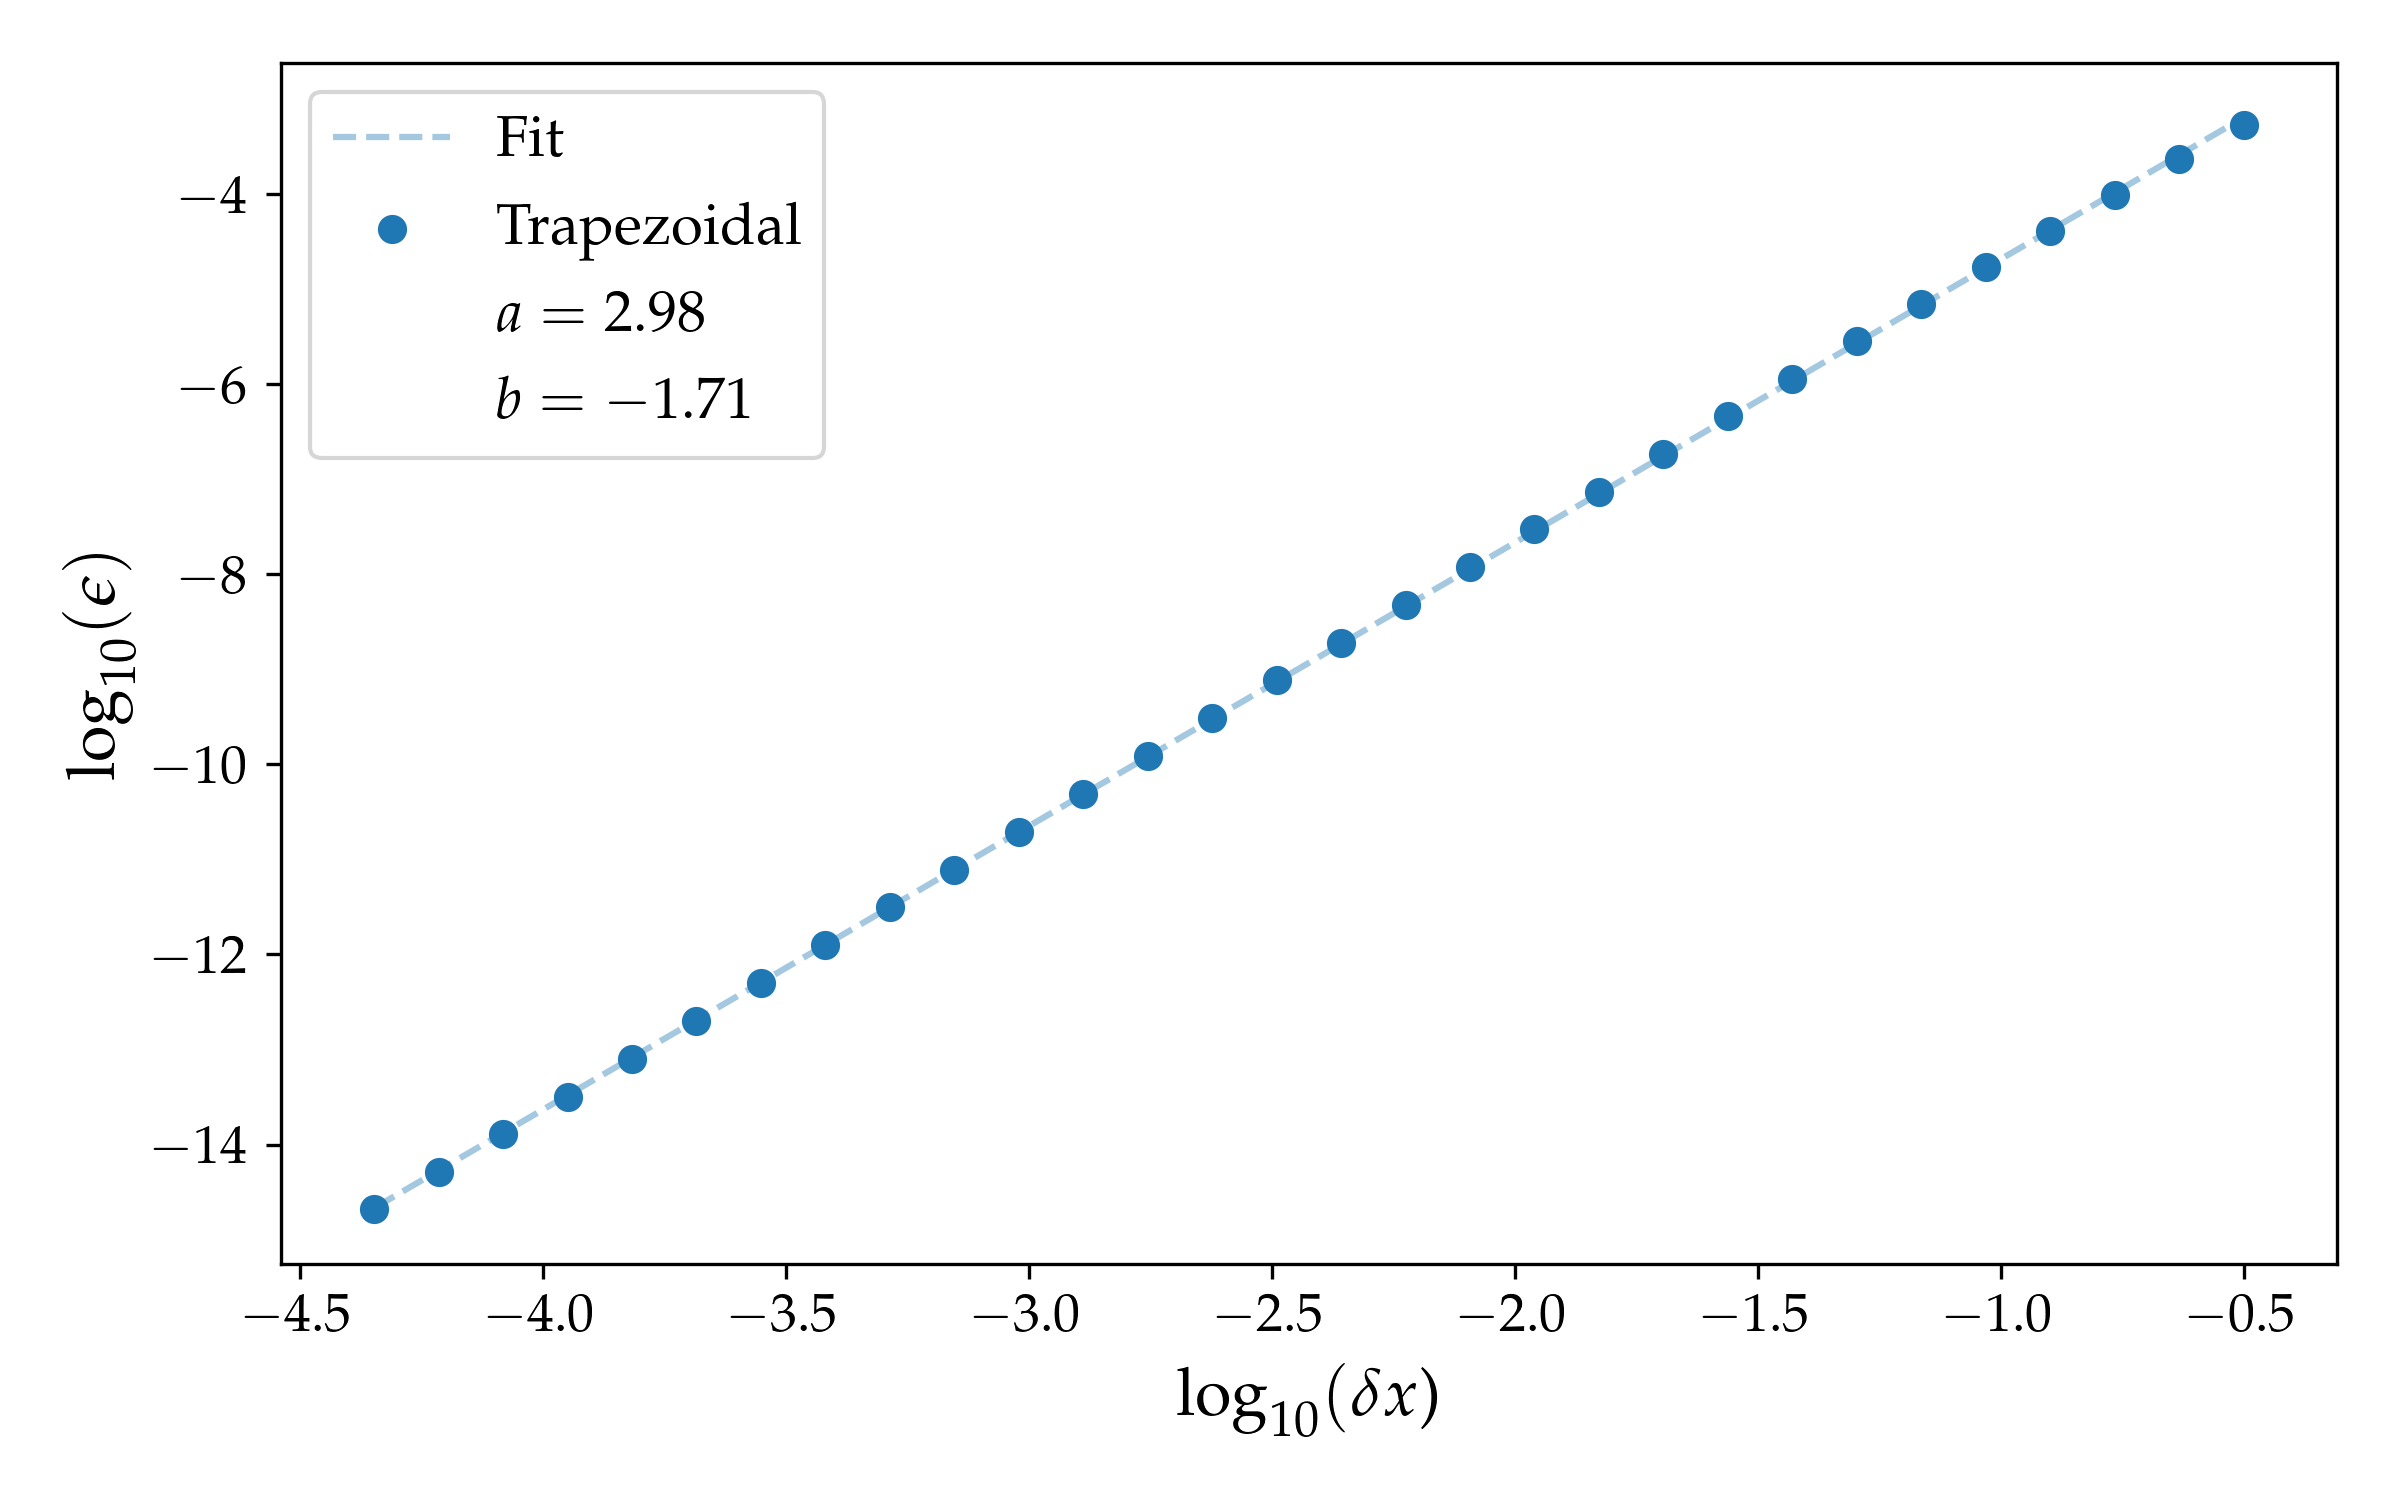
\includegraphics[width=0.8\linewidth]{images/20/Fit_LocTrap.png}
    \caption{Fit lineare (in forma logaritmica) del metodo dei trapezi in funzione dello step $\delta x$.}
    \label{fig: fit_locTrap}
\end{figure}

\begin{figure}[H]
    \centering
    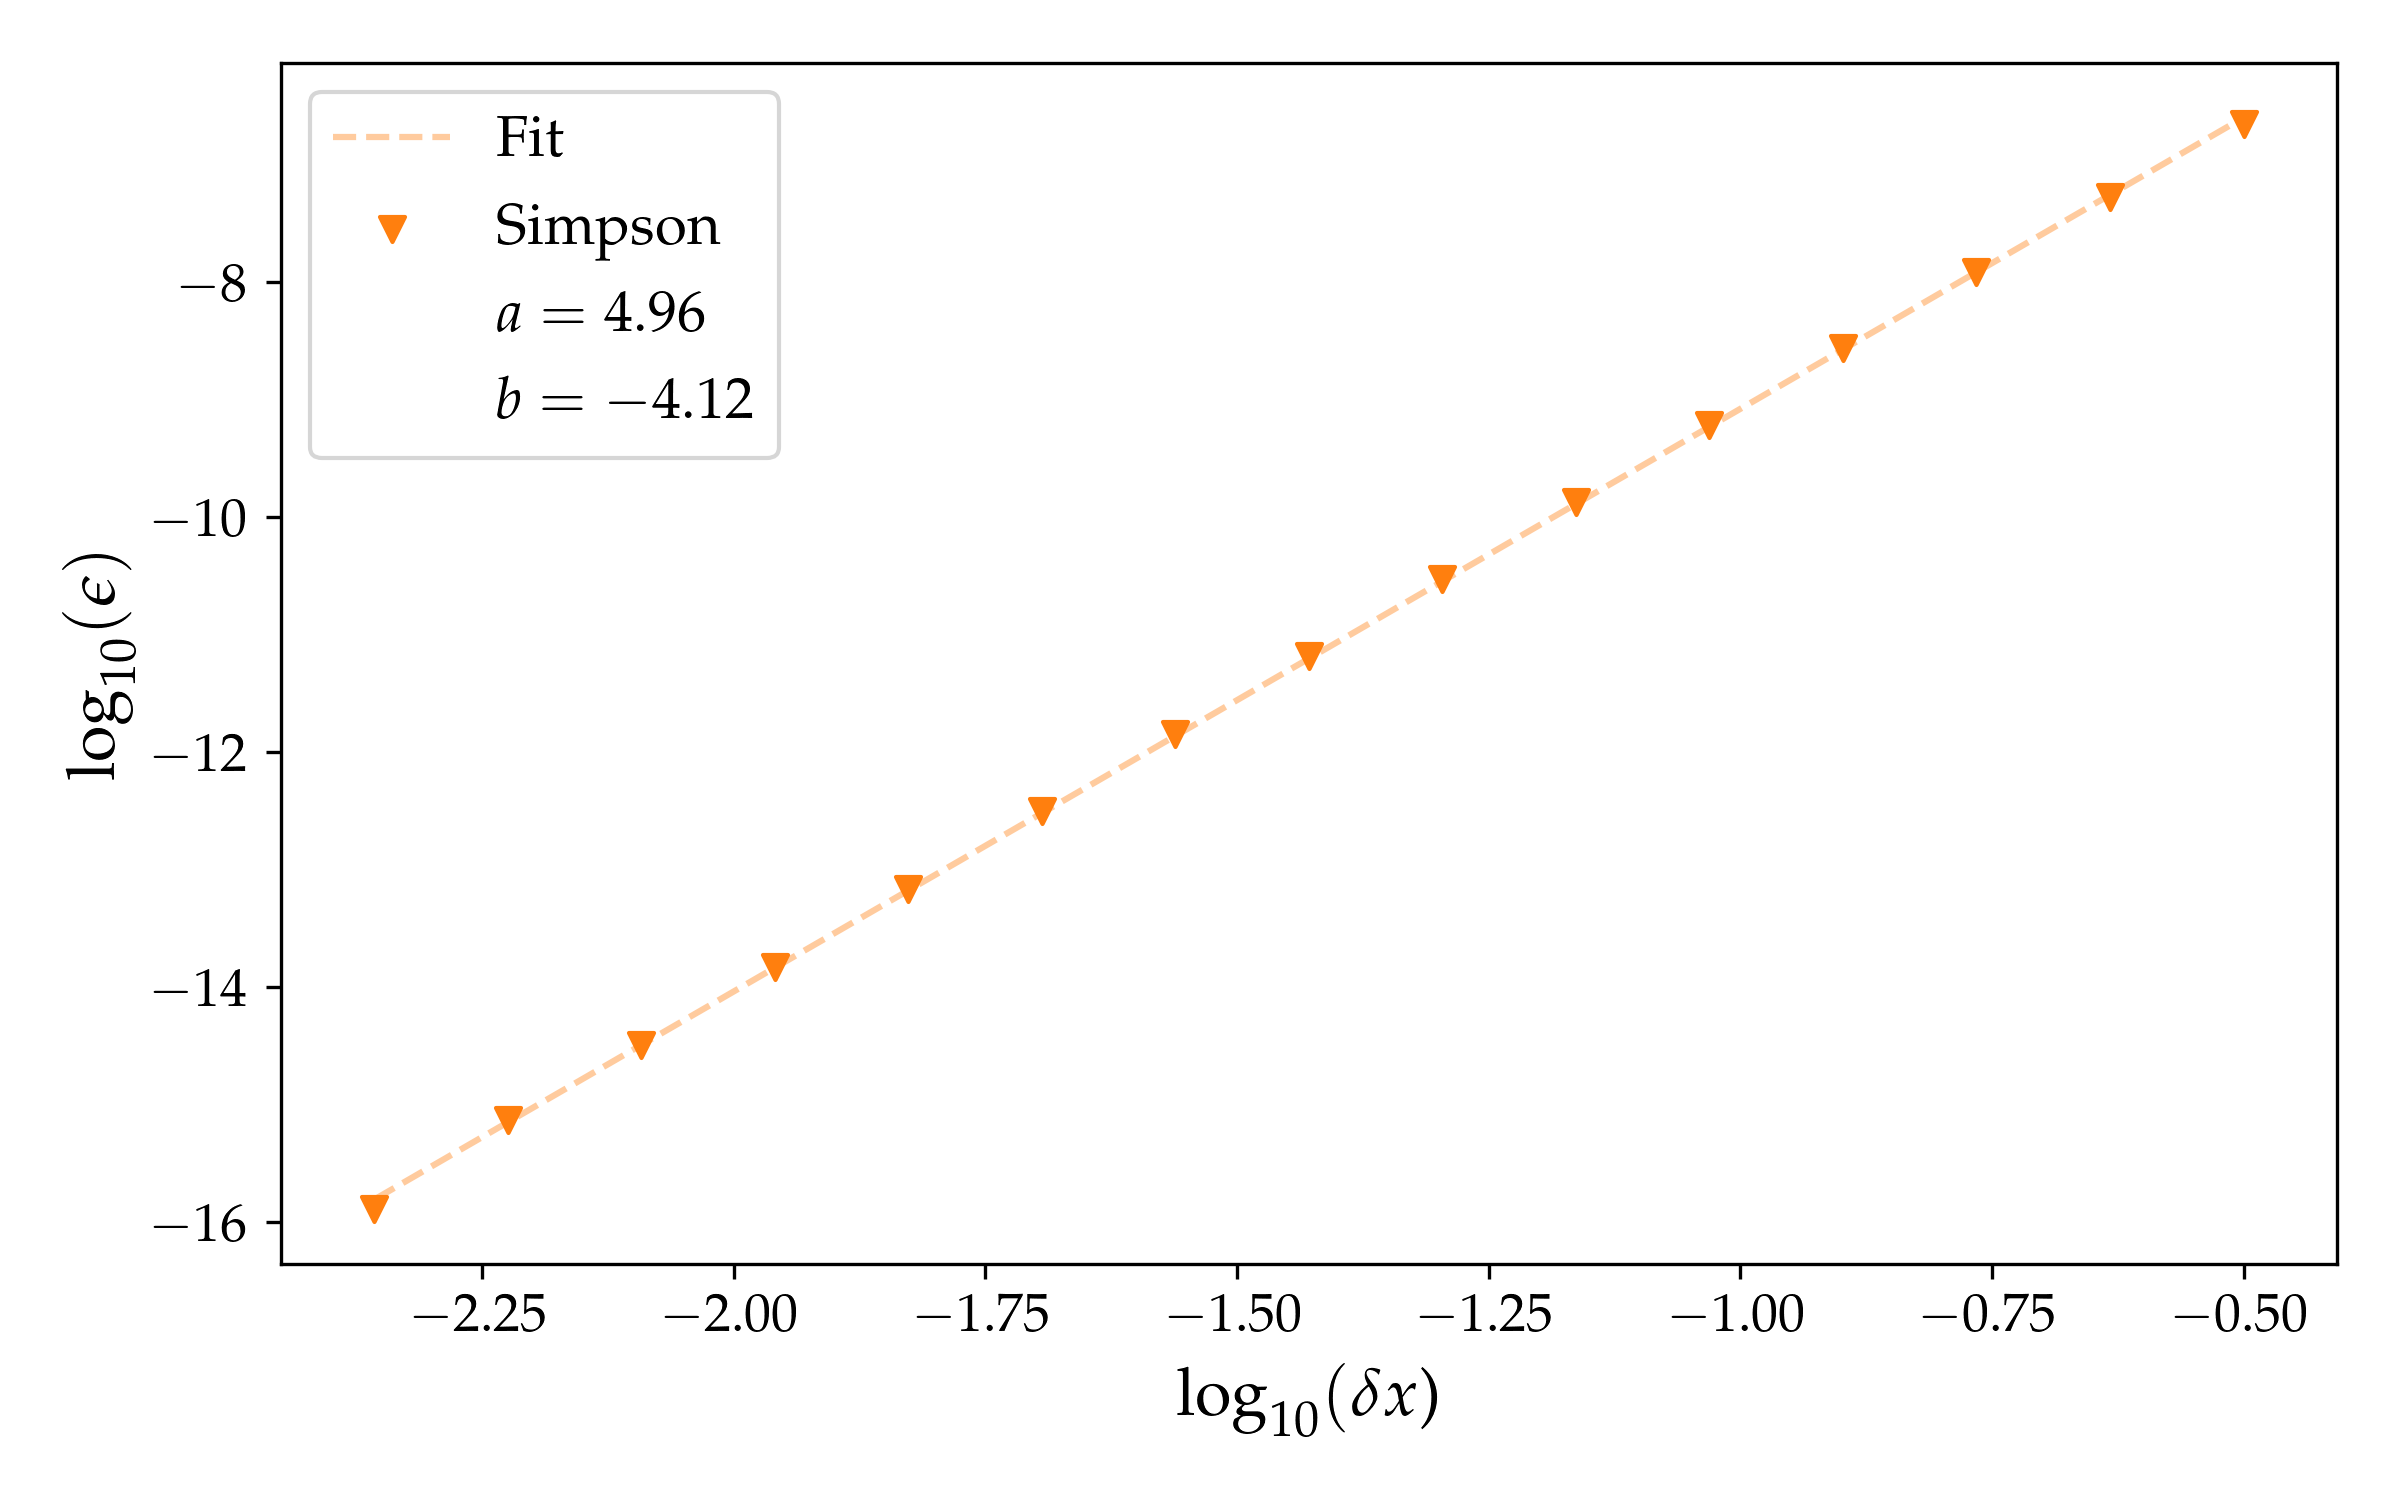
\includegraphics[width=0.8\linewidth]{images/20/Fit_LocSimp.png}
    \caption{Fit lineare (in forma logaritmica) del metodo di Simpson in funzione dello step $\delta x$.}
    \label{fig: fit_locSimp}
\end{figure}

\newpage











\section{Esercizio 8.1.2}
\subsection{Problem Statement}
Utilizzando le regole composite del trapezio e di Simpson, calcolare numericamente l'integrale adimensionale $I$ e verificare l'accuratezza e la convergenza attese del metodo. Per risolvere il problema del limite di integrazione che tende a infinito, considerare l'integrale troncato:

\begin{equation*}
I(x_{\text{max}}) = \int_{0}^{x_{\text{max}}} \frac{x^3}{e^x - 1} \, dx
\end{equation*}

\noindent e, prima di iniziare il calcolo, fornire una stima analitica di $x_{\text{max}}$ tale che l'errore di troncamento sia inferiore alla \textit{machine precision}. Una volta fissato $x_{\text{max}}$, studiare e confrontare lo scaling dei diversi metodi.


\subsection{Premessa Teorica}
In questo problema passiamo ad analizzare gli algoritmi globali dei trapezi e di Simpson, ricordando che entrambi perdono un ordine nello scaling, diventando uno del secondo ordine, l'altro del quarto.

\subsection{Metodi Numerici e Algoritmi}
L'esercizio richiede di risolvere
\begin{equation*}
I = \int_{0}^{+\infty} \frac{x^3}{e^x - 1} \, dx\ \left ( = \frac{\pi^4}{15} \approx 6.49 \right)
\end{equation*}
che è però impossibile, lavorando dal punto di vista numerico: dobbiamo riuscire a isolare su un intervallo finito il nostro campo di azione, cioè escludendo quella coda dell'integrale, per\\ $x_{max} \in (0, +\infty)$:
$$\bar I(x_{\text{max}}) = \int_{x_{\text{max}}}^{\infty} \frac{x^3}{e^x - 1} \, dx \le \varepsilon $$  

\bigskip\noindent
Ho valutato analiticamente $x_{max}$ accettando l'approssimazione che $x_{max}\gg1$: in questo modo
\begin{align*}
e^x -1 &\approx e^x \\
\bar I &\approx \int_{x_{max}}^\infty e^{-x}x^3\ dx > 0\ , \quad x_{max}>0
\end{align*}
cioè la $\Gamma(4, x_{max})$. Risolvo per \textit{IBP} e ottengo:
\[
    \bar I = e^{-x_{max}}(x_{max}^3 + 3x_{max}^2 + 6x_{max} + 6) \le \varepsilon \\
\]
riordinando i termini e semplificando la scrittura:
\begin{align*}
    0 < \bar I / \varepsilon &\le 1 \\
    \log(\bar I/ \varepsilon) &\le 0\\
    \log(\bar I) - \log(\varepsilon) &\le 0
\end{align*}
ridenfinendo infine come
\begin{align*}
    h_{zero}(x) &= \log(\bar I) - \log(\varepsilon)\\
     &=\log(x^3 + 3x^2 + 6x + 6) -  (x + \log(\varepsilon))\\
\end{align*}

\noindent Un algoritmo di ricerca degli zeri, come quelli che abbiamo sviluppato in precedenza, risulta perfetto per la stima necessaria, scegliamo bisezione. Dopo aver studiato $h_{zero}(x)$ in Fig. \ref{fig: zero_res_int}, e avendo scelto un intervallo in cui inizializzare l'algoritmo, troviamo la radice dell'equazione (guardiamo l'uguaglianza e ci ricordiamo della disequazione più avanti).

\noindent La ricerca di $h_{zero}(x) = 0$ restituisce il valore $x_{max} = 48.551645373827725$.

\begin{figure}[H]
    \centering
    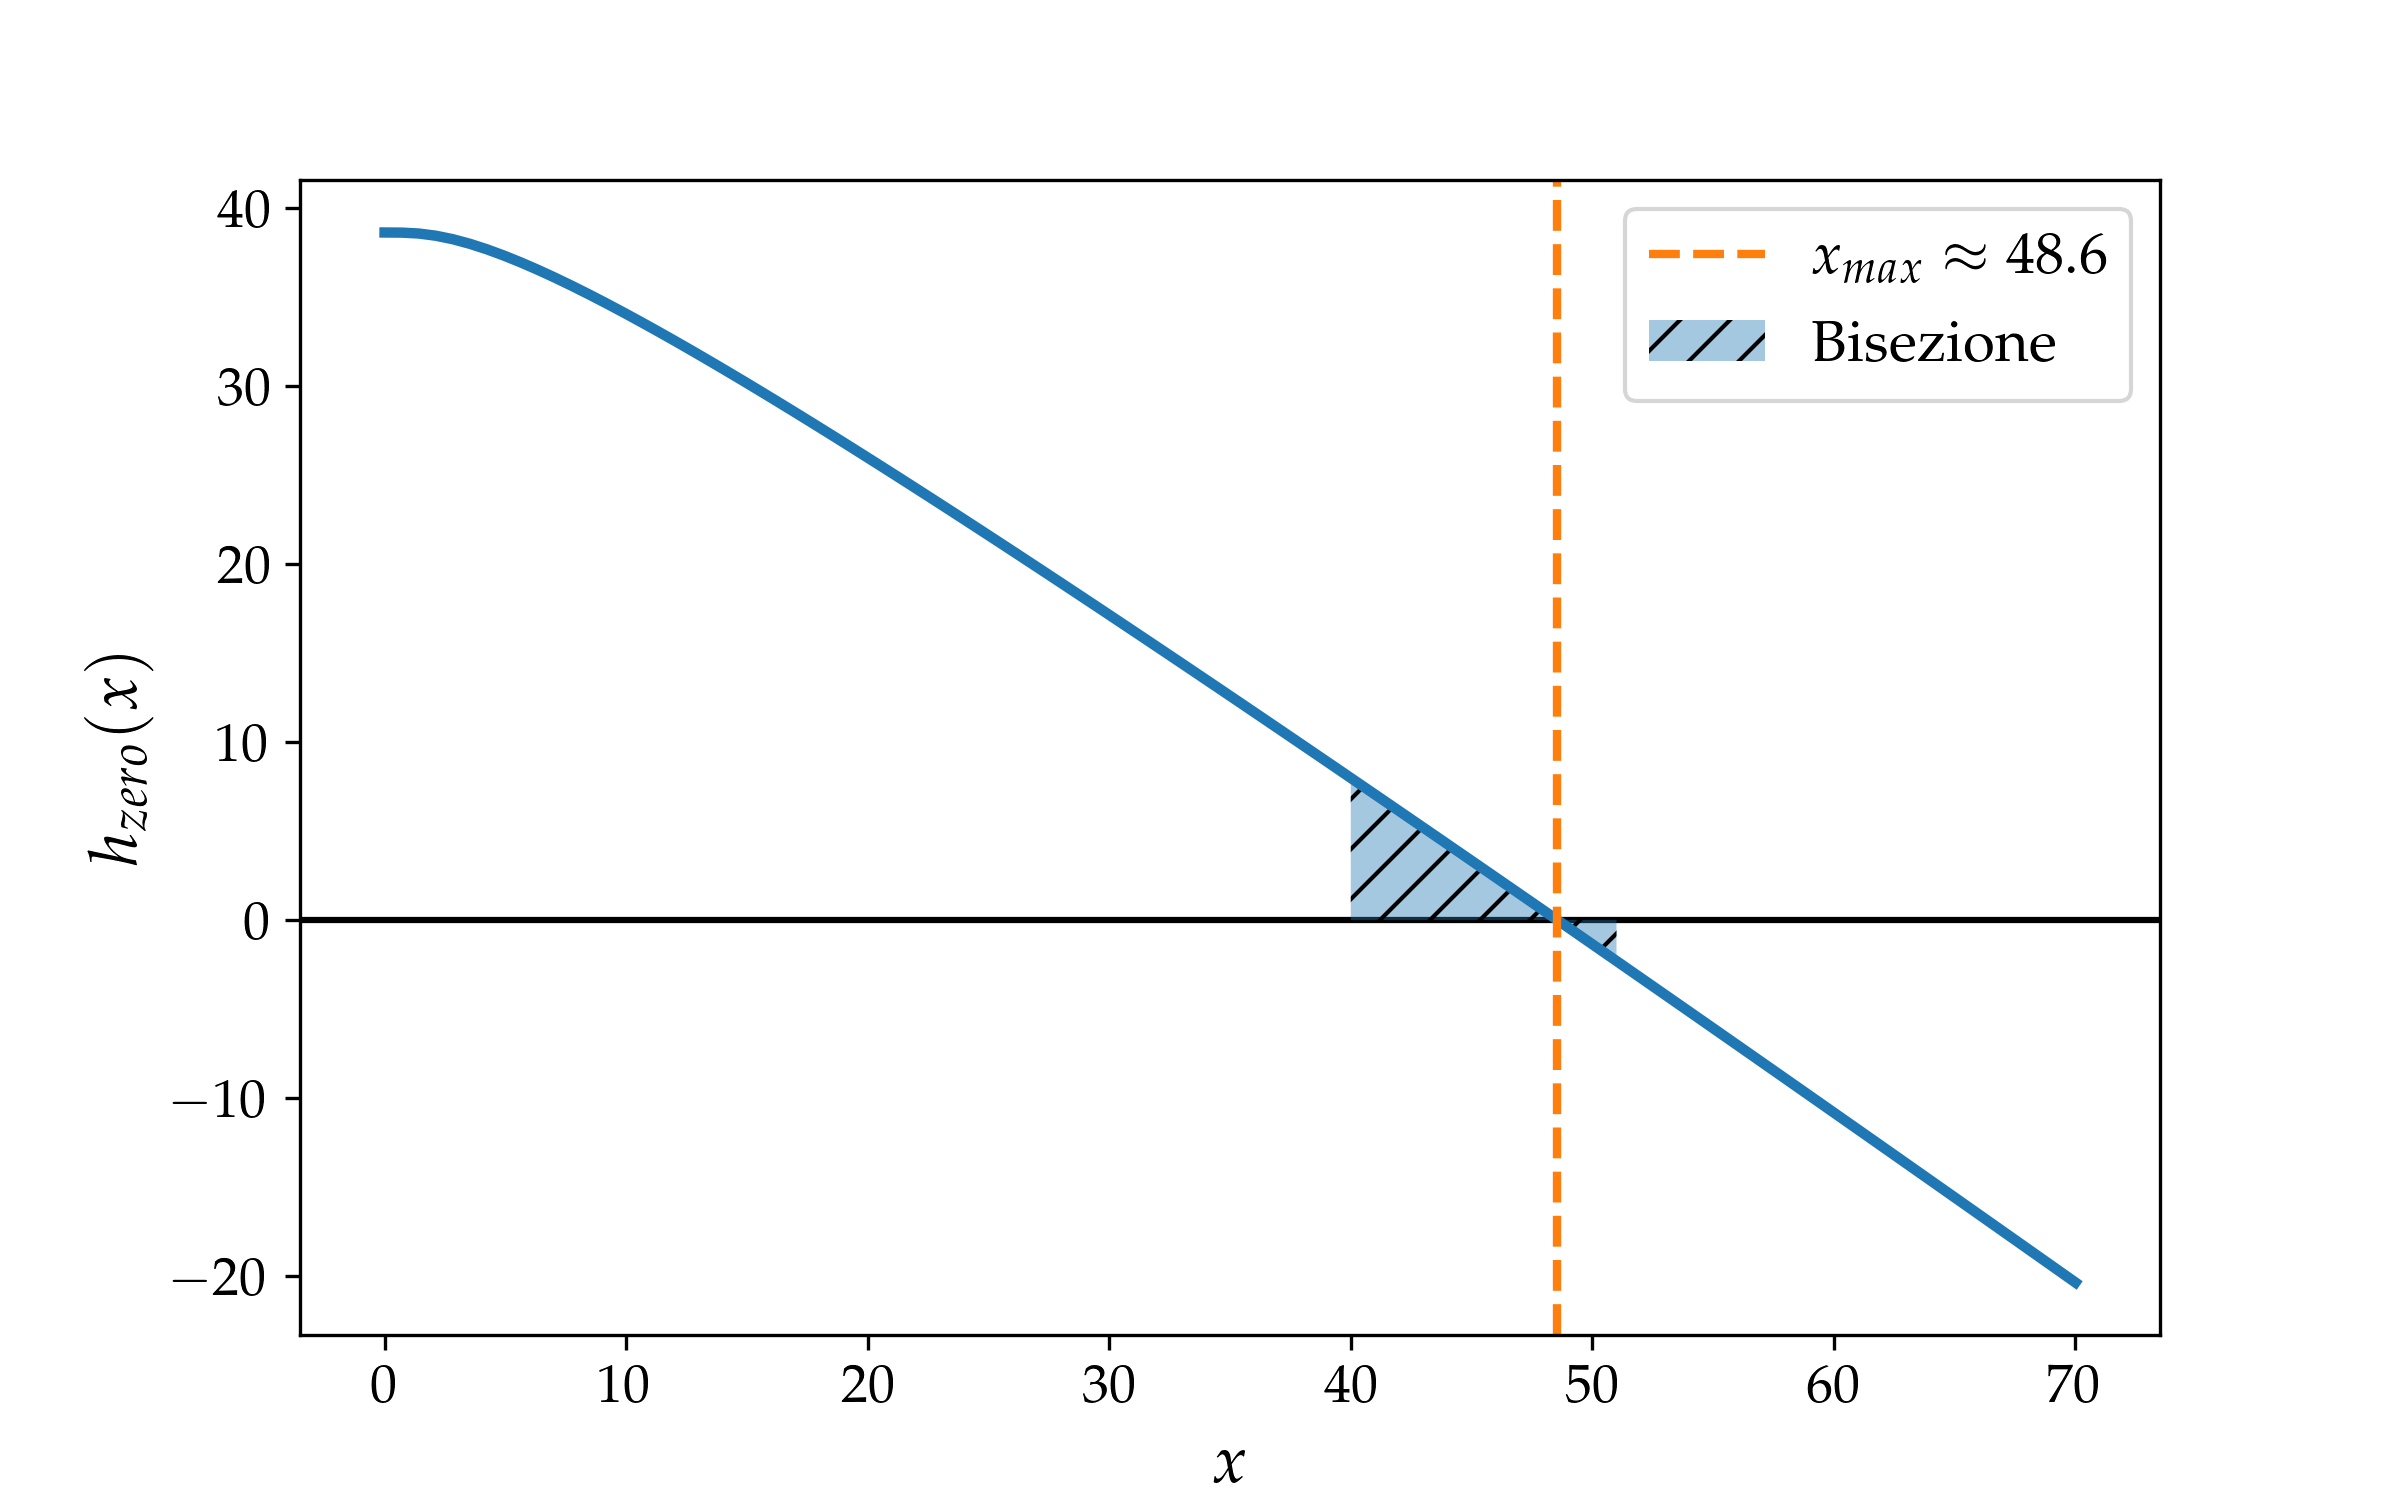
\includegraphics[width=0.8\linewidth]{images/20/zero_res.png}
    \caption{Ricerca degli zeri sulla funzione $g_{zero}(x)$ con l'algoritmo di Bisezione: è stato scelto l'intervallo $x\in [20, 50]$.}
    \label{fig: zero_res_int}
\end{figure}

\noindent La condizione approssimata è che si ottiene è quindi che $x_{max} > 49$. In Fig. \ref{fig: x_int_conf} la verifica del nostro calcolo, valutando l'andamento della funzione integrale:
\[
F(x) = \int_0^x f(t)\ dt
\]
Infine segue un ultimo confronto riepilogativo, per il confronto anche con il metodo dei trapezi e per valutare brevemente l'approssimazione necessaria che facciamo per $x=0 \to x =10^{-9}$.

\begin{elegantcode}
a = 1e-09
b = 48.551645373827725

True = 6.493939402266828
residual = 3.333333333333334e-28


Trapezi:

I_t = 6.4939394022668235
leftover = 1.0000000734565665e-16
diff = 4.440892098500626e-15


Simpson:

I_s = 6.493939402266805
leftover = 9.996869800764608e-17
diff = 2.3092638912203256e-14
\end{elegantcode}


\begin{figure}[H]
    \centering
    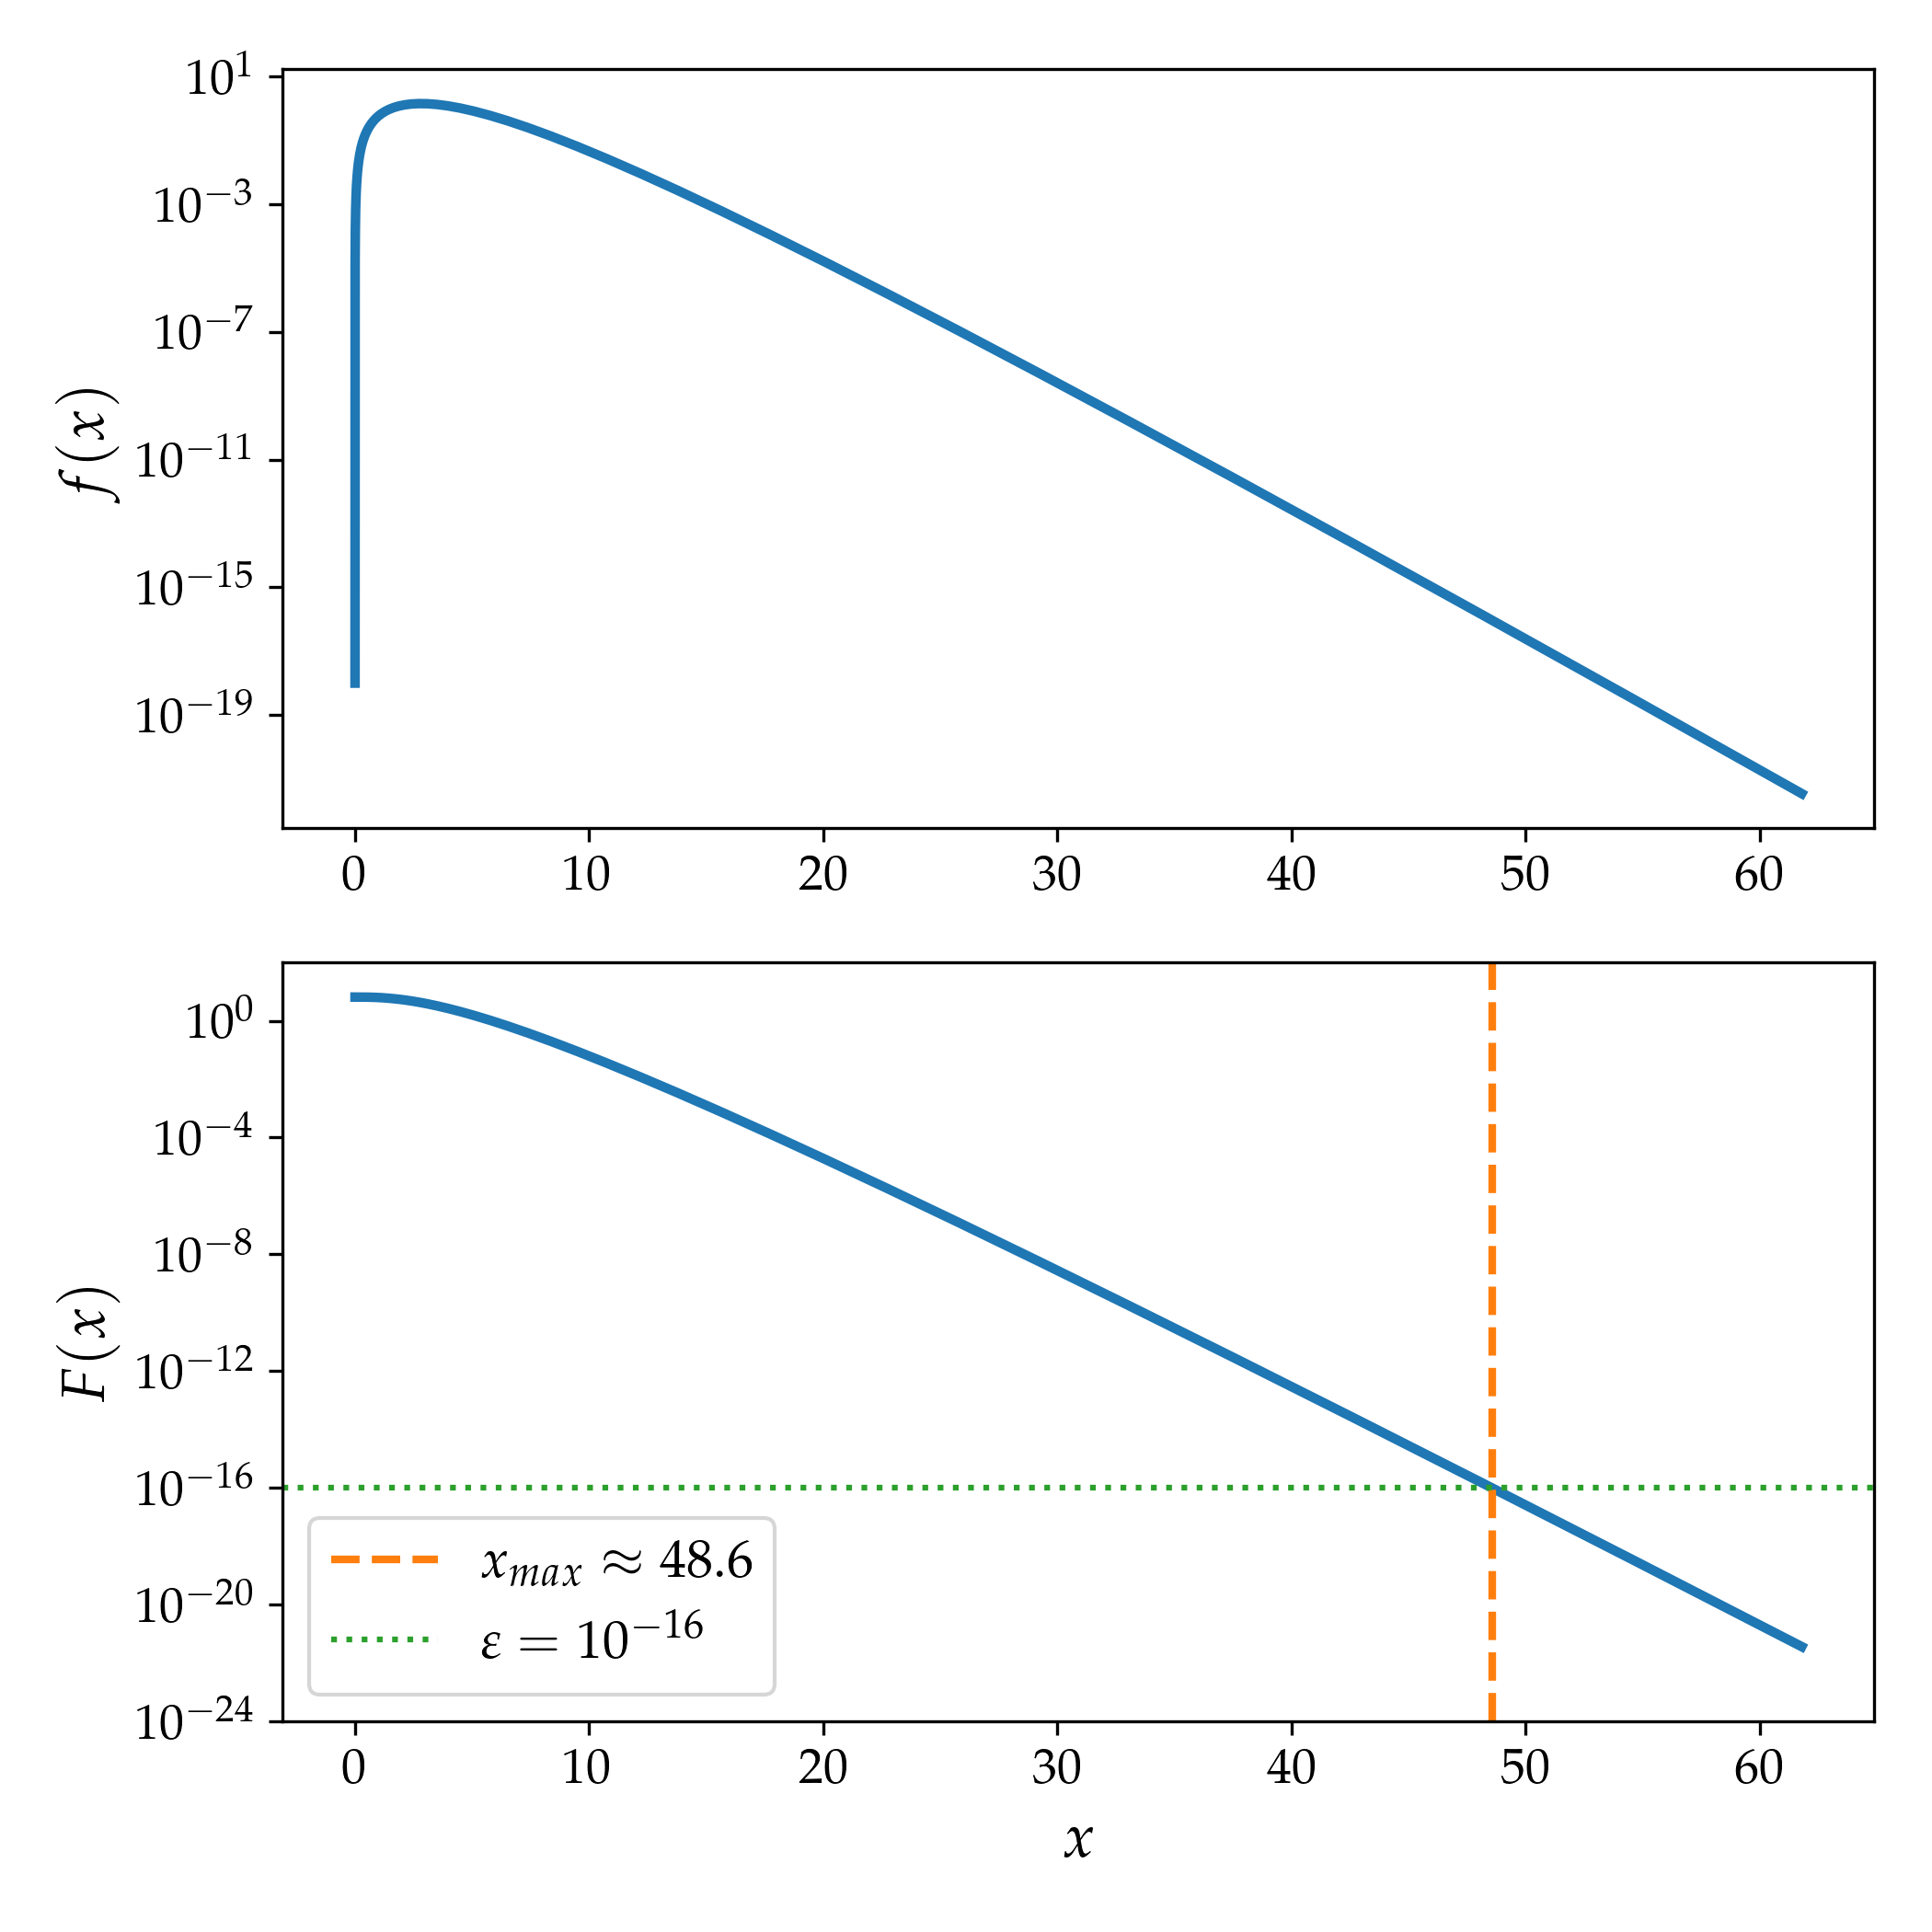
\includegraphics[width=0.7\linewidth]{images/20/x_int_conf.png}
    \caption{Andamento delle funzioni $f(x),F(x)$. La \textit{treshold} fissata a $\varepsilon=10^{-16}$ è coerente con il valore che abbiamo appena determinato.}
    \label{fig: x_int_conf}
\end{figure}


\subsection{Risultati e Discussione}

Si mostrano di seguito i risultati del confronto dei due metodi, Fig. \ref{fig: glob_conf}, e dei fit sui singoli, Fig. \ref{fig: fit_trap_glob} e \ref{fig: fit_simp_glob}. Per i fit si seleziona solo la parte più a destra del confronto, escludendo le sezioni in cui si forma il plateau relativo alla \textit{machine precision}.

\noindent È lampante osservare dal primo grafico, ma dai fit abbiamo la conferma rigorosa, che se il metodo di Simpson si comporta come ci attendevamo di rilevare, non fa lo stesso quello dei trapezi, che produce un andamento a convergenza del quarto ordine. Questo commento non contraddice ciò che abbiamo precedentemente affermato, però mette in luce un fenomeno numerico che deve star avvenendo per aumentare l'ordine di convergenza nel metodo.

\medskip\noindent
L'andamento numerico osservato suggerisce una superconvergenza del metodo dei trapezi per questa specifica funzione.\\
Il metodo dei trapezi ha errore locale 

\begin{equation*}
    \epsilon_{L, i} = -\frac{1}{12} \delta x^3 f''(x_i) -\frac{1}{24} \delta x^4 f'''(x_i) + O(\delta x^5) \,.
\end{equation*}
passando all'errore totale (cioè relativo al metodo in forma composta), che è l'accumulazione degli errori locali:

$$\epsilon_G = \sum \epsilon_{L,i} = -\frac{1}{12}\delta x^2 \sum f''(x_i)\delta x - \frac{1}{24}\delta x^3 \sum f'''(x_i)\delta x + O(\delta x^4)$$

sviluppando ulteriormente fino al quarto ordine e ricordando:

$$\sum g(x_i)\delta x = \int_a^b g(x)dx - \frac{\delta x}{2} (g(b) - g(a)) + O(\delta x^2)$$

Applicandolo alle nostre derivate:

\begin{align*}
    \sum f''(x_i)\delta x &= \int_a^b f''(x)dx - \frac{\delta x}{2} \left( f'' (b)-f'' (a) \right)  + O(\delta x^2)  \\
    &= (f'(b) - f'(a)) - \frac{\delta x}{2} \left( f'' (b)-f'' (a) \right)  + O(\delta x^2)\\
    \sum f'''(x_i) \delta x &= \int_a^b f'''(x)dx = f''(b) - f''(a) + O(\delta x)
\end{align*}

\begin{align*}
    \epsilon_G =& -\frac{1}{12}\delta x^2 (f'(b) - f'(a)) + \frac{1}{24}\delta x^3 (f''(b) - f''(a)) - \frac{1}{24}\delta x^3 (f''(b) - f''(a)) + O(\delta x^4)\\
    =& -\frac{1}{12}\delta x^2 (f'(b) - f'(a))   + O(\delta x^4)
\end{align*}

\noindent sapendo che per la funzione specifica con cui stiamo lavorando vale che la derivata prima è nulla in entrambi gli estremi $a, b$ (Fig. \ref{fig: der_conf}), concludiamo che $\epsilon = O(\delta x^4)$.

\noindent L'algoritmo è quindi dell'ordine 4. Questo tipo di fenomeno viene definito superconvergenza e rappresenta l'occasione di ricorrere ad algoritmi in generale meno performativi, ma ottimi per alcune loro caratteristiche per problemi specifici.

\begin{figure}[H]
    \centering
    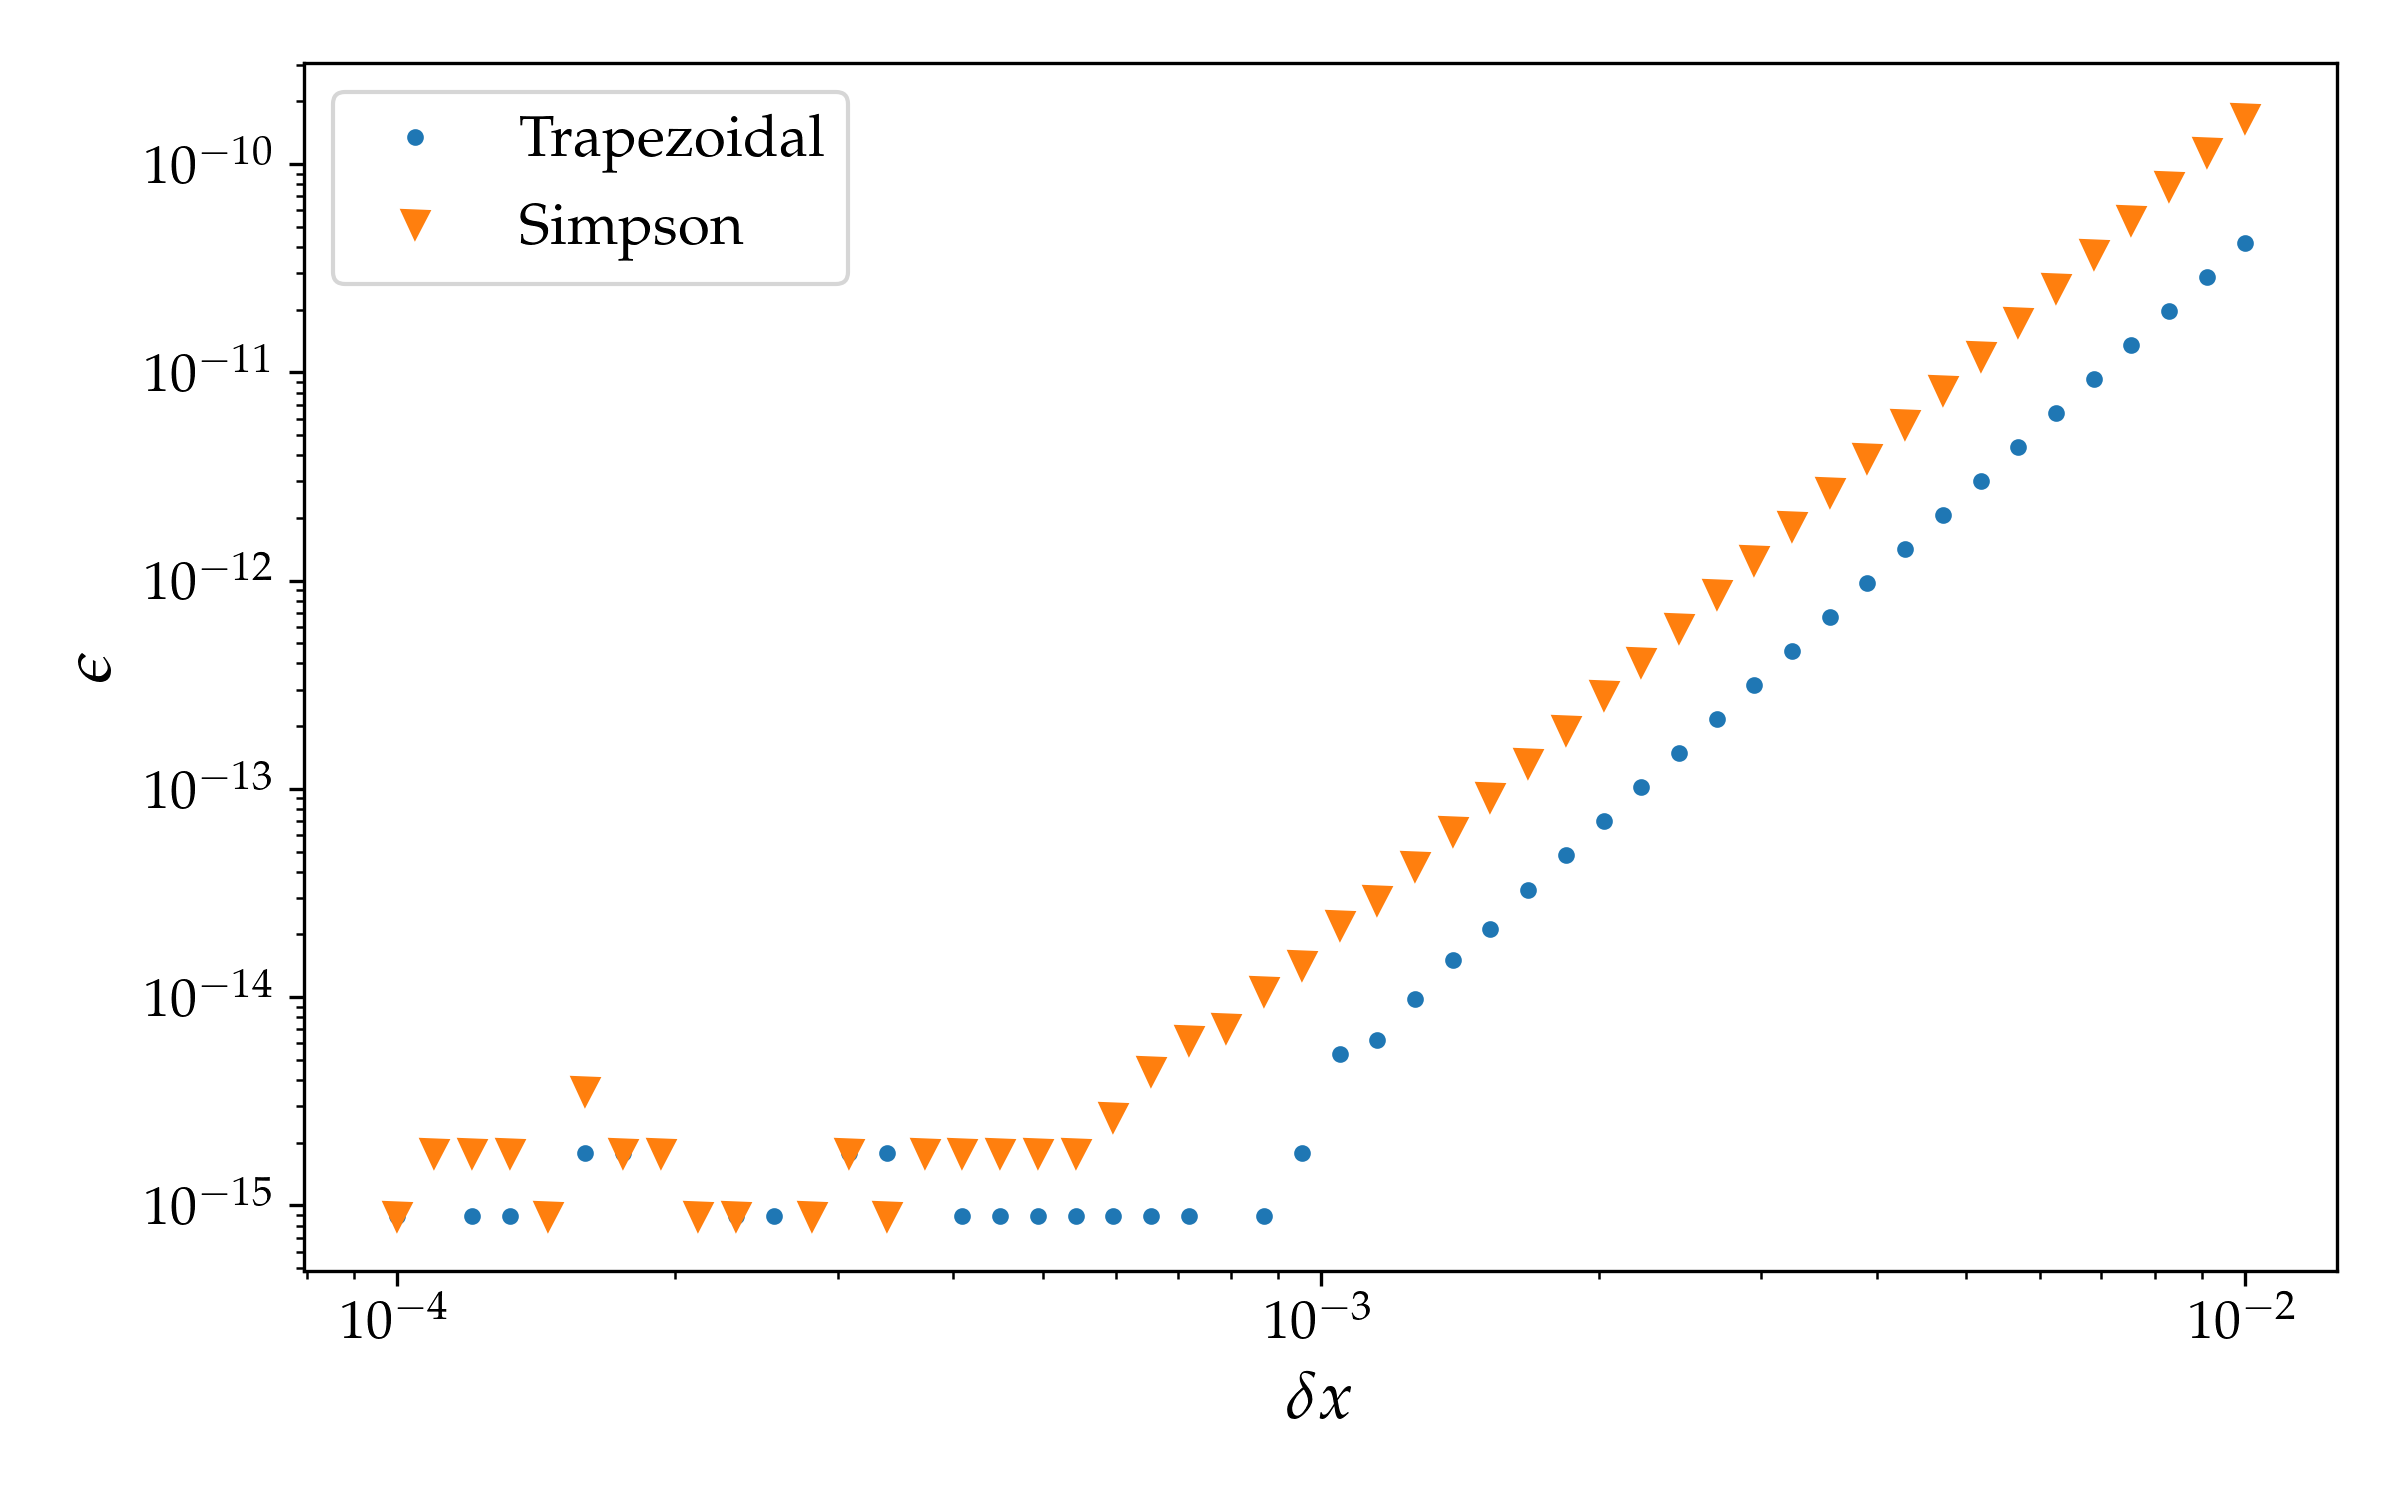
\includegraphics[width=0.8\linewidth]{images/20/confr_glob.png}
    \caption{Confronto fra gli andamenti dei due metodi per integrazione numerica. Entrambi raggiungono il plateau di \textit{machine precision} da cui non è più possibile osservare l'ordine di convergenza.}
    \label{fig: glob_conf}
\end{figure}

\begin{figure}[H]
    \centering
    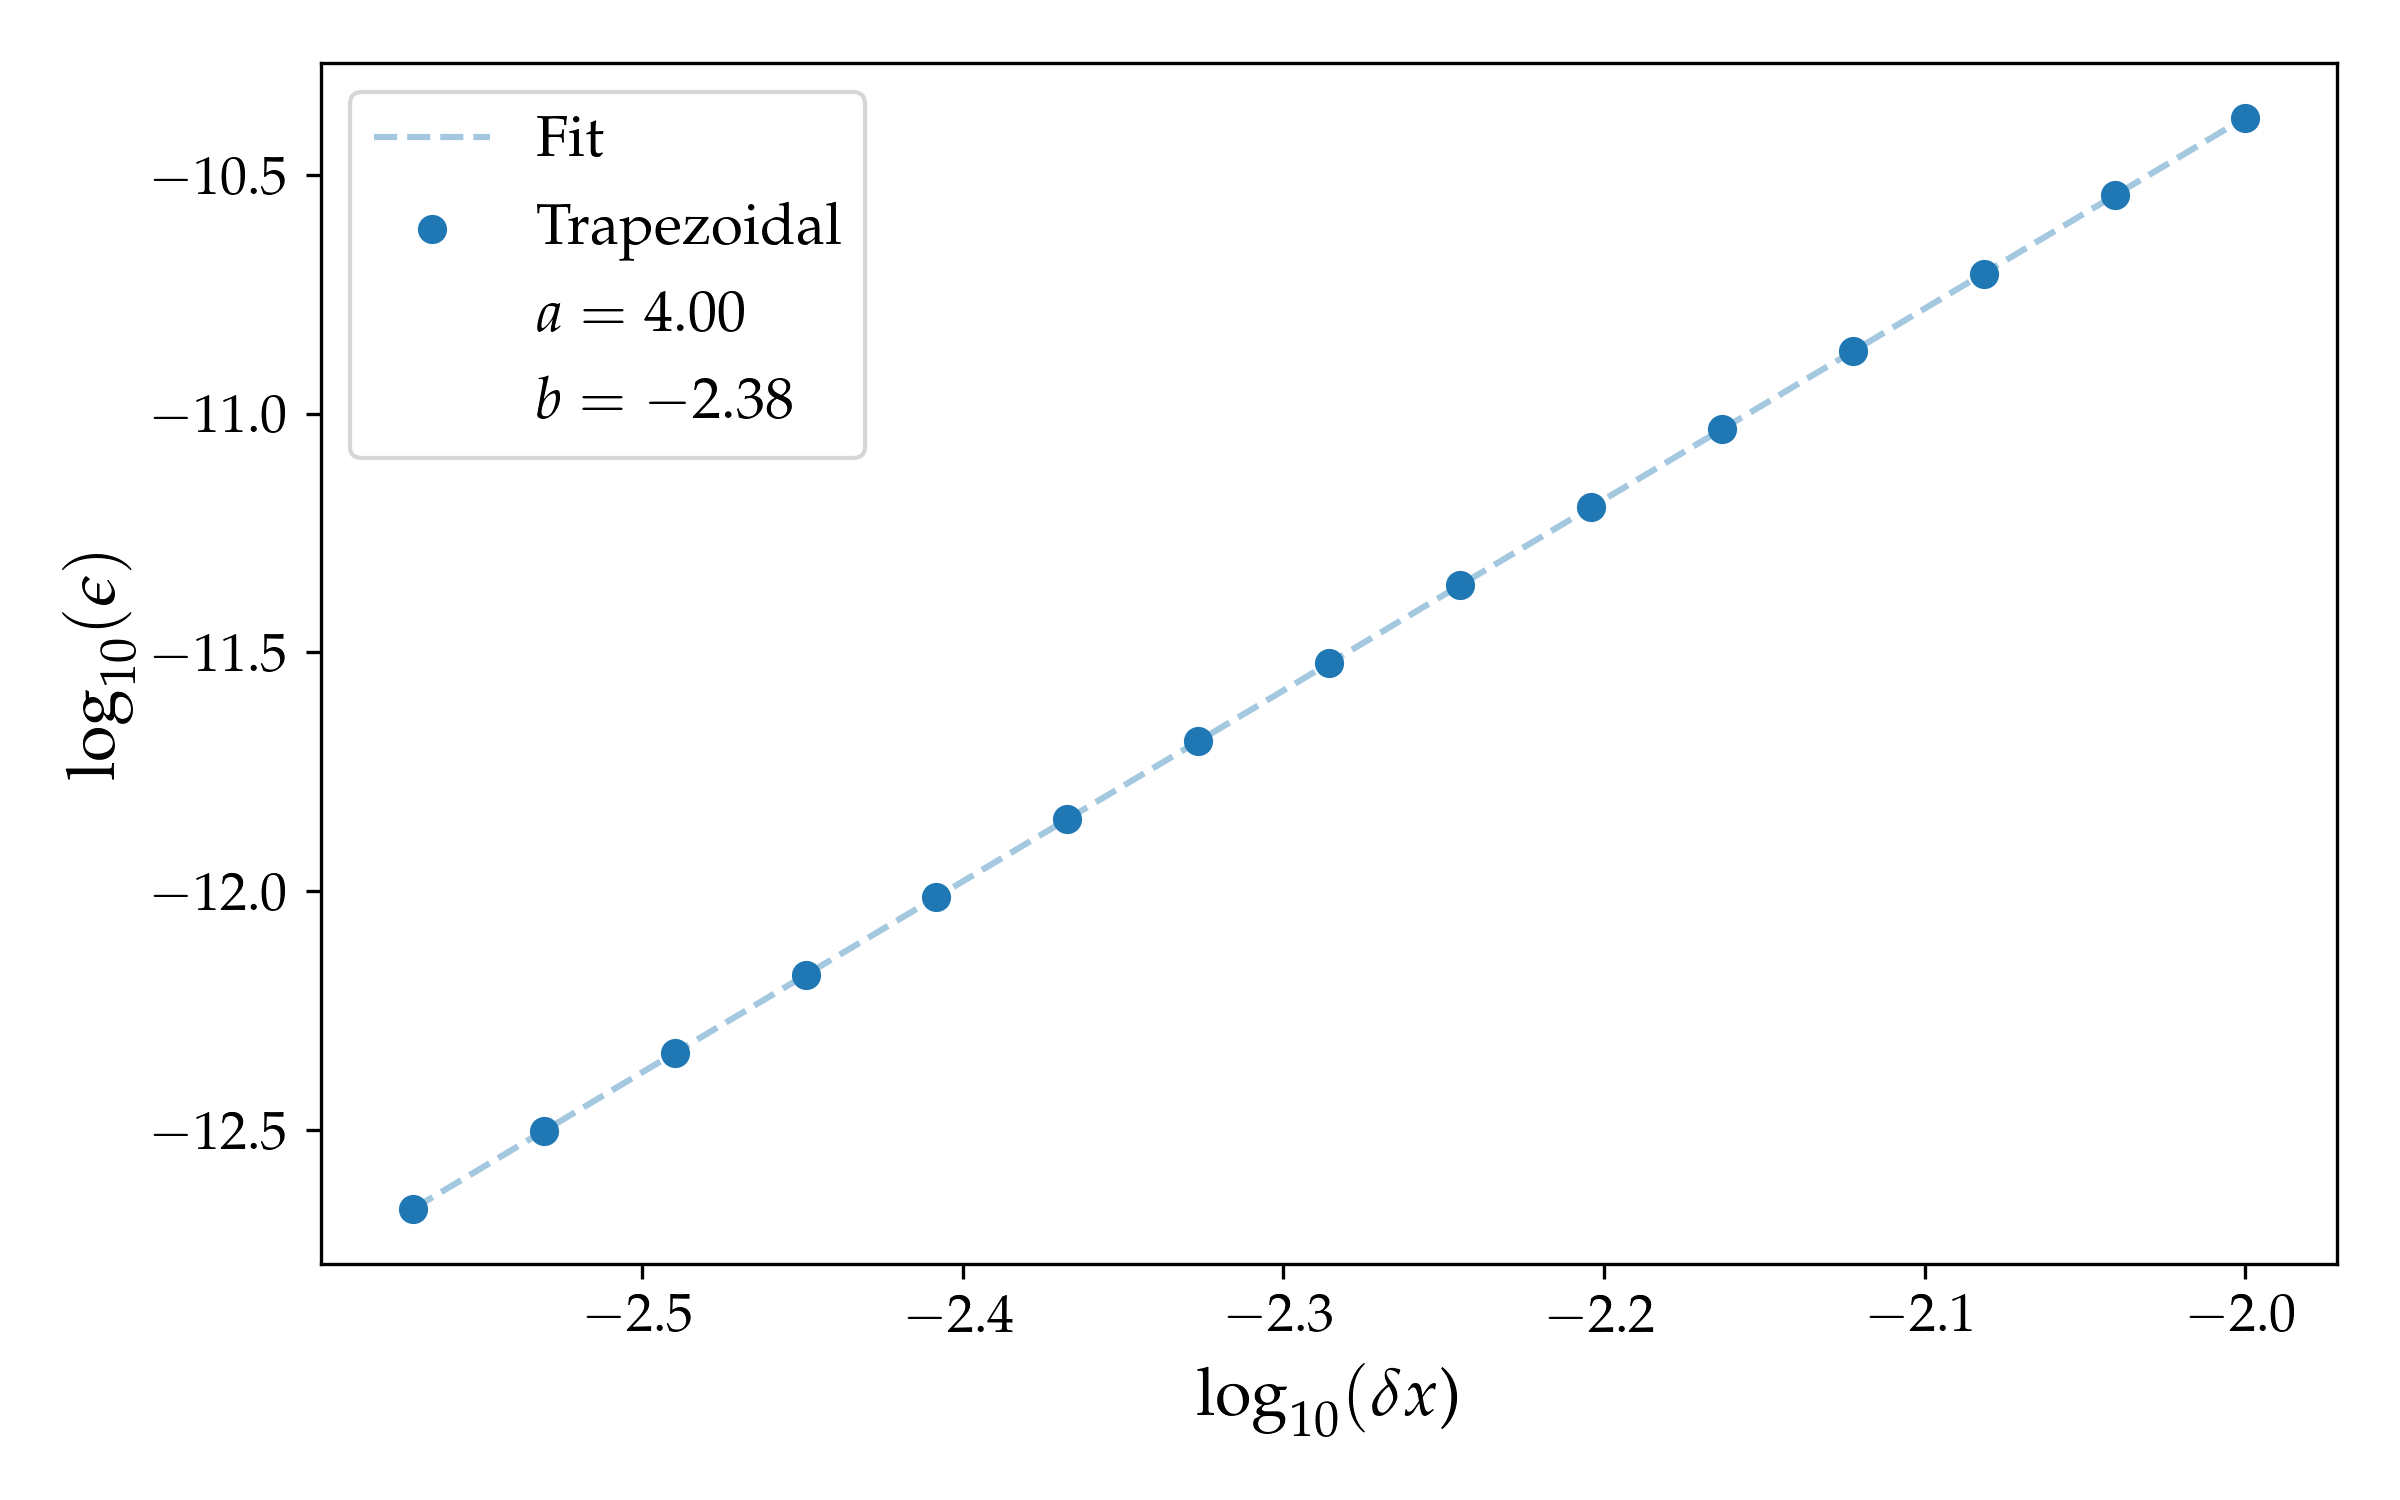
\includegraphics[width=0.8\linewidth]{images/20/Fit_gl_trap.png}
    \caption{Fit sulla Regola dei trapezi composta in funzione del passo $\delta x$.}
    \label{fig: fit_trap_glob}
\end{figure}

\begin{figure}[H]
    \centering
    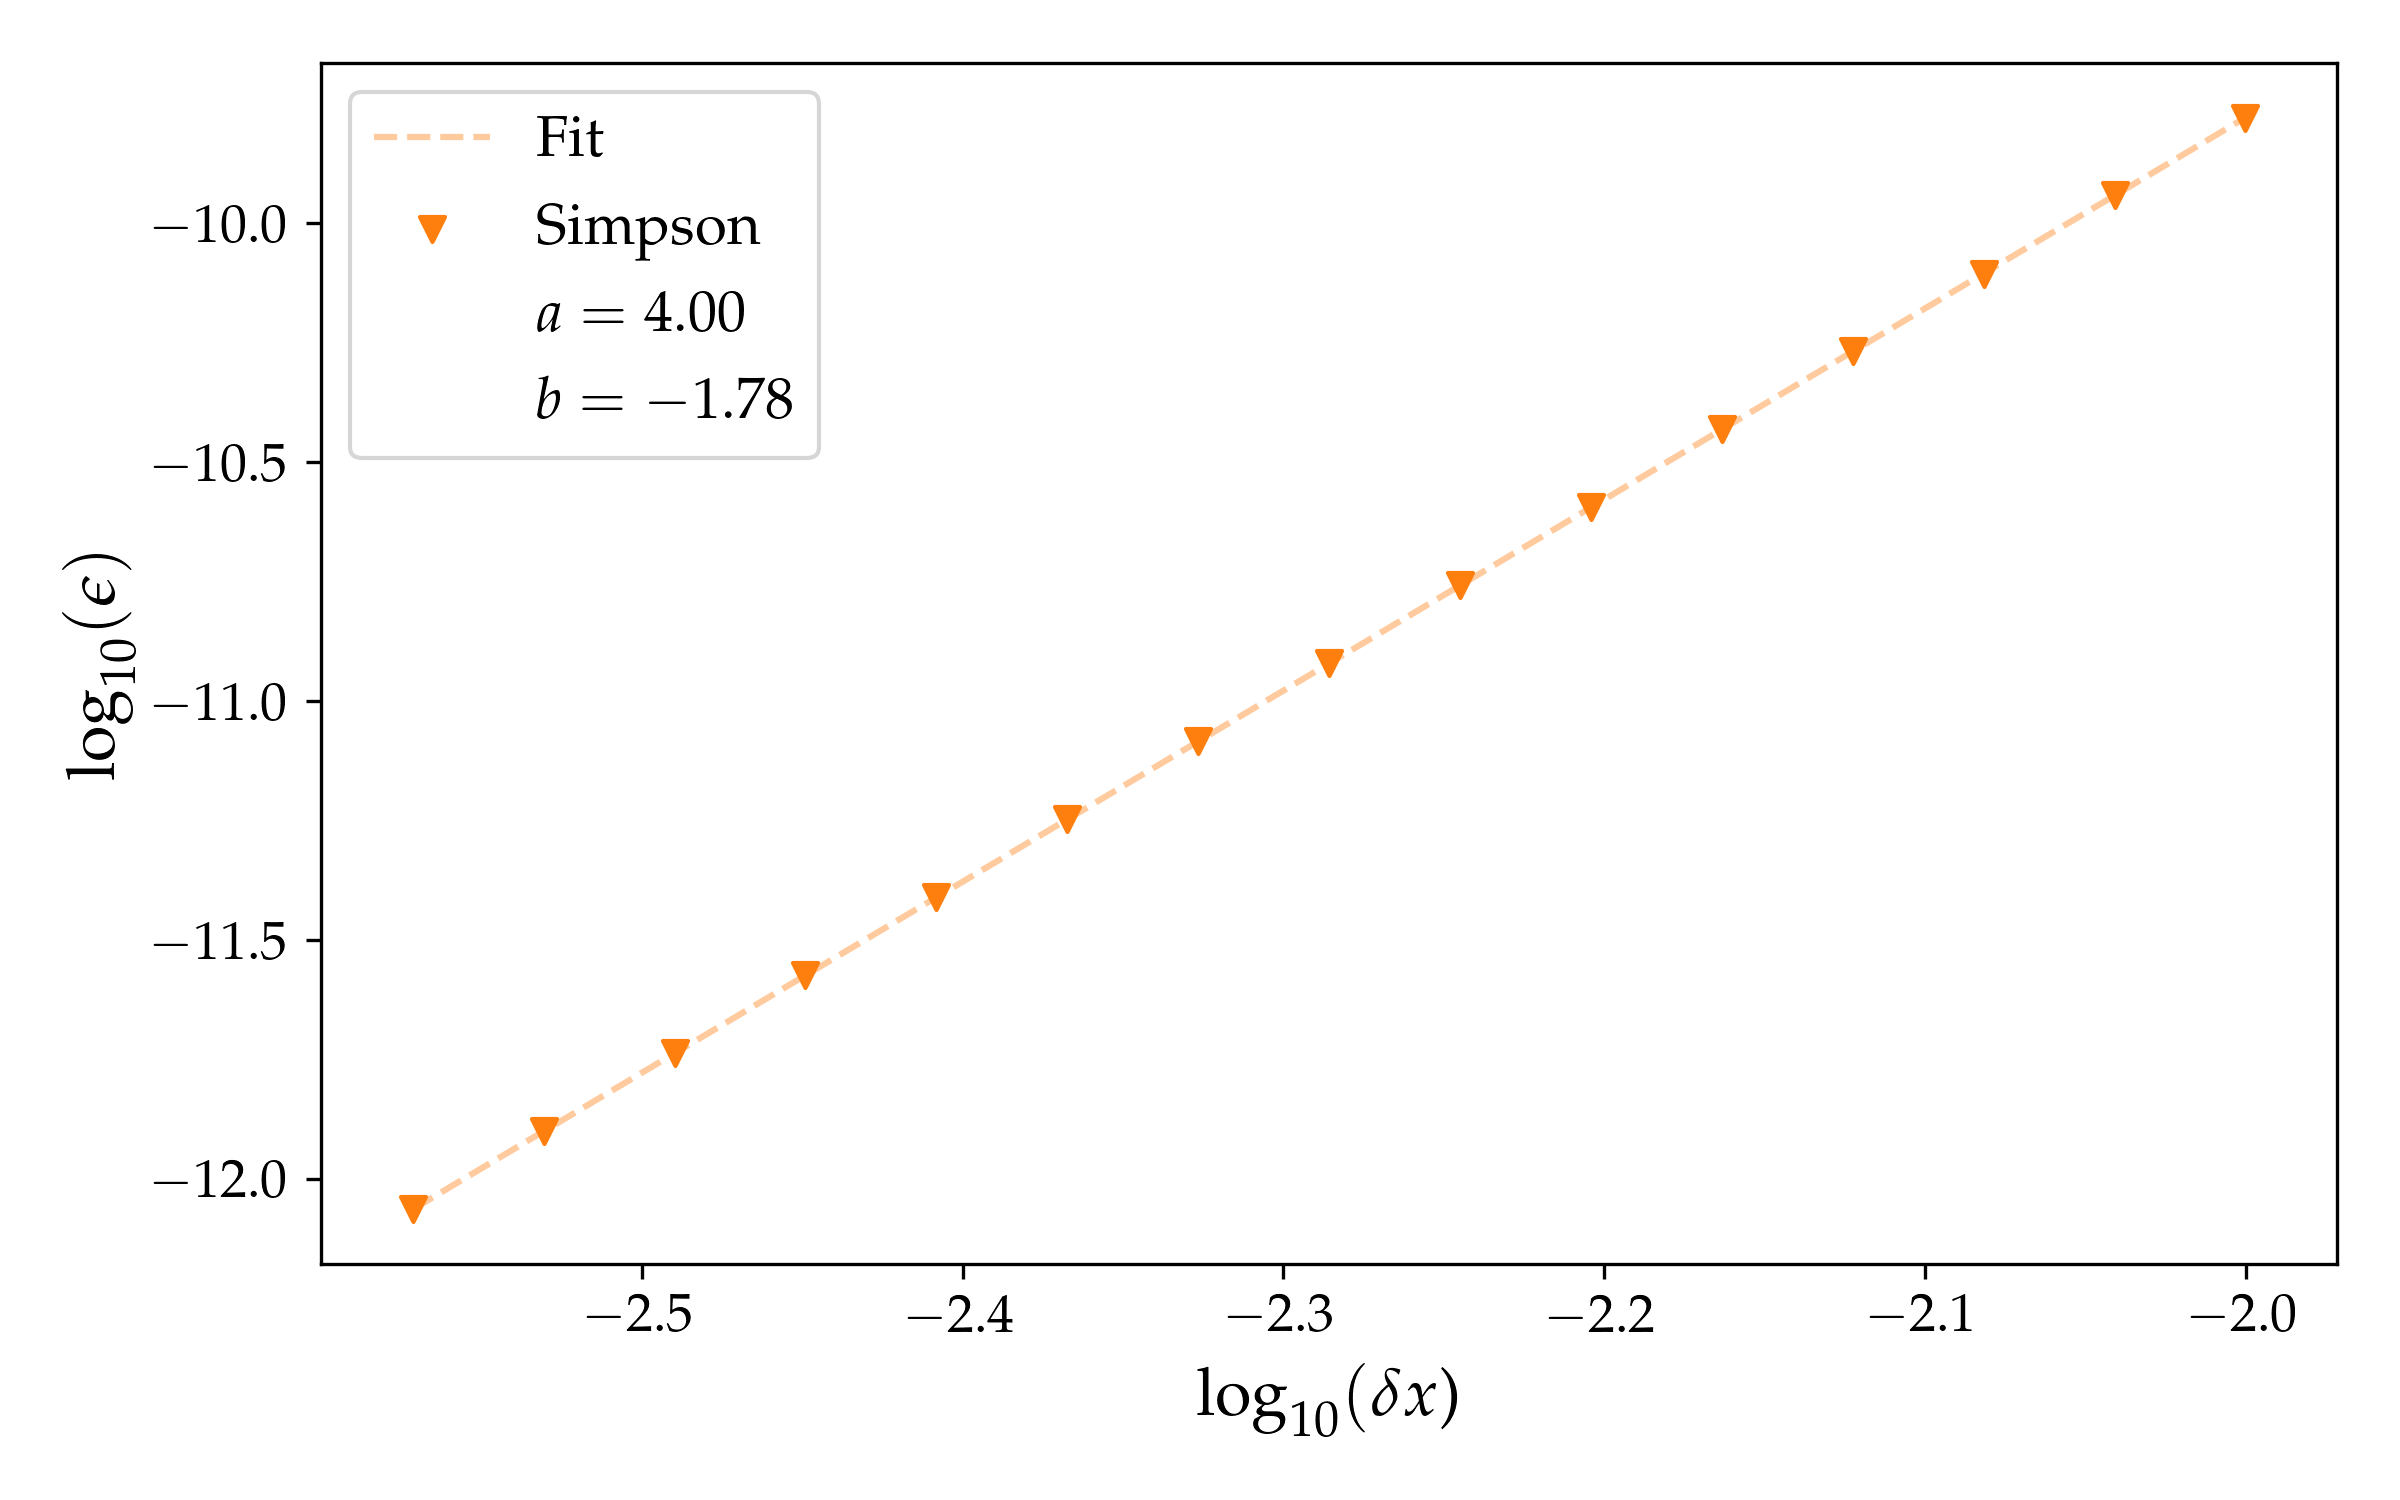
\includegraphics[width=0.8\linewidth]{images/20/Fit_gl_simp.png}
    \caption{Fit sulla Regola di Simpson composta in funzione del passo $\delta x$.}
    \label{fig: fit_simp_glob}
\end{figure}

\begin{figure}[H]
    \centering
    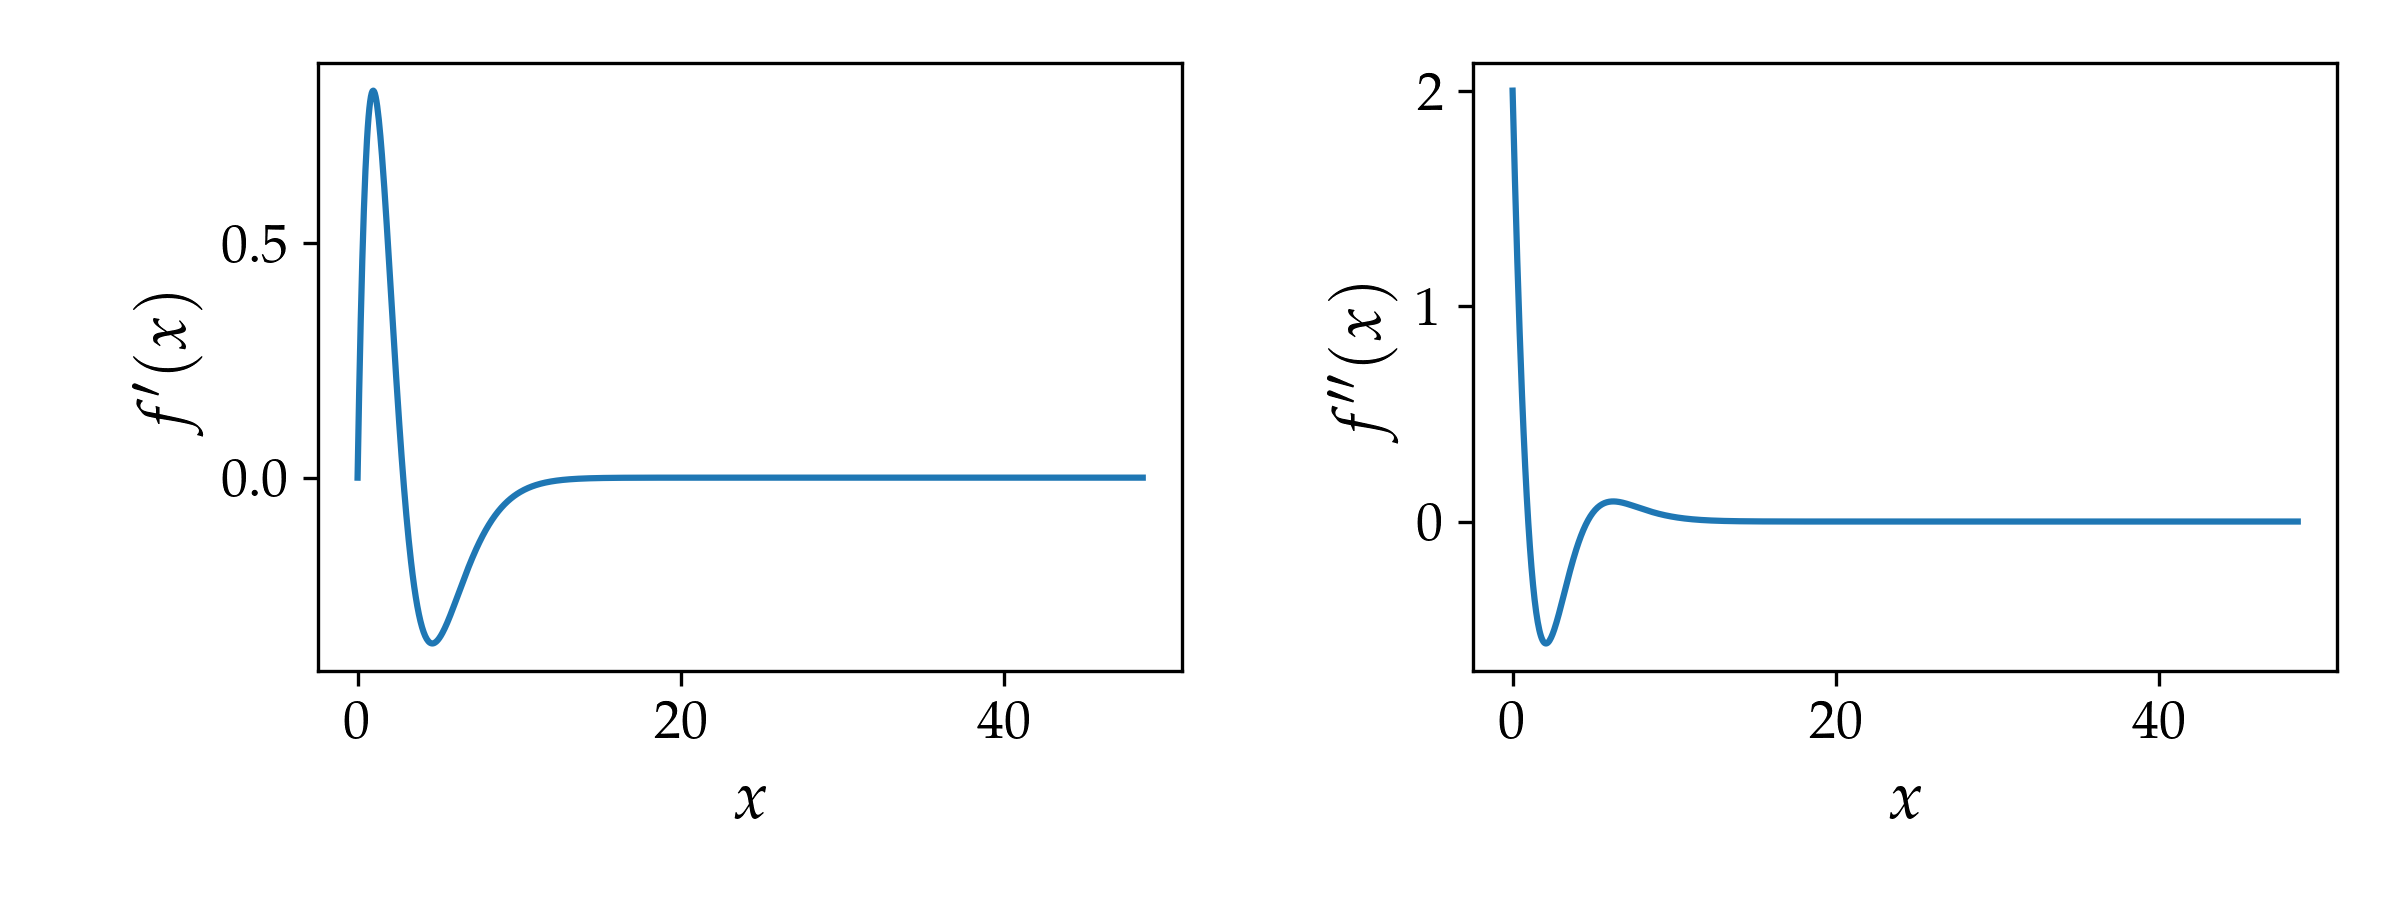
\includegraphics[width=\linewidth]{images/20/der_conf.png}
    \caption{Visualizzazione e confronto della derivata prima e seconda della funzione. Si può verificare che la prima si annulla agli estremi: $f'(0) =f'(x_{max}) = 0$.}
    \label{fig: der_conf}
\end{figure}

\newpage

















\section{Esercizio 8.2.1}
\subsection{Problem Statement}
Si consideri l'integrale
\[
\int_{0}^{1} \frac{4}{1 + x^2} \, dx = \pi
\]
e si studi l'accuratezza della soluzione in funzione di $\Delta x$ per la regola dei trapezi, la regola di Simpson e la quadratura di Gauss-Legendre a 2 punti. Utilizzando la conoscenza analitica dell'andamento dell'errore, si predica (per tutti i metodi) per quale valore di $N$ l'errore assoluto è pari a $10^{-6}$ e lo si verifichi con i dati.


\subsection{Premessa Teorica}
Se per gli algoritmi che abbiamo discusso in precedenza, per l'integrazione numerica, la suddivisione dell'intervallo era uniforme, possiamo scegliere questi punti in maniera più oculata.\\
Non tutti gli intervalli contribuiscono allo stesso modo al calcolo; l'introduzione di pesi e posizioni ben specifiche permette di aumentare la precisione e diminuire il numero di valutazioni della funzione.

\subsection{Metodi Numerici e Algoritmi}

La quadratura di Gauss-Legendre a 2 punti è una tecnica di integrazione numerica che ottimizza la posizione dei nodi di campionamento per massimizzare il grado di precisione del metodo, superando le limitazioni dei metodi a punti equidistanti come quelli di Newton-Cotes.

Per un dato intervallo $[x_0, x_0 + \delta x]$, l'integrale è approssimato come:
\begin{equation*}
    \int_{x_{0}}^{x_{0}+\delta x}dx~f(x) \approx \frac{\delta x}{2}[f(x_{+})+f(x_{-})]
\end{equation*}
dove i nodi di valutazione sono definiti dalla relazione:
\begin{equation*}
    x_{\pm} = x_0 + \frac{\delta x}{2} \left( 1 \pm \frac{1}{\sqrt{3}} \right)
\end{equation*}

Il metodo presenta la caratteristica di utilizzare solo due valutazioni della funzione: garantisce un'accuratezza paragonabile alla regola di Simpson, ma richiedendo un numero inferiore di valutazioni ($2$ rispetto a $3$), con un vantaggio computazionale del $33\%$.

\noindent L'algoritmo deriva dalla scelta dei nodi come radici del polinomio di Legendre di secondo grado, $P_2(x) = \frac{1}{2}(3x^2 - 1)$, la cui proprietà di ortogonalità garantisce l'annullamento dei termini di ordine superiore nell'espansione di Taylor dell'integrando.

\newpage
\subsection{Risultati e Discussione}

In primis valutiamo con i differenti metodi il valore dell'integrale, verificando la validità degli stessi; si controlla anche l'errore assoluto rispetto al valore vero di $I=\pi$.


\begin{elegantcode}
a = 0
b = 1
True = 3.141592653589793


Trapezi:

I_t = 3.141592653573126
diff = 1.66671121348827e-11


Simpson:

I_s = 3.141592653589794
diff = 8.881784197001252e-16


Gauss-Legendre: 

I_g = 3.1415926535897936
diff = 4.440892098500626e-16
\end{elegantcode}


\bigskip\noindent
Seguendo le indicazioni della consegna, desideriamo studiare e predire, per ciascun metodo, per quale valore di $N$ l'errore si assesti sotto la soglia di $\epsilon=10^{-6}$.

\begin{figure}[H]
    \centering
    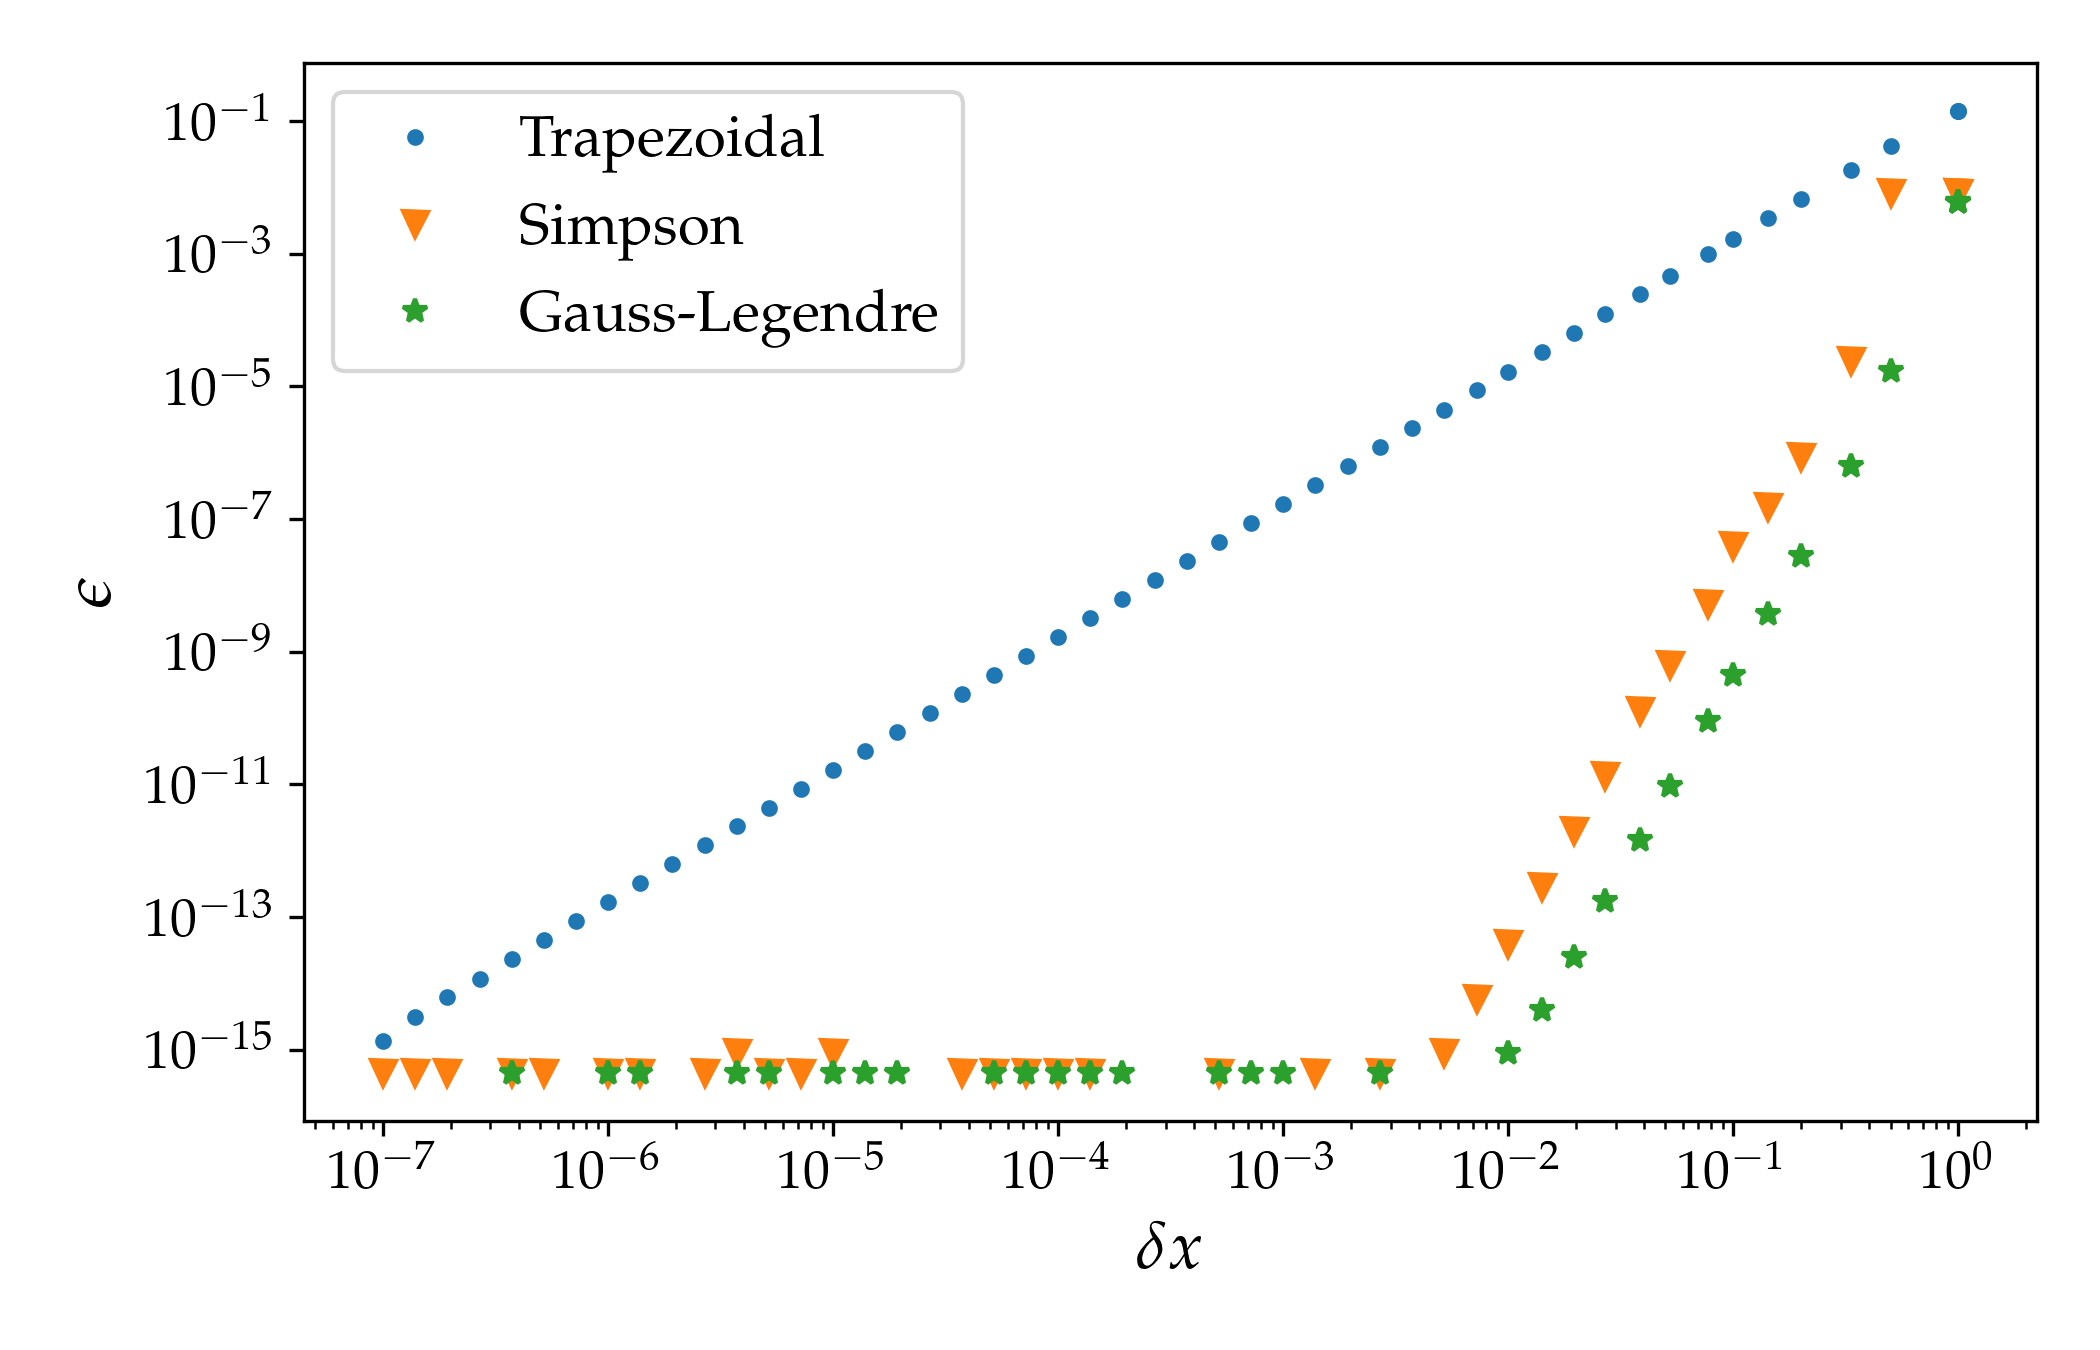
\includegraphics[width=0.8\linewidth]{images/21/conf_3mth.png}
    \caption{Confronto della convergenza tra i diversi metodi, in funzione di $\delta x$, intervallo uniforme in cui sezioniamo $I=[0,1]$.}
    \label{fig: conv_int_dx}
\end{figure}

\noindent In generale abbiamo già fatto alcune considerazioni sulla convergenza dei tre metodi, affermando che quello dei trapezi ha convergenza quadratica, mentre gli altri due quartica; in questo caso commentiamo i risultati del fit che viene fatto studiando l'errore degli algoritmi in funzione del passo $\delta x\in [10^{-7}, 1]$ (cioè proprio il loro \textit{scaling}).\\
Seguono Fig. \ref{fig: fit_trap_6} - \ref{fig: fit_Gauss_leg} per confronto.

\begin{figure}[H]
    \centering
    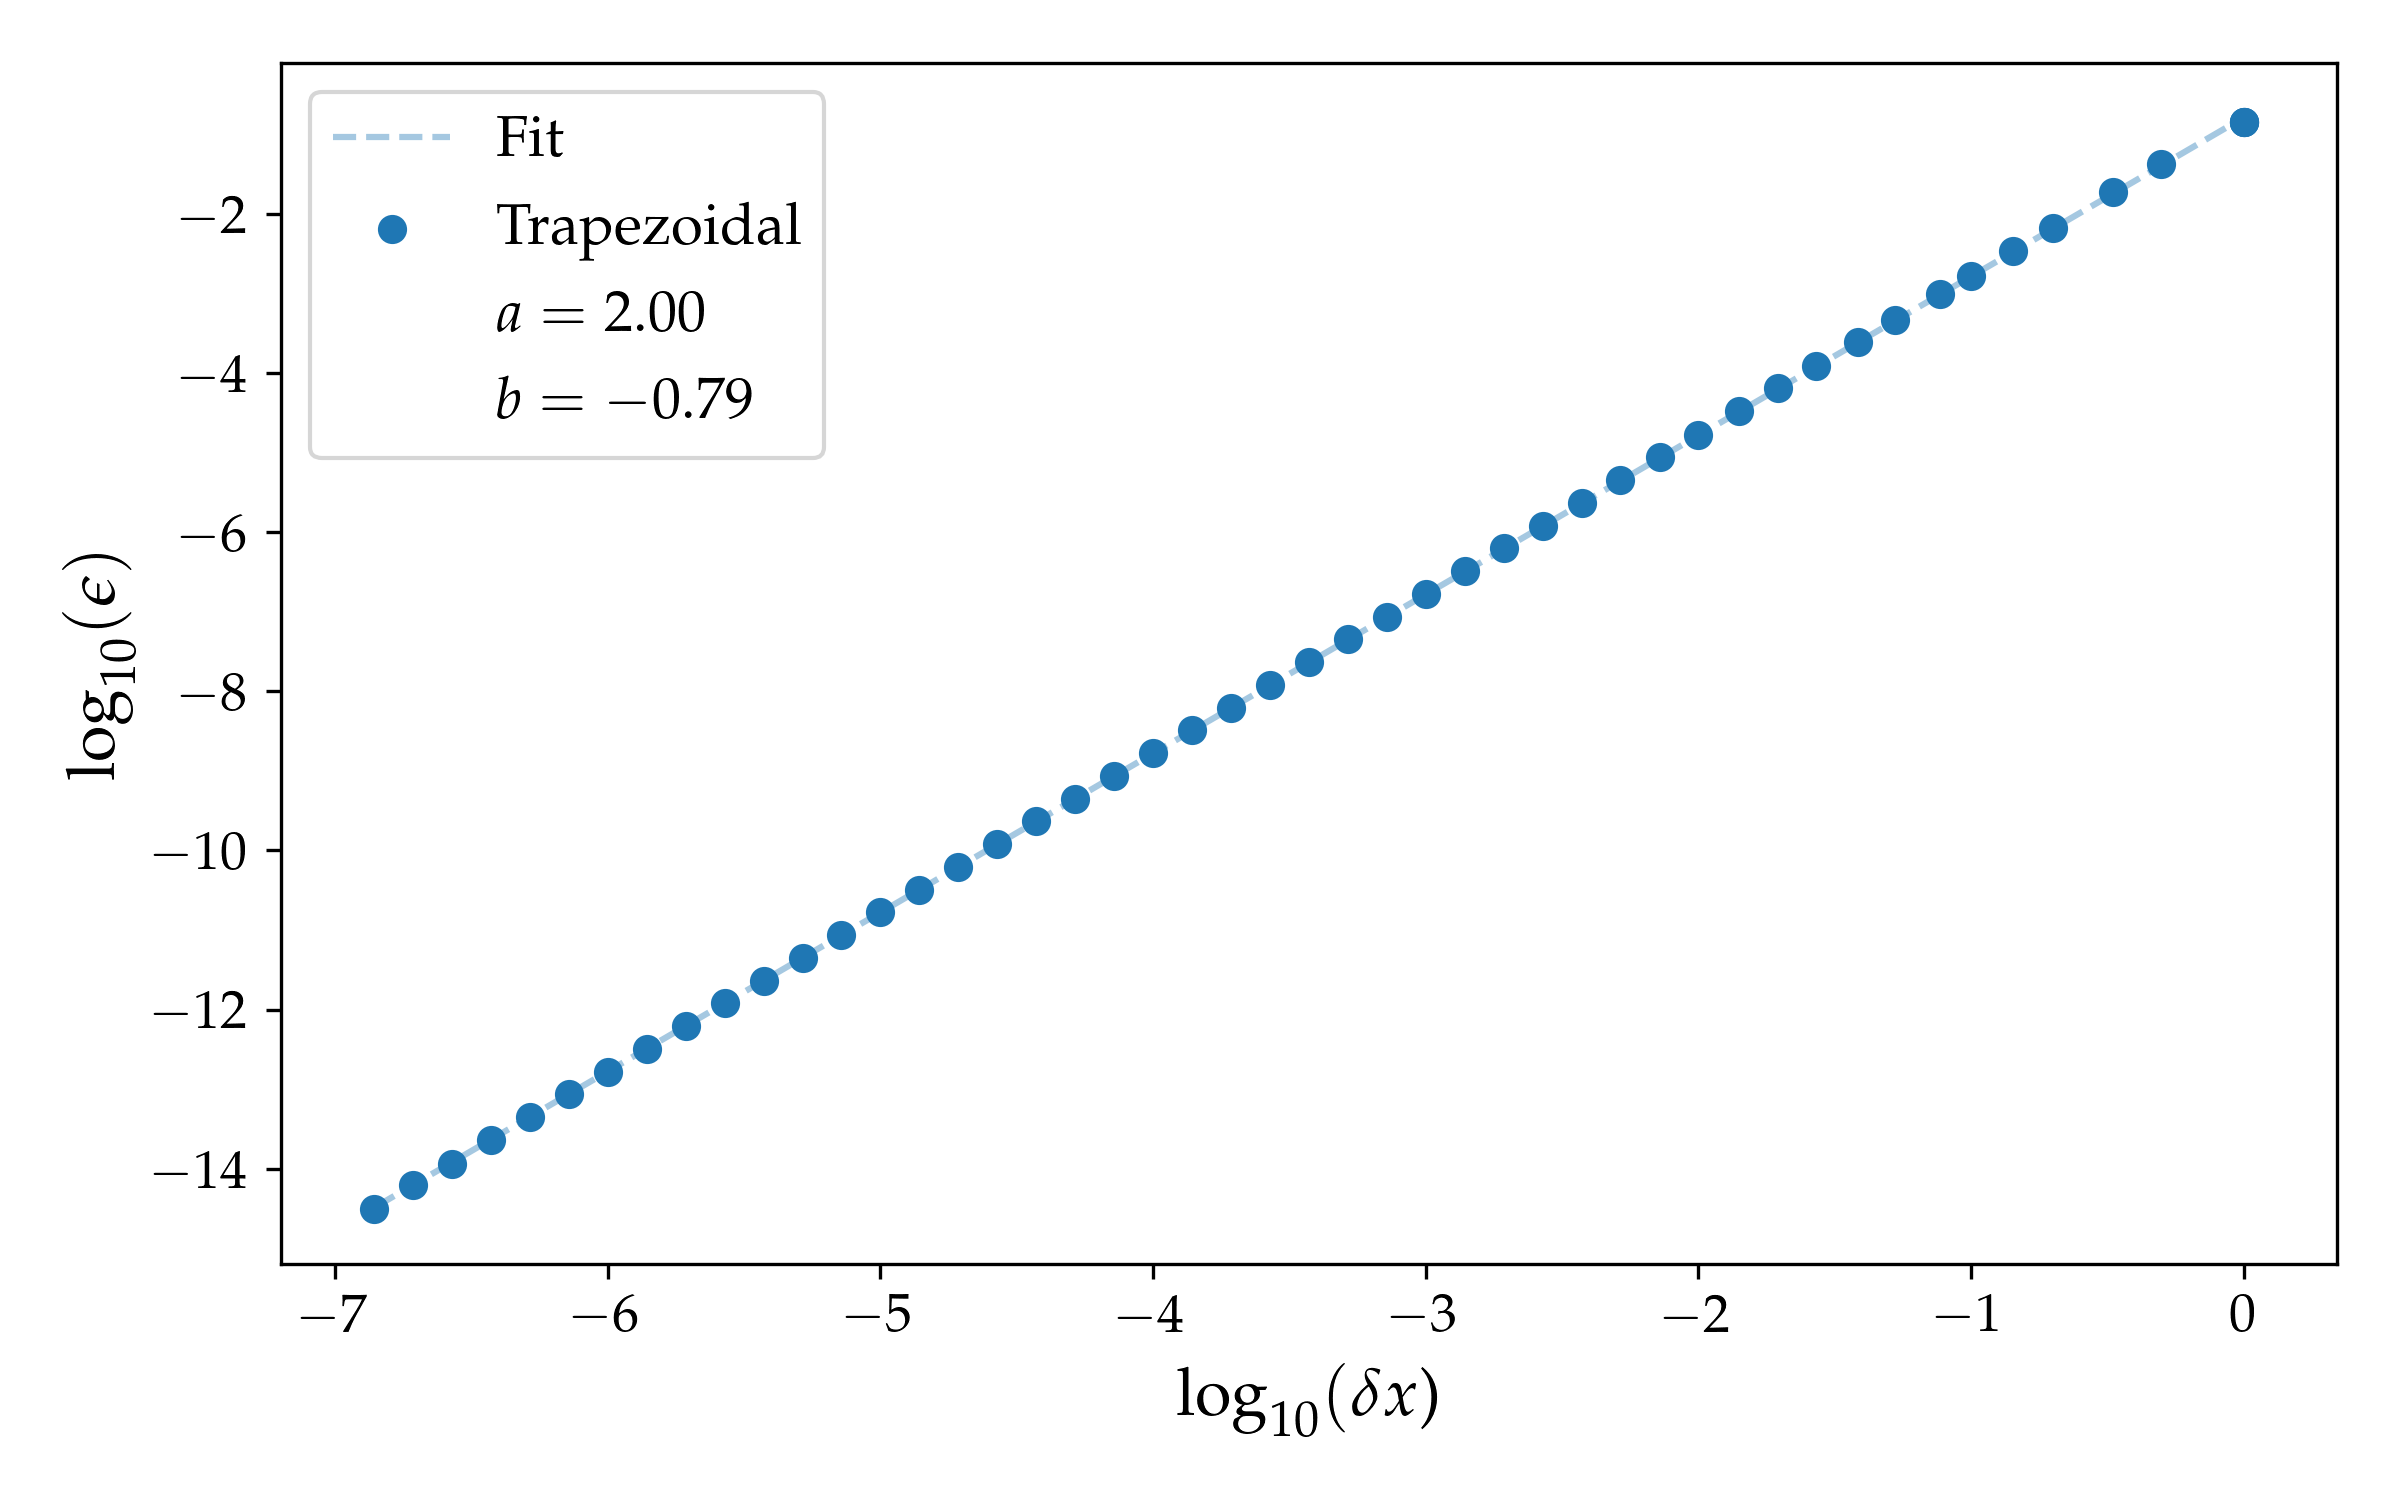
\includegraphics[width=0.8\linewidth]{images/21/FitTrap_2.png}
    \caption{Fit della convergenza del metodo dei trapezi nel caso di questo esercizio.}
    \label{fig: fit_trap_6}
\end{figure}

\begin{figure}[H]
    \centering
    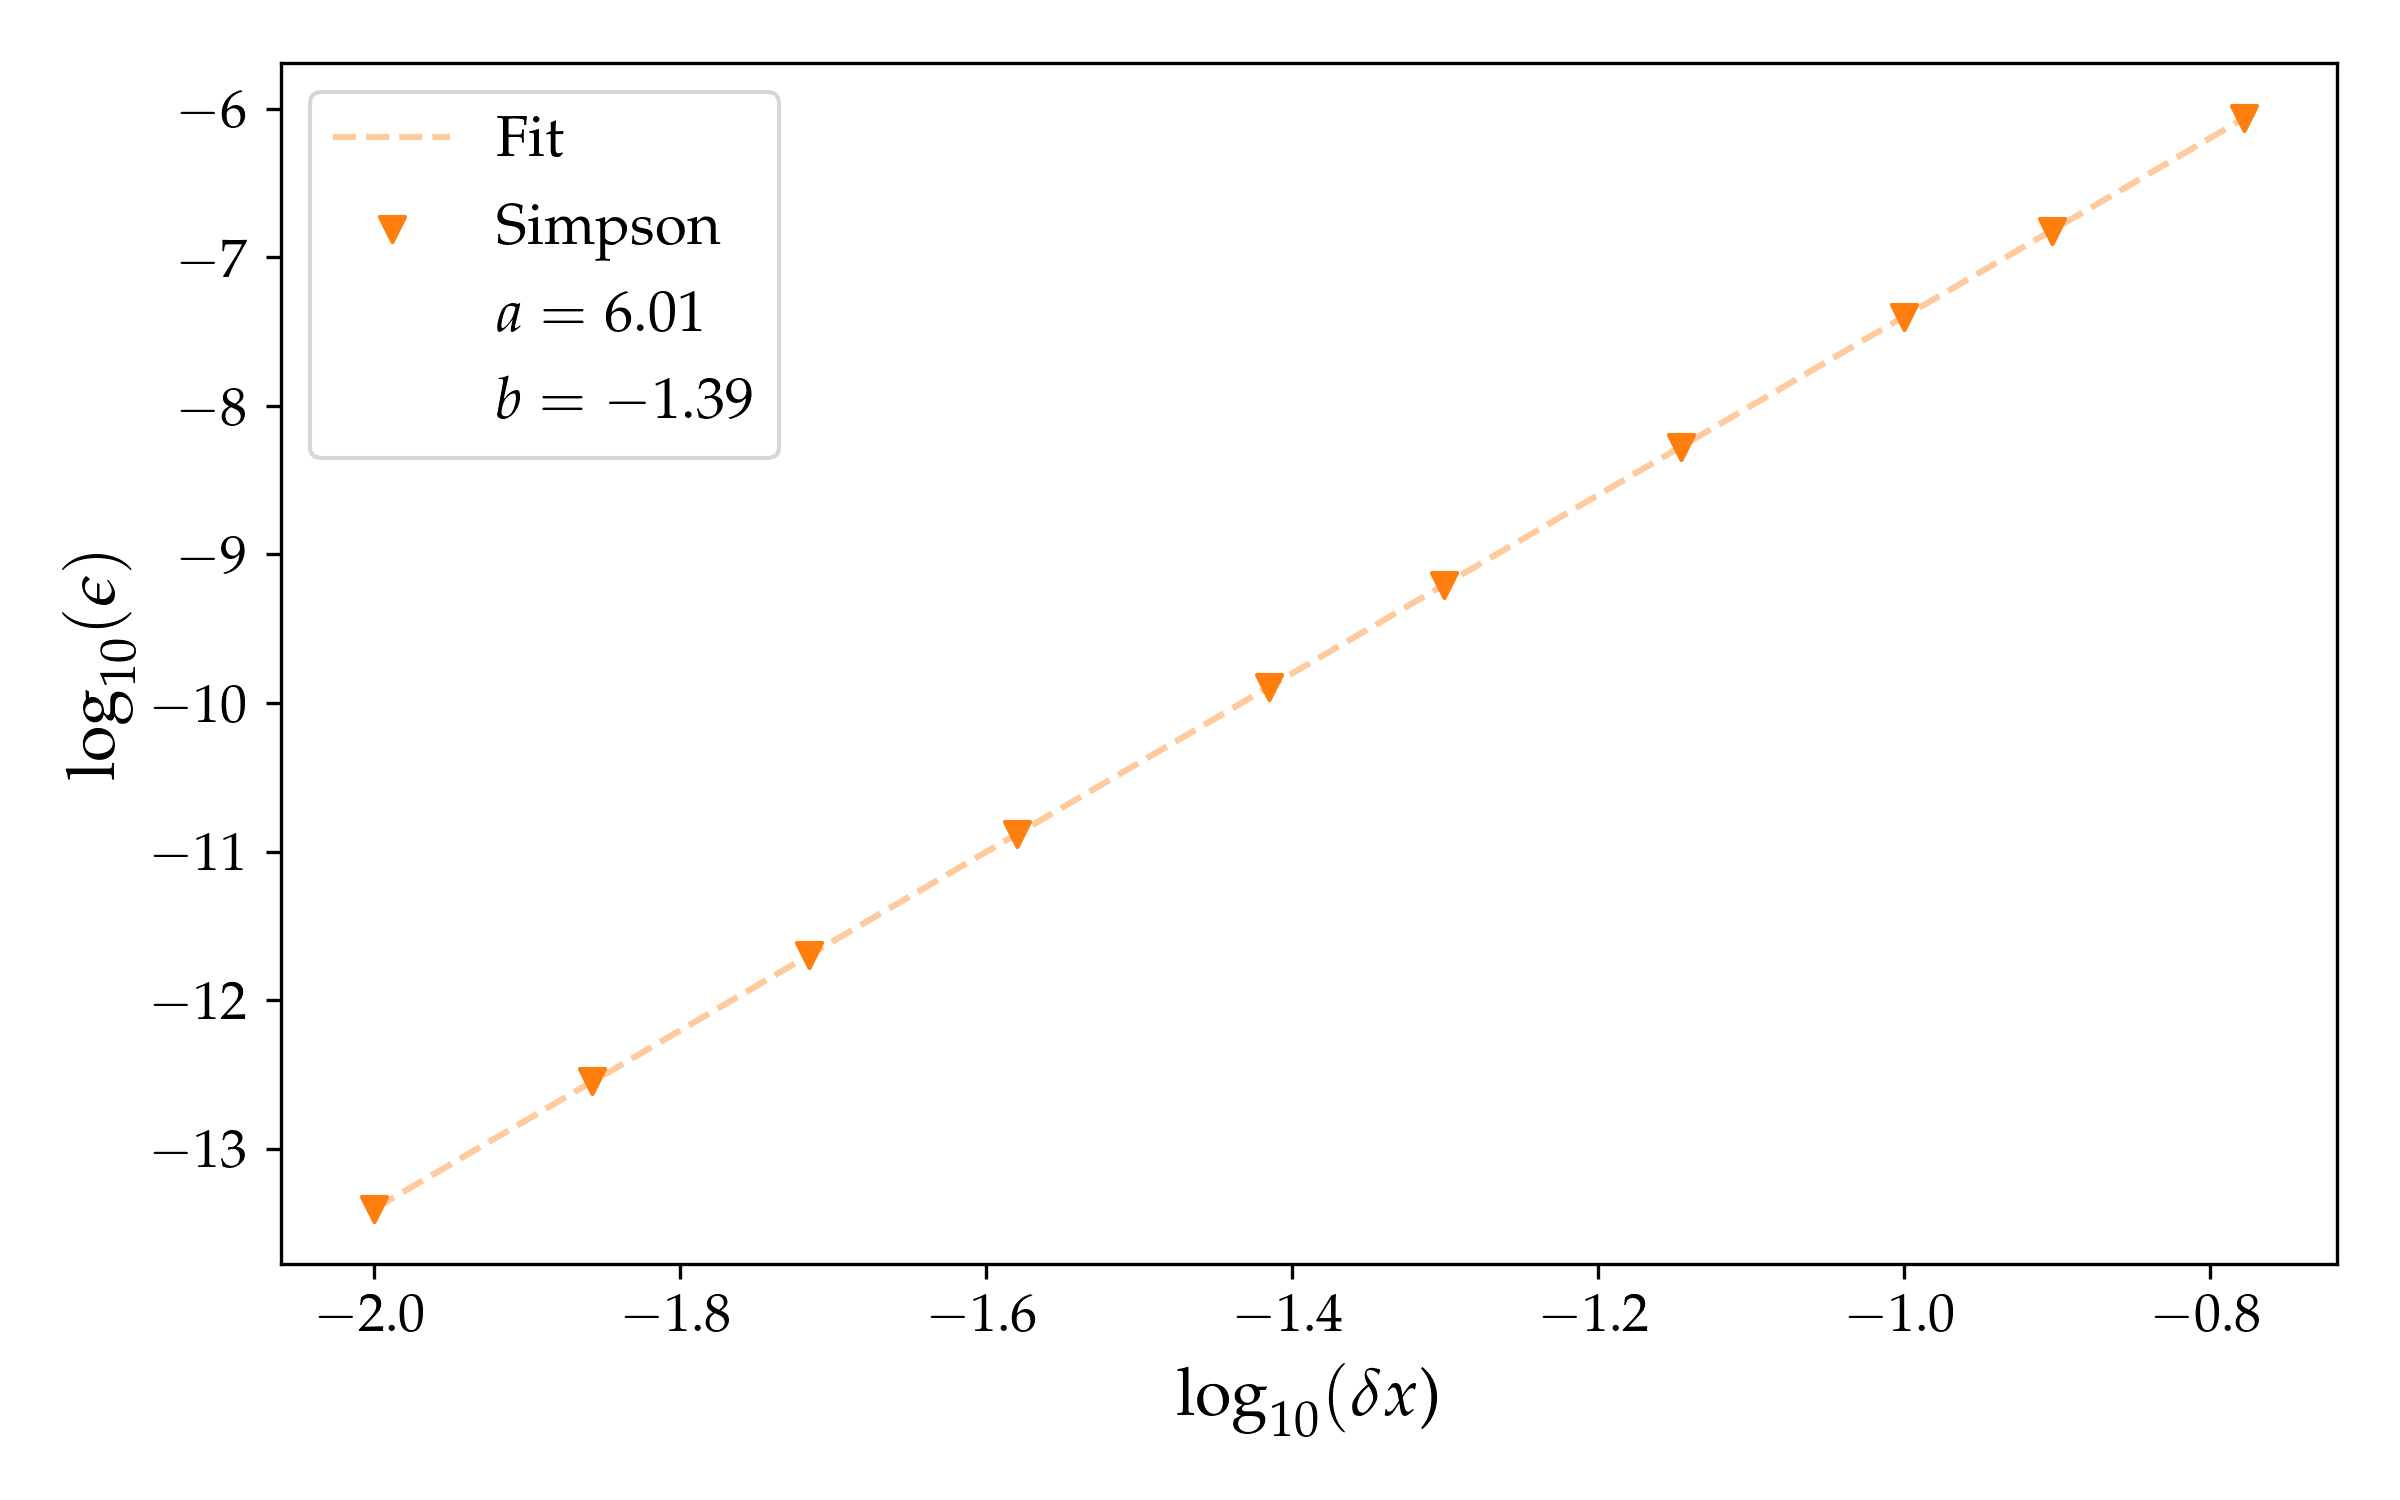
\includegraphics[width=0.8\linewidth]{images/21/FitSimp_2.png}
    \caption{Fit della convergenza del metodo di Simpson nel caso di questo esercizio.}
    \label{fig: fit_simp_6}
\end{figure}

\begin{figure}[H]
    \centering
    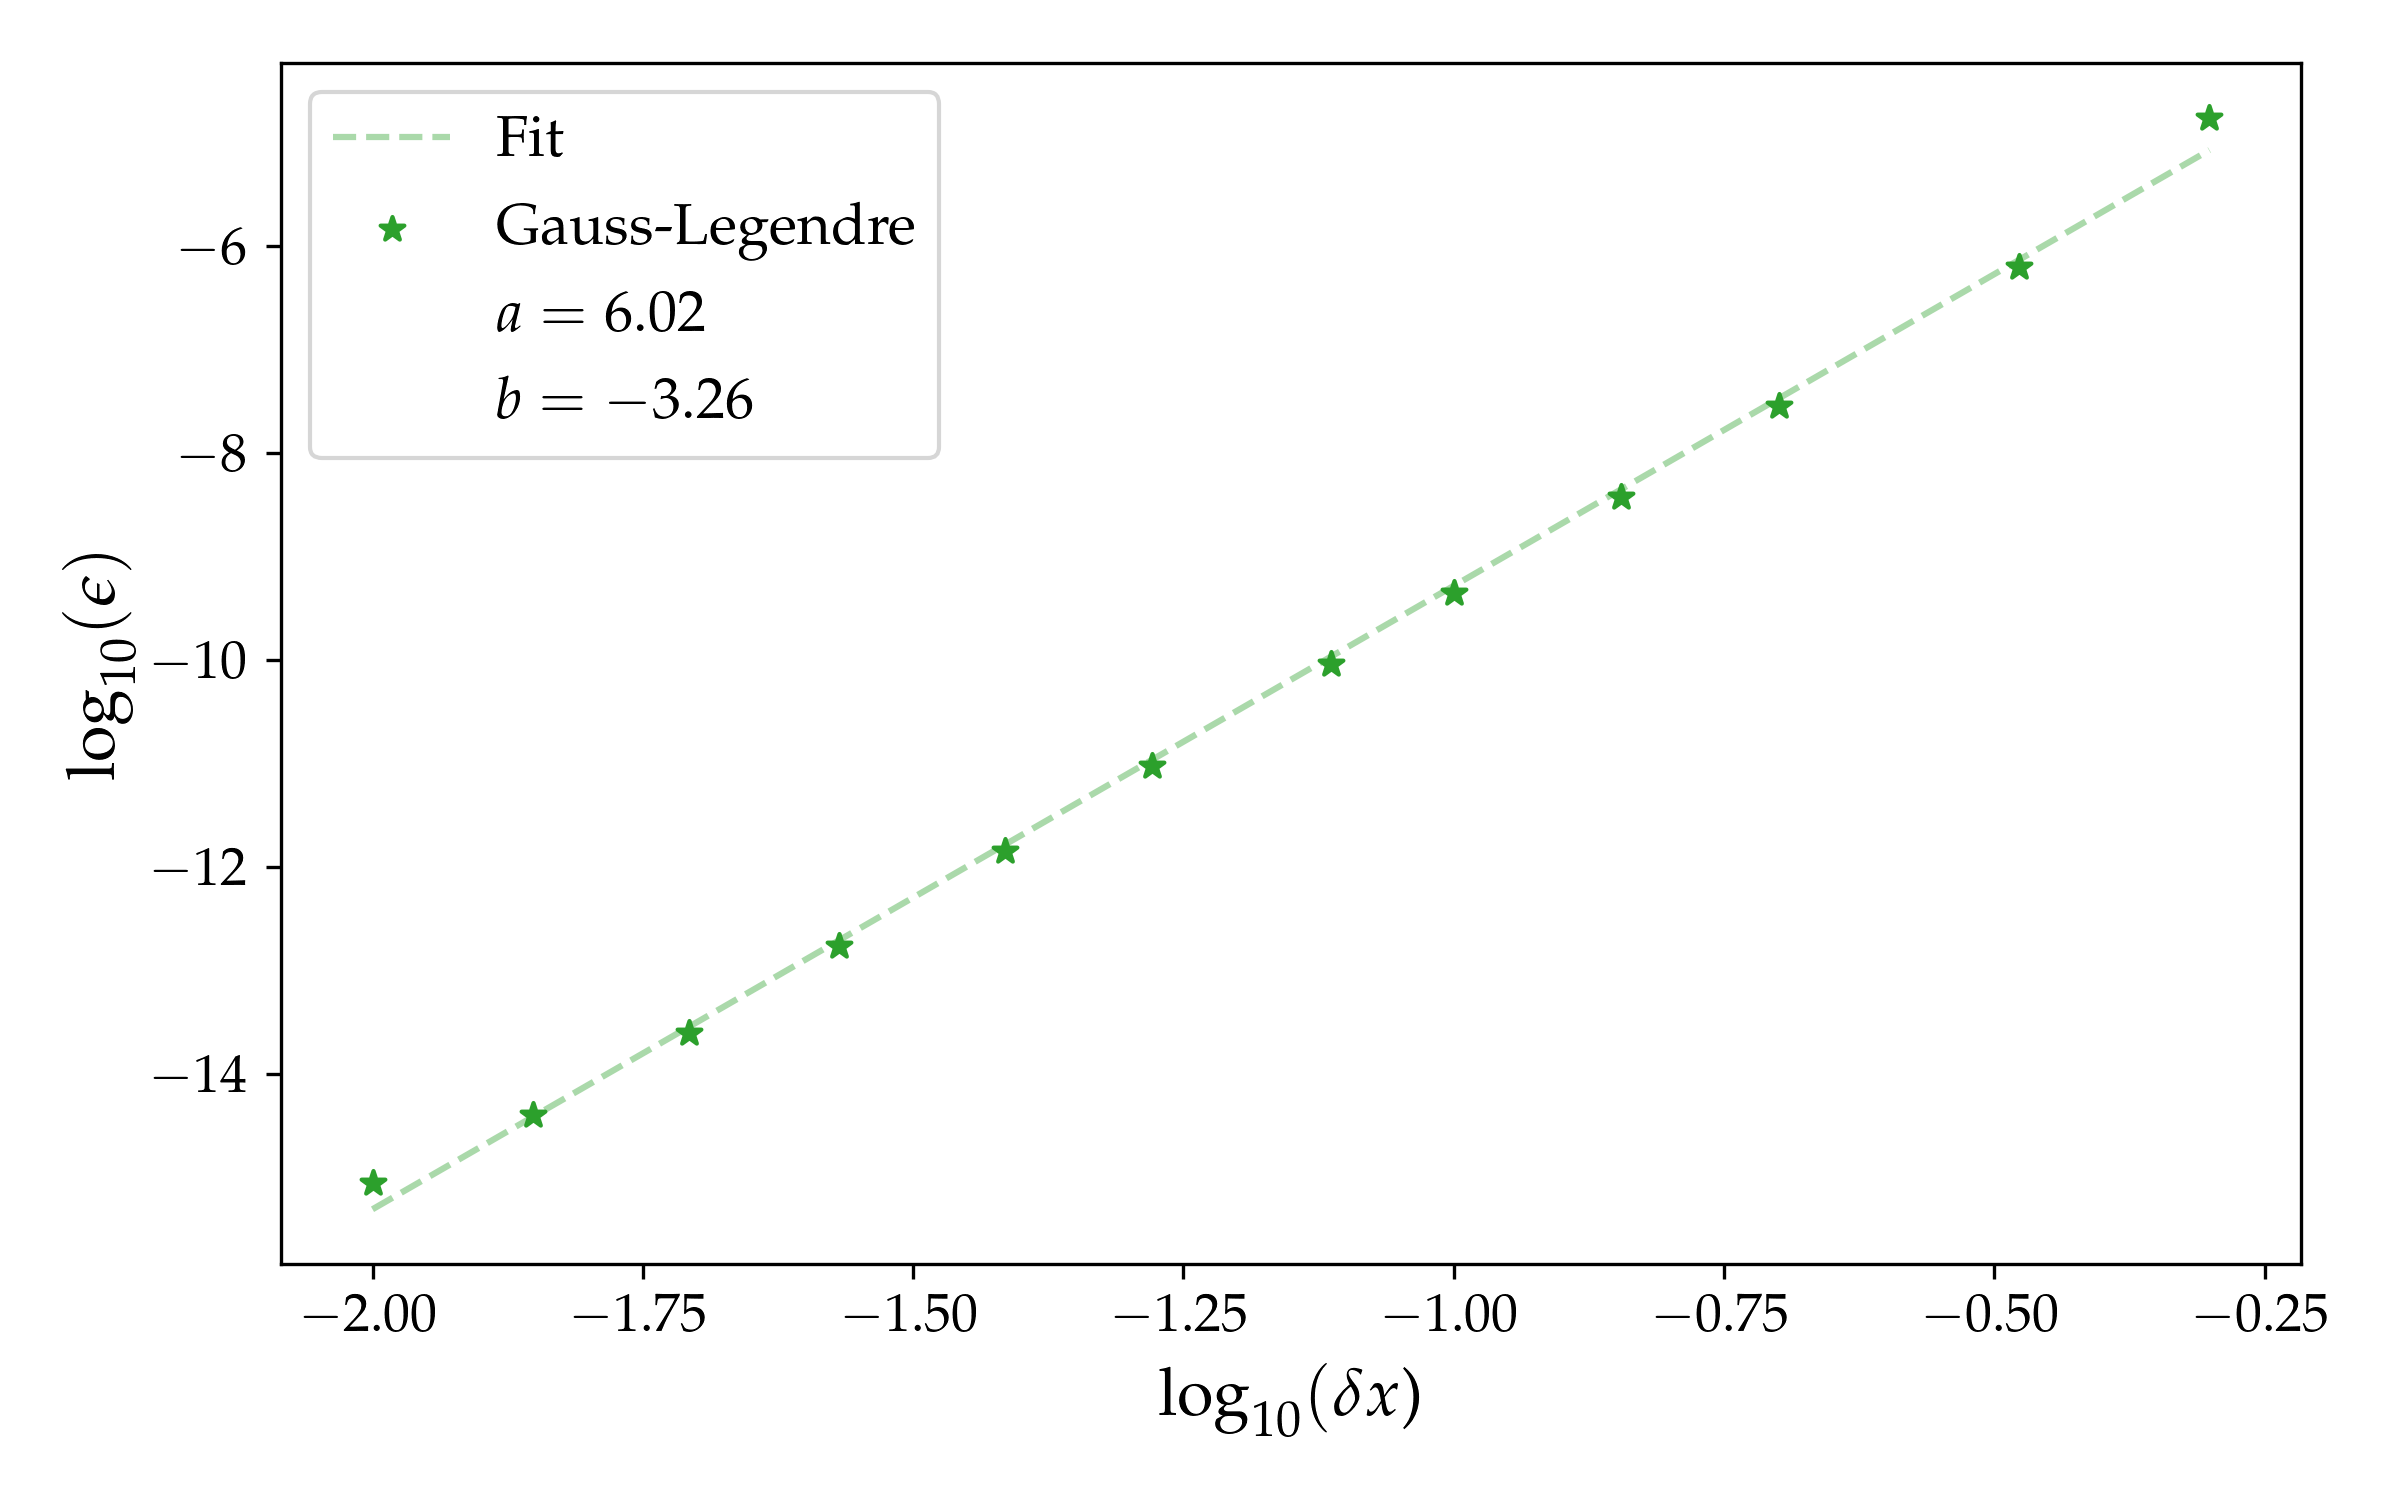
\includegraphics[width=0.8\linewidth]{images/21/FitGauss_2.png}
    \caption{Fit della convergenza del metodo della quadratura 2-punti di Gauss-Legendre nel caso di questo esercizio.}
    \label{fig: fit_Gauss_leg}
\end{figure}

\noindent L'ordine asintotico generale dei metodi rimane $p=4$; per questa particolare funzione il termine dominante dell'errore si annulla ($f^{(3)}(1) - f^{(3)}(0) = 0$), facendo emergere il termine successivo e producendo una convergenza osservata di ordine 6.\\
In maniera del tutto simile a quella dell'esercizio precedente è possibile ricavare analiticamente questo risultato, ma in questa sezione viene omesso per analogia con il sopracitato;\\
si può verificare che $f^{(5)}(b)-f^{(5)}(a)=60$, cioè che il primo termine non nullo sia quello di grado sei (le potenze dispari si annullano, a cui sono associate derivate pari).

\bigskip\noindent Possiamo quindi procedere a ricavare una stima per il numero $N$ di intervalli necessari per ottenere una determinata precisione. Se guardiamo il \textit{leading order} vale che:
$$\epsilon_G(\delta x) = O(\delta x^p) \approx k\ {\delta x}^p \Delta f^{(p-1)}$$
$$k\in \mathbb{R},\ \delta x = \frac{|b-a|}{nN}=\frac{1}{nN}, \ \Delta f ^{(p-1)} = |f^{(p-1)}(b) - f^{(p-1)}(a)|$$

\noindent Dove $n$ è un parametro proprio del metodo, per esempio $n=1$ implica che $\delta x$ sia la larghezza dell'intervallo che otteniamo dividendo in $N$ sottointervalli $b-a$, $n=2$ implica che equivalga al doppio di questa lunghezza, così procedendo.\\
Imponiamo che sia $\epsilon_G\le\varepsilon_{tol}=10^{-6}$.

\begin{align*}
    \epsilon_G &= \frac{k\ \Delta f^{(p-1)}}{n^p N^p}\le \varepsilon_{tol}\\
    \\
    N &\ge \frac{1}{n}\left(\frac{k}{\varepsilon_{tol}}\Delta f ^{p-1}\right)^{1/p}
\end{align*}

\newpage
\begin{itemize}
    \item \textbf{Trapezi}: $n=1$
    $$\epsilon_G \approx \frac{1}{12} \frac{1}{ N^2}\Delta f' = O(N^{-2})  \implies k=\frac{1}{12},\ p=2$$
    
    \item \textbf{Simpson}: $n=2$
    $$\epsilon_G \approx \frac{1}{3780} \frac{1}{N^6}\Delta f^{(5)} = O(N^{-6})  \implies k=\frac{1}{3780},\ p=6$$
 
    \item \textbf{Gauss-Legendre}: $n=1$ 
    $$\epsilon_G \approx \frac{1}{435456} \frac{1}{N^6} \Delta f^{(5)} = O(N^{-6})  \implies k=\frac{1}{435456},\ p=6$$
    
    
\end{itemize}



\bigskip\noindent

Di seguito un riassunto che ricapitola tutti i risultati raccolti
\begin{elegantcode}
Expected = 2
    p_t = 1.9970176429343596

Expected = 4
    p_s = 6.0067049348684565
    p_g = 6.0223475927006165

------------------ check ------------------

d3f(1) - d3f(0) = (-0.0) - (-0.0) = 0.0
d5f(1) - d5f(0) = (60.0) - (0.0) = 60.0

-------------------------------------------

- if Trapezoidal, p = 2, n = 1, k = 1/12:
     N = 409

- if Simpson, p = 6, n = 2, k = 1/3780:
     N = 4

- if Gauss-Legendre, p = 6, n = 1, k = 1/435456:
     N = 3
\end{elegantcode}


\bigskip\noindent Ciò che confermiamo è la gerarchia nella convergenza al valore vero dei diversi metodi, cioè possiamo mostrare come il trapezio viaggi a ordini di distanza rispetto agli altri due metodi, come velocità e costo computazionale, ma inoltre tra i due simili (entrambi quartici nella formulazione generale) la quadratura di Gauss-Legendre a 2 punti raggiunge la precisione richiesta con un numero inferiore di sottointervalli rispetto agli altri metodi, grazie anche al coefficiente numerico del termine dominante dell'errore.\\
Il grafico che segue, in Fig. \ref{fig: confr_Ndep}, rappresenta chiaramente proprio questo fenomeno, conferma le nostre ipotesi analitiche e le valutazioni fatte fino a questo momento: possiamo osservare che la \textit{treshold} fissata a $10^{-6}$ dell'errore è raggiunta dai metodi in corrispondenza delle soglie che abbiamo fissato con i nostri risultati. 

\begin{figure}[H]
    \centering
    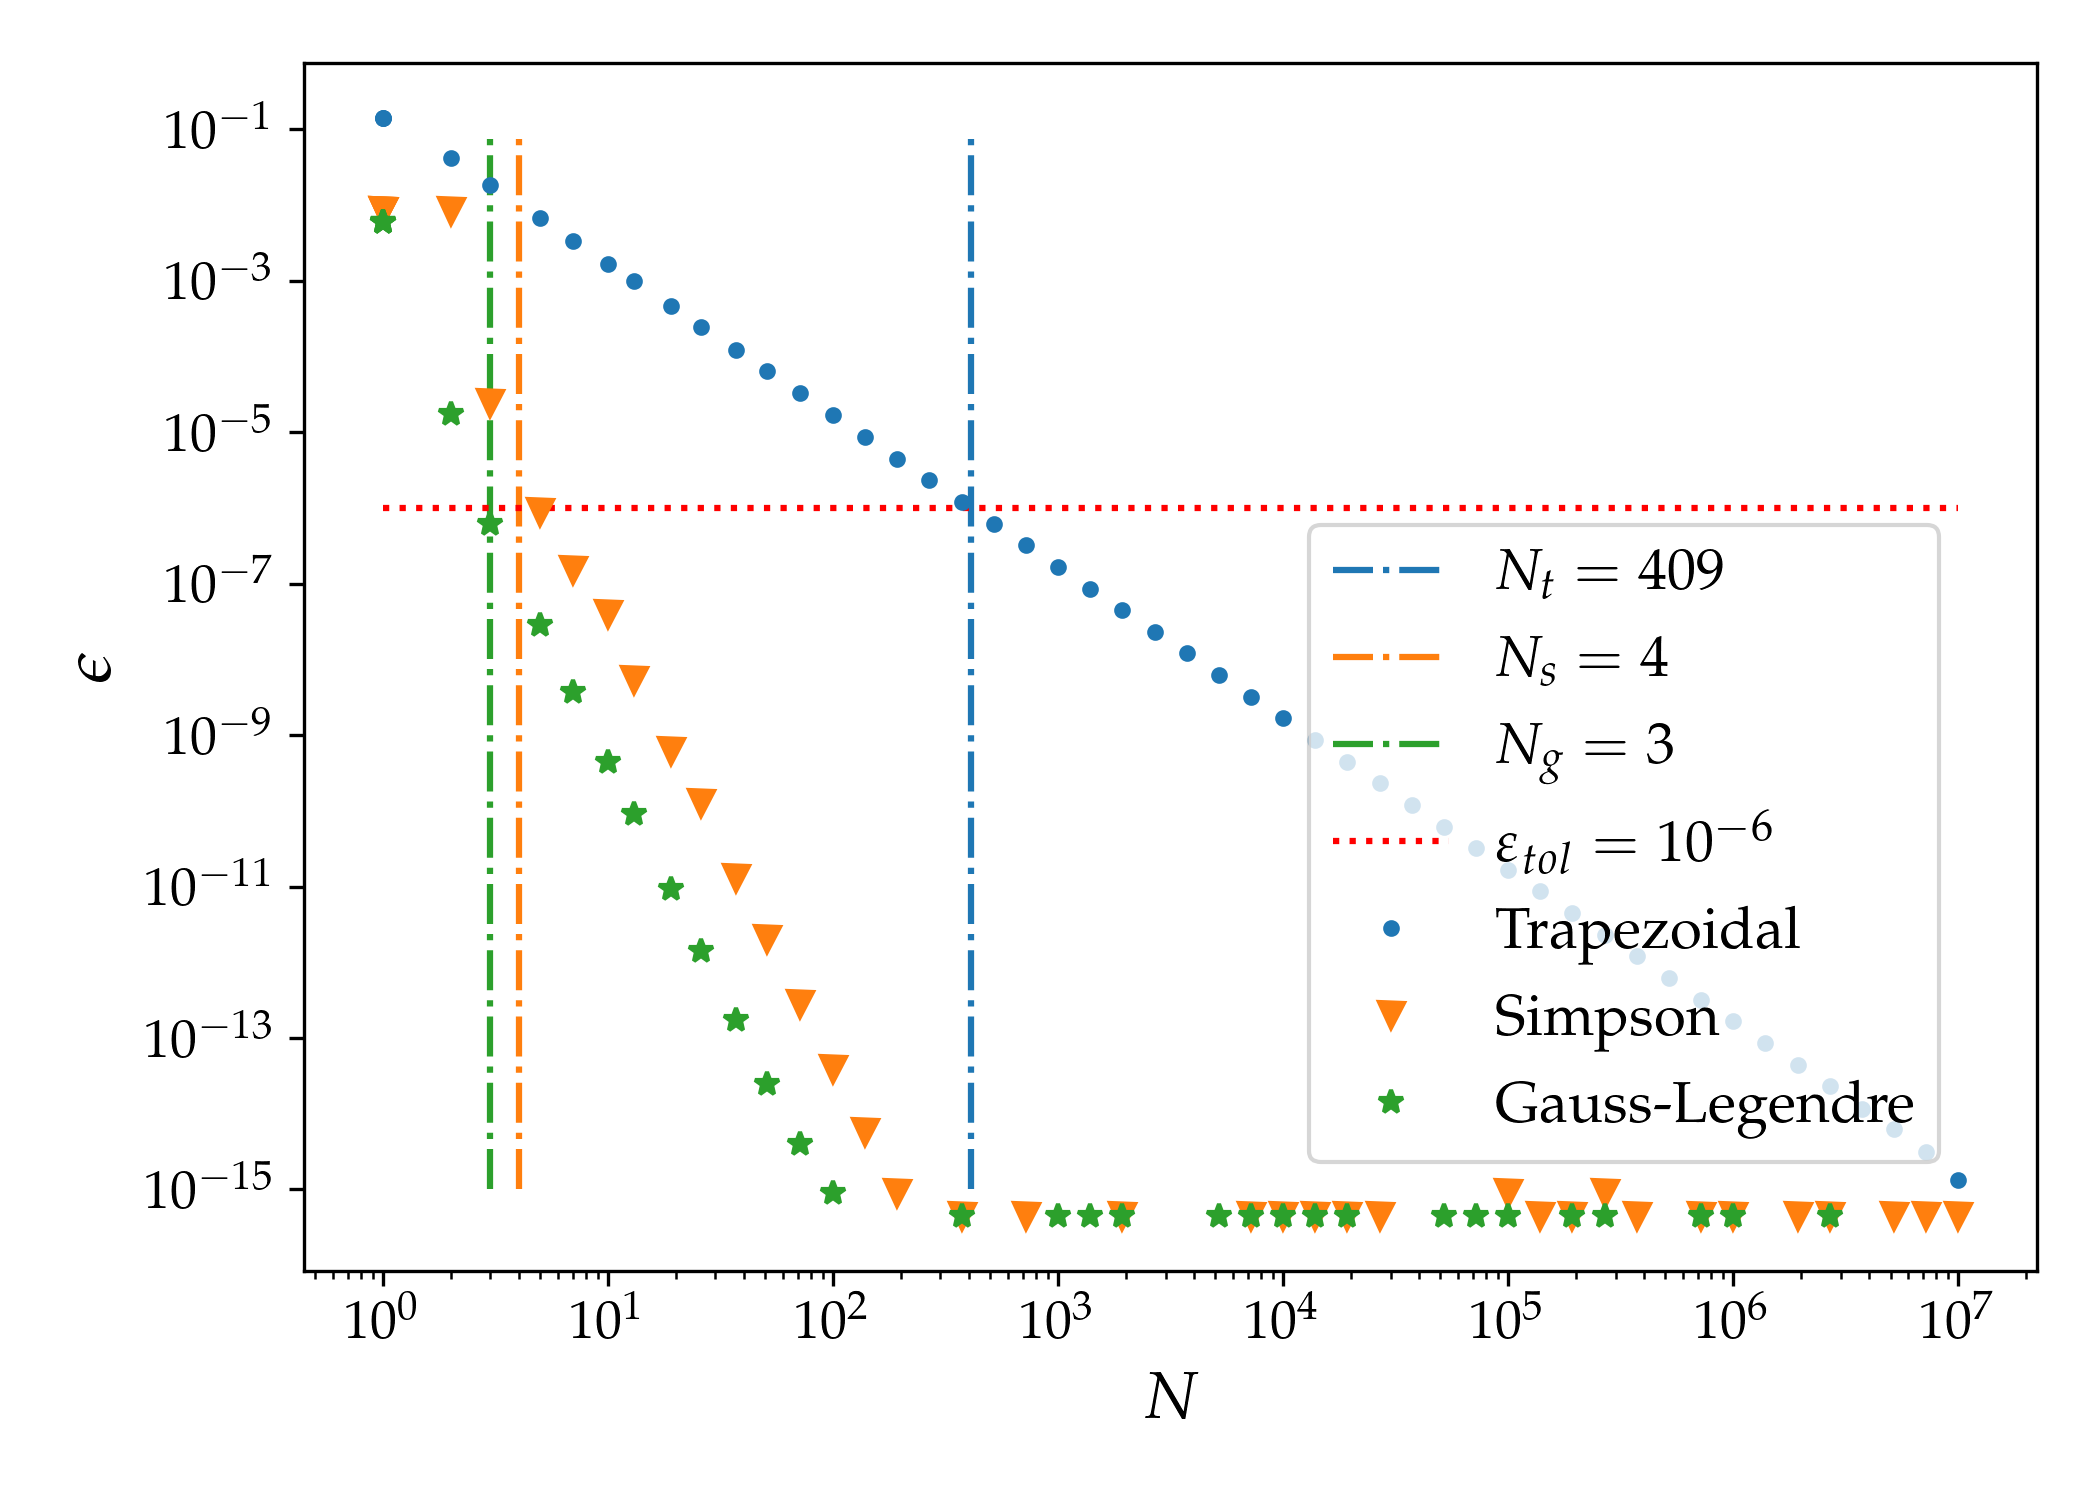
\includegraphics[width=0.8\linewidth]{images/21/check_prev.png}
    \caption{Confronto della convergenza tra i diversi metodi, in funzione di $N$, numero di intervalli in cui suddividiamo $I = [0,1]$.}
    \label{fig: confr_Ndep}
\end{figure}

\noindent L'ulteriore verifica che propongo passa attraverso il calcolo numerico dell'errore ($\epsilon =|I_{true} - I_{mth}|$) in funzione del numero di intervalli determinato: si confronti con il valore di riferimento di $\varepsilon_{tol}=10^{-6}$

\begin{elegantcode}
TRAPEZOIDAL:
   e = 9.96e-07

SIMPSON:
   e = 1.51e-07

GAUSS-LEGENDRE:
   e = 6.21e-07

\end{elegantcode}

\newpage











\section{Esercizio 8.2.2}
\subsection{Problem Statement}
Per i polinomi di Hermite $H_n$, la condizione di ortogonalità è

$$(H_n, H_m) = \sqrt{\pi} 2^n n! \delta_{nm}$$


Essi soddisfano la relazione


$$H_{n+1}(x) = 2xH_n(x) - 2nH_{n-1}(x), \quad H_0(x) = 1, \quad H_{-1}(x) = 0$$


Scrivere un programma che, data una funzione $f(x)$ e un numero intero $n$, esegua i seguenti compiti:
\begin{enumerate}
\item Calcolare le radici del polinomio di Hermite di ordine $n$, $H_n(x)$; per questo compito, riutilizzare il programma già scritto nella sezione relativa alle radici delle funzioni.
\item Calcolare i pesi di Gauss-Hermite $w_i$ utilizzando


$$w_i = \frac{2^{n-1} n! \sqrt{\pi}}{n^2 [H_{n-1}(x_i)]^2}$$


\item Approssimare l'integrale


$$\int_{-\infty}^{\infty} dx \, e^{-x^2} f(x) \approx \sum_{i=1}^{n} w_i f(x_i)$$


\end{enumerate}
Studiare i seguenti integrali con la quadratura di Gauss-Hermite e la loro convergenza per diversi valori di $n$:
\begin{enumerate}
\item $\int_{-\infty}^{\infty} dx \frac{e^{-x^2}}{1+x^2}$
\item $\int_{0}^{\infty} dx \, x^8 e^{-x^2}$
\item $\int_{3}^{\infty} dx \, x^5 e^{-x^2}$
\end{enumerate}
Tracciare un grafico dei pesi $w_i$ sull'asse $y$ e delle radici $x_i$ sull'asse $x$, per diversi valori di $n$ nel caso $(-\infty, \infty)$. Per l'ultimo integrale confrontare i risultati con uno studio (in funzione del numero di punti) usando la regola dei trapezi e di Simpson.

\subsection{Premessa Teorica}
In generale la formulazione che abbiamo definito per la quadratura 2 punti di Gauss-Legendre (facente uso delle radici dei polinomi ortogonali di Legendre) può essere generalizzata sul numero di punti e il tipo di polinomio ortogonale da usare per il metodo. Ciascuno di essi ha delle proprie caratteristiche e un dominio sul quale lavorare. Associati ai polinomi è necessario riconoscere le loro funzioni peso, specifiche per ciascuno di essi.\\
Questi metodi permettono delle ottime prestazioni, ma come si è mostrato, richiedono alcune caratteristiche specifiche e non banali.


\subsection{Metodi Numerici e Algoritmi}
Nel caso dell'esercizio precedente lavoravamo con i polinomi di Legendre che hanno funzione peso $w(x_i) =1,\  \forall x_i$, dove $x_i$ sono i nodi (radici del polinomio). Anche non riconoscendola esplicitamente essa è banalmente integrata nella definizione della funzione qualsiasi.\\
Per questo esercizio ci concentriamo sull'uso dei polinomi di Hermite, utilizzando la funzione peso
$$w_i = \frac{2^{n-1} n! \sqrt{\pi}}{n^2 [H_{n-1}(x_i)]^2}$$

La difficoltà nei casi di studio è rappresentata dalla necessità di rimappare gli integrali su degli intervalli adatti per il metodo che stiamo usando. La quadratura di Gauss-Hermite viene definita su un intervallo simmetrico di $(-\infty, +\infty)$ e necessita di riconoscere esplicitamente il peso $e^{-x^2}$: dobbiamo quindi passare, attraverso un cambio di variabili o una riscrittura, da:
\[
\int_{a}^{b} dx\ f(x) \quad \longrightarrow \quad \int_{-\infty}^{+\infty} dt\ g(t) e^{-t^2} \approx \sum_{i=1}^n w_i g(x_i)
\]



\subsection{Risultati e Discussione}
\begin{enumerate}
    \item $\int_{-\infty}^\infty dx \frac{e^{-x^2}}{1+x^2} = \pi e\ \text{Erfc(1)}\approx1.34$
    
    \medskip\noindent
    Questo primo caso è già esplicitato nella forma necessaria: in particolare $f(x) = \frac{1}{1+x^2}$.
    Si possono illustrare qui di seguito i risultati ottenuti; in questo tipo di rappresentazioni (dell'output del programma) trattandosi di un caso di test di cui è nota la soluzione analitica, ai fini della nostra analisi assumiamo come miglior stima il valore dell'iterazione che minimizza lo scarto con il valore vero. In un'applicazione priva di soluzione nota, l'instabilità della convergenza (che non risulta monotona decrescente) renderebbe necessario un criterio di arresto basato sulla minima differenza tra approssimazioni successive, prima dell'insorgere del rumore numerico.

\begin{elegantcode}
Results of the study:
     TRUE                --> I = 1.3432934216467347

     Gauss quadrature    --> I = 1.3434104959189055
                             err = 1.17e-04
\end{elegantcode}

    In particolare la Fig. \ref{fig: int_1} esplicita quale sia il comportamento che caratterizza l'algoritmo nel corso delle iterazioni. Si osserva che la convergenza non è stabile, ha invece un salto brusco raggiunto un certo numero di nodi (nello specifico caso $n\gtrsim 17$ peggiora l'errore, per $n\gtrsim 21$ gli errori di overflow bloccano l'esecuzione): la perdita di accuratezza osservata è dovuta all'implementazione numerica adottata per il calcolo dei polinomi e dei pesi, che porta a overflow e cancellazioni numeriche per ordini elevati, non a una limitazione intrinseca della quadratura di Gauss-Hermite. Si noti come
    \[
    w_i(n) \propto \frac{(n-1)!}{n} 
    \]
    In Fig. \ref{fig: asymp_wei} la rappresentazione di questo andamento asintotico, dove si può notare come, fissata una tolleranza numerica a $\varepsilon_{tol}=10^{-16}$ (indicativa del numero di cifre significative in \textit{double precision}), si trova circa in corrispondenza del valore a cui facevamo riferimento prima, che raggiungiamo dei valori della funzione peso $w_i\approx1/ \varepsilon_{tol}$. 
    
    Aumentando il numero di nodi oltre $n=21$ si verifica numericamente che non è possibile procedere con il calcolo, poiché si rilevano errori di overflow. 

    
    \begin{figure}[H]
        \centering
        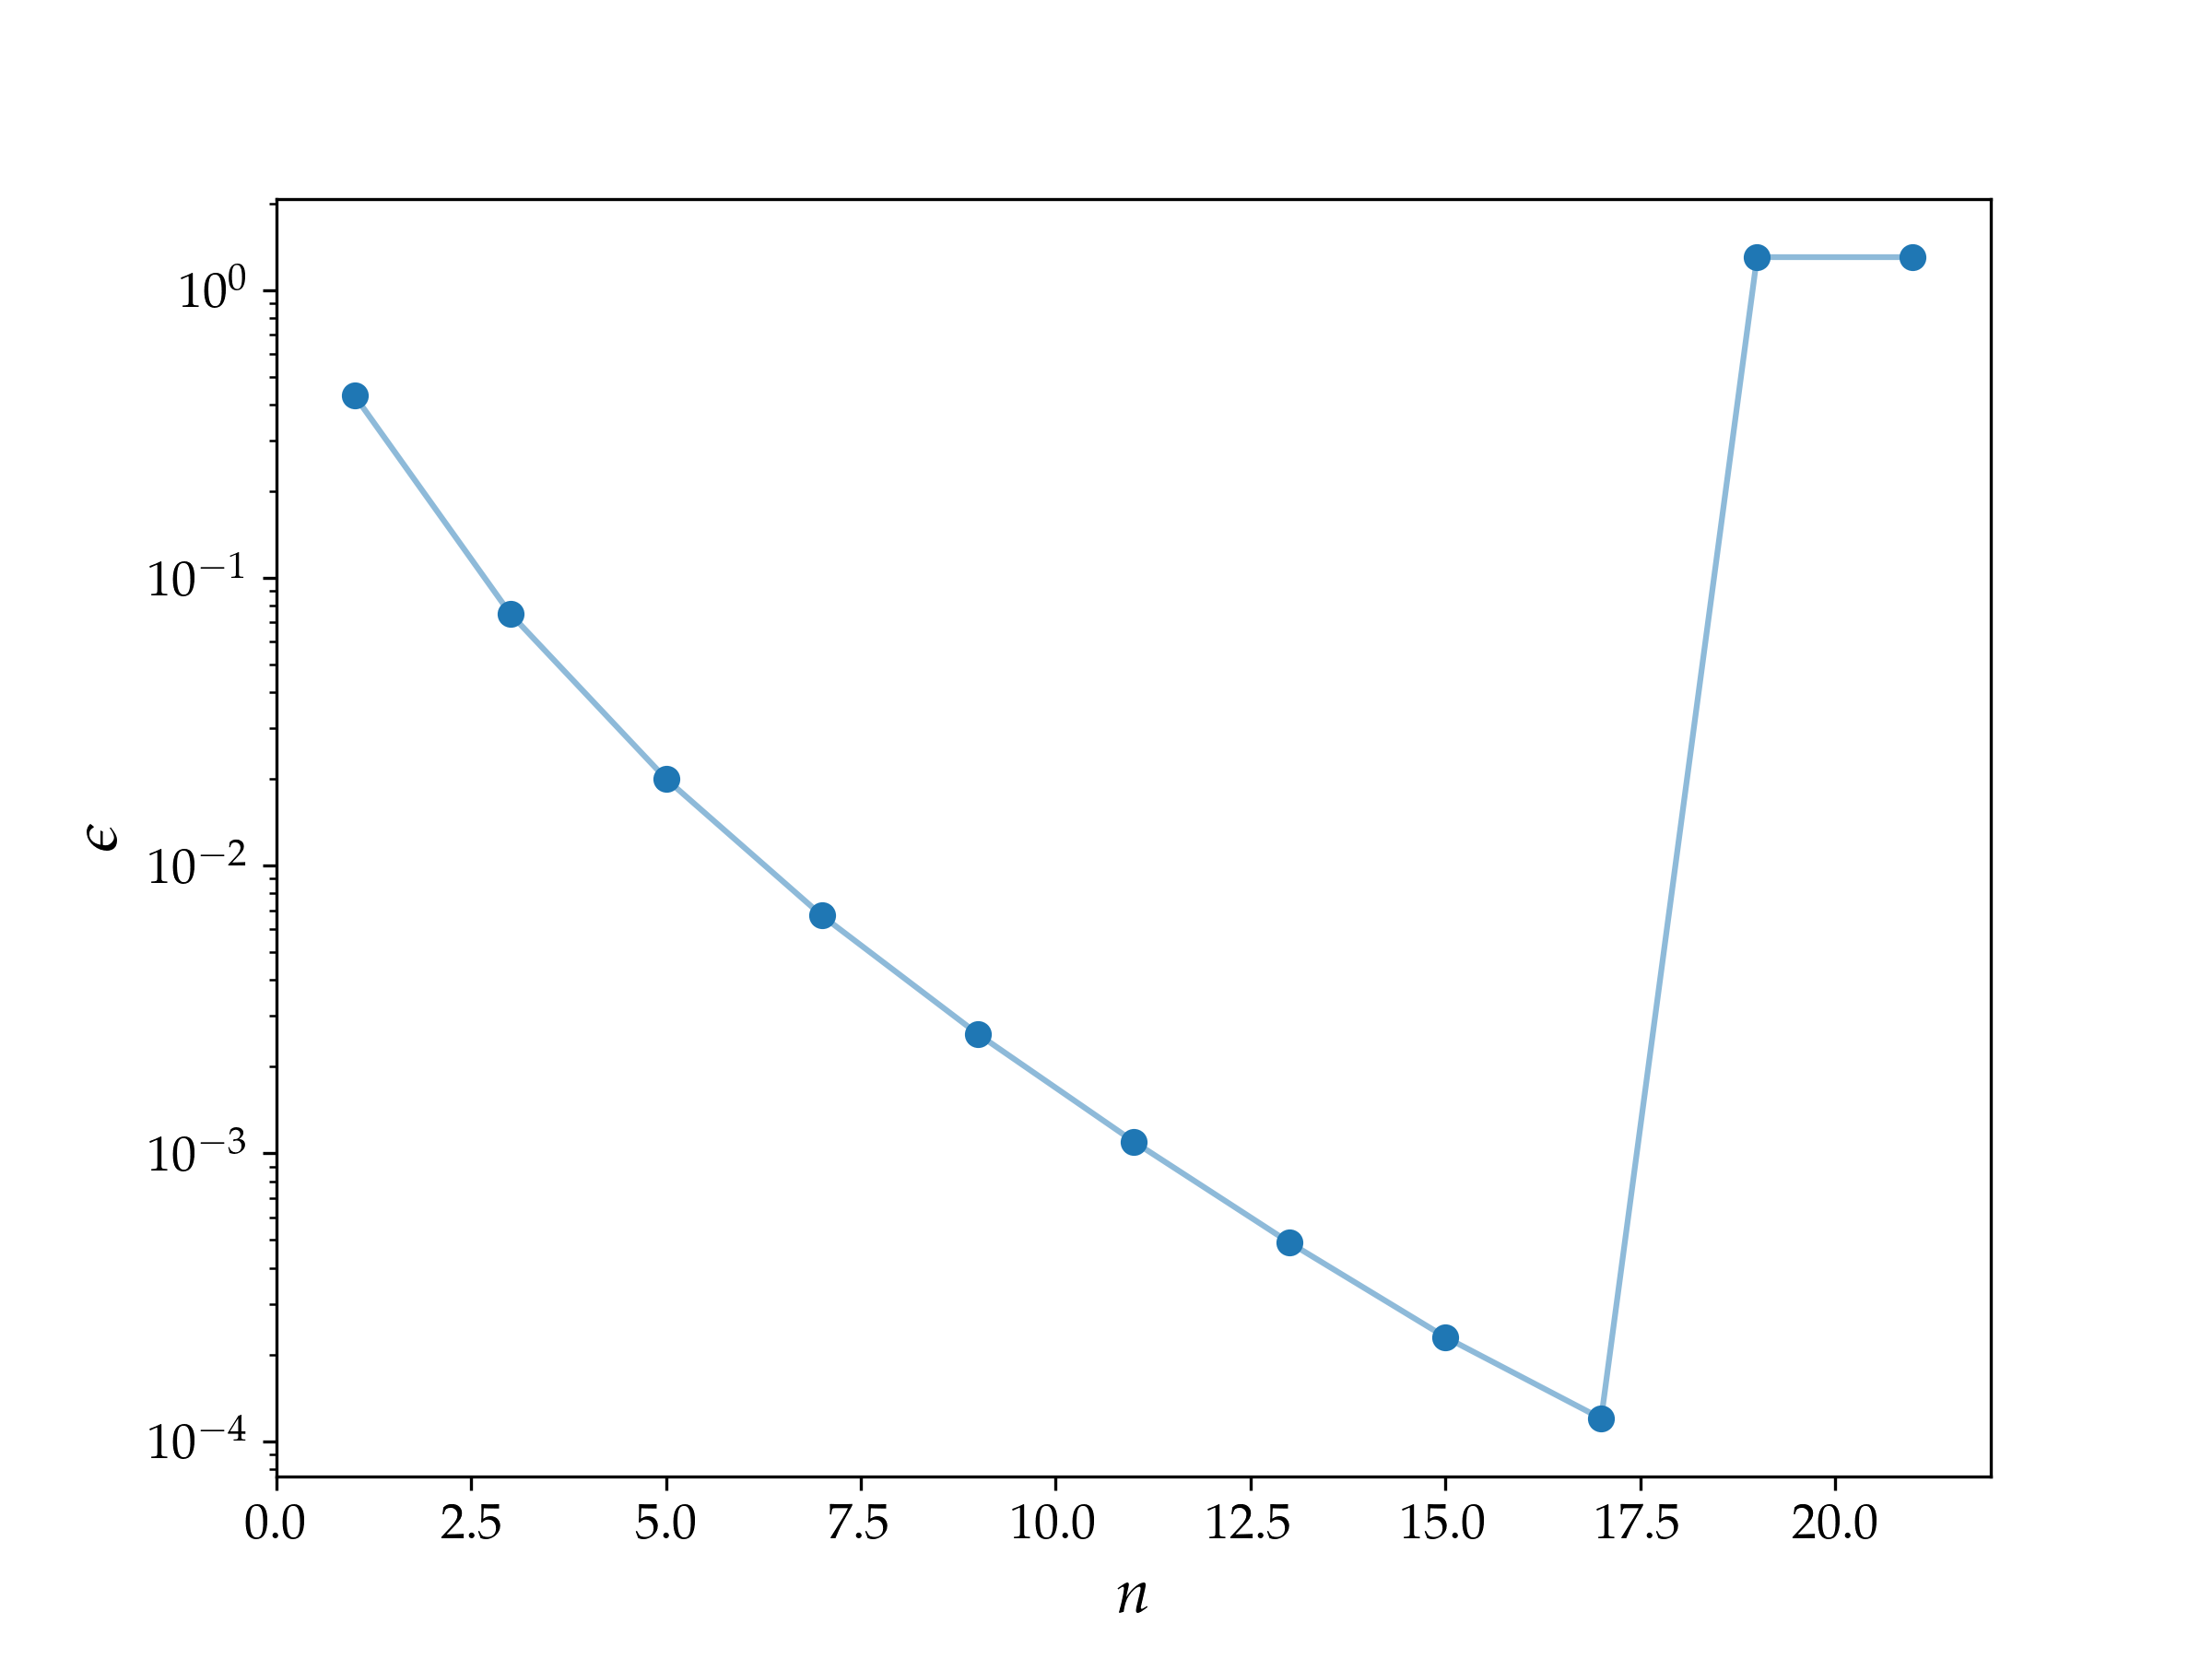
\includegraphics[width=0.7\linewidth]{images/22/int_1.png}
        \caption{Andamento dell'errore per l'integrale $I_1$, in funzione del numero di nodi (radici del polinomio di Hermite).}
        \label{fig: int_1}
    \end{figure}

    \begin{figure}[H]
        \centering
        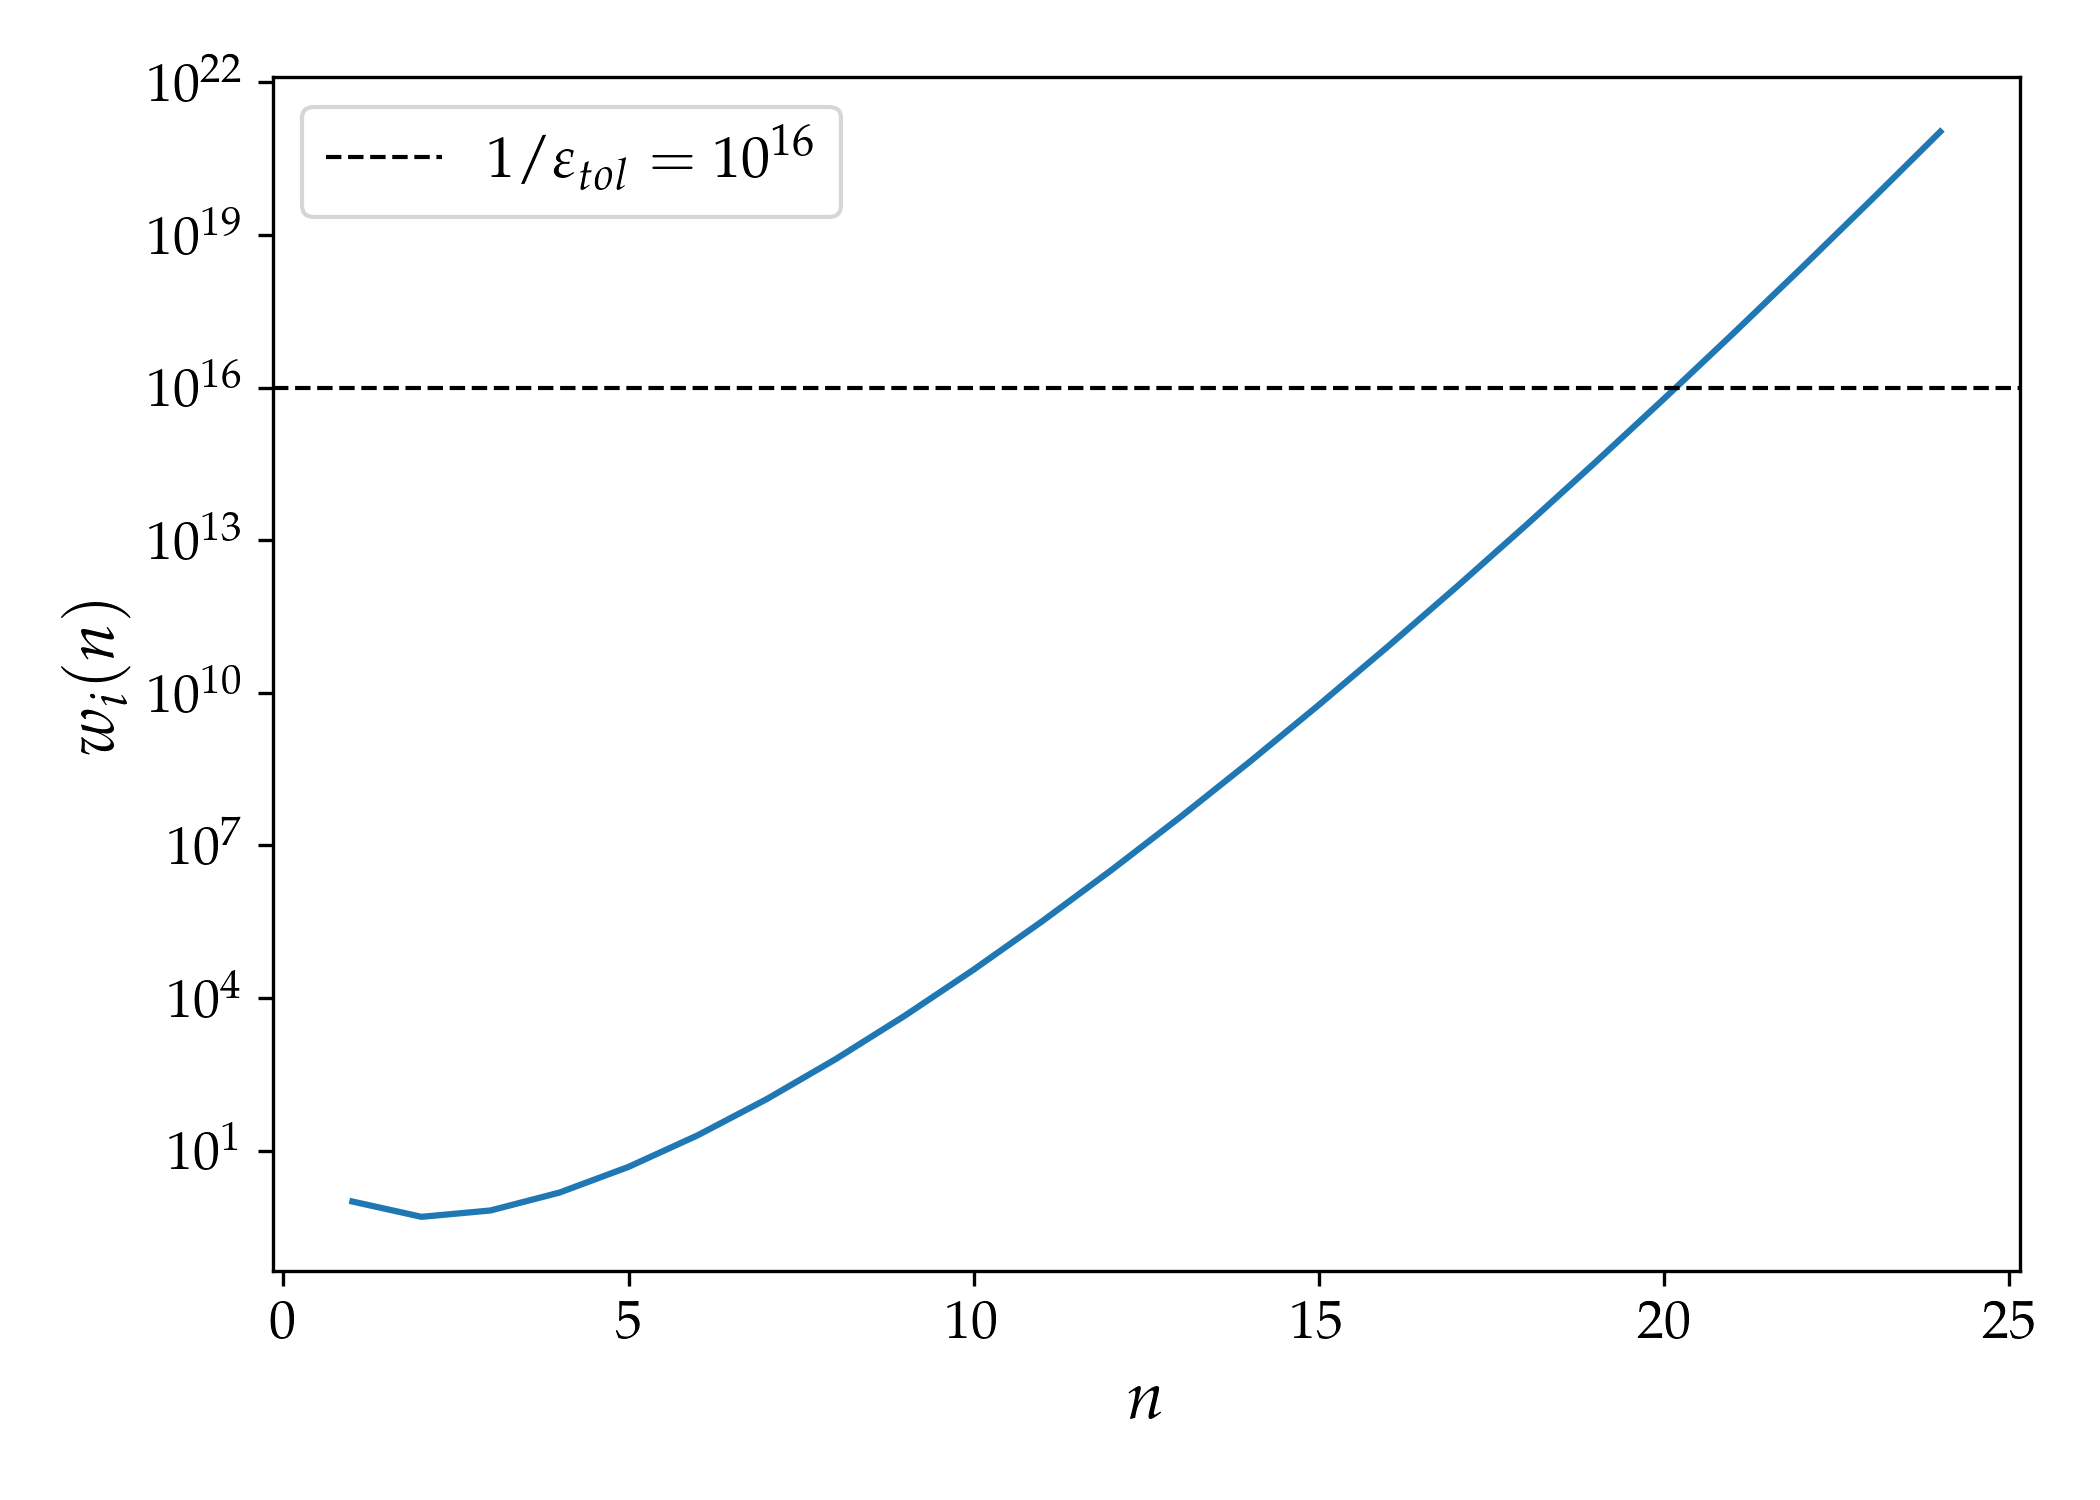
\includegraphics[width=0.7\linewidth]{images/22/asym_weight.png}
        \caption{Andamento asintotico della funzione $w_i$ in funzione di $n$. Nel grafico viene rappresentata $f(n) = \frac{(n-1)!}{n}$}
        \label{fig: asymp_wei}
    \end{figure}

    
    
    
    
    \item $\int_0^\infty dx \, x^{8} \, e^{-x^2} = \frac{105}{32}\sqrt{\pi}\approx 5.82$
    
    \medskip\noindent
    Il caso della seconda funzione ha la caratteristica di non trovarsi in forma esplicita così come ci viene presentata: dobbiamo riportare l'integrale con le condizioni necessarie per l'applicazione del metodo.

    In particolare sapendo che la funzione $h(x) = x^8e^{-x^2}$ è pari, possiamo ridefinire semplicemente sull'intervallo simmetrico come:
    \[
    \int_0^\infty dx \, x^{8} \, e^{-x^2} \to \int_{-\infty}^\infty dx \, \frac{x^{8}}{2} \, e^{-x^2}
    \]

    La funzione $f(x)$ per l'algoritmo diventa quindi:
    \[
    f(x) = \frac{x^{8}}{2} 
    \]

    I risultati numerici di seguito, in Fig. \ref{fig: int_2} lo studio in funzione di $n$.

\begin{elegantcode}
Results of the study:
     TRUE                --> I = 5.815864198283724

     Gauss quadrature    --> I = 5.8158641982835775
                             err = 1.47e-13
\end{elegantcode}

    In particolare si noti come l'errore raggiunga un minimo per un piccolo numero di nodi ($n=7$), poi inizia a crescere per infine attestarsi su un plateau, non convergendo definitivamente a valore vero. La spiegazione è del tutto simile a quella fatta per il caso precedente.  
    
    \begin{figure}[H]
        \centering
        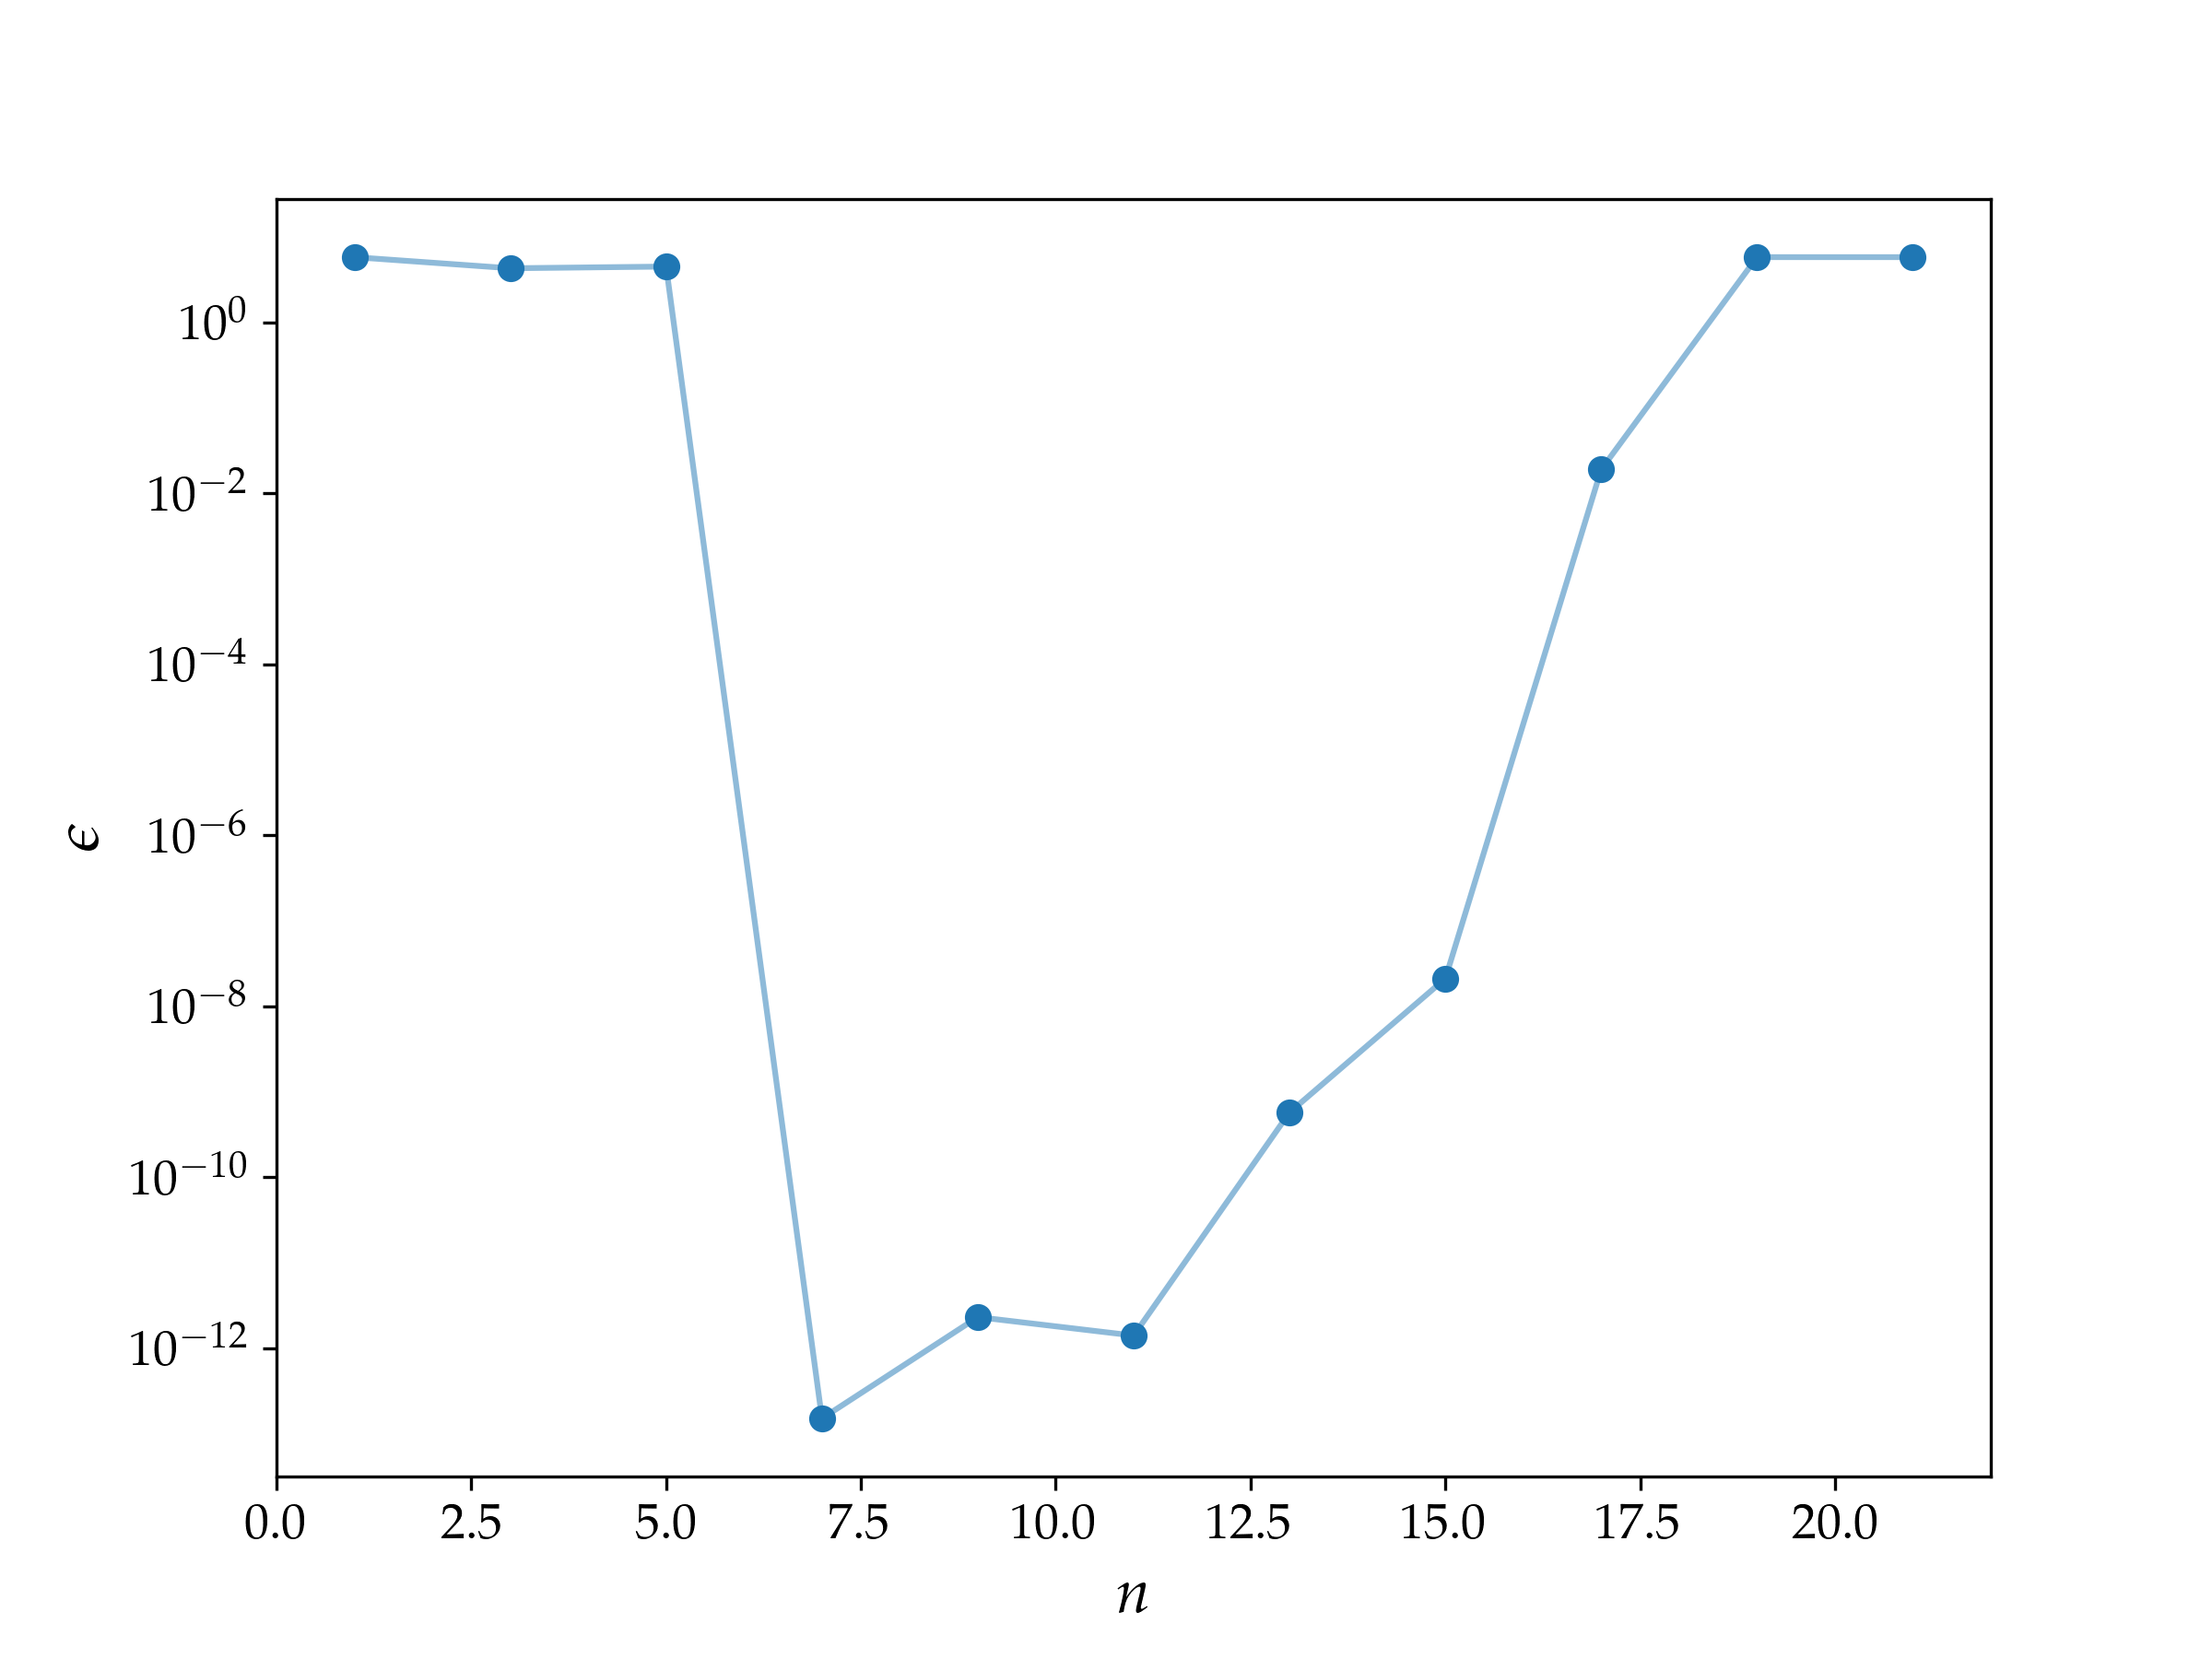
\includegraphics[width=0.7\linewidth]{images/22/int_2.png}
        \caption{Andamento dell'errore per l'integrale $I_2$, in funzione del numero di nodi (radici del polinomio di Hermite).}
        \label{fig: int_2}
    \end{figure}

    
    
    \item $\int_{3}^\infty dx x^5 \, e^{-x^2}=\frac{101}{2}e^{-9}\approx 6.23 \times10^{-3}$
    
    \medskip\noindent
    Infine per questo ultimo caso riportare la funzione nella forma analitica richiesta, non mi è stato possibile. Non ho trovato alcuna caratteristica che potesse permettere un cambio di variabili utile o una simmetrizzazione come nel secondo caso. La mia scelta è stata di definire 
    \[
    f(x) = x^5 H(x-3)
    \]

    dove $H(x-3)$ è la funzione di Heaviside, che vale:
    $H(x) = $
\begin{cases}
1   \quad x\ge3\\
0   \quad x<3
\end{cases}

    così facendo annulliamo manualmente la funzione al di fuori del nostro dominio di interesse, introducendo però una delta di dirac nella derivata (la derivata di $H'(x=3)$ in senso distribuzionale è proprio la $\delta(3)$). La funzione non è più liscia come ipotizzavamo introducendo questo metodo di risoluzione; la discontinuità degrada l'ordine pratico di convergenza e rende la quadratura molto meno efficiente. Potremo osservare come questa scelta introduce un certo grado di oscillabilità nella soluzione numerica, che non potrà competere con la precisione degli altri metodi di integrazione, come sarà possibile notare nei confronti diretti.

    Seguono i risultati dello studio, che è stato ripetuto anche per gli altri metodi numerici, associando al valore di $n$ il significato di numero di intervalli in cui viene suddiviso il $\Delta x$, cioè l'intervallo grande in cui valutiamo la funzione. Gli algoritmi che avevamo già introdotto, quello dei trapezi e di Simpson, possono lavorare direttamente con la formula analitica fornita in prima battuta, a patto di scegliere un intervallo di integrazione finito: se $I=[3, +\infty)$ è l'intervallo originario, imponiamo che i metodi lavorino su $\Tilde{I} = [3, 7]$. 
    
    Si verifica che la funzione è monotona decrescente per $x>3$ e che $f(7)\approx10^{-17}$, cioè al di sotto della nostra \textit{machine precision}. Consideriamo la funzione sulla parte destra di questo intervallo trascurabile per le nostre valutazioni. 
    In Fig. \ref{fig: val_func} si mostra l'intervallo di valutazione che abbiamo appena commentato.

\begin{elegantcode}
Results of the study:
     TRUE                --> I = 6.23e-03

     Gauss quadrature    --> I = 7.43e-03
                             err = 1.19e-03

     Trapezoidal         --> I = 6.62e-03
                             err = 3.90e-04

     Simpson             --> I = 6.24e-03
                             err = 8.82e-06
\end{elegantcode}

    
    \begin{figure}[H]
        \centering
        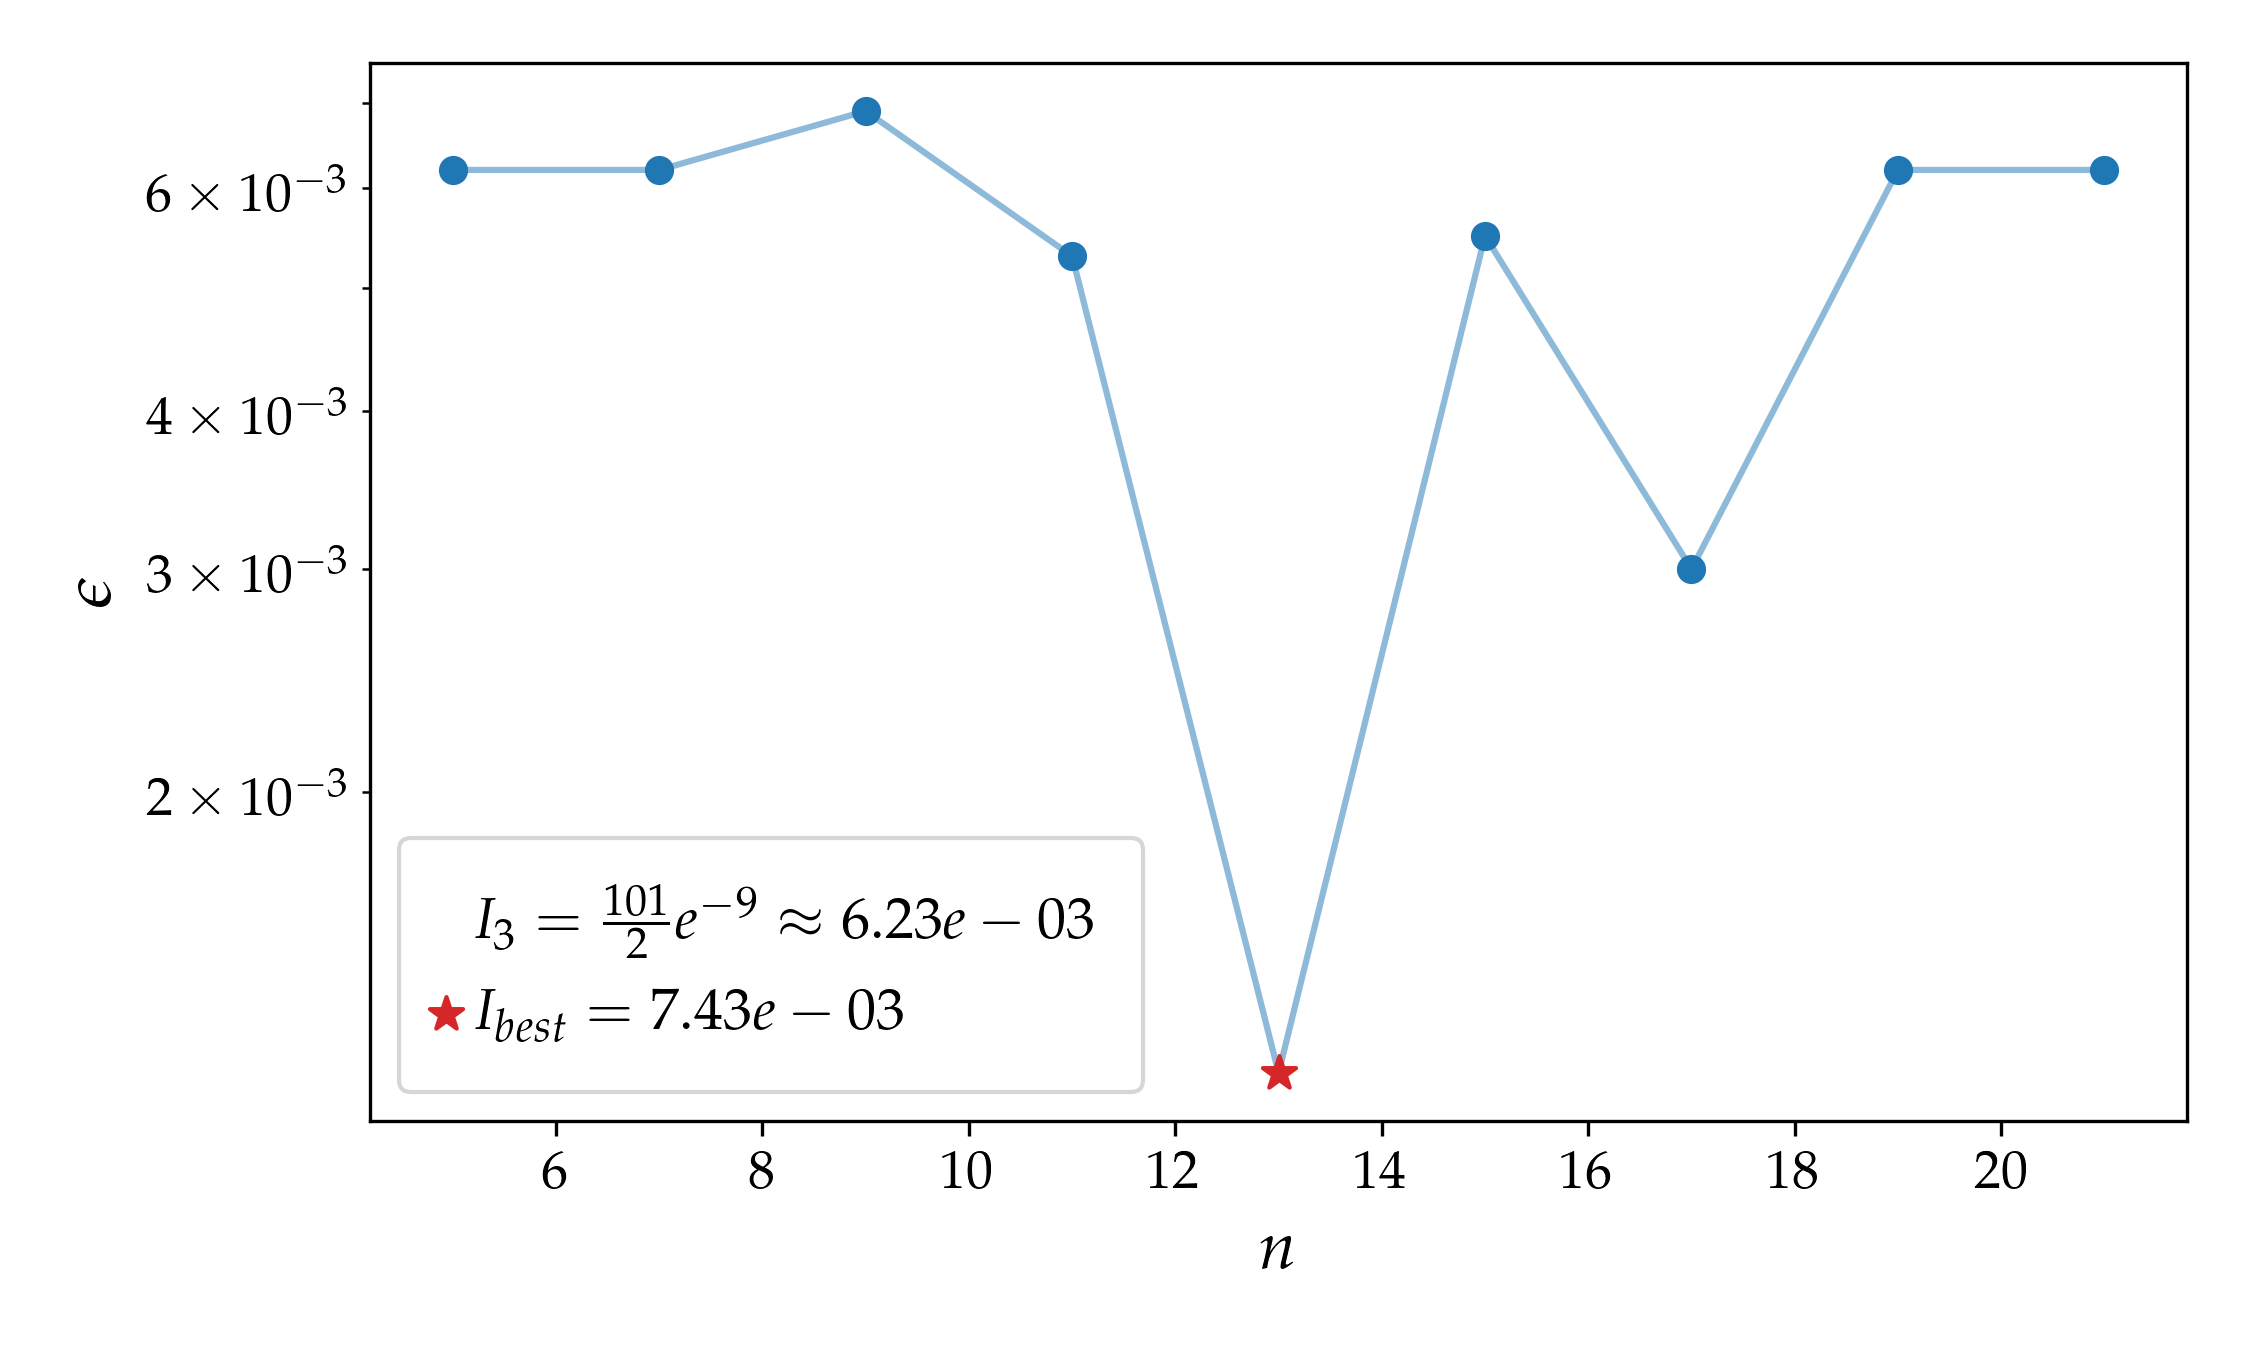
\includegraphics[width=0.7\linewidth]{images/22/int_3.png}
        \caption{Andamento dell'errore per l'integrale $I_3$, in funzione del numero di nodi (radici del polinomio di Hermite).}
        \label{fig: int_3}
    \end{figure}
    
    \begin{figure}[H]
        \centering
        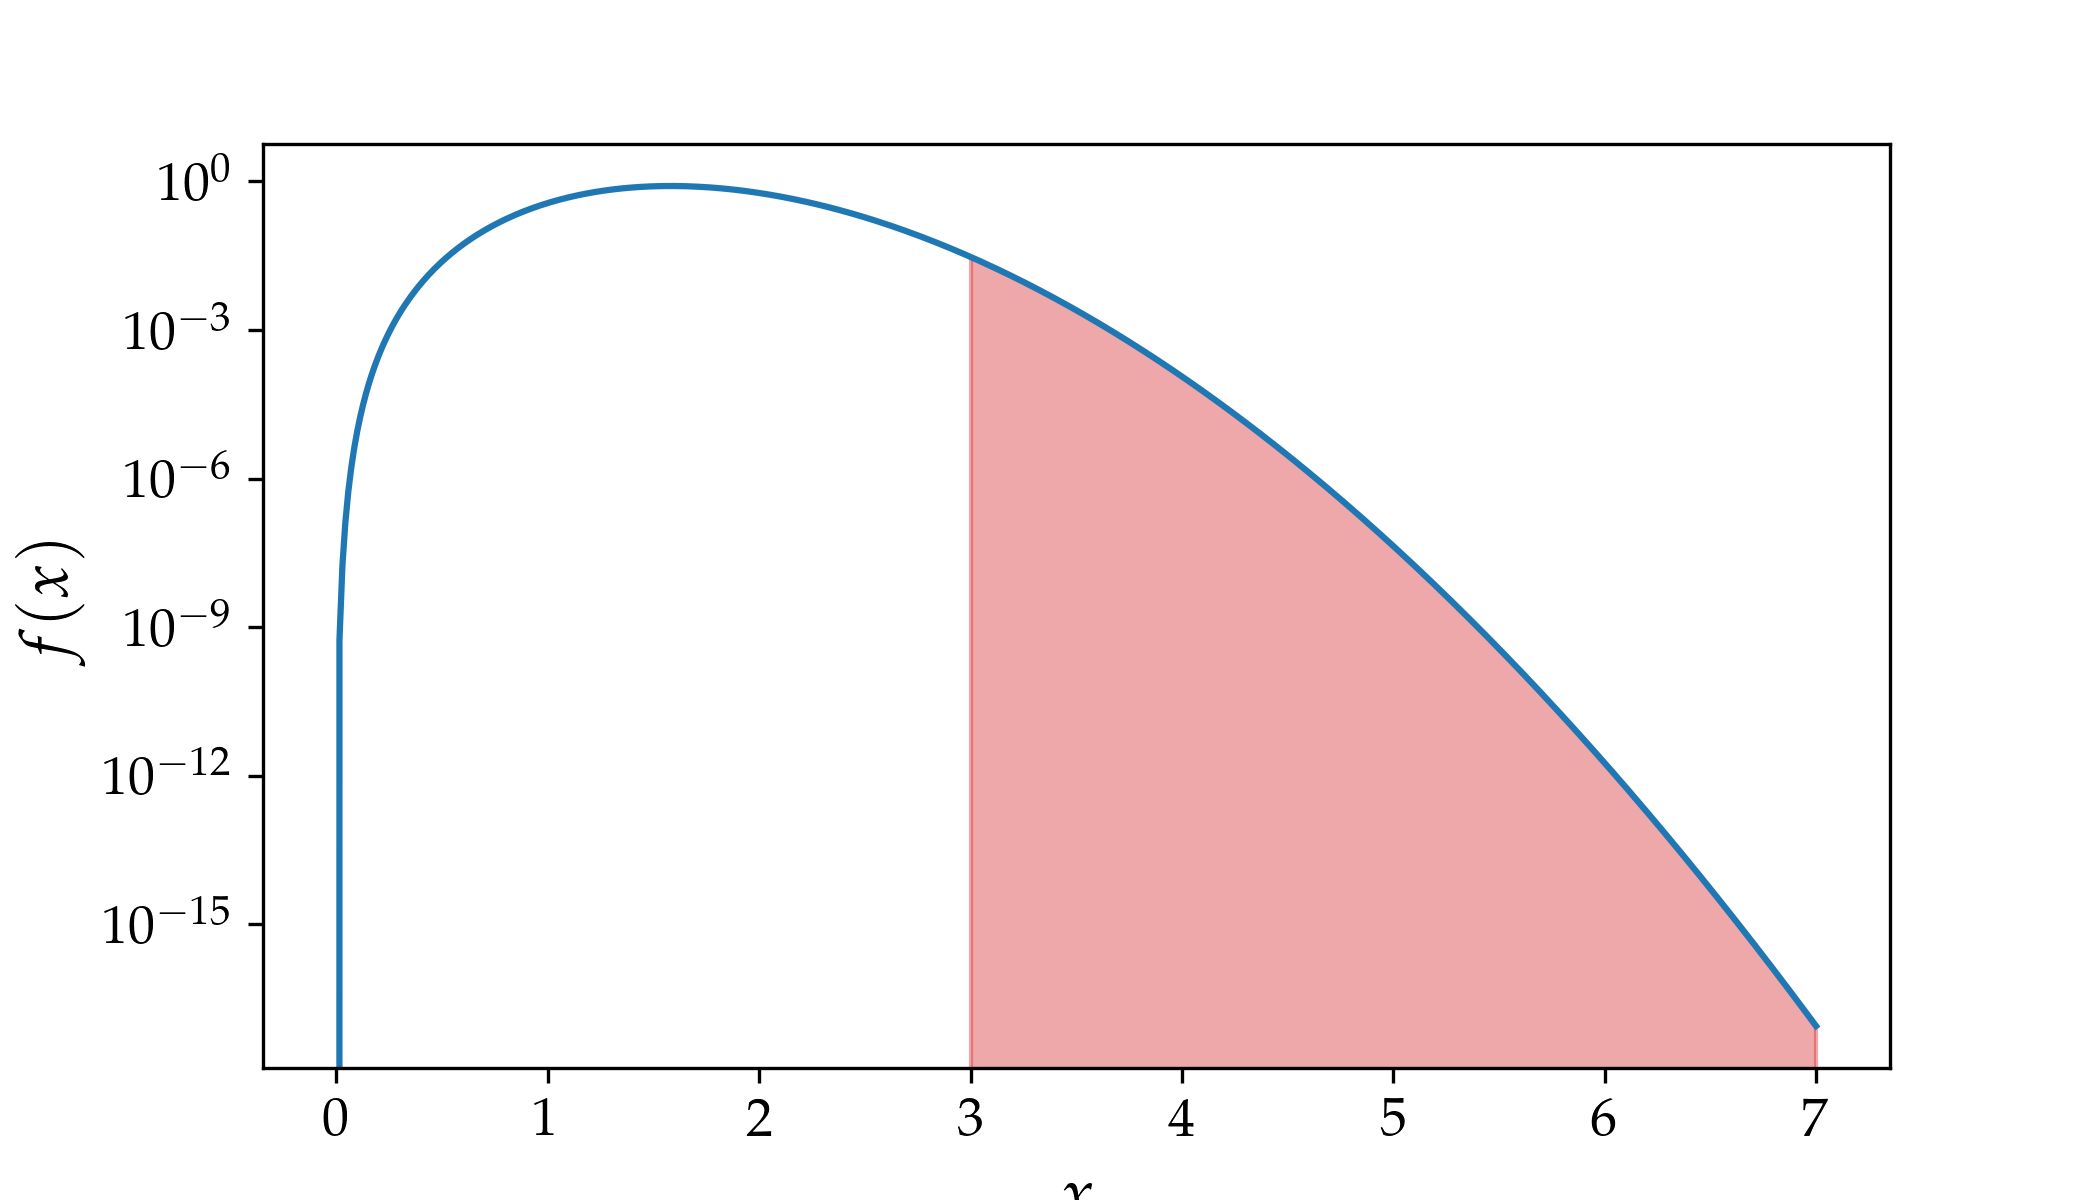
\includegraphics[width=0.7\linewidth]{images/22/func_display_part.png}
        \caption{Intervallo di valutazione della funzione.}
        \label{fig: val_func}
    \end{figure}

    In particolare si noti come il metodo risulti instabile e poco accurato: l'errore non riesce a scendere sotto l'ordine di $10^{-3}$ neanche nel punto in cui otteniamo il miglior risultato. Una figura che è ancora più esplicativa è quella relativa al confronto della convergenza dei metodi, Fig. \ref{fig: conv_mth}. Si noti la convergenza asintotica di Simpson e dei trapezi, mentre l'algoritmo della quadratura di Gauss-Hermite non è convergente, ha invece carattere oscillatorio.

    \begin{figure}[H]
        \centering
        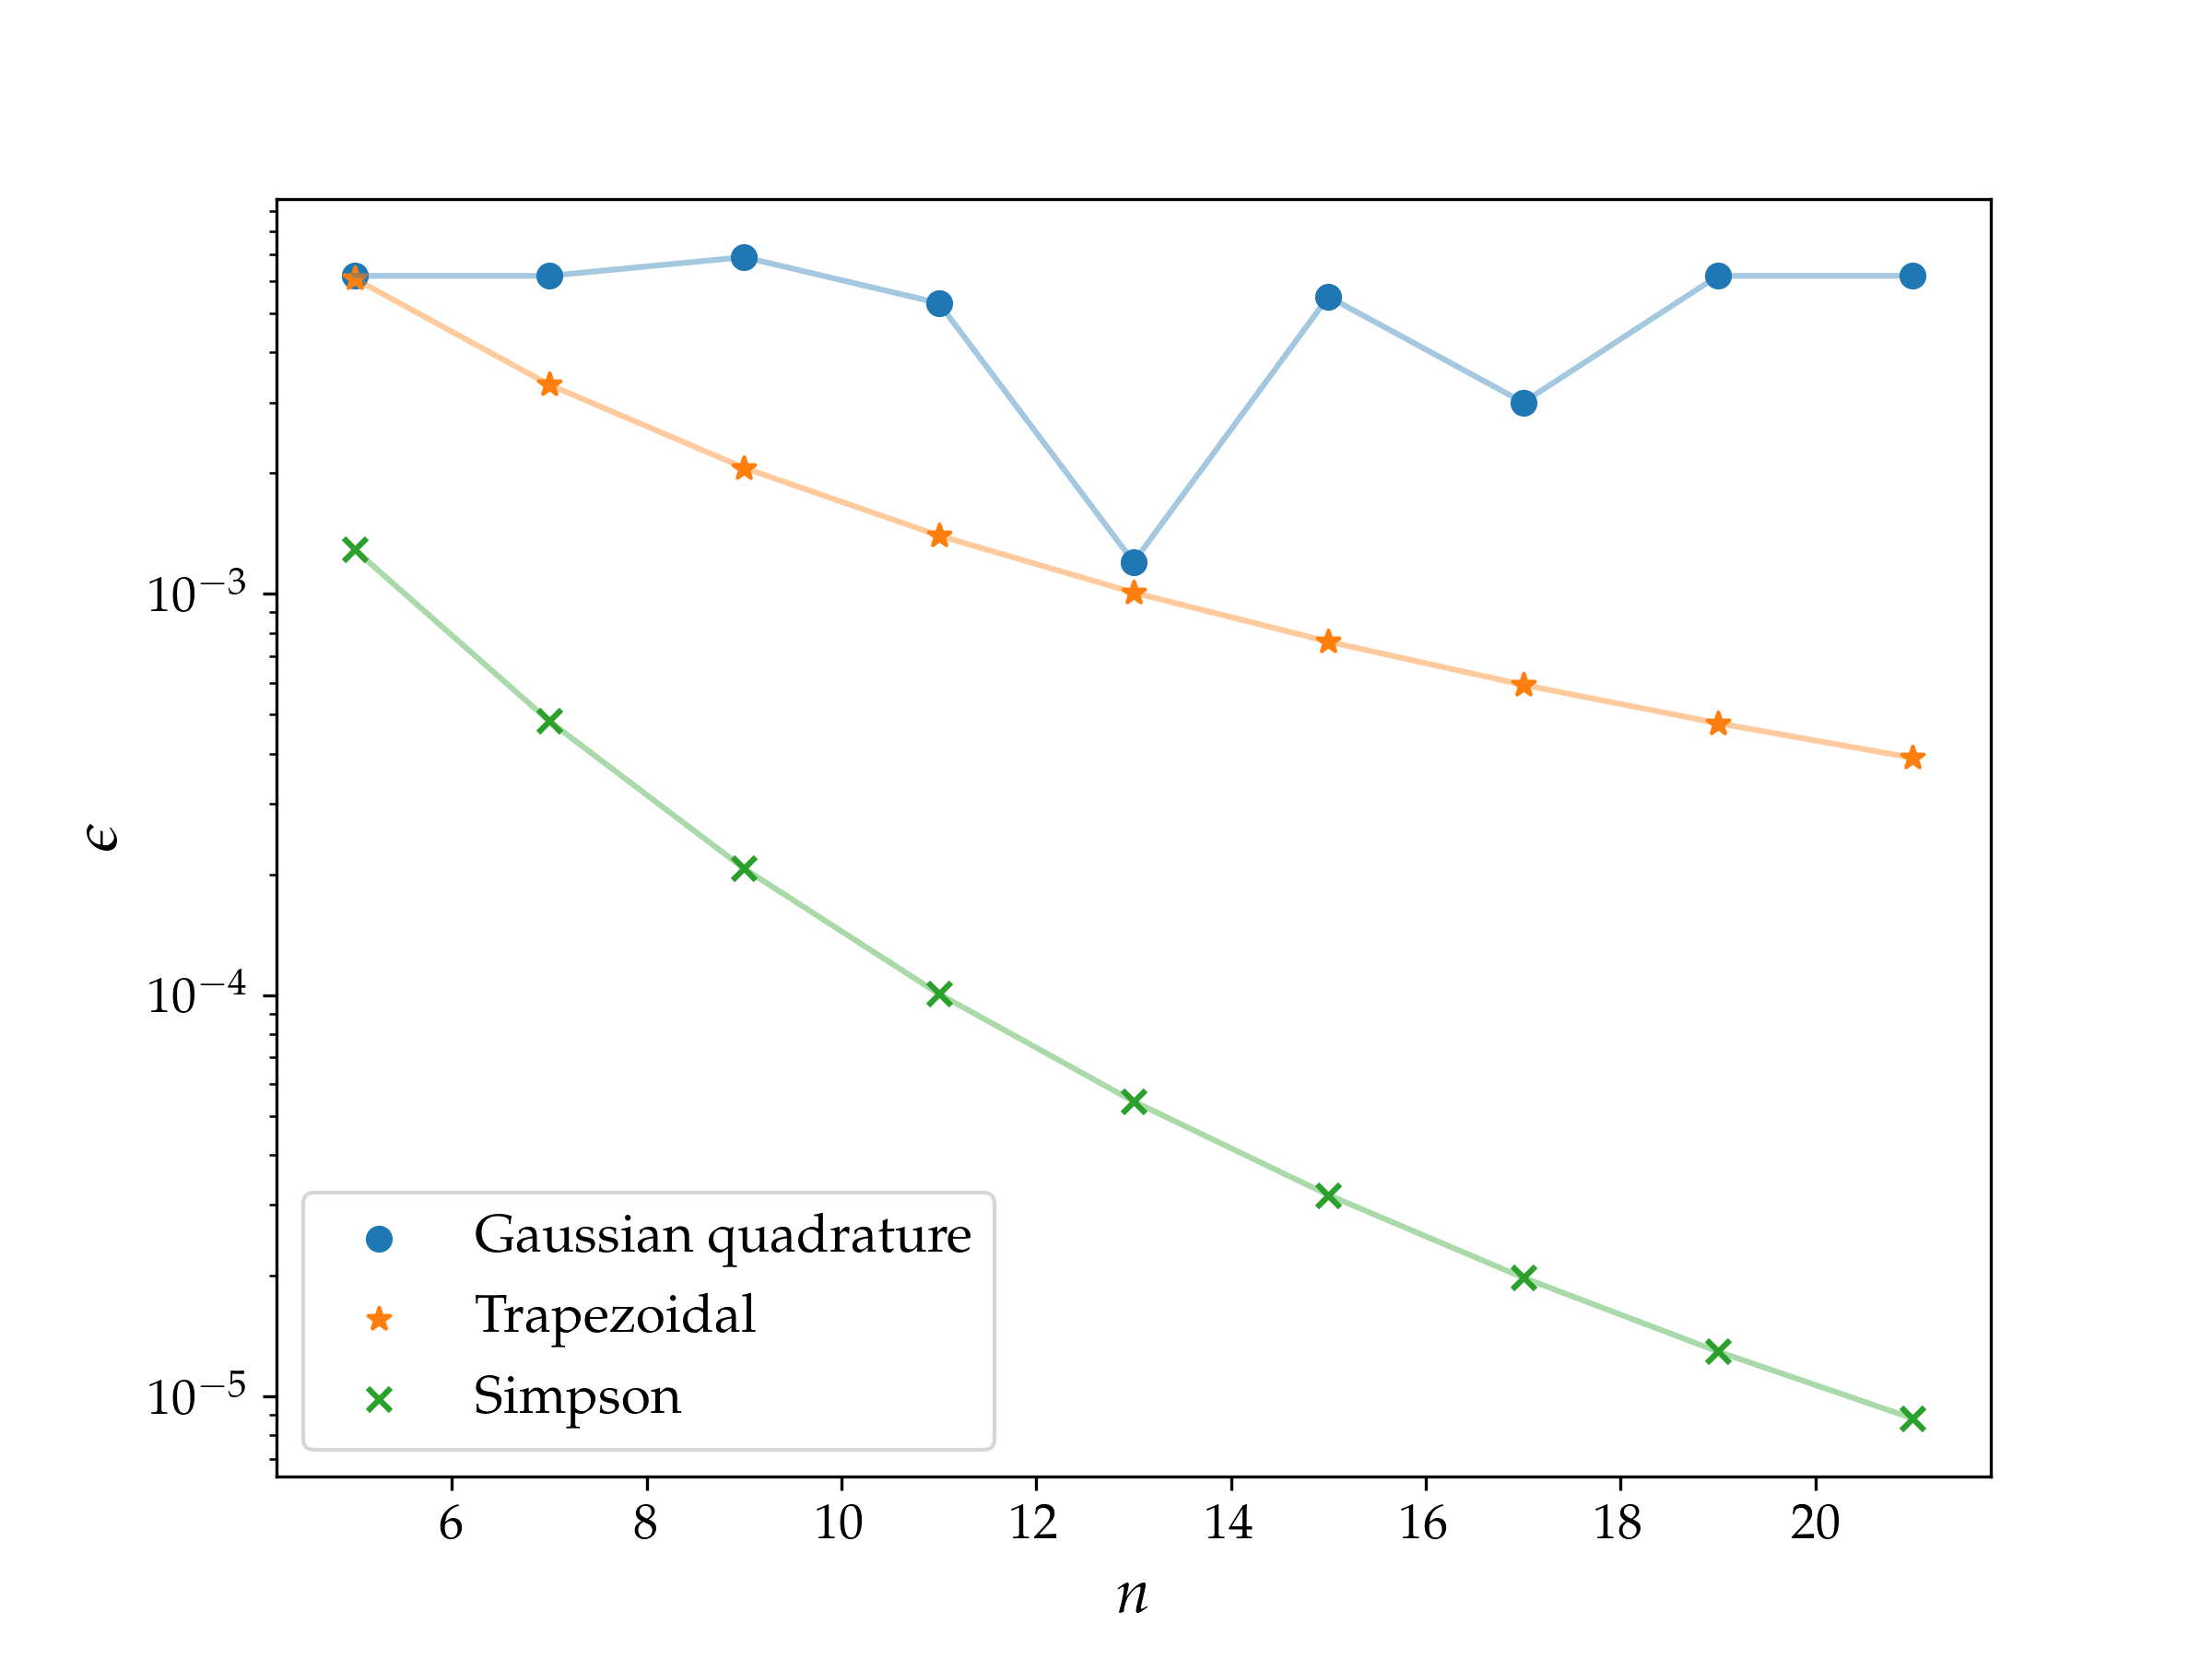
\includegraphics[width=0.7\linewidth]{images/22/confr.png}
        \caption{Confronto diretto dei tre metodi numerici per la valutazione dell'integrale $I_3$.}
        \label{fig: conv_mth}
    \end{figure}

    È anche possibile confermare l'andamento dei due metodi per precisioni maggiori, scegliendo $n$ più grandi, che invece bloccherebbero l'esecuzione del primo algoritmo. Osserviamo in Fig. \ref{fig: conv_mth_fit} come la pendenza rispecchia ciò che ci aspettiamo analiticamente, cioè una convergenza quadratica e quartica rispettivamente per la regola dei trapezi e di Simpson. 

    Si noti che nei grafici è riportata, per continuità con i confronti precedenti, la convergenza in funzione del numero di sottointervalli in cui suddividiamo il dominio. La convergenza è $O(n^p),\ p >0$ quando la osserviamo in relazione allo spacing $\delta x$, il quale è inversamente proporzionale al numero di intervalli; così spiegati gli andamenti asintotici con potenze negative.

    \begin{figure}[H]
        \centering
        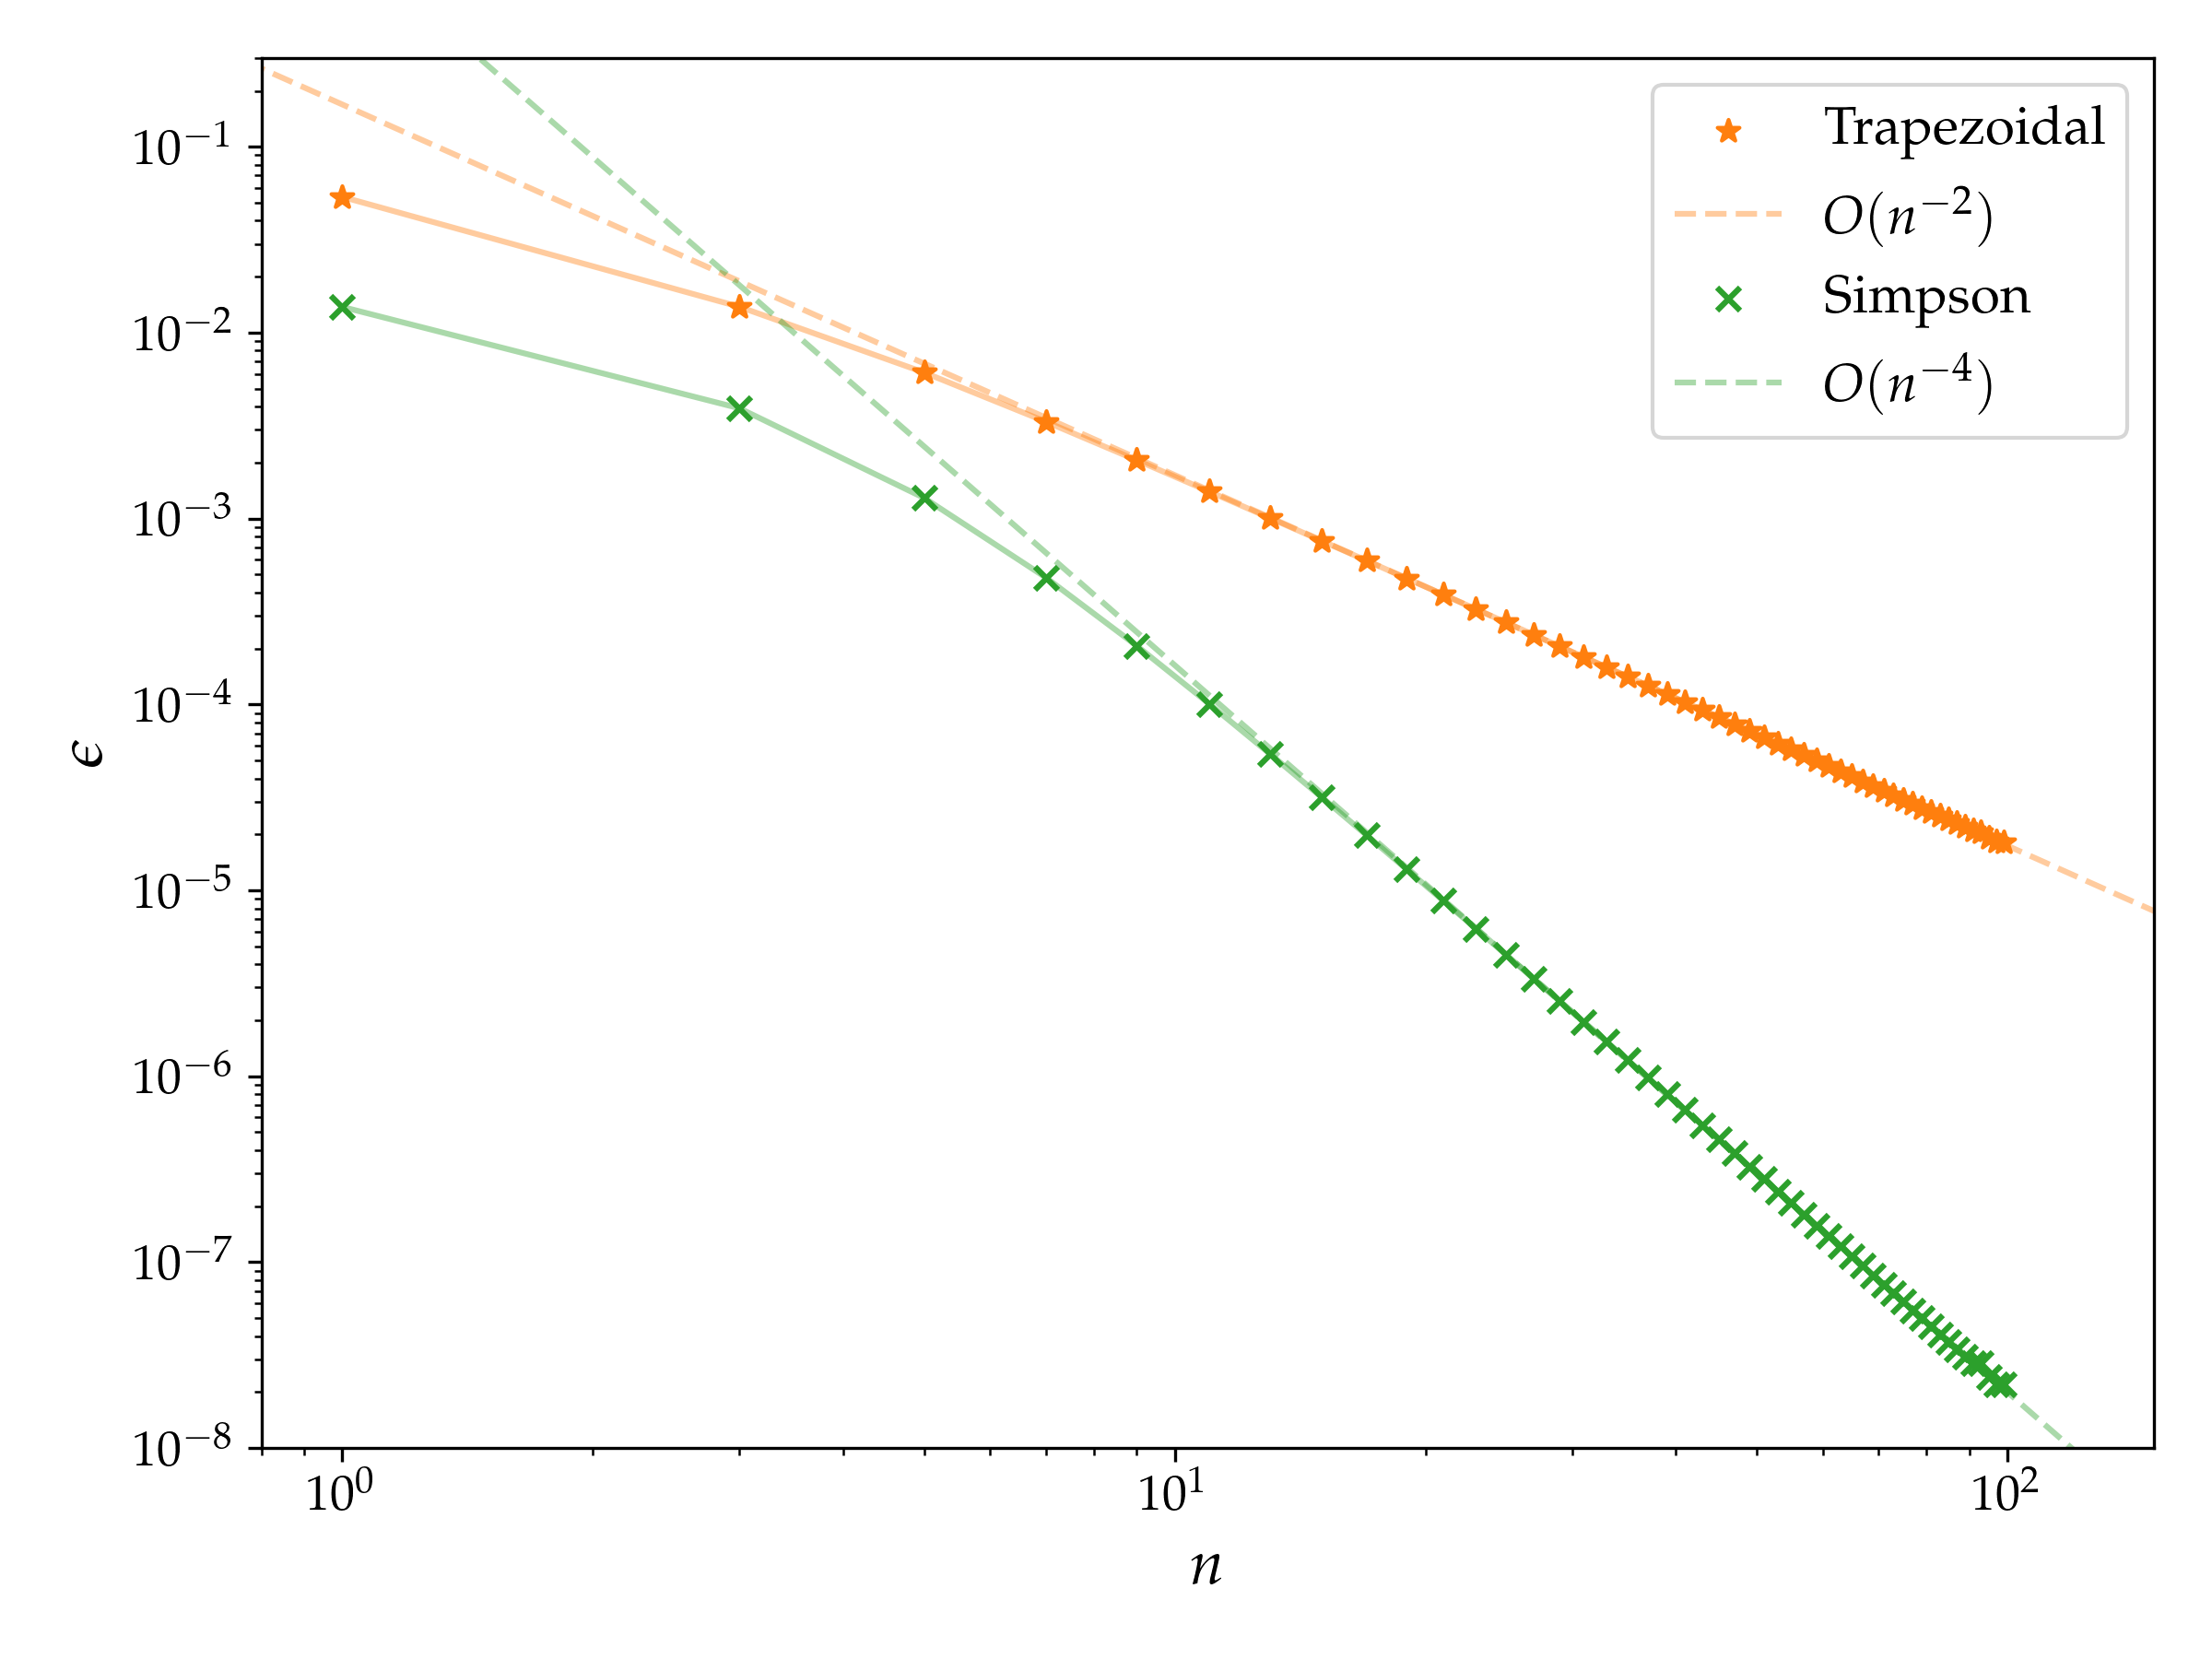
\includegraphics[width=0.7\linewidth]{images/22/confr_fit.png}
        \caption{Confronto della convergenza asintotica per i metodi dei trapezi e di Simpson per $I_3$.}
        \label{fig: conv_mth_fit}
    \end{figure}

        
\end{enumerate}

\bigskip\noindent
Infine si commenta il plot richiesto di $w_i(x_i)$: l'idea di introdurre dei pesi si riferisce alla possibilità di attribuire una importanza diversa a diversi punti di valutazione della funzione, in corrispondenza proprio dei nodi $x_i$, in funzione all'informazione che essi veicolano per calcolare il valore della funzione generale. I pesi quantificano il contributo numerico associato a ciascun nodo della quadratura e la loro distribuzione è una conseguenza delle proprietà di ortogonalità dei polinomi di Hermite.


\begin{figure}[H]
    \centering
    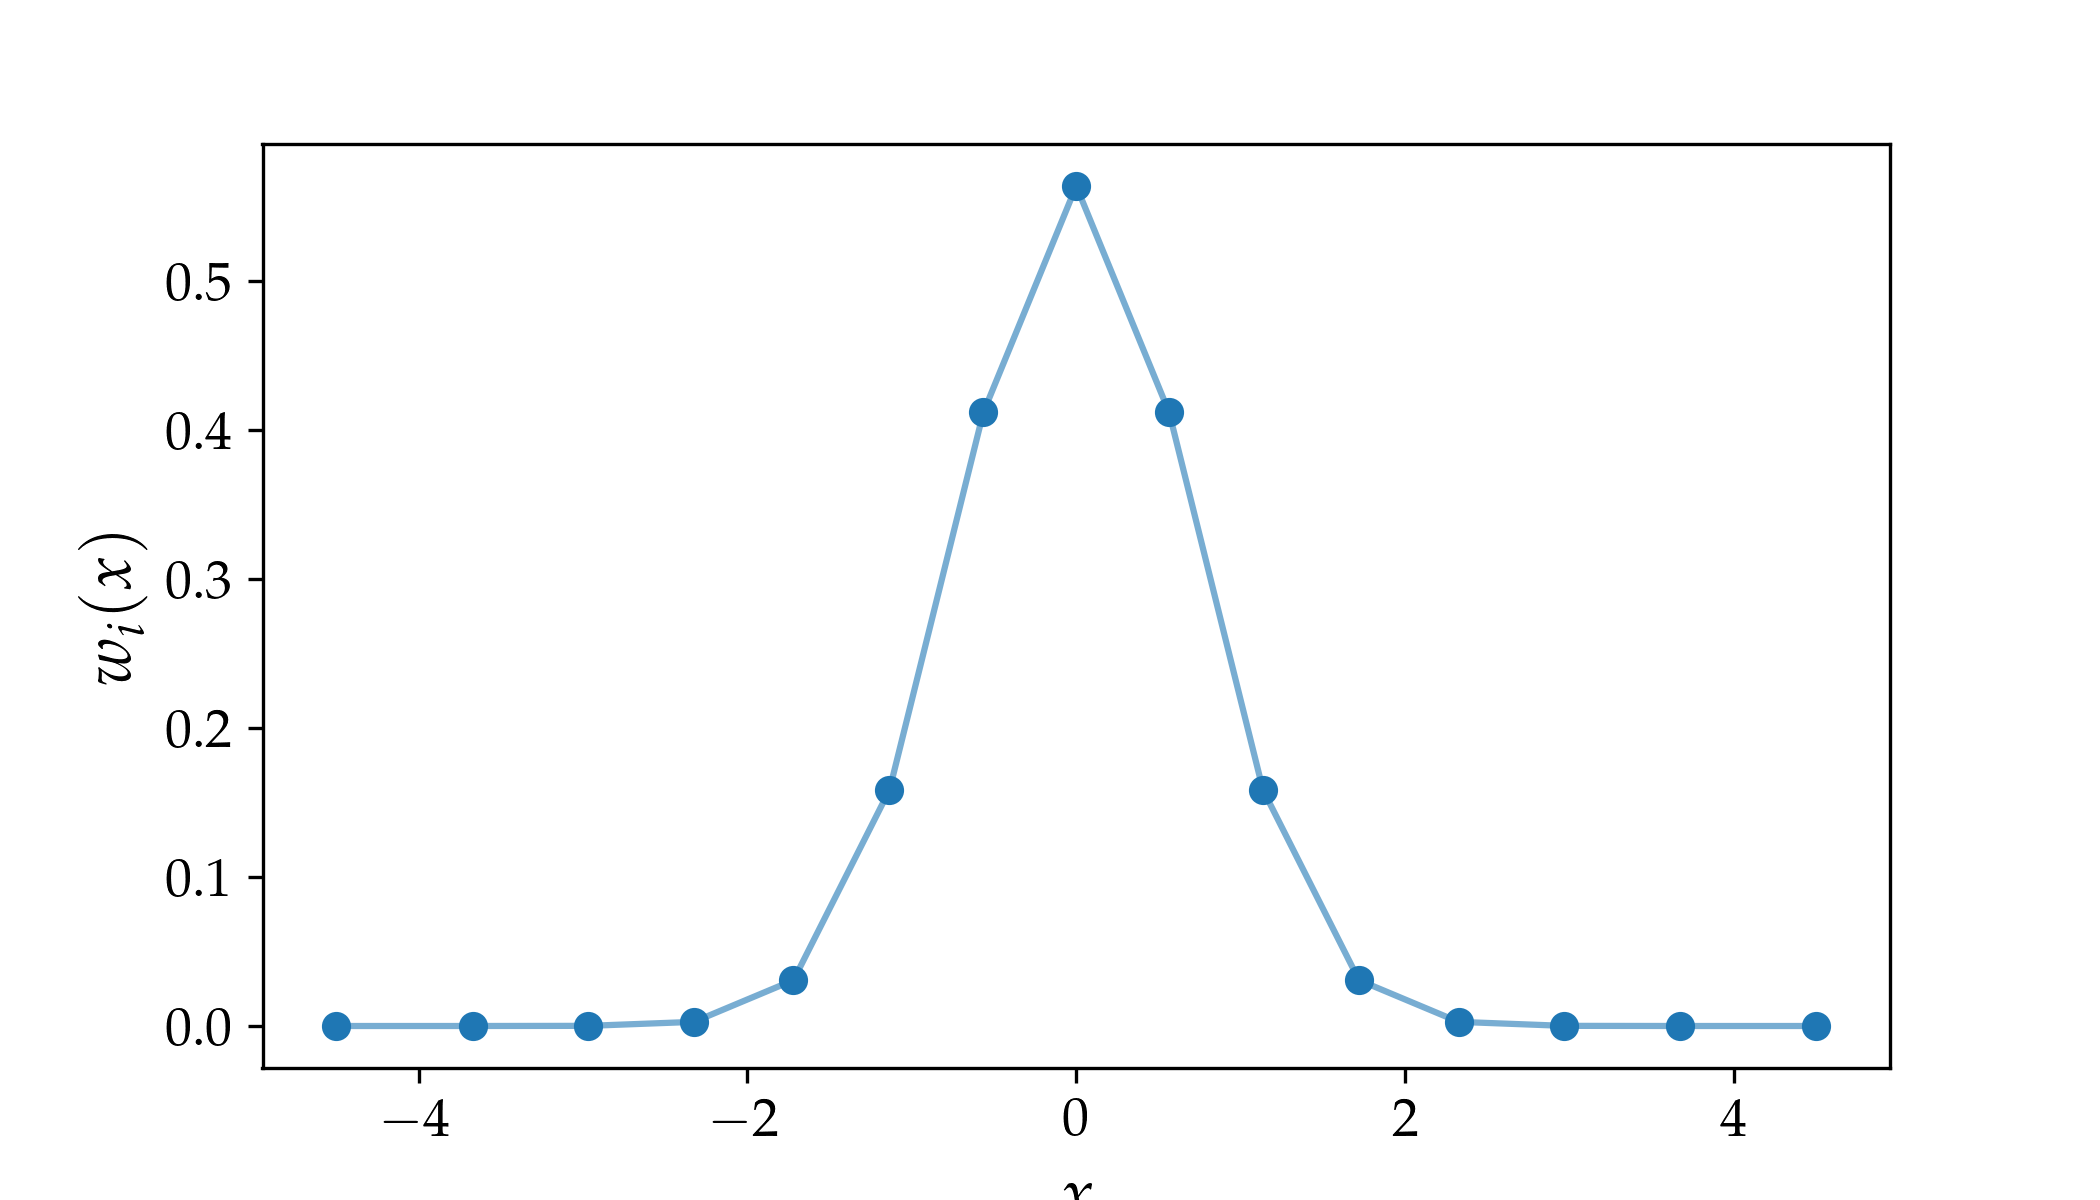
\includegraphics[width=0.7\linewidth]{images/22/weight_example.png}
    \caption{Rappresentazione dei pesi sulle i-esime radici dei polinomi di Hermite.}
    \label{fig: weight_her}
\end{figure}

\newpage












% --------------------------------------------------
% INDENTAZIONE CAPITOLI
% --------------------------------------------------
% --------------------------------------------------
% \cleardoublepage 
% \addtocontents{toc}{\bigskip\noindent\protect\textbf{\Large LOREM IPSUM}\par\smallskip}
% \addtocontents{toc}{\protect\setcounter{tocdepth}{-2}} 
% \part{\Huge LOREM IPSUM}
% \addtocontents{toc}{\protect\setcounter{tocdepth}{2}} 
% --------------------------------------------------

% \section{Esercizio XXX}
% \subsection{Problem Statement}
% \subsection{Premessa Teorica}
% \subsection{Metodi Numerici e Algoritmi}
% \subsection{Risultati e Discussione}
% \newpage


% \section{Conclusioni}
% % Sintesi dei risultati ottenuti.



% --- Appendice ---

\newpage
% \thispagestyle{empty} 
\null 
\clearpage
\newpage
% \thispagestyle{empty} 
\null 
\clearpage




\addtocontents{toc}{\bigskip\bigskip\bigskip\noindent\protect\textbf{\Large Appendice}\par\smallskip}
\addtocontents{toc}{\protect\setcounter{tocdepth}{-2}} 

\part*{\Huge Appendice}
\addtocontents{toc}{\protect\setcounter{tocdepth}{2}} 


\section*{Funzione per fit e esempi d'uso}
\addcontentsline{toc}{section}{Funzione per fit e esempi d'uso}
\label{App: funzione fit}

Uno degli argomenti che abbiamo trattato nel corso è proprio quello del fitting lineare di un sample con una data funzione: questo è stato ben discusso in particolare nel Cap. \ref{Cap: fitting}.\\
È stato naturale costruire una funzione ben articolata che potesse essere di rapido uso in caso di necessità (\lstinline|lib_fitting.py --> lin_fit()|). Essa si articola in due parti principali:


\begin{enumerate}
    \item un oggetto che, tramite minimizzazione ai minimi quadrati (\textit{Least Squares}, LS), determini la curva che meglio interpola i punti, data la relativa matrice di covarianza.
    \item un motore che implementi la rappresentazione grafica, personalizzabile nelle diverse funzionalità, del sample, della curva fittata e eventualmente di altri oggetti grafici.
\end{enumerate}

I dettagli sul codice e sulle specifiche grafiche sono disponibili, eventualmente commentati, nella mia libreria, ci tenevo però a fare una piccola digressione che diventa importante per il reiterato uso che ne farò nel corso del report.
\bigskip

\noindent Spesso accade che sia richiesto confermare o ricercare, per via numerica, quale sia il \textit{rate} di convergenza per determinati algoritmi, questa stima è cruciale per valutarne l'efficienza. Per un metodo con convergenza polinomiale, l'errore $e_n$ al passo $n$ segue la relazione:
\[
    e_n \approx C \cdot n^{-p} \implies \log(e_n) \approx \log(C) - p \log(n)
\]
dove C è una costante e $p$ rappresenta l’ordine di convergenza del metodo. Operativamente, $p$ può essere stimato tramite la pendenza del grafico log-log dell'errore rispetto al numero di iterazioni:
\[
    p \approx -\frac{\log(e_{n+1} / e_n)}{\log((n+1) / n)}
\]
Questa stima è valida nel regime asintotico, dove l'andamento dell'errore si stabilizza su una retta di pendenza $-p$.

\bigskip
\noindent
In questo caso l'utilizzo di una funzione di fitting è naturale: lavoreremo scegliendo 
$$(x, y) \rightarrow (\log(n), \log(e_n))$$ tipicamente riferendoci al $\log_{10}$, per riportare agli ordini di grandezza con cui ci confrontiamo solitamente. 
\noindent Questa formulazione comprende diversi casi di interesse:
\begin{itemize}
\item ($p = 1$): convergenza lineare;
\item ($1 > p > 2$): convergenza superlineare;
\item ($p = 2$): convergenza quadratica.
\end{itemize}

\bigskip
\noindent
Un ulteriore esempio è nello studio numerico della convergenza degli algoritmi iterativi. In molti casi, infatti, l’errore al passo successivo può essere espresso asintoticamente come funzione di quello corrente:
\[
e_{k+1} \approx C \cdot e_k^{p}
\]
Applicando il logaritmo alla relazione precedente si ottiene:
\[
\log(e_{k+1}) \approx \log(C) + p\log(e_k)
\]

\noindent L'analisi che se ne può fare è del tutto simile a quella discussa per il caso precedente.

\bigskip
\noindent
Per mantenere la generalità dell'uso della funzione sarà necessario fornire anche la matrice di covarianza: viene scelta la matrice identità quando stiamo facendo questo tipo di analisi, poiché equivale ad assegnare lo stesso peso a tutti i punti, in assenza di una stima statistica affidabile delle incertezze. La conseguenza di ciò è che i valori presentati in output, come $\chi^2$, il \textit{p-value} o le incertezze sui valori attesi, non hanno significato statistico e sono quindi da non considerare. Sarà importante tenere di conto questo per eventuali valutazioni sui risultati delle operazioni. 

\newpage



\section*{Evoluzione temporale nell'equazione di Schröedinger}
\addcontentsline{toc}{section}{Evoluzione temporale nell'equazione di Schröedinger}
\label{App: rappr schr}

Le animazioni sono sicuramente la scelta più completa per la rappresentazione di una evoluzione temporale, poiché mostrano in maniera comprensibile e intuitiva come si modificano alcune caratteristiche del sistema.
A differenza dei plot statici (in cui attivamente abbiamo scelto di non rinormalizzare ogni figura per esaltare le forme di interferenza), qui la normalizzazione è assicurata in ogni istante, a meno di oscillazioni numeriche, dal funzionamento di RK4 (a differenza del metodo di Eulero che si dimostra non conservare la norma).

\medskip\noindent
Ho scelto di mostrare nelle immagini anche il potenziale, che viene plottato in sovraimpressione con trasparenza al $50\%$. Qui sotto un confronto di un plot con o senza: la scelta è per privilegiare un grafico più manifesto e completo (nella repo Github è possibile ottenere anche i grafici in cui è stato omesso questo particolare, ed è possibile riprodurli con il codice lavorando su dei semplici switch che ho inserito nella prima parte del programma, \url{https://github.com/mvolpato-unimib/Lab_comp/tree/main/ex19/st_plots}).

\begin{figure}[H]
    \centering
    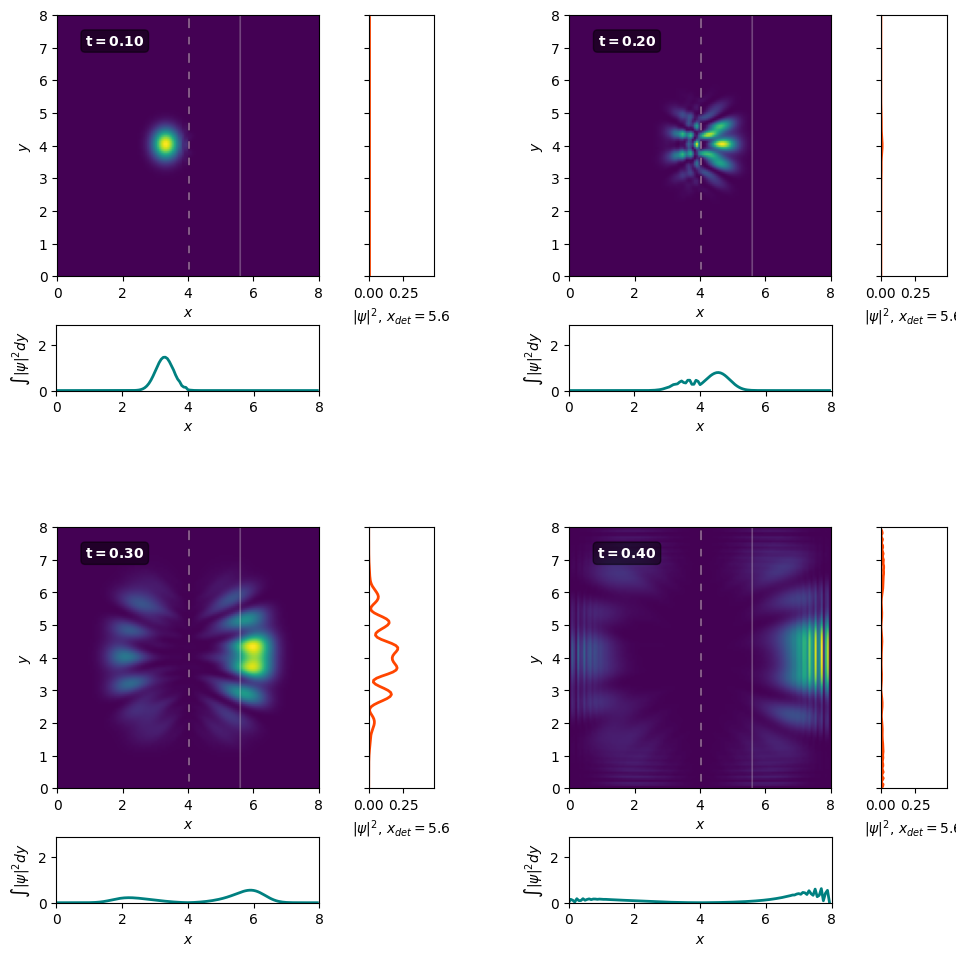
\includegraphics[width=0.7\linewidth]{images/19/pot/diff_grate_pot.png}
    \caption{Reticolo di diffrazione, rappresentazione con il potenziale statico $V(x, y, t)$ visibile in sovraimpressione.}
    \label{fig:placeholder}
\end{figure}

\begin{figure}[H]
    \centering
    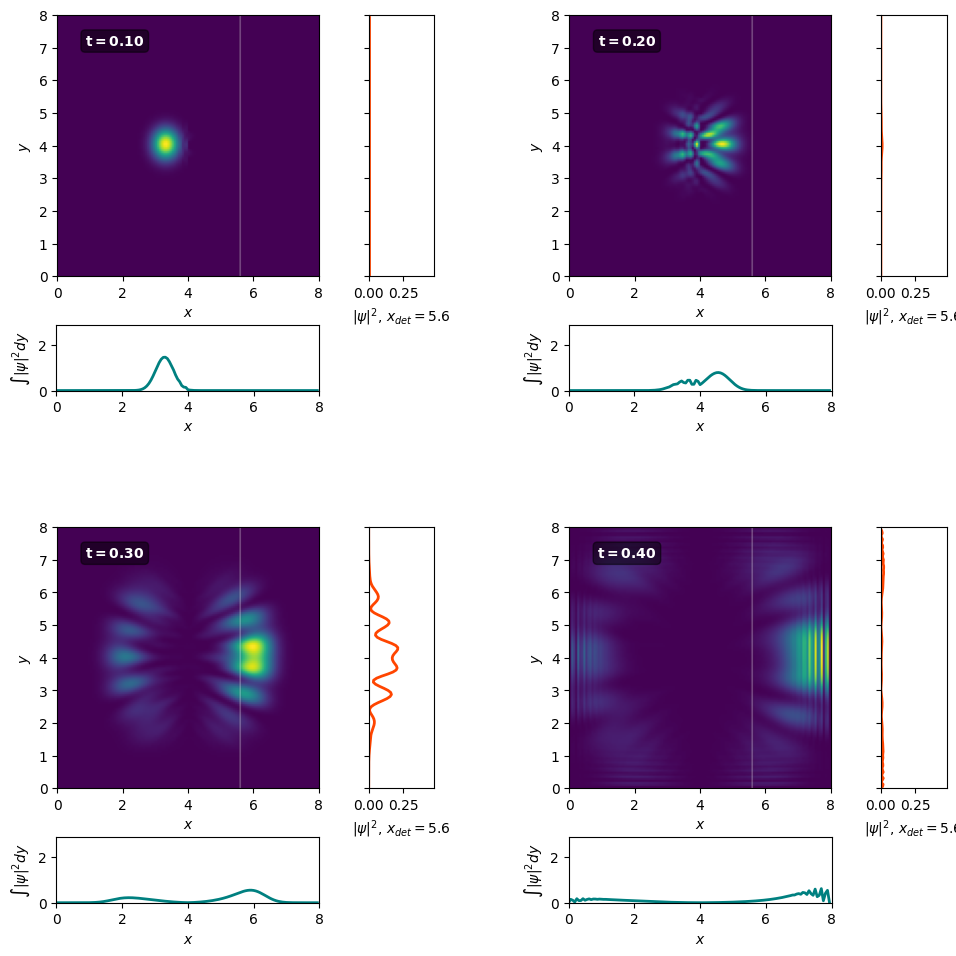
\includegraphics[width=0.7\linewidth]{images/19/no_pot/diff_grate.png}
    \caption{Reticolo di diffrazione, non è visibile il potenziale.}
    \label{fig:placeholder}
\end{figure}


\bigskip\noindent
Le \textit{feature} più importanti che vengono mostrate nelle figure (statiche o animazioni) sono:
\begin{itemize}
    \item Sulla destra un plot che imita il comportamento di un sensore: è anche indicato sul grafico con una semplice linea per corrispondenza con l'evoluzione spaziale, e l'idea è quella di rappresentare $|\psi(x_{det}, y , t_i)|^2= f(y),\ mx_{det}=0.7 mL$, cioè la sezione alla posizione fissata $x_{det}$.
    \item In basso è riportato $\int_0^{L}|\psi(x, y, t_i)|^2dy$. Questo per osservare come la distribuzione della probabilità, che si mantiene cumulativa ad 1 su tutto il dominio, si evolve in funzione del tempo. Grazie a questa visualizzazione abbiamo una rappresentazione più tridimensionale del fenomeno, costruiamo il vero e proprio profilo lungo l'asse x della fdo.
\end{itemize}


\bigskip\noindent
Infine voglio far notare come sia possibile vedere delle figure di intereferenza ai bordi della scatola che rappresenta il nostro dominio, in particolare negli istanti finali dell'animazione: questo è dovuto all'interazione costruttiva e distruttiva di due onde che si propagano con fasi diverse, in particolare quella che procede contro la parete e quella che ci si riflette con fase opposta.\\
Nella maniera in cui abbiamo impostato l'algoritmo, usando \textit{np.roll()}, le condizioni periodiche sono naturalmente incluse nell'evoluzione del sistema, la scelta che faccio è quella di settare le condizioni di Dirichlet, cioè fissare nulla la fdo al contorno: se viene fatto ciò risulta una riflessione totale dell'onda incidente, che può poi interferire come abbiamo appena spiegato. Questo fenomeno è in realtà indesiderabile, poiché rappresenta il limite che ci è consentito dallo studio numerico e discretizzato su un reticolo.\\
Una possibile soluzione potrebbe risiedere nell'allargare il dominio di studio, oppure nel indagare un fenomeno per un tempo sufficientemente breve da non considerare l'interazione della funzione d'onda con le pareti e la conseguente interferenza.

\newpage
% \thispagestyle{empty} 
\null 
\clearpage



\end{document}



% FINE DEL REPORT! (finalmente)